%%%%%%%%%%%%%%%%%%%%%%%%%%%%%%%%%%%%%%%%%
%
% Important note:
% Chapter heading images should have a 2:1 width:height ratio,
% e.g. 920px width and 460px height.
%
% The images can be found anywhere, usually on sky surveys websites or the
% Astronomy Picture of the day archive http://apod.nasa.gov/apod/archivepix.html
%
%%%%%%%%%%%%%%%%%%%%%%%%%%%%%%%%%%%%%%%%%
 
%----------------------------------------------------------------------------------------
%	PACKAGES AND OTHER DOCUMENT CONFIGURATIONS
%----------------------------------------------------------------------------------------

\documentclass[11pt,fleqn]{book} % Default font size and left-justified equations

\usepackage[top=3cm,bottom=3cm,left=3.2cm,right=3.2cm,headsep=10pt,letterpaper]{geometry} % Page margins

\usepackage{xcolor} % Required for specifying colors by name
\definecolor{ocre}{RGB}{52,177,201} % Define the orange color used for highlighting throughout the book

% Font Settings
\usepackage{avant} % Use the Avantgarde font for headings
%\usepackage{times} % Use the Times font for headings
\usepackage{mathptmx} % Use the Adobe Times Roman as the default text font together with math symbols from the Sym­bol, Chancery and Com­puter Modern fonts

\usepackage{microtype} % Slightly tweak font spacing for aesthetics
\usepackage[utf8]{inputenc} % Required for including letters with accents
\usepackage[T1]{fontenc} % Use 8-bit encoding that has 256 glyphs

%% Graphics packages
\usepackage{graphicx}
\usepackage{subfig}
\usepackage{subfloat}

\usepackage{physics} % for physics related notation
\usepackage{amsthm}
\usepackage{amssymb}
%\usepackage{unicode-math}
%\usepackage{txfonts}
\usepackage{mathbbol}
%\usepackage{bbold}
\usepackage{bbm}
\usepackage{calrsfs}
\usepackage{calligra} % Math Caligraphy

\usepackage{exsheets}
\usepackage{answers}
\usepackage{probsoln}
\usepackage{enumitem}

\usepackage{kbordermatrix}% http://www.hss.caltech.edu/~kcb/TeX/kbordermatrix.sty
\usepackage{blkarray} % for block matrix with labels
\usepackage{tensor}  %% included here on 15th April 2019
% Bibliography
%\usepackage[style=alphabetic,sorting=nyt,sortcites=true,autopunct=true,babel=hyphen,hyperref=true,abbreviate=false,backref=true,backend=biber]{biblatex}
%\addbibresource{bibliography.bib} % BibTeX bibliography file
%\defbibheading{bibempty}{}

%%%%%%%%%%%%%%%%%%%%%%%%%%%%%%%%%%%%%%%%%
% This is based on the Legrand Orange Book
% Structural Definitions File
%
% The original template (the Legrand Orange Book Template) can be found here --> http://www.latextemplates.com/template/the-legrand-orange-book
%
% Original author of the Legrand Orange Book Template::
% Mathias Legrand (legrand.mathias@gmail.com) with modifications by:
% Vel (vel@latextemplates.com)
%
% Original License:
% CC BY-NC-SA 3.0 (http://creativecommons.org/licenses/by-nc-sa/3.0/)
%
%%%%%%%%%%%%%%%%%%%%%%%%%%%%%%%%%%%%%%%%%
%----------------------------------------------------------------------------------------
%	VARIOUS REQUIRED PACKAGES
%----------------------------------------------------------------------------------------

\usepackage{titlesec} % Allows customization of titles

\usepackage{graphicx} % Required for including pictures
\graphicspath{{Pictures/}} % Specifies the directory where pictures are stored

\usepackage{lipsum} % Inserts dummy text

\usepackage{tikz} % Required for drawing custom shapes

\usepackage[english]{babel} % English language/hyphenation

\usepackage{enumitem} % Customize lists
\setlist{nolistsep} % Reduce spacing between bullet points and numbered lists

\usepackage{booktabs} % Required for nicer horizontal rules in tables

\usepackage{eso-pic} % Required for specifying an image background in the title page

%----------------------------------------------------------------------------------------
%	MAIN TABLE OF CONTENTS
%----------------------------------------------------------------------------------------

\usepackage{titletoc} % Required for manipulating the table of contents

\contentsmargin{0cm} % Removes the default margin
% Chapter text styling
\titlecontents{chapter}[1.25cm] % Indentation
{\addvspace{15pt}\large\sffamily\bfseries} % Spacing and font options for chapters
{\color{ocre!60}\contentslabel[\Large\thecontentslabel]{1.25cm}\color{ocre}} % Chapter number
{}  
{\color{ocre!60}\normalsize\sffamily\bfseries\;\titlerule*[.5pc]{.}\;\thecontentspage} % Page number
% Section text styling
\titlecontents{section}[1.25cm] % Indentation
{\addvspace{5pt}\sffamily\bfseries} % Spacing and font options for sections
{\contentslabel[\thecontentslabel]{1.25cm}} % Section number
{}
{\sffamily\hfill\color{black}\thecontentspage} % Page number
[]
% Subsection text styling
\titlecontents{subsection}[1.25cm] % Indentation
{\addvspace{1pt}\sffamily\small} % Spacing and font options for subsections
{\contentslabel[\thecontentslabel]{1.25cm}} % Subsection number
{}
{\sffamily\;\titlerule*[.5pc]{.}\;\thecontentspage} % Page number
[] 

%----------------------------------------------------------------------------------------
%	MINI TABLE OF CONTENTS IN CHAPTER HEADS
%----------------------------------------------------------------------------------------

% Section text styling
\titlecontents{lsection}[0em] % Indendating
{\footnotesize\sffamily} % Font settings
{}
{}
{}

% Subsection text styling
\titlecontents{lsubsection}[.5em] % Indentation
{\normalfont\footnotesize\sffamily} % Font settings
{}
{}
{}
 
%----------------------------------------------------------------------------------------
%	PAGE HEADERS
%----------------------------------------------------------------------------------------

\usepackage{fancyhdr} % Required for header and footer configuration

\pagestyle{fancy}
\renewcommand{\chaptermark}[1]{\markboth{\sffamily\normalsize\bfseries\chaptername\ \thechapter.\ #1}{}} % Chapter text font settings
\renewcommand{\sectionmark}[1]{\markright{\sffamily\normalsize\thesection\hspace{5pt}#1}{}} % Section text font settings
\fancyhf{} \fancyhead[LE,RO]{\sffamily\normalsize\thepage} % Font setting for the page number in the header
\fancyhead[LO]{\rightmark} % Print the nearest section name on the left side of odd pages
\fancyhead[RE]{\leftmark} % Print the current chapter name on the right side of even pages
\renewcommand{\headrulewidth}{0.5pt} % Width of the rule under the header
\addtolength{\headheight}{2.5pt} % Increase the spacing around the header slightly
\renewcommand{\footrulewidth}{0pt} % Removes the rule in the footer
\fancypagestyle{plain}{\fancyhead{}\renewcommand{\headrulewidth}{0pt}} % Style for when a plain pagestyle is specified

% Removes the header from odd empty pages at the end of chapters
\makeatletter
\renewcommand{\cleardoublepage}{
\clearpage\ifodd\c@page\else
\hbox{}
\vspace*{\fill}
\thispagestyle{empty}
\newpage
\fi}

%----------------------------------------------------------------------------------------
%	THEOREM STYLES
%----------------------------------------------------------------------------------------

\usepackage{amsmath,amsfonts,amssymb,amsthm} % For math equations, theorems, symbols, etc

\newcommand{\intoo}[2]{\mathopen{]}#1\,;#2\mathclose{[}}
\newcommand{\ud}{\mathop{\mathrm{{}d}}\mathopen{}}
\newcommand{\intff}[2]{\mathopen{[}#1\,;#2\mathclose{]}}
\newtheorem{notation}{Notation}[chapter]

%%%%%%%%%%%%%%%%%%%%%%%%%%%%%%%%%%%%%%%%%%%%%%%%%%%%%%%%%%%%%%%%%%%%%%%%%%%
%%%%%%%%%%%%%%%%%%%% dedicated to boxed/framed environements %%%%%%%%%%%%%%
%%%%%%%%%%%%%%%%%%%%%%%%%%%%%%%%%%%%%%%%%%%%%%%%%%%%%%%%%%%%%%%%%%%%%%%%%%%
\newtheoremstyle{ocrenumbox}% % Theorem style name
{0pt}% Space above
{0pt}% Space below
{\normalfont}% % Body font
{}% Indent amount
{\small\bf\sffamily\color{ocre}}% % Theorem head font
{\;}% Punctuation after theorem head
{0.25em}% Space after theorem head
{\small\sffamily\color{ocre}\thmname{#1}\nobreakspace\thmnumber{\@ifnotempty{#1}{}\@upn{#2}}% Theorem text (e.g. Theorem 2.1)
\thmnote{\nobreakspace\the\thm@notefont\sffamily\bfseries\color{black}---\nobreakspace#3.}} % Optional theorem note
\renewcommand{\qedsymbol}{$\blacksquare$}% Optional qed square

\newtheoremstyle{blacknumex}% Theorem style name
{5pt}% Space above
{5pt}% Space below
{\normalfont}% Body font
{} % Indent amount
{\small\bf\sffamily}% Theorem head font
{\;}% Punctuation after theorem head
{0.25em}% Space after theorem head
{\small\sffamily{\tiny\ensuremath{\blacksquare}}\nobreakspace\thmname{#1}\nobreakspace\thmnumber{\@ifnotempty{#1}{}\@upn{#2}}% Theorem text (e.g. Theorem 2.1)
\thmnote{\nobreakspace\the\thm@notefont\sffamily\bfseries---\nobreakspace#3.}}% Optional theorem note

\newtheoremstyle{blacknumbox} % Theorem style name
{0pt}% Space above
{0pt}% Space below
{\normalfont}% Body font
{}% Indent amount
{\small\bf\sffamily}% Theorem head font
{\;}% Punctuation after theorem head
{0.25em}% Space after theorem head
{\small\sffamily\thmname{#1}\nobreakspace\thmnumber{\@ifnotempty{#1}{}\@upn{#2}}% Theorem text (e.g. Theorem 2.1)
\thmnote{\nobreakspace\the\thm@notefont\sffamily\bfseries---\nobreakspace#3.}}% Optional theorem note

%%%%%%%%%%%%%%%%%%%%%%%%%%%%%%%%%%%%%%%%%%%%%%%%%%%%%%%%%%%%%%%%%%%%%%%%%%%
%%%%%%%%%%%%% dedicated to non-boxed/non-framed environements %%%%%%%%%%%%%
%%%%%%%%%%%%%%%%%%%%%%%%%%%%%%%%%%%%%%%%%%%%%%%%%%%%%%%%%%%%%%%%%%%%%%%%%%%
\newtheoremstyle{ocrenum}% % Theorem style name
{5pt}% Space above
{5pt}% Space below
{\normalfont}% % Body font
{}% Indent amount
{\small\bf\sffamily\color{ocre}}% % Theorem head font
{\;}% Punctuation after theorem head
{0.25em}% Space after theorem head
{\small\sffamily\color{ocre}\thmname{#1}\nobreakspace\thmnumber{\@ifnotempty{#1}{}\@upn{#2}}% Theorem text (e.g. Theorem 2.1)
\thmnote{\nobreakspace\the\thm@notefont\sffamily\bfseries\color{black}---\nobreakspace#3.}} % Optional theorem note
\renewcommand{\qedsymbol}{$\blacksquare$}% Optional qed square
\makeatother

% Defines the theorem text style for each type of theorem to one of the three styles above
\newcounter{dummy} 
\numberwithin{dummy}{section}
\theoremstyle{ocrenumbox}
\newtheorem{theoremeT}[dummy]{Theorem}
\newtheorem{problem}{Problem}[chapter]
\newtheorem{exerciseT}{Exercise}[chapter]
\theoremstyle{blacknumex}
\newtheorem{exampleT}{Example}[chapter]
\theoremstyle{blacknumbox}
\newtheorem{vocabulary}{Vocabulary}[chapter]
\newtheorem{definitionT}{Definition}[section]
\newtheorem{corollaryT}[dummy]{Corollary}
\theoremstyle{ocrenum}
\newtheorem{proposition}[dummy]{Proposition}

%----------------------------------------------------------------------------------------
%	DEFINITION OF COLORED BOXES
%----------------------------------------------------------------------------------------

\RequirePackage[framemethod=default]{mdframed} % Required for creating the theorem, definition, exercise and corollary boxes

% Theorem box
\newmdenv[skipabove=7pt,
skipbelow=7pt,
backgroundcolor=black!5,
linecolor=ocre,
innerleftmargin=5pt,
innerrightmargin=5pt,
innertopmargin=5pt,
leftmargin=0cm,
rightmargin=0cm,
innerbottommargin=5pt]{tBox}

% Exercise box	  
\newmdenv[skipabove=7pt,
skipbelow=7pt,
rightline=false,
leftline=true,
topline=false,
bottomline=false,
backgroundcolor=ocre!10,
linecolor=ocre,
innerleftmargin=5pt,
innerrightmargin=5pt,
innertopmargin=5pt,
innerbottommargin=5pt,
leftmargin=0cm,
rightmargin=0cm,
linewidth=4pt]{eBox}	

% Definition box
\newmdenv[skipabove=7pt,
skipbelow=7pt,
rightline=false,
leftline=true,
topline=false,
bottomline=false,
linecolor=ocre,
innerleftmargin=5pt,
innerrightmargin=5pt,
innertopmargin=0pt,
leftmargin=0cm,
rightmargin=0cm,
linewidth=4pt,
innerbottommargin=0pt]{dBox}	

% Corollary box
\newmdenv[skipabove=7pt,
skipbelow=7pt,
rightline=false,
leftline=true,
topline=false,
bottomline=false,
linecolor=gray,
backgroundcolor=black!5,
innerleftmargin=5pt,
innerrightmargin=5pt,
innertopmargin=5pt,
leftmargin=0cm,
rightmargin=0cm,
linewidth=4pt,
innerbottommargin=5pt]{cBox}

% Creates an environment for each type of theorem and assigns it a theorem text style from the "Theorem Styles" section above and a colored box from above
\newenvironment{theorem}{\begin{tBox}\begin{theoremeT}}{\end{theoremeT}\end{tBox}}
\newenvironment{exercise}{\begin{eBox}\begin{exerciseT}}{\hfill{\color{ocre}\tiny\ensuremath{\blacksquare}}\end{exerciseT}\end{eBox}}				  
\newenvironment{definition}{\begin{dBox}\begin{definitionT}}{\end{definitionT}\end{dBox}}	
\newenvironment{example}{\begin{exampleT}}{\hfill{\tiny\ensuremath{\blacksquare}}\end{exampleT}}		
\newenvironment{corollary}{\begin{cBox}\begin{corollaryT}}{\end{corollaryT}\end{cBox}}	

%----------------------------------------------------------------------------------------
%	REMARK ENVIRONMENT
%----------------------------------------------------------------------------------------

\newenvironment{remark}{\par\vspace{10pt}\small % Vertical white space above the remark and smaller font size
\begin{list}{}{
\leftmargin=35pt % Indentation on the left
\rightmargin=25pt}\item\ignorespaces % Indentation on the right
\makebox[-2.5pt]{\begin{tikzpicture}[overlay]
\node[draw=ocre!60,line width=1pt,circle,fill=ocre!25,font=\sffamily\bfseries,inner sep=2pt,outer sep=0pt] at (-15pt,0pt){\textcolor{ocre}{R}};\end{tikzpicture}} % Orange R in a circle
\advance\baselineskip -1pt}{\end{list}\vskip5pt} % Tighter line spacing and white space after remark

%----------------------------------------------------------------------------------------
%	SECTION NUMBERING IN THE MARGIN
%----------------------------------------------------------------------------------------

\makeatletter
\renewcommand{\@seccntformat}[1]{\llap{\textcolor{ocre}{\csname the#1\endcsname}\hspace{1em}}}                    
\renewcommand{\section}{\@startsection{section}{1}{\z@}
{-4ex \@plus -1ex \@minus -.4ex}
{1ex \@plus.2ex }
{\normalfont\large\sffamily\bfseries}}
\renewcommand{\subsection}{\@startsection {subsection}{2}{\z@}
{-3ex \@plus -0.1ex \@minus -.4ex}
{0.5ex \@plus.2ex }
{\normalfont\sffamily\bfseries}}
\renewcommand{\subsubsection}{\@startsection {subsubsection}{3}{\z@}
{-2ex \@plus -0.1ex \@minus -.2ex}
{.2ex \@plus.2ex }
{\normalfont\small\sffamily\bfseries}}                        
\renewcommand\paragraph{\@startsection{paragraph}{4}{\z@}
{-2ex \@plus-.2ex \@minus .2ex}
{.1ex}
{\normalfont\small\sffamily\bfseries}}

%----------------------------------------------------------------------------------------
%	HYPERLINKS IN THE DOCUMENTS
%----------------------------------------------------------------------------------------

% For an unclear reason, the package should be loaded now and not later
\usepackage{hyperref}
%\hypersetup{hidelinks,backref=true,pagebackref=true,hyperindex=true,colorlinks=false,breaklinks=true,urlcolor= ocre,bookmarks=true,bookmarksopen=false,pdftitle={Title},pdfauthor={Author}}

%----------------------------------------------------------------------------------------
%	CHAPTER HEADINGS
%----------------------------------------------------------------------------------------

% The set-up below should be (sadly) manually adapted to the overall margin page septup controlled by the geometry package loaded in the main.tex document. It is possible to implement below the dimensions used in the goemetry package (top,bottom,left,right)... TO BE DONE

\newcommand{\thechapterimage}{}
\newcommand{\chapterimage}[1]{\renewcommand{\thechapterimage}{#1}}

% Numbered chapters with mini tableofcontents
\def\thechapter{\arabic{chapter}}
\def\@makechapterhead#1{
\thispagestyle{empty}
{\centering \normalfont\sffamily
\ifnum \c@secnumdepth >\m@ne
\if@mainmatter
\startcontents
\begin{tikzpicture}[remember picture,overlay]
\node at (current page.north west)
{\begin{tikzpicture}[remember picture,overlay]
\node[anchor=north west,inner sep=0pt] at (0,0) {\includegraphics[width=\paperwidth]{\thechapterimage}};
%%%%%%%%%%%%%%%%%%%%%%%%%%%%%%%%%%%%%%%%%%%%%%%%%%%%%%%%%%%%%%%%%%%%%%%%%%%%%%%%%%%%%
% Commenting the 3 lines below removes the small contents box in the chapter heading
%\fill[color=ocre!10!white,opacity=.6] (1cm,0) rectangle (8cm,-7cm);
%\node[anchor=north west] at (1.1cm,.35cm) {\parbox[t][8cm][t]{6.5cm}{\huge\bfseries\flushleft \printcontents{l}{1}{\setcounter{tocdepth}{2}}}};
\draw[anchor=west] (5cm,-9cm) node [rounded corners=20pt,fill=ocre!10!white,text opacity=1,draw=ocre,draw opacity=1,line width=1.5pt,fill opacity=.6,inner sep=12pt]{\huge\sffamily\bfseries\textcolor{black}{\thechapter. #1\strut\makebox[22cm]{}}};
%%%%%%%%%%%%%%%%%%%%%%%%%%%%%%%%%%%%%%%%%%%%%%%%%%%%%%%%%%%%%%%%%%%%%%%%%%%%%%%%%%%%%
\end{tikzpicture}};
\end{tikzpicture}}
\par\vspace*{230\p@}
\fi
\fi}

% Unnumbered chapters without mini tableofcontents (could be added though) 
\def\@makeschapterhead#1{
\thispagestyle{empty}
{\centering \normalfont\sffamily
\ifnum \c@secnumdepth >\m@ne
\if@mainmatter
\begin{tikzpicture}[remember picture,overlay]
\node at (current page.north west)
{\begin{tikzpicture}[remember picture,overlay]
\node[anchor=north west,inner sep=0pt] at (0,0) {\includegraphics[width=\paperwidth]{\thechapterimage}};
\draw[anchor=west] (5cm,-9cm) node [rounded corners=20pt,fill=ocre!10!white,fill opacity=.6,inner sep=12pt,text opacity=1,draw=ocre,draw opacity=1,line width=1.5pt]{\huge\sffamily\bfseries\textcolor{black}{#1\strut\makebox[22cm]{}}};
\end{tikzpicture}};
\end{tikzpicture}}
\par\vspace*{230\p@}
\fi
\fi
}
\makeatother % Insert the commands.tex file which contains the majority of the structure behind the template
% For big zero in block matrix
\newcommand{\bigzero}{\mbox{\normalfont\Large\bfseries 0}}

\renewcommand{\kbldelim}{(}% Left delimiter
\renewcommand{\kbrdelim}{)}% Right delimiter


\newcommand{\iu}{{i\mkern1mu}}





%%% by kabir sir


\newcommand{\be}{\begin{equation}}
\newcommand{\ee}{\end{equation}}
\newcommand{\p}{\paragraph}
\newcommand{\La}{\Lambda}
\newcommand{\ec}{\end{center}}
\newcommand{\ba}{\begin{eqnarray}}
\newcommand{\ea}{\end{eqnarray}}
\DeclareRobustCommand{\rchi}{{\mathpalette\irchi\relax}}
\newcommand{\irchi}[2]{\raisebox{\depth}{$#1\chi$}} % inner command, used by \rchi


\sloppy
%\fussy
\nonfrenchspacing
%\hspace{12pt}
%\topmargin - 0.5 in
%\hoffset - 9 mm
%\text height 24 cm
%\leftmargin- 0.5 in
%\bottommargin - 0.5 in
%\rightmargin - 0.5 i
\renewcommand{\baselinestretch}{1.3} 

\begin{document}
\title{Quantum Mechanics}

%----------------------------------------------------------------------------------------
%	TITLE PAGE
%----------------------------------------------------------------------------------------

\begingroup
\thispagestyle{empty}
\AddToShipoutPicture*{\put(0,0){\includegraphics[scale=1.25]{esahubble}}} % Image background
\centering
\vspace*{5cm}
\par\normalfont\fontsize{35}{35}\sffamily\selectfont
\textbf{Quantum Mechanics}\\
{\LARGE Lecture Notes}\par % Book title
\vspace*{1cm}
{\Huge Dr. Khorshed Kabir}\par % Author name
\endgroup

%----------------------------------------------------------------------------------------
%	COPYRIGHT PAGE
%----------------------------------------------------------------------------------------

\newpage
~\vfill
\thispagestyle{empty}

%\noindent Copyright \copyright\ 2014 Andrea Hidalgo\\ % Copyright notice



%\noindent %\textsc{github.com/LaurethTeX/Clustering}\\ % URL

{\noindent This notes are compiled under supervision of Dr. Khorshed Kabir}\\ % License information

{\noindent \textsc{University of Dhaka}}\\

{\noindent \textit{First release, %August
	 2019}} % Printing/edition date

%----------------------------------------------------------------------------------------
%	CREDITS PAGE
%----------------------------------------------------------------------------------------

\newpage


Thanks to the following individuals \\
%\vfill
{\centering
Muhammad Shahnoor Rahman, Department of Physics, University of Dhaka.\\}



%----------------------------------------------------------------------------------------
%	TABLE OF CONTENTS
%----------------------------------------------------------------------------------------

\chapterimage{Pictures/head1.png} % Table of contents heading image

\pagestyle{empty} % No headers

\tableofcontents % Print the table of contents itself

%\cleardoublepage % Forces the first chapter to start on an odd page so it's on the right

\pagestyle{fancy} % Print headers again
%\pagestyle{headings} % Print headers again

%----------------------------------------------------------------------------------------
%	CHAPTERS
%----------------------------------------------------------------------------------------

%\chapterimage{head2.png} % Chapter heading image

\chapter{sheet-1 :Dirac Delta Function}
\label{chapter1.dirac-delta}

\ifpdf
\graphicspath{{Chapter1/figs/}}
\else
\graphicspath{{Chapter1/figs/}}
\fi

%\chapterimage{head2.png} % Chapter heading image

%\chapter{sheet-1 :Dirac Delta Function}


	Consider the function $D_\epsilon(x)$ given by
	\begin{eqnarray}
	D_\epsilon(x) &= 
		\begin{cases}
			\frac{1}{\epsilon} \ \ &\text{for} \ \  -\frac{\epsilon}{2} \leq x \leq \frac{\epsilon}{2} \\
			0 \ \ &\text{for} \ \  |x| > \frac{\epsilon}{2} 
		\end{cases}
	\end{eqnarray}
	where $\epsilon$ is a positive parameter. The plot of the function is shown in figure (\ref{fig.cpt1.figure1}).
	
	\begin{figure}
		\centering
		\subfloat[]{\includegraphics[width=5cm]{delta.pdf}}
		\caption{Dirac Delta Function}
		\label{fig.cpt1.figure1}
	\end{figure}
	
	The integral of the function with respect to $x$ is $1$, i.e.,
	\begin{equation}
		\int_{-\infty}^{\infty} D_\epsilon(x) dx = 1
	\end{equation}
	Now imagine making $\epsilon$ smaller. As we decrease $\epsilon$, the function gets narrower and taller, but the integral of the function(i.e., the area under graph remains constant at the value $1$).
	In the limit $\epsilon \rightarrow 0$, the function $D_\epsilon(x)$ collapses to a single  point $x=0$ and gets infinitely tall. So $\lim\limits_{\epsilon \rightarrow \epsilon} D_\epsilon(x)$ is not a function at all and the procedure of taking the limit is not justified.
	\\
	
	However, we can make the limiting procedure meaningful if multiply $D_\epsilon(x)$ by some well defined function $f(x)$, integrate over $x$ and then take the limit $\epsilon \rightarrow 0 $. consider the integral
	\begin{equation}
		\int_{-\infty}^{\infty} D_\epsilon(x) f(x) dx
	\end{equation}
	where $f(x)$ is a well-defined function. If $\epsilon$ is significantly small, the variation of $f(x)$ over the effective integration interval $[-\epsilon / 2, \epsilon / 2]$ is negligible and $f(x)$ remains practically equal to $f(0)$, therefore,
	\begin{equation}
		\int_{-\infty}^{\infty} D_\epsilon (x) f(x) dx \simeq f(0) \int_{-\infty}^{\infty} D_\epsilon (x) dx = f(0)
	\end{equation}
	The smaller the value of $\epsilon$, the better the approximation. In the limit $\epsilon \rightarrow 0$, the above equation is exact
	\begin{equation}
		\lim\limits_{\epsilon \rightarrow 0}\int_{-\infty}^{\infty} D_\epsilon (x) f(x) dx  = f(0)
	\end{equation}
	Now, we define the delta function by the relation
	\begin{equation}
		\int_{-\infty}^{\infty} \delta(x) f(x) dx \  _=^{def}  \lim\limits_{\epsilon \rightarrow 0}\int_{-\infty}^{\infty} D_\epsilon (x) f(x) dx  = f(0)
	\end{equation}
	This equation is valid for any function $f(x)$ defined at the origin. More generally, $\delta(x - x_0)$ is defined as,
	\begin{equation}
		\int_{-\infty}^{\infty} \delta(x - x_0) f(x) dx \ = f(x_0)
	\end{equation}
	Actually, the integral notation $\int_{-\infty}^{\infty} \delta(x) f(x) dx$ is not justified because $\delta(x)$ is not really a function. Physically, there is no problem since it becomes impossible to distinguish between $D_\epsilon(x)$ and $\delta(x)$ as soon as $\epsilon$ becomes negligible compared to all distances involved in a physical problem. Whenever a mathematical difficulty might arise, all we need to do is to assume that $\delta(x)$ is actually $D_\epsilon(x)$ with $\epsilon$ extremely small but not strictly zero.
	\\
	Formally, we can express $\delta(x)$ as a limit of a square of proper functions : 
	\begin{equation}
		\lim\limits_{\epsilon \rightarrow 0} D_\epsilon(x) \equiv \delta(x)
	\end{equation}
	Here $D_\epsilon(x)$, which is a proper function of $x$ is called the representation of the delta function. One representation is the "square function" given at the beginning. The representation is not unique. There are other functions which approach the delta function when appropriate limits are taken.
	
	\section{Other representation of delta function}
		\begin{enumerate}
			\item 
			Consider the function
			\begin{equation}
				D_\epsilon(x) = \frac{1}{\epsilon \sqrt{\pi}} e^{-x^2/\epsilon^2}  \ \ \ (\epsilon > 0)
				\label{eqn.other-reps-exp}
			\end{equation}
			For each value of the parameter $\epsilon$, this function satisfies
			\begin{equation}
			\int_{-\infty}^{\infty} D_\epsilon(x) dx = 1
			\end{equation}
		
		\begin{figure}
			\centering
			\subfloat[]{\includegraphics[width=5cm]{chapter1-delta-reps-exp.pdf}}
			\subfloat[]{\includegraphics[width=5cm]{chapter1-delta-reps-sine.pdf}}
			\caption{Plot of function $D_\epsilon(x)$ for (a) equation (\ref{eqn.other-reps-exp}) (b) and equation (\ref{eqn.other-reps-sin})}
			\label{fig.cpt1.figure2}
		\end{figure}
		
		
		When plotted against $x$, the function has a peak at the origin. The peak has a height of $\frac{1}{\epsilon \sqrt{\pi}}$ and a width of order $\epsilon$ (exactly how the width is defined doesn't matter). So if $\epsilon$ is allowed to become very small, the peak becomes very tall and very narrow. Outside the peak the function becomes extremely small. Thus we have
		\begin{equation}
		\delta(x) = \lim\limits_{\epsilon \rightarrow 0}\frac{1}{\epsilon \sqrt{\pi}} e^{-x^2/\epsilon^2}
		\end{equation}
		
		%% proof
		
		\item
		Consider another function
		\begin{equation}
			D_\epsilon(x) = \frac{1}{\pi} \frac{\sin(x/\epsilon)}{x} \ \ \ \ (\epsilon > 0)
			\label{eqn.other-reps-sin}
		\end{equation} 
		

		
		For any value of the parameter $\epsilon$ we have 
		\begin{equation}
			\int_{-\infty}^{\infty} D_\epsilon(x) dx = 1
		\end{equation}
		A plot of the function $D_\epsilon(x)$ shows that it has the value $\frac{1}{\epsilon \pi}$ at $x=0$ and it oscillates with decreasing amplitude as $|x|$ increases. The width of the central maxima is of the order of $\epsilon$ and the period of oscillation with respect to $x$ is $2 \pi \epsilon$.\\
		Thus the limit of this function as $\epsilon \rightarrow 0 $ has all the properties of the delta function : it becomes infinitely large at $x=0$, it has unit integral, and infinitely rapid oscillations as $|x|$ increases means that the entire contribution to an integral containing this function comes from an infinitesimal neighborhood of $x=0$.\\
		We can therefore write,
		\begin{equation}
			\delta(x) = \lim\limits_{\epsilon \rightarrow 0} \frac{1}{\pi} \frac{\sin(x/\epsilon)}{x}
		\end{equation}

		\item
		We can also show that
		\begin{eqnarray}
			\delta(x) &= \lim\limits_{\epsilon \rightarrow 0} \frac{1}{2\epsilon} e^{-|x| / \epsilon} \\
			\delta(x) &= \lim\limits_{\epsilon \rightarrow 0} \frac{1}{\pi} \frac{\epsilon}{x^2 + \epsilon^2} \\
			\delta(x) &= \lim\limits_{\epsilon \rightarrow 0} \frac{\epsilon}{\pi} \frac{\sin^2(x/\epsilon)}{x^2}
		\end{eqnarray}
		
		\end{enumerate}	
	\section{Properties of the delta function}
		It is important to note that, because of its singular $@@@@@@$ , the $\delta$ function cannot be the end result of a calculation, and has meaning only so long as a subsequent integral over its argument is carried out. With this understanding we can write down some relations between delta functions.
		\begin{enumerate}[label=\textbf{Property \ \arabic*},start=1]
			\item 
			The delta function is a even function
			\begin{equation}
				\delta(-x) = \delta(x)
			\end{equation}
			
			\item
			\begin{equation}
				x \delta(x) = 0
			\end{equation}
			
			\item
			\begin{equation}
			\delta(a x) = \frac{1}{|a|} \delta(x)
			\end{equation}
			proof: Consider the integral
			\begin{equation}
				I = \int_{-\infty}^{\infty} \delta(a x) f(x) dx
			\end{equation}
			Since the delta function is even in its argument, it doesn't matter if we replace $a$ by $|a|$ in the argument. Thus
			\begin{equation}
				I = \int_{-\infty}^{\infty} \delta(|a| x) f(x) dx
			\end{equation}
			Making the change in variable $ y = |a| x$ we have,
			\begin{eqnarray}
				I &= \frac{1}{|a|}\int_{-\infty}^{\infty} \delta(y) f(y/|a|) dx \nonumber \\
				&= \frac{1}{|a|} f(0) \nonumber
			\end{eqnarray}			
			or
			\begin{equation}
				\int_{-\infty}^{\infty} \delta(a x) f(x) dx = \frac{1}{|a|} \int_{-\infty}^{\infty} \delta(x) f(x) dx
			\end{equation}
			or
			\begin{equation}
				\delta(a x) = \frac{1}{|a|} \delta(x)
			\end{equation}
			
			
			\item
			More generally
			\begin{equation}
				\delta(\phi(x)) = \sum_{i} \frac{\delta(x - x_i)}{\left|\frac{\partial\phi}{\partial x}\right|_{x_i}}
			\end{equation}
			where the sum sums over the $x_i$'s which are simple roots of $\phi(x)$.
			
			proof : let $x_1 , x_2, \ldots , x_N$ be the simple roots of $\phi(x)$,
			
			%figure
			
			In the neighborhood of any one of the simple roots $x_i$, we can write
			@@@@@@@
			\begin{equation}
				\phi(x) = (x - x_i) \psi(x)
			\end{equation}
			or ???????
			\begin{equation}
				\phi(x) = (x - x_i) \psi(x_i)
			\end{equation}
			
			where $\psi(x_i) \neq 0$. We have
			\begin{equation}
				\psi(x_i) = \left|\frac{\partial \phi(x)}{\partial x} \right|_{x=x_i}
			\end{equation}
			Now, consider the integral
			\begin{eqnarray}
				I &= \int_{-\infty}^{\infty} \delta(\phi(x)) f(x) dx  \nonumber \\
				&= \sum_{i=1}^{N} \int_{x_i - \epsilon}^{x_i + \epsilon} \delta[(x-x_i) \psi(x_i)] f(x) dx \nonumber \\
				&= \sum_{i=1}^{N} \frac{1}{|\psi(x_i)|}\int_{x_i - \epsilon}^{x_i + \epsilon} \delta(x-x_i) f(x) dx \nonumber \\
				&= \sum_{i=1}^{N} \frac{1}{ \left|\frac{\partial \phi(x)}{\partial x} \right|_{x=x_i}}\int_{-\infty}^{\infty} \delta(x-x_i) f(x) dx \nonumber \\
				&= \sum_{i=1}^{N} \frac{1}{ \left|\frac{\partial \phi}{\partial x} \right|_{x=x_i}} f(x_i) \nonumber
			\end{eqnarray}
			The above result is obtained if we write
			\begin{equation}
				\delta(\phi(x)) = \sum_{i=1}^{N} \frac{\delta(x - x_i)}{\left|\frac{\partial \phi}{\partial x}\right|_{x=x_i}}
			\end{equation}
			
			
			\item
			A frequently used example of the above result is
			\begin{equation}
				\delta(x^2 - a^2) = \frac{1}{2 a} \delta(x - a) + \frac{1}{2 a} \delta(x + a) \ \ \ \ (a > 0)
			\end{equation}
			
			Here
			\begin{equation}
				\phi(x) = x^2 - a^2 = (x-a)(x+a)
			\end{equation}
				The two simple roots of $\phi(x)$ are at $x=a $ and $x=-a$. Now
				\begin{eqnarray}
					\left|\frac{\partial \phi}{\partial x}\right|_{x=a} = \left|2 x\right|_{x=a} = 2a  \\
					\left|\frac{\partial \phi}{\partial x}\right|_{x=a} = \left|-2 x\right|_{x=-a} = 2a 
				\end{eqnarray}
				$\therefore$ The above result follows.
				
				\item
				\begin{equation}
					f(x) \delta(x-a) = f(a) \delta(x-a)
				\end{equation}

				\item
				\begin{equation}
					\int \delta(x-y) \delta(y-a) dy = \delta(x-a)
				\end{equation}
				
			
		\end{enumerate}
		
		\subsection{Notes}
		\begin{enumerate}[label=\textbf{Note : \ \arabic*},start=1]
			\item 
			We have the identity
			\begin{equation}
				x\delta(x) = 0
			\end{equation}
			The converse is also true and it can be shown that the equation
			\begin{equation}
				x u(x) = 0
			\end{equation}
			has the general solution
			\begin{equation}
				u(x) = c \delta(x)
			\end{equation}
			
			
			\item
			We will now prove an identity which is particularly useful in Quantum Mechanics.
			\begin{equation}
				\lim\limits_{\epsilon \rightarrow 0^+} \int_{-\infty}^{\infty} \frac{1}{x \pm \imath \epsilon} f(x) dx = \rho \int_{-\infty}^{\infty} \frac{dx}{x}f(x) \mp \imath\pi f(0)
			\end{equation}
			or in short
			\begin{equation}
				\lim\limits_{\epsilon \rightarrow 0^+} \frac{1}{x \pm \imath \epsilon} = \rho(\frac{1}{x}) \mp \imath \pi \delta(x)
			\end{equation}
			Where it is understood that the second of these two equations have meaning only within an integral.\\
			The symbol $\rho$ means principle part of an integral where the integral has a single pole. The principle part is defined as
			\begin{equation}
				\rho \int_{-A}^{B} \frac{dx}{x} f(x) dx = \lim\limits_{\eta \rightarrow 0^+} \left[\int_{-A}^{-\eta} + \int_{\eta}^{B}\right] \frac{dx}{x} f(x)
			\end{equation}
			\textbf{proof :}
			\begin{equation}
				\frac{1}{x \pm \imath \epsilon} = \frac{x \mp \imath\epsilon}{x^2 + \epsilon^2} = \frac{x}{x^2 + \epsilon^2} \mp \frac{\imath \epsilon}{x^2 + \epsilon^2}
			\end{equation}
			Now we have
			\begin{eqnarray}\label{eqn:1}
				\lim\limits_{\epsilon \rightarrow 0^+} \frac{1}{\pi} \frac{\epsilon}{x^2 + \epsilon^2} &= \delta(x) \nonumber \\
				\lim\limits_{\epsilon \rightarrow 0^+} (\mp) \imath \frac{\epsilon}{x^2 + \epsilon^2} &= \mp \imath \pi \delta(x)
			\end{eqnarray}
			Now consider the first term on the right hand side of equation  \ref{eqn:1}. We multiply this term by a function $f(x)$ which is regular at the origin and then integrate over $x$. We get
			\begin{equation}\label{eqn:2}
				\lim\limits_{\epsilon \rightarrow 0^+} \int_{-\infty}^{\infty} \frac{x f(x)}{x^2 + \epsilon^2} dx
				=\lim\limits_{\epsilon \rightarrow 0^+}\left[
				\lim\limits_{\eta \rightarrow 0^+}\left[ \int_{-\infty}^{-\eta} \frac{x f(x)}{x^2 + \epsilon^2}
				+\int_{-\eta}^{\eta} \frac{x f(x)}{x^2 + \epsilon^2}
				+\int_{\eta}^{\infty} \frac{x f(x)}{x^2 + \epsilon^2} dx\right]\right]
			\end{equation}
			Note that we take the limit over $\eta$ first and then we take the limit over $\epsilon$. Consider now the second integral above
			\begin{equation} 
				\lim\limits_{\eta \rightarrow 0^+} \int_{-\eta}^{+\eta} \frac{x f(x)}{x^2 + \epsilon^2} = f(0) \lim\limits_{\eta \rightarrow 0^+} \frac{1}{2}  \left[\ln({x^2 + \epsilon^2}
				)\right]_{x=-\eta}^{x=\eta} = 0
			\end{equation}
			If we now reverse the order of the evaluation of limits in equation \ref{eqn:2}, the $\epsilon \rightarrow 0$ limit causes no difficulties in the other two integrals.
			Thus we have
			\begin{eqnarray}
				&\lim\limits_{\epsilon \rightarrow 0^+} \int_{-\infty}^{\infty} \frac{x dx}{x^2 + \epsilon^2} f(x)\nonumber \\
				 = &\lim\limits_{\eta \rightarrow 0^+} \lim\limits_{\epsilon \rightarrow 0^+} \left[\int_{-\infty}^{-\eta} + \int_{\eta}^{\infty}\right] \frac{x dx}{x^2 + \epsilon^2} f(x) \nonumber \\
				 = &\lim\limits_{\eta \rightarrow 0^+} \left[\int_{-\infty}^{-\eta} + \int_{\eta}^{\infty}\right] \frac{dx}{x} f(x) \nonumber\\
				 = & \rho \int_{-\infty}^{\infty} \frac{1}{x} f(x) dx \nonumber
			\end{eqnarray}
			This establishes the identity.
		\end{enumerate}
		
	\section{Derivatives of the delta function}
		One may define the derivative $\delta^\prime(x)$ of the delta function. When $\epsilon$ is small, the derivative of $D_\epsilon(x)$ has two peaks close to the origin, one peak is positive and the other is negative as drawn in the figure below
		
		\begin{figure}
			\centering
			\subfloat[]{\includegraphics[height=8cm,width=5cm]{chapter1-delta-reps-exp-derivative.pdf}}
			\caption{(a) Derivative of Delta Function}
			\label{}
		\end{figure}
		% figure
		
		
		As $\epsilon \rightarrow 0$, each of these peaks becomes very narrow and very tall, and two peaks each approach very close to the origin. \\
		Now the integration by parts gives
		\begin{equation}
			\int_{-\infty}^{\infty} dx D_\epsilon^\prime(x) f(x) = \left[D_\epsilon(x) f(x)\right]_{-\infty}^{\infty} - \int_{-\infty}^{\infty} dx D_\epsilon(x) f^\prime(x)
		\end{equation}
		Because $D_\epsilon(x)$ tens to zero as $x \rightarrow \pm \infty$, the first term on the right hand side vanishes unless $f(x)$ $@@@@@@@$ violently at infinity. So by letting $\epsilon \rightarrow 0$, we arrive at the definition of $\delta^\prime(x)$
		\begin{equation}\label{eqn:3}
			\int_{-\infty}^{\infty} \delta^\prime(x) f(x) dx = - \int_{-\infty}^{\infty} \delta(x) f^\prime(x) dx = - f^\prime(0)
		\end{equation}
		From this we immediately get
		\begin{equation}
			x \delta^\prime(x) = -\delta(x)
		\end{equation}
		Conversely, it can be shown that the general solution of the equation
		\begin{equation}
			x u(x) = \delta(x)
		\end{equation}
		can be written as
		\begin{equation}
			u(x) = -\delta^\prime(x) + c \delta(x)
		\end{equation}
		Where the second term arises from the homogeneous equation $x \delta(x) = 0$.
		From equation  \ref{eqn:3}  it also follows that 
		\begin{equation}
			\delta^\prime(-x) = - \delta^\prime(x)
		\end{equation}
		The $n^{th}$ order derivative of $\delta(x)$ can be defined in the same way. We find
		\begin{equation}
			\int_{-\infty}^{\infty} \delta^{(n)}(x) f(x) dx = (-1)^{n} f(0)
		\end{equation}
		We can prove the following properties:
		\begin{eqnarray}
			\delta^{(m)}(x) &= (-1)^m \delta^{(m)} (-x) \\
			x^{m+1} \delta^{(m)}(x) &= 0 \\
			x\delta^{(m)}(x) &= -m \delta^{(m-1)} (x)
		\end{eqnarray}
		
		
	\section{Integration of the delta function}
		Consider the indefinite integral
		\begin{equation}\label{eqn:4}
			\Theta_\epsilon(x) = \int_{-\infty}^{x}  D_\epsilon(y) dy
		\end{equation}
		A graph of $\Theta_\epsilon(x)$ vs $x$ is shown below
		
		%figure
		
		As $\epsilon \rightarrow 0$, the step in the function $\Theta_\epsilon(x)$ gets progressively steeper, until, finally, the function changes abruptly from $0$ to $1$ at $x=0$.
		Thus taking the limit $\epsilon \rightarrow 0$ in equation \ref{eqn:4} we have
		\begin{equation}\label{eqn:5}
			\Theta(x) = \int_{-\infty}^{x} \delta(x) dx
		\end{equation}
		Where
		\begin{equation}
			\Theta(x) = 
			\begin{cases}
				1 \ \ \text{for} \ \ x > 0 \\
				0 \ \ \text{for} \ \ x < 0
			\end{cases}
		\end{equation}
		If we differentiate equation \ref{eqn:5} with respect to $x$,\\
		we get
		\begin{equation}
			\frac{d \Theta(x)}{dx} = \delta(x)
		\end{equation}
		
	\section{Three - dimensional delta function}
		\begin{equation}
			\delta(\vec{r}) _=^{def} \delta(x) \delta(y) \delta(z)
		\end{equation}
		In other words, $\delta(\vec{r})$ is zero if any of the coordinates $x, y, z$ is not equal to zero and $\delta(\vec{r})$ tends to infinity at the origin, i.e., when $x=0, y=0, z=0$, such that 
		\begin{equation}
			\int_{volume} \delta(\vec{r}) d^3 r = 1
		\end{equation}
		if the volume of the integration contains the origin. We also have
		\begin{equation}
			\int \delta(\vec{r}) f(\vec{r}) d^3 r = f(0)
		\end{equation}
		where again the volume of the integration includes the origin.
		\textbf{Note:}
		\begin{eqnarray}
			\delta(\vec{r} - \vec{r^\prime}) &= \delta(x - x^\prime) \delta(y - y^\prime) \delta(z-z^\prime) \\
			\int_{v}\delta(\vec{r} - \vec{r^\prime}) d^3r &= 1
		\end{eqnarray}
		where the volume of integration includes the point $\vec{r}^\prime$. Otherwise the integral is zero.
		\begin{equation}
			\int_{v}\delta(\vec{r} - \vec{r^\prime}) f(\vec{r}) d^3r = f(\vec{r^\prime})
		\end{equation}
		if V includes the point $\vec{r^\prime}$.
		
		\textbf{A useful formula}
		Consider the integral
		\begin{eqnarray}
			\int_{-\infty}^{\infty} e^{\imath k x} dx 
			&= \lim\limits_{L \rightarrow \infty} \int_{-L}^{L} e^{\imath k x} dx \nonumber \\
			&= \lim\limits_{L \rightarrow \infty} \frac{1}{\imath k} \left(e^{\imath k L} - e^{-\imath k L}\right) \nonumber \\
			&= \lim\limits_{L \rightarrow \infty} \frac{2}{k} \left(\frac{e^{\imath k L} - e^{-\imath k L}}{2\imath}\right) \nonumber \\
			&= \lim\limits_{L \rightarrow \infty} \frac{2}{k} \sin(k L) \nonumber \\
			&= 2\pi \lim\limits_{L \rightarrow \infty} \frac{\sin(k L
				)}{\pi k} \nonumber \\
			&= 2\pi \delta(k)
		\end{eqnarray}
		using 
		\begin{equation}
			\lim\limits_{\epsilon \rightarrow 0} \frac{\sin(x /\epsilon
				)}{\pi x} = \delta(x)
		\end{equation}
		Thus
		\begin{equation}\label{eqn:6}
			\int_{-\infty}^{\infty} e^{\imath k x} dx = 2\pi \delta(k)
		\end{equation}
		In equation \ref{eqn:6} if we integrate with respect to $k$, we would have $delta(x)$ on the right hand side,
	
	%%%%%%%%%%%%%%%%%%%%%%%%%%%% equation number
	
		\begin{equation}\label{eqn:100}
		\int_{-\infty}^{\infty} e^{\imath k x} dk = 2\pi \delta(x)
		\end{equation}
		Also note that in equation \ref{eqn:6} we are integrating over its full range of values. Making a change of variable $x \rightarrow -x$ does not change the value of the integral. Hence we also have
		
		\begin{equation}\label{eqn:101}
		\int_{-\infty}^{\infty} e^{-\imath k x} dx = 2\pi \delta(k)
		\end{equation}
		Similarly, in equation \ref{eqn:100} making the change $k \rightarrow -k$, doesn't change the value of the integral. So we could also write
		\begin{equation}\label{eqn:102}
		\int_{-\infty}^{\infty} e^{-\imath k x} dk = 2\pi \delta(x)
		\end{equation}
		
		Thus in summary
		\begin{eqnarray}\label{eqn:103-104}
			\int_{\pm \infty}^{\infty} e^{-\imath k x} dx &= 2\pi \delta(k)
			\int_{\pm \infty}^{\infty} e^{-\imath k x} dk &= 2\pi \delta(x)
		\end{eqnarray}
		In three dimensions
		\begin{eqnarray}\label{eqn:105-107}
			\int_{all\ space} e^{\pm \imath \vec{k} . \vec{r}} d^3\vec{r} &= (2\pi)^3 \delta(\vec{k}) \\
			\int_{all\ space} e^{\pm \imath (\vec{k} - \vec{k^\prime}) . \vec{r}} d^3\vec{r} &= (2\pi)^3 \delta(\vec{k} - \vec{k^\prime}) \\
			\int_{all\ space} e^{\pm \imath \vec{k} . (\vec{r} - \vec{r^\prime})} d^3\vec{r} &= (2\pi)^3 \delta(\vec{r} - \vec{r^\prime}) \\
		\end{eqnarray}
		
	\section{Fourier Transformation}
		We can always express a function $f(x)$ in the form
		\begin{eqnarray}\label{eqn:108}
			f(x) = \int_{-\infty}^{\infty} e^{\imath k x} \tilde{f}(k) dk
		\end{eqnarray}
		where $\tilde{f}(k)$ is a function of $k$, called the fourier transform of $f(x)$. From eqnarray \ref{eqn:108} we can write
		
		\begin{eqnarray}\label{eqn:109}
			\int_{-\infty}^{\infty} e^{-\imath k^\prime x} f(x) dx 
			&= \int_{-\infty}^{\infty} \int_{-\infty}^{\infty} e^{i(k-k^\prime) x} \tilde{f}(k) dk dk^\prime \nonumber \\
			&= 2 \pi \int_{-\infty}^{\infty} \delta(k-k^\prime) \tilde{f}(k) dk \nonumber \\
			&= 2\pi \tilde{f}(k^\prime) 
		\end{eqnarray}
		
		Thus
		\begin{eqnarray}\label{eqn:110}
			\tilde{f}(k) = \frac{1}{2\pi} \int_{-\infty}^{\infty} e^{-\imath k x} f(x) dx
		\end{eqnarray}
		Thus functions $f(x)$ and $\tilde{f}(k)$ are Fourier transform of each other. We can write eqnarray \ref{eqn:108} and \ref{eqn:110} in a more symmetrical fashion as follows:
		\begin{eqnarray}\label{eqn:111}
		f(x) = \frac{1}{\sqrt{2\pi}} \int_{-\infty}^{\infty} e^{\imath k x} \tilde{f}(k) dk
		\end{eqnarray}
		\begin{eqnarray}\label{eqn:112}
			\tilde{f}(k) = \frac{1}{\sqrt{2\pi}} \int_{-\infty}^{\infty} e^{-\imath k x} f(x) dx
		\end{eqnarray}
		In three dimension, we can write
		\begin{eqnarray}\label{eqn:113}
			f(\vec{r}) = \frac{1}{(2\pi)^{3/2}} \int_{all\ k-space} e^{i \vec{k} . \vec{r}} \tilde{f}(\vec{k}) d^3k
		\end{eqnarray}
		multiplying eqnarray \ref{eqn:113} by $e^{-i\vec{k^\prime} . \vec{r}} $ and integrating over $\vec{r}$, we have
		\begin{eqnarray}\label{eqn:114}
			\int_{all\ space} e^{-i\vec{k^\prime} . \vec{r}} f(\vec{r}) d^3 r
			&= \frac{1}{(2\pi)^{3/2}} \int d^3 r \int d^3 k \ e^{i (\vec{k} - \vec{k^\prime}). \vec{r}} \tilde{f}(\vec{k}) \nonumber \\
			&= \frac{1}{(2\pi)^{3/2}} \int d^3 k (2\pi)^3 \delta(\vec{k} - \vec{k^\prime}) \tilde{f}(\vec{k}) \nonumber \\
			&= \frac{1}{(2\pi)^{-3/2}} \tilde{f}(\vec{k^\prime})
		\end{eqnarray}
		
		Therefore
		\begin{eqnarray}\label{eqn:115}
			\tilde{f}(\vec{k}) = \frac{1}{(2\pi)^{3/2}} \int e^{-i\vec{k} . \vec{r}} f(\vec{r}) d^3 r
		\end{eqnarray}
		Thus we can write 
		\begin{eqnarray}\label{eqn:116}
		f(\vec{r}) = \frac{1}{(2\pi)^{3/2}} \int e^{i\vec{k} . \vec{r}} \tilde{f}(\vec{k}) d^3 k
		\end{eqnarray}
		\begin{eqnarray}\label{eqn:117}
		\tilde{f}(\vec{k}) = \frac{1}{(2\pi)^{3/2}} \int e^{-i\vec{k} . \vec{r}} f(\vec{r}) d^3 r
		\end{eqnarray}
		
		\textbf{Parseval's Identity:}\\
		We can now  prove the important identity
		\begin{eqnarray}\label{eqn:118}
			\int |f(\vec{r})|^2 d^3r = \int |\tilde{f}(\vec{k})|^2 d^3k
		\end{eqnarray}
		proof:
		\begin{eqnarray}
			\int |f(\vec{r})|^2 d^3r
			&= \int f(\vec{r}) f^*(\vec{r}) d^3r \nonumber \\
			&= \int d^3r \frac{1}{(2\pi)^{3/2}} \int e^{\imath\vec{k} . \vec{r}} \tilde{f}(\vec{k}) d^3k \frac{1}{(2\pi)^{3/2}} \int e^{-\imath\vec{k^\prime} . \vec{r}} \tilde{f}^*(\vec{k^\prime}) d^3k^\prime \nonumber \\
			&= \frac{1}{(2\pi)^3} \int d^3k\ d^3k^\prime \tilde{f}(\vec{k}) \tilde{f}^*(\vec{k^\prime}) \int d^3r \ e^{\imath(\vec{k} - \vec{k^\prime}).\vec{r}} \nonumber \\
			&= \frac{1}{(2\pi)^3} \int d^3k\ d^3k^\prime \tilde{f}(\vec{k}) \tilde{f}^*(\vec{k^\prime}) (2\pi)^3 \delta(\vec{k} - \vec{k^\prime}) \nonumber \\
			&= \int d^3k\ \tilde{f}(\vec{k}) \tilde{f}^*(\vec{k}) \nonumber \\
			&= \int |\tilde{f}(\vec{k})|^2 d^3k
		\end{eqnarray}
		
		
		
		
		
%\setcounter{chapter}{1}


%\begin{Large}
%\noindent
%{\bf Lecture 1 \newline
%Dirac Delta Function}
%\end{Large}
%\vspace{1 cm}

\section{Definition of Dirac Delta function and its Representations}
Consider the function $D_{\epsilon}(x)$ defined by
\be
D_{\epsilon}(x) = \left \{ \begin{array}{cl}
                            1/\epsilon & {\rm for}\; -\epsilon/2\leq x \leq \epsilon/2 \\
														0 & {\rm for}\; |x| >\epsilon/2
														\end{array} \right.
														\label{eq:rep1}
\ee														
where $\epsilon$ is a small parameter. The plot of the function is shown below:
\begin{figure}[ht]
\centering
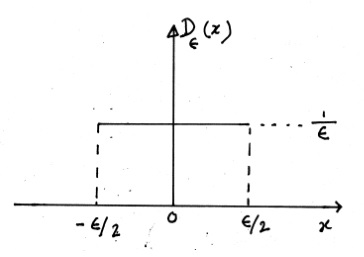
\includegraphics[width=80mm]{rep1.jpg}
\caption{Plot of the function defined in Eq. (\ref{eq:rep1})}
\end{figure}

\noindent
The integral of the function with respect to $x$ is unity, i.e.,
\be
\int_{-\infty}^{\infty} D_{\epsilon}(x) dx =1.
\ee
Now, imagine making $\epsilon$ smaller. As we decrease $\epsilon$, the function gets narrower and taller, but the integral
of the function (i.e., the area under the graph of the function) remains constant at the value 1. In the limit
$\epsilon \rightarrow 0$, the function $D_{\epsilon}(x)$ collapses to a single point, namely $x=0$, and gets infinitely tall. So,
$\lim_{\epsilon\rightarrow 0}D_{\epsilon}(x)$ is not a function at all and the procedure of taking the limit
$\epsilon \rightarrow 0$ is not justified.

\paragraph{}
However, we can make the limiting procedure meaningful if we multiply $D_{\epsilon}(x)$ by some well-defined function
$f(x)$, integrate over $x$ and then take the limit $\epsilon \rightarrow 0$. Consider the integral
\[ \int_{-\infty}^{\infty} D_{\epsilon}(x)f(x)dx \]
where $f(x)$ is a well-defined function. If $\epsilon$ is sufficiently small, the variation of $f(x)$ over the effective
integration interval $[-\epsilon/2,\epsilon/2]$ is negligible and $f(x)$ remains practically equal to $f(0)$. Therefore,
\be
\int_{-\infty}^{\infty} D_{\epsilon}(x)f(x) dx \approx f(0) \int_{-\infty}^{\infty} D_{\epsilon}(x)dx = f(0).
\ee
The smaller the value of $\epsilon$, the better the approximation. In the limit $\epsilon \rightarrow 0$, the above equation is exact:
\be
\lim_{\epsilon \rightarrow 0}\int_{-\infty}^{\infty}D_{\epsilon}(x)f(x)dx = f(0).
\ee
Now, we define the Dirac Delta Function $\delta(x)$ as
\be
\int_{-\infty}^{\infty}\delta(x) f(x)dx \stackrel{{\rm def}}= \lim_{\epsilon \rightarrow 0}\int_{-\infty}^{\infty}D_{\epsilon}(x)f(x)dx = f(0)
\ee
This equation is valid for any function $f(x)$  defined at the origin. More generally, $\delta(x-x_0)$ is defined as
\be
\int_{-\infty}^{\infty} \delta(x-x_0)f(x)dx = f(x_0).
\ee

\paragraph{}
Actually, the integral notation
\[ \int_{-\infty}^{\infty}\delta(x)f(x)dx\]
is not justified because $\delta(x)$ is not really a function. Physically, there is no problem since it becomes impossible to distinguish
between $D_{\epsilon}(x)$ and $\delta(x)$ as soon as $\epsilon$ becomes negligible compared to all distances involved in a physical problem.
Whenever a mathematical difficulty might arise, all we need to do is to assume that $\delta(x)$ is actually $D_{\epsilon}(x)$ with
$\epsilon$ extremely small but not strictly zero.

\paragraph{}
Formally, we can express $\delta(x)$ as a limit of a sequence of proper functions:
\be
\lim_{\epsilon \rightarrow 0}D_{\epsilon}(x) \equiv \delta(x).
\ee
Here $D_{\epsilon}(x)$, which is a proper function of $x$, is called the representation of the delta function. The representation we have discussed so far is the ``square function" given in Eq. (\ref{eq:rep1}). The representation is not unique. There are other functions which 
approach the delta function when appropriate limits are taken.

\subsubsection{\underline{Gaussian Representation}}
Consider the function
\be
D_{\epsilon}(x) =\frac{1}{\epsilon \sqrt{\pi}}e^{-x^2/\epsilon^2} \;\; (\epsilon>0).
\label{eq:rep2}
\ee
For each value of the parameter $\epsilon$, this function satisfies
\be
\int_{-\infty}^{\infty}D_{\epsilon}(x) dx =1.
\ee
This  is the normalized Gaussian function whose plot is shown in the figure below.
\begin{figure}[ht]
\centering
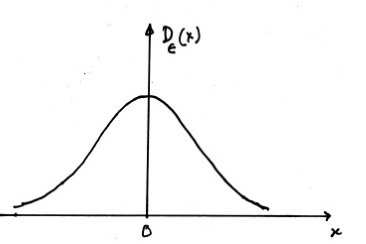
\includegraphics[width=80 mm]{rep2.jpg}
\caption{Plot of the Gaussian function defined in Eq. (\ref{eq:rep2})}
\end{figure}

\noindent
The Gaussian function has a peak at the origin. The peak has a height $1/\epsilon\sqrt{\pi}$ and a width of order $\epsilon$
(exactly how the width is defined doesn't matter). So if $\epsilon$ is allowed to be very small, the peak becomes very tall and very 
narrow. Outside the peak the function becomes extremely small. Thus we have
\be
\delta(x) = \lim_{\epsilon \rightarrow 0} \frac{1}{\epsilon \sqrt{\pi}} e^{-x^2/\epsilon^2}.
\ee

\vspace{10 mm}
\noindent
{\bf Mathematical Notes:} \newline
\noindent
We have the integral
\[ \int_{-\infty}^{\infty}e^{-x^2}dx = \sqrt{\pi}. \]
Now let us consider the following integral
\[ I= \int_{-\infty}^{\infty}e^{-b^2x^2+ a x}dx.\]
First, write
\[ b^2x^2+ax = \left(bx+\frac{a}{2b}\right)^2-\frac{a^2}{4b^2} .\]
Therefore,
\begin{eqnarray*}
I & =& e^{a^2/4b^2}\int_{-\infty}^{\infty}e^{-(bx+a/2b)^2}dx \\
& = & e^{a^2/4b^2}(1/b)\int_{-\infty}^{\infty}e^{-z^2}dz \quad (z=bx+\frac{a}{2b}) \\
& = & e^{a^2/4b^2}\frac{\sqrt{\pi}}{b}.
\end{eqnarray*}

\subsubsection{\underline{Damped Sinusoidal Representation of the Delta Function}}
Consider another function
\be
D_{\epsilon}(x) = \frac{1}{\pi}\, \frac{\sin (x/\epsilon)}{x}\quad (\epsilon > 0).
\label{eq:rep3}
\ee
A plot of the function is shown below.
\begin{figure}[ht]
\centering
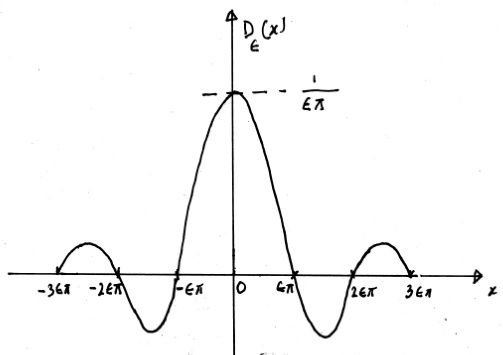
\includegraphics[width=100 mm]{rep3.jpg}
\caption{Plot of the function defined in Eq. (\ref{eq:rep3})}
\end{figure}
The function $D_{\epsilon}(x)$ has the value $1/\epsilon\sqrt{\pi}$ at $x=0$ and it oscillates with decreasing amplitude
as $|x|$ increases. The width of the central maximum is of the order of $\epsilon$ and the period of oscillations with respect to
$x$ is $2\pi \epsilon$.



\noindent
For any value of $\epsilon$ we have
\be
\int_{-\infty}^{\infty} D_{\epsilon}(x)dx = 1.
\ee


\paragraph{}
Thus, the limit of the function as $\epsilon \rightarrow 0$ has all the properties of the delta function: it becomes infinitely large
at $x=0$, and infinitely rapid oscillations as $|x|$ increases means that the entire contribution to an integral containing this
function comes from an infinitesimal neighborhood of $x=0$. We can therefore write
\be
\delta(x) = \lim_{\epsilon \rightarrow 0} \frac{1}{\pi}\, \frac{\sin(x/\epsilon)}{x}
\ee

\vspace{10 mm}
\subsubsection{\underline{Other representation of the Delta Function}}
We can also show that
\begin{eqnarray}
\delta(x) &=& \lim_{\epsilon \rightarrow 0} \frac{1}{2\epsilon}\, e^{-|x|/\epsilon} \\
\delta(x) &=& \lim_{\epsilon \rightarrow 0} \frac{1}{\pi}\, \frac{\epsilon}{x^2+\epsilon^2} \\
\delta(x) &=& \lim_{\epsilon \rightarrow 0} \frac{\epsilon}{\pi}\, \frac{\sin^2(x/\epsilon)}{x^2}.
\end{eqnarray}



\section{Properties of the Delta Function}
It is important to note that, because of its singular character, the $\delta$-function cannot be the end result of a calculation,
and has meaning only so long as a subsequent integral over its argument is carried out. With this understanding we can write
down some relations between delta functions:
\begin{enumerate}
\item
The delta function is an even function, i.e.,
\be
\delta(-x)=\delta(x).
\ee

\item
\be
x\delta(x)=0.
\ee

\item
\be
\delta(ax) = \frac{1}{|a|} \delta(x).
\ee
{\bf Proof:}\newline
Consider the integral
\[
I=\int_{-\infty}^{\infty}\delta(ax)f(x)dx. 
\]
Since the delta function is an even function it doesn't matter if we replace $a$ by $|a|$ in the argument. Thus
\[ I= \int_{-\infty}^{\infty} \delta(|a|x)f(x) dx \, . \]
Making the change of variable
\[ y=|a|x \]
we have
\[ I= \frac{1}{|a|} \int_{-\infty}^{\infty} \delta(y)f(y/|a|) dy= \frac{1}{|a|} f(0) \, , \]
or,
\[ \int_{-\infty}^{\infty} \delta(ax)f(x) dx  = \frac{1}{|a|} \int_{-\infty}^{\infty} \delta(x)f(x) dx \, , \]
i.e.,
\begin{equation*}
\boxed{
\delta(ax)=\frac{1}{|a|}\delta(x)
}
\end{equation*}

\item
More generally, we have
\be
\delta(\phi(x)) = \sum_i \frac{\delta(x-x_i)}{\left|\frac{\partial\phi}{\partial x}\right|_{x_i}}
\ee
where the sum runs over the $x_i$'s which are the simple roots of $\phi(x)$.

\noindent
{\bf Proof:}\newline
Let $x_1, x_2, \cdots , x_N$ be the simple roots of $\phi(x)$ (figure below):
\begin{figure}[ht]
\centering
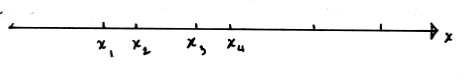
\includegraphics[width=80 mm]{roots.jpg}
\caption{Simple roots of $\phi(x)$.}
\end{figure}

\noindent
In the neighborhood of any of the simple roots $x_i$, we can write
\[ \phi(x) = (x-x_i)\psi(x) \]
where $\psi(x_i) \neq 0$. We have
\[ \psi(x_i) = \left. \frac{\partial \phi(x)}{\partial x}\right|_{x=x_i}. \]

Now, consider the integral
\begin{eqnarray*}
\int_{-\infty}^{\infty} \delta(\phi(x))f(x)dx &=& \sum_{i=1}^N\int_{x_i-\epsilon}^{x_i+\epsilon}
\delta\left[(x-x_i)\psi(x_i)\right]f(x)dx \\
& = & \sum_{i=1}^N  \frac{1}{|\psi(x_i)|}  \int_{x_i-\epsilon}^{x_i+\epsilon} \delta(x-x_i)f(x)dx \\
& = & \sum_{i=1}^N\frac{1}{|\frac{\partial \phi}{\partial x}|_{x=x_i}}  \int_{-\infty}^{\infty} \delta(x-x_i)f(x)dx \\
& = & \sum_{i=1}^N\frac{1}{|\frac{\partial \phi}{\partial x}|_{x=x_i}}  f(x_i) 
\end{eqnarray*}
The above result is obtained if we write
\be
\delta(\phi(x)) = \sum_{i=1}^N \frac{\delta(x-x_i)}{~~\left| \frac{\partial \phi}{\partial x} \right|_{x=x_i} }. \quad {\rm Proved.}
\ee

\item
A frequently used example of the above result is
\be
\delta(x^2-a^2) = \frac{1}{2a}\delta(x-a) + \frac{1}{2a}\delta(x+a), \;\;\; (a>0).
\ee
Here
\[ \phi(x) = x^2-a^2 = (x-a)(x+a). \]
The two simple roots of $\phi(x)$ are at $x=a$ and $x=-a$. Now
\[ \left| \frac{\partial \phi}{\partial x}\right|_{x=a} = |2x|_{x=a} = 2a \]
and
\[ \left| \frac{\partial \phi}{\partial x}\right|_{x=-a} = |2x|_{x=-a} = 2a .\]
Therefore, the above result follows.

\item
\[ f(x)\delta(x-a) = f(a)\delta(x-a).\]

\item
\[ \int \delta(x-y)\delta(y-a) dy = \delta(x-a). \]

\end{enumerate}

\noindent
{\bf Note 1:}\newline
We have the identity
\[ x\delta(x) = 0. \]
The converse is also true and it can be shown that the equation
\[ xu(x)=0 \]
has the general solution
\[ u(x) = c \delta(x).\]

\vspace{10 mm}
\noindent {\bf Note 2:}\newline
We will now prove an identity which is particularly useful in quantum mechanics:
\be
\lim_{\epsilon \rightarrow 0^+} \int_{-\infty}^{\infty} \frac{1}{x \pm  i\epsilon}\, f(x)dx =
\mathcal{P} \int_{-\infty}^{\infty}\frac{dx}{x} f(x)  \mp i\pi f(0),
\ee
or, in short 
\be
\lim_{\epsilon \rightarrow 0^+} \frac{1}{x\pm i\epsilon} = \mathcal{P} \left( \frac{1}{x} \right) \mp i\pi \delta(x),
\ee
where it is understood that the second of these two equations have meaning only within an integral. The symbol $\mathcal{P}$
means the the principal part of an integral where the integrand has a simple pole. The principal part is defined as
\be
\mathcal{P} \int_{-A}^{B} \frac{dx}{x} f(x) = \lim_{\eta \rightarrow 0^+}\left[ \int_{-A}^{-\eta} + \int_{\eta}^B\right]
\frac{dx}{x} f(x).
\ee

\noindent
{\bf Proof:}\newline
We can write
\be
\frac{1}{x\pm i\epsilon} = \frac{x\mp i\epsilon}{x^2+\epsilon^2}= \frac{x}{x^2+\epsilon^2} \mp \frac{i\epsilon}{x^2+a^2}.
\label{eq:pv1}
\ee
Now, we have
\[ \lim_{\epsilon \rightarrow 0^+} \frac{1}{\pi}\, \frac{\epsilon}{x^2+ \epsilon^2} = \delta(x). \]
Therefore,
\be
\lim_{\epsilon \rightarrow 0^+} (\mp) i \frac{\epsilon}{x^2+a^2} = \mp i\pi \delta(x).
\ee
Next, consider the first term on the right and side of Eq. (\ref{eq:pv1}). We multiply this term by a function $f(x)$ which is regular 
at the origin and then integrate over $x$. We get

\begin{multline}
\lim_{\epsilon \rightarrow 0^+} \int_{-\infty}^{\infty}\frac{xf(x)}{x^2+a^2} dx \\
= \lim_{\epsilon \rightarrow 0^+} \left[ \lim_{\eta \rightarrow 0^+} \int_{-\infty}^{-\eta}\frac{xf(x)}{x^2+a^2} dx 
+ \lim_{\eta \rightarrow 0^+} \int_{-\eta}^{\eta}\frac{xf(x)}{x^2+a^2} dx 
+ \lim_{\eta \rightarrow 0^+} \int_{\eta}^{\infty}\frac{xf(x)}{x^2+a^2} dx \right]
\label{eq:pv2}
\end{multline}
Note that we take the limit over $\eta$ first and the we take the limit over $\eta$. Now consider the second integral of the above equation.
\[
\lim_{\eta \rightarrow 0^+} \int_{-\eta}^{\eta}\frac{xf(x)}{x^2+a^2} dx= f(0) \lim_{~\eta \rightarrow 0^+}
\frac{1}{2} \left[ \ln (x^2+ \epsilon^2) \right]_{x=-\eta}^{x=\eta} = 0.
\]
If we now reverse the order of the evaluation of limits in Eq. (\ref{eq:pv2}), the $\epsilon \rightarrow 0^+$ limit
causes no difficulties in the other two integrals. We thus have
\begin{eqnarray*}
\lim_{\epsilon \rightarrow 0^+} \int_{-\infty}^{\infty}\frac{xdx}{x^2+a^2}f(x) &=& \lim_{\eta \rightarrow 0^+}
\lim_{\epsilon \rightarrow 0^+}\left[ \int_{-\infty}^{-\eta} + \int_{\eta}^{\infty}\right] \frac{xdx}{x^2+a^2}f(x) \\
&=& \lim_{\eta \rightarrow 0^+} \left[ \int_{-\infty}^{-\eta} + \int_{\eta}^{\infty}\right] \frac{dx}{x}f(x)\\
&=& \mathcal{P}  \int_{-\infty}^{\infty} \frac{1}{x} f(x)dx
\end{eqnarray*}
This establishes the identity.


\section{Derivative of the Delta Function}
One may define the derivative $\delta^{\prime}(x)$ of the delta function. When $\epsilon$ is small, the derivative of 
$D_{\epsilon}(x)$ has two peaks close to the origin, one peak being positive and the other negative as shown in the figure
below.
\begin{figure}[ht]
\centering
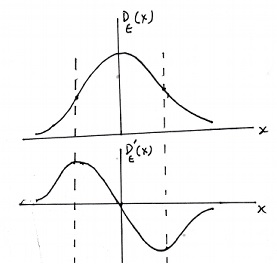
\includegraphics[width=90 mm]{derivative.jpg}
\caption{Plot of $D_{\epsilon}(x)$ and $D^{\prime}_{\epsilon}(x)$.}
\end{figure}


\noindent
As $\epsilon \rightarrow 0$, each of the peaks become very narrow and very tall, and each of the two peaks approach very close to the
origin.  Now, an integration by parts gives
\be
\int_{-\infty}^{\infty} D_{\epsilon}^{\prime}(x)f(x) dx = \left[ D_{\epsilon}(x)f(x)\right]_{-\infty}^{\infty}
- \int_{-\infty}^{\infty} D_{\epsilon}(x) f^{\prime}(x) dx\, . 
\ee
Because $D_{\epsilon}(x)$ tends to zero as $x \rightarrow \pm \infty$, the first term on the right hand side vanishes unless
$f(x)$ explodes violently at infinity. So by letting $\epsilon \rightarrow 0$, we arrive at the definition of
$\delta^{\prime}(x)$:
\be
\boxed{
\int_{-\infty}^{\infty} \delta^{\prime}(x) f(x) dx = - \int_{-\infty}^{\infty}\delta(x)f^{\prime}(x) dx = -f^{\prime}(0).
}
\label{eq:deltaprime}
\ee
From this we immediately get 
\be
\boxed{
x\delta^{\prime}(x) =-\delta(x).
}
\ee
Conversely, it can be shown that the general solution of the equation
\[ xu(x) = \delta(x) \]
can be written as
\[ u(x) =-\delta^{\prime}(x) + c \delta(x) \]
where the second term arises from the homogeneous equation
\[ x\delta(x) = 0. \]
From the definition (\ref{eq:deltaprime}) it also follows that
\be
\boxed{
\delta^{\prime}(-x) = - \delta^{\prime}(x).
}
\ee
The $n^{th}$ order derivative of $\delta(x)$ can be defined in the same way. We find
\be
\int_{-\infty}^{\infty} \delta^{(n)}(x) f(x) dx = (-1)^n f^{(n)}(0).
\ee
We can also prove the following properties of the derivatives of the delta function:
\begin{eqnarray*}
\delta^{(m)}(x)& = &(-1)^m \delta^{(m)}(-x)  \\
x^{m+1}\delta^{(m)}(x)& = & 0  \\
x \delta^{(m)}(x)& = &-(m-1) \delta^{(m-1)}(x).
\end{eqnarray*}


\section{Integration of the Delta Function}
Consider the indefinite integral
\be
\theta_{\epsilon}(x) = \int_{-\infty}^x D_{\epsilon}(y)dy .
\label{eq:theta}
\ee
A graph of $\theta_{\epsilon}(x)$ versus $x$ is shown below.
\begin{figure}[ht]
\centering
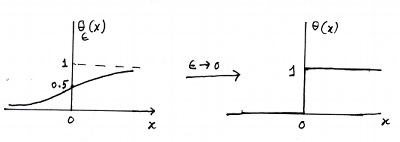
\includegraphics[width=\linewidth]{theta.jpg}
\caption{The $\theta$-function as an integral of the delta function}
\end{figure}


\noindent
As $\epsilon \rightarrow 0$, the step in the function $\theta_{\epsilon}(x)$ gets progressively steeper, until, finally, the function changes abruptly from 0 to 1 at $x=0$. Therefore, taking the limit $\epsilon \rightarrow 0$ in Eq. (\ref{eq:theta})
we have
\be
\theta(x) = \int_{-\infty}^x\delta(y)dy
\label{eq:theta2}
\ee
where
\be
\theta(x) = \left\{ \begin{array}{cl}
                     1 & {\rm for}\; x>0 \\
										0 & {\rm for}\; x<0.
										\end{array} \right.
\ee										
If we differentiate Eq. (\ref{eq:theta2}) with respect to $x$, we get
\be
\frac{d\theta(x)}{dx} = \delta(x).
\ee


\section{Three dimensional delta function}
The three-dimensional delta function $\delta(\vec{r}\,)$ is defined as
\be
\delta(\vec{r}\,) \stackrel{{\rm def}} \equiv \delta(x) \delta(y) \delta(z).
\ee
In other words, $\delta(\vec{r}\,)$ is zero if any of the coordinates $x$, $y$ and $z$ is {\underline{not}} equal to 
zero and $\delta(\vec{r}\,)$ tends to infinity at the origin, i.e., when $x=0$, $y=0$ and $z=0$, such that
\be
\int_{{\rm volume}}\delta(\vec{r}\,)d^3r = 1
\ee
if the volume of integration contains the origin. We also have
 \be
\int \delta(\vec{r}\,)f(\vec{r}\,)d^3r = f(0)
\ee
where again the volume of integration contains the origin. 

\vspace{10 mm}
\noindent
{\bf Note:}
\begin{itemize}
\item
$\delta(\vec{r} - \vec{r}^{\;\prime}\, ) = \delta(x-x^{\prime})\delta(y-y^{\prime})\delta(z-z^{\prime})$
\item $ \int_{V} \delta(\vec{r} - \vec{r}^{\;\prime}\, )d^3r =1 $
\newline
where the volume of integration includes the point $\vec{r}^{\;\prime}$. Otherwise, the integral is zero.
\item $ \int_{V} \delta(\vec{r} - \vec{r}^{\;\prime}\, ) f(\vec{r}\,)d^3r = f(\vec{r}^{\; \prime})$ \newline
if $V$ includes the point $\vec{r}^{\;\prime}$.

\end{itemize}



\subsubsection{A useful formula}
Consider the integral
\begin{eqnarray*}
\int_{-\infty}^{\infty}e^{ikx} dx &=& \lim_{L\rightarrow \infty} \int_{-L}^{L} e^{ikx}dx \\
&=& \lim_{L\rightarrow \infty} \frac{1}{ik}\, \left(e^{ikL}-e^{-ikL} \right) \\
&=& \lim_{L\rightarrow \infty} \, \frac{2}{k} \left( \frac{ e^{ikL}-e^{-ikL}}{2i} \right) \\
&=& \lim_{L\rightarrow \infty}\, \frac{2}{k}\sin kL \\
&=& 2\pi \lim_{L\rightarrow \infty}\, \frac{\sin kL}{\pi k}\\
&=& 2\pi \delta(k),
\end{eqnarray*}
where we have used
\be
\lim_{\epsilon \rightarrow 0} \frac{ \sin (x/\epsilon)}{\pi x} = \delta(x).
\ee
Thus, we have the very important formula
\be
\boxed{
\int_{-\infty}^{\infty}e^{ikx}dx = 2\pi \delta(k)
}
\label{eq:ft3}
\ee
In Eq. (\ref{eq:ft3}) if we integrate with respect to $k$, we would have $\delta(x)$ on the right hand side,
\be
\boxed{
\int_{-\infty}^{\infty}e^{ikx}dk = 2\pi \delta(x)
}
\label{eq:ft4}
\ee
Also note that in Eq. (\ref{eq:ft3}) we integrate over the full domain of $x$ from $-\infty$ to $\infty$. Making a change of variable $x\rightarrow -x$ does not change the value of the integral. Hence we also have
\be
\boxed{
\int_{-\infty}^{\infty}e^{-ikx}dx = 2\pi \delta(k)
}
\label{eq:ft5}
\ee
Similarly, in Eq. (\ref{eq:ft4}), making the change of variable $k \rightarrow -k$, doesn't change the value of the integral. So we could also write
\be
\boxed{
\int_{-\infty}^{\infty}e^{-ikx}dk = 2\pi \delta(x)
}
\label{eq:ft6}
\ee
Thus, in summary
\be
\int_{-\infty}^{\infty}e^{\pm ikx}dx = 2\pi \delta(k),
\ee
and
\be
\int_{-\infty}^{\infty}e^{\pm ikx}dk = 2\pi \delta(x),
\ee
In three dimensions we have
\be
\int_{{\rm all\; space}}e^{\pm i\vec{k}.\vec{r}}d^3r = (2\pi)^3 \delta(\vec{k}\,).
\ee
\be
\int_{{\rm all\; space}}e^{\pm i(\vec{k}-\vec{k}^{\;\prime}).\vec{r}}d^3r = (2\pi)^3 \delta(\vec{k}-\vec{k}^{\;\prime}\,).
\ee
\be
\int_{{\rm all\; space}}e^{\pm i \vec{k}.(\vec{r}-\vec{r}^{\;\prime})}d^3k = (2\pi)^3 \delta(\vec{r}-\vec{r}^{\;\prime}\,).\ee


\section{Fourier transform}

We can always express a function $f(x)$ in the form
\be
f(x) = \int_{-\infty}^{\infty}e^{ikx}\tilde{f}(k)dk
\label{eq:ft10}
\ee
where $\tilde{f}(k)$ is a function of $k$, called the Fourier transform of $f(x)$. From Eq. (\ref{eq:ft10}) we can write
\begin{eqnarray*}
\int_{-\infty}^{\infty}e^{-ik^{\prime}x}f(x)dx &=& \int_{-\infty}^{\infty}\int_{-\infty}^{\infty}e^{i(k-k^{\prime}\,)x}
\tilde{f}(k)dkdx \\
&=& 2\pi \int_{-\infty}^{\infty}\delta(k-k^{\prime}\,)\tilde{f}(k)dk \\
&=& 2\pi \tilde{f}(k^{\prime}\,)
\end{eqnarray*}
Thus, 
\be
\tilde{f}(k) = \frac{1}{2\pi}\int_{\infty}^{\infty}e^{-ikx}f(x)dx.
\label{eq:ft11}
\ee
The functions $f(x)$ and $\tilde{f}(k)$ are Fourier transform of each other. We can write Eqs. (\ref{eq:ft10}) 
and (\ref{eq:ft11}) in a more symmetrical fashion as follows
\begin{eqnarray}
f(x)& = &\frac{1}{\sqrt{2\pi}} \int_{-\infty}^{\infty}e^{ikx}\tilde{f}(k)dk \\
\tilde{f}(k) &=& \frac{1}{\sqrt{2\pi}}\int_{\infty}^{\infty}e^{-ikx}f(x)dx.
\end{eqnarray}

\paragraph{}
In three dimensions we can write
\be
f(\vec{r}\,) = \frac{1}{(2\pi)^{3/2}} \int e^{i\vec{k}.\vec{r}} \tilde{f}(\vec{k}\,)d^3k.
\ee
Multiplying this equation by $e^{-i\vec{k}^{\; \prime}.\vec{r}}$ and integrating over $\vec{r}$, we have
\begin{eqnarray*}
\int_{{\rm all\; space}} e^{-i\vec{k}^{\; \prime}.\vec{r}} f(\vec{r}\,)d^3r
&=& \frac{1}{(2\pi)^{3/2}} \int d^3r\int d^3k\, e^{i(\vec{k}-\vec{k}^{\; \prime}).\vec{r}}\tilde{f}(\vec{k}\,) \\
&=& \frac{1}{(2\pi)^{3/2}} \int d^3k\, (2\pi)^{3} \delta(\vec{k}-\vec{k}^{\; \prime})\tilde{f}(\vec{k}\,) \\
&=& (2\pi)^{3/2} \tilde{f}(\vec{k}^{\; \prime}\,)
\end{eqnarray*}
Therefore,
\be
\tilde{f}(\vec{k}\,) = \frac{1}{(2\pi)^{3/2}}\int e^{-i\vec{k}.\vec{r}} f(\vec{r}\,)d^3r.
\ee


\noindent
In summary, 

\begin{eqnarray}
f(\vec{r}\,)& =& \frac{1}{(2\pi)^{3/2}} \int e^{i\vec{k}.\vec{r}} \tilde{f}(\vec{k}\,)d^3k, \\
\tilde{f}(\vec{k}\,)& =& \frac{1}{(2\pi)^{3/2}}\int e^{-i\vec{k}.\vec{r}} f(\vec{r}\,)d^3r.
\end{eqnarray}


\newpage

\subsection{Parseval Identity}
We will now prove the important identity
\be
\int \left|f(\vec{r}\,)\right|^2d^3r = \int \left| \tilde{f}(\vec{k}\,)\right|^2d^3k.
\ee

\vspace{5 mm}
{\bf \underline{Proof}:}
\begin{multline}
\int \left|f(\vec{r}\,)\right|^2d^3r = \int f(\vec{r}\,) f^*(\vec{r}\,)d^3r \\
=\int d^3r \, \frac{1}{(2\pi)^{3/2}} \int e^{i\vec{k}.\vec{r}} \tilde{f}(\vec{k}\,)d^3k \,
\frac{1}{(2\pi)^{3/2}}   \int e^{-i\vec{k}^{\; \prime}.\vec{r}} \tilde{f}^*(\vec{k}^{\; \prime}\,)d^3k^{\prime}~~~~\\
=\frac{1}{(2\pi)^3}\int d^3k d^3k' \tilde{f}(\vec{k}\,) \tilde{f}^*(\vec{k}^{\; \prime}\,)
\underbrace{ \int d^3r\, e^{i(\vec{k}-\vec{k}^{\; \prime}\,).\vec{r}} }_{(2\pi)^3 \delta(\vec{k}-\vec{k}^{\; \prime}\,) }
\qquad \qquad \qquad ~~~\\
= \int d^3k d^3k' \tilde{f}(\vec{k}\,) \tilde{f}^*(\vec{k}^{\; \prime}\,)\delta(\vec{k}-\vec{k}^{\; \prime}\,) \qquad
\qquad \qquad \qquad \qquad ~~~~~~\\
= \int d^3k  \tilde{f}(\vec{k}\,) \tilde{f}^*(\vec{k}\,) \qquad \qquad \qquad \qquad \qquad\qquad\qquad\qquad
~~~~~ \\
= \int d^3k \left | \tilde{f}(\vec{k}\,) \right|^2. \qquad \qquad \qquad \qquad \qquad \qquad \qquad \qquad \qquad ~~
\end{multline}

The proof is now complete.


					







\begin{titlepage}
\begin{center}
        
\vspace*{5cm}
        
\Huge
\textbf{DIRAC DELTA FUNCTION \\ FOR \\ STUDENTS IN A HURRY}

\vspace*{1cm}

\large
\textbf{\textit{by}}

\vspace*{1cm}
\Large
\textbf{Prof. Dr. Khorshed Ahmed Kabir}

\end{center}

\end{titlepage}



\section*{Dirac Delta Function}
Consider the function $D_\epsilon (x)$ given by 
\begin{align*}
D_\epsilon (x) & = \frac{1}{\epsilon} \ \ ;\ for -\frac{\epsilon}{2} \leq x \leq \frac{\epsilon}{2} \\
& = 0 \ \ \ ;\ for \ |x| > \frac{\epsilon}{2}
\end{align*}
where $\epsilon$ is a positive parameter. The plot of the function is shown below.

\vspace{0.2cm}
\begin{center}
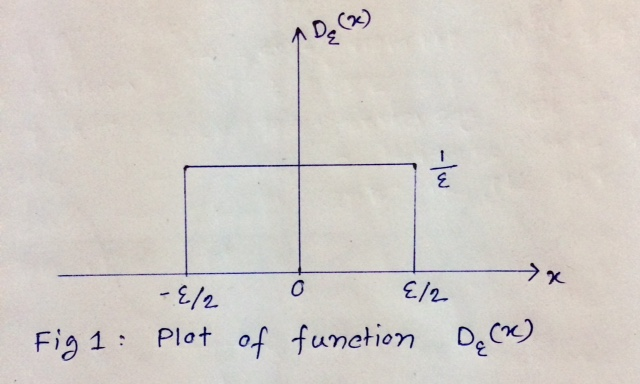
\includegraphics[width=0.5\textwidth]{DiracDeltaFig1.jpg}
\end{center}

The integral of the function with respect to x is 1, i.e,
\begin{equation}
\int_{-\infty}^\infty D_\epsilon (x) dx = 1 
\end{equation}

Now imagine making $\epsilon$ smaller. As we decrease $\epsilon$, the function gets narrower and taller, but the integral of the function i.e, the area under the graph remain constant at the value 1. In the limit $\epsilon \to 0$, the function $D_{\epsilon} (x)$ collapses to a single point $x=0$ and gets infinitely tall. So, $\lim_{\epsilon \to 0} D_\epsilon (x)$ is not a function at all and the procedure of taking the limit $\epsilon \to 0$ is not justified.\\

However, we can make the limiting procedure meaningful if multiply $D_\epsilon (x)$ by some well defined function $f(x)$, integrate over x and then take the limit $\epsilon \to 0$. Consider, the integral $$\int_{-\infty}^\infty D_\epsilon (x) f(x) dx $$ where $f(x)$ is a well defined function. If $\epsilon$ is significantly small, the variation of $f(x)$ over the effective integration interval $[-\frac{\epsilon}{2},\frac{\epsilon}{2}]$ is negligible and $f(x)$ remain practically equal to f(0). Therefore,
\begin{equation}
\int_{-\infty}^{\infty} D_\epsilon (x) f(x) dx \ \simeq f(0) \int_{-\infty}^{\infty} D_\epsilon (x) dx = f(0)
\end{equation}
The smaller the value of $\epsilon$, the better the approximation. in the limit $\epsilon \to 0$, the above equation is exactly
\begin{equation}
\lim_{\epsilon \to 0} \int_{-\infty}^{\infty} D_\epsilon (x) f(x) dx = f(0)
\end{equation} 
Now, we define the delta function by the relation
\begin{equation}
\int_{-\infty}^\infty \delta (x) f(x) dx = \lim_{\epsilon \to 0} \int_{-\infty}^{\infty} D_\epsilon (x) f(x) dx = f(0)
\end{equation}
This equation is valid for any function defined at the origin. More generally, $\delta (x-x_0)$ is defined as
\begin{equation}
\int_{-\infty}^\infty \delta (x-x_0) f(x) dx = f(x_0)
\end{equation}
Actually, the integral notation $\int_{-\infty}^\infty \delta (x) f(x) dx $ is not justified because $\delta(x)$ is not really a function. Physically, there is no problem since it becomes impossible to distinguish between $D_\epsilon (x)$ and $\delta (x)$ as soon as $\epsilon$ becomes negligible compared to all the distances involved in a physical problem. Whenever a mathematical difficulty arise, all we need to do is to assume that $\delta (x)$ is actually $D_\epsilon (x)$ with $\epsilon$ extemely small but not strictly zero.\\

Formally, we can express $\delta(x)$ as a sequence of proper functions $$\lim_{\epsilon \to 0} D_\epsilon (x) \equiv \delta(x) $$ Here, $D_\epsilon (x)$, which is a proper function of x is called the representation of the delta function. One representation is the 'Square Function' given at the beginning. The representation is not unique. There are other functions which approach the delta function when appropriate limits are taken.

\section*{Other Representation Of The Delta Function}
\subsection*{A}
Consider the function 
\begin{equation}
D_\epsilon (x) = \frac{1}{\epsilon \sqrt{\pi}} e^{-x^2/\epsilon^2} \ \ \ with\ \ \epsilon > 0
\end{equation}
For each value of the parameter $\epsilon$, this function satisfies $$\int_{-\infty}^\infty D_\epsilon (x)dx =1$$ 

\vspace{0.2cm}
\begin{center}
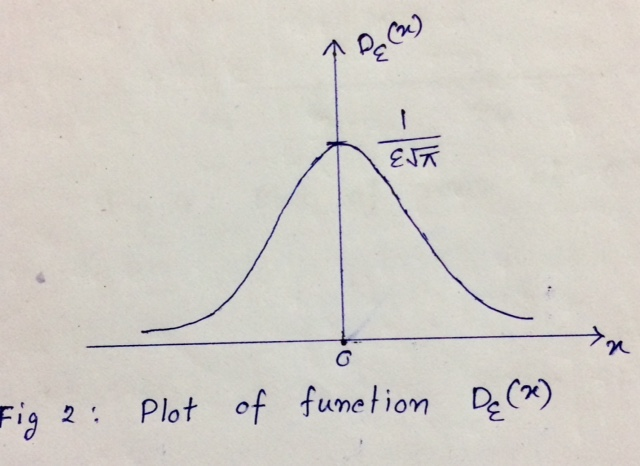
\includegraphics[width=0.5\textwidth]{DiracDeltaFig2.jpg}
\end{center}
When plotted against x, the function has a peak at the origin. The peak has a height $\frac{1}{\epsilon \sqrt{\pi}}$ and a width of order $\epsilon$ (exactly how the width is defined doesn't matter). So, if $\epsilon$ is allowed to become very small, the peak becomes very tall and very narrow. Outside the peak, the function becomes extremely small. Thus we have 
\begin{equation}
\delta (x) = \lim_{\epsilon \to 0} \frac{1}{\epsilon \sqrt{\pi}} e^{-x^2/\epsilon^2}
\end{equation}
\\\\
Note: $$\int_{-\infty}^{\infty} e^{-x^2}dx = \sqrt{\pi}$$
Let, 
\begin{align*}
I &= \int_{-\infty}^{\infty} e^{-(b^2 x^2 + ax)} dx \\
&=e^{a^2/4b^2} \int_{-\infty}^{\infty} e^{-(bx + a/2b)^2} dx \\
&= e^{a^2/4b^2} \frac{1}{b} \int_{-\infty}^{\infty} e^{-z^2} dz \\
&= e^{a^2/4b^2} \frac{\sqrt{\pi}}{b}
\end{align*}
By using $$ b^2 x^2 + ax = (bx + \frac{a}{2b})^2 - \frac{a^2}{4b^2}$$ and by letting $$ z= bx+\frac{a}{2b}$$

\subsection*{B}
Consider another function
\begin{equation}
D_{\epsilon} (x) = \frac{1}{\pi} \frac{\sin (x/\epsilon)}{x} \ \ \ with\ \epsilon>0
\end{equation}

\vspace{0.2cm}
\begin{center}
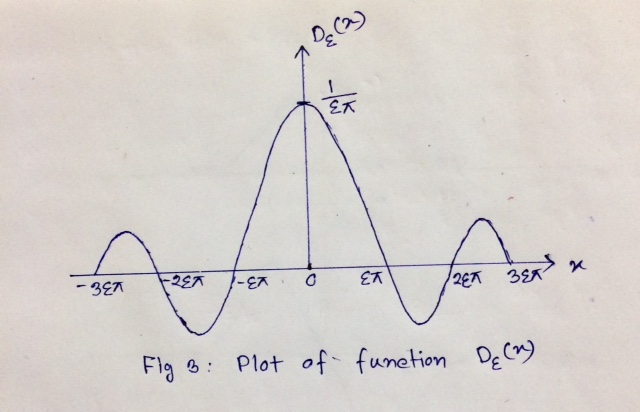
\includegraphics[width=0.6\textwidth]{DiracDeltaFig3.jpg}
\end{center}

For any value of the parameter $\epsilon$ we have 
\begin{equation}
\int_{-\infty}^{\infty} D_\epsilon (x) dx = 1
\end{equation}
A plot of the function $D_{\epsilon} (x)$ shows that it has the value $\frac{1}{\epsilon \pi}$ at x=0 and it oscillates with decreasing amplitude as $|x|$ increases. The width of the central maxima is of the order of $\epsilon$ and the period of oscillation with respect tox is $2\pi \epsilon$.

Thus the limit of the function as $\epsilon \to 0$ has all the properties of the delta function: it becomes infintely large at x=0, it has unit integral, and infinitely rapid oscillations as $|x|$ increases means that the entire contribution to an integral containing this function comes from an infinitesimal neighbourhood of x=0. We can therefore write 
\begin{equation}
\delta (x) = \lim_{\epsilon \to 0} \frac{1}{\pi} \frac{\sin (x/\epsilon)}{x}
\end{equation}

\subsection*{C}
We can also show that $$\delta (x) = \lim_{\epsilon \to 0} \frac{1}{2\epsilon} e^{-|x|/\epsilon}$$  $$\delta (x) = \lim_{\epsilon \to 0} \frac{1}{\pi} \frac{\epsilon}{x^2 + \epsilon^2}$$  $$\delta (x) = \lim_{\epsilon \to 0} \frac{\epsilon}{\pi} \frac{\sin^2 (x/\epsilon)}{x^2}$$


\section*{Properties Of The Delta Function}
It is important  to note that, because of its singular character, the delta function can not be the end result of a calculation and has meaning only so long as a subsequent integral over its argument is carried out. With this understanding we can write down some relations between delta functions.

\textbf{1.} The delta function is an even function: $$
\delta(-x) = \delta(x)$$

\textbf{2.} $$x \delta(x) = 0$$

\textbf{3.} $$\delta (ax) = \frac{1}{|a|} \delta(x) $$

\subsection*{Proof Of 3}
Consider the integral $$I = \int_{-\infty}^{\infty}\delta(ax) f(x) dx $$
Since the delta function is even in its argument, it doesn't matter if we replace a by $|a|$ in its argument. Thus $$I = \int_{-\infty}^{\infty}\delta(|a|x) f(x) dx $$.
Making the change in variable $$y=|a|x$$ we have $$I = \frac{1}{|a|} \int_{-\infty}^{\infty}\delta(y) f \left( \frac{y}{|a|} \right) dy = \frac{1}{|a|} f(0)$$
Or, $$ \int_{-\infty}^{\infty}\delta(ax) f ( x ) dx = \frac{1}{|a|} \int_{-\infty}^{\infty}\delta(x) f(x)dx$$ 
Or, $$\delta (ax) = \frac{1}{|a|}\delta(x) $$

\textbf{4.} More generally, $$\delta (\phi(x)) = \sum_i \frac{\delta(x-x_i)}{\left| \frac{\partial \phi}{\partial x} \right|_{x_i}}$$
where the sum runs over the $x_i$'s which are simple roots of $\phi(x)$.

\subsection*{Proof Of 4}
Let $x_1, x_2, x_3,..., x_N$ be the simple roots of $\phi(x)$

\vspace{0.2cm}
\begin{center}
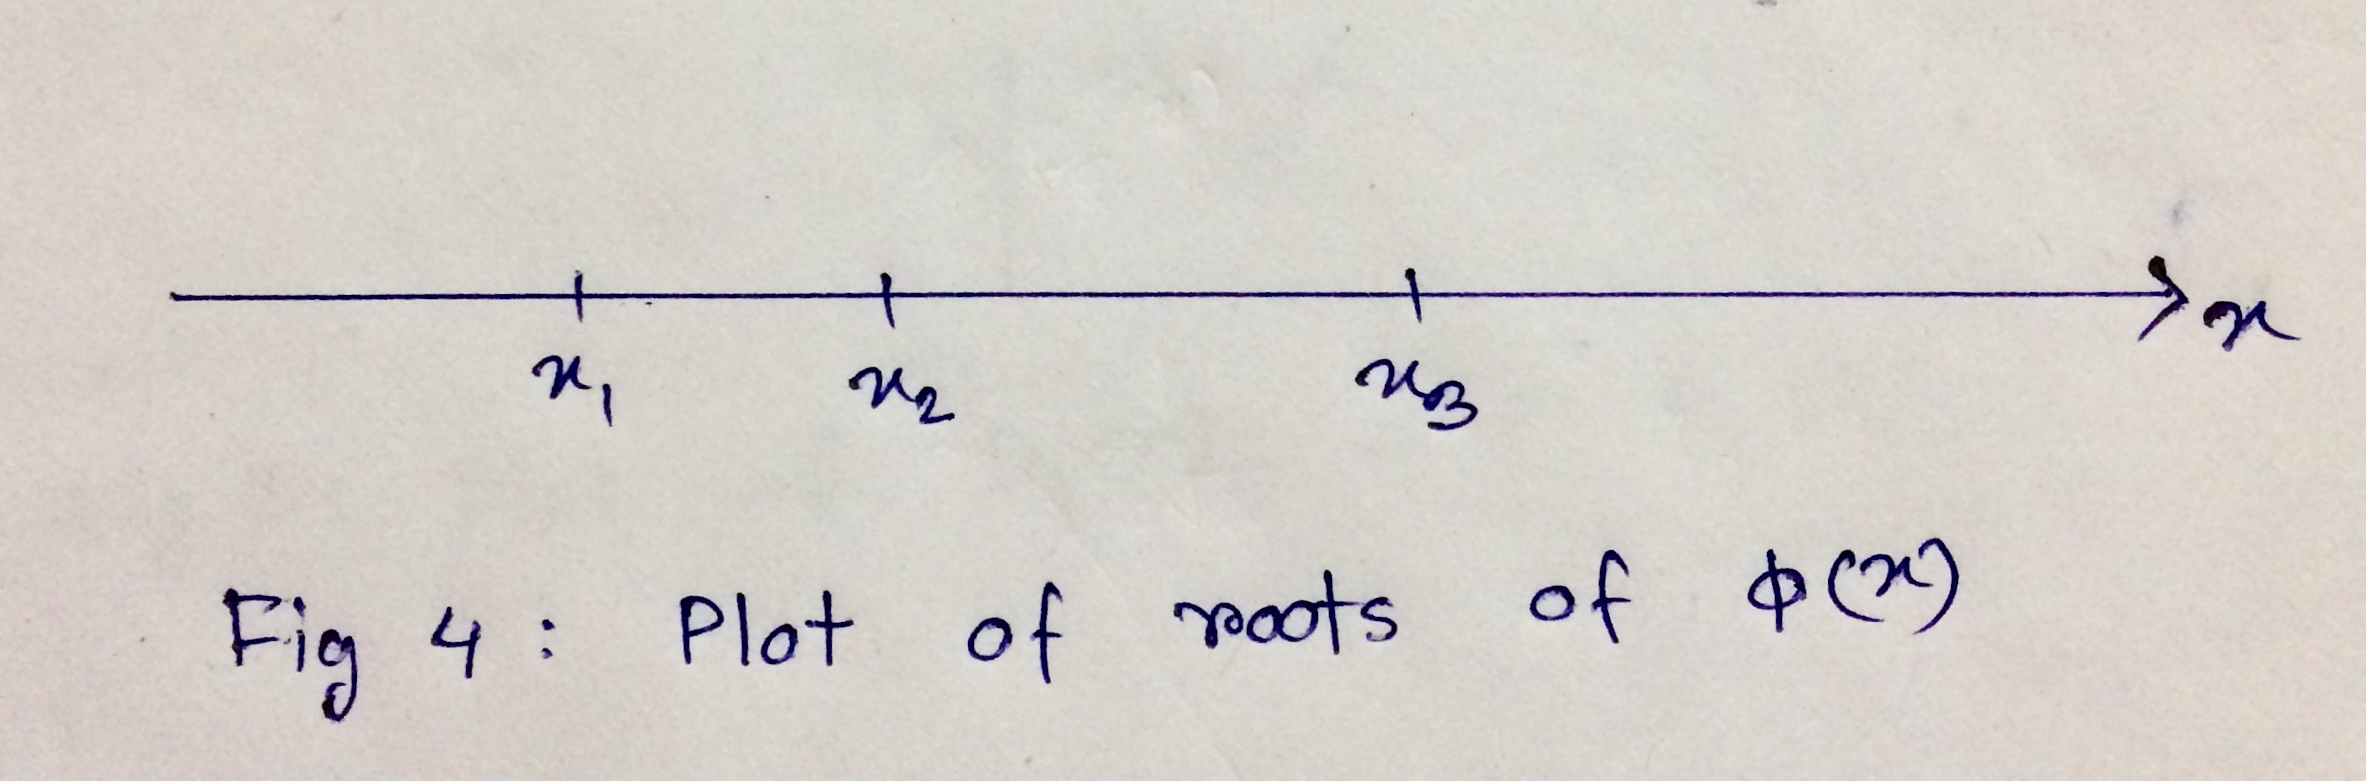
\includegraphics[width=0.6\textwidth]{DiracDeltaFig4.jpg}
\end{center}
In the neighbourhood of any one of the simple roots $x_i$, we can write $$\phi (x) = (x-x_i) \psi(x)$$ where $\psi(x_i) \neq 0$. We have $\psi (x_i) = \left. \frac{\partial \phi(x)}{\partial x} \right|_{x=x_i}$
Now consider the integral
\begin{align*}
&\ \  \int_{-\infty}^{\infty} \delta(\phi(x)) f(x) dx \\
&=\sum_{i=1}^N \int_{x_i - \epsilon}^{x_i + \epsilon} \delta[(x-x_i) \psi(x_i)] f(x) dx \\
&=\sum_{i=1}^N \frac{1}{|\psi(x_i)|} \int_{x_i - \epsilon}^{x_i + \epsilon} \delta(x-x_i) f(x) dx \\
&=\sum_{i=1}^N \frac{1}{|\frac{\partial \phi}{\partial x}|_{x=x_i}} \int_{-\infty}^{\infty} \delta(x-x_i) f(x) dx \\
&=\sum_{i=1}^N \frac{1}{|\frac{\partial \phi}{\partial x}|_{x=x_i}} f(x_i) \\
\end{align*}
The above result is obtained, if we write $$\delta (\phi (x)) = \sum_{i=1}^N \frac{\delta(x-x_i)}{\left| \frac{\partial \phi}{\partial x} \right|_{x=x_i}} $$

\textbf{5.} A frequently used example of the above result is $$\delta (x^2 - a^2) = \frac{1}{2a} \delta(x-a) + \frac{1}{2a} \delta(x+a) \ \ \ \ with a>0$$
Here $$\phi (x) = x^2 - a^2 = (x+a)(x-a)$$.
The two simple roots of $\phi(x)$ are at $x=a$ and $x=-a$. Now, $$\left| \frac{\partial \phi}{\partial x} \right|_{x=a} = |2x|_{x=a} = 2a$$ And $$\left| \frac{\partial \phi}{\partial x} \right|_{x=-a} = |2x|_{x=-a} =|-2a|= 2a$$ So, the above result follows.

\textbf{6.} $$f(x) \delta (x-a) = f(a) \delta(x-a)$$

\textbf{7.} $$\int_{-\infty}^{\infty} \delta (x-y) \delta (y-a) dy = \delta (x-a)$$

\underline{Note 1}:
We have the identity $$x \delta(x) = 0$$. The converse is also true and itcan be shown that the equation $$x u(x) = 0$$ has the general solution $$u(x) = c \delta (x)$$

\underline{Note 2}:
We will now prove an identity which is particularly useful in quantum mechanics. $$\lim_{\epsilon \to 0^+} \int_{-\infty}^{\infty} \frac{1}{x \pm i\epsilon} f(x) dx = P \int_{-\infty}^{\infty} \frac{dx}{x} f(x) \mp i\pi f(0)$$
Or in short $$\lim_{\epsilon \to 0^+} \frac{1}{x \pm i\epsilon} = P\left( \frac{1}{x} \right) \mp i \pi \delta (x)$$
where it is understood that the econd of these two equations have meaning only within an integral. The symbol $P$ means principle part of an integral where the integral has a simple pole. The principle part is defined as $$P \int_A^B \frac{dx}{x} f(x)  = \lim_{n \to 0^+} \left[ \int_A^\eta + \int_\eta^B \right] \frac{dx}{x} f(x)$$

\underline{Proof:}
\begin{equation}
\frac{1}{x \pm i\epsilon} = \frac{x \mp i\epsilon}{x^2+\epsilon^2} = \frac{x}{x^2+\epsilon^2} \mp \frac{i\epsilon}{x^2 + \epsilon^2}
\end{equation}
Now we have $$\lim_{\epsilon \to 0^+} \frac{1}{\pi} \frac{\epsilon}{x^2+\epsilon^2} = \delta(x)$$
So, 
\begin{equation}
\lim_{\epsilon \to 0^+} (\mp)i  \frac{\epsilon}{x^2+\epsilon^2} = \mp i\pi \delta(x)
\end{equation}
Now consider the first term on the right hand side of eqn(11). We multiply this term by a function $f(x)$ which is regular at the origin and then integrate over x. We get,
\begin{equation}
\lim_{\epsilon \to 0^+} \int_{-\infty}^{\infty} \frac{x f(x)}{x^2 + \epsilon^2} dx = \lim_{\epsilon \to 0^+} \left[ \lim_{\eta \to 0^+} \int_{-\infty}^{-\eta} \frac{xf(x)dx}{x^2+\epsilon^2} + \int_{-\eta}^{\eta} \frac{xf(x)dx}{x^2+\epsilon^2} + \int_{\eta}^{\infty} \frac{xf(x)dx}{x^2+\epsilon^2} \right]
\end{equation}
Note that we take the limit over $\eta$ first and then we take the limit over $\epsilon$. Consider now the second integral above $$\lim_{\eta \to 0^+ } \int_{-\eta}^{+\eta} \frac{xf(x)dx}{x^2 + \epsilon^2} = f(0) \lim_{\eta \to 0^+} \frac{1}{2} [ln(x^2+\epsilon^2)]_{x=-\eta}^{x=\eta} = 0$$
If we now reverse the order of the evaluation of limits in eqn (13), the $\epsilon \to 0$ limit causes no difficulties in the other two integrals. We thus have
\begin{align*}
\lim_{\epsilon \to 0^+} \int_{-\infty}^{\infty} \frac{xf(x)dx}{x^2 + \epsilon^2} & = \lim_{\eta \to 0^+} \lim_{\epsilon \to 0^+} \left[ \int_{-\infty}^{-\eta} + \int_{\eta}^{\infty} \right] \frac{xf(x)dx}{x^2 + \epsilon^2} \\
&= \lim_{\eta \to 0^+} \left[ \int_{-\infty}^{-\eta} + \int_{\eta}^{\infty} \right] \frac{dx}{x} f(x) \\
&= P \int_{-\infty}^{\infty} \frac{1}{x} f(x) dx
\end{align*}
This establishes the identity.

\section*{Derivatives Of The Delta Function}
One may define the derivative $\delta^\prime (x)$ of the delta function. When $\epsilon$ is small, the derivative of $D_\epsilon (x)$ has two peaks close to the origin, one peak positive and the other negative as drawn in the figure below.
\vspace{0.2cm}
\begin{center}
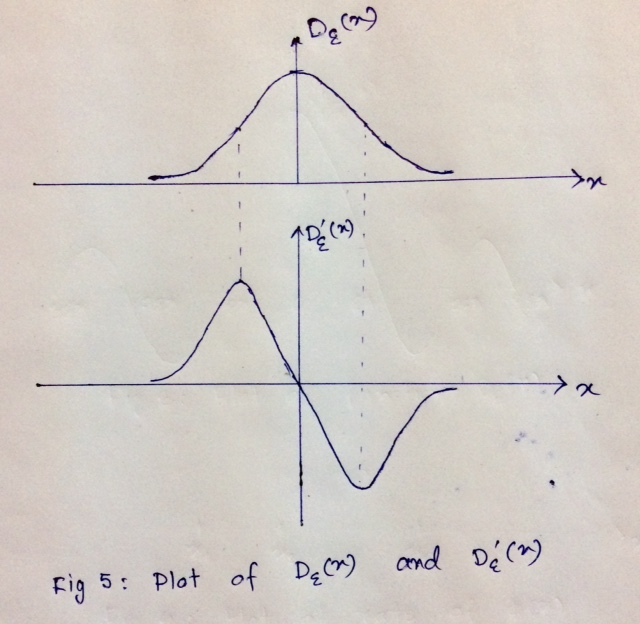
\includegraphics[width=0.8\textwidth]{DiracDeltaFig5.jpg}
\end{center}
As $\epsilon \to 0$, each of these peaks becomes very narrow and very tall, and two peaks each approach very close to the origin. Now, an integration by parts gives
\begin{equation}
\int_{-\infty}^{\infty} dx D_\epsilon^\prime (x) f(x) = [D_\epsilon (x) f(x)]_{-\infty}^{\infty} - \int_{-\infty}^{\infty} dx D_\epsilon (x) f^\prime (x)
\end{equation}
Because $D_\epsilon (x)$ tends to zero as $x \to \pm \infty$, the first term on the right hand side vanishes unless f(x) explodes violently at infinity. So by letting $\epsilon \to 0$, we arrive at the definition of $\delta^\prime (x)$: 
\begin{equation}
\int_{-\infty}^{\infty} \delta^\prime (x) f(x) dx = - \int_{-\infty}^{\infty} \delta (x) f^\prime(x) dx = - f^\prime (0)
\end{equation}
From this, we immediately get 
\begin{equation}
x\delta^\prime (x) = - \delta (x)
\end{equation}
Conversely, it can be shown that the general solution of the equation $$xu(x)=\delta(x)$$ can be written as $$u(x) = - \delta^\prime (x) + c \delta(x)$$ where the second term arises from the homogeneous equation $$x\delta(x)=0$$
From eqn(15) it also follows that
\begin{equation}
\delta^\prime(-x) = - \delta^\prime(x)
\end{equation}
The n-th order derivative of $\delta(x)$ can be defined in the same way. We find
\begin{equation}
\int_{-\infty}^{\infty} \delta^{(n)} (x) f(x) dx = (-1)^n f(0)
\end{equation}
We can prove following properties:

1.$$\delta^{(m)} (x) = (-1)^m \delta^{(m)} (-x)$$

2.$$x^{m+1} \delta^{(m)} (x) = 0$$

3.$$x \delta^{(m)} (x) = -m \delta^{(m-1)} (x)$$

\section*{Integration Of The Delta Function}
Comsider the indefinite integral
\begin{equation}
\theta_\epsilon (x) = \int_{-\infty}^{x} D_\epsilon (y) dy
\end{equation}
A graph of $\theta_\epsilon (x)$ vs x is shown below:
\vspace{0.2cm}
\begin{center}
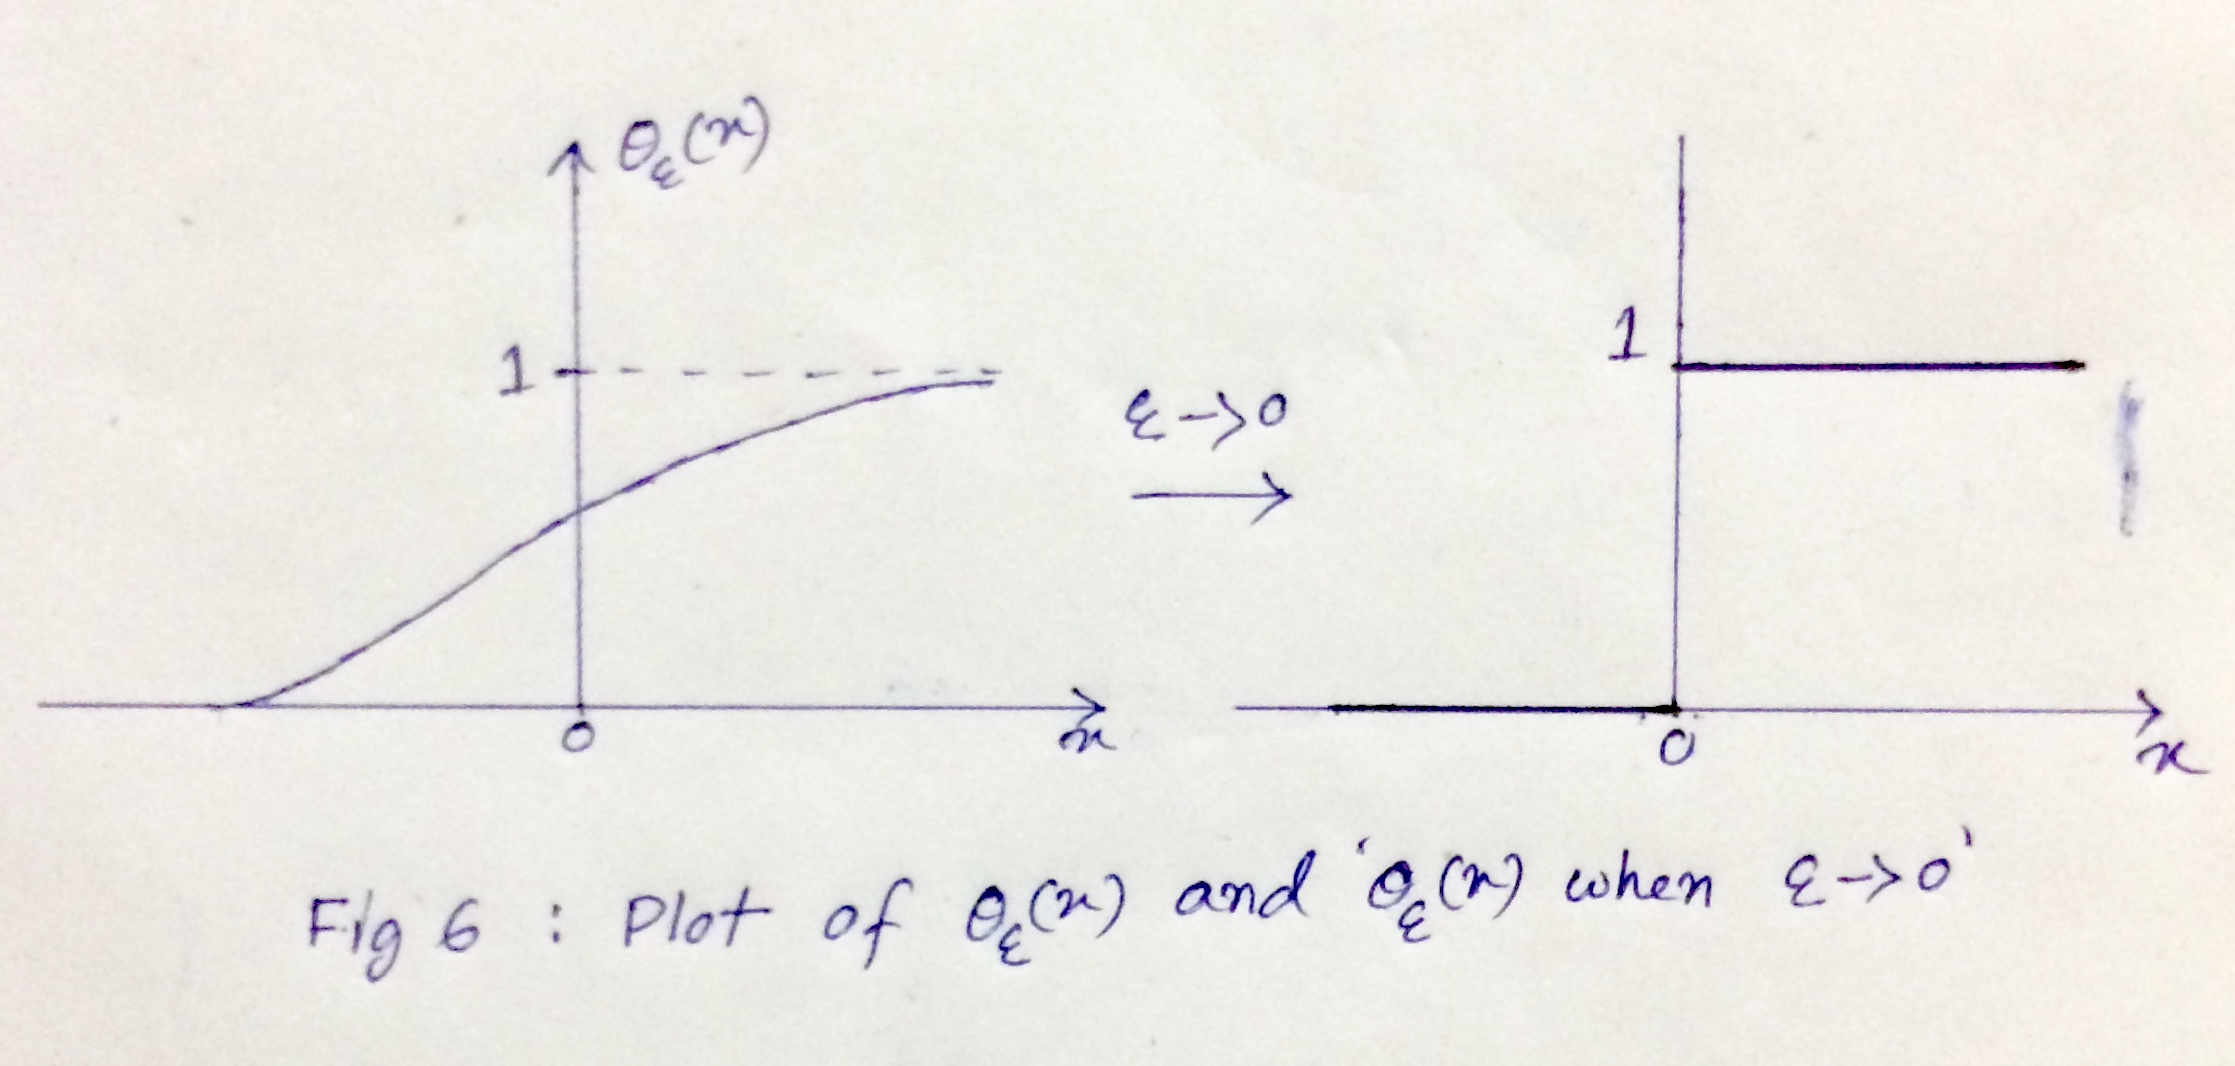
\includegraphics[width=0.8\textwidth]{DiracDeltaFig6.jpg}
\end{center}
As $\epsilon \to 0$, the step in the function $\theta_\epsilon (x)$ gets progressively steeper, until, finally, the function changes abruptly from 0 to 1 at x=0.
Thus, taking the limit $\epsilon \to 0$ in eqn(19), we have
\begin{equation}
\theta (x) = \int_{-\infty}^{x} \delta (x) dx
\end{equation}
where 
\begin{align*}
\theta (x) &= 1 \ \ \ for \ x>0\\
&=0 \ \ \ for \ x<0
\end{align*}
If we differentiate eqn(20) with respect to x, we get 
\begin{equation}
\frac{d\theta (x)}{dx} = \delta (x)
\end{equation}

\section*{Three Dimesional Delta Function}
We define $$\delta (\vec{r}) \equiv \delta (x) \delta (y) \delta (z)$$
In other words, $\delta (\vec{r})$ is zero if any of the coordinates x,y and z is not equal to zero and $\delta (\vec{r})$ tends to infinitely at the origin, i.e, when x=0, y=0 and z=0, such that $$\int_{volume} \delta (\vec{r}) d^3r = 1$$ if the volume of integration contains the origin. We also have $$\int_{volume} \delta (\vec{r}) f(\vec{r}) d^3r = f(0)$$ where again, the volume of integration contains the origin.

Note:

1. $$\delta (\vec{r} - \vec{r}^\prime) = \delta (x-x^\prime) \delta (y-y^\prime) \delta (z-z^\prime)$$

2.$$\delta (\vec{r} - \vec{r}^\prime) d^3r = 1$$ where the volume of integration includes the point $\vec{r}^\prime$, otherwise the integral is zero.

3.$$\int_{volume} \delta (\vec{r} - \vec{r}^\prime) f(\vec{r}) d^3r = f(\vec{r}^\prime)$$ if volume of integration includes the point $\vec{r}^\prime$

\section*{A Useful Formula}
Consider the integral 
\begin{align*}
\int_{-\infty}^{\infty} e^{ikx} dx &= \lim_{L \to \infty} \int_{-L}^{L} e^{ikx}dx \\
&= \lim_{L \to \infty} \frac{1}{ik} \left( e^{ikL} - e^{-ikL} \right) \\
&= \lim_{L \to \infty} \frac{2}{k} \left( \frac{e^{ikL} - e^{-ikL}}{2i} \right) \\
&= \lim_{L \to \infty} \frac{2}{k} \sin kL \\
&= 2\pi \lim_{L \to \infty} \frac{\sin kL}{\pi k} \\
&= 2\pi \delta (k) \\
\end{align*}
Since
\begin{align*}
& \lim_{\epsilon \to 0} \frac{\sin (x/\epsilon)}{\pi x} = \delta (x). \\
& Let, \ \epsilon = \frac{1}{L} \\
& So, \ when, \ L \to \infty, \ then \ \epsilon \to 0. \\
& therefore, \ \lim_{L \to \infty} \frac{\sin kL}{\pi k} = \lim_{\epsilon \to 0} \frac{\sin (k/\epsilon)}{\pi k} 
\end{align*}

Thus
\begin{equation}
\int_{-\infty}^{\infty} e^{ikx} dx = 2\pi \delta (k) 
\end{equation}

In eqn(22) if we integrated with respect to k, we would have $\delta (x)$ on the right handside
\begin{equation}
\int_{-\infty}^{\infty} e^{ikx} dk = 2\pi \delta (x) 
\end{equation}
Also note that in eqn(22) we are integrating over x over its full range of values. Making a change of variable $x \to -x$ does not change the value of the integral. Here we also have 
\begin{equation}
\int_{-\infty}^{\infty} e^{-ikx} dx = 2\pi \delta (k) 
\end{equation}
Similarly in eqn(23), making the change of variable $k \to -k$, doesn't change the value of the integral. So we could also with 
\begin{equation}
\int_{-\infty}^{\infty} e^{-ikx} dk = 2\pi \delta (x) 
\end{equation}
Thus in summery,
\begin{align*}
\int_{-\infty}^{\infty} e^{\pm ikx} dx = 2\pi \delta (k) 
\end{align*}
\begin{align*}
\int_{-\infty}^{\infty} e^{\pm ikx} dk = 2\pi \delta (x) 
\end{align*}
In three dimension
\begin{align*}
\int_{all \ space} e^{\pm i \vec{k}.\vec{r}} d^3r = (2\pi)^3 \delta (\vec{k}) 
\end{align*}
\begin{align*}
\int_{all \ space} e^{\pm i (\vec{k} - \vec{k}^\prime).\vec{r}} d^3r = (2\pi)^3 \delta (\vec{k} - \vec{k}^\prime) 
\end{align*}
\begin{align*}
\int_{all \ space} e^{\pm i \vec{k}.(\vec{r} - \vec{r}^\prime)} d^3k = (2\pi)^3 \delta (\vec{r} - \vec{r}^\prime) 
\end{align*}

\section*{Fourier Transform}
We can always express a function f(x) in the form 
\begin{equation}
f(x) = \int_{-\infty}^{\infty} e^{ikx} \tilde{f}(k) dk
\end{equation}
where $\tilde{f}(k)$ is a function of k, called the fourier transform of f(x). From eqn(26) we can write 
\begin{align*}
\int_{-\infty}^{\infty} e^{-ik^\prime x} f(x) dx &= \int_{-\infty}^{\infty} \int_{-\infty}^{\infty} e^{i(k-k^\prime) x} \tilde{f}(k) dk dx \\
&= (2\pi) \int_{-\infty}^{\infty} \delta(k - k^\prime) \tilde{f}(k) dk \\
&= (2\pi) \tilde{f}(k^\prime) 
\end{align*}
Thus,
\begin{equation}
\tilde{f}(k) = \frac{1}{2 \pi} \int_{-\infty}^{\infty} e^{-ikx} f(x) dx
\end{equation}
The function f(x) and $\tilde{f} (k)$ are Fourier transform of each other. We can write eqn(26) and eqn(27) in a more symmetrical fashion as follows
\begin{equation}
f(x)= \frac{1}{\sqrt{2 \pi}} \int_{-\infty}^{\infty} e^{ikx} \tilde{f}(k) dk
\end{equation}
\begin{equation}
\tilde{f}(k) = \frac{1}{\sqrt{2 \pi}} \int_{-\infty}^{\infty} e^{-ikx} f(x) dx
\end{equation}
In three dimension, we can write
\begin{equation}
f(\vec{r})= \frac{1}{(2 \pi)^{3/2}} \int_{all\ k \ space}  e^{i \vec{k}.\vec{r}} \tilde{f}(\vec{k}) d^3k
\end{equation}
Multiplying this equation by $e^{-i \vec{k}.\vec{r}}$ and integrating over $\vec{r}$, we have
\begin{align*}
\int_{all\ space}  e^{-i \vec{k}^\prime.\vec{r}} f(\vec{r}) d^3r &= \frac{1}{(2 \pi)^{3/2}} \int d^3r \int d^3k e^{i(\vec{k} - \vec{k}^\prime).\vec{r}} \tilde{f}(\vec{k}) \\
&= \frac{1}{(2 \pi)^{3/2}} \int d^3k (2 \pi)^3 \delta (\vec{k} - \vec{k}^\prime) \tilde{f}(\vec{k}) \\
&= (2 \pi)^{3/2} \tilde{f}(\vec{k}^\prime)
\end{align*}
Therefore,
\begin{align*}
\tilde{f}(\vec{k}) = \frac{1}{(2 \pi)^{3/2}} \int e^{-i \vec{k}.\vec{r}} f(\vec{r}) d^3r  
\end{align*}
Thus, if we write
\begin{align*}
f(\vec{r}) = \frac{1}{(2 \pi)^{3/2}} \int e^{i \vec{k}.\vec{r}} \tilde{f}(\vec{k}) d^3k 
\end{align*}
then
\begin{align*}
\tilde{f}(\vec{k}) = \frac{1}{(2 \pi)^{3/2}} \int e^{-i \vec{k}.\vec{r}} \tilde{f}(\vec{r}) d^3r 
\end{align*}

\section*{Parseval Identity}
We can now prove the important identity
\begin{align*}
\int |f(\vec{r})|^2 d^3r = \int |\tilde{f}(\vec{k})|^2 d^3k
\end{align*}
\underline{PROOF:}
\begin{align*}
\int |f(\vec{r})|^2 d^3r &= \int f(\vec{r}) f^*(\vec{r}) d^3r \\
&= \int d^3r \ .\ \frac{1}{(2\pi)^{3/2}} \int e^{i \vec{k}.\vec{r}} \tilde{f} (\vec{k}) d^3k \ .\ \frac{1}{(2\pi)^{3/2}} \int e^{-i \vec{k}^\prime.\vec{r}} \tilde{f}^* (\vec{k}^\prime) d^3k^\prime \\
&= \frac{1}{(2\pi)^3} \int d^3k d^3k^\prime \tilde{f} (\vec{k}) \tilde{f}^* (\vec{k}^\prime) \int d^3r e^{i (\vec{k} - \vec{k}^\prime) . \vec{r}} (2\pi)^3 \delta (\vec{k} - \vec{k}^\prime) \\
&= \int d^3k d^3k^\prime \tilde{f} (\vec{k}) \tilde{f}^* (\vec{k}^\prime) \delta (\vec{k} - \vec{k}^\prime) \\
&= \int d^3k \tilde{f} (\vec{k}) \tilde{f}^* (\vec{k}) \\
&= \int |\tilde{f} (\vec{k})|^2  d^3k  \\
\end{align*}





%
%	Consider the function $D_\epsilon(x)$ given by
%	\begin{eqnarray}
%	D_\epsilon(x) &= 
%		\begin{cases}
%			\frac{1}{\epsilon} \ \ &\text{for} \ \  -\frac{\epsilon}{2} \leq x \leq \frac{\epsilon}{2} \\
%			0 \ \ &\text{for} \ \  |x| > \frac{\epsilon}{2} 
%		\end{cases}
%	\end{eqnarray}
%	where $\epsilon$ is a positive parameter. The plot of the function is shown in figure (\ref{fig.cpt1.figure1}).
%	
%	\begin{figure}
%		\centering
%		\subfloat[]{\includegraphics[width=5cm]{delta.pdf}}
%		\caption{Dirac Delta Function}
%		\label{fig.cpt1.figure1}
%	\end{figure}
%	
%	The integral of the function with respect to $x$ is $1$, i.e.,
%	\begin{equation}
%		\int_{-\infty}^{\infty} D_\epsilon(x) dx = 1
%	\end{equation}
%	Now imagine making $\epsilon$ smaller. As we decrease $\epsilon$, the function gets narrower and taller, but the integral of the function(i.e., the area under graph remains constant at the value $1$).
%	In the limit $\epsilon \rightarrow 0$, the function $D_\epsilon(x)$ collapses to a single  point $x=0$ and gets infinitely tall. So $\lim\limits_{\epsilon \rightarrow \epsilon} D_\epsilon(x)$ is not a function at all and the procedure of taking the limit is not justified.
%	\\
%	
%	However, we can make the limiting procedure meaningful if multiply $D_\epsilon(x)$ by some well defined function $f(x)$, integrate over $x$ and then take the limit $\epsilon \rightarrow 0 $. consider the integral
%	\begin{equation}
%		\int_{-\infty}^{\infty} D_\epsilon(x) f(x) dx
%	\end{equation}
%	where $f(x)$ is a well-defined function. If $\epsilon$ is significantly small, the variation of $f(x)$ over the effective integration interval $[-\epsilon / 2, \epsilon / 2]$ is negligible and $f(x)$ remains practically equal to $f(0)$, therefore,
%	\begin{equation}
%		\int_{-\infty}^{\infty} D_\epsilon (x) f(x) dx \simeq f(0) \int_{-\infty}^{\infty} D_\epsilon (x) dx = f(0)
%	\end{equation}
%	The smaller the value of $\epsilon$, the better the approximation. In the limit $\epsilon \rightarrow 0$, the above equation is exact
%	\begin{equation}
%		\lim\limits_{\epsilon \rightarrow 0}\int_{-\infty}^{\infty} D_\epsilon (x) f(x) dx  = f(0)
%	\end{equation}
%	Now, we define the delta function by the relation
%	\begin{equation}
%		\int_{-\infty}^{\infty} \delta(x) f(x) dx \  _=^{def}  \lim\limits_{\epsilon \rightarrow 0}\int_{-\infty}^{\infty} D_\epsilon (x) f(x) dx  = f(0)
%	\end{equation}
%	This equation is valid for any function $f(x)$ defined at the origin. More generally, $\delta(x - x_0)$ is defined as,
%	\begin{equation}
%		\int_{-\infty}^{\infty} \delta(x - x_0) f(x) dx \ = f(x_0)
%	\end{equation}
%	Actually, the integral notation $\int_{-\infty}^{\infty} \delta(x) f(x) dx$ is not justified because $\delta(x)$ is not really a function. Physically, there is no problem since it becomes impossible to distinguish between $D_\epsilon(x)$ and $\delta(x)$ as soon as $\epsilon$ becomes negligible compared to all distances involved in a physical problem. Whenever a mathematical difficulty might arise, all we need to do is to assume that $\delta(x)$ is actually $D_\epsilon(x)$ with $\epsilon$ extremely small but not strictly zero.
%	\\
%	Formally, we can express $\delta(x)$ as a limit of a square of proper functions : 
%	\begin{equation}
%		\lim\limits_{\epsilon \rightarrow 0} D_\epsilon(x) \equiv \delta(x)
%	\end{equation}
%	Here $D_\epsilon(x)$, which is a proper function of $x$ is called the representation of the delta function. One representation is the "square function" given at the beginning. The representation is not unique. There are other functions which approach the delta function when appropriate limits are taken.
%	
%	\section{Other representation of delta function}
%		\begin{enumerate}
%			\item 
%			Consider the function
%			\begin{equation}
%				D_\epsilon(x) = \frac{1}{\epsilon \sqrt{\pi}} e^{-x^2/\epsilon^2}  \ \ \ (\epsilon > 0)
%				\label{eqn.other-reps-exp}
%			\end{equation}
%			For each value of the parameter $\epsilon$, this function satisfies
%			\begin{equation}
%			\int_{-\infty}^{\infty} D_\epsilon(x) dx = 1
%			\end{equation}
%		
%		\begin{figure}
%			\centering
%			\subfloat[]{\includegraphics[width=5cm]{chapter1-delta-reps-exp.pdf}}
%			\subfloat[]{\includegraphics[width=5cm]{chapter1-delta-reps-sine.pdf}}
%			\caption{Plot of function $D_\epsilon(x)$ for (a) equation (\ref{eqn.other-reps-exp}) (b) and equation (\ref{eqn.other-reps-sin})}
%			\label{fig.cpt1.figure2}
%		\end{figure}
%		
%		
%		When plotted against $x$, the function has a peak at the origin. The peak has a height of $\frac{1}{\epsilon \sqrt{\pi}}$ and a width of order $\epsilon$ (exactly how the width is defined doesn't matter). So if $\epsilon$ is allowed to become very small, the peak becomes very tall and very narrow. Outside the peak the function becomes extremely small. Thus we have
%		\begin{equation}
%		\delta(x) = \lim\limits_{\epsilon \rightarrow 0}\frac{1}{\epsilon \sqrt{\pi}} e^{-x^2/\epsilon^2}
%		\end{equation}
%		
%		%% proof
%		
%		\item
%		Consider another function
%		\begin{equation}
%			D_\epsilon(x) = \frac{1}{\pi} \frac{\sin(x/\epsilon)}{x} \ \ \ \ (\epsilon > 0)
%			\label{eqn.other-reps-sin}
%		\end{equation} 
%		
%
%		
%		For any value of the parameter $\epsilon$ we have 
%		\begin{equation}
%			\int_{-\infty}^{\infty} D_\epsilon(x) dx = 1
%		\end{equation}
%		A plot of the function $D_\epsilon(x)$ shows that it has the value $\frac{1}{\epsilon \pi}$ at $x=0$ and it oscillates with decreasing amplitude as $|x|$ increases. The width of the central maxima is of the order of $\epsilon$ and the period of oscillation with respect to $x$ is $2 \pi \epsilon$.\\
%		Thus the limit of this function as $\epsilon \rightarrow 0 $ has all the properties of the delta function : it becomes infinitely large at $x=0$, it has unit integral, and infinitely rapid oscillations as $|x|$ increases means that the entire contribution to an integral containing this function comes from an infinitesimal neighborhood of $x=0$.\\
%		We can therefore write,
%		\begin{equation}
%			\delta(x) = \lim\limits_{\epsilon \rightarrow 0} \frac{1}{\pi} \frac{\sin(x/\epsilon)}{x}
%		\end{equation}
%
%		\item
%		We can also show that
%		\begin{eqnarray}
%			\delta(x) &= \lim\limits_{\epsilon \rightarrow 0} \frac{1}{2\epsilon} e^{-|x| / \epsilon} \\
%			\delta(x) &= \lim\limits_{\epsilon \rightarrow 0} \frac{1}{\pi} \frac{\epsilon}{x^2 + \epsilon^2} \\
%			\delta(x) &= \lim\limits_{\epsilon \rightarrow 0} \frac{\epsilon}{\pi} \frac{\sin^2(x/\epsilon)}{x^2}
%		\end{eqnarray}
%		
%		\end{enumerate}	
%	\section{Properties of the delta function}
%		It is important to note that, because of its singular $@@@@@@$ , the $\delta$ function cannot be the end result of a calculation, and has meaning only so long as a subsequent integral over its argument is carried out. With this understanding we can write down some relations between delta functions.
%		\begin{enumerate}[label=\textbf{Property \ \arabic*},start=1]
%			\item 
%			The delta function is a even function
%			\begin{equation}
%				\delta(-x) = \delta(x)
%			\end{equation}
%			
%			\item
%			\begin{equation}
%				x \delta(x) = 0
%			\end{equation}
%			
%			\item
%			\begin{equation}
%			\delta(a x) = \frac{1}{|a|} \delta(x)
%			\end{equation}
%			proof: Consider the integral
%			\begin{equation}
%				I = \int_{-\infty}^{\infty} \delta(a x) f(x) dx
%			\end{equation}
%			Since the delta function is even in its argument, it doesn't matter if we replace $a$ by $|a|$ in the argument. Thus
%			\begin{equation}
%				I = \int_{-\infty}^{\infty} \delta(|a| x) f(x) dx
%			\end{equation}
%			Making the change in variable $ y = |a| x$ we have,
%			\begin{eqnarray}
%				I &= \frac{1}{|a|}\int_{-\infty}^{\infty} \delta(y) f(y/|a|) dx \nonumber \\
%				&= \frac{1}{|a|} f(0) \nonumber
%			\end{eqnarray}			
%			or
%			\begin{equation}
%				\int_{-\infty}^{\infty} \delta(a x) f(x) dx = \frac{1}{|a|} \int_{-\infty}^{\infty} \delta(x) f(x) dx
%			\end{equation}
%			or
%			\begin{equation}
%				\delta(a x) = \frac{1}{|a|} \delta(x)
%			\end{equation}
%			
%			
%			\item
%			More generally
%			\begin{equation}
%				\delta(\phi(x)) = \sum_{i} \frac{\delta(x - x_i)}{\left|\frac{\partial\phi}{\partial x}\right|_{x_i}}
%			\end{equation}
%			where the sum sums over the $x_i$'s which are simple roots of $\phi(x)$.
%			
%			proof : let $x_1 , x_2, \ldots , x_N$ be the simple roots of $\phi(x)$,
%			
%			%figure
%			
%			In the neighborhood of any one of the simple roots $x_i$, we can write
%			@@@@@@@
%			\begin{equation}
%				\phi(x) = (x - x_i) \psi(x)
%			\end{equation}
%			or ???????
%			\begin{equation}
%				\phi(x) = (x - x_i) \psi(x_i)
%			\end{equation}
%			
%			where $\psi(x_i) \neq 0$. We have
%			\begin{equation}
%				\psi(x_i) = \left|\frac{\partial \phi(x)}{\partial x} \right|_{x=x_i}
%			\end{equation}
%			Now, consider the integral
%			\begin{eqnarray}
%				I &= \int_{-\infty}^{\infty} \delta(\phi(x)) f(x) dx  \nonumber \\
%				&= \sum_{i=1}^{N} \int_{x_i - \epsilon}^{x_i + \epsilon} \delta[(x-x_i) \psi(x_i)] f(x) dx \nonumber \\
%				&= \sum_{i=1}^{N} \frac{1}{|\psi(x_i)|}\int_{x_i - \epsilon}^{x_i + \epsilon} \delta(x-x_i) f(x) dx \nonumber \\
%				&= \sum_{i=1}^{N} \frac{1}{ \left|\frac{\partial \phi(x)}{\partial x} \right|_{x=x_i}}\int_{-\infty}^{\infty} \delta(x-x_i) f(x) dx \nonumber \\
%				&= \sum_{i=1}^{N} \frac{1}{ \left|\frac{\partial \phi}{\partial x} \right|_{x=x_i}} f(x_i) \nonumber
%			\end{eqnarray}
%			The above result is obtained if we write
%			\begin{equation}
%				\delta(\phi(x)) = \sum_{i=1}^{N} \frac{\delta(x - x_i)}{\left|\frac{\partial \phi}{\partial x}\right|_{x=x_i}}
%			\end{equation}
%			
%			
%			\item
%			A frequently used example of the above result is
%			\begin{equation}
%				\delta(x^2 - a^2) = \frac{1}{2 a} \delta(x - a) + \frac{1}{2 a} \delta(x + a) \ \ \ \ (a > 0)
%			\end{equation}
%			
%			Here
%			\begin{equation}
%				\phi(x) = x^2 - a^2 = (x-a)(x+a)
%			\end{equation}
%				The two simple roots of $\phi(x)$ are at $x=a $ and $x=-a$. Now
%				\begin{eqnarray}
%					\left|\frac{\partial \phi}{\partial x}\right|_{x=a} = \left|2 x\right|_{x=a} = 2a  \\
%					\left|\frac{\partial \phi}{\partial x}\right|_{x=a} = \left|-2 x\right|_{x=-a} = 2a 
%				\end{eqnarray}
%				$\therefore$ The above result follows.
%				
%				\item
%				\begin{equation}
%					f(x) \delta(x-a) = f(a) \delta(x-a)
%				\end{equation}
%
%				\item
%				\begin{equation}
%					\int \delta(x-y) \delta(y-a) dy = \delta(x-a)
%				\end{equation}
%				
%			
%		\end{enumerate}
%		
%		\subsection{Notes}
%		\begin{enumerate}[label=\textbf{Note : \ \arabic*},start=1]
%			\item 
%			We have the identity
%			\begin{equation}
%				x\delta(x) = 0
%			\end{equation}
%			The converse is also true and it can be shown that the equation
%			\begin{equation}
%				x u(x) = 0
%			\end{equation}
%			has the general solution
%			\begin{equation}
%				u(x) = c \delta(x)
%			\end{equation}
%			
%			
%			\item
%			We will now prove an identity which is particularly useful in Quantum Mechanics.
%			\begin{equation}
%				\lim\limits_{\epsilon \rightarrow 0^+} \int_{-\infty}^{\infty} \frac{1}{x \pm \imath \epsilon} f(x) dx = \rho \int_{-\infty}^{\infty} \frac{dx}{x}f(x) \mp \imath\pi f(0)
%			\end{equation}
%			or in short
%			\begin{equation}
%				\lim\limits_{\epsilon \rightarrow 0^+} \frac{1}{x \pm \imath \epsilon} = \rho(\frac{1}{x}) \mp \imath \pi \delta(x)
%			\end{equation}
%			Where it is understood that the second of these two equations have meaning only within an integral.\\
%			The symbol $\rho$ means principle part of an integral where the integral has a single pole. The principle part is defined as
%			\begin{equation}
%				\rho \int_{-A}^{B} \frac{dx}{x} f(x) dx = \lim\limits_{\eta \rightarrow 0^+} \left[\int_{-A}^{-\eta} + \int_{\eta}^{B}\right] \frac{dx}{x} f(x)
%			\end{equation}
%			\textbf{proof :}
%			\begin{equation}
%				\frac{1}{x \pm \imath \epsilon} = \frac{x \mp \imath\epsilon}{x^2 + \epsilon^2} = \frac{x}{x^2 + \epsilon^2} \mp \frac{\imath \epsilon}{x^2 + \epsilon^2}
%			\end{equation}
%			Now we have
%			\begin{eqnarray}\label{eqn:1}
%				\lim\limits_{\epsilon \rightarrow 0^+} \frac{1}{\pi} \frac{\epsilon}{x^2 + \epsilon^2} &= \delta(x) \nonumber \\
%				\lim\limits_{\epsilon \rightarrow 0^+} (\mp) \imath \frac{\epsilon}{x^2 + \epsilon^2} &= \mp \imath \pi \delta(x)
%			\end{eqnarray}
%			Now consider the first term on the right hand side of equation  \ref{eqn:1}. We multiply this term by a function $f(x)$ which is regular at the origin and then integrate over $x$. We get
%			\begin{equation}\label{eqn:2}
%				\lim\limits_{\epsilon \rightarrow 0^+} \int_{-\infty}^{\infty} \frac{x f(x)}{x^2 + \epsilon^2} dx
%				=\lim\limits_{\epsilon \rightarrow 0^+}\left[
%				\lim\limits_{\eta \rightarrow 0^+}\left[ \int_{-\infty}^{-\eta} \frac{x f(x)}{x^2 + \epsilon^2}
%				+\int_{-\eta}^{\eta} \frac{x f(x)}{x^2 + \epsilon^2}
%				+\int_{\eta}^{\infty} \frac{x f(x)}{x^2 + \epsilon^2} dx\right]\right]
%			\end{equation}
%			Note that we take the limit over $\eta$ first and then we take the limit over $\epsilon$. Consider now the second integral above
%			\begin{equation} 
%				\lim\limits_{\eta \rightarrow 0^+} \int_{-\eta}^{+\eta} \frac{x f(x)}{x^2 + \epsilon^2} = f(0) \lim\limits_{\eta \rightarrow 0^+} \frac{1}{2}  \left[\ln({x^2 + \epsilon^2}
%				)\right]_{x=-\eta}^{x=\eta} = 0
%			\end{equation}
%			If we now reverse the order of the evaluation of limits in equation \ref{eqn:2}, the $\epsilon \rightarrow 0$ limit causes no difficulties in the other two integrals.
%			Thus we have
%			\begin{eqnarray}
%				&\lim\limits_{\epsilon \rightarrow 0^+} \int_{-\infty}^{\infty} \frac{x dx}{x^2 + \epsilon^2} f(x)\nonumber \\
%				 = &\lim\limits_{\eta \rightarrow 0^+} \lim\limits_{\epsilon \rightarrow 0^+} \left[\int_{-\infty}^{-\eta} + \int_{\eta}^{\infty}\right] \frac{x dx}{x^2 + \epsilon^2} f(x) \nonumber \\
%				 = &\lim\limits_{\eta \rightarrow 0^+} \left[\int_{-\infty}^{-\eta} + \int_{\eta}^{\infty}\right] \frac{dx}{x} f(x) \nonumber\\
%				 = & \rho \int_{-\infty}^{\infty} \frac{1}{x} f(x) dx \nonumber
%			\end{eqnarray}
%			This establishes the identity.
%		\end{enumerate}
%		
%	\section{Derivatives of the delta function}
%		One may define the derivative $\delta^\prime(x)$ of the delta function. When $\epsilon$ is small, the derivative of $D_\epsilon(x)$ has two peaks close to the origin, one peak is positive and the other is negative as drawn in the figure below
%		
%		\begin{figure}
%			\centering
%			\subfloat[]{\includegraphics[height=8cm,width=5cm]{chapter1-delta-reps-exp-derivative.pdf}}
%			\caption{(a) Derivative of Delta Function}
%			\label{}
%		\end{figure}
%		% figure
%		
%		
%		As $\epsilon \rightarrow 0$, each of these peaks becomes very narrow and very tall, and two peaks each approach very close to the origin. \\
%		Now the integration by parts gives
%		\begin{equation}
%			\int_{-\infty}^{\infty} dx D_\epsilon^\prime(x) f(x) = \left[D_\epsilon(x) f(x)\right]_{-\infty}^{\infty} - \int_{-\infty}^{\infty} dx D_\epsilon(x) f^\prime(x)
%		\end{equation}
%		Because $D_\epsilon(x)$ tens to zero as $x \rightarrow \pm \infty$, the first term on the right hand side vanishes unless $f(x)$ $@@@@@@@$ violently at infinity. So by letting $\epsilon \rightarrow 0$, we arrive at the definition of $\delta^\prime(x)$
%		\begin{equation}\label{eqn:3}
%			\int_{-\infty}^{\infty} \delta^\prime(x) f(x) dx = - \int_{-\infty}^{\infty} \delta(x) f^\prime(x) dx = - f^\prime(0)
%		\end{equation}
%		From this we immediately get
%		\begin{equation}
%			x \delta^\prime(x) = -\delta(x)
%		\end{equation}
%		Conversely, it can be shown that the general solution of the equation
%		\begin{equation}
%			x u(x) = \delta(x)
%		\end{equation}
%		can be written as
%		\begin{equation}
%			u(x) = -\delta^\prime(x) + c \delta(x)
%		\end{equation}
%		Where the second term arises from the homogeneous equation $x \delta(x) = 0$.
%		From equation  \ref{eqn:3}  it also follows that 
%		\begin{equation}
%			\delta^\prime(-x) = - \delta^\prime(x)
%		\end{equation}
%		The $n^{th}$ order derivative of $\delta(x)$ can be defined in the same way. We find
%		\begin{equation}
%			\int_{-\infty}^{\infty} \delta^{(n)}(x) f(x) dx = (-1)^{n} f(0)
%		\end{equation}
%		We can prove the following properties:
%		\begin{eqnarray}
%			\delta^{(m)}(x) &= (-1)^m \delta^{(m)} (-x) \\
%			x^{m+1} \delta^{(m)}(x) &= 0 \\
%			x\delta^{(m)}(x) &= -m \delta^{(m-1)} (x)
%		\end{eqnarray}
%		
%		
%	\section{Integration of the delta function}
%		Consider the indefinite integral
%		\begin{equation}\label{eqn:4}
%			\Theta_\epsilon(x) = \int_{-\infty}^{x}  D_\epsilon(y) dy
%		\end{equation}
%		A graph of $\Theta_\epsilon(x)$ vs $x$ is shown below
%		
%		%figure
%		
%		As $\epsilon \rightarrow 0$, the step in the function $\Theta_\epsilon(x)$ gets progressively steeper, until, finally, the function changes abruptly from $0$ to $1$ at $x=0$.
%		Thus taking the limit $\epsilon \rightarrow 0$ in equation \ref{eqn:4} we have
%		\begin{equation}\label{eqn:5}
%			\Theta(x) = \int_{-\infty}^{x} \delta(x) dx
%		\end{equation}
%		Where
%		\begin{equation}
%			\Theta(x) = 
%			\begin{cases}
%				1 \ \ \text{for} \ \ x > 0 \\
%				0 \ \ \text{for} \ \ x < 0
%			\end{cases}
%		\end{equation}
%		If we differentiate equation \ref{eqn:5} with respect to $x$,\\
%		we get
%		\begin{equation}
%			\frac{d \Theta(x)}{dx} = \delta(x)
%		\end{equation}
%		
%	\section{Three - dimensional delta function}
%		\begin{equation}
%			\delta(\vec{r}) _=^{def} \delta(x) \delta(y) \delta(z)
%		\end{equation}
%		In other words, $\delta(\vec{r})$ is zero if any of the coordinates $x, y, z$ is not equal to zero and $\delta(\vec{r})$ tends to infinity at the origin, i.e., when $x=0, y=0, z=0$, such that 
%		\begin{equation}
%			\int_{volume} \delta(\vec{r}) d^3 r = 1
%		\end{equation}
%		if the volume of the integration contains the origin. We also have
%		\begin{equation}
%			\int \delta(\vec{r}) f(\vec{r}) d^3 r = f(0)
%		\end{equation}
%		where again the volume of the integration includes the origin.
%		\textbf{Note:}
%		\begin{eqnarray}
%			\delta(\vec{r} - \vec{r^\prime}) &= \delta(x - x^\prime) \delta(y - y^\prime) \delta(z-z^\prime) \\
%			\int_{v}\delta(\vec{r} - \vec{r^\prime}) d^3r &= 1
%		\end{eqnarray}
%		where the volume of integration includes the point $\vec{r}^\prime$. Otherwise the integral is zero.
%		\begin{equation}
%			\int_{v}\delta(\vec{r} - \vec{r^\prime}) f(\vec{r}) d^3r = f(\vec{r^\prime})
%		\end{equation}
%		if V includes the point $\vec{r^\prime}$.
%		
%		\textbf{A useful formula}
%		Consider the integral
%		\begin{eqnarray}
%			\int_{-\infty}^{\infty} e^{\imath k x} dx 
%			&= \lim\limits_{L \rightarrow \infty} \int_{-L}^{L} e^{\imath k x} dx \nonumber \\
%			&= \lim\limits_{L \rightarrow \infty} \frac{1}{\imath k} \left(e^{\imath k L} - e^{-\imath k L}\right) \nonumber \\
%			&= \lim\limits_{L \rightarrow \infty} \frac{2}{k} \left(\frac{e^{\imath k L} - e^{-\imath k L}}{2\imath}\right) \nonumber \\
%			&= \lim\limits_{L \rightarrow \infty} \frac{2}{k} \sin(k L) \nonumber \\
%			&= 2\pi \lim\limits_{L \rightarrow \infty} \frac{\sin(k L
%				)}{\pi k} \nonumber \\
%			&= 2\pi \delta(k)
%		\end{eqnarray}
%		using 
%		\begin{equation}
%			\lim\limits_{\epsilon \rightarrow 0} \frac{\sin(x /\epsilon
%				)}{\pi x} = \delta(x)
%		\end{equation}
%		Thus
%		\begin{equation}\label{eqn:6}
%			\int_{-\infty}^{\infty} e^{\imath k x} dx = 2\pi \delta(k)
%		\end{equation}
%		In equation \ref{eqn:6} if we integrate with respect to $k$, we would have $delta(x)$ on the right hand side,
%	
%	%%%%%%%%%%%%%%%%%%%%%%%%%%%% equation number
%	
%		\begin{equation}\label{eqn:100}
%		\int_{-\infty}^{\infty} e^{\imath k x} dk = 2\pi \delta(x)
%		\end{equation}
%		Also note that in equation \ref{eqn:6} we are integrating over its full range of values. Making a change of variable $x \rightarrow -x$ does not change the value of the integral. Hence we also have
%		
%		\begin{equation}\label{eqn:101}
%		\int_{-\infty}^{\infty} e^{-\imath k x} dx = 2\pi \delta(k)
%		\end{equation}
%		Similarly, in equation \ref{eqn:100} making the change $k \rightarrow -k$, doesn't change the value of the integral. So we could also write
%		\begin{equation}\label{eqn:102}
%		\int_{-\infty}^{\infty} e^{-\imath k x} dk = 2\pi \delta(x)
%		\end{equation}
%		
%		Thus in summary
%		\begin{eqnarray}\label{eqn:103-104}
%			\int_{\pm \infty}^{\infty} e^{-\imath k x} dx &= 2\pi \delta(k)
%			\int_{\pm \infty}^{\infty} e^{-\imath k x} dk &= 2\pi \delta(x)
%		\end{eqnarray}
%		In three dimensions
%		\begin{eqnarray}\label{eqn:105-107}
%			\int_{all\ space} e^{\pm \imath \vec{k} . \vec{r}} d^3\vec{r} &= (2\pi)^3 \delta(\vec{k}) \\
%			\int_{all\ space} e^{\pm \imath (\vec{k} - \vec{k^\prime}) . \vec{r}} d^3\vec{r} &= (2\pi)^3 \delta(\vec{k} - \vec{k^\prime}) \\
%			\int_{all\ space} e^{\pm \imath \vec{k} . (\vec{r} - \vec{r^\prime})} d^3\vec{r} &= (2\pi)^3 \delta(\vec{r} - \vec{r^\prime}) \\
%		\end{eqnarray}
%		
%	\section{Fourier Transformation}
%		We can always express a function $f(x)$ in the form
%		\begin{eqnarray}\label{eqn:108}
%			f(x) = \int_{-\infty}^{\infty} e^{\imath k x} \tilde{f}(k) dk
%		\end{eqnarray}
%		where $\tilde{f}(k)$ is a function of $k$, called the fourier transform of $f(x)$. From eqnarray \ref{eqn:108} we can write
%		
%		\begin{eqnarray}\label{eqn:109}
%			\int_{-\infty}^{\infty} e^{-\imath k^\prime x} f(x) dx 
%			&= \int_{-\infty}^{\infty} \int_{-\infty}^{\infty} e^{i(k-k^\prime) x} \tilde{f}(k) dk dk^\prime \nonumber \\
%			&= 2 \pi \int_{-\infty}^{\infty} \delta(k-k^\prime) \tilde{f}(k) dk \nonumber \\
%			&= 2\pi \tilde{f}(k^\prime) 
%		\end{eqnarray}
%		
%		Thus
%		\begin{eqnarray}\label{eqn:110}
%			\tilde{f}(k) = \frac{1}{2\pi} \int_{-\infty}^{\infty} e^{-\imath k x} f(x) dx
%		\end{eqnarray}
%		Thus functions $f(x)$ and $\tilde{f}(k)$ are Fourier transform of each other. We can write eqnarray \ref{eqn:108} and \ref{eqn:110} in a more symmetrical fashion as follows:
%		\begin{eqnarray}\label{eqn:111}
%		f(x) = \frac{1}{\sqrt{2\pi}} \int_{-\infty}^{\infty} e^{\imath k x} \tilde{f}(k) dk
%		\end{eqnarray}
%		\begin{eqnarray}\label{eqn:112}
%			\tilde{f}(k) = \frac{1}{\sqrt{2\pi}} \int_{-\infty}^{\infty} e^{-\imath k x} f(x) dx
%		\end{eqnarray}
%		In three dimension, we can write
%		\begin{eqnarray}\label{eqn:113}
%			f(\vec{r}) = \frac{1}{(2\pi)^{3/2}} \int_{all\ k-space} e^{i \vec{k} . \vec{r}} \tilde{f}(\vec{k}) d^3k
%		\end{eqnarray}
%		multiplying eqnarray \ref{eqn:113} by $e^{-i\vec{k^\prime} . \vec{r}} $ and integrating over $\vec{r}$, we have
%		\begin{eqnarray}\label{eqn:114}
%			\int_{all\ space} e^{-i\vec{k^\prime} . \vec{r}} f(\vec{r}) d^3 r
%			&= \frac{1}{(2\pi)^{3/2}} \int d^3 r \int d^3 k \ e^{i (\vec{k} - \vec{k^\prime}). \vec{r}} \tilde{f}(\vec{k}) \nonumber \\
%			&= \frac{1}{(2\pi)^{3/2}} \int d^3 k (2\pi)^3 \delta(\vec{k} - \vec{k^\prime}) \tilde{f}(\vec{k}) \nonumber \\
%			&= \frac{1}{(2\pi)^{-3/2}} \tilde{f}(\vec{k^\prime})
%		\end{eqnarray}
%		
%		Therefore
%		\begin{eqnarray}\label{eqn:115}
%			\tilde{f}(\vec{k}) = \frac{1}{(2\pi)^{3/2}} \int e^{-i\vec{k} . \vec{r}} f(\vec{r}) d^3 r
%		\end{eqnarray}
%		Thus we can write 
%		\begin{eqnarray}\label{eqn:116}
%		f(\vec{r}) = \frac{1}{(2\pi)^{3/2}} \int e^{i\vec{k} . \vec{r}} \tilde{f}(\vec{k}) d^3 k
%		\end{eqnarray}
%		\begin{eqnarray}\label{eqn:117}
%		\tilde{f}(\vec{k}) = \frac{1}{(2\pi)^{3/2}} \int e^{-i\vec{k} . \vec{r}} f(\vec{r}) d^3 r
%		\end{eqnarray}
%		
%		\textbf{Parseval's Identity:}\\
%		We can now  prove the important identity
%		\begin{eqnarray}\label{eqn:118}
%			\int |f(\vec{r})|^2 d^3r = \int |\tilde{f}(\vec{k})|^2 d^3k
%		\end{eqnarray}
%		proof:
%		\begin{eqnarray}
%			\int |f(\vec{r})|^2 d^3r
%			&= \int f(\vec{r}) f^*(\vec{r}) d^3r \nonumber \\
%			&= \int d^3r \frac{1}{(2\pi)^{3/2}} \int e^{\imath\vec{k} . \vec{r}} \tilde{f}(\vec{k}) d^3k \frac{1}{(2\pi)^{3/2}} \int e^{-\imath\vec{k^\prime} . \vec{r}} \tilde{f}^*(\vec{k^\prime}) d^3k^\prime \nonumber \\
%			&= \frac{1}{(2\pi)^3} \int d^3k\ d^3k^\prime \tilde{f}(\vec{k}) \tilde{f}^*(\vec{k^\prime}) \int d^3r \ e^{\imath(\vec{k} - \vec{k^\prime}).\vec{r}} \nonumber \\
%			&= \frac{1}{(2\pi)^3} \int d^3k\ d^3k^\prime \tilde{f}(\vec{k}) \tilde{f}^*(\vec{k^\prime}) (2\pi)^3 \delta(\vec{k} - \vec{k^\prime}) \nonumber \\
%			&= \int d^3k\ \tilde{f}(\vec{k}) \tilde{f}^*(\vec{k}) \nonumber \\
%			&= \int |\tilde{f}(\vec{k})|^2 d^3k
%		\end{eqnarray}
%		
%		
%		
%		
%		

\chapter{sheet-2 : Linear Vector Space}
%%% defining graphics path
\ifpdf
\graphicspath{{Chapter2/figs/}}
\else
\graphicspath{{Chapter2/figs/}}
\fi


%\chapter{sheet-2 : Linear Vector Space}
References
\begin{enumerate}
	\item 
	Quantum Mechanics	-	Shanker
	
	\item
	Quantum Mechanics	- Sakurai
\end{enumerate}

\section{Definition}
A linear vector space $V$ is a collection of objects $\psi_a, \psi_b, \ldots$, called vectors, which satisfy the following postulates:
\begin{enumerate}
	\item 
	If $\psi_a$ and $\psi_b$ are vectors in $V$, there is a unique vector $\psi_a + \psi_b$ in $V$, called the sum of $\psi_a $ and $\psi_b$. In other words, and operation called addition is defined in the vector space such that the space is closed under addition.
	
	\item 
	The vector addition is commutative and associative, i.e.,
	\begin{eqnarray}\label{eqn:2.1-2.2}
		\psi_a + \psi_b &= \psi_b + \psi_a \\
		\psi_a + (\psi_b + \psi_c) &= (\psi_a + \psi_b) + \psi_c
	\end{eqnarray}
	
	\item 
	There is a vector in $V$ called the null vector and denoted by $\phi$ satisfying
	\begin{equation}\label{eqn:2.3}
	\psi_a + \phi = \phi + \psi_a
	\end{equation}
	for every $\psi_a$ in $V$.
	
	\item 
	For every vector $\psi_a$ in $V$ there is another vector $\psi_a^\prime$ in $V$ such that
	\begin{equation}\label{eqn:2.4}
	\psi_a + \psi_a^\prime = \phi
	\end{equation}
	we denote $\psi_a^\prime$ as $-\psi_a$.\\
	(Note : we use the notation $\psi_a - \psi_b$ to mean $\psi_a + (-\psi_b$).
	
	\item 
	If $\psi_a$ is a vector and $\lambda$ is an arbitrary number (real or complex), called a scaler, there is a uniquely defined vector $\lambda \psi_a$ in $V$ satisfying.
	\begin{enumerate}
		\item 
		\begin{equation}\label{eqn:2.5}
		\lambda (\psi_a  + \psi_b) = \lambda \psi_a + \lambda + \psi_b
		\end{equation}
		i.e., multiplication is distributive with respect to vector addition.
		
		\item 
		\begin{equation}\label{eqn:2.6}
		(\lambda \mu) \psi_a = \lambda (\mu \psi_a)
		\end{equation}
		i.e., multiplication  by a scalar is associative.
		
		\item 
		\begin{equation}\label{eqn:2.7}
		(\lambda + \mu) \psi_a = \lambda \psi_a + \mu \psi_b
		\end{equation}
		i.e., multiplication is distributive with respect to addition scalars.
		
		\item 
		Multiplication by scalars $0$ and $1$ are defined by
		\begin{eqnarray}\label{eqn:2.8-2.9}
			0 \psi_a = \phi \\
			1 \psi_a = \psi_a
		\end{eqnarray}
		for any $\psi_a$ in $V$.
	\end{enumerate}
\end{enumerate}
\section{Example of linear vector space}
\begin{enumerate}
	\item 
	Consider all real numbers $x$ in the range $-\infty$ to $\infty$, i.e.,
	\begin{eqnarray}\label{eqn:2.10-2.11}
		-\infty < x < \infty \\
		x \in \Re \ \ \text{ ($\Re$ is the set of all real numbers )}
	\end{eqnarray}
	Take any two real numbers $x_1$ and $x_2$. If we add two real numbers we get another real number in $\Re$. Thus
	\begin{equation}\label{eqn:2.12}
	x_1 + x_2 = \Re
	\end{equation}
	Next take any real number $x$. If we multiply $x$ by another real number $\lambda$, we get a real number in $\Re$, i.e.,
	\begin{equation}\label{eqn:2.13}
	\lambda x \in \Re
	\end{equation}
	If we take a real number $x$, then there exists another real number $-x$ such that
	\begin{equation}\label{eqn:2.14}
	x + (-x) = 0
	\end{equation}
	So the real numbers form a vector space with the real numbers themselves as vectors in the space. The number $0$ is the null vector $\phi$ of the  space. The scalars $\lambda$ by which the vectors are multiplied are also real numbers.\\
	Thus the real numbers form a real linear vector space over a field which are also real numbers. The addition and multiplication are just the normal addition and multiplication of the real numbers.
	
	\item 
	The set of $n-tuples$ of numbers $(x_1, x_2, \ldots, x_n)$.
	When the addition of vectors and multiplication by a scalar are defined by
	\begin{equation}\label{eqn:2.15}
	(x_1 , x_2, \ldots, x_n) + (y_1 , y_2, \ldots, y_n) = (x_1 + y_1, x_2 + y_2, \ldots, x_n + y_n)
	\end{equation}
	and 
	\begin{equation}\label{eqn:2.16}
	\lambda (x_1, x_2, \ldots, x_n) = (\lambda x_1, \lambda x_2, \ldots, \lambda x_n)
	\end{equation}
	
	
	\item 
	The collection of all square-integrable complex valued functions of a real variable form a vector space. consider all functions
	\begin{equation}\label{eqn:2.17}
	f:\Re \rightarrow \mathbb{C}
	\end{equation}
	here, 
	$\Re $ =  set of real numbers \\
	$\mathbb{C}$  = set of complex numbers\\
	such that
	\begin{equation}\label{eqn:2.18}
	\int_{-\infty}^{\infty} f^*(x) f(x) dx \equiv \int_{-\infty}^{\infty} |f(x)|^2 dx < \infty \text{\  \ (i.e., finite)}
	\end{equation}
	The sum of two functions and the product of a function by a complex scalar are defined in the usual way.\\
	The reason the square-integrable functions form a (complex) vector space is that the space is closed under addition. The vectors of the space are the square-integrable functions. In other words, it can be shown that if $f$ and $g$ are two vectors, in this case two functions $f(x)$ and $g(x)$ both of which are square integrable, then $f(x) + g(x)$ is also square integrable and have the sum belong to the vector space.\\
	\textbf{proof:} \\
	Let $f(x)$ and $g(x)$ be two square integrable function, i.e., 
	\begin{equation}\label{eqn:2.19}
	\int_{-\infty}^{\infty} |f(x)|^2 dx < \infty
	\end{equation}
	and
	\begin{equation}\label{eqn:2.20}
	\int_{-\infty}^{\infty} |g(x)|^2 dx < \infty
	\end{equation}
	then using the inequality
	\begin{equation}\label{eqn:2.21}
	\int_{-\infty}^{\infty} |f+g|^2 dx \leq \left[\sqrt{\int_{\infty}^{\infty} |f|^2 dx} \sqrt{\int_{\infty}^{\infty} |g|^2 dx}\right]^2
	\end{equation}
	it is obvious that
	\begin{equation}\label{eqn:2.22}
	\int_{-\infty}^{\infty} |f+g|^2 dx < \infty
	\end{equation}
	(i.e., finite).
	
	\item 
	The set of all $n\times n$ matrices with complex elements form a complex linear vector space. For illustation let us take $2\times 2$ matrix $A$
	\begin{equation}\label{eqn:2.23}
	A = \left(			
	\begin{matrix}
	a & b \\
	c & d
	\end{matrix}
	\right)
	\end{equation}
	where the elements $a, b, c$ and $d$ can, in general, be complex. Then $A$ belongs to a vector (complex) space.
	We have
	
	\begin{eqnarray}\label{eqn:2.24-2.27}
		\phi &= \left(
		\begin{matrix}
			0 & 0 \\ 0 & 0
		\end{matrix}
		\right)\\
		\mathbb{I} &= \left(
		\begin{matrix}
			1 & 0 \\ 0 & 1
		\end{matrix}
		\right)\\
		-A &= \left(
		\begin{matrix}
			-a & -b \\ -c & -d
		\end{matrix}
		\right)\\
		\lambda A &= \left(
		\begin{matrix}
			\lambda a & \lambda b \\ \lambda c & \lambda d
		\end{matrix}
		\right)
	\end{eqnarray}
	The set of all these matrices form a vector space.						
\end{enumerate}

\section{Inner product space or a unitary vector space}\label{inner_product}
For a general linear vector space, product of vectors (i.e. multiplication of two vectors) need ot be defined. However, we will restrict ourselves to spaces in which a  scalar product or an inner product is defined.\\
A linear vector space is called unitary if a scalar product is defined in it. To every pair of vectors $\psi_a$ and $\psi_b$ in $V$ there corresponds a unique scalar (in general complex), called the scalar product. The scalar product is defined to have the following properties :
\begin{eqnarray}\label{eqn:2.28-2.32}
	(\psi_a , \psi_b) &= (\psi_b, \psi_a)^* \\
	(\psi_a , \lambda \psi_b) &= \lambda (\psi_a , \psi_b) \\
	(\lambda \psi_a , \psi_b) &= \lambda^* (\psi_a , \psi_b) \\
	(\psi_a , \psi_b + \psi_c) &= (\psi_a , \psi_b) + (\psi_a , \psi_c) \\
	(psi_a, \psi_a) \geq 0 \ \text{;the equality holds only if $\psi_a$ is the null vector}
\end{eqnarray}
It follows from the above postulated properties of the scalar product, that the scalar product is linear with respect to post factors, i.e.,
\begin{equation}\label{eqn:2.33}
(\psi_a, \lambda \psi_b + \mu \psi_c) = \lambda (\psi_a , \psi_b) + \mu (\psi_a , \psi_c)
\end{equation}
and anti-linear with respect to the pre factors, i.e.,
\begin{equation}\label{eqn:2.34}
(\lambda \psi_a + \mu \psi_b, \psi_c ) = \lambda^* (\psi_a , \psi_c) + \mu^* (\psi_b , \psi_c)
\end{equation}

\section{Examples of scalar product}
\begin{enumerate}[label=\textbf{Example \arabic*},start=1]
	\item 
	Consider the vector space consisting of all square integrable functions of a real variable in the domain $[a,b]$. This space is denoted by $L^2[a,b]$.\\
	Suppose
	\begin{equation}\label{eqn:2.35}
	f \in L^2[a,b]
	\end{equation}
	i.e.,
	\begin{equation}\label{eqn:2.36}
	\int_{a}^{b} f^*(x)f(x) dx \equiv \int_{a}^{b} |f(x)|^2 dx < \infty
	\end{equation}
	We can define the scalar product of two vectors $f$ and $g$ as
	\begin{equation}\label{eqn:2.37}
	(f, g) _\equiv^{def} \int_{a}^{b} f^*(x) g(x) dx = complex \ number
	\end{equation}
	We can show
	\begin{equation}\label{eqn:2.38}
	\left|(f, g)\right| = \left[\sqrt{\int_{a}^{b} |f(x)|^2 dx}\right] \left[\sqrt{\int_{a}^{b} |g(x)|^2 dx}\right]
	\end{equation}
	Since both $f$ and $g$ are square integrable, $|(f, g)|$ is finite, i.e., the scalar product of $f$ and $g$ exists.\\
	The scalar product defined above satisfies all the properties that a scalar product is postulated to have.
	
	
	\item 
	Now consider the vector space consisting of $n-tuples$ of complex numbers. Such a vector space is denoted as $\mathbb{C}^n$.\\
	A vector $\psi_a \in \mathbb{C}^n$ may be expressed as
	\begin{equation}\label{eqn:2.39}
	\psi_a = \left(
	\begin{matrix}
	a_1 & a_2 & \ldots & a_n
	\end{matrix}
	\right)^T
	\end{equation}
	The scalar product may then be defined as
	\begin{eqnarray}\label{eqn:2.40-2.41}
		(\psi_a , \psi_b) &_\equiv^{def} \left(
		\begin{matrix}
			a_1^* & a_2^* & \ldots &  a_3^*
		\end{matrix}
		\right)\left(
		\begin{matrix}
			b_1 \\ b_1 \\ \vdots \\ b_n
		\end{matrix}
		\right)\\
		&= \sum_{i=1}^{n} a_i^* b_i
	\end{eqnarray}
	This scalar product also satisfies all the properties of a scalar product.
	
	
	\item 
	Euclidean 3-space $\mathbb{R}^3$. The vectors of $\mathbb{R}^3$ are $3-tuples$ of real numbers which could be represented as column vectors . Thus if $psi_a$ and $\psi_b$ are in $\mathbb{R}^3$,
	\begin{eqnarray}\label{eqn:2.42-2.43}
		\psi_a &= \left(
		\begin{matrix}
			a1 \\ a2 \\ a3
		\end{matrix}
		\right)\\
		\psi_b &= \left(
		\begin{matrix}
			b1 \\b2 \\b3
		\end{matrix}
		\right)
	\end{eqnarray}
	where $a_i$ and $b_i$ are real. \\
	We could define the scalar product of $\psi_a$ and $\psi_b$ as
	\begin{eqnarray}\label{eqn:2.44-2.46}
		(\psi_a, \psi_b) &_\equiv^{def} 
		\left(
		\begin{matrix}
			a_1 & a_2 & a_3
		\end{matrix}
		\right)\left(
		\begin{matrix}
			b_1 \\ b_2 \\ b_3
		\end{matrix}
		\right) \\
		&= \psi_a^T \psi_b \\
		&- \sum_{i=1}^{3} a_i b_i
	\end{eqnarray}
	This scalar product also has all the postulated properties of a scalar product.\\
	
	In case of the vector space $\mathbb{R}^3$, the vectors $\psi_a$ and $\psi_b$ could be represented as directed lines $\vec{a}$ and $\vec{b}$ in a three dimensional coordinate system.\\
	
	\textbf{figure}
	\\
	The Scalar product $(\psi_a, \psi_b)$ is the usual dot product
	\begin{eqnarray}\label{eqn:2.47-2.48}
		\vec{a} . \vec{b} &= a_1 b_1 + a_2 b_2 + a_3 b_3 \\
		&= |\vec{a}||\vec{b}| \cos(\theta)
	\end{eqnarray}
	Where $|\vec{a}|$ and $|\vec{b}|$ are the magnitudes of the vectors $\vec{a}$ and $\vec{b}$ defined as
	\begin{eqnarray}\label{eqn:2.49-2.50}
		|\vec{a}| &\equiv \sqrt{(\psi_a , \psi_a)} = \sqrt{a_1^2 + a_2^2 + a_3^2} \\
		|\vec{b}| &\equiv \sqrt{(\psi_b, \psi_b)} = \sqrt{b_1^2 + b_2^2 + b_3^2}
	\end{eqnarray}
	
\end{enumerate}
\section{Norm of a vector}
If a vector space is enclosed with a scalar product, then the scalar product gives us the concept of the "magnitude" or "length" of a vector. In a general vector space the "magnitude" or "length" of a vector is called the norm of the vector. We simply define the norm of a vector $\psi_a$ as
\begin{equation}\label{eqn:2.51}
||\psi_a|| _\equiv^{def} \sqrt{(\psi_a, \psi_a)}
\end{equation}
The norm has the following properties:
\begin{enumerate}
	\item 
	\begin{equation}\label{eqn:2.52}
	||\psi_a|| \geq 0
	\end{equation}
	the equality holds only if the vector is null.
	
	\item 
	\begin{equation}\label{eqn:2.53}
	||\psi_a + \psi_b|| \leq ||\psi_a|| + ||\psi_b||
	\end{equation}
	This is called the triangle inequality
	
	\item 
	\begin{equation}\label{eqn:2.54}
	||\psi_a - \psi_b|| = ||\psi_b - \psi_a||
	\end{equation}
\end{enumerate}

\section{Metric included by the scalar product}
The norm included by the scalar product allows us to develop the concept of "distance" between vectors in a vector space. We say two vectors $\psi_a$ and $\psi_b$ are 'close' if $||\psi_a - \psi_b||$ is small. The metric in a vector space assigns a real number to the vector $\psi_a - \psi_b$. This real number is a measure of how close the two vectors are. We simply define the metric $\mathbf{d}(\psi_a, \psi_b)$ as
\begin{equation}\label{eqn:2.55}
\mathbf{d}(\psi_a, \psi_b) _\equiv^{def} ||\psi_a - \psi_b||
\end{equation}
Thus, if there are three vectors $\psi_a$, $\psi_b$ and $\psi_c$ and if $\mathbf{d}(\psi_a, \psi_b) < \mathbf{d}(\psi_a, \psi_c)$ then we say $\psi_a$ is closer to $\psi_b$ than to $\psi_c$.

\section{Schwarz's inequality}
We will now prove a very important inequality called Schwarz inequality which states
\begin{equation}\label{eqn:2.56}
|(\psi_a, \psi_b)| \leq \sqrt{(\psi_a, \psi_a)(\psi_b, \psi_b)}
\end{equation}
or
\begin{equation}\label{eqn:2.57}
|(\psi_a, \psi_b)| \leq ||\psi_a ||\ ||\psi_b||
\end{equation}
\textbf{proof : }
Let
\begin{equation}\label{eqn:2.58}
\psi = \psi_a + \lambda \psi_b
\end{equation}
Then
\begin{eqnarray}\label{eqn:2.59-2.60}
	(\psi, \psi) &= (\psi_a + \lambda \psi_b, \psi_a + \lambda \psi_b) \\
	&= (\psi_a, \psi_a) + \lambda (\psi_a, \psi_b) + \lambda^* (\psi_b, \psi_a) + |\lambda|^2 (\psi_b, \psi_b) \geq 0
\end{eqnarray}
The best inequality is obtained if $\lambda$ is chosen so as to minimize the left hand side of the above equation. By differentiation, the value of $\lambda$ which accomplishes this is found to be
\begin{equation}\label{eqn:2.61}
\lambda = - \frac{(\psi_b, \psi_a)}{\psi_b, \psi_b}
\end{equation}
Substituting this value of $\lambda$ in the above equation yields the Schwarz inequality.\\

We note that the equality sign holds if and only if $(\psi, \psi) = 0$, i.e., $\psi$ is the null vector, i.e., $\psi = \phi$, in other words
\begin{equation}\label{eqn:2.62}
\psi_a + \lambda \psi_b = \phi (null)
\end{equation}
i.e.,
\begin{eqnarray}\label{eqn:2.63-2.64}
	\psi_a &= - \lambda \psi_b + \phi \\
	\psi_a &= -\lambda \psi_b
\end{eqnarray}
Hence, the equality holds if $\psi_a$ and $\psi_b$ are multiple of each other, or if $\psi_a$ and $\psi_b$ are "parallel".\\
It follows from the Schwarz inequality that the scalar product $(\psi_a, \psi_b)$ is finite if the norms of $\psi_a$ and $\psi_b$ are finite.

\section{Analogy of Schwarz inequlity with vectors in a three-dimensional Euclidean space $\mathbb{R}^3$}
In $\mathbb{R}^3$, the vectors can be represented by directed lines (i.e. arrows). We have the scalar product ordinary vectors in the form
\begin{equation}\label{eqn:2.65}
\vec{A} . \vec{B} = |\vec{A}| \ |\vec{B}| \cos(\theta)
\end{equation}
Since cosine of any angle lies between $-1$ and $+1$, we have
\begin{equation}\label{eqn:2.66}
|\vec{A} . \vec{B} | \leq |\vec{A}| \ |\vec{B}|
\end{equation}
The analogue of this equation for a general vector space is the Schwarz inequality
\begin{equation}\label{eqn:2.67}
|(\psi_a, \psi_b)| \leq ||\psi_a|| \ ||\psi_b||
\end{equation}


\section{Orthogonality and linear independence}
A vector whose norm is unity is called a unit vector. For any given non-null vector, a unit vector can be formed by defining the vector by its norm. Thus
\begin{equation}\label{eqn:2.68}
u_a = \frac{\psi_a}{||\psi_a||}
\end{equation}
is normalized.\\
Two vectors $\psi_a$ and $\psi_b$ are orthogonal if their inverse product is zero, i.e., if
\begin{equation}\label{eqn:2.69}
(\psi_a, \psi_b ) = 0
\end{equation}
The unit vectors $u_1, u_2, \ldots, u_N$ form an orthogonal set if they are mutually orthonormal , i.e., 
\begin{equation}\label{eqn:2.70}
(u_i, u_j) = \delta_{ij}
\end{equation}

\subsection{Linear independence}
The set of vectors $\psi_1, \psi_2, \ldots, \psi_N$ are linearly independent if none of them can be expressed as a linear combination of the others. Mathematically this means that the equation
\begin{equation}\label{eqn:2.71}
\sum_{j=1}^{N} c_j \psi_j = 0
\end{equation}	
cannot be satisfied except by $c_j = 0$ for all $j$.

\section{Orthonormality and linear independence}
A dot of mutually orthogonal vectors (not necessarily normalized) are necessarily linearly independent. The converse is not true, however. That is, a set of linearly independent vectors may not be mutually orthogonal.\\
It  is always possible to orthonormalize a set of linearly independent vectors. By this we mean that from a given set of $N$ linearly independent vectors, it is possible to form a set of $N$ orthonormal vectors. This procedure is called \textbf{Schmidt orthonormalization method}.

\section{Schmidt orthonormalization method}
\label{chapter2.schmidt-orthonormalization-method}
Suppose $\psi_1, \psi_2, \ldots, \psi_N$ is a set of linearly independent vectors. Let
\begin{equation}\label{eqn:2.72}
u_1 = \frac{\psi_1}{||\psi_1||}
\end{equation}
Then $(u_1, u_1) = 1$, i.e., $u_1$ is normalized. Next construct the vector $\psi_2^\prime$ as follows:
\begin{equation}\label{eqn:2.73}
\psi_2^\prime = \psi_2 - u_1(u_1, \psi_2)
\end{equation}
i.e., to obtain $\psi_2^\prime$ we have subtracted the 'component' of $\psi_2$ along the $u_1$ "direction". Then it follows that
\begin{eqnarray}\label{eqn:2.74-2.76}
	(u_1, \psi_2^\prime) &= (u_1, \psi_2) - (u_1, u_1)(u_1, \psi_2) \\
	&= (u_1, \psi_2) - (u_1, \psi_2) \\
	&= 0
\end{eqnarray}
i.e., $\psi_2^\prime$ is orthogonal to $u_1$. We then normalize $\psi_2^\prime$, i.e.,
\begin{equation}\label{eqn:2.77}
u_2 = \frac{\psi_2^\prime}{||\psi_2^\prime ||}
\end{equation}
We can continue the process until we exhaust all the vectors. For example, in the next step we can write
\begin{equation}\label{eqn:2.78}
\psi_3^\prime = \psi_3 - u_1 (u_1, \psi_3) - u_2 (u_2, \psi_3)
\end{equation}
We note immediately that $\psi_3^\prime$ is orthogonal to both $u_1$ and $u_2$, i.e.,
\begin{equation}\label{eqn:2.79}
(u_1, \psi_3^\prime) = (u_2, \psi_3^\prime) = 0
\end{equation}
We normalize $\psi_3^\prime$ to get $u_3$, i.e.,
\begin{equation}\label{eqn:2.80}
u_3 = \frac{\psi_3^\prime}{||\psi_3^\prime ||}
\end{equation}
Finally, in the $N-th$ step, we write
\begin{equation}\label{eqn:2.81}
\psi_N^\prime = \psi_N - u_1(u_1, \psi_N) - u_2(u_2, \psi_N) - \ldots - u_{N-1}(u_{N-1}, \psi_N)
\end{equation}
$\psi_N^\prime$ is orthogonal to $u_1, u_2, \ldots, u_{N-1}$, i.e.,
\begin{equation}\label{eqn:2.82}
(u_1, \psi_N^\prime) = (u_2, \psi_N^\prime) = \ldots = (u_{N-1}, \psi_N^\prime) = 0
\end{equation}
Normalizing $\psi_N^\prime$ we get
\begin{equation}\label{eqn:2.83}
u_N = \frac{\psi_N^\prime}{||\psi_N^\prime ||}
\end{equation}
Thus, the set $\{u_1, u_2, \ldots, u_N\}$ is an orhtonormal set of vectors.

\section{Dimension of a vector space}
The vector space $V$ is said to be n-dimensional if there exists $n$ linearly independent vectors, but if $n+1$ vectors are linearly dependent the dimension may be finite or infinite.

\section{Complete vector space}
Before defining what a complete vector space is we will give some other definitions.\\
A sequence of vectors $\{\psi_n\}$ in the vector space $V$ is called a \textbf{Cauchy sequence} if for every $\epsilon > 0$ there exists an integer $N$ such that
\begin{equation}\label{eqn:2.84}
||\psi_n - \psi_m || < \epsilon
\end{equation}
if $n, m > N$. In other words, the vectors in the sequence come 'closer' if the index increases. In particular
\begin{equation}\label{eqn:2.85}
||\psi_n - \psi_m || \rightarrow 0 \ as \ n,m \rightarrow \infty
\end{equation}

\section{Convergence of a sequence of vectors in a vector space}
A sequence $\{\psi_n\}$ , $n = 1, 2, \ldots$ in a vector space $V$ converses to a vector $\psi$ in $V$ if for every $\epsilon > 0$ there exists an integer $N$ such that
\begin{equation}\label{eqn:2.86}
||\psi_n - \psi_m || < \epsilon
\end{equation}
if $n > N$, that is if
\begin{equation}\label{eqn:2.87}
\lim\limits_{n\rightarrow \infty} ||\psi - \psi_n|| = 0
\end{equation}
then 
\begin{equation}\label{eqn:2.88}
\{\psi_n \} \rightarrow \psi
\end{equation}
and the sequence is called a convergent sequence.\\
Now we can show every convergent sequence is a Cauchy sequence.\\
\textbf{proof}\\
Let $\{\psi_n \} \rightarrow \psi$. Then
\begin{eqnarray}\label{eqn:2.89-2.90}
	|| \psi_n - \psi_m || &= ||\psi_n - \psi + \psi -\psi_m|| \\
	&\leq ||\psi_n - \psi|| + ||\psi -\psi_m||
\end{eqnarray}
here the triangle inequality is used.\\
Since $\{\psi_n \}$ is a convergent sequence, each term on the right hand side tends to zero as $n$ and $m$ tends to infinity. Hence $||\psi_n - \psi_m|| \rightarrow 0$ as $n,m=\infty$, i.e., the sequence $\{\psi_i\}$ with $i=1,2,\ldots$ is a Cauchy sequence.\\
The converse of the above statement is not true in general. In other words, \textit{a Cauchy sequence in a vector space may not converge to a vector in the space}. It can be shown that for a finite dimensional vector space the conver is true, i.e., in a finite dimensional vector space a Cauchy sequence is always a convergent sequence. Exceptions may arise in infinite-dimensional vector space.

\subsection{An example of a vector space whose Cauchy sequence does not converse to a vector in the vector space}
Consider the vector space consisting of all continuous function of a single real variable $x$ in the range $[-1, 1]$. In this vector space consider a sequence $\{f_k (x) \}$, $k = 1,2,\ldots$ of the following form:
\begin{equation}\label{eqn:2.91}
f_k(x) = \begin{cases}
1 \ \text{ for } \frac{1}{k} \leq x \leq 1 \\
\frac{k x + 1}{2} \ \text{ for } \ -\frac{1}{k} < x < \frac{1}{k} \\
0 \ \text{ for } \ -1 \leq x \leq - \frac{1}{k}
\end{cases}
\end{equation}
$k = 1, 2, 3, \ldots$\\
The graph of the sequence of functions is shown below:
\\	
% figure
\textbf{figure}
\\
Note that,  in this example each $f_k(x)$ is continuous, but their first derivatives are discontinuous.\\

Let us define the scalar product in this space as
\begin{equation}\label{eqn:2.92}
(f, g) = \int_{-1}^{1} f^*(x) g(x) dx
\end{equation}
So that the metric $\mathbf{d}(f, g)$, i.e., the "distance" between vectors $f$ and $g$ can be defined as
\begin{eqnarray}\label{eqn:2.93-2.94}
	\mathbf{d}(f, g) &\equiv ||f-g|| \\
	&= \sqrt{\int_{-1}^{+1}\left(f^*(x) - g^*(x)\right)\left(f(x) - g(x)\right) dx}
\end{eqnarray}
With this metric we can show that the sequence ${f_k}$ defined above is indeed a Cauchy sequence. However, looking at the graph above, we see that as $k$ becomes large, $f_k$ approaches the $\theta$ function
\begin{equation}\label{eqn:2.95}
\theta(x) = 
\begin{cases}
0 \ \text{ for } \ x < 0 \\
1 \ \text{ for } \ x > 0
\end{cases}
\end{equation}
Which is a discontinuous function at $x=0$.\\
We show that graph of $\theta(x)$ below:
\\
%figure
\textbf{figure}
\\
Thus the Cauchy sequence $\{f_k(x) \}$ of continuous function is converging to a discontinuous function which lies outside the vector space $V$.\\
If, instead of chooding all continuous function, we had chosen all square integrable function as defining the vector space, then any Cauchy sequence in the vector space would converge to a vector in the space.\\
\textbf{Definition : } A linear vector space is said to be \underline{complete} if any Cauchy sequence converges to a vector in the space.

\section{Hilbert space}
A complete linear vector space, finite or infinite dimensional, ( and hence \textbf{@@@enclosed@@@} with  a norm and metric induced by the scalar product), is called a Hilbert space.\\
A finite-dimensional vector space is always complete. So, a finite dimensional linear vector space in which a scalar product is defined is a Hilbert space.\\
An infinite dimensional vector space with a scalar product may or may not be complete. Whether or not an infinite dimensional vector space is complete depends upon how exactly the vector space is defined and on the metric.

\section{Basis vectors in a Hilbert space}
\subsection{Finite dimensional space}
In a finite dimensional vector space of dimension $n$, any set of linearly independent vectors $\psi_1, \psi_2, \ldots, \psi_n$ spans the entire space. In other words any vector $\psi$ in the space can be expressed as linear combination of $\psi_1, \psi_2, \ldots, \psi_n$, i.e.,
\begin{equation}\label{eqn:2.96}
\psi = \sum_{i=1}^{n} a_i \psi_i
\end{equation}
The vectors $\psi_1, \psi_2, \ldots, \psi_n$ form a complete basis for the vector space. The vectors $\psi_1, \psi_2, \ldots, \psi_n$, even if linearly independent, may not be orthogonal to each other. It is more convenient to use a set of orthonormal vectors $\phi_1, \psi_2, \ldots, \phi_n$ as the basis. Being orthogonal, the vectors $\phi_1, \psi_2, \ldots, \phi_n$ are automatically linearly independent. The orthonormal set of basis vectors $\{\phi_i \}$ $i = 1,2,\ldots,n$ can be constructed from the set $\{\psi_i \}$ $i = 1,2,\ldots,n$ by using the schmidt orthonormalization procedure.\\
Choosing the orthonormal set as the basis, any vector $\psi$ in the vector space can be written as
\begin{equation}\label{eqn:2.97}
\psi = \sum_{i=1}^{n} a_i \phi_i
\end{equation}
where
\begin{equation}\label{eqn:2.98}
(\phi_i, \phi_i) = \delta_{ij}
\end{equation}
using equation \ref{eqn:2.98} we have
\begin{equation}\label{eqn:2.99}
a_i = (\phi_i, \psi)
\end{equation}
\subsection{Infinite dimensional vector space}
In an infinite dimensional vector space the number of basis vectors is infinity. Let $\{\phi_1, \phi_2, \ldots \}$ be an infinite set of orthonormal basis vectors spanning the infinite dimensional Hilbert space. This set of basis vectors is said to be \underline{complete} if \underline{any} vector $\psi$ in the Hilbert space  can be expanded as a linear combination of the basis vectors, i.e.,
\begin{equation}\label{eqn:2.100}
\psi = \sum_{i=1}^{\infty} a_i \phi_i
\end{equation}
In an infinite dimensional vector space, choosing an infinite number of basis vectors may not ensure that the basis set is complete. It may so happen that there are other linearly independent vectors, may be infinite in numbers, which have been missed in the first choice of the basis vectors.\\
Whenever we have an infinite sum, as in equation \ref{eqn:2.100} is to be understood in the sense that the sequences consisting of the partial sums
\begin{equation}\label{eqn:2.101}
f_n = \sum_{i=1}^{n} a_i \phi_i
\end{equation}
$n = 1,2,3,\ldots$ \\
converges to $\psi$, i.e.,
\begin{equation}\label{eqn:2.102}
\lim\limits_{n \rightarrow \infty} ||\psi - f_n || \rightarrow 0
\end{equation}
Since the vector $\psi$ must have a finite norm, we must have
\begin{equation}\label{eqn:2.103}
||\psi ||^2 = (\psi, \psi) = \sum_{i=1}^{\infty} |a_i|^2 < \infty \ \text{(finite)}
\end{equation}
If the basis vectors $\{\phi_i \}$ are orthonormal, we have
\begin{equation}\label{eqn:2.104}
a_i = (\phi_i, \psi)
\end{equation}
So that equation \ref{eqn:2.103} can be written as
\begin{equation}
\sum_{i=1}^{\infty} |(\phi_i, \psi)|^2 < \infty
\end{equation}
The scalar $a_i$ can be regarded as the components of $\psi$ in the 'directions' of $\phi_i$

\subsection{Example}
Question : Show that the set of all square integrable functions, i.e., set of all functions $f$ such that
\begin{equation}
\int_{-\infty}^{\infty} f^*(x) f(x) dx < \infty \ \text{(i.e., finite)}
\end{equation}
belong o a Hilbert space. This Hilbert space is denoted as $L^2(-\infty, \infty)$.\\
To show this, consider the following
\begin{enumerate}
	\item 
	If $f$ and $g$ are square integrable functions, so  is $f+g$, and hence $f+g$ also belongs to the Hilbert space
	\begin{equation}
	||f+g|| \leq ||f|| + ||g||
	\end{equation}
	
	\item 
	We can define the scalar product between $f$ and $g$ as follows:
	\begin{equation}
	(f, g) _\equiv^{def} \int_{-\infty}^{\infty} f^*(x) g(x) dx
	\end{equation}
	That the scalar product exists follows from the Schwarz inequality
	\begin{equation}
	|(f, g)| \leq ||f|| . ||g||, \ < \infty
	\end{equation}
	
	
	\item 
	It can also be shown that any Cauchy sequence of square integrable functions converges to a limit which is also square integrable. In other words, the space of all square integrable functions is complete.
\end{enumerate}
Hence the linear vector space consisting of all square integrable functions is indeed a Hilbert space.

\section{Dirac notation}
(Cohen-Tannoudji; page 109) \\
"ket" vectors and "bra" vectors.\\

\textbf{Notation} \\
Any element, or vector of a vector space $V$ is called a \underline{ket vector}, or more simply, a \underline{ket}. It is represented by the symbol $\ket{}$, inside which is placed a distinctive sign which enables us to distinguish between different kets, for example $\ket{\psi}$.
\subsection{Scalar product}
With each pair of kets $\ket{\phi}$ and $\ket{\psi}$, taken in this order, we associate a complex number, which is their scalar product $(\ket{\phi}, \ket{\psi})$ and which satisfies various properties discussed earlier (section \ref{inner_product}).

\subsection{Dual vector space}
Linear functional: A linear functional $\chi$ is a linear operation on the kets such that $\chi$ operating on a ket $\ket{\psi}$ gives a complex scalar:
\begin{equation}
\chi \ket{\psi} \rightarrow \ scalar \text{ where } \ \ket{\psi} \in V
\end{equation}
and
\begin{equation}
\chi (\lambda_1 \ket{\psi} + \lambda_2 \ket{\psi_2}) = \lambda_1 \chi \ket{\psi_1} + \lambda_2 \chi \ket{\psi_2}
\end{equation}
The set of all linear functions defined in the kets of a cector space $V$ themselves form a linear vector space called the dual space of $V$ and symbolized by $V^*$.

\subsection{Bra notation for the vectors of $V^*$}
Any element, or vector, of the space $V^*$ is called a "bra vector", or more simply, a bra. It is symbolized by $\bra{}$. For example, the bra $\bra{\chi}$ designates the inear functional $\chi$ we shall henceforth use the notation $\braket{\chi}{\psi}$ to denote the number obtained by causing the linear funcitonal $\bra{\chi} \in V^*$ to act on the ket $\ket{\psi} \in V$. Thus
\begin{equation}
\chi (\ket{\psi}) = \braket{\chi}{\psi}
\end{equation}

\subsection{Correspondence between kets and bras}
The existence of the scalar product in $V$ will now enable us to show that we can associate with every ket $\ket{\phi} \in V$ and element of $V^*$, that in a bra, which will be denoted by $\bra{\phi}$.\\
The ket $\ket{\phi}$ does indeed enables us to define a linear functional, the one which associates with each $\ket{\psi} \in V$ a complex number which is equal to the scalar product $(\ket{\phi} , \ket{\psi})$. Let $\bra{\phi}$ be this linear functional. It is thus defined by the relation
\begin{equation}
\braket{\phi}{\psi} = ( \ket{\phi}, \ket{\psi} )
\end{equation}

\subsection{The correspondence in anti-linear}
Let $\lambda_1\ket{\phi_1} + \lambda_2\ket{\phi_2}$  be a ket. Then
\begin{eqnarray}
	(\lambda_1\ket{\phi_1} + \lambda_2\ket{\phi_2}, \psi) 
	&= \lambda_1^* (\ket{\phi_1}, \ket{\psi}) + \lambda_2^* (\ket{\phi_2}, \ket{\psi}) \\
	&= \lambda_1^* \braket{\phi_1}{\psi} + \lambda_2^* \braket{\phi_2}{\psi}\\
	&= (\lambda_1^* \bra{\phi_1} + \lambda_2^* \bra{\phi_2}) \ket{\psi}
\end{eqnarray}
Thus
\begin{equation}
\lambda_1\ket{\phi_1} + \lambda_2 \ket{\phi_2} _\rightarrow^{dc} \lambda_1^* \bra{\phi_1} + \lambda_2^* \bra{\phi_2}
\end{equation}
Where "dc" is short for dual correspondence.\\
\textbf{comment}\\
If $\lambda$ is a complex number and $\ket{\psi}$ is a ket, then $\lambda\ket{\psi}$ is also a ket. We are sometimes led to write $\lambda\ket{\psi}$ as $\ket{\lambda\psi}$:
\begin{equation}
\ket{\lambda\psi} = \lambda \ket{\psi}
\end{equation}
One must be careful to remember that $\bra{\lambda\psi}$ represents the bra associated with the ket $\ket{\lambda\psi}$. since the correspondence between a bra and a ket is anti-linear we have
\begin{equation}
\bra{\lambda\psi} = \lambda^*\bra{\psi}
\end{equation}
\subsection{Dirac notation for the scalar product}
We now have at our disposal two distinct notations for designating the scalar product of $\ket{\psi}$ by $\ket{\phi}$, namely, $(\ket{phi}, \ket{\psi})$ and $\braket{\phi}{\psi}$, $\bra{\phi}$ being the bra associated with the ket $\ket{\phi}$. We shall mostly use the Dirac notation $\braket{\phi}{\psi}$. In the table below we summarize, in Dirac notation, the properties of the scalar product.
\begin{eqnarray}
	\braket{\phi}{\psi} &= \braket{\psi}{\phi}^* \\
	\braket{\phi}{\lambda_1\psi_1 + \lambda_2\psi_2} &= \lambda_1 \braket{\phi}{\psi_1} + \lambda_2 \braket{\phi}{\psi_2} \\
	\braket{\lambda_1\phi_1 + \lambda_2\phi_2}{\psi} &= \lambda_1^* \braket{\phi_1}{\psi} + \lambda_2^* \braket{\phi_2}{\psi} \\
\end{eqnarray}
$\braket{\psi}{\psi}$ is real, positive; zero if and only if $\ket{\psi} = \phi$ (null)




%
%\setcounter{chapter}{2}


\begin{Large}
\noindent
{\bf Lecture 2 \newline
Linear Vector Space 1}
\end{Large}
\vspace{1 cm}

\begin{list}{}{Chapter readings:}
\item Shankar ch 1
\item Sakurai 1.2, 1.3, 1.5
\item Cohen-Tanoudji ch 2A - 2E
\end{list}

 


\noindent
{\bf Definition:} A linear vector space $V$ is a collection of objects $\psi_{a}$, $\psi_{b}$, ...., called vectors, which satisfy the following postulates:
\begin{enumerate}
%\begin{list}{•}{•}
\item  If $\psi_{a}$ and $\psi_{b}$ are vectors in $V$, there is a unique vector $\psi_{a} + \psi_{b}$ in $V$, called the sum of $\psi_{a}$ and $\psi_{b}$. In other words, an operation called addition is defined in the vector space such that the space is closed under addition.

\item  The vector addition is commutative and associative, i.e.,
% add more space around the equal sign
$$\psi_{a} + \psi_{b} = \psi_{b} + \psi_{a}$$
$$\psi_{a} + (\psi_{b} + \psi_{c}) = (\psi_{a} + \psi_{b}) + \psi_{c}$$

\item  There is a vector in $V$ called the null vector and denoted by $\phi$ satisfying
$$\psi_{a} + \phi = \phi + \psi_{a} = \psi_a$$
for every $\psi_{a}$ in $V$.

\item  For every vector $\psi_{a}$ in $V$ there is another vector $\psi_{a}^{\prime}$ in $V$ such that
$$\psi_{a} + \psi_{a}^{\prime} = \phi$$
We denote $\psi_{a}^{\prime}$ as $-\psi_{a}$.

Note: We use the notation $\psi_{a} - \psi_{b}$ to mean $\psi_{a} + (-\psi_{b})$

\item  If $\psi_{a}$ is a vector and $\lambda$ is an arbitrary number (real or complex), called a scalar, there is a uniquely defined vector $\lambda\psi_{a}$ in $V$ satisfying:
\begin{description}
\item [(a)] $\lambda(\psi_{a} + \psi_{b}) = \lambda\psi_{a} + \lambda\psi_{b}\hspace{4mm}$ i.e., multiplication is distributive with respect to vector addition

\item [(b)] $(\lambda\mu)\psi_{a} = \lambda(\mu\psi_{a})\hspace{16mm}$ i.e., multiplication by a scalar is associative

\item [(c)] $(\lambda + \mu)\psi_{a} = \lambda\psi_{a} + \mu\psi_{a}\hspace{6mm}$ i.e., multiplication is distributive with respect to addition scalars

\item [(d)] Multiplication by scalars 0 and 1 are defined by
$$0\psi_{a} = \phi$$
$$1\psi_{a} = \psi_{a}$$
for any $\psi_{a}$ in $V$.
\end{description}
\end{enumerate}
% done so far




\section{Examples of linear vector space}

\begin{enumerate}
\item  Consider all real numbers $x$ in the range $-\infty$ to $\infty$, i.e.,
$$-\infty < x < \infty $$
$$x \in  \R$$
Take any two real numbers $x_{1}$ and $x_{2}$. If we add two real numbers we get another real number in $\R$. Thus,
$$x_{1} + x_{2} \in \R$$
Next take any real number $x$. If we multiply $x$ by another real number $\lambda$, we get a real number in $\R$, i.e.,
$$\lambda x \in \R$$
If we take a real number $x$, then there exists another real number $-x$ such that 
$$x + (-x) = 0$$
so the real numbers form a vector space with the real number themselves as vectors in the space. The number 0 is the null vector $\phi$ of the space. The scalars $\lambda$ by which the vectors are multiplied are also real numbers.

Thus the real numbers form a real linear vector space over a field which are also real numbers. The addition and multiplication are just the normal addition and multiplication of real numbers.


\item  The set of n-tuples of numbers ($x_{1}$, $x_{2}$, ...., $x_{n}$) when the addition of vectors and multiplication by a scalar are defined by
$$(x_{1},x_{2},.....,x_{n}) + (y_{1},y_{2},.....y_{n}) = (x_{1}+y_{1},x_{2}+y_{2},.....,x_{n}+y_{n})$$
and
$$\lambda(x_{1},x_{2},.....,x_{n}) = (\lambda x_{1},\lambda x_{2},.....,\lambda x_{n})$$


\item  The collection of all square-integrable complex valued functions of a real variable form a vector space. Consider all functions
$$ f: \R  \rightarrow \mathbb{C}$$
where $\R$ is the set of real numbers and $\mathbb{C}$ is the set of complex numbers, such that
$$\int_{-\infty}^{\infty} f^\ast(x)f(x)dx \equiv \int_{-\infty}^{\infty} \abs{f(x)}^2dx < \infty \hspace{5mm} \text{(i.e., finite).}$$
The sum of two functions and the product of a function by a complex scalar are defined in the usual way.

\hspace{5mm}The reason the square-integrable functions form a (complex) vector space is that the space is closed under addition. In other words, it can be shown that if $f$ and $g$ are two vectors, in this case two functions $f(x)$ and $g(x)$ both of which are square integrable, then $f(x) + g(x)$ is also square-integrable and hence the sum belongs to the vector space.

{\bf Proof:} Let $f(x)$ and $g(x)$ be two square-integrable functions, i.e.,

$$\int_{-\infty}^{\infty} \abs{f(x)}^2dx < \infty \hspace{5mm} \text{and} \hspace{5mm} 
\int_{-\infty}^{\infty} \abs{g(x)}^2dx < \infty$$.
Then using the inequality
$$\int_{-\infty}^{\infty} \abs{f + g}^2dx \leq \Bigg[\sqrt{\int_{-\infty}^{\infty} \abs{f}^2 dx} + \sqrt{\int_{-\infty}^{\infty} \abs{g}^2 dx}\hspace{1mm}\Bigg]^2$$
it is obvious that 
$$\int_{-\infty}^{\infty} \abs{f+g}^2dx < \infty \hspace{5mm} \text{(i.e., finite).}$$

\item  The set of all $n\, \text{ x }\, n$ matrices with complex elements form a complex linear vector space. For illustration, let 
the vector space be the set of all $2\times 2$ complex matrices. Any $2\times 2$ matrix
$$A=\begin{pmatrix}
\mqty{a\\c} & \mqty{b\\d}
\end{pmatrix}$$
where the elements, $a$, $b$, $c$ and $d$ can in general be complex, belongs to the vector (complex) space. We have

$$\phi =
\begin{pmatrix}
\mqty{0\\0} & \mqty{0\\0}
\end{pmatrix}
$$

$$\mathbb{I} =
\begin{pmatrix}
\mqty{1\\0} & \mqty{0\\1}
\end{pmatrix}
$$




$$-A =
\begin{pmatrix}
\mqty{-a\\-c} & \mqty{-b\\-d}
\end{pmatrix},\hspace{5mm}
\lambda A =
\begin{pmatrix}
\mqty{\lambda a\\ \lambda c} & \mqty{\lambda b\\\lambda d}
\end{pmatrix}
$$

\end{enumerate}
% done so far






\section{Inner-product space or a unitary vector space}
\label{sec:innerproduct}

For a general linear vector space, product of vectors (i.e., multiplication of two vectors) need not be defined. However, we will restrict ourselves to spaces in which a scalar product or an inner product is defined. \par

A linear vector space is called unitary if a scalar product is defined in it. To every pair of vectors $\psi_a$ and $\psi_b$ in $V$ there corresponds a unique scalar (in general complex), called the scalar product. The scalar product is defined to have the following properties:

\begin{description}
\item {\bf (a)} $(\psi_a,\psi_b) = (\psi_b,\psi_a)^\ast$
\item {\bf (b)} $(\psi_a,\lambda\psi_b) = \lambda(\psi_a,\psi_b)$
\item {\bf (c)} $(\lambda\psi_a,\psi_b) = \lambda^\ast(\psi_a,\psi_b)$
\item {\bf (d)} $(\psi_a,\psi_b+\psi_c) = (\psi_a,\psi_b)+(\psi_a,\psi_c)$
\item {\bf (e)} $(\psi_a,\psi_a) \geq 0; \text{ the equality holds only if }\psi_a\text{ is the null vector}$
\end{description}

It follows from the above postulated properties of the scalar product, that the product is linear with respect to 
the second vector, i.e., the vector after the comma,, i.e.,

$$(\psi_a,\lambda\psi_b+\mu\psi_c) = \lambda(\psi_a,\psi_b)+\mu(\psi_a,\psi_c)$$

and anti-linear with respect to the first vector, i.e.,


$$(\lambda\psi_a+\mu\psi_b,\psi_c) = \lambda^\ast(\psi_a,\psi_c)+\mu^\ast(\psi_b,\psi_c)$$



\section{Examples of scalar product}

\begin{description}
\item {\bf Ex 1} Consider the vector space consisting of all square-integrable complex-valued functions of a real variable in the domain $[a,b]$. This space is denoted by $L^2[a,b]$.

Suppose $\quad \quad \quad \quad \quad \quad  f \in L^2[a,b]$

i.e., 
  $$\quad \quad \int_a^bf^\ast(x)f(x)dx \equiv \int_a^b\abs{f(x)}^2dx < \infty$$

We can define the scalar product of two vectors f and g as

$$(f,g) \stackrel{def}{\equiv} \int_a^bf^\ast(x)g(x)dx = \text{ complex number}$$

We can show

$$\abs{(f,g)} \leq \Bigg[\sqrt{\int_{a}^{b} \abs{f(x)}^2 dx}\hspace{1mm}\Bigg]\Bigg[\sqrt{\int_{a}^{b} \abs{g(x)}^2 dx}\hspace{1mm}\Bigg].$$

Since both $f$ and $g$ are square-integrable, $\abs{(f,g)}$ is finite, i.e., the scalar product of $f$ and $g$ exists. The scalar product defined above satisfies all the properties that a scalar product is postulated to have.

\item {\bf Ex 2.} Now consider the vector space consisting of n-tuples of complex numbers. Such a vector space is denoted as $\mathbb{C}^n$.

\hspace{5mm}A vector  $\psi_a \in \mathbb{C}^n$ may be expressed as

$$\psi_a = \begin{pmatrix} a_1 \\ a_2 \\ \vdots \\ a_n \end{pmatrix}.$$

The scalar product may then be defined as

\begin{align*}
(\psi_a,\psi_b) & \stackrel{def}{\equiv}
\begin{pmatrix}
    a_1^\ast & a_2^\ast & \hdots & a_n^\ast
\end{pmatrix}
\begin{pmatrix}
        b_1 \\  b_2 \\ \vdots \\ b_n 
\end{pmatrix}  \\
               & = \sum_{i=1}^{n} a_i^\ast b_i
\end{align*}

This scalar product also satisfies all the properties of a scalar product.



\item {\bf Ex 3.} Euclidean 3-space $\R^3$. The vectors of $\R^3$ are 3-tuples of real numbers which could be represented as column vectors. Thus if $\psi_a$ and $\psi_b$ are in $\R^3$,

$$\psi_a = 
\begin{pmatrix}
    a_1 \\
    a_2 \\
    a_3
\end{pmatrix} \quad a_i = \text{ real}
$$

$$\psi_b = 
\begin{pmatrix}
    b_1 \\
    b_2 \\
    b_3
\end{pmatrix} \quad b_i = \text{ real}
$$

We could define the scalar product of $\psi_a$ and $\psi_b$ as

\begin{align*}
(\psi_a,\psi_b) & \stackrel{def}{\equiv}
\begin{pmatrix}
    a_1 & a_2 & a_3
\end{pmatrix}
\begin{pmatrix}
    b_1 \\
    b_2 \\
    b_3
\end{pmatrix}  \\
               & = \sum_{i=1}^{3} a_i b_i
\end{align*}

This scalar product also has all the postulated properties of a scalar product.
\end{description}






% done so far
In case of the vector space $\R^3$, the vectors $\psi_a$ and $\psi_b$ could be represented as directed lines $\vec{a}$ and $\vec{b}$ in a three-dimensional coordinate system as shown in the figure below:
\begin{figure}[ht]
\centering
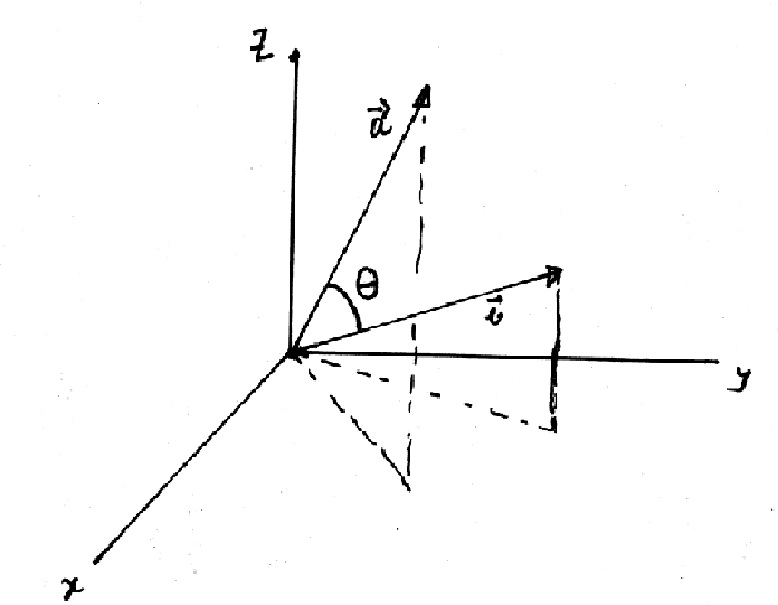
\includegraphics[width=100 mm]{euclid3vector.jpg}
\caption{A vector in the Euclidean three-space is represented by a directed line}
\end{figure}

\begin{flushleft}
The scalar product $(\psi_a,\psi_b)$ is the usual dot product
\end{flushleft}

\begin{align*}
\vec{a}.\vec{b} &= a_1 b_1 + a_2 b_2 + a_3 b_3 \\
               &= |\vec{a}| |\vec{b}| cos \theta
\end{align*}
where $|\vec{a}|$ and $|\vec{b}|$ are the magnitudes of the vectors $\vec{a}$ and $\vec{b}$ defined as

$$|\vec{a}| \equiv \sqrt{(\psi_a,\psi_a)} = \sqrt{a_1^2 + a_2^2 + a_3^2}$$
$$|\vec{b}| \equiv \sqrt{(\psi_b,\psi_b)} = \sqrt{b_1^2 + b_2^2 + b_3^2}$$


\section{Norm of a vector}

If a vector space is endowed with a scalar product, then the scalar product gives us the concept of the `magnitude' or `length' of a vector. In a general vector space the `magnitude' or `length' of a vector is called the norm of the vector. We simply define the norm of a vector $\psi_a$ as

$$\norm{\psi_a} \stackrel{def}{\equiv} \sqrt{(\psi_a,\psi_a)} $$

\begin{flushleft}
The norm has the following properties:
\end{flushleft}

\begin{description}
\item {\bf (a)} $\norm{\psi_a} \geq 0$, the equality holds only if the vector is null
\item {\bf (b)} $\norm{\psi_a + \psi_b} \leq \norm{\psi_a} + \norm{\psi_b}$, this is called the triangle inequality
\item {\bf (a)} $\norm{\psi_a - \psi_b} = \norm{\psi_b - \psi_a}$
\end{description}


\section{Metric induced by the scalar product}

The norm induced by the scalar product allows us to develop the concept of `distance' between vectors in a vector space. We say two vectors $\psi_a$ and $\psi_b$ are `close' if

$$\norm{\psi_a - \psi_b}$$
is small. The metric in a vector space assigns a real number to the vector $\psi_a - \psi_b$. This real number is a measure of how close the two vectors are. We simply define the metric $d(\psi_a,\psi_b)$ as

$$d(\psi_a, \psi_b) \stackrel{def}{\equiv} \norm{\psi_a - \psi_b}$$
Thus, if there are three vectors $\psi_a$, $\psi_b$ and $\psi_c$ and if $d(\psi_a,\psi_b) < d(\psi_a,\psi_c)$, then we say $\psi_a$ is closer to $\psi_b$ than to $\psi_c$.

\section{Schwarz inequality}

We will now prove a very important inequality called Schwarz inequality which states

\begin{flalign*}
&& \abs{(\psi_a, \psi_b)} &\leq \sqrt{(\psi_a, \psi_a)(\psi_b, \psi_b)}&\\
\text{or} && \abs{(\psi_a, \psi_b)} &\leq \norm{\psi_a} \norm{\psi_b}&\\
\end{flalign*}
{\bf Proof}

\begin{flalign*}
\text{Let}  && \psi        &= \psi_a + \lambda\psi_b &\\
\text{Then} && (\psi,\psi) &= (\psi_a + \lambda\psi_b, \psi_a+\lambda\psi_b)&\\
            &&             &= (\psi_a,\psi_a) + \lambda(\psi_a,\psi_b) + \lambda^\ast(\psi_b,\psi_a) + \abs{\lambda}^2(\psi_b,\psi_b) \geq 0
\end{flalign*}
The best inequality is obtained if $\lambda$ is chosen so as to minimize the left hand side of the above equation. By differentiation, the value of $\lambda$ which accomplishes this is found to be

$$\lambda = - \frac{(\psi_b,\psi_a)}{(\psi_b,\psi_b)}$$
Substitute this value of $\lambda$ in the above equation yields the Schwarz inequality. We note that the equality sign holds if and only if $(\psi,\psi) = 0$, i.e., $\psi$ is the null vector, i.e., $\psi = \phi$, in other words

\begin{flalign*}
&&\psi_a + \lambda\psi_b  &= \phi \text{ (null)}&\\
\text{i.e.} && \psi_a &= -\lambda\psi_b + \phi &\\
\text{or}   && \psi_a &= -\lambda\psi_b
\end{flalign*}
Hence, the equality holds if $\psi_a$ and $\psi_b$ are multiples of each other, or if $\psi_a$ and $\psi_b$ are ``parallel". It follows from the Schwarz inequality that the scalar product $(\psi_a,\psi_b)$ is finite if the norms of $\psi_a$ and $\psi_b$ are finite.

\section{Analogy of Schwarz inequality with vectors in a three-dimensional Euclidean space $\R^3$}

In $\R^3$, the vectors can be represented by directed lines (i.e., arrows). We have the scalar product of ordinary vectors in the form

$$\vec{A}.\vec{B} = \abs{\vec{A}}\abs{\vec{B}} \cos \theta.$$
Since cosine of any angle lies between -1 and 1, we have

$$\abs{\vec{A}.\vec{B}} \leq \abs{\vec{A}}\abs{\vec{B}}$$
The analogue of this equation for a general vector space is the Schwarz inequality:

$$\abs{(\psi_a, \psi_b)} \leq \norm{\psi_a} \norm{\psi_b}$$

% Done so far



\section{Orthogonality and linear independence}

A vector whose norm is unity is called a unit vector. For any given non-null vector, a unit vector can be formed by dividing the vector by its norm. Thus

$$u_a = \frac{\psi_a}{\norm{\psi_a}}$$
is normalized.

Two vectors $\psi_a$ and $\psi_b$ are orthogonal if their inner product is zero, i.e., if

$$(\psi_a,\psi_b) = 0.$$
The unit vectors $u_1$, $u_2$, ..., $u_N$ form an orthonormal set if they are mutually orthogonal, i.e., if

$$(u_i,u_j) = \delta_{ij}, \quad i,j = 1,2, \cdots , N.$$

\subsection{Linear Independence}

The set of vectors $\psi_1, \psi_2, \ldots , \psi_N$ are linearly independent if none of them can be expressed as a linear combination of the others. Mathematically this means that the equation

$$\sum_{j=1}^{N} c_j \psi_j = 0$$
cannot be satisfied except by $c_j = 0$ for all $j$.

\subsection{Orthonormality and linear independence}

A set of mutually orthogonal vectors (not necessarily normalized) are necessarily linearly independent. The converse is not true, however. That is, a set of linearly independent vectors may not be mutually orthogonal.

It is always possible to orthonormalize a set of linearly independent vectors. By this we mean that from a given set of $N$ linearly independent vectors, it is possible to form a set of $N$ orthonormal vectors. This procedure is called Schmidt orthonormalization method.



\subsection{Schmidt orthonormalization method}

Suppose $\psi_1, \psi_2, ..., \psi_N$ is a set of linearly independent vectors. Let
\be
u_1= \frac{\psi_1}{\norm{\psi_1}}.
\ee
Note that $u_1$ is normalized, i.e., $(u_1,u_1)=1$. Next construct the vector $\psi_{2}^{\prime}$ as follows:

\be
\psi_{2}^{\prime} = \psi_2 - u_1(u_1,\psi_2) ,
\ee
i.e., to obtain $\psi_{2}^{\prime}$ we have subtracted the `component' of $\psi_2$ along the $u_1$ ``direction''. Then it follows that
\begin{eqnarray*}
(u_1,\psi_2^{\prime}) &= &(u_1,\psi_2) - (u_1,u_1)(u_1,\psi_2) \\
                      &=& (u_1,\psi_2) - (u_1,\psi_2)       \\
                      &=& 0,
\end{eqnarray*}
i.e., $\psi_2^{\prime}$ is orthogonal to $u_1$. We then normalize $\psi_2^{\prime}$, i.e.,
\be
u_2 = \frac{\psi_2^{\prime}}{\norm{\psi_2^{\prime}}}.
\ee

\paragraph{}
We can continue the process until we exhaust all the vectors. For example, in the next step we can write
\be
\psi_3^{\prime} = \psi_3 - u_1(u_1,\psi_3) - u_2(u_2,\psi_3).
\ee
We note immediately that $\psi_3^{\prime}$ is orthogonal to both $u_1$ and $u_2$, i.e.,
$$(u_1, \psi_3^{\prime}) = (u_2,\psi_3^{\prime}) = 0$$
We normalize $\psi_3^{\prime}$ to get $u_3$, i.e.,
\be
u_3 = \frac{\psi_3^{\prime}}{\norm{\psi_3^{\prime}}}
\ee
Finally, in the $N^{th}$ step, we write
$$\psi_N^{\prime} = \psi_N - u_1(u_1,\psi_N) - u_2(u_2,\psi_N) - .... - u_{N-1}(u_{N-1},\psi_N)$$
$\psi_N^{\prime}$ is orthogonal to $u_1, u_2, ..., u_{N-1}$, i.e.,
$$(u_1,\psi_N^{\prime}) = (u_2,\psi_N^{\prime}) = ..... = (u_{N-1},\psi_N^{\prime}) = 0$$
Normalizing $\psi_N^{\prime}$ we get
\be
 u_N = \frac{\psi_N^{\prime}}{\norm{\psi_N^{\prime}}}.
\ee
Thus, the set $\{u_1,u_2,...,u_N\}$ is an orthonormal set of vectors.


% Done so far

\subsection{Dimension of a vector space}

The vector space $V$ is said to be $n$-dimensional if there exists $n$ linearly independent vectors, but if $n+1$ vectors are linearly dependent. The dimension may be finite or infinite.




\section{Complete vector space}

Before defining what a complete vector space is, we will give some other necessary definitions.

A sequence of vectors ${\psi_n}$ in the vector space $V$ is called a Cauchy sequence if for every $\epsilon > 0$ there exists 
an integer $N$ such that

$$\norm{\psi_n-\psi_m} < \epsilon$$
if $n,m>N$. In other words, the vectors in the sequence come `closer' if the index increases.

\begin{flushleft}
In particular
\end{flushleft}
$$\norm{\psi_n-\psi_m} \rightarrow 0 \text{ as } n,m \rightarrow \infty$$



\subsection{Convergence of a sequence of vectors in a vector space}

A sequence ${\psi_n},  n=1,2,...$ in a vector space $V$ converges to a vector $\psi$ in $V$ if for every $\epsilon > 0$ there exists an integer $N$ such that

$$\norm{\psi - \psi_n} < \epsilon$$
if $n>N$. That is, if

\begin{flalign*}
&& \lim_{n\rightarrow\infty}\norm{\psi - \psi_n} &= 0  &\\
\text{or} && {\psi_n} \rightarrow \psi,
\end{flalign*}
and the sequence is called a convergent sequence.

\noindent 
Now, we can show every convergent sequence is a Cauchy sequence.


\flushleft{\textbf{Proof}}
\begin{flalign*}
\text{Let}  && {\psi_n} &\rightarrow \psi &\\
\text{Then} && \norm{\psi_n-\psi_m} &= \norm{\psi_n-\psi+\psi-\psi_m}&\\
            &&                      &\leq \norm{\psi_n-\psi} + \norm{\psi-\psi_m} & \text{(triangle inequality)}
\end{flalign*}
Since $\{\psi_i, i=1,2, \cdots\}$ is a convergent sequence, each term on the right hand side tends to zero as $n$ and $m$ tends to infinity. 
Hence $\norm{\psi_n-\psi_m}\rightarrow 0$ as $n, m \rightarrow \infty$, i.e., the sequence $\{\psi_i, i=1,2,\cdots\}$ is a Cauchy sequence.


\paragraph{}
The converse of the above statement is not true in general. In other words, a Cauchy sequence in a vector space may not converge to a vector in the space. It can be shown that for a finite dimensional vector space the converse is true, i.e., in a finite 
dimensional vector space a Cauchy sequence is always a convergent sequence. Exceptions may arise in infinite dimensional vector space.




\subsection{An example of a vector space where Cauchy sequence does not converge to a vector in the vector space}

Consider the vector space consisting of all continuous functions of a single real variable $x$ in the range $[-1,1]$. In this vector space consider the
sequence $\{f_k(x), k = 1,2,\cdots\}$ of the following form:

\[
 f_k(x) = 
  \begin{cases} 
   1                    & \text{for } \frac{1}{k} \leq x \leq 1      \\
   \frac{kx+1}{2}       & \text{for } -\frac{1}{k} < x < \frac{1}{k} \\
   0                    & \text{for } -1 \leq x \leq -\frac{1}{k}
  \end{cases}
\]

$$k=1,2,3....$$

The graph of the sequence of functions is shown in Fig. (\ref{fig:sequence}) below.
\begin{figure}[ht!]
\centering
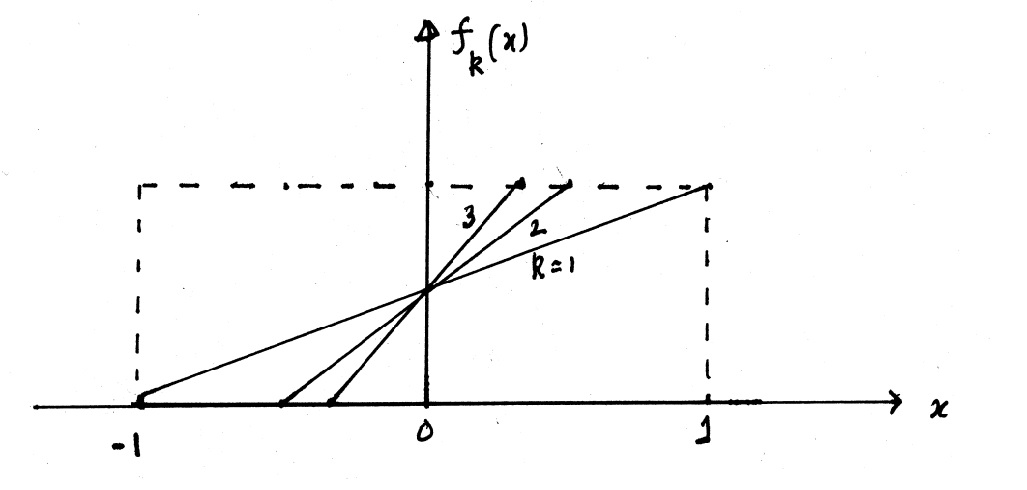
\includegraphics[width=\linewidth]{fig2.jpg}
\caption{A sequence of continuous functions converging to a discontinuous function}
\label{fig:sequence}
\end{figure}


Note that, in this example each $f_k(x)$ is continuous, but their first derivatives are discontinuous.

Let us define the scalar product in this space as

$$(f,g) = \int_{-1}^{+1} f^{\ast}(x) g(x) dx $$
so that the metric $d(f,g)$, i.e, the ``distance"   between the vectors $f$ and $g$ can be defined as
\[
d(f,g) \equiv || f-g || = \sqrt{ \int_{-1}^{+1} \left( f^*(x)-g^*(x)\right)\left( f(x)-g(x)\right) dx }. \]
With this metric we can show that the sequence $\{f_k\}$ defined above is indeed a Cauchy sequence. However, looking at the graph above, we see that as $k$ becomes large, $f_k$ approaches the $\theta$ function

\[
 \theta(x) = 
  \begin{cases} 
   0    & \text{for } x < 0 \\
   1    & \text{for } x > 0 \\
  \end{cases}
\]
which is a discontinuous function at $x=0$. We show the graph of $\theta(x)$ below
\begin{figure}[ht!]
\centering
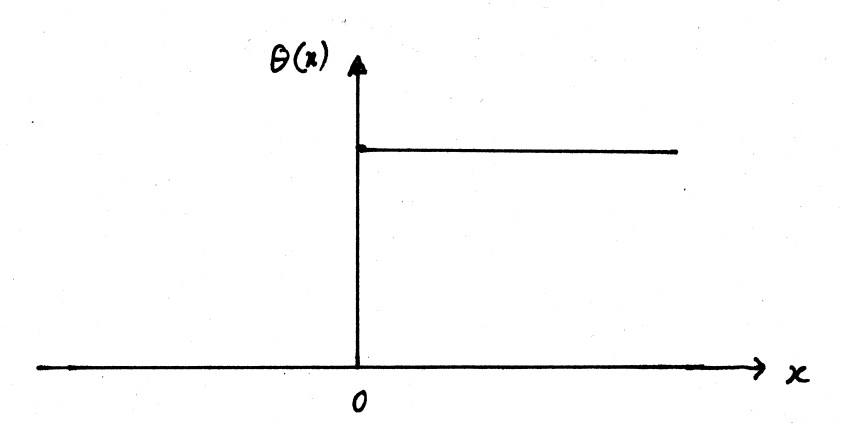
\includegraphics[width=80 mm]{theta.jpg}
\caption{The theta function.}
\end{figure}


Thus the Cauchy sequence $\{f_k(x)\}$ of continuous functions is converging to a discontinuous function which lies outside the vector space $V$ because the vector space was defined as the collection of all continuous functions.

\paragraph{}
If, instead of choosing all continuous functions, we had chosen all square integrable functions as defining the vector space, then any Cauchy sequence in the vector space would converge to a vector within the space.

\vspace{3 mm}
\textbf{Def: } A linear vector space is said to be \underline{complete} if any Cauchy sequence converges to a vector in the space.




\subsection{Hilbert Space}

A complete linear vector space, finite or infinite dimensional, endowed with a scalar product between vectors (and hence endowed with a norm and metric induced by the scalar product), is called a Hilbert space.

A finite-dimensional vector space is always complete. So, a finite-dimensional linear vector space in which a scalar product is defined is a Hilbert space.

An infinite dimensional vector space with a scalar product may or may not be complete. Whether or not an infinite-dimensional vector space is complete depends upon how exactly the vector space is defined and on the metric.

\section{Basis in a Hilbert space}

\subsection{Finite dimensional space}

In a finite dimensional vector space of dimension $n$, any set of  $n$ linearly independent vectors $\psi_1, \psi_2, ...., \psi_n$ spans the entire space. In other words, an arbitrary vector $\psi$ in the space can be expressed as a linear combination of $\psi_1, \psi_2, ...., \psi_n$, i.e.,

\be
\psi = \sum_{i=1}^{n} a_i \psi_i.
\ee
The vectors $\{ \psi_1, \psi_2, ...., \psi_n\}$ form a complete basis for the vector space. These vectors, even if linearly independent, may not be orthogonal to each other. It is more convenient to use a set of $n$ orthonormal vectors $\{ \phi_1, \phi_2, ...., \phi_n\}$ as the basis. Being orthogonal, the vectors 
$\{ \phi_1, \phi_2, ...., \phi_n \}$ are automatically linearly independent. The orthonormal set of basis vectors 
$\{\phi_i, i=1,2,...n\}$, can be constructed from the set $\{\psi_i,i=1,2, ...,n\}$ by using the Schmidt orthonormalization procedure.

\vspace{3mm}
\hspace{5mm}Choosing the orthonormal set as the basis, any vector $\psi$ in the vector space can be written as
\be
\psi = \sum_{i=1}^{n} a_i \phi_i 
\ee
where
\be
(\phi_i,\phi_j) = \delta_{ij}.
\label{eq:phi}
\ee
Using Eq. (\ref{eq:phi}), we have 
\be
a_i = (\phi_i,\psi).
\ee

%done so far

\subsection{Infinite-dimensional vector space}

In an infinite-dimensional vector space the number of basis vectors is infinity. Let $\{\phi_1,\phi_2,\phi_3,...\}$ be an infinite set of orthonormal basis vectors spanning the infinite-dimensional Hilbert space. This set of basis vectors is said to be \underline{complete} if \underline{any} vector $\psi$ in the Hilbert space can be expanded as a linear combination of the basis vectors, i.e.,

\be
\psi = \sum_{i=1}^{\infty} a_i \phi_i.
\label{eq:infsum}
\ee
In an infinite-dimensional vector space, choosing an infinite number of basis vectors may not ensure that the basis set is complete. It may so happen that there are other linearly independent vectors, may be infinite in number, which have been missed in the first choice of the basis vectors. Whenever we have an infinite sum, as in Eq. (\ref{eq:infsum}), the issue of convergence arises. We can understand
Eq. (\ref{eq:infsum}) in the sense that the sequences consisting of the partial sums
$$f_n = \sum_{i=1}^{n}a_i\phi_i \hspace{3mm} ; \hspace{3mm} n = 1, 2, 3,...$$
converges to $\psi$, i.e.,
\be
\lim_{n \rightarrow \infty} \norm{\psi - f_n} \rightarrow 0 
\ee
% Done so far
% need correction here
% what is limit of n?
Since the vector $\psi$ must have a finite norm, we must have
\be
\norm{\psi}^2 = (\psi,\psi) = \sum_{i=1}^{\infty} \abs{a_i}^2 < \infty \text{ (finite)} .
\label{eq:finite}
\ee
If the basis vectors $\phi_i$ are orthonormal, we have
$$a_i = (\phi_i, \psi),$$
so that Eq. (\ref{eq:finite}) can be written as
\be
\sum_{i=1}^{\infty}\abs{(\phi_i,\psi)}^2  < \infty .
\ee
The scalars $a_i$ can be regarded as the components of $\psi$ in the `directions' $\phi_i$.
\vspace{3mm}

%done so far

\underline{\textbf{Ex}}.  Show that the set of all square integrable functions, i.e., set of all functions $f$ such that 

$$\int_{-\infty}^{\infty} f^{\ast}(x)f(x)dx < \infty \text{  (i.e., finite)}$$
belong to a Hilbert space. This Hilbert space is denoted as $L^2(-\infty,\infty)$.

\vspace{3mm}

To show this, consider the following:

\begin{enumerate}
\item  If $f$ and $g$ are square integrable functions, so if $f+g$, and hence $f+g$ also belongs to the Hilbert space.
$$\norm{f+g} \leq \norm{f} + \norm{g}$$

\item  We can define the scalar product between $f$ and $g$ as follows:
$$(f,g) \stackrel{def}{\equiv} \int_{-\infty}^{\infty}f^{\ast}(x)g(x)dx$$
That the scalar product exists follows from the Schwarz inequality
$$\abs{(f,g)} \leq \norm{f}.\norm{g} < \infty$$

\item  It can also be shown that any Cauchy sequence of square integrable functions converges to a limit which is also square integrable. In other words, the space of all square integrable functions is complete.
\end{enumerate}

Hence the linear vector space consisting of all square integrable functions is indeed a Hilbert space.


% done so far

\section{Dirac Notation}
Cohen-Tannoudji, page 109. \newline
``Ket'' vectors a ``bra'' vectors. 
\vspace{3mm}

\textbf{\underline{Notation}}

\hspace{5mm}Any element, or vector of a vector space $V$ is called a \underline{ket vector}, or, more simply, a \underline{ket}. It is represented by the symbol $\ket{\hspace{1mm}}$, inside which is placed a distinctive sign which enables us to distinguish between different kets, for example $\ket{\psi}$.

\vspace{3mm}

\textbf{\underline{Scalar product}}

\vspace{1mm}

\hspace{5mm}With each pair of kets $\ket{\phi}$ and $\ket{\psi}$, taken in this order, we associate a complex number, which is their scalar product $(\ket{\phi}, \ket{\psi})$ and which satisfies various properties discussed earlier in section 
\ref{sec:innerproduct}.

\newpage

\textbf{\underline{Dual vector space}}

\vspace{1mm}

Linear functional:\newline
First we define the a linear functional. A linear functional $\chi$ is a linear operation on the kets such that $\chi$ operating on a ket $\ket{\psi}$ gives a complex scalar:
$$\chi \ket{\psi} \rightarrow \text{scalar, where } \ket{\psi} \in V$$
and
$$\chi (\lambda_1 \ket{\psi_1} + \lambda_2 \ket{\psi_2}) = \lambda_1 \chi \ket{\psi_1} + \lambda_2 \chi \ket{\psi_2}\text{.}$$
The set of all linear functionals defined on the kets of a vector space $V$ themselves form a linear vector space called the dual space of $V$ and symbolized by $V^{\ast}$.

\vspace{3mm}

\textbf{\underline{Bra notation for the vectors of $V^{\ast}$}}

\vspace{1mm}

\hspace{5mm}Any element, or vector, of the space $V^{\ast}$ is called a ``bra vector'', or, more simply, a bra. It is symbolized by $\bra{\hspace{1mm}}$. For example, the bra $\bra{\chi}$ designates the linear functional $\chi$. We shall henceforth use the notation $\braket{\chi}{\psi}$ to denote the number obtained by causing the linear functional $\bra{\chi} \in V^\ast$ to act on the ket $\ket{\psi} \in V$. Thus
$$\chi(\ket{\psi}) = \braket{\chi}{\psi}\text{.}$$




\textbf{\underline{Correspondence between kets and bras}}

\vspace{1mm}

\hspace{5mm}The existence of the scalar product in $V$ will now enable us to show that we can associate with every ket 
$\ket{\phi} \in V$ an element of $V^\ast$, that is a bra, which will be denoted by $\bra{\phi}$.

\hspace{5mm}The ket $\ket{\phi}$ does indeed enable us to define a linear functional, the one which associates with each $\ket{\psi} \in V$ a complex number which is equal to the scalar product $(\ket{\phi},  \ket{\psi})$. Let  $\bra{\phi}$ be this linear functional. It is thus defined by the relation
$$\braket{\phi}{\psi} = (\ket{\phi}, \ket{\psi})\text{.}$$


\newpage

\textbf{\underline{The correspondence is antilinear}}

\vspace{1mm}

Let $\lambda_1 \ket{\phi_1} +\lambda_2 \ket{\phi_2}$ be a ket. Then
\begin{flalign*}
&& (\lambda_1 \ket{\phi_1} +\lambda_2 \ket{\phi_2}, \ket{\psi}) &= \lambda_1^{\ast} (\ket{\phi_1},\ket{\psi}) + \lambda_2^{\ast} (\ket{\phi_1},\ket{\psi}) & \\
&& &= \lambda_1^{\ast} \braket{\phi_1}{\psi} + \lambda_2^{\ast} \braket{\phi_2}{\psi} & \\
&& &= (\lambda_1^{\ast}\bra{\phi_1} + \lambda_2^{\ast}{\bra{\phi_2}})\ket{\psi}
\end{flalign*}
Thus
$$\lambda_1 \ket{\phi_1} +\lambda_2 \ket{\phi_2}  \stackrel{dc}{\rightarrow} \lambda_1^{\ast}\bra{\phi_1} + \lambda_2^{\ast}{\bra{\phi_2}}$$
where ``dc'' is short for dual correspondence.

\vspace{3mm}

\textbf{\underline{Comment}}

\vspace{1mm}
\hspace{5mm} If $\lambda$ is a complex number and $\ket{\psi}$ is a ket, then $\lambda\ket{\psi}$ is also a ket. We are sometimes led to write $\lambda\ket{\psi}$ as $\ket{\lambda\psi}$:
$$\ket{\lambda\psi} = \lambda\ket{\psi}$$
One must be careful to remember that $\bra{\lambda\psi}$ represents the bra associated with the ket $\ket{\lambda\psi}$. Since the correspondence between a bra and a ket is antilinear, we have
$$\bra{\lambda\psi} = \lambda^\ast \bra{\psi}$$

\vspace{3mm}

\textbf{\underline{Dirac notation for the scalar product}}

\vspace{1mm}
\hspace{5mm} We now have at our disposal two distinct notations for designating the scalar product of $\ket{\psi}$ by 
$\ket{\phi}$, namely, $(\ket{\phi},\ket{\psi})$ and $\braket{\phi}{\psi}$, $\bra{\phi}$ being the bra associated with the ket $\ket{\phi}$.

We shall mostly use the Dirac notation $\braket{\phi}{\psi}$. In the table below we summarize, in Dirac notation, the properties of the scalar product:

\begin{enumerate}
\item  $\braket{\phi}{\psi} = \braket{\psi}{\phi}^\ast$
\item  $\braket{\phi}{\lambda_1\psi_1 + \lambda_2\psi_2} = \lambda_1\braket{\phi}{\psi_1} + \lambda_2 \braket{\phi}{\psi_2}$
\item  $\braket{\lambda_1\phi_1 + \lambda_2\phi_2}{\psi} = \lambda_1^\ast \braket{\phi_1}{\psi} + \lambda_2^\ast \braket{\phi_2}{\psi} $
\item  $\braket{\psi}{\psi} $ is real, positive; zero if and only if $\ket{\psi} = \phi $ (null).
\end{enumerate}

%%  Hooray











%References
%\begin{enumerate}
%	\item 
%	Quantum Mechanics	-	Shanker
%	
%	\item
%	Quantum Mechanics	- Sakurai
%\end{enumerate}
%
%\section{Definition}
%A linear vector space $V$ is a collection of objects $\psi_a, \psi_b, \ldots$, called vectors, which satisfy the following postulates:
%\begin{enumerate}
%	\item 
%	If $\psi_a$ and $\psi_b$ are vectors in $V$, there is a unique vector $\psi_a + \psi_b$ in $V$, called the sum of $\psi_a $ and $\psi_b$. In other words, and operation called addition is defined in the vector space such that the space is closed under addition.
%	
%	\item 
%	The vector addition is commutative and associative, i.e.,
%	\begin{eqnarray}\label{eqn:2.1-2.2}
%		\psi_a + \psi_b &= \psi_b + \psi_a \\
%		\psi_a + (\psi_b + \psi_c) &= (\psi_a + \psi_b) + \psi_c
%	\end{eqnarray}
%	
%	\item 
%	There is a vector in $V$ called the null vector and denoted by $\phi$ satisfying
%	\begin{equation}\label{eqn:2.3}
%	\psi_a + \phi = \phi + \psi_a
%	\end{equation}
%	for every $\psi_a$ in $V$.
%	
%	\item 
%	For every vector $\psi_a$ in $V$ there is another vector $\psi_a^\prime$ in $V$ such that
%	\begin{equation}\label{eqn:2.4}
%	\psi_a + \psi_a^\prime = \phi
%	\end{equation}
%	we denote $\psi_a^\prime$ as $-\psi_a$.\\
%	(Note : we use the notation $\psi_a - \psi_b$ to mean $\psi_a + (-\psi_b$).
%	
%	\item 
%	If $\psi_a$ is a vector and $\lambda$ is an arbitrary number (real or complex), called a scaler, there is a uniquely defined vector $\lambda \psi_a$ in $V$ satisfying.
%	\begin{enumerate}
%		\item 
%		\begin{equation}\label{eqn:2.5}
%		\lambda (\psi_a  + \psi_b) = \lambda \psi_a + \lambda + \psi_b
%		\end{equation}
%		i.e., multiplication is distributive with respect to vector addition.
%		
%		\item 
%		\begin{equation}\label{eqn:2.6}
%		(\lambda \mu) \psi_a = \lambda (\mu \psi_a)
%		\end{equation}
%		i.e., multiplication  by a scalar is associative.
%		
%		\item 
%		\begin{equation}\label{eqn:2.7}
%		(\lambda + \mu) \psi_a = \lambda \psi_a + \mu \psi_b
%		\end{equation}
%		i.e., multiplication is distributive with respect to addition scalars.
%		
%		\item 
%		Multiplication by scalars $0$ and $1$ are defined by
%		\begin{eqnarray}\label{eqn:2.8-2.9}
%			0 \psi_a = \phi \\
%			1 \psi_a = \psi_a
%		\end{eqnarray}
%		for any $\psi_a$ in $V$.
%	\end{enumerate}
%\end{enumerate}
%\section{Example of linear vector space}
%\begin{enumerate}
%	\item 
%	Consider all real numbers $x$ in the range $-\infty$ to $\infty$, i.e.,
%	\begin{eqnarray}\label{eqn:2.10-2.11}
%		-\infty < x < \infty \\
%		x \in \Re \ \ \text{ ($\Re$ is the set of all real numbers )}
%	\end{eqnarray}
%	Take any two real numbers $x_1$ and $x_2$. If we add two real numbers we get another real number in $\Re$. Thus
%	\begin{equation}\label{eqn:2.12}
%	x_1 + x_2 = \Re
%	\end{equation}
%	Next take any real number $x$. If we multiply $x$ by another real number $\lambda$, we get a real number in $\Re$, i.e.,
%	\begin{equation}\label{eqn:2.13}
%	\lambda x \in \Re
%	\end{equation}
%	If we take a real number $x$, then there exists another real number $-x$ such that
%	\begin{equation}\label{eqn:2.14}
%	x + (-x) = 0
%	\end{equation}
%	So the real numbers form a vector space with the real numbers themselves as vectors in the space. The number $0$ is the null vector $\phi$ of the  space. The scalars $\lambda$ by which the vectors are multiplied are also real numbers.\\
%	Thus the real numbers form a real linear vector space over a field which are also real numbers. The addition and multiplication are just the normal addition and multiplication of the real numbers.
%	
%	\item 
%	The set of $n-tuples$ of numbers $(x_1, x_2, \ldots, x_n)$.
%	When the addition of vectors and multiplication by a scalar are defined by
%	\begin{equation}\label{eqn:2.15}
%	(x_1 , x_2, \ldots, x_n) + (y_1 , y_2, \ldots, y_n) = (x_1 + y_1, x_2 + y_2, \ldots, x_n + y_n)
%	\end{equation}
%	and 
%	\begin{equation}\label{eqn:2.16}
%	\lambda (x_1, x_2, \ldots, x_n) = (\lambda x_1, \lambda x_2, \ldots, \lambda x_n)
%	\end{equation}
%	
%	
%	\item 
%	The collection of all square-integrable complex valued functions of a real variable form a vector space. consider all functions
%	\begin{equation}\label{eqn:2.17}
%	f:\Re \rightarrow \mathbb{C}
%	\end{equation}
%	here, 
%	$\Re $ =  set of real numbers \\
%	$\mathbb{C}$  = set of complex numbers\\
%	such that
%	\begin{equation}\label{eqn:2.18}
%	\int_{-\infty}^{\infty} f^*(x) f(x) dx \equiv \int_{-\infty}^{\infty} |f(x)|^2 dx < \infty \text{\  \ (i.e., finite)}
%	\end{equation}
%	The sum of two functions and the product of a function by a complex scalar are defined in the usual way.\\
%	The reason the square-integrable functions form a (complex) vector space is that the space is closed under addition. The vectors of the space are the square-integrable functions. In other words, it can be shown that if $f$ and $g$ are two vectors, in this case two functions $f(x)$ and $g(x)$ both of which are square integrable, then $f(x) + g(x)$ is also square integrable and have the sum belong to the vector space.\\
%	\textbf{proof:} \\
%	Let $f(x)$ and $g(x)$ be two square integrable function, i.e., 
%	\begin{equation}\label{eqn:2.19}
%	\int_{-\infty}^{\infty} |f(x)|^2 dx < \infty
%	\end{equation}
%	and
%	\begin{equation}\label{eqn:2.20}
%	\int_{-\infty}^{\infty} |g(x)|^2 dx < \infty
%	\end{equation}
%	then using the inequality
%	\begin{equation}\label{eqn:2.21}
%	\int_{-\infty}^{\infty} |f+g|^2 dx \leq \left[\sqrt{\int_{\infty}^{\infty} |f|^2 dx} \sqrt{\int_{\infty}^{\infty} |g|^2 dx}\right]^2
%	\end{equation}
%	it is obvious that
%	\begin{equation}\label{eqn:2.22}
%	\int_{-\infty}^{\infty} |f+g|^2 dx < \infty
%	\end{equation}
%	(i.e., finite).
%	
%	\item 
%	The set of all $n\times n$ matrices with complex elements form a complex linear vector space. For illustation let us take $2\times 2$ matrix $A$
%	\begin{equation}\label{eqn:2.23}
%	A = \left(			
%	\begin{matrix}
%	a & b \\
%	c & d
%	\end{matrix}
%	\right)
%	\end{equation}
%	where the elements $a, b, c$ and $d$ can, in general, be complex. Then $A$ belongs to a vector (complex) space.
%	We have
%	
%	\begin{eqnarray}\label{eqn:2.24-2.27}
%		\phi &= \left(
%		\begin{matrix}
%			0 & 0 \\ 0 & 0
%		\end{matrix}
%		\right)\\
%		\mathbb{I} &= \left(
%		\begin{matrix}
%			1 & 0 \\ 0 & 1
%		\end{matrix}
%		\right)\\
%		-A &= \left(
%		\begin{matrix}
%			-a & -b \\ -c & -d
%		\end{matrix}
%		\right)\\
%		\lambda A &= \left(
%		\begin{matrix}
%			\lambda a & \lambda b \\ \lambda c & \lambda d
%		\end{matrix}
%		\right)
%	\end{eqnarray}
%	The set of all these matrices form a vector space.						
%\end{enumerate}
%
%\section{Inner product space or a unitary vector space}\label{inner_product}
%For a general linear vector space, product of vectors (i.e. multiplication of two vectors) need ot be defined. However, we will restrict ourselves to spaces in which a  scalar product or an inner product is defined.\\
%A linear vector space is called unitary if a scalar product is defined in it. To every pair of vectors $\psi_a$ and $\psi_b$ in $V$ there corresponds a unique scalar (in general complex), called the scalar product. The scalar product is defined to have the following properties :
%\begin{eqnarray}\label{eqn:2.28-2.32}
%	(\psi_a , \psi_b) &= (\psi_b, \psi_a)^* \\
%	(\psi_a , \lambda \psi_b) &= \lambda (\psi_a , \psi_b) \\
%	(\lambda \psi_a , \psi_b) &= \lambda^* (\psi_a , \psi_b) \\
%	(\psi_a , \psi_b + \psi_c) &= (\psi_a , \psi_b) + (\psi_a , \psi_c) \\
%	(psi_a, \psi_a) \geq 0 \ \text{;the equality holds only if $\psi_a$ is the null vector}
%\end{eqnarray}
%It follows from the above postulated properties of the scalar product, that the scalar product is linear with respect to post factors, i.e.,
%\begin{equation}\label{eqn:2.33}
%(\psi_a, \lambda \psi_b + \mu \psi_c) = \lambda (\psi_a , \psi_b) + \mu (\psi_a , \psi_c)
%\end{equation}
%and anti-linear with respect to the pre factors, i.e.,
%\begin{equation}\label{eqn:2.34}
%(\lambda \psi_a + \mu \psi_b, \psi_c ) = \lambda^* (\psi_a , \psi_c) + \mu^* (\psi_b , \psi_c)
%\end{equation}
%
%\section{Examples of scalar product}
%\begin{enumerate}[label=\textbf{Example \arabic*},start=1]
%	\item 
%	Consider the vector space consisting of all square integrable functions of a real variable in the domain $[a,b]$. This space is denoted by $L^2[a,b]$.\\
%	Suppose
%	\begin{equation}\label{eqn:2.35}
%	f \in L^2[a,b]
%	\end{equation}
%	i.e.,
%	\begin{equation}\label{eqn:2.36}
%	\int_{a}^{b} f^*(x)f(x) dx \equiv \int_{a}^{b} |f(x)|^2 dx < \infty
%	\end{equation}
%	We can define the scalar product of two vectors $f$ and $g$ as
%	\begin{equation}\label{eqn:2.37}
%	(f, g) _\equiv^{def} \int_{a}^{b} f^*(x) g(x) dx = complex \ number
%	\end{equation}
%	We can show
%	\begin{equation}\label{eqn:2.38}
%	\left|(f, g)\right| = \left[\sqrt{\int_{a}^{b} |f(x)|^2 dx}\right] \left[\sqrt{\int_{a}^{b} |g(x)|^2 dx}\right]
%	\end{equation}
%	Since both $f$ and $g$ are square integrable, $|(f, g)|$ is finite, i.e., the scalar product of $f$ and $g$ exists.\\
%	The scalar product defined above satisfies all the properties that a scalar product is postulated to have.
%	
%	
%	\item 
%	Now consider the vector space consisting of $n-tuples$ of complex numbers. Such a vector space is denoted as $\mathbb{C}^n$.\\
%	A vector $\psi_a \in \mathbb{C}^n$ may be expressed as
%	\begin{equation}\label{eqn:2.39}
%	\psi_a = \left(
%	\begin{matrix}
%	a_1 & a_2 & \ldots & a_n
%	\end{matrix}
%	\right)^T
%	\end{equation}
%	The scalar product may then be defined as
%	\begin{eqnarray}\label{eqn:2.40-2.41}
%		(\psi_a , \psi_b) &_\equiv^{def} \left(
%		\begin{matrix}
%			a_1^* & a_2^* & \ldots &  a_3^*
%		\end{matrix}
%		\right)\left(
%		\begin{matrix}
%			b_1 \\ b_1 \\ \vdots \\ b_n
%		\end{matrix}
%		\right)\\
%		&= \sum_{i=1}^{n} a_i^* b_i
%	\end{eqnarray}
%	This scalar product also satisfies all the properties of a scalar product.
%	
%	
%	\item 
%	Euclidean 3-space $\mathbb{R}^3$. The vectors of $\mathbb{R}^3$ are $3-tuples$ of real numbers which could be represented as column vectors . Thus if $psi_a$ and $\psi_b$ are in $\mathbb{R}^3$,
%	\begin{eqnarray}\label{eqn:2.42-2.43}
%		\psi_a &= \left(
%		\begin{matrix}
%			a1 \\ a2 \\ a3
%		\end{matrix}
%		\right)\\
%		\psi_b &= \left(
%		\begin{matrix}
%			b1 \\b2 \\b3
%		\end{matrix}
%		\right)
%	\end{eqnarray}
%	where $a_i$ and $b_i$ are real. \\
%	We could define the scalar product of $\psi_a$ and $\psi_b$ as
%	\begin{eqnarray}\label{eqn:2.44-2.46}
%		(\psi_a, \psi_b) &_\equiv^{def} 
%		\left(
%		\begin{matrix}
%			a_1 & a_2 & a_3
%		\end{matrix}
%		\right)\left(
%		\begin{matrix}
%			b_1 \\ b_2 \\ b_3
%		\end{matrix}
%		\right) \\
%		&= \psi_a^T \psi_b \\
%		&- \sum_{i=1}^{3} a_i b_i
%	\end{eqnarray}
%	This scalar product also has all the postulated properties of a scalar product.\\
%	
%	In case of the vector space $\mathbb{R}^3$, the vectors $\psi_a$ and $\psi_b$ could be represented as directed lines $\vec{a}$ and $\vec{b}$ in a three dimensional coordinate system.\\
%	
%	\textbf{figure}
%	\\
%	The Scalar product $(\psi_a, \psi_b)$ is the usual dot product
%	\begin{eqnarray}\label{eqn:2.47-2.48}
%		\vec{a} . \vec{b} &= a_1 b_1 + a_2 b_2 + a_3 b_3 \\
%		&= |\vec{a}||\vec{b}| \cos(\theta)
%	\end{eqnarray}
%	Where $|\vec{a}|$ and $|\vec{b}|$ are the magnitudes of the vectors $\vec{a}$ and $\vec{b}$ defined as
%	\begin{eqnarray}\label{eqn:2.49-2.50}
%		|\vec{a}| &\equiv \sqrt{(\psi_a , \psi_a)} = \sqrt{a_1^2 + a_2^2 + a_3^2} \\
%		|\vec{b}| &\equiv \sqrt{(\psi_b, \psi_b)} = \sqrt{b_1^2 + b_2^2 + b_3^2}
%	\end{eqnarray}
%	
%\end{enumerate}
%\section{Norm of a vector}
%If a vector space is enclosed with a scalar product, then the scalar product gives us the concept of the "magnitude" or "length" of a vector. In a general vector space the "magnitude" or "length" of a vector is called the norm of the vector. We simply define the norm of a vector $\psi_a$ as
%\begin{equation}\label{eqn:2.51}
%||\psi_a|| _\equiv^{def} \sqrt{(\psi_a, \psi_a)}
%\end{equation}
%The norm has the following properties:
%\begin{enumerate}
%	\item 
%	\begin{equation}\label{eqn:2.52}
%	||\psi_a|| \geq 0
%	\end{equation}
%	the equality holds only if the vector is null.
%	
%	\item 
%	\begin{equation}\label{eqn:2.53}
%	||\psi_a + \psi_b|| \leq ||\psi_a|| + ||\psi_b||
%	\end{equation}
%	This is called the triangle inequality
%	
%	\item 
%	\begin{equation}\label{eqn:2.54}
%	||\psi_a - \psi_b|| = ||\psi_b - \psi_a||
%	\end{equation}
%\end{enumerate}
%
%\section{Metric included by the scalar product}
%The norm included by the scalar product allows us to develop the concept of "distance" between vectors in a vector space. We say two vectors $\psi_a$ and $\psi_b$ are 'close' if $||\psi_a - \psi_b||$ is small. The metric in a vector space assigns a real number to the vector $\psi_a - \psi_b$. This real number is a measure of how close the two vectors are. We simply define the metric $\mathbf{d}(\psi_a, \psi_b)$ as
%\begin{equation}\label{eqn:2.55}
%\mathbf{d}(\psi_a, \psi_b) _\equiv^{def} ||\psi_a - \psi_b||
%\end{equation}
%Thus, if there are three vectors $\psi_a$, $\psi_b$ and $\psi_c$ and if $\mathbf{d}(\psi_a, \psi_b) < \mathbf{d}(\psi_a, \psi_c)$ then we say $\psi_a$ is closer to $\psi_b$ than to $\psi_c$.
%
%\section{Schwarz's inequality}
%We will now prove a very important inequality called Schwarz inequality which states
%\begin{equation}\label{eqn:2.56}
%|(\psi_a, \psi_b)| \leq \sqrt{(\psi_a, \psi_a)(\psi_b, \psi_b)}
%\end{equation}
%or
%\begin{equation}\label{eqn:2.57}
%|(\psi_a, \psi_b)| \leq ||\psi_a ||\ ||\psi_b||
%\end{equation}
%\textbf{proof : }
%Let
%\begin{equation}\label{eqn:2.58}
%\psi = \psi_a + \lambda \psi_b
%\end{equation}
%Then
%\begin{eqnarray}\label{eqn:2.59-2.60}
%	(\psi, \psi) &= (\psi_a + \lambda \psi_b, \psi_a + \lambda \psi_b) \\
%	&= (\psi_a, \psi_a) + \lambda (\psi_a, \psi_b) + \lambda^* (\psi_b, \psi_a) + |\lambda|^2 (\psi_b, \psi_b) \geq 0
%\end{eqnarray}
%The best inequality is obtained if $\lambda$ is chosen so as to minimize the left hand side of the above equation. By differentiation, the value of $\lambda$ which accomplishes this is found to be
%\begin{equation}\label{eqn:2.61}
%\lambda = - \frac{(\psi_b, \psi_a)}{\psi_b, \psi_b}
%\end{equation}
%Substituting this value of $\lambda$ in the above equation yields the Schwarz inequality.\\
%
%We note that the equality sign holds if and only if $(\psi, \psi) = 0$, i.e., $\psi$ is the null vector, i.e., $\psi = \phi$, in other words
%\begin{equation}\label{eqn:2.62}
%\psi_a + \lambda \psi_b = \phi (null)
%\end{equation}
%i.e.,
%\begin{eqnarray}\label{eqn:2.63-2.64}
%	\psi_a &= - \lambda \psi_b + \phi \\
%	\psi_a &= -\lambda \psi_b
%\end{eqnarray}
%Hence, the equality holds if $\psi_a$ and $\psi_b$ are multiple of each other, or if $\psi_a$ and $\psi_b$ are "parallel".\\
%It follows from the Schwarz inequality that the scalar product $(\psi_a, \psi_b)$ is finite if the norms of $\psi_a$ and $\psi_b$ are finite.
%
%\section{Analogy of Schwarz inequlity with vectors in a three-dimensional Euclidean space $\mathbb{R}^3$}
%In $\mathbb{R}^3$, the vectors can be represented by directed lines (i.e. arrows). We have the scalar product ordinary vectors in the form
%\begin{equation}\label{eqn:2.65}
%\vec{A} . \vec{B} = |\vec{A}| \ |\vec{B}| \cos(\theta)
%\end{equation}
%Since cosine of any angle lies between $-1$ and $+1$, we have
%\begin{equation}\label{eqn:2.66}
%|\vec{A} . \vec{B} | \leq |\vec{A}| \ |\vec{B}|
%\end{equation}
%The analogue of this equation for a general vector space is the Schwarz inequality
%\begin{equation}\label{eqn:2.67}
%|(\psi_a, \psi_b)| \leq ||\psi_a|| \ ||\psi_b||
%\end{equation}
%
%
%\section{Orthogonality and linear independence}
%A vector whose norm is unity is called a unit vector. For any given non-null vector, a unit vector can be formed by defining the vector by its norm. Thus
%\begin{equation}\label{eqn:2.68}
%u_a = \frac{\psi_a}{||\psi_a||}
%\end{equation}
%is normalized.\\
%Two vectors $\psi_a$ and $\psi_b$ are orthogonal if their inverse product is zero, i.e., if
%\begin{equation}\label{eqn:2.69}
%(\psi_a, \psi_b ) = 0
%\end{equation}
%The unit vectors $u_1, u_2, \ldots, u_N$ form an orthogonal set if they are mutually orthonormal , i.e., 
%\begin{equation}\label{eqn:2.70}
%(u_i, u_j) = \delta_{ij}
%\end{equation}
%
%\subsection{Linear independence}
%The set of vectors $\psi_1, \psi_2, \ldots, \psi_N$ are linearly independent if none of them can be expressed as a linear combination of the others. Mathematically this means that the equation
%\begin{equation}\label{eqn:2.71}
%\sum_{j=1}^{N} c_j \psi_j = 0
%\end{equation}	
%cannot be satisfied except by $c_j = 0$ for all $j$.
%
%\section{Orthonormality and linear independence}
%A dot of mutually orthogonal vectors (not necessarily normalized) are necessarily linearly independent. The converse is not true, however. That is, a set of linearly independent vectors may not be mutually orthogonal.\\
%It  is always possible to orthonormalize a set of linearly independent vectors. By this we mean that from a given set of $N$ linearly independent vectors, it is possible to form a set of $N$ orthonormal vectors. This procedure is called \textbf{Schmidt orthonormalization method}.
%
%\section{Schmidt orthonormalization method}
%\label{chapter2.schmidt-orthonormalization-method}
%Suppose $\psi_1, \psi_2, \ldots, \psi_N$ is a set of linearly independent vectors. Let
%\begin{equation}\label{eqn:2.72}
%u_1 = \frac{\psi_1}{||\psi_1||}
%\end{equation}
%Then $(u_1, u_1) = 1$, i.e., $u_1$ is normalized. Next construct the vector $\psi_2^\prime$ as follows:
%\begin{equation}\label{eqn:2.73}
%\psi_2^\prime = \psi_2 - u_1(u_1, \psi_2)
%\end{equation}
%i.e., to obtain $\psi_2^\prime$ we have subtracted the 'component' of $\psi_2$ along the $u_1$ "direction". Then it follows that
%\begin{eqnarray}\label{eqn:2.74-2.76}
%	(u_1, \psi_2^\prime) &= (u_1, \psi_2) - (u_1, u_1)(u_1, \psi_2) \\
%	&= (u_1, \psi_2) - (u_1, \psi_2) \\
%	&= 0
%\end{eqnarray}
%i.e., $\psi_2^\prime$ is orthogonal to $u_1$. We then normalize $\psi_2^\prime$, i.e.,
%\begin{equation}\label{eqn:2.77}
%u_2 = \frac{\psi_2^\prime}{||\psi_2^\prime ||}
%\end{equation}
%We can continue the process until we exhaust all the vectors. For example, in the next step we can write
%\begin{equation}\label{eqn:2.78}
%\psi_3^\prime = \psi_3 - u_1 (u_1, \psi_3) - u_2 (u_2, \psi_3)
%\end{equation}
%We note immediately that $\psi_3^\prime$ is orthogonal to both $u_1$ and $u_2$, i.e.,
%\begin{equation}\label{eqn:2.79}
%(u_1, \psi_3^\prime) = (u_2, \psi_3^\prime) = 0
%\end{equation}
%We normalize $\psi_3^\prime$ to get $u_3$, i.e.,
%\begin{equation}\label{eqn:2.80}
%u_3 = \frac{\psi_3^\prime}{||\psi_3^\prime ||}
%\end{equation}
%Finally, in the $N-th$ step, we write
%\begin{equation}\label{eqn:2.81}
%\psi_N^\prime = \psi_N - u_1(u_1, \psi_N) - u_2(u_2, \psi_N) - \ldots - u_{N-1}(u_{N-1}, \psi_N)
%\end{equation}
%$\psi_N^\prime$ is orthogonal to $u_1, u_2, \ldots, u_{N-1}$, i.e.,
%\begin{equation}\label{eqn:2.82}
%(u_1, \psi_N^\prime) = (u_2, \psi_N^\prime) = \ldots = (u_{N-1}, \psi_N^\prime) = 0
%\end{equation}
%Normalizing $\psi_N^\prime$ we get
%\begin{equation}\label{eqn:2.83}
%u_N = \frac{\psi_N^\prime}{||\psi_N^\prime ||}
%\end{equation}
%Thus, the set $\{u_1, u_2, \ldots, u_N\}$ is an orhtonormal set of vectors.
%
%\section{Dimension of a vector space}
%The vector space $V$ is said to be n-dimensional if there exists $n$ linearly independent vectors, but if $n+1$ vectors are linearly dependent the dimension may be finite or infinite.
%
%\section{Complete vector space}
%Before defining what a complete vector space is we will give some other definitions.\\
%A sequence of vectors $\{\psi_n\}$ in the vector space $V$ is called a \textbf{Cauchy sequence} if for every $\epsilon > 0$ there exists an integer $N$ such that
%\begin{equation}\label{eqn:2.84}
%||\psi_n - \psi_m || < \epsilon
%\end{equation}
%if $n, m > N$. In other words, the vectors in the sequence come 'closer' if the index increases. In particular
%\begin{equation}\label{eqn:2.85}
%||\psi_n - \psi_m || \rightarrow 0 \ as \ n,m \rightarrow \infty
%\end{equation}
%
%\section{Convergence of a sequence of vectors in a vector space}
%A sequence $\{\psi_n\}$ , $n = 1, 2, \ldots$ in a vector space $V$ converses to a vector $\psi$ in $V$ if for every $\epsilon > 0$ there exists an integer $N$ such that
%\begin{equation}\label{eqn:2.86}
%||\psi_n - \psi_m || < \epsilon
%\end{equation}
%if $n > N$, that is if
%\begin{equation}\label{eqn:2.87}
%\lim\limits_{n\rightarrow \infty} ||\psi - \psi_n|| = 0
%\end{equation}
%then 
%\begin{equation}\label{eqn:2.88}
%\{\psi_n \} \rightarrow \psi
%\end{equation}
%and the sequence is called a convergent sequence.\\
%Now we can show every convergent sequence is a Cauchy sequence.\\
%\textbf{proof}\\
%Let $\{\psi_n \} \rightarrow \psi$. Then
%\begin{eqnarray}\label{eqn:2.89-2.90}
%	|| \psi_n - \psi_m || &= ||\psi_n - \psi + \psi -\psi_m|| \\
%	&\leq ||\psi_n - \psi|| + ||\psi -\psi_m||
%\end{eqnarray}
%here the triangle inequality is used.\\
%Since $\{\psi_n \}$ is a convergent sequence, each term on the right hand side tends to zero as $n$ and $m$ tends to infinity. Hence $||\psi_n - \psi_m|| \rightarrow 0$ as $n,m=\infty$, i.e., the sequence $\{\psi_i\}$ with $i=1,2,\ldots$ is a Cauchy sequence.\\
%The converse of the above statement is not true in general. In other words, \textit{a Cauchy sequence in a vector space may not converge to a vector in the space}. It can be shown that for a finite dimensional vector space the conver is true, i.e., in a finite dimensional vector space a Cauchy sequence is always a convergent sequence. Exceptions may arise in infinite-dimensional vector space.
%
%\subsection{An example of a vector space whose Cauchy sequence does not converse to a vector in the vector space}
%Consider the vector space consisting of all continuous function of a single real variable $x$ in the range $[-1, 1]$. In this vector space consider a sequence $\{f_k (x) \}$, $k = 1,2,\ldots$ of the following form:
%\begin{equation}\label{eqn:2.91}
%f_k(x) = \begin{cases}
%1 \ \text{ for } \frac{1}{k} \leq x \leq 1 \\
%\frac{k x + 1}{2} \ \text{ for } \ -\frac{1}{k} < x < \frac{1}{k} \\
%0 \ \text{ for } \ -1 \leq x \leq - \frac{1}{k}
%\end{cases}
%\end{equation}
%$k = 1, 2, 3, \ldots$\\
%The graph of the sequence of functions is shown below:
%\\	
%% figure
%\textbf{figure}
%\\
%Note that,  in this example each $f_k(x)$ is continuous, but their first derivatives are discontinuous.\\
%
%Let us define the scalar product in this space as
%\begin{equation}\label{eqn:2.92}
%(f, g) = \int_{-1}^{1} f^*(x) g(x) dx
%\end{equation}
%So that the metric $\mathbf{d}(f, g)$, i.e., the "distance" between vectors $f$ and $g$ can be defined as
%\begin{eqnarray}\label{eqn:2.93-2.94}
%	\mathbf{d}(f, g) &\equiv ||f-g|| \\
%	&= \sqrt{\int_{-1}^{+1}\left(f^*(x) - g^*(x)\right)\left(f(x) - g(x)\right) dx}
%\end{eqnarray}
%With this metric we can show that the sequence ${f_k}$ defined above is indeed a Cauchy sequence. However, looking at the graph above, we see that as $k$ becomes large, $f_k$ approaches the $\theta$ function
%\begin{equation}\label{eqn:2.95}
%\theta(x) = 
%\begin{cases}
%0 \ \text{ for } \ x < 0 \\
%1 \ \text{ for } \ x > 0
%\end{cases}
%\end{equation}
%Which is a discontinuous function at $x=0$.\\
%We show that graph of $\theta(x)$ below:
%\\
%%figure
%\textbf{figure}
%\\
%Thus the Cauchy sequence $\{f_k(x) \}$ of continuous function is converging to a discontinuous function which lies outside the vector space $V$.\\
%If, instead of chooding all continuous function, we had chosen all square integrable function as defining the vector space, then any Cauchy sequence in the vector space would converge to a vector in the space.\\
%\textbf{Definition : } A linear vector space is said to be \underline{complete} if any Cauchy sequence converges to a vector in the space.
%
%\section{Hilbert space}
%A complete linear vector space, finite or infinite dimensional, ( and hence \textbf{@@@enclosed@@@} with  a norm and metric induced by the scalar product), is called a Hilbert space.\\
%A finite-dimensional vector space is always complete. So, a finite dimensional linear vector space in which a scalar product is defined is a Hilbert space.\\
%An infinite dimensional vector space with a scalar product may or may not be complete. Whether or not an infinite dimensional vector space is complete depends upon how exactly the vector space is defined and on the metric.
%
%\section{Basis vectors in a Hilbert space}
%\subsection{Finite dimensional space}
%In a finite dimensional vector space of dimension $n$, any set of linearly independent vectors $\psi_1, \psi_2, \ldots, \psi_n$ spans the entire space. In other words any vector $\psi$ in the space can be expressed as linear combination of $\psi_1, \psi_2, \ldots, \psi_n$, i.e.,
%\begin{equation}\label{eqn:2.96}
%\psi = \sum_{i=1}^{n} a_i \psi_i
%\end{equation}
%The vectors $\psi_1, \psi_2, \ldots, \psi_n$ form a complete basis for the vector space. The vectors $\psi_1, \psi_2, \ldots, \psi_n$, even if linearly independent, may not be orthogonal to each other. It is more convenient to use a set of orthonormal vectors $\phi_1, \psi_2, \ldots, \phi_n$ as the basis. Being orthogonal, the vectors $\phi_1, \psi_2, \ldots, \phi_n$ are automatically linearly independent. The orthonormal set of basis vectors $\{\phi_i \}$ $i = 1,2,\ldots,n$ can be constructed from the set $\{\psi_i \}$ $i = 1,2,\ldots,n$ by using the schmidt orthonormalization procedure.\\
%Choosing the orthonormal set as the basis, any vector $\psi$ in the vector space can be written as
%\begin{equation}\label{eqn:2.97}
%\psi = \sum_{i=1}^{n} a_i \phi_i
%\end{equation}
%where
%\begin{equation}\label{eqn:2.98}
%(\phi_i, \phi_i) = \delta_{ij}
%\end{equation}
%using equation \ref{eqn:2.98} we have
%\begin{equation}\label{eqn:2.99}
%a_i = (\phi_i, \psi)
%\end{equation}
%\subsection{Infinite dimensional vector space}
%In an infinite dimensional vector space the number of basis vectors is infinity. Let $\{\phi_1, \phi_2, \ldots \}$ be an infinite set of orthonormal basis vectors spanning the infinite dimensional Hilbert space. This set of basis vectors is said to be \underline{complete} if \underline{any} vector $\psi$ in the Hilbert space  can be expanded as a linear combination of the basis vectors, i.e.,
%\begin{equation}\label{eqn:2.100}
%\psi = \sum_{i=1}^{\infty} a_i \phi_i
%\end{equation}
%In an infinite dimensional vector space, choosing an infinite number of basis vectors may not ensure that the basis set is complete. It may so happen that there are other linearly independent vectors, may be infinite in numbers, which have been missed in the first choice of the basis vectors.\\
%Whenever we have an infinite sum, as in equation \ref{eqn:2.100} is to be understood in the sense that the sequences consisting of the partial sums
%\begin{equation}\label{eqn:2.101}
%f_n = \sum_{i=1}^{n} a_i \phi_i
%\end{equation}
%$n = 1,2,3,\ldots$ \\
%converges to $\psi$, i.e.,
%\begin{equation}\label{eqn:2.102}
%\lim\limits_{n \rightarrow \infty} ||\psi - f_n || \rightarrow 0
%\end{equation}
%Since the vector $\psi$ must have a finite norm, we must have
%\begin{equation}\label{eqn:2.103}
%||\psi ||^2 = (\psi, \psi) = \sum_{i=1}^{\infty} |a_i|^2 < \infty \ \text{(finite)}
%\end{equation}
%If the basis vectors $\{\phi_i \}$ are orthonormal, we have
%\begin{equation}\label{eqn:2.104}
%a_i = (\phi_i, \psi)
%\end{equation}
%So that equation \ref{eqn:2.103} can be written as
%\begin{equation}
%\sum_{i=1}^{\infty} |(\phi_i, \psi)|^2 < \infty
%\end{equation}
%The scalar $a_i$ can be regarded as the components of $\psi$ in the 'directions' of $\phi_i$
%
%\subsection{Example}
%Question : Show that the set of all square integrable functions, i.e., set of all functions $f$ such that
%\begin{equation}
%\int_{-\infty}^{\infty} f^*(x) f(x) dx < \infty \ \text{(i.e., finite)}
%\end{equation}
%belong o a Hilbert space. This Hilbert space is denoted as $L^2(-\infty, \infty)$.\\
%To show this, consider the following
%\begin{enumerate}
%	\item 
%	If $f$ and $g$ are square integrable functions, so  is $f+g$, and hence $f+g$ also belongs to the Hilbert space
%	\begin{equation}
%	||f+g|| \leq ||f|| + ||g||
%	\end{equation}
%	
%	\item 
%	We can define the scalar product between $f$ and $g$ as follows:
%	\begin{equation}
%	(f, g) _\equiv^{def} \int_{-\infty}^{\infty} f^*(x) g(x) dx
%	\end{equation}
%	That the scalar product exists follows from the Schwarz inequality
%	\begin{equation}
%	|(f, g)| \leq ||f|| . ||g||, \ < \infty
%	\end{equation}
%	
%	
%	\item 
%	It can also be shown that any Cauchy sequence of square integrable functions converges to a limit which is also square integrable. In other words, the space of all square integrable functions is complete.
%\end{enumerate}
%Hence the linear vector space consisting of all square integrable functions is indeed a Hilbert space.
%
%\section{Dirac notation}
%(Cohen-Tannoudji; page 109) \\
%"ket" vectors and "bra" vectors.\\
%
%\textbf{Notation} \\
%Any element, or vector of a vector space $V$ is called a \underline{ket vector}, or more simply, a \underline{ket}. It is represented by the symbol $\ket{}$, inside which is placed a distinctive sign which enables us to distinguish between different kets, for example $\ket{\psi}$.
%\subsection{Scalar product}
%With each pair of kets $\ket{\phi}$ and $\ket{\psi}$, taken in this order, we associate a complex number, which is their scalar product $(\ket{\phi}, \ket{\psi})$ and which satisfies various properties discussed earlier (section \ref{inner_product}).
%
%\subsection{Dual vector space}
%Linear functional: A linear functional $\chi$ is a linear operation on the kets such that $\chi$ operating on a ket $\ket{\psi}$ gives a complex scalar:
%\begin{equation}
%\chi \ket{\psi} \rightarrow \ scalar \text{ where } \ \ket{\psi} \in V
%\end{equation}
%and
%\begin{equation}
%\chi (\lambda_1 \ket{\psi} + \lambda_2 \ket{\psi_2}) = \lambda_1 \chi \ket{\psi_1} + \lambda_2 \chi \ket{\psi_2}
%\end{equation}
%The set of all linear functions defined in the kets of a cector space $V$ themselves form a linear vector space called the dual space of $V$ and symbolized by $V^*$.
%
%\subsection{Bra notation for the vectors of $V^*$}
%Any element, or vector, of the space $V^*$ is called a "bra vector", or more simply, a bra. It is symbolized by $\bra{}$. For example, the bra $\bra{\chi}$ designates the inear functional $\chi$ we shall henceforth use the notation $\braket{\chi}{\psi}$ to denote the number obtained by causing the linear funcitonal $\bra{\chi} \in V^*$ to act on the ket $\ket{\psi} \in V$. Thus
%\begin{equation}
%\chi (\ket{\psi}) = \braket{\chi}{\psi}
%\end{equation}
%
%\subsection{Correspondence between kets and bras}
%The existence of the scalar product in $V$ will now enable us to show that we can associate with every ket $\ket{\phi} \in V$ and element of $V^*$, that in a bra, which will be denoted by $\bra{\phi}$.\\
%The ket $\ket{\phi}$ does indeed enables us to define a linear functional, the one which associates with each $\ket{\psi} \in V$ a complex number which is equal to the scalar product $(\ket{\phi} , \ket{\psi})$. Let $\bra{\phi}$ be this linear functional. It is thus defined by the relation
%\begin{equation}
%\braket{\phi}{\psi} = ( \ket{\phi}, \ket{\psi} )
%\end{equation}
%
%\subsection{The correspondence in anti-linear}
%Let $\lambda_1\ket{\phi_1} + \lambda_2\ket{\phi_2}$  be a ket. Then
%\begin{eqnarray}
%	(\lambda_1\ket{\phi_1} + \lambda_2\ket{\phi_2}, \psi) 
%	&= \lambda_1^* (\ket{\phi_1}, \ket{\psi}) + \lambda_2^* (\ket{\phi_2}, \ket{\psi}) \\
%	&= \lambda_1^* \braket{\phi_1}{\psi} + \lambda_2^* \braket{\phi_2}{\psi}\\
%	&= (\lambda_1^* \bra{\phi_1} + \lambda_2^* \bra{\phi_2}) \ket{\psi}
%\end{eqnarray}
%Thus
%\begin{equation}
%\lambda_1\ket{\phi_1} + \lambda_2 \ket{\phi_2} _\rightarrow^{dc} \lambda_1^* \bra{\phi_1} + \lambda_2^* \bra{\phi_2}
%\end{equation}
%Where "dc" is short for dual correspondence.\\
%\textbf{comment}\\
%If $\lambda$ is a complex number and $\ket{\psi}$ is a ket, then $\lambda\ket{\psi}$ is also a ket. We are sometimes led to write $\lambda\ket{\psi}$ as $\ket{\lambda\psi}$:
%\begin{equation}
%\ket{\lambda\psi} = \lambda \ket{\psi}
%\end{equation}
%One must be careful to remember that $\bra{\lambda\psi}$ represents the bra associated with the ket $\ket{\lambda\psi}$. since the correspondence between a bra and a ket is anti-linear we have
%\begin{equation}
%\bra{\lambda\psi} = \lambda^*\bra{\psi}
%\end{equation}
%\subsection{Dirac notation for the scalar product}
%We now have at our disposal two distinct notations for designating the scalar product of $\ket{\psi}$ by $\ket{\phi}$, namely, $(\ket{phi}, \ket{\psi})$ and $\braket{\phi}{\psi}$, $\bra{\phi}$ being the bra associated with the ket $\ket{\phi}$. We shall mostly use the Dirac notation $\braket{\phi}{\psi}$. In the table below we summarize, in Dirac notation, the properties of the scalar product.
%\begin{eqnarray}
%	\braket{\phi}{\psi} &= \braket{\psi}{\phi}^* \\
%	\braket{\phi}{\lambda_1\psi_1 + \lambda_2\psi_2} &= \lambda_1 \braket{\phi}{\psi_1} + \lambda_2 \braket{\phi}{\psi_2} \\
%	\braket{\lambda_1\phi_1 + \lambda_2\phi_2}{\psi} &= \lambda_1^* \braket{\phi_1}{\psi} + \lambda_2^* \braket{\phi_2}{\psi} \\
%\end{eqnarray}
%$\braket{\psi}{\psi}$ is real, positive; zero if and only if $\ket{\psi} = \phi$ (null)
%
%
%

\chapter{sheet-3 : Linear Vector Space (continued)}

%%% defining graphics path
\ifpdf
\graphicspath{{Chapter3/figs/}}
\else
\graphicspath{{Chapter3/figs/}}
\fi

%\chapter{sheet-3 : Linear Vector Space (continued)}



\section{Operators in a Hilbert Space}
An operator is a prescription by which every vector $\psi_a$ in a Hilbert space $H$ is associated with another vector $\psi_b$ in the space:
\begin{equation}\label{eqn3.1}
\hat{A} : \psi_1 \rightarrow \psi_b
\end{equation}
for $\psi_a , \psi_b \in H$. We usually employ the notation
\begin{equation}\label{eqn3.2}
\psi_b = \hat{A}\psi_a
\end{equation}
In Dirac notation, we write
\begin{equation}\label{eqn3.3}
\ket{b} = \hat{A}\ket{a}
\end{equation}
where both $\ket{a}$ and $\ket{b}$ belong to the ket-space. An operator can also act on a bra vector (bra-space is also a Hilbert space; it is dual to the ket space) changing it to another bra-vector. The notation we employ is
\begin{equation}\label{eqn3.4}
\bra{\psi} = \bra{\phi} \hat{A}
\end{equation}
Here the operator $\hat{A}$ acts on the bra-vector $\bra{\phi}$ to produce the bra vector $\bra{\psi}$. We place the bra-vector on which the operator acts on the left of the operator.

\section{Linear operators}
An operator $\hat{A}$ is said to be a linear operator if it has the following property : 
\begin{enumerate}
	\item 
	For any vector $\ket{a}$ and $\ket{b}$ and any complex number $\lambda_1$ and $\lambda_2$, we have
	\begin{equation}\label{eqn3.5}
	\hat{A} (\lambda_1 \ket{a} + \lambda_2 \ket{b}) = \lambda_1 \hat{A} \ket{a} + \lambda_2 \hat{A} \ket{b}
	\end{equation}
	A linear vector operator can act on a bra vector also
	\begin{equation}\label{eqn3.6}
	(\lambda_1 \bra{a} + \lambda_2 \bra{b}) \hat{A} = \lambda_1 \bra{a} \hat{A} + \lambda_2 \bra{b} \hat{A}
	\end{equation}
	
	\item 
	The operator $\hat{A}$ is anti linear if
	\begin{equation}\label{eqn3.7}
	\hat{A} (\lambda_1 \ket{a} + \lambda_2 \ket{b}) = \lambda_1^* \hat{A} \ket{a} + \lambda_2^* \hat{A} \ket{b}
	\end{equation}
	
	\item 
	Two operators $\hat{A}$ and $\hat{B}$ are equal if 
	\begin{equation}\label{eqn3.8}
	\hat{A} \ket{\psi} = \hat{B} \ket{\psi}
	\end{equation}
	for all $\ket{\psi}$ in the vector space.
	
	\item 
	Sum of two operators $\hat{A}$ and $\hat{B}$ is defined as
	\begin{equation}\label{eqn3.9}
	(\hat{A} + \hat{B}) \ket{\psi} = \hat{A} \ket{\psi} + \hat{B} \ket{\psi}
	\end{equation}
	
	\item 
	Product of two operators $\hat{A}$ and $\hat{B}$ is defined as
	\begin{equation}\label{eqn3.10}
	(\hat{A} \hat{B}) \ket{\psi} = 	\hat{A} (\hat{B} \ket{\psi})
	\end{equation}
	This equation says that the operator $\hat{A} \hat{B}$ acting on $\ket{\psi}$ produces the same vector which would be obtained if we first let $\hat{B}$ act on $\ket{\psi}$ and then $\hat{A}$ acts on the resultant of the previous operation. In general $\hat{A}\hat{B} \neq \hat{B}\hat{A}$, although in exceptional cases we may have $\hat{A}\hat{B} = \hat{B}\hat{A}$.
	
\end{enumerate}

\section{Commutator of two operators}
The commutator of two operators $\hat{A}$ and $\hat{B}$ is defined as
\begin{equation}\label{eqn3.11}
[\hat{A}, \hat{B}] _\equiv^{def} \hat{A}\hat{B} - \hat{B}\hat{A}
\end{equation}
In general $[\hat{A}, \hat{B}] \neq 0 $ (null operator). If $[\hat{A}, \hat{B}] = 0$, we say that $\hat{A}$ and $\hat{B}$ commute with each other.

\subsection{Some properties of commutators}
\begin{align}\label{eqn3.12-3.17}
	[\hat{A}, \lambda \hat{B}] &= \lambda [\hat{A}, \hat{B}] \\
	[\lambda \hat{A}, \hat{B}] &= \lambda [\hat{A}, \hat{B}] \\
	[\hat{A}, \hat{B} + \hat{C}] &= [\hat{A}, \hat{B}] + [\hat{A}, \hat{C}]\\
	[\hat{A}, \hat{B}] &= - [\hat{B}, \hat{A}]\\
	[\hat{A}, \hat{B}\hat{C}] &= \hat{B}[\hat{A}, \hat{C}] + [\hat{A}, \hat{B}] \hat{C}\\
	[\hat{A}\hat{B}, \hat{C}] &= \hat{A}[\hat{B}, \hat{C}] + [\hat{A}, \hat{C}] \hat{B}
\end{align}
\section{Projection operator}
(An important example of a linear operator).\\
Consider the operator $\hat{P_a}$ defined as
\begin{equation}\label{eqn3.18}
\hat{P_a} = \ket{a} \bra{a}
\end{equation}
where
\begin{equation}\label{eqn3.19}
\braket{a}{b} = 1
\end{equation}
Operating by $\hat{P_a}$ on an arbitrary ket $\ket{\psi}$, we have
\begin{equation}\label{eqn3.20}
\hat{P_a}\ket{\psi} = \ket{a}\bra{a}\ket{\psi}
\end{equation}
i.e., $\hat{P_a}$ projects the ket $\ket{\psi}$ along $\ket{a}$. The complex number $\braket{a}{\psi}$ is the component of $\ket{\psi}$ along $\ket{a}$.\\
Now, $\ket{P_a}$ is a linear operator. To show this consider
\begin{align}\label{eqn3.21-3.23}
	\hat{P_a} \left(\lambda_1\ket{\psi_1} + \lambda_2\ket{\psi_2
	}\right) &= \ket{a}\bra{a} \left(\lambda_1\ket{\psi_1} + \lambda_2\ket{\psi_2}\right)\\
	&= \lambda_1\ket{a}\bra{a} \ket{\psi_1} + \lambda_2\ket{a}\bra{a} \ket{\psi_2}\\
	&= \lambda_1\hat{P_a} \ket{\psi_1} + \lambda_2\hat{P_a} \ket{\psi_2}
\end{align}
Another important property of the projection operator is
\begin{equation}\label{eqn3.24}
\hat{P_a}^2 = \hat{P_a}
\end{equation}
To prove this allow $\hat{P_a}^2$ to act on a ket.
\begin{align}\label{eqn3.25-3.29}
	\hat{P_a}^2 \ket{\psi} &= \hat{P_a} \hat{P_a} \ket{\psi} \\
	&= \hat{P_a} \ket{a}\braket{a}{\psi} \\
	&= \ket{a} \braket{a}{a}\braket{a}{\psi} \\
	&= \ket{a} \braket{a}{\psi} \\
	&= \hat{P_a}\ket{\psi}
\end{align}
\underline{Exercise} Six operator are defined as follows:
\begin{align}\label{eqn3.30-3.35}
	\hat{A_1} \psi(x) &= [\psi(x)]^2 \\
	\hat{A_2} \psi(x) &= \frac{d}{dx}\psi(x) \\
	\hat{A_3} \psi(x) &= \int_{a}^{x}\psi(x^\prime) dx^\prime\\
	\hat{A_4} \psi(x) &=  x^2 \psi(x) \\
	\hat{A_5} \psi(x) &= \sin(\psi(x)) \\
	\hat{A_6} \psi(x) &= \frac{d^2}{dx^2}\psi(x)
\end{align}
which of these operators $\hat{A_i}$ are linear operator.



\section{Representation of vectors and operators}
Let ${\phi_i}$ be a complete orthonormal basis set in a Hilbert space. Since the basis is orthonormal, we must have
\begin{equation}\label{eqn3.36}
(\phi_i,\phi_j) = \delta_{ij}
\end{equation}
An arbitrary vector $\psi_a$ can be written as a linear combination of the basis vectors.\\
We write
\begin{equation}\label{eqn3.37}
\psi_a = \sum_{i} a_i\phi_i
\end{equation}
Where the scalars $a_i$ are the components of the vector $\psi_a$ along the basis vectors $\phi_i$. Using the orthonormality of the basis vectors we immediately have
\begin{equation}\label{eqn3.38}
a_i = (\phi_i, \psi_a)
\end{equation}
We can arrange these numbers as a column matrix
\begin{equation}\label{eqn3.39}
\left(
\begin{matrix}
a_1 \\ a_2 \\ \vdots
\end{matrix}
\right) \equiv \left(
\begin{matrix}
(\phi_1, \psi_a) \\
(\phi_2, \psi_a) \\
\vdots
\end{matrix}
\right)
\end{equation}
This column matrix is called the representation of the vector $\psi_a$ with respect to the given basis $\{\phi_i \}$.\\
In Dirac notation we represent the vector $\psi_a$ as $\ket{a}$ and the basis vectors $\phi_i$ are written as $\ket{i}$. We can expand a general ket $\ket{a}$ as a linear combination of the basis kets:
\begin{equation}\label{eqn3.40}
\ket{a} = \sum_{i=1}^{\infty} a_i \ket{i}
\end{equation}
Orthonormality of the basis kets can be written as
\begin{equation}
\label{eqn3.41}
\braket{i}{j} = \delta_{ij}
\end{equation}
The complex scalar $a_i$ are called the components of the ket $\ket{a}$ along $\ket{i}$. Using the orthonormality condition of the basis vectors (\ref{eqn3.40}), we have 
\begin{equation}
\label{eqn3.42}
a_i = \braket{i}{\psi}
\end{equation}
These scalars $a_1, a_2, \ldots$ arranged as a column matrix is called the representation of $\ket{a}$ in the basis $\{\ket{i} \}, i=1,2,\ldots$.\\
Thus
\begin{equation}
\label{eqn3.43}
\ket{a} \rightarrow \left(
\begin{matrix}
a_1 \\ a_2 \\ \vdots
\end{matrix}
\right) \equiv \left(
\begin{matrix}
\braket{1}{a} \\ \braket{2}{a} \\ \vdots
\end{matrix}
\right)
\end{equation}
We can write down the representation of any one of the basis vectors in the same basis as
\begin{eqnarray}
\label{eqn3.44}
\ket{1} \rightarrow \left(
\begin{matrix}
1 \\ 0 \\ 0 \\ \vdots
\end{matrix}
\right)
&
\ket{2} \rightarrow \left(
\begin{matrix}
0 \\ 1 \\ 0 \\ \vdots
\end{matrix}
\right)
&
\ket{3} \rightarrow \left(
\begin{matrix}
0 \\ 0 \\ 1 \\ \vdots
\end{matrix}
\right)
\end{eqnarray}
and so on.
Now, using equation \ref{eqn3.42} in equation \ref{eqn3.40} we have
\begin{align}
\label{eqn3.45-3.48}
	\ket{a} &= \sum_{i} a_i \ket{i} \\
	&= \sum_{i} \braket{i}{a} \ket{i} \\
	&= \sum_{i} \ket{i}\braket{i}{a}\\
	&= \left(\sum_{i} \hat{P_i}\right)\ket{a}
\end{align}
where
\begin{equation}
\label{eqn3.49}
\hat{P_i} = \ket{i}\bra{i}
\end{equation}
is the projection operator along $\ket{i}$. Since equation \ref{eqn3.45-3.48} is true for all $\ket{a}$ in the vector space (this is because $\{\ket{i}\}$ form a complete set), we must have
\begin{equation}\label{eqn3.50}
\sum_{i} \hat{P_i} = \sum_{i}\ket{i} \bra{i} = \hat{\mathbb{I}}
\end{equation}
where $\mathbb{I}$ is the identity operator. Equation \ref{eqn3.50} is called the \textbf{completeness condition} for the basis vectors.


\section{Matrix representation of ket and bra vectors}
The ket vector $\ket{a}$ is representation by a column matrix
\begin{equation}\label{eqn3.51}
\left(
\begin{matrix}
a_1 \\ a_2 \\ \vdots
\end{matrix}
\right) \equiv \left(
\begin{matrix}
\braket{1}{a} \\ \braket{2}{a} \\ \vdot
\end{matrix}
\right)
\end{equation}
in a basis $\{\ket{i} \}$. The dual of ket $\ket{a}$ is the $\bra{a}$. But what is the matrix  representation of the bra $\bra{a}$ in the same basis? To see this we can expand $\bra{a}$ as
\begin{equation}\label{eqn3.52}
\bra{a} = \sum_{i} \braket{a}{i}\bra{i}
\end{equation}
The $\bra{a}$ is represented by a row vector:
\begin{equation}\label{eqn3.53}
\bra{a} \rightarrow \left(
\begin{matrix}
\braket{a}{1} & \braket{a}{2} & \ldots
\end{matrix}
\right) = \left(
\begin{matrix}
a_1^* & a_2^* & \ldots
\end{matrix}
\right)
\end{equation}
Then the scalar product becomes a number. Thus
\begin{align}\label{eqn3.54-3.57}
	\braket{a}{a} &= \left(
	\begin{matrix}
		a_1^* & a_2^* & \ldots
	\end{matrix}
	\right) \left(
	\begin{matrix}
		a_1 \\ a_2 \\ \vdots
	\end{matrix}
	\right)\\
	&= a_1^* a_1 + a_2^* a_2 + \ldots \\
	&= \sum_{i} a_i^* a_i \\
	&= \sum_{i} |a_i|^2 
\end{align}
Here the quantity $|a_i|^2$ is just a number.\\
In general
\begin{align}\label{eqn3.57-3.62}
	\braket{b}{a} &= \sum_{i} \braket{b}{i}\braket{i}{a}			\\
	&= \left(
	\begin{matrix}
		\braket{b}{1} & \braket{b}{2} & \ldots
	\end{matrix}
	\right) \left(
	\begin{matrix}
		\braket{1}{a} \\ \braket{2}{a} \\ \vdots
	\end{matrix}
	\right)\\
	&= \left(
	\begin{matrix}
		b_1^* & b_2^* & \ldots
	\end{matrix}
	\right) \left(
	\begin{matrix}
		a_1 \\ a_2 \\ \vdots
	\end{matrix}
	\right)\\
	&= b_1^* a_1 + b_2^* a_2 + \ldots \\
	&= \sum_{i} b_i^* a_i
\end{align}
Here the quantity $b_i^* a_i$ is complex number.


\section{Representation of an operator in a basis}
Consider the equation
\begin{equation}\label{eqn3.63}
\ket{b} = \hat{A} \ket{a}
\end{equation}
Let $\{\ket{i} \}$ where $i=1,2,\ldots$ be a complete set of orthonormal basis states. Taking the component of equation \ref{eqn3.63} along $\ket{i}$,  we have
\begin{align}\label{eqn3.64-3.65}
	\braket{i}{b} &= \bra{i}\hat{A}\ket{a}\\
	&= \sum_{j} \bra{i}\hat{A}\ket{j}\braket{j}{a}
\end{align}
In matrix notation
\begin{equation}\label{eqn3.66}
b_i = \sum_{j} A_{i j} a_j
\end{equation}
where 
\begin{align}\label{eqn3.67-3.69}
	b_i &\equiv \braket{i}{b} \\
	a_j &\equiv \braket{j}{a} \\
	A_{i j} &\equiv	\bra{i}\hat{A}\ket{j}
\end{align}
Writing in full, equation \ref{eqn3.66} becomes
\begin{equation}\label{eqn3.70}
\left(
\begin{matrix}
b_1 \\ b_2 \\ . \\ . \\ .
\end{matrix}
\right) = \left(
\begin{matrix}
A_{11} & A_{12} & \ldots \\
A_{21} & A_{22} & \ldots \\
. & . & \ldots \\
. & . & \ldots \\
. & . & \ldots \\
\end{matrix}
\right) \left(
\begin{matrix}
a_1 \\ a_2 \\ . \\ . \\ .
\end{matrix}
\right)
\end{equation}
The matrix $[A]$ with elements $A_{i j} = \bra{i}\hat{A}\ket{j}$ is called the matrix representation of the operator $\hat{A}$ with respect to the given basis $\{\ket{i} \}$ . Using a basis set, the operator $\hat{A}$ can also be written as 
\begin{align}\label{eqn3.71-3.74}
	\hat{A} &= \hat{\mathbb{I}} \hat{A} \hat{\mathbb{I}} \\
	&= \left(\sum_{i}\ket{i}\bra{i} \right) \hat{A} \left(\sum_{j}\ket{j}\bra{j} \right)\\
	&= \sum_{i, j}\ket{i}\bra{i} \hat{A}\ket{j}\bra{j}\\
	&= \sum_{i, j}\ket{i} A_{i j} \bra{j}
\end{align}

\section{Matrix representation of the sum and product of two operators}
Let 
\begin{equation}\label{eqn3.75}
\hat{C} = \hat{A} + \hat{B}
\end{equation}
Then
\begin{align}\label{eqn3.76-3.79}
	C_{ij} &= \bra{i} \hat{C} \ket{j}\\
	&= \bra{i} \hat{A} + \hat{B} \ket{j}\\
	&= \bra{i} \hat{A} \ket{j} + \bra{i} \hat{B} \ket{j}\\
	&= A_{ij} + B_{ij}
\end{align}
Next, let
$\therefore$
\begin{align}\label{eqn3.80-3.84}
	C_{ij} &= \bra{i} \hat{C} \ket{j}\\
	&= \bra{i} \hat{A}\hat{B} \ket{j}\\
	&= \bra{i} \hat{A}\hat{\mathbb{I}} \hat{B} \ket{j}\\
	&= \sum_{k} \bra{i} \hat{A}\ket{k} \bra{k} \hat{B} \ket{j}\\
	&= \sum_{k} A_{ik} B_{kj}
\end{align}
In full matrix form
\begin{equation}\label{eqn3.85}
[C] = [A] [B]
\end{equation}
where
\begin{equation}\label{eqn3.86}
[A] = \left(
\begin{matrix}
\bra{1}\hat{A}\ket{1} & \bra{1}\hat{A}\ket{2} & \ldots \\
\bra{2}\hat{A}\ket{1} & \bra{2}\hat{A}\ket{2} & \ldots \\
\vdots & \vdots & \vdots
\end{matrix}
\right)
\end{equation}
and similar expression applies for $[B]$ and $[C]$.
This result shows that the matrix of an operator product is equal to the product of the matrices representing the operators, taken in the same order.


\begin{enumerate}[label=\textbf{Example \arabic*},start=1]
	\item 
	Using a basis set $\{\ket{i} \}$ write down $\bra{b}\hat{A}\ket{a}$ as a matrix product.\\
	\underline{Ans}
	\begin{align}\label{eqn3.87-3.89}
		\bra{b}\hat{A}\ket{a} 
		&= \sum_{i, j} \braket{b}{i} \bra{i}\hat{A}\ket{j}\braket{j}{a}\\
		&=\sum_{i, j} b_i^* A_{i j} a_j \\
		&= [b]^\dagger [A] [a]
	\end{align}
	where $[b]^\dagger$ is the matrix representation of $\bra{b}$.
	\begin{equation}\label{eqn3.90}
	[b]^\dagger = \left(
	\begin{matrix}
	b_1^* & b_2^* & \ldots
	\end{matrix}
	\right)
	\end{equation}
	$[A]$ is the matrix representation of the operator $\hat{A}$
	\begin{equation}\label{eqn3.91}
	[A] = \left[
	\begin{matrix}
	A_{11} & A_{12} & \ldots \\
	A_{21} & A_{22} & \ldots \\
	\vdots & \vdots & \vdots
	\end{matrix}
	\right]
	\end{equation}
	and $[a]$ is the matrix representation of the ket $\ket{a}$.
	\begin{equation}\label{eqn3.92}
	[a] = \left(
	\begin{matrix}
	a_1 \\ a_2 \\ \vdots
	\end{matrix}
	\right)
	\end{equation}
	writing in full
	\begin{equation}\label{eqn3.93}
	\bra{b} \hat{A} \ket{a} = \left(
	\begin{matrix}
	b_1^* & b_2^* & \ldots
	\end{matrix}
	\right) \left(
	\begin{matrix}
	A_{11} & A_{12} & \ldots \\
	A_{21} & A_{22} & \ldots \\
	\vdots & \vdots & \vdots
	\end{matrix}
	\right)\left(
	\begin{matrix}
	a_1 \\ a_2 \\ \vdots
	\end{matrix}
	\right)
	\end{equation}
\end{enumerate}








%\setcounter{chapter}{3}


\begin{Large}
\noindent
{\bf Lecture 3 \newline
Linear Vector Space 2}
\end{Large}
\vspace{1 cm}





\section{Operators in a Hilbert space}

An operator $\hat{A}$ is a prescription by which every vector $\psi_a$ in a Hilbert space $H$ is associated with another vector $\psi_b$ in the space:
\be
 \hat{A}:\psi_a \rightarrow \psi_b 
\ee
for $\psi_a, \psi_b \in H$. We usually employ the notation
\be
\psi_b = \hat{A}\psi_a. 
\ee
In Dirac notation, we write
\be
\ket{b} = \hat{A}\ket{a} 
\ee
where both $\ket{a}$ and $\ket{b}$ belong in the ket space i.e., the Hilbert space $H$.

\paragraph{}

An operator can also act on a bra vector (bra-space is also a Hilbert space; it is dual to the ket space) changing it to another bra-vector. The notation we employ is
\be
\bra{\psi} = \bra{\phi}\hat{A}.
\ee
Here the operator $\hat{A}$ acts on the bra-vector $\bra{\phi}$ to produce the bra vector $\bra{\psi}$. We place the bra-vector on which the operator acts on the left of the operator.



\subsection{Linear operators}
An operator $\hat{A}$ is said to be a linear operator if it has the following property: For any vectors $\ket{a}$ and $\ket{b}$ and any complex number $\lambda_1$ and $\lambda_2$, we have
\be
\hat{A} (\lambda_1\ket{a} + \lambda_2\ket{b}) = \lambda_1 \hat{A} \ket{a} + \lambda_2\hat{A}\ket{b}.
\ee
A linear operator can act on a bra vector also.
\be
(\lambda_1\bra{a} + \lambda_2\bra{b}) \hat{A} = \lambda_1 \bra{a} \hat{A} + \lambda_2\bra{b} \hat{A}.
\ee
The operator $\hat{A}$ is antilinear if
\be
\hat{A} (\lambda_1\ket{a} + \lambda_2\ket{b}) = \lambda_1^\ast \hat{A} \ket{a} + \lambda_2^\ast \hat{A} \ket{b}.
\ee
Two operators $\hat{A}$ and $\hat{B}$ are equal if
\be
\hat{A} \ket{\psi} = \hat{B} \ket{\psi}
\ee
for all $\ket{\psi}$ in the vector space.

\vspace{3mm}
Sum of two operators $\hat{A}$ and $\hat{B}$ is defined as
\be
(\hat{A} + \hat{B})\ket{\psi} = \hat{A}|\ket{\psi} + \hat{B} \ket{\psi}.
\ee

\vspace{3mm}
Product of two operators $\hat{A}$ and $\hat{B}$ is defined as
\be
(\hat{A}\hat{B})\ket{\psi} = \hat{A}(\hat{B}\ket{\psi}).
\ee
This equation says that the operator $\hat{A}\hat{B}$ acting on $\ket{\psi}$ produces the same vector which would be obtained if we first let $\hat{B}$ 
act on $\ket{\psi}$ and then $\hat{A}$ acts on the result of the previous operation. In general 
$\hat{A}\hat{B} \neq \hat{B}\hat{A}$, although in exceptional cases we may have $\hat{A}\hat{B} = \hat{B}\hat{A}$.



\subsection{Commutator of two operators}

The commutator of two operators $\hat{A}$ and $\hat{B}$ is defined as
\be
[\hat{A},\hat{B}] \stackrel{def}{\equiv} \hat{A}\hat{B} - \hat{B}\hat{A}.
\ee
In general $[\hat{A},\hat{B}] \neq 0$ (null operator). If $[\hat{A},\hat{B}] = 0$, we say that $\hat{A}$ and $\hat{B}$ commute with each other.


\subsection{Some properties of commutators}
We now list some properties of commutators. These properties follow immediately from the definition of the commutator.
\be 
[\hat{A},\hat{B}] = -[\hat{B},\hat{A}]. 
\ee
\be 
[\hat{A},\lambda \hat{B}] = \lambda [\hat{A},\hat{B}]. 
\ee
\be 
[\lambda \hat{A},\hat{B}] = \lambda [\hat{A},\hat{B}]. 
\ee
\be 
[\hat{A},\hat{B}\hat{C}] = \hat{B}[\hat{A},\hat{C}] + [\hat{A},\hat{B}]\hat{C}.
\ee
\be 
[\hat{A}\hat{B},\hat{C}] = \hat{A}[\hat{B},\hat{C}] + [\hat{A},\hat{C}]\hat{B} 
\ee








\section{Projection operator}
\textit{(an important example of a linear operator)}

Consider the operator $\hat{P}_a$ defined as
\be
\hat{P}_a = \ket{a}\bra{a}
\ee
where $\braket{a}{a}=1$.
Operating by $\hat{P}_a$ on an arbitrary ket $\ket{\psi}$, we have
\be
\hat{P}_a \ket{\psi} = \ket{a}\braket{a}{\psi}
\ee
i.e, $\hat{P}_a$ projects the ket $\ket{\psi}$ along $\ket{a}$. The complex number $\braket{a}{\psi}$ is called 
the component of $\ket{\psi}$ along $\ket{a}$.
Now, $\hat{P}_a$ is a linear operator. To show this consider
\begin{eqnarray*}
\hat{P}_a \left( \lambda_1|\psi_1\rangle + \lambda_2|\psi_2\rangle \right)&= & 
   |a\rangle\langle a|\left(\lambda_1|\psi_1\rangle + \lambda_2|\psi_2\rangle \right)\\
	&=& \lambda_1 |a\rangle \langle a|\psi_1\rangle  + \lambda_2 |a\rangle \langle a|\psi_2 \rangle \\
	&=& \lambda_1 \hat{P}_a|\psi_1\rangle + \lambda_2 \hat{P}_a|\psi_2\rangle.
\end{eqnarray*}
Another important property of the projection operator is
\be
\hat{P}_{a}^{2} = \hat{P}_a
\ee
To prove this allow $\hat{P}_{a}^{2}$ to act on a ket.
\begin{eqnarray*}
 \hat{P}_{a}^{2} \ket{\psi} &=& \hat{P}_a \hat{P}_a \ket{\psi}  \\
                            &=& \hat{P}_a \ket{a}\braket{a}{\psi}  \\
                            &=& \ket{a} \braket{a}{a} \braket{a}{\psi}  \\
                            &=& \ket{a} \braket{a}{\psi}  \\
                            &=& \hat{P}_a \ket{\psi}.
\end{eqnarray*}



\vspace{5 mm}
\underline{\textbf{Ex.}} ~Six operators are defined as follows:

\begin{equation*}
 \hspace{1 mm} \hat{A}_1 \psi (x) = [\psi (x)]^2      \hspace{10 mm}                  \hat{A}_4 \psi (x) = x^2 \psi (x)    
\end{equation*}
\begin{equation*}
\hat{A}_2 \psi (x) = \frac{d}{dx}\psi (x)       \hspace{11.5 mm}         \hat{A}_5 \psi (x) = \sin[\psi (x)] 
\end{equation*}
\begin{equation*}
\hat{A}_3 \psi (x) = \int_a^x \psi (x^\prime)dx^\prime  \hspace{6 mm} \hat{A}_6 \psi (x) = \frac{d^2}{dx^2} \psi (x).
\end{equation*}
Which of the operators $\hat{A}_i$ are linear operators?


\section{Representation of vectors and operators}
\subsection{Matrix representation of kets}

Let $\{\phi_i\}$ be a complete orthonormal basis set in a Hilbert space. Since the basis is orthonormal, we must have
$$(\phi_i,\phi_j) = \delta_{ij}.$$
An arbitrary vector $\psi_a$ can be written as a linear combination of the basis vectors.
We write
\be
\psi_a = \sum_{i}a_i \phi_i
\ee
where the scalars $a_i$ are the components of the vector $\psi_a$ along the basis vectors $\phi_i$. Using the orthonormality of the basis vectors we immediately have
\be
a_i = (\phi_i, \psi_a) .
\ee

\paragraph{}
We can arrange these numbers as a column matrix:
\[
\begin{pmatrix}
a_1 \\ a_2 \\ \vdots\end{pmatrix} = \begin{pmatrix} (\phi_1,\psi_a) \\ (\phi_2,\psi_a) \\ \vdots \end{pmatrix}.
\]
This column matrix is called the representation of the vector $\psi_a$ with respect to the given basis $\{\phi_i\}$. In Dirac notation we represent the vector $\psi_a$ as $\ket{a}$ and the basis vectors $\phi_i$ are written as $\ket{i}$. We can expand a general ket $\ket{a}$ as a linear combination of the basis kets:
\be
|a\rangle = \sum_{i=1}^{\infty} a_i |i\rangle.
\label{eq:keta}
\ee
Orthonormality of the basis kets can be written as
\be
\langle i |j \rangle = \delta_{ij} \label{eq:ortho}
\ee
The complex scalars $a_i$ are called the components of the ket $\ket{a}$ along the basis kets $\ket{i}$. Using the orthonormality condition of the basis vectors (Eq. \ref{eq:ortho}), we have
\be
a_i = \langle i|a \rangle.
\label{eq:ai}
\ee
These scalars $a_1, a_2, \ldots ,$ arranged as a column matrix is called the representation of $\ket{a}$ in the basis
 $\{ |i\rangle, i=1,2,... \}$.
Thus
\be
 |a\rangle \rightarrow \begin{pmatrix}
a_1\\a_2\\ \vdots
\end{pmatrix} \equiv \begin{pmatrix}
\langle 1|a\rangle \\ \langle 2|a\rangle \\  \vdots
\end{pmatrix}. 
\ee

\paragraph{}
We can write down the representation of any one of the basis vectors in the same basis as
\be
|1\rangle \rightarrow \begin{pmatrix}
1\\  0\\ 0\\  \vdots
\end{pmatrix} \quad |2\rangle \rightarrow \begin{pmatrix}
0\\1\\0\\ \vdots
\end{pmatrix} \quad |3\rangle \rightarrow \begin{pmatrix}
0\\0\\1\\ \vdots
\end{pmatrix},
\ee
and so on.


\paragraph{}
Now, using Eq. (\ref{eq:ai}) in Eq. (\ref{eq:keta}) we have
\begin{eqnarray}
|a\rangle &=& \sum_i a_i \ket{i} \nonumber \\
         &=& \sum_i \langle i|a\rangle |i\rangle \nonumber  \\
         &=& \sum_i |i\rangle \langle i|a\rangle \nonumber \\
         &=& \left( \sum_i \hat{P}_i\right) |a\rangle \label{eq:projection}
\end{eqnarray}
where
\be
\hat{P}_i = |i\rangle \langle i|
\ee
is the projection operator along $\ket{i}$. Since Eq. (\ref{eq:projection}) is true for \underline{all} $\ket{a}$ in the 
vector space (this is because $\{\ket{i}\}$ for a complete set), we must have

\be
\sum_i \hat{P}_i = \sum_i |i\rangle \langle i|  = \hat{I} \label{eq:completeness}
\ee
where $\hat{I}$ is the identity operator. Eq. (\ref{eq:completeness}) is called the completeness condition for the basis vectors.



% Done so far


\subsection{Matrix representation of bra vectors}

The ket vector $\ket{a}$ is represented by a column matrix 
\[
\begin{pmatrix}
a_1\\a_2\\.\\.\\.
\end{pmatrix}=\begin{pmatrix}
\langle 1 |a\rangle\\ \langle 2 |a\rangle  \\.\\.\\.
\end{pmatrix}
\]
in the basis $\{\ket{i}\}$. The dual of ket $\ket{a}$ is the bra $\bra{a}$. What is the matrix representation of the bra $\bra{a}$ in the same basis? To see this we can expand $\langle a|$ as
\be
\langle a|= \sum_i \langle a|i\rangle \langle i|.
\ee
The bra $\langle a|$ is represented by a row vector:
\begin{eqnarray}
\langle a| &\rightarrow &  \begin{pmatrix}
\langle a|1\rangle & \langle a|2\rangle & \ldots
\end{pmatrix} \nonumber \\
 &=& \begin{pmatrix}
a_1^* & a_2^* & \ldots \end{pmatrix}. 
\end{eqnarray}
Then the scalar product $\langle a|a\rangle$ becomes a real number:
\begin{eqnarray}
\langle a|a\rangle &=& \begin{pmatrix}
a_1^* & a_2^* & \ldots
\end{pmatrix} \begin{pmatrix}
a_1\\a_2\\ \vdots
\end{pmatrix} \nonumber \\
 &=& a_1^*a_1 + a_2^*a_2 + \cdots \nonumber \\
 &=& \sum_i a_i^* a_i \nonumber \\
 &=& \sum_i |a_i|^2\;\;\; \text{ (real number).} 
\end{eqnarray}


\paragraph{}
In general the scalar product $\langle b|a\rangle$ is
\begin{eqnarray}
\langle b|a\rangle &=& \sum_i \langle b|i\rangle \langle i|a \rangle \nonumber \\
&=& \begin{pmatrix} \langle b|1\rangle & \langle b|2\rangle & \ldots \end{pmatrix}
     \begin{pmatrix} \langle 1|a\rangle \\ \langle 2|a\rangle \\ \vdots \end{pmatrix} \nonumber \\
&=& 	\begin{pmatrix} b_1^* & b_2^* & \ldots \end{pmatrix}
     \begin{pmatrix} a_1 \\ a_2 \\ \vdots \end{pmatrix} \nonumber \\	
&=& \sum_i b_i^*a_i \;\;\; \text{(complex number)}.
\end{eqnarray}		


%done so far


\subsection{Representation of operators}

Consider the equation
\be
|b\rangle = \hat{A}|a\rangle.
\label{eq:eq}
\ee
Let $\{ |i\rangle, i=1,2,...\}$ be a complete set of orthonormal basis states. Taking the component of 
Eq. (\ref{eq:eq}) along $\ket{i}$, we have
\begin{eqnarray}
\langle i |b\rangle  &=& \langle i|\hat{A}|a\rangle \nonumber \\
 &=& \sum_j \langle i|\hat{A}|j\rangle \langle j|a\rangle. 
\end{eqnarray}
In matrix notation
\be
b_i = \sum_j A_{ij}a_j
\label{eq:matrix}
\ee
where
\begin{eqnarray*}
b_i &=& \langle i|b\rangle \\
a_j &=& \langle j|a\rangle \\
A_{ij} &=& \langle i|\hat{A}|j\rangle
\end{eqnarray*}
Writing in full, Eq. (\ref{eq:matrix}) becomes
\be
\begin{pmatrix}
b_1\\b_2\\.\\.\\.
\end{pmatrix} = \begin{pmatrix}
\mqty{A_{11}\\A_{21}\\.\\.\\.} & \mqty{A_{12}\\A_{22}\\.\\.\\.} & \mqty{.\\.\\.\\.\\.} & \mqty{.\\.\\.\\.\\.} & \mqty{.\\.\\.\\.\\.}
\end{pmatrix} \begin{pmatrix}
\mqty{a_1\\a_2\\.\\.\\.}
\end{pmatrix} 
\ee
The matrix $[A]$ with elements $A_{ij} = \bra{i}\hat{A}\ket{j}$ is called the matrix representation of the operator $\hat{A}$ with respect to the given basis $\{|i\rangle\}$. Using a basis set, the operator $\hat{A}$ can also be written as
\begin{eqnarray}
\hat{A} &=& \hat{I}\hat{A}\hat{I} \nonumber \\
&=& \left( \sum_i |i\rangle \langle i|\right)\hat{A} \left( \sum_j |j\rangle \langle j| \right) \nonumber \\
&=& \sum_{i,j} |i\rangle \langle i|\hat{A}|j\rangle \langle j| \nonumber \\
&=& \sum_{i,j} |i\rangle A_{ij}\langle j|
\end{eqnarray}


\subsection{Matrix representation of the sum and product of two operators}

\subsubsection{Sum of two operators:}
Let \[ \hat{C}=\hat{A}+\hat{B} \]
Then the matrix representation of $\hat{C}$ is
\begin{eqnarray}
C_{ij} &=& \langle i|\hat{C}|j\rangle \nonumber \\
&=& \langle i|\hat{A}+\hat{B}|j\rangle \nonumber \\
&=& \langle i|\hat{A}|j\rangle + \langle i|\hat{B}|j\rangle \nonumber \\
&=& A_{ij}+B_{ij}.
\end{eqnarray}

\subsubsection{Product of two operators:}
Next, suppose 
\[ \hat{C}=\hat{A}\hat{B}. \] 
The matrix  representation of $\hat{C}$ is then
\begin{eqnarray}
C_{ij} &=& \langle i|\hat{C}|j\rangle \nonumber \\
&=& \langle i|\hat{A}\hat{B}|j\rangle \nonumber \\
&=& \langle i|\hat{A} \hat{I}\hat{B}|j\rangle \nonumber \\
&=& \sum_k \langle i|\hat{A}|k\rangle \langle k|\hat{B}|j\rangle \nonumber \\
&=& \sum_k A_{ik}B_{kj}.
\end{eqnarray}
In full matrix form we can write
\be
\left[C\right] = \left[A\right] \left[B\right]
\ee
where
\be
[A] = \begin{pmatrix}
\mqty{ \langle 1|\hat{A}|1\rangle\\ \langle 2|\hat{A}|1\rangle\\.\\.\\.} & 
\mqty{ \langle 1|\hat{A}|2\rangle\\\langle 2|\hat{A}|2\rangle\\.\\.\\.} & 
\mqty{.\\.\\.\\.\\.} & \mqty{.\\.\\.\\.\\.} & \mqty{.\\.\\.\\.\\.}
\end{pmatrix}
\ee
and similarly for $[B]$ and $[C]$. 
This result shows that the matrix of an operator product is equal to the product of the matrices representing the operators, taken in the same order.


\vspace{1mm}
\noindent
\underline{\textbf{Example}} \newline
Using a basis set $\{|i\rangle \}$ write down $\langle b|\hat{A}|a\rangle$ as a matrix product.

\vspace{1mm}

\noindent \underline{\textbf{Ans}} 
\begin{eqnarray}
\langle b|\hat{A}|a\rangle &=& \sum_{i,j} \langle b|i\rangle \langle i|\hat{A}|j\rangle\langle j|a\rangle \nonumber \\
&=& \sum_{i,j}b_i^*A_{ij}a_j \nonumber \\
&=& [b]^{\dag}[A][a].
\end{eqnarray}
where $[b]^{\dag}$ is the matrix representation of $\langle b|$, i.e.,
\be
[b]^{\dag} = \begin{pmatrix} b_1^* & b_2^* & \ldots \end{pmatrix},
\ee
$[A]$ is the matrix representation of the operator $\hat{A}$:
\be
[A] = \begin{pmatrix}
\mqty{A_{11}\\A_{21}\\.\\.\\.} & \mqty{A_{12}\\A_{22}\\.\\.\\.} & \mqty{.\\.\\.\\.\\.} & \mqty{.\\.\\.\\.\\.} & \mqty{.\\.\\.\\.\\.}
\end{pmatrix}
\ee
and $[a]$ is the matrix representation of the ket $\ket{a}$
\be
[a] = \begin{pmatrix}
\mqty{a_1\\a_2\\.\\.\\.}
\end{pmatrix}
\ee

Writing in full, we have
\be
\langle b|\hat{A}|a\rangle = \begin{pmatrix}
\mqty{b_1^\ast} & \mqty{b_2^\ast} & \mqty{.} & \mqty{.} & \mqty{.}
\end{pmatrix} \begin{pmatrix}
\mqty{A_{11}\\A_{21}\\.\\.\\.} & \mqty{A_{12}\\A_{22}\\.\\.\\.} & \mqty{.\\.\\.\\.\\.} & \mqty{.\\.\\.\\.\\.} & 
\mqty{.\\.\\.\\.\\.}
\end{pmatrix} \begin{pmatrix}
\mqty{a_1\\a_2\\.\\.\\.}
\end{pmatrix}.
\ee

	
	
	
	
	
%	
%\section{Operators in a Hilbert Space}
%An operator is a prescription by which every vector $\psi_a$ in a Hilbert space $H$ is associated with another vector $\psi_b$ in the space:
%\begin{equation}\label{eqn3.1}
%\hat{A} : \psi_1 \rightarrow \psi_b
%\end{equation}
%for $\psi_a , \psi_b \in H$. We usually employ the notation
%\begin{equation}\label{eqn3.2}
%\psi_b = \hat{A}\psi_a
%\end{equation}
%In Dirac notation, we write
%\begin{equation}\label{eqn3.3}
%\ket{b} = \hat{A}\ket{a}
%\end{equation}
%where both $\ket{a}$ and $\ket{b}$ belong to the ket-space. An operator can also act on a bra vector (bra-space is also a Hilbert space; it is dual to the ket space) changing it to another bra-vector. The notation we employ is
%\begin{equation}\label{eqn3.4}
%\bra{\psi} = \bra{\phi} \hat{A}
%\end{equation}
%Here the operator $\hat{A}$ acts on the bra-vector $\bra{\phi}$ to produce the bra vector $\bra{\psi}$. We place the bra-vector on which the operator acts on the left of the operator.
%
%\section{Linear operators}
%An operator $\hat{A}$ is said to be a linear operator if it has the following property : 
%\begin{enumerate}
%	\item 
%	For any vector $\ket{a}$ and $\ket{b}$ and any complex number $\lambda_1$ and $\lambda_2$, we have
%	\begin{equation}\label{eqn3.5}
%	\hat{A} (\lambda_1 \ket{a} + \lambda_2 \ket{b}) = \lambda_1 \hat{A} \ket{a} + \lambda_2 \hat{A} \ket{b}
%	\end{equation}
%	A linear vector operator can act on a bra vector also
%	\begin{equation}\label{eqn3.6}
%	(\lambda_1 \bra{a} + \lambda_2 \bra{b}) \hat{A} = \lambda_1 \bra{a} \hat{A} + \lambda_2 \bra{b} \hat{A}
%	\end{equation}
%	
%	\item 
%	The operator $\hat{A}$ is anti linear if
%	\begin{equation}\label{eqn3.7}
%	\hat{A} (\lambda_1 \ket{a} + \lambda_2 \ket{b}) = \lambda_1^* \hat{A} \ket{a} + \lambda_2^* \hat{A} \ket{b}
%	\end{equation}
%	
%	\item 
%	Two operators $\hat{A}$ and $\hat{B}$ are equal if 
%	\begin{equation}\label{eqn3.8}
%	\hat{A} \ket{\psi} = \hat{B} \ket{\psi}
%	\end{equation}
%	for all $\ket{\psi}$ in the vector space.
%	
%	\item 
%	Sum of two operators $\hat{A}$ and $\hat{B}$ is defined as
%	\begin{equation}\label{eqn3.9}
%	(\hat{A} + \hat{B}) \ket{\psi} = \hat{A} \ket{\psi} + \hat{B} \ket{\psi}
%	\end{equation}
%	
%	\item 
%	Product of two operators $\hat{A}$ and $\hat{B}$ is defined as
%	\begin{equation}\label{eqn3.10}
%	(\hat{A} \hat{B}) \ket{\psi} = 	\hat{A} (\hat{B} \ket{\psi})
%	\end{equation}
%	This equation says that the operator $\hat{A} \hat{B}$ acting on $\ket{\psi}$ produces the same vector which would be obtained if we first let $\hat{B}$ act on $\ket{\psi}$ and then $\hat{A}$ acts on the resultant of the previous operation. In general $\hat{A}\hat{B} \neq \hat{B}\hat{A}$, although in exceptional cases we may have $\hat{A}\hat{B} = \hat{B}\hat{A}$.
%	
%\end{enumerate}
%
%\section{Commutator of two operators}
%The commutator of two operators $\hat{A}$ and $\hat{B}$ is defined as
%\begin{equation}\label{eqn3.11}
%[\hat{A}, \hat{B}] _\equiv^{def} \hat{A}\hat{B} - \hat{B}\hat{A}
%\end{equation}
%In general $[\hat{A}, \hat{B}] \neq 0 $ (null operator). If $[\hat{A}, \hat{B}] = 0$, we say that $\hat{A}$ and $\hat{B}$ commute with each other.
%
%\subsection{Some properties of commutators}
%\begin{align}\label{eqn3.12-3.17}
%	[\hat{A}, \lambda \hat{B}] &= \lambda [\hat{A}, \hat{B}] \\
%	[\lambda \hat{A}, \hat{B}] &= \lambda [\hat{A}, \hat{B}] \\
%	[\hat{A}, \hat{B} + \hat{C}] &= [\hat{A}, \hat{B}] + [\hat{A}, \hat{C}]\\
%	[\hat{A}, \hat{B}] &= - [\hat{B}, \hat{A}]\\
%	[\hat{A}, \hat{B}\hat{C}] &= \hat{B}[\hat{A}, \hat{C}] + [\hat{A}, \hat{B}] \hat{C}\\
%	[\hat{A}\hat{B}, \hat{C}] &= \hat{A}[\hat{B}, \hat{C}] + [\hat{A}, \hat{C}] \hat{B}
%\end{align}
%\section{Projection operator}
%(An important example of a linear operator).\\
%Consider the operator $\hat{P_a}$ defined as
%\begin{equation}\label{eqn3.18}
%\hat{P_a} = \ket{a} \bra{a}
%\end{equation}
%where
%\begin{equation}\label{eqn3.19}
%\braket{a}{b} = 1
%\end{equation}
%Operating by $\hat{P_a}$ on an arbitrary ket $\ket{\psi}$, we have
%\begin{equation}\label{eqn3.20}
%\hat{P_a}\ket{\psi} = \ket{a}\bra{a}\ket{\psi}
%\end{equation}
%i.e., $\hat{P_a}$ projects the ket $\ket{\psi}$ along $\ket{a}$. The complex number $\braket{a}{\psi}$ is the component of $\ket{\psi}$ along $\ket{a}$.\\
%Now, $\ket{P_a}$ is a linear operator. To show this consider
%\begin{align}\label{eqn3.21-3.23}
%	\hat{P_a} \left(\lambda_1\ket{\psi_1} + \lambda_2\ket{\psi_2
%	}\right) &= \ket{a}\bra{a} \left(\lambda_1\ket{\psi_1} + \lambda_2\ket{\psi_2}\right)\\
%	&= \lambda_1\ket{a}\bra{a} \ket{\psi_1} + \lambda_2\ket{a}\bra{a} \ket{\psi_2}\\
%	&= \lambda_1\hat{P_a} \ket{\psi_1} + \lambda_2\hat{P_a} \ket{\psi_2}
%\end{align}
%Another important property of the projection operator is
%\begin{equation}\label{eqn3.24}
%\hat{P_a}^2 = \hat{P_a}
%\end{equation}
%To prove this allow $\hat{P_a}^2$ to act on a ket.
%\begin{align}\label{eqn3.25-3.29}
%	\hat{P_a}^2 \ket{\psi} &= \hat{P_a} \hat{P_a} \ket{\psi} \\
%	&= \hat{P_a} \ket{a}\braket{a}{\psi} \\
%	&= \ket{a} \braket{a}{a}\braket{a}{\psi} \\
%	&= \ket{a} \braket{a}{\psi} \\
%	&= \hat{P_a}\ket{\psi}
%\end{align}
%\underline{Exercise} Six operator are defined as follows:
%\begin{align}\label{eqn3.30-3.35}
%	\hat{A_1} \psi(x) &= [\psi(x)]^2 \\
%	\hat{A_2} \psi(x) &= \frac{d}{dx}\psi(x) \\
%	\hat{A_3} \psi(x) &= \int_{a}^{x}\psi(x^\prime) dx^\prime\\
%	\hat{A_4} \psi(x) &=  x^2 \psi(x) \\
%	\hat{A_5} \psi(x) &= \sin(\psi(x)) \\
%	\hat{A_6} \psi(x) &= \frac{d^2}{dx^2}\psi(x)
%\end{align}
%which of these operators $\hat{A_i}$ are linear operator.
%
%
%
%\section{Representation of vectors and operators}
%Let ${\phi_i}$ be a complete orthonormal basis set in a Hilbert space. Since the basis is orthonormal, we must have
%\begin{equation}\label{eqn3.36}
%(\phi_i,\phi_j) = \delta_{ij}
%\end{equation}
%An arbitrary vector $\psi_a$ can be written as a linear combination of the basis vectors.\\
%We write
%\begin{equation}\label{eqn3.37}
%\psi_a = \sum_{i} a_i\phi_i
%\end{equation}
%Where the scalars $a_i$ are the components of the vector $\psi_a$ along the basis vectors $\phi_i$. Using the orthonormality of the basis vectors we immediately have
%\begin{equation}\label{eqn3.38}
%a_i = (\phi_i, \psi_a)
%\end{equation}
%We can arrange these numbers as a column matrix
%\begin{equation}\label{eqn3.39}
%\left(
%\begin{matrix}
%a_1 \\ a_2 \\ \vdots
%\end{matrix}
%\right) \equiv \left(
%\begin{matrix}
%(\phi_1, \psi_a) \\
%(\phi_2, \psi_a) \\
%\vdots
%\end{matrix}
%\right)
%\end{equation}
%This column matrix is called the representation of the vector $\psi_a$ with respect to the given basis $\{\phi_i \}$.\\
%In Dirac notation we represent the vector $\psi_a$ as $\ket{a}$ and the basis vectors $\phi_i$ are written as $\ket{i}$. We can expand a general ket $\ket{a}$ as a linear combination of the basis kets:
%\begin{equation}\label{eqn3.40}
%\ket{a} = \sum_{i=1}^{\infty} a_i \ket{i}
%\end{equation}
%Orthonormality of the basis kets can be written as
%\begin{equation}\label{eqn3.41}
%\braket{i}{j} = \delta_{ij}
%\end{equation}
%The complex scalar $a_i$ are called the components of the ket $\ket{a}$ along $\ket{i}$. Using the orthonormality condition of the basis vectors (\ref{eqn3.40}), we have 
%\begin{equation}\label{eqn3.42}
%a_i = \braket{i}{\psi}
%\end{equation}
%These scalars $a_1, a_2, \ldots$ arranged as a column matrix is called the representation of $\ket{a}$ in the basis $\{\ket{i} \}, i=1,2,\ldots$.\\
%Thus
%\begin{equation}\label{eqn3.43}
%\ket{a} \rightarrow \left(
%\begin{matrix}
%a_1 \\ a_2 \\ \vdots
%\end{matrix}
%\right) \equiv \left(
%\begin{matrix}
%\braket{1}{a} \\ \braket{2}{a} \\ \vdots
%\end{matrix}
%\right)
%\end{equation}
%We can write down the representation of any one of the basis vectors in the same basis as
%\begin{eqnarray}\label{eqn3.44}
%\ket{1} \rightarrow \left(
%\begin{matrix}
%1 \\ 0 \\ 0 \\ \vdots
%\end{matrix}
%\right)
%&
%\ket{2} \rightarrow \left(
%\begin{matrix}
%0 \\ 1 \\ 0 \\ \vdots
%\end{matrix}
%\right)
%&
%\ket{3} \rightarrow \left(
%\begin{matrix}
%0 \\ 0 \\ 1 \\ \vdots
%\end{matrix}
%\right)
%\end{eqnarray}
%and so on.\\
%Now, using equation \ref{eqn:3.42} in equation \ref{eqn:3.40} we have
%\begin{align}\label{eqn3.45-3.48}
%	\ket{a} &= \sum_{i} a_i \ket{i} \\
%	&= \sum_{i} \braket{i}{a} \ket{i} \\
%	&= \sum_{i} \ket{i}\braket{i}{a}\\
%	&= \left(\sum_{i} \hat{P_i}\right)\ket{a}
%\end{align}
%where
%\begin{equation}\label{eqn3.49}
%\hat{P_i} = \ket{i}\bra{i}
%\end{equation}
%is the projection operator along $\ket{i}$. Since equation \ref{eqn3.45-3.48} is true for all $\ket{a}$ in the vector space (this is because $\{\ket{i}\}$ form a complete set), we must have
%\begin{equation}\label{eqn3.50}
%\sum_{i} \hat{P_i} = \sum_{i}\ket{i} \bra{i} = \hat{\mathbb{I}}
%\end{equation}
%where $\mathbb{I}$ is the identity operator. Equation \ref{eqn3.50} is called the \textbf{completeness condition} for the basis vectors.
%
%
%\section{Matrix representation of ket and bra vectors}
%The ket vector $\ket{a}$ is representation by a column matrix
%\begin{equation}\label{eqn3.51}
%\left(
%\begin{matrix}
%a_1 \\ a_2 \\ \vdots
%\end{matrix}
%\right) \equiv \left(
%\begin{matrix}
%\braket{1}{a} \\ \braket{2}{a} \\ \vdot
%\end{matrix}
%\right)
%\end{equation}
%in a basis $\{\ket{i} \}$. The dual of ket $\ket{a}$ is the $\bra{a}$. But what is the matrix  representation of the bra $\bra{a}$ in the same basis? To see this we can expand $\bra{a}$ as
%\begin{equation}\label{eqn3.52}
%\bra{a} = \sum_{i} \braket{a}{i}\bra{i}
%\end{equation}
%The $\bra{a}$ is represented by a row vector:
%\begin{equation}\label{eqn3.53}
%\bra{a} \rightarrow \left(
%\begin{matrix}
%\braket{a}{1} & \braket{a}{2} & \ldots
%\end{matrix}
%\right) = \left(
%\begin{matrix}
%a_1^* & a_2^* & \ldots
%\end{matrix}
%\right)
%\end{equation}
%Then the scalar product becomes a number. Thus
%\begin{align}\label{eqn3.54-3.57}
%	\braket{a}{a} &= \left(
%	\begin{matrix}
%		a_1^* & a_2^* & \ldots
%	\end{matrix}
%	\right) \left(
%	\begin{matrix}
%		a_1 \\ a_2 \\ \vdots
%	\end{matrix}
%	\right)\\
%	&= a_1^* a_1 + a_2^* a_2 + \ldots \\
%	&= \sum_{i} a_i^* a_i \\
%	&= \sum_{i} |a_i|^2 
%\end{align}
%Here the quantity $|a_i|^2$ is just a number.\\
%In general
%\begin{align}\label{eqn3.57-3.62}
%	\braket{b}{a} &= \sum_{i} \braket{b}{i}\braket{i}{a}			\\
%	&= \left(
%	\begin{matrix}
%		\braket{b}{1} & \braket{b}{2} & \ldots
%	\end{matrix}
%	\right) \left(
%	\begin{matrix}
%		\braket{1}{a} \\ \braket{2}{a} \\ \vdots
%	\end{matrix}
%	\right)\\
%	&= \left(
%	\begin{matrix}
%		b_1^* & b_2^* & \ldots
%	\end{matrix}
%	\right) \left(
%	\begin{matrix}
%		a_1 \\ a_2 \\ \vdots
%	\end{matrix}
%	\right)\\
%	&= b_1^* a_1 + b_2^* a_2 + \ldots \\
%	&= \sum_{i} b_i^* a_i
%\end{align}
%Here the quantity $b_i^* a_i$ is complex number.
%
%
%\section{Representation of an operator in a basis}
%Consider the equation
%\begin{equation}\label{eqn3.63}
%\ket{b} = \hat{A} \ket{a}
%\end{equation}
%Let $\{\ket{i} \}$ where $i=1,2,\ldots$ be a complete set of orthonormal basis states. Taking the component of equation \ref{eqn3.63} along $\ket{i}$,  we have
%\begin{align}\label{eqn3.64-3.65}
%	\braket{i}{b} &= \bra{i}\hat{A}\ket{a}\\
%	&= \sum_{j} \bra{i}\hat{A}\ket{j}\braket{j}{a}
%\end{align}
%In matrix notation
%\begin{equation}\label{eqn3.66}
%b_i = \sum_{j} A_{i j} a_j
%\end{equation}
%where 
%\begin{align}\label{eqn3.67-3.69}
%	b_i &\equiv \braket{i}{b} \\
%	a_j &\equiv \braket{j}{a} \\
%	A_{i j} &\equiv	\bra{i}\hat{A}\ket{j}
%\end{align}
%Writing in full, equation \ref{eqn3.66} becomes
%\begin{equation}\label{eqn3.70}
%\left(
%\begin{matrix}
%b_1 \\ b_2 \\ . \\ . \\ .
%\end{matrix}
%\right) = \left(
%\begin{matrix}
%A_{11} & A_{12} & \ldots \\
%A_{21} & A_{22} & \ldots \\
%. & . & \ldots \\
%. & . & \ldots \\
%. & . & \ldots \\
%\end{matrix}
%\right) \left(
%\begin{matrix}
%a_1 \\ a_2 \\ . \\ . \\ .
%\end{matrix}
%\right)
%\end{equation}
%The matrix $[A]$ with elements $A_{i j} = \bra{i}\hat{A}\ket{j}$ is called the matrix representation of the operator $\hat{A}$ with respect to the given basis $\{\ket{i} \}$ . Using a basis set, the operator $\hat{A}$ can also be written as 
%\begin{align}\label{eqn3.71-3.74}
%	\hat{A} &= \hat{\mathbb{I}} \hat{A} \hat{\mathbb{I}} \\
%	&= \left(\sum_{i}\ket{i}\bra{i} \right) \hat{A} \left(\sum_{j}\ket{j}\bra{j} \right)\\
%	&= \sum_{i, j}\ket{i}\bra{i} \hat{A}\ket{j}\bra{j}\\
%	&= \sum_{i, j}\ket{i} A_{i j} \bra{j}
%\end{align}
%
%\section{Matrix representation of the sum and product of two operators}
%Let 
%\begin{equation}\label{eqn3.75}
%\hat{C} = \hat{A} + \hat{B}
%\end{equation}
%Then
%\begin{align}\label{eqn3.76-3.79}
%	C_{ij} &= \bra{i} \hat{C} \ket{j}\\
%	&= \bra{i} \hat{A} + \hat{B} \ket{j}\\
%	&= \bra{i} \hat{A} \ket{j} + \bra{i} \hat{B} \ket{j}\\
%	&= A_{ij} + B_{ij}
%\end{align}
%Next, let
%$\therefore$
%\begin{align}\label{eqn3.80-3.84}
%	C_{ij} &= \bra{i} \hat{C} \ket{j}\\
%	&= \bra{i} \hat{A}\hat{B} \ket{j}\\
%	&= \bra{i} \hat{A}\hat{\mathbb{I}} \hat{B} \ket{j}\\
%	&= \sum_{k} \bra{i} \hat{A}\ket{k} \bra{k} \hat{B} \ket{j}\\
%	&= \sum_{k} A_{ik} B_{kj}
%\end{align}
%In full matrix form
%\begin{equation}\label{eqn3.85}
%[C] = [A] [B]
%\end{equation}
%where
%\begin{equation}\label{eqn3.86}
%[A] = \left(
%\begin{matrix}
%\bra{1}\hat{A}\ket{1} & \bra{1}\hat{A}\ket{2} & \ldots \\
%\bra{2}\hat{A}\ket{1} & \bra{2}\hat{A}\ket{2} & \ldots \\
%\vdots & \vdots & \vdots
%\end{matrix}
%\right)
%\end{equation}
%and similar expression applies for $[B]$ and $[C]$.
%This result shows that the matrix of an operator product is equal to the product of the matrices representing the operators, taken in the same order.
%
%
%\begin{enumerate}[label=\textbf{Example \arabic*},start=1]
%	\item 
%	Using a basis set $\{\ket{i} \}$ write down $\bra{b}\hat{A}\ket{a}$ as a matrix product.\\
%	\underline{Ans}
%	\begin{align}\label{eqn3.87-3.89}
%		\bra{b}\hat{A}\ket{a} 
%		&= \sum_{i, j} \braket{b}{i} \bra{i}\hat{A}\ket{j}\braket{j}{a}\\
%		&=\sum_{i, j} b_i^* A_{i j} a_j \\
%		&= [b]^\dagger [A] [a]
%	\end{align}
%	where $[b]^\dagger$ is the matrix representation of $\bra{b}$.
%	\begin{equation}\label{eqn3.90}
%	[b]^\dagger = \left(
%	\begin{matrix}
%	b_1^* & b_2^* & \ldots
%	\end{matrix}
%	\right)
%	\end{equation}
%	$[A]$ is the matrix representation of the operator $\hat{A}$
%	\begin{equation}\label{eqn3.91}
%	[A] = \left[
%	\begin{matrix}
%	A_{11} & A_{12} & \ldots \\
%	A_{21} & A_{22} & \ldots \\
%	\vdots & \vdots & \vdots
%	\end{matrix}
%	\right]
%	\end{equation}
%	and $[a]$ is the matrix representation of the ket $\ket{a}$.
%	\begin{equation}\label{eqn3.92}
%	[a] = \left(
%	\begin{matrix}
%	a_1 \\ a_2 \\ \vdots
%	\end{matrix}
%	\right)
%	\end{equation}
%	writing in full
%	\begin{equation}\label{eqn3.93}
%	\bra{b} \hat{A} \ket{a} = \left(
%	\begin{matrix}
%	b_1^* & b_2^* & \ldots
%	\end{matrix}
%	\right) \left(
%	\begin{matrix}
%	A_{11} & A_{12} & \ldots \\
%	A_{21} & A_{22} & \ldots \\
%	\vdots & \vdots & \vdots
%	\end{matrix}
%	\right)\left(
%	\begin{matrix}
%	a_1 \\ a_2 \\ \vdots
%	\end{matrix}
%	\right)
%	\end{equation}
%\end{enumerate}
%
%
%
%
%
%

\chapter{sheet-4 : Linear Vector Space (continued)}

%%% defining graphics path
\ifpdf
\graphicspath{{Chapter4/figs/}}
\else
\graphicspath{{Chapter4/figs/}}
\fi

%\chapter{sheet-4 : Linear Vector Space (continued)}

%%% defining graphics path
\ifpdf
\graphicspath{{Chapter4/figs/}}
\else
\graphicspath{{Chapter4/figs/}}
\fi



\section{Adjoint operator}
Consider the equation
\begin{equation}\label{eqn:4.1}
\ket{b} = \hat{K} \ket{a}
\end{equation}
The operator $\hat{K}$ carries the ket $\ket{a}$ to the ket $\ket{b}$. The dual of $\ket{a}$ and $\ket{b}$ are the bras $\bra{a}$ and $\bra{b}$ respectively. Then the operator which carries $\bra{a}$ to $\bra{b}$ is called the adjoint of $\hat{K}$ and is denoted by $\hat{K^\dagger}$. Thus in dual space \ref{eqn:4.1} is
\begin{equation}\label{eqn:4.2}
\bra{b} = \bra{a} \hat{K^\dagger}
\end{equation}
\begin{align}\label{eqn:4.3-4.4}
	\text{ket space \ } \ket{a} _\rightarrow^{\hat{K}} \ket{b}\\
	\text{bra space \ } \bra{a} _\rightarrow^{\hat{K^\dagger}} \bra{b}
\end{align}
Here bra space is the dual of ket space and
\begin{align}\label{eqn:4.5-4.6}
	\ket{a} _\rightarrow^{dc} \bra{a} \\
	\ket{b} _\rightarrow^{dc} \bra{b}
\end{align}
dc $\equiv$ dual correspondence.

From equation \ref{eqn:4.1} and \ref{eqn:4.2} it follows that
\begin{equation}\label{eqn:4.7}
\braket{c}{b} = \bra{c}\hat{K}\ket{a}
\end{equation}
and 
\begin{equation}\label{eqn:4.8}
\braket{b}{c} = \bra{a} \hat{K^\dagger} \ket{c}
\end{equation}	 
since
\begin{equation}\label{eqn:4.9}
\braket{b}{c} = \braket{c}{b}^*
\end{equation}
we have
\begin{equation}\label{eqn:4.10}
\bra{c} \hat{K} \ket{a} = \bra{a} \hat{K^\dagger} \ket{c}
\end{equation}
equation \ref{eqn:4.10} is the defining equation for the adjoint $\hat{K^\dagger}$ of the operator $\hat{K}$. In scalar product notation
\begin{equation}\label{eqn:4.11}
\braket{c}{b} \equiv \left(\psi_c, \psi_b \right)
\end{equation}
equation \ref{eqn:4.10} can be written as
\begin{align}\label{eqn:4.12-4.13}
	\left(\psi_c, \hat{K} \psi_a \right) 
	&= \left(\psi_a, \hat{K^\dagger} \psi_c\right)^*\\
	&=	\left(\hat{K^\dagger}\psi_c, \psi_a \right)
\end{align}
In particular, if we take $\ket{c}$ and $\ket{a}$ as the basis states $\ket{i}$ and $\ket{j}$, equation \ref{eqn:4.10} becomes
\begin{align}\label{eqn:4.14-4.18}
	\bra{i}\hat{K}\ket{j} &= \bra{j}\hat{K^\dagger}\ket{i}^* \\
	K_{i j} &= \left(K^\dagger\right)_{j i}^* \\
	K_{j i}^\dagger &= K_{i j}^* \\
	K_{i j}^\dagger &= \left(K_{j i} \right)^* \\
	\left[\hat{K^\dagger} \right] &= \left[K \right]^\dagger
\end{align}
i.e., The matrix representation of the adjoint operator is the hermitian conjugate of the matrix representation of $\hat{K}$.

\section{Hermitian or Self-adjoint operator}
If $\hat{K^\dagger} = \hat{K}$, then $\hat{K}$ is said to be a self-adjoint or a hermitian operator. For a hermitian operator
\begin{equation}\label{eqn:4.19}
\left[K\right] = \left[K^\dagger\right] = \left[K\right]^\dagger
\end{equation}
or
\begin{equation}\label{eqn:4.20}
K_{i j} = K_{j i}^*
\end{equation}
i.e., $\left[K\right]$ is a hermitian matrix.
\begin{enumerate}[label=\textbf{Example \arabic*},start=1]
	\item 
	show that
	\begin{equation}\label{eqn:4.21}
	\left(A B\right)^\dagger = B^\dagger A^\dagger
	\end{equation}
	Answer: \\
	\begin{equation}\label{eqn:4.22}
	\left(\psi_a, \hat{A}\hat{B}\psi_b\right) = \left(\left(  \hat{A}\hat{B}\right)^\dagger\psi_a, \psi_b \right)
	\end{equation}
	Also
	\begin{equation}\label{eqn:4.23}
	\left(\psi_a, \hat{A}\hat{B}\psi_b\right) = \left(  \hat{A}^\dagger\psi_a, \hat{B}\psi_b \right) = \left(  \hat{B}^\dagger\hat{A}^\dagger\psi_a, \psi_b \right)
	\end{equation}
	Comparing these equation (equation \ref{eqn:4.22} and \ref{eqn:4.23}) we get,
	\begin{equation}\label{eqn:4.24}
	\left(\hat{A}\hat{B}\right)^\dagger = \hat{B}^\dagger \hat{A}^\dagger
	\end{equation}
\end{enumerate}
\section{Inverse operator}
An operator $\hat{B}$ is said to be the inverse of $\hat{A}$ if
\begin{equation}\label{eqn:4.25}
\hat{A}\hat{B} = \hat{B}\hat{A} = \hat{\mathbb{I}}
\end{equation}
Obviously, if $\hat{B}$ is the inverse of $\hat{A}$, then $\hat{A}$ is the inverse of $\hat{B}$. We write
\begin{equation}\label{eqn:4.26}
\hat{B} = \hat{A} ^{-1}
\end{equation}
or
\begin{equation}\label{eqn:4.27}
\hat{A} = \hat{B} ^{-1}
\end{equation}
If equation \ref{eqn:4.25} is satisfied.

\section{Unitary operator}
An operator $\hat{U}$ is said to be unitary if
\begin{equation}
\hat{U} \hat{U^\dagger} = \hat{U^\dagger} \hat{U} = \hat{\mathbb{I}}
\end{equation}
i.e., if
\begin{equation}
\hat{U^\dagger} = \hat{U}^{-1}
\end{equation}
Thus, for a unitary operator, its adjoint is $@@@@@@@@@@@@@@@@$

\section{Function of Operators}



%\setcounter{chapter}{4}


\begin{Large}
\noindent
{\bf Lecture 4 \newline
Linear Vector Space 3}
\end{Large}
\vspace{1 cm}

\section{Adjoint Operator}
Consider the equation
\be
|b\rangle = \hat{K} |a\rangle.
\label{eq:K}
\ee
The operator $\hat{K}$ carries the ket $|a\rangle$ to the ket $|b\rangle$. The dual of $|a\rangle$ and $|b\rangle$ are 
$\langle a|$ and $\langle b|$, respectively. The operator which carries $\langle a|$ to $\langle b|$ is called the 
adjoint of $\hat{K}$ and is denoted by $\hat{K}^{\dagger}$. Thus, in the dual space, Eq. (\ref{eq:K}) is
\be
\langle b| = \langle a |\hat{K}^{\dag}.
\label{eq:kdagger}
\ee
We summarize the situation in the figure below.
\begin{figure}[h]
\centering
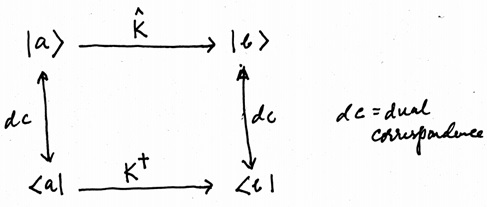
\includegraphics[width=100 mm]{adjoint.jpg}
\end{figure}

\paragraph{}
From Eqs. (\ref{eq:K}) and (\ref{eq:kdagger}) it follows that
\be
\langle c|b\rangle = \langle c|\hat{K}|a\rangle 
\ee
and
\be
\langle b|c\rangle = \langle a|\hat{K}^{\dag}|c\rangle .
\ee
Since $\langle b|c\rangle = \langle c|b\rangle^*$, we have
\be
\boxed{
\langle c|\hat{K}| a\rangle = \langle a |\hat{K}^{\dag}|c\rangle^*.
}
\label{eq:kdagger2}
\ee
Eq. (\ref{eq:kdagger2}) is the defining equation for the adjoint $\hat{K}^{\dag}$ of the operator $\hat{K}$.
In the scalar product notation (comma notation)
\[ \langle c|b\rangle \equiv (\psi_c, \psi_b) \]
Eq. (\ref{eq:kdagger2}) can be written as
\begin{eqnarray}
(\psi_c, \hat{K} \psi_a) &=& (\psi_a, \hat{K}^{\dag} \psi_c)^* \nonumber \\
&=& (\hat{K}^{\dag}\psi_c,\psi_a).
\end{eqnarray}
In particular, if we take $|c\rangle$ and $|a\rangle$ as the basis states $|i\rangle$ and $|j\rangle$, Eq. (\ref{eq:kdagger2}) 
becomes
\[ \langle i |\hat{K}|j\rangle = \langle j|\hat{K}^{\dag}|i\rangle^* \]
or,
\[ K_{ij}= \left(K^{\dag}\right)_{ji}^* \]
or,
\[ K^{\dag}_{ji}=K_{ij}^* \]
i.e.,
\[ K^{\dag}_{ij} = (K_{ji})^*.\]
In full matrix notation we can write
\be
[ \hat{K}^{\dag} ] = [ \hat{K} ]^{\dag},
\ee
where $[ \hat{K} ]$ is the matrix representation of the operator $\hat{K}$. Similarly for $\hat{K}^{\dag}$. Thus, the matrix representation
of the adjoint operator $\hat{K}^{\dagger}$ is the Hermitian conjugate of the matrix representation of $\hat{K}$.

\subsection{ Hermitian or self adjoint operator}
If $\hat{K}^{\dagger} = \hat{K}$, then $\hat{K}$ is said to be a self-adjoint or a Hermitian operator. The matrix representing
a Hermitian operaor is a Hermitian matrix i.e., 
\[ [K] =[K]^{\dag}\]
or,
\[ K_{ij}=K_{ji}^*.\]


\vspace{5 mm}
\noindent
{\bf Ex:}\newline
Show that $(\hat{A}\hat{B})^{\dag} = \hat{B}^{\dag}\hat{A}^{\dag}$.


\noindent {\bf Ans:}\newline
\be
\left(\psi_a,\hat{A}\hat{B}\psi_b\right) =\left((\hat{A}\hat{B})^{\dag}\psi_a,\psi_b\right).
\label{eq:AB1}
\ee
Also,
\be
\left(\psi_a,\hat{A}\hat{B}\psi_b\right)= \left( \hat{A}^{\dag}\psi_a,\hat{B}\psi_b\right)=
\left(\hat{B}^{\dag}\hat{A}^{\dag},\psi_b\right)
\label{eq:AB2}
\ee
Comparing Eqs. (\ref{eq:AB1}) and (\ref{eq:AB2}), we have
\be
\left( \hat{A}\hat{B}\right)^{\dag}=\hat{B}^{\dag}\hat{A}^{\dag}.
\ee


\subsection{Inverse operator}
An operator $\hat{B}$ is said to be the inverse of the operator $\hat{A}$ if
\be
\hat{A}\hat{B} = \hat{B}\hat{A}= \hat{I}.
\label{eq:inverse}
\ee
Obviously if $\hat{B}$ is the inverse of $\hat{A}$, then $\hat{A}$ is the inverse of $\hat{B}$. We write
\[ \hat{B} = \hat{A}^{-1}\]
or,
\[ \hat{A} = \hat{B}^{-1} \]
if Eq. (\ref{eq:inverse}) is satisfied.


\subsection{Unitary operator}
An operator $\hat{U}$ is said to be unitary if 
\be
\hat{U}\hat{U}^{\dag}=\hat{U}^{\dag}\hat{U} = \hat{I}
\ee
i.e., if
\be
\hat{U}^{\dag}=\hat{U}^{-1}.
\ee
Thus, for a unitary operator, its adjoint is also its inverse. 



\section{Functions of operators}
Consider a real-valued function $f(x)$ of a real variable $x$. Suppose that the function has a power series expansion 
\be
f(x) = f_0 + xf_1 + x^2 f_2 + \cdots.
\ee
If $\hat{A}$ is an operator, we can define the operator $\hat{f}(\hat{A})$ as
\be
\hat{f}(\hat{A}) = f_0 \hat{I} + \hat{A}f_1 + \hat{A}^2 f_2 + \cdots.
\ee
As an example of a function of an operator, consider the operator $e^{\lambda\hat{A}}$. This is defined as
\be
e^{\lambda\hat{A}}= \hat{I} + \lambda \hat{A} + \frac{\lambda^2}{2!} \hat{A}^2 + \frac{\lambda^3}{3!}\hat{A}^3 + \cdots.
\ee

\paragraph{}
One must be careful in manipulating functions of operators since operators do not commute with each other in general. For example,
if $\hat{A}\hat{B} \neq \hat{B}\hat{A}$, then
\be
e^{\hat{A}+\hat{B}} \neq e^{\hat{A}}e^{\hat{B}} \neq e^{\hat{B}}e^{\hat{A}}.
\ee
In the special case when $[\hat{A}, \hat{B}]$ is a number times the unit operator, i.e.,
\[ [\hat{A},\hat{B}] = c \hat{I} \]
where $c$ is a number (in general complex), then
\be
e^{\hat{A}+\hat{B}} = e^{\hat{A}}e^{\hat{B}}e^{-[\hat{A},\hat{B}]/2}.
\ee
This result is known as Weyl's identity. For example, in quantum mechanics we have
\[ [\hat{x},\hat{p}_x]=i\hbar \hat{I}. \]
So Weyl's identity would be satisfied by $\hat x$ and $\hat{p}_x$.


\vspace{5 mm}
\noindent {\bf Examples}

\noindent{\bf Ex}
Show that
\begin{equation}
e^{\lambda \hat{A}}\hat{B} e^{-\lambda \hat{A}} = \hat{B} + \lambda [\hat{A},\hat{B}] +\frac{\lambda^2}{2!}[\hat{A},[\hat{A},\hat{B}]]
+ \frac{\lambda^3}{3!}[\hat{A},[\hat{A},[\hat{A},\hat{B}]]]+ \cdots .
\end{equation}

\vspace{3 mm}
\noindent 
{\bf Ans:}\newline
Let
\[ f(\lambda)= e^{\lambda \hat{A}}\hat{B} e^{-\lambda \hat{A}}.\]
Therefore
\[
\frac{df(\lambda)}{d\lambda}= e^{\lambda \hat{A}}\hat{A}\hat{B} e^{-\lambda \hat{A}} - 
e^{\lambda \hat{A}}\hat{B}\hat{A} e^{-\lambda \hat{A}} = e^{\lambda \hat{A}}[\hat{A},\hat{B}] e^{-\lambda \hat{A}}.
\]
Differentiating one more time, we have
\[
\frac{d^2f(\lambda)}{d\lambda^2} = e^{\lambda \hat{A}}[\hat{A},[\hat{A},\hat{B}]] e^{-\lambda \hat{A}},
\]
and so on. Also
\[
f(0)=\hat{B},\;\; \left( \frac{df}{d\lambda}\right)_{\lambda = 0} =[\hat{A},\hat{B}], \;\;
\left(\frac{d^2f}{d\lambda^2}\right)_{\lambda =0} = [\hat{A},[\hat{A},\hat{B}]], \; \cdots 
\]
Expanding $f(\lambda)$ in a Taylor series:
\[
f(\lambda)=f(0) + \lambda \left( \frac{df}{d\lambda}\right)_{\lambda = 0} + 
\frac{\lambda^2}{2!} \left(\frac{d^2f}{d\lambda^2}\right)_{\lambda =0}+ \cdots
\]
we have
\[
e^{\lambda \hat{A}}\hat{B} e^{-\lambda \hat{A}} = \hat{B} + \lambda [\hat{A},\hat{B}] +\frac{\lambda^2}{2!}[\hat{A},[\hat{A},\hat{B}]]
+  \cdots .
\]


\section{Change of basis}
Supose we have a set of complete orthonormal basis set $\{|u_i\rangle\}$ in a Hilbert space. The orthonormality and completeness of the 
vasis set can be expressed as
\be
\langle u_i|u_j\rangle = \delta_{ij} \;\; {\text{orthonormality}}
\ee
and
\be 
\sum_i |u_i\rangle \langle u_i| = \hat{I}\;\; {\text{completeness}}.
\ee
In terms of the basis set $\{ |u_i\rangle \}$, an arbitrary ket $|\psi\rangle$ of the Hilbert space can be expanded as
\be
|\psi\rangle = \sum_i |u_i\rangle \langle u_i|\psi\rangle = \sum_i a_i |u_i\rangle,
\ee
where
\be
a_i= \langle u_1|\psi\rangle
\ee
is the component of $|\psi\rangle$ along $|u_i\rangle$. The numbers $a_i$ arranged as a column matrix is called the representation
of the ket $|\psi\rangle$ in the basis $\{ |u_i\rangle\}$.
Thus,
\be
|\psi\rangle \longrightarrow \begin{bmatrix} a_1\\a_2\\\vdots \end{bmatrix}
= \begin{bmatrix} \langle u_1|\psi\rangle \\\langle u_2|\psi\\\vdots \end{bmatrix}.
\ee
The conjugate of $|\psi\rangle$ in the dual space is written as the bra $\langle \psi|$. The matrix representation of 
$\langle \psi|$ is the row vector with components $\langle \psi|u_i\rangle$, i.e. $\langle u_i|\psi \rangle ^*$. Thus,
\be
\langle \psi| \longrightarrow \begin{bmatrix} \langle \psi|u_1\rangle & \langle \psi|u_2\rangle & \cdots \end{bmatrix}
= \begin{bmatrix} a_1^* & a_2^* & \cdots \end{bmatrix}.
\ee

\paragraph{}
Using the basis $\{ |u_i\rangle\}$, we can also write down the representation of an operator $\hat{A}$ as a square
matrix with elements $A_{ij}$ given by
\be
A_{ij}=\langle u_i|\hat{A}|u_j\rangle.
\ee
Writing in full 
\be
\hat{A} \rightarrow [A] = \begin{bmatrix}
A_{11} & A_{12} & A_{13} & \cdots \\
A_{21} & A_{22} & A_{23} & \cdots \\
A_{31} & A_{32} & A_{33} & \cdots \\
\vdots & \vdots & \vdots & \vdots
\end{bmatrix} 
\ee

\paragraph{}
Now, we make a change from the basis vectors $\{ |u_i\rangle, i=1,2,3, \cdots \}$ to a new set of orthonormal basis vectors
$\{ |u_i^{\prime}\rangle, i=1,2,3, \cdots \}$. The orthonormality and completeness of the new basis states can be expressed as
\be
 \langle u_i^{\prime}|u_i^{\prime}\rangle = \delta_{ij}
\ee
and
\be
\sum_i |u_i^{\prime}\rangle \langle u_i^{\prime}| = \hat{I}.
\ee
We can also write down the matrix representations of kets and operators in the new basis. We want to find how the components of the
ket $|\psi\rangle$ in the new basis relates to the components in the old basis. Similarly, we also want to know how the matrix
elements of an operator transform as we make the change of basis.


\subsection{Change of representation for kets}
Let $|\psi\rangle$ be an arbitrary ket in the vector space $V$. In the new basis $\{ |u_i^{\prime}\rangle \}$, the components
$a_i^{\prime}$ of the ket $|\psi\rangle$ are
\begin{eqnarray}
a_i^{\prime} &=& \langle u_i^{\prime}|\psi \rangle \nonumber \\
&=& \sum_j \langle u_i^{\prime}|u_j\rangle \langle u_j|\psi\rangle, 
\end{eqnarray}
or,
\be
a_i^{\prime} = \sum_j S_{ij}a_j
\label{eq:ket}
\ee
where we have defined
\be
S_{ij}= \langle u_i^{\prime}|u_j\rangle.
\ee
In matrix form Eq. (\ref{eq:ket}) is
\be
\begin{bmatrix} a_1^{\prime} \\ a_2^{\prime}\\ \vdots \end{bmatrix} =
\begin{bmatrix}
\langle u_1^{\prime}|u_1\rangle & \langle u_1^{\prime}|u_2\rangle & \hdots \\
\langle u_2^{\prime}|u_1\rangle & \langle u_2^{\prime}|u_2\rangle & \hdots \\
\vdots                          & \vdots                          & \vdots
\end{bmatrix}
\begin{bmatrix} a_1 \\ a_2 \\ \vdots \end{bmatrix}.
\ee
Before proceeding, we shall show that the matrix $[S] =(S_{ij})$ is unitary.

\subsubsection{To show that $[S]$ is unitary}

We start with the orthonormality of the new basis set, i.e., 
\[ \langle u_i^{\prime}|u_j^{\prime}\rangle = \delta_{ij} \]
or,
\[ \sum_k \langle u_i^{\prime}|u_k\rangle \langle u_k|u_j^{\prime}\rangle =\delta_{ij}, \]
or,
\[ \sum_k S_{ik}S_{jk}^* = \delta_{ij}, \]
or,
\[ \sum_{k} S_{ik}S^{\dag}_{kj} =\delta_{ij} \]
i.e.,
\[ [S][S]^{\dag} = [I].\]
Next, we use the orthonormality of the old basis set.
\[ \langle u_i|u_j\rangle = \delta_{ij} \]
or,
\[ \sum_k \langle u_i|u_k^{\prime}\rangle \langle u_k^{\prime}|u_j\rangle =\delta_{ij}, \]
or,
\[ \sum_k S^*_{ki}S_{kj} = \delta_{ij}, \]
or,
\[ \sum_{k} S^{\dag}_{ik}S_{kj} =\delta_{ij} \]
i.e.,
\[ [S]^{\dag}[S] = [I].\]
Thus, we have proved
\be
[S][S]^{\dag}= [S]^{\dag}[S] = [I],
\ee
i.e.,
$[S]$ is a unitary matrix.



\section{Transformation of the matrix elements of an operator due to a change of basis}
Next, we will discuss how the matrix elements of an operator transform if we make a change of basis. To do so, we proceed as follows.
\begin{eqnarray}
A^{\prime}_{ij} &=& \langle u_i^{\prime}|\hat{A}|u_j^{\prime}\rangle \nonumber \\
&=& \sum_{k,l} \langle u_i^{\prime}|u_k\rangle \langle u_k|\hat{A}|u_l\rangle \langle u_l|u_j^{\prime}\rangle \nonumber \\
&=& \sum_{k,l} \langle u_i^{\prime}|u_k\rangle A_{kl} \langle u_j^{\prime}|u_l\rangle^* \nonumber \\
&=& \sum_{k,l} S_{ik}A_{kl}S_{jl}^* .
\end{eqnarray} 
In the full matrix notation we can write
\be
[A]^{\prime} = [S][A][S]^{\dag} , 
\ee
or, since $[S]$ is unitary,
\be
[A]^{\prime} = [S][A][S]^{-1}.
\ee
Such a transformation of a square matrix is called a similarity transformation.









%
%\section{Adjoint operator}
%Consider the equation
%\begin{equation}\label{eqn:4.1}
%\ket{b} = \hat{K} \ket{a}
%\end{equation}
%The operator $\hat{K}$ carries the ket $\ket{a}$ to the ket $\ket{b}$. The dual of $\ket{a}$ and $\ket{b}$ are the bras $\bra{a}$ and $\bra{b}$ respectively. Then the operator which carries $\bra{a}$ to $\bra{b}$ is called the adjoint of $\hat{K}$ and is denoted by $\hat{K^\dagger}$. Thus in dual space \ref{eqn:4.1} is
%\begin{equation}\label{eqn:4.2}
%\bra{b} = \bra{a} \hat{K^\dagger}
%\end{equation}
%\begin{align}\label{eqn:4.3-4.4}
%	\text{ket space \ } \ket{a} _\rightarrow^{\hat{K}} \ket{b}\\
%	\text{bra space \ } \bra{a} _\rightarrow^{\hat{K^\dagger}} \bra{b}
%\end{align}
%Here bra space is the dual of ket space and
%\begin{align}\label{eqn:4.5-4.6}
%	\ket{a} _\rightarrow^{dc} \bra{a} \\
%	\ket{b} _\rightarrow^{dc} \bra{b}
%\end{align}
%dc $\equiv$ dual correspondence.\\
%
%From equation \ref{eqn:4.1} and \ref{eqn:4.2} it follows that
%\begin{equation}\label{eqn:4.7}
%\braket{c}{b} = \bra{c}\hat{K}\ket{a}
%\end{equation}
%and 
%\begin{equation}\label{eqn:4.8}
%\braket{b}{c} = \bra{a} \hat{K^\dagger} \ket{c}
%\end{equation}	 
%since
%\begin{equation}\label{eqn:4.9}
%\braket{b}{c} = \braket{c}{b}^*
%\end{equation}
%we have
%\begin{equation}\label{eqn:4.10}
%\bra{c} \hat{K} \ket{a} = \bra{a} \hat{K^\dagger} \ket{c}
%\end{equation}
%equation \ref{eqn:4.10} is the defining equation for the adjoint $\hat{K^\dagger}$ of the operator $\hat{K}$. In scalar product notation
%\begin{equation}\label{eqn:4.11}
%\braket{c}{b} \equiv \left(\psi_c, \psi_b \right)
%\end{equation}
%equation \ref{eqn:4.10} can be written as
%\begin{align}\label{eqn:4.12-4.13}
%	\left(\psi_c, \hat{K} \psi_a \right) 
%	&= \left(\psi_a, \hat{K^\dagger} \psi_c\right)^*\\
%	&=	\left(\hat{K^\dagger}\psi_c, \psi_a \right)
%\end{align}
%In particular, if we take $\ket{c}$ and $\ket{a}$ as the basis states $\ket{i}$ and $\ket{j}$, equation \ref{eqn:4.10} becomes
%\begin{align}\label{eqn:4.14-4.18}
%	\bra{i}\hat{K}\ket{j} &= \bra{j}\hat{K^\dagger}\ket{i}^* \\
%	K_{i j} &= \left(K^\dagger\right)_{j i}^* \\
%	K_{j i}^\dagger &= K_{i j}^* \\
%	K_{i j}^\dagger &= \left(K_{j i} \right)^* \\
%	\left[\hat{K^\dagger} \right] &= \left[K \right]^\dagger
%\end{align}
%i.e., The matrix representation of the adjoint operator is the hermitian conjugate of the matrix representation of $\hat{K}$.
%
%\section{Hermitian or Self-adjoint operator}
%If $\hat{K^\dagger} = \hat{K}$, then $\hat{K}$ is said to be a self-adjoint or a hermitian operator. For a hermitian operator
%\begin{equation}\label{eqn:4.19}
%\left[K\right] = \left[K^\dagger\right] = \left[K\right]^\dagger
%\end{equation}
%or
%\begin{equation}\label{eqn:4.20}
%K_{i j} = K_{j i}^*
%\end{equation}
%i.e., $\left[K\right]$ is a hermitian matrix.
%\begin{enumerate}[label=\textbf{Example \arabic*},start=1]
%	\item 
%	show that
%	\begin{equation}\label{eqn:4.21}
%	\left(A B\right)^\dagger = B^\dagger A^\dagger
%	\end{equation}
%	Answer: \\
%	\begin{equation}\label{eqn:4.22}
%	\left(\psi_a, \hat{A}\hat{B}\psi_b\right) = \left(\left(  \hat{A}\hat{B}\right)^\dagger\psi_a, \psi_b \right)
%	\end{equation}
%	Also
%	\begin{equation}\label{eqn:4.23}
%	\left(\psi_a, \hat{A}\hat{B}\psi_b\right) = \left(  \hat{A}^\dagger\psi_a, \hat{B}\psi_b \right) = \left(  \hat{B}^\dagger\hat{A}^\dagger\psi_a, \psi_b \right)
%	\end{equation}
%	Comparing these equation (equation \ref{eqn:4.22} and \ref{eqn:4.23}) we get,
%	\begin{equation}\label{eqn:4.24}
%	\left(\hat{A}\hat{B}\right)^\dagger = \hat{B}^\dagger \hat{A}^\dagger
%	\end{equation}
%\end{enumerate}
%\section{Inverse operator}
%An operator $\hat{B}$ is said to be the inverse of $\hat{A}$ if
%\begin{equation}\label{eqn:4.25}
%\hat{A}\hat{B} = \hat{B}\hat{A} = \hat{\mathbb{I}}
%\end{equation}
%Obviously, if $\hat{B}$ is the inverse of $\hat{A}$, then $\hat{A}$ is the inverse of $\hat{B}$. We write
%\begin{equation}\label{eqn:4.26}
%\hat{B} = \hat{A} ^{-1}
%\end{equation}
%or
%\begin{equation}\label{eqn:4.27}
%\hat{A} = \hat{B} ^{-1}
%\end{equation}
%If equation \ref{eqn:4.25} is satisfied.
%
%\section{Unitary operator}
%An operator $\hat{U}$ is said to be unitary if
%\begin{equation}
%\hat{U} \hat{U^\dagger} = \hat{U^\dagger} \hat{U} = \hat{\mathbb{I}}
%\end{equation}
%i.e., if
%\begin{equation}
%\hat{U^\dagger} = \hat{U}^{-1}
%\end{equation}
%Thus, for a unitary operator, its adjoint is $@@@@@@@@@@@@@@@@$
%
%\section{Function of Operators}
%

\chapter{sheet-5 : Eigenvalue and Eigenvectors of Operators}
%% writing by shahnoor
\ifpdf
\graphicspath{{Chapter5/figs/}}
\else
\graphicspath{{Chapter5/figs/}}
\fi


The ket $\ket{\alpha}$ is called the eigenvector or eigenket of the operator $A$ if
\begin{equation}
	A\ket{\alpha} = \alpha \ket{\alpha}
\end{equation}
The number $\alpha$ is called the eigenvalue. Thus the effect of $\hat{A}$ on an eigenket of $A$ is merely multiplication by a number.

\section{Eigenvalues and Eigenvectors of a Hermitian Operator}
We now take up the eigenvalue problem of a hermitian operators. Two theorems are of vital important in this content.
\begin{theorem}
	The eigenvalues of a hermitian operator are real.
\end{theorem}

\begin{theorem}
	The eigenvectors of a hermitian operator belonging to different eigenvalues are orthogonal.
\end{theorem}

\begin{proof}
	Let $A$ be a hermitian operator and 
	\begin{eqnarray}
		\label{chapter5.eqn1}
		A\ket{\alpha_1} &= \alpha_1 \ket{\alpha_1}\\
		\label{chapter5.eqn2}
		A\ket{\alpha_2} &= \alpha_2 \ket{\alpha_2}
	\end{eqnarray}
	From equation (\ref{chapter5.eqn1}) we have,
	\begin{equation}
		\bra{\alpha_2}A\ket{\alpha_1} = \alpha_1 \braket{\alpha_2}{\alpha_1}
		\label{chapter5.eqn3}
	\end{equation}
	Next we take the adjoint of equation (\ref{chapter5.eqn2})
	\begin{equation}
		\bra{\alpha_2}A^{\dagger} = \alpha_2^* \bra{\alpha_2}
	\end{equation}
	Since $A$ is hermitian, i.e., $A^\dagger = A$, we get
	\begin{equation}
		\bra{\alpha_2}A = \alpha_2^* \bra{\alpha_2}
	\end{equation}
	Hence
	\begin{equation}
		\bra{\alpha_2}A\ket{\alpha_1} = \alpha_2^* \braket{\alpha_2}{\alpha_1}
		\label{chapter5.eqn4}
	\end{equation}
	Combining equation (\ref{chapter5.eqn3}) and (\ref{chapter5.eqn4}) we get
	\begin{equation}
		(\alpha_1 - \alpha_2^*) \braket{\alpha_2}{\alpha_1} = 0
		\label{chapter5.eqn5}
	\end{equation}
	If we let $\alpha_2 = \alpha_1$ and recaling that $\braket{\alpha_1}{\alpha_1} \neq 0$, it follows that
	\begin{equation}
		\alpha_1 - \alpha_1^* = 0
	\end{equation}
	i.e., $\alpha_1$ is real. Since eigenvalues are proved to be real, we can write equation (\ref{chapter5.eqn5}) as
	\begin{equation}
		(\alpha_1 - \alpha_2) \braket{\alpha_2}{\alpha_1} = 0
		\label{chapter5.eqn6}
	\end{equation}
	If $\alpha_1 \neq \alpha_2$, we must have
	\begin{equation}
		\braket{\alpha_2}{\alpha_1} = 0
	\end{equation}
	i.e., eigenvectors belongings to differnt eigenvalues are orthogonal. Owing to the linearity of the operators $\hat{A}$ we can normalize the eigenvectors. We shall therefore usually assume that 
	\begin{equation}
		\braket{\alpha_1}{\alpha_2} = \delta_{\alpha_1\alpha_2}
	\end{equation}
	Thus, the eigenvectors of a hermitian operator form an orthonormal (and hence linearly independent vectors), i.e.,
	\begin{equation}
		\braket{\alpha_i}{\alpha_j} = \delta_{\alpha_i\alpha_j}
	\end{equation}
\end{proof}


\section{Determination of eigenvalues and eigenvectors of a Hermitian Operator}
	Let $A$ be a hermitian operator. Consider the eigenvalue equation
	\begin{equation}
		A \ket{\lambda} = \lambda \ket{\lambda}
		\label{chapter5.eqn7-eigenvalue-hermitian}
	\end{equation}
	To find the eigenvalue and the corresponding eigenvectors, we have to choose a basis in the vector space and convert the operator equation (\ref{chapter5.eqn7-eigenvalue-hermitian}) into a matrix equation. For simplicity, we will assume that the vector space is finite dimensional with dimension $n$. \\
	Now choosing an orthonormal basis set $\{\ket{u_i}\}$, we can cast equation (\ref{chapter5.eqn7-eigenvalue-hermitian}) as a matrix equation of the following form:
	\begin{equation}
		\left[
		\begin{matrix}
			A_{11} & A_{12} & \ldots & A_{1n} \\
			A_{21} & A_{22} & \ldots & A_{2n} \\
			\vdots & \vdots & \vdots \vdots \vdots & \vdots \\
			A_{n1} & A_{n2} & \ldots & A_{nn} \\
		\end{matrix}
		\right]\left[
		\begin{matrix}
			x_1 \\ x_2 \\ \vdots \\ x_n
		\end{matrix}
		\right]
		=
		\lambda
		\left[
		\begin{matrix}
			x_1 \\ x_2 \\ \vdots \\ x_n
		\end{matrix}
		\right]
		\label{chapter5.eqn7-eigenvalue-matrix-form}
	\end{equation}
	Here $x_1, x_2, \ldots, x_n$ are the components of the eigenvector $\ket{\lambda}$ in \textbf{directions} $\ket{u_1}, \ket{u_2}, \ldots, \ket{u_n}$ respectively, i.e.,
	\begin{equation}
		x_i \equiv \braket{u_i}{\lambda} \text{ ; } i=1,2,\ldots,n
	\end{equation}
	Equation (\ref{chapter5.eqn7-eigenvalue-matrix-form} is a set of linear homogeneous equations which possess non-trivial solutions only if)

\begin{equation}
	\left|
	\begin{matrix}
		(A_{11}-\lambda) & A_{12} & \ldots & A_{1n} \\
		A_{21} & (A_{22}-\lambda) & \ldots & A_{2n} \\
		\vdots & \vdots & \vdots \vdots \vdots & \vdots \\
		A_{n1} & A_{n2} & \ldots & (A_{nn}-\lambda) \\
	\end{matrix}
	\right| = 0
\end{equation}
	or in short
	\begin{equation}
		\det(A_{ij} - \lambda \delta_{ij}) = 0
	\end{equation}
	In matrix notation, we can write
	\begin{equation}
		\left|\mathbb{A} - \lambda \mathbb{1} \right| = 0
	\end{equation}
	This equation, which is a polynomial equation of degree $n$ in the unknown $\lambda$, is called the secular equation of the matrix $\mathbb{A}$. Solving this equation we get $n$ roots which we label as 
	\begin{equation}
		\lambda_1, \lambda_2, \ldots, \lambda_n \nonumber
	\end{equation}
	Now, we can distinguish two cases. If the $n$ eigenvalues are all distinct, we say that the eigenvalues are \textit{non-degenerate}. However, it may so happen that some of the eigenvalues are repeated. Those eigenvalues which are repeated are called \textit{degenerate}
	eigenvalues and the number of times an eigenvalue is repeated is called the \textit{order of degeneracy} of that eigenvalue.
	
	\section{Non-degenerate roots}
	In this case all the roots $\lambda_i$ are distinct and there are $n$ of them if the vector space is $n$ dimensional. If $A$ is hermitian, the roots are real. For a non-hermitian operator some or all of the roots may be complex.
	
	
	Now, for each eigenvalue (root of secular equation) we can solve the eigenvalue equation (\ref{chapter5.eqn7-eigenvalue-matrix-form}) to get $n$ linearly independent eigenvectors $\ket{\lambda_i}$. Since the $\ket{\lambda_i}$'s are linearly independent, they span the $n$ dimensional vector space, i.e., they form a complete set of basis vectors.
	
	
	
	If $A$ is hermitian, the eigenvectors are guarenteed to b orthogonal, i.e., $\braket{\lambda_i}{\lambda_j} = 0$ if $i\neq j$. However, for a non-hermitian operator the eigenvectors may or may not be orthogonal.
	Using the eigenvectors of $A$ as the basis (This basis is called the eigenbasis of $A$), the matrix representation of $A$ is
	\begin{equation}
		A_{ij}^\prime \equiv \bra{\lambda_i} A \ket{\lambda_j} = \lambda_j \braket{\lambda_i}{\lambda_j}
		\label{chapter5.eqn8-matrix-reps}
	\end{equation}
	For hermitian $A$, we always have $\braket{\lambda_i}{\lambda_j} = 0$ if $i \neq j$, and , further we can normalize each eigenvector $\ket{\lambda_i}$. Thus, for a hermitian operator, the eigenbasis is an orthogonal set, i.e., 
	\begin{equation}
		\braket{\lambda_i}{\lambda_j} = \delta_{ij}
		\label{chapter5.eqn9-eigenbasis}
	\end{equation}
	Therefore, the matrix representation of the oprator $A$ in its eigenbasis is diagonal, i.e.,
	\begin{equation}
		A_{ij}^\prime = \lambda_j\delta_{ij}
		\label{chapter5.eqn9-matrix-reps-diagonal}
	\end{equation}
	Writing out the matrix ($A_{ij}^\prime$) in full
	\begin{equation}
		\mathbb{A}^\prime = \left[
		\begin{matrix}
			\lambda_1 &	0	& 0	& \ldots	& 0 \\			
			0 &	\lambda_2	& 0	& \ldots	& 0 \\
			\vdots &	\vdots	& \vdots	& \vdots \quad \vdots	& \vdots \\	
			0 & 0	& 	 0 & \ldots	& \lambda_n  \\
		\end{matrix}
		\right]
	\end{equation}
	An operator or a matrix $\mathbb{A}$ is said to be diagonalizable, if we can find a basis in which the matrix becomes diagonal. For a hermitian operator we can always find a basis, the eigenbasis of the operator, in which the matrix representation of the operator is diagonal with the eigenvalues as the diagonal elements.
	
	
	
	For a non-hermitian operator in an $n$  dimensional vector space, there is no guarantee that the matrix reprsentation $A_{ij}^\prime$ in the eigenbasis of the operator is diagonal. This is because, in general, the eigenvectors are  not orthogonal, i.e., $\braket{\lambda_i}{\lambda_j} \neq \delta_{ij}$
	
	\section{Degenerate roots}
	The secular equation (\ref{chapter5.eqn8-matrix-reps}) may have roots some or all of which are repeated. So, the number of \underline{distinct} eigenvalues is now less than the dimension of the vector space.
	
	
	As an example, suppose we have a six-dimensional vector space ($n=6$) with three distinct roots $\lambda_1, \lambda_2, \lambda_3$. Suppose $\lambda_1$ is repeated three times, $\lambda_2$ is repeated two times and $\lambda_3$ occurs only once. Thus the six roots of the secular equation are $\lambda_1, \lambda_1, \lambda_1, \lambda_2, \lambda_2, \lambda_3$.
	
	
	
	
	
	We say $\lambda_1$ is three-fold degenerate, $\lambda_2$ is two-fold degenerate and $\lambda_3$ is non-degenerate. We represent the order of degeneracy of a distinct eigenvalue $\lambda_i$ by $g_{\lambda_i}$. In the present example, $g_{\lambda_1}=3, g_{\lambda_2}=2$ and $ g_{\lambda_3}=1$. We have
	\begin{equation}
		g_{\lambda_1} + g_{\lambda_2} + g_{\lambda_3} = 6 \quad \text{dimension of the vector space}
	\end{equation}
	Now, it may be shown that, for a \underline{hermitian operator} if a root $\lambda$ is $g$-fold degenerate, there are always $g$ linearly independent eigenvectors corresponding to $\lambda$. For a non-hermitian operator, there may not exist as many linearly independent eigenvectors as the order of degeneracy.
	
	
	
	In the above example, if $\lambda_1, \lambda_2$ and $\lambda_3$ are eigenvalues of a hermitian operator, there are three linearly independent eigenvectors with eigenvalue $\lambda_1$, two linearly independent eigenvectors with eigenvalue $\lambda_2$ and one eigenvector with eigenvalue $\lambda_3$. Thus, the total number of linearly indepent eigenvector is six, the same as the dimension of the vector space. Hence these six linearly independent eigenvectors form a \textit{complete basis set of vectors}.
	
	
	
	If, however, $\lambda_1, \lambda_2$ and $\lambda_3$ are eigenvalues of a non-hermitian operator with the same eigenvalues, there may not exist three linearly independent eigenvectors with eigenvalue $\lambda_1$, or  two linearly independent eigenvectors with eigenvalue $\lambda_2$. In such a situation, the number of linearly independent eigenvectors of the non-hermitian operator $A$ is less than the dimension $n$ of the vector space. Hence, these eigenvectors \textit{do not form a basis set} for a $n$ dimensional vector space.
	
	
	
	\section{Digonalization of a Hermitian Operator}
	Let $A$ be a hermitian operator with distinct eigenvalues $\lambda_1,\lambda_2\ldots$. Some or all of the eigenvalues may be degenerate, with the order or degree of degeneracy of an eigenvalue $\lambda_i$ being denoted by $g_{\lambda_i}$. If $g_{\lambda_j}=1$ for some $\lambda_j$, then $\lambda_j$ is said to be non-degenerate.
	
	
	Since $A$ is hermitian there will always be $g_{\lambda_i}$ linearly independent eigenvectors, each belonging to the same eigenvalue $\lambda_i$. We will now require another index, $s^{(i)}$, to distinguish between these linearly independent eigenvectors. We write
	\begin{equation}
		A \ket{\lambda_i, s^{(i)}} = \lambda_i \ket{\lambda_i, s^{(i)}}
		\label{chapter5.eqn9-eigenvectors-with-two-index}
	\end{equation}
	where $s^{(i)} = 1, 2, \ldots, g_{\lambda_i}$. A linear combination of the degenerate eigenvectors is also an eigenvector with the same eigenvalue $\lambda_i$. So we have
	\begin{equation}
		A \left(\sum_{s^{(i)}}^{g_{\lambda_i}}  C_{s^{(i)}} \ket{\lambda_i, s^{(i)}}\right) = \lambda_i \left(\sum_{s^{(i)}}^{g_{\lambda_i}}  C_{s^{(i)}} \ket{\lambda_i, s^{(i)}}\right)
		\label{chapter5.eqn10-combination-degenerate-eigenvectors}
	\end{equation}
	Thus, the set of vectors $\{ \ket{\lambda_i, s^{(i)}}; \quad \lambda_i \quad \text{fixed}, \quad s^{(i)}=1,2\ldots,g_{\lambda_i} \}$ spans a subspace, called the eigen subspace of $\lambda_i$, of the original $n$ dimensional vector space. The eigenvectors belonging to a degenerate eigenvalue need not be orthogonal to each other even if they are linearly independent, as the general theorem of hermitian operators proves the orthogonality of eigenvectors belonging to different eigenvalues.
	
	
	
	However, using Schmidt orthonormalization procedure (see section (\ref{chapter2.schmidt-orthonormalization-method})), we can get a set of $g_{\lambda_i}$ orthogonal 
	eigenfunctions %@@@@@@@ or
%	 eigenvectors %@@@@@@@ ?
	  of eigenvalue $\lambda_i$ from a set of $g_{\lambda_i}$ linearly independent set of
	  eigenfunctions
%	 eigenvectors %@@@@@@@ ?
	   of eigenvalue $\lambda_i$.
	   
	   
	   Thus, all the eigenvectors of the hermitian operator, wherether belonging to same or different eigenvalues can be considered as orthogonal to each other. Further, they are also normalized. Using the set of orthonormal eigenfunctions as the basis, the matrix representation of $A$ is diagonal.
	   
	   
	   
	   As a concrete example of diagonalization of a hermitian operator, suppose we have a finite seven-dimensional linear vector space. If, all the eigenvectors are non-degenerate, then there are seven distinct eigenvalues $\lambda_1, \ldots, \lambda_7$ and corresponding to each eigenvalue there will be one eigenvector $\ket{\lambda_1}, \ldots, \ket{\lambda_7}$. These eigenvectors are orthogonal and they are normalized. Using the eigenvectors as the basis, the matrix representation of $A$ is 
	   \begin{equation}
		   A = \left[
		   \begin{matrix}
	\lambda_1 & 0 & 0 & 0 & 0 & 0 & 0 \\
	0 & \lambda_2 & 0 & 0 & 0 & 0 & 0 \\
	0 & 0 & \lambda_3 & 0 & 0 & 0 & 0 \\
	0 & 0 & 0 & \lambda_4 & 0 & 0 & 0 \\
	0 & 0 & 0 & 0 & \lambda_5 & 0 & 0 \\
	0 & 0 & 0 & 0 & 0 & \lambda_6 & 0 \\
	0 & 0 & 0 & 0 & 0 & 0 & \lambda_7 \\
		   \end{matrix}
		   \right]
	   \end{equation}
	But if some of the eigenvalues are degenerate, then the number of distinct eigenvalues will be less than seven. Suppose that there are three distinct eigenvalues $\lambda_1, \lambda_2, \lambda_3$. Also suppose that $\lambda_1$ is three-fold degenerate and $\lambda_2$ and $\lambda_3$ both are two-fold degenerate. Thus $g_{\lambda_1}=3, g_{\lambda_2}=2, g_{\lambda_3}=2$ and $g_{\lambda_1} + g_{\lambda_2} + g_{\lambda_3}=7$ which is the dimension of the vector space.
	
	
	
	There are three linearly independent (but not necessarily orthogonal) eigenvectors with eigenvalue $\lambda_1$ and two linearly independent eigenvectors for each eigenvalue $\lambda_2$ and $\lambda_3$. The eigenvectors with eigenvalue $\lambda_1$ can be labled as 
	$\ket{\lambda_1, s^{(1)}}$ with $s^{(1)} = 1,2,3$, i.e., $\ket{\lambda_1,1}, \ket{\lambda_1,2}, \ket{\lambda_1,3}$.
	
	These three eigenvectors span a subspace of the original seven-dimensional vector space $H$. The subspace is called the eigensubspace of $\lambda_1$ and is denoted by $H_{\lambda_1}$ or simply $H_1$. The eigenvectors belonging to $\lambda_2$ and $\lambda_3$ are labeled similarly. Then two linearly independent eigenvectors with eigenvalue $\lambda_2$ span a two-dimensional subspace $H_2$ and the two linearly independent vectors belonging to $\lambda_3$ span the eigensubspace $H_3$. These three subspaces make up the full vector space $H$. We write
	\begin{equation}
		H = H_1 \bigoplus H_2 \bigoplus H_3
	\end{equation}
	The seven linearly independent eigenvectors $\{\ket{\lambda_i, s^{(i)}}, \quad s^{(i)}=1,2,\ldots g_{\lambda_i}, \quad i=1,2,3 \}$
	can now be used as a basis to find the matrix representation of $A$. If the basis vectors within an eigensubspace are not made orthogonal, the matrix representation of $A$ is block-diagonal as shown below.
	\begin{equation}
		\left[\begin{array}{@{}c|c@{}|c@{}}
		\begin{matrix}
		a_{11} & a_{12} & a_{13} \\
		a_{21} & a_{22} & a_{23} \\
		a_{31} & a_{32} & a_{33}
		\end{matrix}
		& \bigzero & \bigzero\\
		\hline
		\bigzero &
		\begin{matrix}
		b_{11} & b_{12} \\
		b_{21} & b_{22}
		\end{matrix}
		& \bigzero \\
		\hline
		\bigzero & \bigzero &
		\begin{matrix}
		c_{11} & c_{12} \\
		c_{21} & c_{22}
		\end{matrix}
		\end{array}\right]
	\end{equation}
	
%	\[
%	\begin{array}{l@{{}={}}c}
%	\text{Mat}_{\varphi\text{ to }M} & \left(\begin{array}{@{}ccccc@{}}
%	1 & 1 & 1 & 1 & 1 \\
%	0 & 1 & 0 & 0 & 1 \\
%	0 & 0 & 1 & 0 & 1 \\
%	0 & 0 & 0 & 1 & 1 \\
%	0 & 0 & 0 & 0 & 1
%	\end{array}\right)
%	\end{array}
%	\]
%	
%
%	\[
%	\text{Mat}_{\varphi\text{ to }M} = \kbordermatrix{
%		& c_1 & c_2 & c_3 & c_4 & c_5 \\
%		r_1 & 1 & 1 & 1 & 1 & 1 \\
%		r_2 & 0 & 1 & 0 & 0 & 1 \\
%		r_3 & 0 & 0 & 1 & 0 & 1 \\
%		r_4 & 0 & 0 & 0 & 1 & 1 \\
%		r_5 & 0 & 0 & 0 & 0 & 1
%	}
%	\]
	
	Writing with basis
	\begin{equation}
	\begin{blockarray}{cccccccc}
	\ & 1 & 2 & 3 & 4 & 5 & 6 & 7 \\
	\ & \ket{\lambda_1, 1} & \ket{\lambda_1, 2} & \ket{\lambda_1, 3} & \ket{\lambda_2, 1} & \ket{\lambda_2, 2} & \ket{\lambda_3, 1} & \ket{\lambda_3, 2} \\
		\begin{block}{c[ccccccc]}
		\bra{\lambda_1, 1} & a_{11} & a_{12} & a_{13} & 0 & 0 & 0 & 0 \\
		\bra{\lambda_1, 2} & a_{21} & a_{22} & a_{23} & 0 & 0 & 0 & 0 \\
		\bra{\lambda_1, 3} & a_{31} & a_{32} & a_{33} & 0 & 0 & 0 & 0 \\ 
		\bra{\lambda_2, 1} & 0 & 0 & 0 & b_{11} & b_{12} & 0 & 0 \\
		\bra{\lambda_2, 2} & 0 & 0 & 0 & b_{21} & b_{22} & 0 & 0 \\ 
		\bra{\lambda_3, 1} & 0 & 0 & 0 & 0 & 0 & c_{21} & c_{22}\\
		\bra{\lambda_3, 2} & 0 & 0 & 0 & 0 & 0 & c_{21} & c_{22}  \\ 
		\end{block}
	\end{blockarray}
	\end{equation}
	Each non-zero block is a square matrix. The first block is a $3\times 3$ matrix, the second one is a $2\times 2$ matrix and the rhird one is a $2\times 2$ matrix. These blocks themselves are not diagonal if the basis vectors of the three eigensubspaces are not orthogonalized. If we orthogonalize the basis vector in each eigensubspace, then each block will also be diagonal. The matrix representation of $A$ will then be
	
	\begin{equation}
	\begin{blockarray}{cccccccc}
	\ & \ket{\lambda_1, 1} & \ket{\lambda_1, 2} & \ket{\lambda_1, 3} & \ket{\lambda_2, 1} & \ket{\lambda_2, 2} & \ket{\lambda_3, 1} & \ket{\lambda_3, 2} \\
	\begin{block}{c[ccccccc]}
	\bra{\lambda_1, 1} & \lambda_1 & 0 & 0 & 0 & 0 & 0 & 0 \\
	\bra{\lambda_1, 2} & 0 & \lambda_1 & 0 & 0 & 0 & 0 & 0 \\
	\bra{\lambda_1, 3} & 0 & 0 & \lambda_1 & 0 & 0 & 0 & 0 \\ 
	\bra{\lambda_2, 1} & 0 & 0 & 0 & \lambda_2 & 0 & 0 & 0 \\
	\bra{\lambda_2, 2} & 0 & 0 & 0 & 0 & \lambda_2 & 0 & 0 \\ 
	\bra{\lambda_3, 1} & 0 & 0 & 0 & 0 & 0 & \lambda_3 & 0\\
	\bra{\lambda_3, 2} & 0 & 0 & 0 & 0 & 0 & 0 & \lambda_3  \\ 
	\end{block}
	\end{blockarray}
	\end{equation}
	Thus the matrix representation of a hermitian operator $A$ is diagonalized.
	
	
	We have proved that a hermitian operator (or a hermitian matrix) is always diagonalizable in a finite dimensional vector space. By diagonalizable we mean that we can always find a basis in which the matrix representation of $A$ is diagonal. This basis is simply the basis consisting of the orthogonalized eigenvectors of $A$, called eigenbasis of $A$.
	
	
	 The eigenvectors of a non-hermitian operator my be fewer in numbers than the dimension of the vector space if there is degeneracy. If an  eigenvector $\lambda_i$ is $g_i$-fold degenerate, then the number of linearly independent eigenvectors belonging to $\lambda_i$ may be less than $g_i$. Therefore, the eigenvectors of a non-hermitian operator cannot form a basis set for the vector space. Therefore, a non-hermitian operator is not diagonalizable.
	
	
	\section{Basis independence of the eigenvalues of an Operator}
	Basis independence refers to representation independence. To find the eigenvalues of a hermitian operator $\hat{A}$, first we choose an orthonormal basis set $\{\ket{u_i}\}$ and form the matrix representation of the operator. Then we solve the secular equation to find the eigenvalues. Although we have to integrate a basis set to find the eigenvalues, it is easy to verify that the eigenvalues are independent of the choice of the basis. 
	
	
	Indeed, if we choose a new orthogonal set of basis vectors $\{\ket{u_i}\}$ which are related to the old set according to 
	\begin{equation}
		\ket{u_i^\prime} = \sum_j \ket{u_j}\braket{u_j}{u_i^\prime}
	\end{equation}
	Then the new matrix representation of the operator $A$ is related to the old representation by a similarigy transformation with a \textit{unitary} matrix. This is easy to see
	\begin{eqnarray}
		A_{ij}^\prime 
		&\equiv \bra{u_i\prime} A \ket{u_j^\prime} \nonumber\\
		&= \sum_{jk} \braket{u_i^\prime}{u_j}\bra{u_j}A\ket{u_k}\braket{u_k}{u_j^\prime} \nonumber\\
		&= \sum_{jk} S_{ij} A_{jk} S_{jk}^* \nonumber\\
		&= \sum_{jk} S_{ij} A_{jk} S_{jk}^\dagger
		\label{chapter5.eqn2-similarity-trans}
	\end{eqnarray}
	Where we have defined the matrix $S$ as
	\begin{equation}
		S_{ij} \equiv \braket{u_i^\prime}{u_j}
	\end{equation}
	The matrix $S$ is unitary as shown precisely. In matrix notation, we write equation (\ref{chapter5.eqn2-similarity-trans}) as,
	\begin{equation}
		A^\prime = S A S^\dagger = S A S^{-1}
	\end{equation}
	since $S$ is unitary matrix. Then
	\begin{eqnarray}
		\det(\mathbb{A}^\prime - \lambda \mathbb{I}) 
		&= \det(\mathbb{S}\mathbb{A}^\prime \mathbb{S}^{-1} - \lambda \mathbb{S} \mathbb{I} \mathbb{S}^{-1}) \nonumber \\
		&= \det(\mathbb{S}(\mathbb{A} - \lambda \mathbb{I}) \mathbb{S}^{-1})\nonumber \\
		&= \det(\mathbb{A} - \lambda \mathbb{I})
	\end{eqnarray}
	Thus, there is no change in the secular equation even if we change the basis set. Since the eigenvalues are the roots of the secular equation, the eigenvalues are representation independent. They are characteristics of the operator $\hat{A}$ itself, and not of any particular representation.
	
	

	Next, we will show that the determinant and the trace of the matrix representation $A$ are independent of the basis used for the representation.
	
	Since $\mathbb{A}^\prime = \mathbb{S} \mathbb{A} \mathbb{S}^{-1}$ we have 
	\begin{eqnarray}
		\det(\mathbb{A}^\prime) 
		&= \det(\mathbb{S} \mathbb{A} \mathbb{S}^{-1}) \nonumber \\
		&= \det(\mathbb{S}^{-1}\mathbb{S} \mathbb{A} ) \nonumber \\
		&= \det(\mathbb{A})
	\end{eqnarray}
	i.e., the determinant is independent of the representation.
	
	We also have
	\begin{equation}
		\Tr (\mathbb{A}^\prime) = \Tr (\mathbb{S}\mathbb{A}^\prime\mathbb{S}^{-1})=\Tr(\mathbb{S}^{-1}\mathbb{S} \mathbb{A}) = \Tr (\mathbb{A})
	\end{equation}
	i.e., the trace is also independent of the representation. In the above derivations, we have used the identities,
	\begin{eqnarray}
		\det( \mathbb{A}\mathbb{B}) = \det(\mathbb{B}\mathbb{A}) \\
		\Tr( \mathbb{A}\mathbb{B}) = \Tr(\mathbb{B}\mathbb{A})
	\end{eqnarray}
	where $\mathbb{A}$ and $\mathbb{B}$ are square matrices. Now, if we use the eigenbasis of the hermitian operator $A$ for the representation, then $\mathbb{A}$ is a diagonal matrix with
	\begin{eqnarray}
		\det \mathbb{A} &= \prod_i \lambda_i \\
		\Tr \mathbb{A} &= \sum_i \lambda_i 
	\end{eqnarray}
	If an eigenvalue is $g$-fold degenerate, then that eigenvalue has to be repeated $g$ times while calculating the determinant and trace of the matrix $\mathbb{A}$.
	
	
	
	\section{Infinite dimensional vector space}
	We have shown that a linear operaor is a finite $n$-dimensional vector space has $n$ eigenvalues some of which may be repeated. If the operator is hermitian, then the eigenvalues are real and eigenvectors belonging to different eigenvalues are orthogonal and hence linearly independent.
	
	Further, if an eigenvalue $\lambda$ of a hermitian operator is $g$-fold degenerate, then there are $g$ linearly independent eigenvectors corresponding to $\lambda$, these degenerate eigenvectors are not necessarily orthogonal even if they are linearly independent. However, we can orthogonalize the degenerate eigenvectors using the Schmidt orthonormalization procedure (see section (\ref{chapter2.schmidt-orthonormalization-method})). 
	
	
	Thus in a finite $n$-dimensional vector space, the eigenvectors of any hermitian operator form a set of orthonormal basis vectors.
	
	
	In an infinite dimensional vector space, the number of eigenvalues and eigenvectors of a hermitian operators are infinitely many. However, it is possible that the eigenvectors of some hermitian operators do not form a complete set in an infinite dimensional vector space.

	
	Hermitian operators are of vital importance in quantum mechanics because to every observable (e.g., position, linear momentum, angular momentum, spin etc.) we \textit{associate} a corresponding hermitian operator. Of course, there are hermitian operators which are not associated with any observable.
	
	
	The eigenvectors of a hermitian operator representing a physical observable form a complete set even in an infinite-dimensional Hilbert space. The eigenvectors of a hermitian operator not associated with any observale may not form a complete basis set in an infinite dimensional space.
	
	
	
	\section{Completeness condition for the eigenvectors of a Hermitian Operator}
	Let us assume that the eigenvalue spectrum of a hermitian operator $\hat{A}$ form a discrete set. In other words, the eigenvalues $a_i,\quad i=1,2,\ldots$ of the operator are discrete real numbers.
	
	Assume, for the time being, that the eigenvalues are non-degenerate so that these is only one linearly independent eigenvectors $\ket{a_i}$ corresponding to each eigenvalue $a_i$. The eigenvectors $\{\ket{a_i}, i=1,2,\ldots\}$ form a complete orthogonal set of basis vectors. Therefore, an arbitrary vector $\ket{\psi}$ of the vector space can be expanded as a linear combination of the vector in the basis set, i.e.,
	\begin{equation}
		\ket{\psi} = \sum_{i} a_i \ket{a_i}
	\end{equation}
	where $c_i = \braket{a_i}{\psi}$. Therefore, we can write
	\begin{equation}
		\ket{\psi} = \sum_i \braket{a_i}{\psi} \ket{a_i} = \sum_i \ket{a_i}\braket{a_i}{\psi}
	\end{equation}
	Since $\ket{\psi}$ is arbitrary, we must have
	\begin{equation}
		\hat{\mathbb{1}} = \sum_i \ket{a_i}\bra{a_i} = \sum_i \hat{P}_i
		\label{chapter5.eqn1-completeness}
	\end{equation}
	where
	\begin{equation}
		\hat{P}_i = \ket{a_i}\bra{a_i}
		\label{chapter5.eqn2-projection}
	\end{equation}
	is the projection along $\ket{a_i}$.
	
	Using the basis $\{\ket{u_i}\}$, any operator $\hat{O}$ can be expressed as 
	\begin{eqnarray}
		\hat{O} = \hat{\mathbb{1}} \hat{O} \hat{\mathbb{1}} 
		&= \sum_{i,j} \ket{a_i}\bra{a_i} \hat{O} \ket{a_j}\bra{a_j} \nonumber \\
		&= \sum_{i,j} \ket{a_i} O_{ij} \bra{a_j}
		\label{chapter5.eqn3-operator-as-matrix}
	\end{eqnarray}
	where $O_{ij} \equiv \bra{a_i} \hat{O} \ket{a_j}$ are the matrix element of  $\hat{O}$ in the basis $\{\ket{u_i}\}$. Since basis is the eigenbasis of the operator $\hat{A}$, the matrix elements of $\hat{A}$ in the basis will be diagonal, i.e., 
	\begin{equation}
		\hat{A} = \sum_i a_i \ket{a_i}\bra{a_i} = \sum_i a_i \hat{P}_i
		\label{chapter5.eqn4-diagonalized-operator-projection}
	\end{equation}
	Any other oberator $\hat{B}$ will in general not be diagonal in the eigenbasis of $\hat{A}$ unless the eigenvectors of $\hat{B}$ and $\hat{A}$ coincide. Later, we will see that two operators $\hat{A}$ and $\hat{B}$ have simultaneous eigenvectors if they commute, i.e., if $[\hat{A},\hat{B}]=0$.
	
	
	Now, we will generalize the notation to include degeneracy, suppose the eigenvalue $a_i$ is a $g_i$ fold degenerate. Then the eigenvectors belonging to the eigenvalue $a_i$ is written as $\ket{a_i, s^{(i)}}$ where $s^{(i)}$ can take values $1,2,\ldots, g_i$. The set of vectors $\{\ket{a_i, s^{(i)}}, \quad s^{(i)}=1,2,\ldots,g_i;\quad i=1,2,\ldots\}$ Form a complete orthogonal set. The completeness condition is
	\begin{equation}
		\sum_{i=1}^{\infty} \sum_{s^{i}=1}^{g_i} \ket{a_i, s^{(i)}}\bra{a_i, s^{(i)}} = \hat{\mathbb{1}}
		\label{chapter5.eqn5-completeness-degenerate}
	\end{equation}
	and the orthogonality condition is
	\begin{equation}
		\braket{a_i, s^{(i)}}{a_j, s^{(j)}} = \delta_{ij}\delta_{s^{i}s^{(j)}}
		\label{chapter5.eqn6-orthogonality-degenerate}
	\end{equation}
	We can rewrite equation (\ref{chapter5.eqn5-completeness-degenerate}) as (exactly as the non degenerate case)
	\begin{equation}
		\hat{\mathbb{1}} = \sum_i \hat{P}_i
		\label{chapter5.eqn7-completeness-degenerate-rewrite}
	\end{equation}
	where
	\begin{equation}
		\hat{P}_i = \sum_{s^{(i)}=1}^{g_i} \ket{a_i, s^{(i)}}\bra{a_j, s^{(j)}}
		\label{chapter5.eqn8-projection-degenerate}
	\end{equation}
	is the projection operator on the eigensubspace of $a_i$. The operator $\hat{A}$ can then be written in its own eigenbasis as 
	$\hat{A} = \sum_i a_i \hat{P}_i$ with $\hat{P}_i$ given in equation (\ref{chapter5.eqn8-projection-degenerate})
	
	
	
	\section{Hermitian operator with continuous eigenvalue spectrum}
	In Quantum Mechanics we encounter hermitian operator like position operator, momentum operator whose eigenvalues range over a continuum of real values. Such an eigenvalue spectrum is called continuous. There are also hermitian operators whose eigenvalue spectrum may be both discrete and continuous.
	
		\subsection{Continuous Spectrum}
		Let us consider an operator $A$ whose eigenvalues can vary continuously over a certain domain of real numbers
		\begin{equation}
			A \ket{a} = a \ket{a}
			\label{chapter5.eqn9-eigenvalue}
		\end{equation}
		If there is degeneracy, we will put in a second index $s$ to distinguish between degenerate vectors. Thus we may write $\ket{a\quad s}$ to denote a degenerate eigenvector. We assume that there is no degeneracy. In case of degeneracy it is a simple matter to generalize our notations. We assume that the vectors $\ket{a}$ form a complete set. The completeness condition can be written as
		\begin{equation}
			\int da \quad \ket{a}\bra{a} = \hat{\mathbb{1}}
			\label{chapter5.eqn10-completenss-continuous}
		\end{equation}
		Where the integral extends over the entire domain in which $a$ varies. Usually this domain is $-\infty$ to $\infty$.
		
		Two eigenkets $\ket{a}$ and $\ket{a^\prime}$ with $a\neq a^\prime$ are orthogonal because $A$ is  hermitian operator, i.e.,
		\begin{equation}
			\braket{a}{a^\prime} = 0 ; \quad  a \neq a^\prime
			\label{chapter5.eqn11-orthogonal-continuous}
		\end{equation}
		What will the scalar product be if $a=a^\prime$ ? Can we take $\braket{a}{a} = 1$ as in the discrete case where we normalized the eigenkets as $\braket{a_i}{a_i} = 1$?
		
		
		The answer is \textbf{no}, i.e., in the case where the eigenvalues $a$ vary continuously, the kets $\ket{a}$ cannot be normalized to unity. To see this, expand an arbitrary ket $\ket{f}$ in the eigenbasis $\{\ket{a}\}$ of the operator $\hat{A}$. We have
		\begin{equation}
			\ket{f} = \int da^\prime \quad \ket{a^\prime}\braket{a^\prime}{f}
			\label{chapter5.eqn10-expansion-continuous}
		\end{equation}
		Taking the scalar product of $\ket{f}$ with $\ket{a}$, we get
		\begin{eqnarray}
		\braket{a}{f} 
		&= \int da^\prime \quad \ket{a^\prime}\braket{a^\prime}{f} \nonumber \\
		f(a) &= \int da^\prime \quad \ket{a^\prime}f(a^\prime)
		\label{chapter5.eqn11-scalar-product-continuous}
		\end{eqnarray}
		Where we have defined $f(a)$ as $f(a) = \braket{a}{f}$. In order for equation (\ref{chapter5.eqn11-scalar-product-continuous}) to be valid, we must have
		\begin{equation}
			\braket{a}{a^\prime} = \delta(a-a^\prime)
			\label{chapter5.eqn12-delta-func}
		\end{equation}
		for, with this choice, the right side of equation (\ref{chapter5.eqn11-scalar-product-continuous}) becomes equal to the left side:
		\begin{eqnarray}
			f(a) = \int da^\prime \quad \delta(a-a^\prime) f(a^\prime)
		\end{eqnarray}
		Thus, setting $a^\prime = a$ in equation (\ref{chapter5.eqn12-delta-func}) we find
		\begin{equation}
			\braket{a}{a} = \delta(0) = \infty
		\end{equation}
		In other words, the eigenkets $\{\ket{a}\}$ are not normalizable to unity since $\braket{a}{a}$ is not finite. Therefore, the eigenkets $\braket{a}{a}$ do not belong to the Hilbert space. However, we can include such eigenkets in the vector space, and the augmented vector space is called the \underline{physical Hilbert space}.
		
		
		
		The kets $\{\ket{a}\}$  are not physically realizable in the sense that no physical state of a system can have a state vector $\ket{\psi}$ which is one of the eigenkets $\ket{a}$. However, the set of eigenkets $\{\ket{a}\}$ can form a basis set because arbitrary ket $\ket{\psi}$ of finite norm can always be expanded in terms of $\{\ket{a}\}$.
		
		
		
		As a matter of terminology, we say that the eigenkets belonging to continuously varying eigenvalues of a hermitian operator are "normalizable" to a delta function, i.e. $\braket{a}{a^\prime} = \delta(a-a^\prime)$, even though the kets $\ket{a}$ are not normalizable in the strict mathematical sense, since
		\begin{equation}
			|| \ket{a} || = \infty
		\end{equation}
		In summary, for continuously varying eigenvalues, the orthogonality (\ref{chapter5.eqn13-orthogonality}) and completeness (\ref{chapter5.eqn13-completenss}) of the eigenvectors of a hermitian operator are written as
		\begin{eqnarray}
			\braket{a}{a^\prime} &= \delta(a-a^\prime)  \label{chapter5.eqn13-orthogonality}\\
			\hat{\mathbb{1}} &= \int da  \ket{a}\bra{a}  \label{chapter5.eqn13-completenss}
		\end{eqnarray}
		
		
	\section{Hermitian operator with continuous and discrete eigenvalue}
	The eigenvalue spectrum of a hermitian operator can be both discrete and continuous, In such a situation we have
	\begin{equation}
		\hat{A} \ket{a_i} = a_i \ket{a_i} ; \quad i=1,2,\ldots
	\end{equation}
	for discrete eigenvalues, and
	\begin{equation}
		\hat{A}\ket{a} = a\ket{a};\quad a\in D \subset R
	\end{equation}
	for continuous eigenvalues. The completeness condition is
	\begin{equation}
		\sum_i \ket{a_i}\bra{a_i} + \int da \ket{a\bra{a}} = \hat{\mathbb{1}}
	\end{equation}
	and the orthogonality condition are
	\begin{eqnarray}
		\braket{a_i}{a_j} = \delta_{ij} \\
		\braket{a}{a^\prime} =\delta(a-a^\prime)\\
		\braket{a_i}{a} = 0
	\end{eqnarray}
	
	\section{Problems}
	\begin{enumerate}
		\item Find the eigenvalues and the corresponding eigenvectors of the matrix
		\begin{equation}
			M = \left[\begin{matrix}
			1 & 1 \\ 0 & 1
			\end{matrix}\right]
		\end{equation}
		can this matrix be diagonalized?
		
		
		\textbf{Ans.}\newline
		The eigenvalue eqation is
		\begin{equation}
		\left[
			\begin{matrix}
				1 & 1 \\ 0 & 1
			\end{matrix}
			\right]
			\left[\begin{matrix}
			x_1 \\ x_2
			\end{matrix}\right] 
			= 
			\lambda 
			\left[\begin{matrix}
			x_1 \\ x_2
			\end{matrix}\right]
		\end{equation}
		The secular equation is then 
		\begin{eqnarray}
			\det(M - \lambda \mathbb{1}) &= 0 \nonumber\\
			\left|\begin{matrix}
			1-\lambda & 1 \\ 0 & 1-\lambda
			\end{matrix}\right| &=0 \nonumber \\
			\left(1-\lambda\right)^2 &= 0 \nonumber
		\end{eqnarray}
		i.e., $\lambda = 1,1$ (2 fold degeneracy)
		
		\underline{Eigenvector}
		
		
		With $\lambda=1$ the eigenvalue equation is
		\begin{eqnarray}
			\left[\begin{matrix}
				1 & 1 \\ 0 & 1
			\end{matrix}\right]
			\left[\begin{matrix}
				x_1 & x_2
			\end{matrix}\right]
			&= 1 \left[\begin{matrix}
			x_1 & x_2
			\end{matrix}\right] \nonumber\\
			\left[\begin{matrix}
				x_1+x_2 \\ x_2
			\end{matrix}\right]
			&= \left[\begin{matrix}
			x_1 & x_2
			\end{matrix}\right]
		\end{eqnarray}
		Thus
		\begin{eqnarray}
			x_1 + x_2 &= x_1 \nonumber \\
			x_2 &= 0 \nonumber
		\end{eqnarray}
		The element $x_1$ is arbitrary. Hence
		\begin{equation}
			\ket{1} = 
			\left[\begin{matrix}
				x_1 \\ 0
			\end{matrix}\right]
		\end{equation}
		Normalizing
		\begin{equation}
		\ket{1} = 
		\left[\begin{matrix}
		1 \\ 0
		\end{matrix}\right]
		\end{equation}
		We have found just one linearly independent eigenvector with $\lambda=1$. Since $M$ is not hermitian, there is no guarantee that there would be two linearly independent eigenvectors for a two fold degenerate eigenvalue. Here, for the given matrix $M$, which is non-hermitian, we have only one linearly independent eigenvector corresponding to the two-fold degenerate eigenvalue $\lambda=1$. So we do not have a complete set of eigenvectors of $M$ to span the two dimensional vector space. Hence $M$ is not diagonalizable by a change of basis, i.e., by a similarity transformation.
		
		

	\item	Find the eigenvalues and the corresponding eigenvectors of the matrix
	\begin{equation}
		A = \left[
		\begin{matrix}
			3 & \iu \\-\iu & 3
		\end{matrix}
		\right]
	\end{equation}
	\textbf{Ans.}\\
	 First note that $A^\dagger=A$, i.e., the matrix is hermitian. Hence the eigenvalues would be real and the eigenvectors belonging to distinct eigenvalues would be orthogonal. 
	 
	 The eigenvalue equation is
	 \begin{eqnarray}
		 \left[\begin{matrix}
			 3 & \iu \\ -\iu & 3
		 \end{matrix}\right]
		 \left[\begin{matrix}
		 x_1 \\ x_2
		 \end{matrix}\right]
		 &= \lambda \left[\begin{matrix}
		 x_1 \\ x_2
		 \end{matrix}\right] \nonumber \\
		 \left[\begin{matrix}
		 3-\lambda & \iu \\ -\iu & 3-\lambda
		 \end{matrix}\right]
		 \left[\begin{matrix}
		 x_1 \\ x_2
		 \end{matrix}\right]
		 &= \lambda \left[\begin{matrix}
		 0 \\ 0
		 \end{matrix}\right] 
		 \label{chapter5.eqn1-example2}
	 \end{eqnarray}
	 The secular equation is
	 \begin{eqnarray}
		 \left|\begin{matrix}
		 3-\lambda & \iu \\ -\iu & 3-\lambda
		 \end{matrix}\right| &= 0 \nonumber \\
		 (3-\lambda)^2 - (\iu)(-\iu) &= 0 \nonumber \\
		 (\lambda-3)^2 - 1 &= 0 \nonumber \\
		 (\lambda - 3 - 1)(\lambda - 3 + 1) &= 0 \nonumber \\
		 \lambda = 2,4
	 \end{eqnarray}
	None of the roots are degenerate.\\
	\underline{Eigenvector for $\lambda=2$}
	\begin{eqnarray}
		\left[\begin{matrix}
		3-2 & \iu \\ -\iu & 3-2
		\end{matrix}\right]
		\left[\begin{matrix}
		x_1 \\ x_2
		\end{matrix}\right]
		&= \oslash \nonumber \\
		\left[\begin{matrix}
		x_1 + \iu x_2 \\ -\iu x_1 + x_2
		\end{matrix}\right]
		&= \oslash \nonumber
	\end{eqnarray}
	Thus
	\begin{eqnarray}
		x_1 + \iu x_2 &= 0 \label{chapter5.eqn2-example2} \\
		-\iu x_1 + x_2 &= 0 \label{chapter5.eqn3-example2}
	\end{eqnarray}
	We get the solution $x_1 = -\iu x_2$. Taking $x_2$ to be arbitrary
	\begin{equation}
		\ket{2} = \left[\begin{matrix}
			-\iu x_2 \\ x_2
		\end{matrix}\right]
	\end{equation}
	Normalizing
	\begin{eqnarray}
		\braket{2}{2} &= 1 \nonumber \\
		\left[\begin{matrix}
		\iu x_2^* & x_2^*
		\end{matrix}\right]
				\left[\begin{matrix}
		-\iu x_2 \\ x_2
		\end{matrix}\right] 
		&=1 \nonumber \\
		2 \left|x_2\right|^2 &= 1 \nonumber \\
		\left|x_2\right| = \frac{1}{\sqrt{2}}
	\end{eqnarray}
	Take $x_2 \dot{=} \frac{1}{\sqrt{2}}$.\\
	We could have taken
	\begin{equation}
		x_2 = -\frac{1}{\sqrt{2}} \\
	\end{equation}
	or
	\begin{equation}
		x_2 = e^{\iu \phi} \frac{1}{\sqrt{2}} \\
	\end{equation}

	In all cases $\left|x_2\right| = \frac{1}{\sqrt{2}}$
	
	Normalized eigenvector $\ket{2}$ is
	\begin{equation}
		\ket{2} = \frac{1}{\sqrt{2}} \left[\begin{matrix}
			-\iu \\ 1
		\end{matrix}\right]
	\end{equation}
	
	\paragraph{Eigenvector for $\lambda=4$}
	\begin{eqnarray}
	\left[\begin{matrix}
	3-4 & \iu \\ -\iu & 3-4
	\end{matrix}\right]
	\left[\begin{matrix}
	x_1 \\ x_2
	\end{matrix}\right]
	&= \oslash \nonumber \\
	\left[\begin{matrix}
	-x_1 + \iu x_2 \\ -\iu x_1 - x_2
	\end{matrix}\right]
	&= \oslash \nonumber
	\end{eqnarray}
	Thus
	\begin{eqnarray}
	-x_1 + \iu x_2 &= 0 \label{chapter5.eqn5-example2} \\
	-\iu x_1 - x_2 &= 0 \label{chapter5.eqn6-example2}
	\end{eqnarray}
	We get the solution $x_1 \dot{=} \iu x_2$. Taking $x_2$ to be arbitrary
	\begin{equation}
	\ket{4} = \left[\begin{matrix}
	\iu x_2 \\ x_2
	\end{matrix}\right]
	\end{equation}
	The value of $x_2$ has to be found from normalization
	\begin{eqnarray}
	\braket{4}{4} &= 1 \nonumber \\
	\left[\begin{matrix}
	-\iu x_2^* & x_2^*
	\end{matrix}\right]
	\left[\begin{matrix}
	\iu x_2 \\ x_2
	\end{matrix}\right] 
	&=1 \nonumber \\
	2 \left|x_2\right|^2 &= 1 \nonumber \\
	\left|x_2\right| = \frac{1}{\sqrt{2}}
	\end{eqnarray}
	Take $x_2 = \frac{1}{\sqrt{2}}$.	
	Normalized eigenvector $\ket{4}$ is
	\begin{equation}
	\ket{4} = \frac{1}{\sqrt{2}} \left[\begin{matrix}
	\iu \\ 1
	\end{matrix}\right]
	\end{equation}
	\underline{Orthogonality of the eigenvectors}
	\begin{eqnarray}
	\ket{2} &= \frac{1}{\sqrt{2}} \left[\begin{matrix}
	-\iu \\ 1
	\end{matrix}\right] \\
	\ket{4} &= \frac{1}{\sqrt{2}} \left[\begin{matrix}
	\iu \\ 1
	\end{matrix}\right]
	\end{eqnarray}
	\begin{equation}
		\braket{2}{4} = \frac{1}{2} \left[\begin{matrix}
		\iu & 1
		\end{matrix}\right] \left[\begin{matrix}
		\iu \\ 1
		\end{matrix}\right] = \frac{1}{2} \left(\iu^2 + 1\right) = 0
	\end{equation}
	If we take $\ket{2}$ and $\ket{4}$ as the basis the matrix representation of $\hat{A}$ is
	\begin{equation}
		\hat{A} \rightarrow 
		\left[\begin{matrix}
			\bra{2}\hat{A}\ket{2} & \bra{2}\hat{A}\ket{4} \\
			\bra{4}\hat{A}\ket{2} & \bra{4}\hat{A}\ket{4}
		\end{matrix}\right] 
		= \left[\begin{matrix}
			2 & 0 \\ 0 & 4
		\end{matrix}\right]
	\end{equation}
	
	Now the similarity transformation that diagonalizes the matrix $A$. First the matrix $S$ that has the columns as the eigenvectors is
	\begin{equation}
		S = 
		\begin{blockarray}{ccc}
		\ & \ket{2} & \ket{4}\\
		\begin{block}{c[cc]}
		\ & -\iu/\sqrt{2} & \iu/\sqrt{2}  \\
		\ & 1/\sqrt{2} & 1/\sqrt{2}	\\
		\end{block}
		\end{blockarray}
	\end{equation}
	Therefore,
	\begin{eqnarray}
	A^\prime &= 
	\begin{blockarray}{ccc}
		\ & \ & \ \\
	\begin{block}{c[cc]}
	\bra{2} & \iu/\sqrt{2} & 1/\sqrt{2}  \\
	\bra{4} & -\iu/\sqrt{2} & 1/\sqrt{2}\\
	\end{block}
	\end{blockarray}
	A
	\begin{blockarray}{ccc}
	\ & \ket{2} & \ket{4}\\
	\begin{block}{c[cc]}
	\ & -\iu/\sqrt{2} & \iu/\sqrt{2}  \\
	\ & 1/\sqrt{2} & 1/\sqrt{2}	\\
	\end{block}
	\end{blockarray} \\
	&= 
	\begin{blockarray}{ccc}
	\ & \ & \ \\
	\begin{block}{c[cc]}
	\bra{2} & \iu/\sqrt{2} & 1/\sqrt{2}  \\
	\bra{4} & -\iu/\sqrt{2} & 1/\sqrt{2}\\
	\end{block}
	\end{blockarray}
	\left[
	\begin{matrix}
	3 & \iu \\ -\iu & 3
	\end{matrix}
	\right]
	\begin{blockarray}{ccc}
	\ & \ket{2} & \ket{4}\\
	\begin{block}{c[cc]}
	\ & -\iu/\sqrt{2} & \iu/\sqrt{2}  \\
	\ & 1/\sqrt{2} & 1/\sqrt{2}	\\
	\end{block}
	\end{blockarray}\\
	&= S^{-1} A S
	\end{eqnarray}
	
	\item	Find the eigenvalues and the corresponding eigenvectors of the matrix
	\begin{equation}
	M = \frac{1}{2}\left[
	\begin{matrix}
	3 & -1 & 0 \\
	-1 & 3 0 \\
	0 & 0 & 2
	\end{matrix}
	\right]
	\end{equation}
	\textbf{Ans.}\\
	The matrix $M$ is hermitian. Therefore the eigenvalues are real. The eigenvalues are obtained by solving the secular equation
	\begin{align*}
		\left|\begin{matrix}
		\frac{3}{2} - \lambda & -\frac{1}{2} & 0 \\
		-\frac{1}{2} & \frac{3}{2} -\lambda & 0 \\
		0 & 0 & 1-\lambda
		\end{matrix}\right| &= 0 \\
		(1-\lambda)\left[(\frac{3}{2}-\lambda)^2 - (-\frac{1}{2})(-\frac{1}{2})\right] &= 0 \\
		(\lambda-1)\left[(\lambda-3/2+1/2)(\lambda-3/2-1/2)\right] &= 0\\
		(\lambda-1)(\lambda-1)(\lambda-2) &= 0
	\end{align*}
	Thus the eigenvalues are $\lambda = 1,1,2$. The eigenvalue $1$ is two fold degenerate and the eigenvalue $2$ is non-degenerate, the two distinct eigenvalues are $\lambda_1=1$ with $g_1=2$ and $\lambda_2=2$ with $g_2=1$.
	
	\underline{Eigenvector for $\lambda=1$}\\
	Since $M$ is hermitian, there will be two linearly independent eigenvectors corresponding to $\lambda=1$. We will make the two linearly independent eigenvectors orthogonal. The eigenvalue equation is
	\begin{align*}
		\mathbb{A} \left[\begin{matrix}
		x_1 \\ x_2 \\ x_3
		\end{matrix}\right]
		&= 1 \left[\begin{matrix}
		x_1 \\ x_2 \\ x_3
		\end{matrix}\right] \\
		\left[\begin{matrix}
		\frac{3}{2}-1 & -\frac{1}{2} & 0 \\
		-\frac{1}{2} &\frac{3}{2}-1 & 0 \\
		0 & 0 & 1-1
		\end{matrix}\right]
		\left[\begin{matrix}
		x_1 \\ x_2 \\ x_3
		\end{matrix}\right] \\
		&=
		\left[\begin{matrix}
		0 \\ 0 \\ 0
		\end{matrix}\right] \\
		\left[\begin{matrix}
		\frac{1}{2} & -\frac{1}{2} & 0 \\
		-\frac{1}{2} &\frac{1}{2} & 0 \\
		0 & 0 & 0
		\end{matrix}\right]
		\left[\begin{matrix}
		x_1 \\ x_2 \\ x_3
		\end{matrix}\right] \\
		&=
		\left[\begin{matrix}
		0 \\ 0 \\ 0
		\end{matrix}\right]\\
		\left[\begin{matrix}
		1 & -1 & 0 \\
		-1 & 1 & 0 \\
		0 & 0 & 0
		\end{matrix}\right]
		\left[\begin{matrix}
		x_1 \\ x_2 \\ x_3
		\end{matrix}\right] \\
		&=
		\left[\begin{matrix}
		0 \\ 0 \\ 0
		\end{matrix}\right]
	\end{align*}
	Therefore $x_1=x_2=x$ (say) with arbitrary $x$. Also $x_3$ is arbitrary. Hence
	\begin{equation}
		\ket{1} = \left[\begin{matrix}
			x \\ x \\ x_3
		\end{matrix}\right]
	\end{equation}
	Choose $x=1$ and $x_3=0$ so that 
	\begin{equation}
		\ket{1}^{(1)} = \left[\begin{matrix}
		1 \\ 1 \\ 0
		\end{matrix}\right]
	\end{equation}
	Normalizing
	\begin{equation}
	\ket{1}^{(1)} = \frac{1}{\sqrt{2}}\left[\begin{matrix}
	1 \\ 1 \\ 0
	\end{matrix}\right] = \ket{\lambda=1,s=1}
	\end{equation}
	Next	Choose $x=0$ and $x_3=1$
	\begin{equation}
	\ket{1}^{(2)} = \left[\begin{matrix}
	0 \\ 0 \\ 1
	\end{matrix}\right] = \ket{\lambda=1,s=2}
	\end{equation}
	These are two orthogonal eigenvectors with eigenvalue $\lambda=1$.
	
	
	
	\underline{Eigenvector for $\lambda=2$}\\
	Here $g_{\lambda=2}=1$. The eigenvalue equation is
	\begin{align*}
		\left[\begin{matrix}
			\frac{3}{2}-2 & -\frac{1}{2} & 0 \\
			-\frac{1}{2} &\frac{3}{2}-2 & 0 \\
			0 & 0 & 1-2
		\end{matrix}\right]
		\left[\begin{matrix}
			x_1 \\ x_2 \\ x_3
		\end{matrix}\right] \\
		&=
		\left[\begin{matrix}
			0 \\ 0 \\ 0
		\end{matrix}\right] \\
		\left[\begin{matrix}
			-\frac{1}{2} & -\frac{1}{2} & 0 \\
			-\frac{1}{2} & -\frac{1}{2} & 0 \\
			0 & 0 & -1
		\end{matrix}\right]
		\left[\begin{matrix}
			x_1 \\ x_2 \\ x_3
		\end{matrix}\right]
	\end{align*}
	Therefore $x_1=-x_2=x$ (say) with arbitrary $x$. Also $x_3=0$. Therefore, eigenvector $\ket{2}$ is of the form
	\begin{equation}
		\ket{2} = \left[\begin{matrix}
			x \\ -x \\ 0
		\end{matrix}\right]
	\end{equation}
	
	Normalizing
	\begin{equation}
		\ket{2} = \frac{1}{\sqrt{2}}\left[\begin{matrix}
			1 \\ -1 \\ 0
		\end{matrix}\right] = \ket{\lambda=1,s=1}
	\end{equation}
	
	\textbf{Similarity Transformation}
	\begin{equation}
		M^\prime = S M S^\dagger
	\end{equation}
	Now
	\begin{equation}
		S^\dagger =
		 \begin{blockarray}{cccc}
		\ & \ket{1,1} & \ket{1,2} & \ket{2}\\
		\begin{block}{c[ccc]}
		\ & \frac{1}{\sqrt{2}} & 0 & \frac{1}{\sqrt{2}}  \\
		\ & \frac{1}{\sqrt{2}} & 0 & -\frac{1}{\sqrt{2}}  \\
		\ & 0 & 1 & 0  \\
		\end{block}
		\end{blockarray} \\
	\end{equation}
	\begin{equation}
		S = \left(S^\dagger\right)^\dagger = 
 		\begin{blockarray}{cccc}
		\begin{block}{c[ccc]}
		\bra{1,1} & \frac{1}{\sqrt{2}} & \frac{1}{\sqrt{2}} & 0  \\
		\bra{1,2} & 0 & 0 & 1  \\
		\bra{2} & \frac{1}{\sqrt{2}} & -\frac{1}{\sqrt{2}} & 0  \\
		\end{block}
		\end{blockarray} \\
	\end{equation}
	Then the matrix $M^\prime$ is diagonal
	\begin{equation}
		\mathbb{M}^\prime = \mathbb{S}\mathbb{M}\mathbb{S}^\dagger = \left[\begin{matrix}
		1 & 0 & 0 \\ 0 & 1 & 0 \\ 0 & 0 & 2
		\end{matrix}\right]
	\end{equation}

	


	\end{enumerate}


\include{Chapter6/chapter6}
\chapter{sheet-7 : Postulates of Quantum Mechanics}

nothing 
\chapter{sheet-8 : Compatibility of Observable}

%%% defining graphics path
\ifpdf
\graphicspath{{Chapter8/figs/}}
\else
\graphicspath{{Chapter8/figs/}}
\fi



\setcounter{chapter}{8}
\noindent
\begin{Large}
{\bf Lecture 8 \newline
Compatibility of Observable : version 1}
\end{Large}

\section{Background Materials}
Suppose that $\hat{A}$ is the Hermitian operator representing an observable A of a quantum system. The eigenkets of ${\hat A}$
form a complete set of orthonormal basis states. Let $|\psi\rangle$ be the state vector of the system. We can expand 
$|\psi\rangle$ in the eigenbasis of the operator ${\hat A}$:
\be
|\psi\rangle = \sum_a |a\rangle \langle a|\psi\rangle \, , 
\label{eq:1}
\ee
where $a$ runs over all the eigenvalues of ${\hat A}$.


\paragraph{}
In Eq. (\ref{eq:1}), we have assumed that each eigenvalue $a$ is non-degenerate, i.e., for each $a$ there exists only one linearly independent eigenvector $|a\rangle$. Therefore, the eigenvalue itself can be used to label the corresponding eigenket unambiguously.

\paragraph{}
However, it may so happen that some or all of the eigenvalues of ${\hat A}$ are degenerate, i.e., there may be more than one linearly independent eigenvector corresponding to the same eigenvalue. The number of linearly independent eigenvectors corresponding
to a particular eigenvalue $a$ is called the order of degeneracy of the eigenvalue and is denoted by $g_a$. If the eigenvalue $a$ is degenerate, then just the eigenvalue itself is not enough to label the eigenstates uniquely. We need another index to distinguish between the $g_a$ linearly independent eigenvectors.

\paragraph{}
Thus the eigenvectors belonging to a degenerate eigenvalue $a$ may be denoted by $|a,i\rangle$, where the index $i$ 
can take discrete values $i=1,2,3, \cdots , g_a$. The index $i$ may be called the degeneracy index. Later we will see that we can improve the notation by replacing $i$ by the eigenvalues of other Hermitian operators $\hat{B}$, $\hat{C},\, \cdots$, which commute
with $\hat{A}$. 

\paragraph{}
The set of linearly independent eigenvectors $\{ |a,i\rangle, i=1,2, \cdots, g_a\}$, all with the same eigenvalue $a$, span a $g_a$-dimensional subspace of the Hilbert space. This subspace is called the eigensubspace of $a$, and is denoted by $H_a$. The totality of all the eigensubspaces of the operator $\hat{A}$ constitutes the full Hilbert space.

\paragraph{}
It is easy to see that any linear combination of the eigenvectors $\{ |a,i\rangle, i=1,2, \cdots, g_a\}$ is also an eigenvector of $\hat{A}$ with the same eigenvalue $a$. Thus
\be
\hat{A} \left( \sum_{i=1}^{g_a} c_i |a,i\rangle\right) = a \left(\sum_{i=1}^{g_a} c_i |a,i\rangle\right)\,,
\ee
where $c_i$'s are constants.
The set of eigenvectors $\{ |a,i\rangle, i=1,2, \cdots, g_a\}$, even though linearly independent, may not be orthogonal to each other
because they belong to the same eigenvalue. However, following the Schmidt orthonormalization procedure, we can take linear combinations of the above set of vectors in a special way and obtain a set of $g_a$ orthonormal vectors. The new set of orthonormal (and hence linearly independent ) vectors remain eigenvectors of $\hat{A}$ with the same eigenvalue $a$. 

\paragraph{}
We assume that the Schmidt procedure has been carried out in each eigensubspace. So, in each eigensubspace, we can write
\be 
\langle a,i|a,j\rangle = \delta_{ij} , 
\ee
where $i,j = 1,2,3, \cdots , g_a$. 
The orthonormal set of eigenvectors $\{ |a,i\rangle, i= 1,2, \cdots , g_a\}$ can be said to span the eigensubspace $H_a$.
The eigenvectors in different eigensubspaces are automatically orthogonal because $\hat{A}$ is Hermitian. Hence, we can assume that 
{\bf all}  eigenvectors of $\hat{A}$ are orthonormal, i.e.,
\be
\langle a^{\prime}, i^{\prime}|a,i \rangle = \delta_{aa^{\prime}}\delta_{ii^{\prime}} \, .
\ee
The full set $\{ |a, i\rangle, i=1,2, \cdots , g_a;\, a=a_1, a_2, \cdots\}$ of eigenvectors of $\hat{A}$ form a complete 
orthonormal set, i.e., they constitute a basis set for the Hilbert space. The completeness condition of this basis set can be written as 
\be 
\sum_a\sum_{i=1}^{g_a} |a,i \rangle \langle a,i| = \hat{I}\, .
\ee
Thus the state vector $|\psi\rangle$ of the system can be expanded as
\begin{eqnarray}
|\psi\rangle & = & \hat{I} |\psi\rangle \nonumber \\
             & = & \sum_a\sum_{i=1}^{g_a} |a,i \rangle \langle a,i|\psi\rangle\, .
\end{eqnarray}			

\paragraph{}
For simplicity, we will continue to use Eq. (\ref{eq:1}) as the expansion for $|\psi\rangle$ in the eigenbasis of $\hat{A}$
assuming that all the eigenvalues are non-degenerate. In case of degeneracy, notations can be generalized in a straightforward manner, as discussed above.			



% Section 2
\section{Measurement of Two Observables in Quick Succession}
Suppose that a quantum system is in the state $|\psi\rangle$. Let $A$ be an observable of the system with corresponding Hermitian operator $\hat{A}$. We can always expand $|\psi\rangle$ using the eigenbasis of $\hat{A}$:
\be
|\psi\rangle = \sum_a |a\rangle \langle a|\psi\rangle \, ,
\ee
where $a$ runs over the eigenvalue spectrum of $\hat{A}$. The complex number $\langle a |\psi\rangle$ is the `component' of 
$|\psi\rangle$ along $|a\rangle$. 

\paragraph{}
We now make a measurement of the observable $A$ on the system in the state $|\psi\rangle$. Since a general state $|\psi\rangle$
may be a superposition of many (perhaps infinitely many) eigenkets of $\hat{A}$ with different eigenvalues, we cannot exactly 
predict the result of the experiment but can only say that the experiment would yield any of the eigenvalues 
of $\hat{A}$ for which $\langle a|\psi\rangle \neq 0$. 

\paragraph{}
The outcome is random, i.e., probabilistic, because we cannot predict exactly which eigenvalue will be obtained, but we can assign a probability for obtaining a particular eigenvalue $a$ provided we know the state $|\psi\rangle$ before the measurement.
The probability is
\be
P_{|\psi\rangle}(a) = \left|\langle a|\psi\rangle \right|^2 \, . 
\ee
In the course of the measurement, the state of the system collapses to the eigenket $|a\rangle$ if the eigenvalue $a$ is obtained in the measurement. Thus
\be
|\psi\rangle\;\; \xrightarrow{{\rm measurement\; of\; A} }\;\; |a\rangle.
\ee

A note on the notation is now in order. More generally, the eigenvalue $a$ may be degenerate, and  we should say that 
 $|\psi\rangle$ collapses to its normalized projection in the eigensubspace $H_a$. Thus letting $\hat{P}_a$ denote the projection operator on $H_a$, we have
\be
 \hat{P}_a = \sum_{i=1}^{g_a} |a,i\rangle \langle a,i| \, , 
\label{eq:projection1}
\ee
where $i$ is the degeneracy index.  If the eigenvalue $a$ is non-degenerate,  the eigensubspace $H_a$ is
one-dimensional and the extra index $i$ is not needed, so that the projection operator is simply
\be
\hat{P}_a = |a\rangle \langle a | \quad ( a\; {\rm is\; nondegenerate})\, . 
\ee
Note that $\hat{P}_a$ is Hermitian and satisfies the relation
\be
\hat{P}_a^2 = \hat{P}_a\, .
\ee
After the A-measurement, if the eigenvalue $a$ is obtained, then the collapsed state can be written as
\begin{eqnarray}
|\psi\rangle & \longrightarrow & 
~~\frac{\hat{P}_a|\psi\rangle}{\sqrt{\langle\hat{P}_a\psi|\hat{P}_a\psi\rangle}} =
	\frac{\hat{P}_a|\psi\rangle}{\sqrt{\langle\psi|\hat{P}_a|\psi\rangle}}
\end{eqnarray}	
Using Eq. (\ref{eq:projection1}), the collapsed state can be written as
\be
\psi \longrightarrow \; \frac{ \sum_{i=1}^{g_a} |a,i\rangle \langle a,i|\psi\rangle}
                            { \sqrt{ \sum_{i=1}^{g_a} \left| \langle a,i|\psi\rangle \right|^2}}
\ee			
If the eigenvalue $a$ is non-degenerate, then the collapsed state is simply
\be											
\psi \longrightarrow \; \frac{ |a\rangle \langle a|\psi\rangle}
                            { \sqrt{  \left| \langle a|\psi\rangle \right|^2}} = |a\rangle\, .
\ee

\paragraph{}
In any case, whether the eigenvalue $a$ is degenerate or not, the state of the system collapses to the eigenstate of 
the operator $\hat{A}$ with eigenvalue $a$. Now the system is in a state with a definite value for the observable $A$. Further successive measurements of $A$ will yield the same eigenvalue $a$ with 100\% certainty. 

\paragraph{}
Next, consider another observable $B$ of the system with corresponding Hermitian operator $\hat{B}$. If, immediately after the  measurement of $A$, we measure B, are we certain to get a particular eigenvalue $b$ of the operator $\hat{B}$?
We know that the state of the system after the measurement of $A$ is an eigenstate of $\hat{A}$, i.e., a state with a definite value $a$ of the observable $A$. The question we have asked can be restated as follows: in the collapsed state
$|a\rangle$, does $B$ have a definite value, i.e., is $|a\rangle$ also an eigenstate of $\hat{B}$  with some eigenvalue $b$? The answer to this question is, in general, in the negative, i.e., $|a\rangle$ is not an eigenket of $\hat{B}$ in general. The very important exceptional case 
where $|a\rangle$ is also an eigenstate of $\hat{B}$ is discussed later.

\paragraph{}
Since the eigenkets of $\hat{B}$  form a basis set, we can expand $|a\rangle$ as
\be
|a\rangle = \sum_b |b\rangle \langle b|a\rangle \, .
\ee
Therefore, a measurement of $B$ can yield any one of the eigenvalues $b$ for which $\langle b |a\rangle \neq 0$.
The probability of obtaining a particular eigenvalue $b$ while the system is in the state $|a\rangle$ is
\be
P_{|a\rangle}(b) = \left | \langle b | a\rangle \right|^2 \, .
\ee
The state of the system after B is measured collapses from $|a\rangle$ to $|b\rangle$:
\be
|a\rangle\;\; \xrightarrow{{\rm measurement\; of\; B} }\;\; |b\rangle.
\ee
Thus, the measurement of $B$ generally alters the state of the system because, due to the measurement process, the system is thrown into the eigenstate $|b\rangle$, where $b$ is the eigenvalue of  $\hat{B}$ obtained in the measurement. But, since $|b\rangle$ is not, in general, an eigenstate of $\hat{A}$, the system is no longer in a state with a definite value for the observable  $A$.

\paragraph{}
If we measure $A$ again immediately after $B$ is measured, we will not get the answer we got the first time, namely $a$, with certainty. In the second measurement of $A$ there is the possibility of getting any eigenvalue for which $\left| \langle a|b\rangle\right| \neq 0$. To repeat,  after the first measurement of $A$, the system is in the eigenstate $|a\rangle$ of
$\hat{A}$ but this state is not an eigenstate of the operator $\hat{B}$ except in a special situation discussed below. After the measurement of $B$, the system is thrown in the eigenstate $|b\rangle$ of $\hat{B}$ which is not an eigenstate of $\hat{A}$. Therefore, it is not possible, in general, to get the system in a state in which both the observables $A$ and $B$  have definite values.

\paragraph{}
Now, in successive measurements of $A$ and $B$, first $A$ then $B$, on a system initially in the state $|\psi\rangle$, the probability of obtaining the results $a$ and $b$ is
\be
P(a,b) = P_{|\psi\rangle}(a) P_{|a\rangle}(b) = \left|\langle a|\psi\rangle\right|^2\left| \langle b|a\rangle\right|^2\, .
\ee
If we reversed the order of measurements, first $B$ and then $A$,  the probability for obtaining the results
$b$ for the observable $B$ and $a$ for the observable $A$ would be
\be
P(b,a) = P_{|\psi\rangle}(b) P_{|b\rangle}(a) = \left|\langle b|\psi\rangle\right|^2\left| \langle a|b\rangle\right|^2\, .
\ee
We note that, since $\left|\langle a|\psi\rangle\right|^2\neq \left|\langle b|\psi\rangle\right|^2$, the two probabilities are not equal in general, 
i.e., $P(a,b)\neq P(b,a)$.


% New Section

\section{Compatible Observables}
Now, let us return to the exceptional situation mentioned in the the previous section. To recapitulate, let us make two 
measurements of two observables $A$ and $B$ in quick succession on a system in the state $|\psi\rangle$. First, we measure $A$, and if the eigenvalue $a$ is obtained, the system's state collapses to an eigenstate of the operator $\hat{A}$ belonging to the eigenvalue $a$. Then if we measure $B$ immediately afterward, would we be certain to get a particular eigenvalue 
$b$ of $\hat{B}$? Further, if a second measurement of $A$ is made immediately after the measurement of $B$, what conditions need be fulfilled in order that the result of the first measurement is unaltered, i.e., we will be certain to get the same result $a$ again? We will first consider the case when all eigenvalues of $\hat{A}$  are non-degenerate and then we will consider degeneracy of the eigenvalues. 

\subsection {Nondegenerate Case}
Suppose all eigenvalues of $\hat{A}$ are nondegenerate, i.e., for every eigenvalue $a$, there is only one linearly independent eigenvector $|a\rangle$. Now, as we mentioned earlier, the system's initial state $|\psi\rangle$ collapses to the eigenstate 
$|a\rangle$ if the eigenvalue $a$ is obtained in the measurement of $A$. In general, the observable $B$ does not have a definite value in the state $|a\rangle$.

\paragraph{}
An exception occurs if $|a\rangle$ is also an eigenstate of $\hat{B}$ with some eigenvalue $b$, i.e., 
\be
\hat{B}|a\rangle = b |a\rangle \, . 
\ee
Since $|a\rangle$ is an eigenvector of both $\hat{A}$ and $\hat{B}$ with eigenvalues $a$ and $b$, respectively, it is more expressive to label the eigenket by both the eigenvalues, i.e.,
\[ |a\rangle \equiv |a,b\rangle\, . \]
Hence 
\be
\hat{A}|a,b\rangle = a |a,b\rangle
\ee
and
\be
\hat{B}|a,b\rangle = b|a,b\rangle\, .
\ee
Now, the measurement of $B$ immediately after $A$, is certain to yield $b$ and the state of the system would remain unaltered due to the $B$-measurement. The change of the state of the system in the two measurements is shown below:
\[ |\psi\rangle \xrightarrow{{\rm Measure} \; \hat{A}}\; |a,b\rangle\; \xrightarrow{{\rm Measure} \; \hat{B}}\; |a,b\rangle \, . \]
There is no change of the state of the system due to the measurement of $B$ because the system was already in an eigenstate of $\hat{B}$
prior to the measurement. Since the state of the system has collapsed to a simultaneous eigenstate of both $\hat{A}$ and
$\hat{B}$ after the measurement of $A$, the system is now in a state where both the observables have definite values, namely, $a$ 
and $b$. Further, since the measurement of $B$ does not alter the state, a second measurement of $A$ is certain to yield the previous value $a$. 

\paragraph{}
If the scenario just described holds in all situations, no matter what is the outcome of the first measurement of $A$, we say that the observables $A$ and $B$ are compatible. Thus, in summary, if we perform the following sequence of measurements in rapid succession on a system:
\begin{quote}
1. measure $A$ ~~~ 2. measure $B$ ~~~ 3. remeasure $A$
\end{quote}
then, if the result of 3 is certain to be the same as the result of 1, we say that $A$ and $B$ are compatible variables. The condition for compatibility in the nondegenerate case is that every eigenvector of $\hat{A}$ is also an eigenvector of $\hat{B}$
so that the common eigenvectors form a basis of the Hilbert space. Therefore, if observables $A$ and $B$ are compatible, it is always possible to find states of the system, namely the simultaneous eigenstates of $\hat{A}$ and $\hat{B}$, in which both the observables
have definite values.

\paragraph{}
Note that in our discussions we have assumed the eigenvalues
of $\hat{A}$, the first observable to be measured, are nondegenerate and nothing has been assumed about the degeneracy of the eigenvalues of second observable $\hat{B}$. The arguments above would be equally valid if we assumed that the eigenvalues of $\hat{B}$ are nondegenerate and no assumptions were made about the degeneracy of the eigenvalues of $\hat{A}$.

\paragraph{}
Next, if $A$ and $B$ are compatible, the probability of getting the results $a$ and $b$ in the sequence
of measurements: $A$ followed by $B$,  would be
\be 
P(a,b) = P_{|\psi\rangle}(a) P_{|a,b\rangle}(b) = \left| \langle a,b|\psi\rangle \right|^2 \times 1 = \left| \langle a,b|\psi\rangle \right|^2\, .
\ee
If we reverse the order of measurements and assume that the eigenvalues of $\hat{B}$ are also nondegenerate like those of $\hat{A}$, 
then $P(b,a)$ would be the same as $P(a,b)$. This result is general for two compatible variables and is true even when the eigenvalues 
of $\hat{A}$ and $\hat{B}$ are degenerate. This will be discussed in the next section.  For non-compatible observables $P(a,b)$ would not be equal to $P(b,a)$.



\subsection{Degenerate Case}
Let us next assume  that the eigenvalues of $\hat{A}$ are degenerate. We make no assumption about
 the degeneracy of the eigenvalues of $\hat{B}$. As before, we measure $A$ and $B$ in rapid succession, in the order
$A$ then $B$, on a system in the state $|\psi\rangle$. If a particular eigenvalue $a$ of the operator $\hat{A}$ is
obtained in the measurement, the state of the system collapses to the normalized projection of $|\psi\rangle$ onto the eigensubspace $H_a$ i.e.,
\be
|\psi\rangle \xrightarrow{{\rm Measure}\; A} \, |\psi^{\prime}\rangle = \frac{\hat{P}_a|\psi\rangle}
{\sqrt{ \langle \psi|\hat{P}_a|\psi\rangle}} \in H_a \, .
\ee
The eigensubspace $H_a$ is $g_a$-dimensional. The basis vectors of $H_a$ could be chosen as the $g_a$ linearly independent eigenvectors 
of $\hat{A}$  with the same eigenvalue $a$, i.e. $\{|a,i\rangle, i = 1,2, \cdots , g_a\}$. Any vector in $H_a$ 
(infinitely many of them) is an eigenvector of $\hat{A}$ with eigenvalue $a$, but there are only $g_a$ linearly independent vectors 
in $H_a$.


\paragraph{}
In general, no vector lying wholly in $H_a$ will also be an eigenvector of $\hat{B}$. So, a subsequent measurement of $B$ yielding some
 eigenvalue $b$ will throw the system into the eigenstate $|b\rangle$, and this state lying in the 
eigensubspace $H_b$,  will have components both in $H_a$ and $H_a^{ \bot}$, where $H_a^{ \bot}$, called the orthogonal complement 
of $H_a$, is the subspace orthogonal to $H_a$. The subspace $H_a^{ \bot}$ consists of (is the union of) the eigensubspaces 
of $\hat{A}$ other than $H_a$. So, a second measurement of $A$ will not yield $a$, the value obtained in the first measurement, with certainty, i.e., $A$ and $B$ would be incompatible.


% Here Kabir
\paragraph{}
However, in exceptional cases it may be possible to find $g_a$ linearly independent eigenvectors of the operator $\hat{B}$
with distinct eigenvalues $b_1, b_2, \cdots$ in each eigensubspace $H_{a}$ and, being  linearly independent, the eigenvectors can span the eigensubspace $H_a$. These eigenvectors of $\hat{B}$, since they lie wholly in 
$H_{a}$, are also eigenvectors of $\hat{A}$ with the same eigenvalue $a$. We may denote these simultaneous eigenvectors
of $\hat{A}$ and $\hat{B}$ in $H_a$ as follows:
\[ |a, b_i, \alpha_i\rangle, \, \alpha_i =1,2, \cdots , g^{(a)}_{b_i} \, , \]
where $g^{(a)}_{b_i}$ represents the order of degeneracy of the eigenvalue $b_i$ in the eigensubspace $H_a$. The order of degeneracy of $b_i$ in the entire Hilbert space may be greater, for some of the linearly independent eigenvectors of $\hat{B}$  with the same degenerate eigenvalue  $b_i$ may lie in eigensubspaces other that $H_a$. 

\paragraph{}
Thus, in the special case we are considering, we can find simultaneous eigenvectors of both $\hat{A}$ and $\hat{B}$ which span each eigensubspace and so the whole Hilbert space can also be spanned by simultaneous eigenvectors of the two operators. All eigenvectors of $\hat{B}$ , lie wholly in one or the other of the eigensubspaces $H_a$ of the operator $\hat{A}$, i.e., no eigenvector of $\hat{B}$
has components in more than one eigensubspace $H_a$.


\paragraph{}
Now, the state $|\psi^{\prime}\rangle \in H_a$ immediately after the measurement of $A$ is the normalized projection
of the state $|\psi\rangle$ prior to the measurement on to $H_a$ and so the projected vector can be expressed as a linear combination of the simultaneous eigenstates of 
$\hat{A}$ and $\hat{B}$ which span $H_a$. Therefore, a subsequent measurement of $B$ would 
give one of the eigenvalues $b_i$ of the eigenvectors $\{|a,b_i,\alpha_i\rangle\}$ which span $H_a$. After the $B$-measurement, the state changes to
\begin{eqnarray}
|\psi^{\prime}\rangle & \rightarrow & |\psi^{\prime \prime}\rangle \nonumber \\
                      & = & \frac{\hat{P}_{b_i} |\psi^{\prime}\rangle}{\sqrt{\langle \hat{P}_{b_i}\psi^{\prime}|
											       \hat{P}_{b_i}\psi^{\prime}\rangle}} \nonumber \\
											& = & \frac{ \sum_{\alpha_i=1}^{g^{(a)}_{b_i}} |a,b_i,\alpha_i\rangle\langle a,b_i,\alpha_i|\psi^{\prime}			                        \rangle }
											{ \sqrt{\langle \psi^{\prime}|\hat{P}_{b_i}|\psi^{\prime}\rangle}}
\end{eqnarray}											

In the above formula $\hat{P}_{b_i}$ is the projection operator onto the eigensubspace of
$b_i$ i.e., onto $H_{b_i}$. If $b_i$ is degenerate, then some of the linearly independent eigenvectors with the same eigenvalue
$b_i$ may lie in $H_a$ and some may lie in the eigensubspace $H_a^{\bot}$ orthogonal to $H_a$ and, in the special case
under consideration, no eigenvector lies partly in
$H_a$ and partly in $H_a^{\bot}$.  We can therefore write $\hat{P}_{b_i}$ as
\begin{eqnarray}
\hat{P}_{b_i} & =& \sum_{a^{\prime},\alpha_i} |a^{\prime},b_i, \alpha_i\rangle \langle a^{\prime},b_i, \alpha_i| \nonumber \\ 
              &=&\sum_{\alpha_i} |a,b_i, \alpha_i\rangle \langle a,b_i, \alpha_i| +  
							\sum_{a^{\prime} \neq a, \alpha_i} |a^{\prime},b_i, \alpha_i\rangle \langle a^{\prime},b_i, \alpha_i|
\label{eq:projection2}
\end{eqnarray}
where $\alpha_i$ is any additional index required to label the states uniquely.
The first term on the right side of the above equation can be considered as the restriction of $\hat{P}_{b_i}$ in
$H_a$ and the second term the restriction in $H_a^{\bot}$.


\paragraph{}
Now, the  ket the projection operator $\hat{P}_{b_i}$ acts on, i.e., $|\psi^{\prime}\rangle$, is in $H_a$ and hence cannot be projected onto $H_a^{\bot}$. In other words, the second term of Eq. (\ref{eq:projection2}) acting on $|\psi^{\prime}\rangle$
gives zero while the first term projects $|\psi^{\prime}\rangle$ on to that part of $H_a$ which is also a part of $H_{b_i}$.
Therefore, $\hat{P}_{b_i}$ is really the projection of $|\psi^{\prime}\rangle$ onto the intersection of the eigensubspaces 
$H_a$ and $H_{b_i}$. So $|\psi^{\prime \prime}\rangle$ is in $H_a$ like $|\psi^{\prime}\rangle$.


\paragraph{}
 We note that the measurement of $B$ has changed the state from $|\psi^{\prime}\rangle$ to $|\psi^{\prime\prime}\rangle$, unlike in the nondegenerate case, but the changed state is still in $H_a$. So, a second measurement of $A$ would certainly
 give the same eigenvalue $a$ as was obtained in the first measurement of the observable. 
Therefore, the observables  $A$ and $B$ would be compatible.


\paragraph{}
To summarize, if in every  eigensubspace $H_a$ of the eigenvalues of $\hat{A}$, it is possible to find $g_a$ linearly independent of eigenvectors of the operator $\hat{B}$, then the totality of all the simultaneous eigenvectors in the entire Hilbert space form a complete basis set of vectors. The two observables would then be compatible. We could equally well have said: if in every eigensubspace $H_b$ of the eigenvalues of $\hat{B}$, we can find $g_b$ linearly independent eigenvectors which are also eigenvectors of $\hat{A}$, then the two observables $A$ and $B$ are compatible.


\paragraph{}
This is not to say that any eigenvector 
of $\hat{A}$ is also an eigenvector of $\hat{B}$. For example, if we take any vector in $H_a$, the vector is guaranteed to be an eigenvector of $\hat{A}$, but not necessarily an eigenvector of $\hat{B}$. To see this let us consider the vector
\be
|\psi\rangle = c_1|a,b_1\rangle + c_2|a,b_2\rangle \in H_a\, .
\ee
This is a vector in $H_a$ and therefore an eigenvector of $\hat{A}$ with eigenvalue $a$, but not an eigenvector of $\hat{B}$. 
There are infinity of different vectors in $H_a$ but only $g_a$ linearly independent ones which can act as basis for $H_a$. 
These linearly independent vectors,  though eigenvectors of $\hat{A}$ with eigenvalue $a$, may not in general  be eigenvectors of $\hat{B}$ also. However, by taking appropriate linear combinations of these linearly independent eigenvectors if it is
possible to get another set of $g_a$ linearly independent vectors which are also eigenvectors of $\hat{B}$, then the two observables are compatible. Therefore, for two observables to be compatible, they must have simultaneous eigenvectors which form
a complete set of basis states for the Hilbert space.


% Sec 4														
\section{Condition for Compatibility of Observables}
In the previous section we have stated what we mean when we say two observables are compatible with each other.
To recapitulate, if two observables have simultaneous eigenvectors that span the entire Hilbert space, i.e., if the simultaneous 
eigenvectors form a basis for the Hilbert space, then the observables are said to be compatible.

\paragraph{} 
We will now prove that two observables $A$ and $B$ with corresponding Hermitian operators $\hat{A}$ and $\hat{B}$, respectively, are 
 are compatible if and only if $[\hat{A},\hat{B}]=0$. Thus we prove the following theorem:

\subsubsection{Theorem: }
Two Hermitian operators representing two observables have a complete set of simultaneous eigenvectors if and only if they commute.

\noindent An alternative statement of the theorem could be: The necessary and sufficient condition that two observables are compatible is that their operators commute.

\subsubsection{Proof:}
The proof proceeds in two parts. First, we prove the necessary condition, i.e., we assume that that the operators have simultaneous eigenvectors, then we show that the operators commute. Next, we prove the converse (the sufficiency condition), i.e., we assume that
the operators commute, then we show they have simultaneous eigenvectors.

\vspace{3 mm}
\noindent
{\bf {\underline {(a) Necessary Condition}}}

Let us assume that $\hat{A}$ and $\hat{B}$ have a complete set of simultaneous eigenvectors $|u_n\rangle, n =1,2, \cdots$. Here each $u_n$ represents a unique set of numbers $\{a,b,i\}$, where $a$ and $b$ are eigenvalues of $\hat{A}$ and $\hat{B}$, respectively, and $i$ is any other parameter which would be required to label the states uniquely should there be more than one linearly independent eigenvectors with the same values for $a$ and $b$. Since the complete set of vectors $\{|u_n\rangle,\, n= 1,2, \cdots\}$ are eigenvectors of both
$\hat{A}$ and $\hat{B}$, we have
\be
\hat{A}|u_n\rangle = a_n |u_n\rangle\, ,
\label{eq:A}
\ee
and
\be
\hat{B}|u_n\rangle = b_n |u_n\rangle\, .
\label{eq:B}
\ee
Now, using Eq. (\ref{eq:A}) and (\ref{eq:B}), we can write
\begin{eqnarray}
[\hat{A},\hat{B}]|u_n\rangle &= & (\hat{A}\hat{B}-\hat{B}\hat{A}]|u_n\rangle \nonumber \\
                             &=& (a_nb_n-b_na_n)|u_n\rangle \nonumber \\
														 & = & 0\,.
\end{eqnarray}
Since the simultaneous eigenvectors $\{|u_n\rangle, i= 1,2, \cdots\}$ form a complete set, it follows that
\be
[\hat{A},\hat{B}]|\psi\rangle = 0\, ,
\ee
where $|\psi\rangle$ is an arbitrary vector in the Hilbert space. Hence we have
\be
[\hat{A},\hat{B}] = 0\, .
\ee
Thus, we have proved that commutivity is a necessary condition for compatibility.


\vspace{3 mm}

\noindent
{\bf {\underline {(b) Sufficiency Condition}}}

We now prove the converse, i.e., if $\hat{A}$ and $\hat{B}$ commute, they have simultaneous eigenvectors.
First, we will assume that all eigenvalues of $\hat{A}$ are non-degenerate. Next, we will consider 
the more general situation, namely that, some or all of the eigenvalues of $\hat{A}$ may be degenerate.

\subsubsection{Non-degenerate case}
If all eigenvalues of $\hat{A}$ are non-degenerate, then it is possible to uniquely label the eigenstates of $\hat{A}$ by
the eigenvalues only. Thus let $|a\rangle$ be the eigenstate of the operator $\hat{A}$ belonging to some eigenvalue $a$. Therefore,
\begin{equation}
\hat{A}|a\rangle = a |a\rangle\, .
\label{eq:aa}
\ee
We start the proof by applying the operator $\hat{B}$ to Eq. (\ref{eq:aa}) to get
\be
\hat{B}\hat{A}|a\rangle = a\hat{B}|a\rangle\, .
\ee
Since our assumption is that $\hat{A}$ and $\hat{B}$ commute, we can interchange the order of $\hat{A}$ and $\hat{B}$ on the left hand side
of the above equation getting
\be
\hat{A}(\hat{B}|a\rangle)= a(\hat{B}|a\rangle)\, . 
\label{eq:ab}
\ee 
From Eq. (\ref{eq:ab})  we can conclude that $\hat{B}|a\rangle$ is also an eigenvector of $\hat{A}$ with the same 
eigenvalue $a$. Since we have supposed the eigenvalues of $\hat{A}$ are non-degenerate, the vectors $|a\rangle$ and
$\hat{B}|a\rangle$ represent the same physical state, i.e., $\hat{B}|a\rangle$ differs from $|a\rangle$ by a constant 
multiplier which we denote by $b$. Therefore,
\be
\hat{B}|a\rangle = b|a\rangle\, ,
\ee
i.e., all eigenvectors $\{ |a\rangle\}$ of ${\hat A}$ are also eigenvectors of $\hat{B}$. Therefore, we may label these states
by both eigenvalues $a$ and $b$, rather than the single eigenvalue $a$, i.e., $|a\rangle \equiv |a,b\rangle$.



% Kabir
\subsubsection{Degenerate Case}
Now, we allow for the more general case that some or all eigenvalues of $\hat{A}$
may be degenerate. In case of degeneracy, the eigenvalue equation for a particular eigenvalue $a$ is written as 
\be
\hat{A} |a,i\rangle = a|a,i\rangle ; \, i=1,2, \cdots , g_a\, ,
\ee
where $g_a$ is the order of degeneracy of $a$. Here $a$ is an element of the set of all the eigenvalues
of $\hat{A}$, i.e., $a\in\{a_1,a_2,\cdots\}$. The $g_a$ linearly independent eigenvectors $\{|a,i\rangle;\, i=1,2, \cdots, g_a\}$
spanning the eigensubspace $H_a$ are made orthonormal. 

\paragraph{}
If we choose the eigenvectors of $\hat{A}$ belonging to all the eigensubspaces, i.e., the set of eigenvectors
$\{|a,i\rangle, i=1,2,\cdots,g_a;\,a=a_1,a_2, \cdots\}$, as the basis for the Hilbert space, then obviously, the matrix
representation of $\hat{A}$ is diagonal. Denoting the matrix representing the operator $\hat{A}$ by $\underline{A}$, we have
\newpage

\begin{figure}[h]
\centering
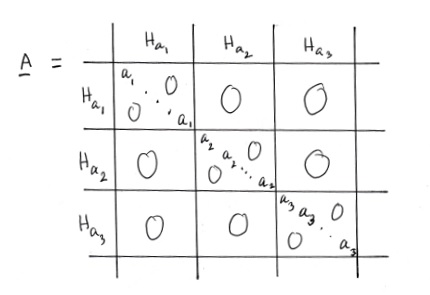
\includegraphics[scale=1.0]{A.jpg}
\vspace{-0.8 cm}
\caption{The matrix representation of $\hat{A}$ in the eigenbasis of $\hat{A}$. }
\label{fig:A}
\end{figure}

\noindent
where each diagonal block $H_{a_n}$ is a $g_{a_n}\times g_{a_n}$ dimensional diagonal matrix with the eigenvalue $a_n$ running
along the diagonal, other entries being zero.


\paragraph{}
Next, we ask what would be the matrix representation of $\hat{B}$ in the eigenbasis of $\hat{A}$. The matrix elements
of $\hat{B}$ are written as 
$\langle a^{\prime}, i^{\prime}|\hat{B}|a,i\rangle$. Using our assumption that $\hat{A}$ and $\hat{B}$ commute, we have
\be
\langle a^{\prime}, i^{\prime}|[\hat{A},\hat{B}]|a,i\rangle = 0,\nonumber
\ee
i.e.,
\be
\langle a^{\prime}, i^{\prime}|\hat{A}\hat{B}-\hat{B}\hat{A}|a,i\rangle = 0, \nonumber
\ee
or,
\be
(a^{\prime}-a)\langle a^{\prime}, i^{\prime}|\hat{B}|a,i\rangle=0.
\ee
If $a\neq a^{\prime}$, then $(a^{\prime}-a)\neq 0$ and we must have
\be
\langle a^{\prime}, i^{\prime}|\hat{B}|a,i\rangle =0, \quad {\rm if} \; a^{\prime}\neq a,
\label{eq:matrixelement}
\ee
i.e., $\hat{B}$ does not connect states with different eigenvalues of $\hat{A}$. In other words, $\hat{B}$ acting
on any of the eigenvectors of $\hat{A}$ in the eigensubspace $H_a$, produces another vector which is also in $H_a$ with no components in other eigensubspaces orthogonal to $H_a$. The new vector, being in $H_a$, remains an eigenvector of $\hat{A}$. Thus, $\hat{B}$
acting on any eigenvector of $\hat{A}$ produces a state which is also an eigenvector of $\hat{A}$ with the same eigenvalue. This is a
consequence of the fact that $\hat{A}$ and $\hat{B}$ commute.

\paragraph{}
From the above arguments, we can conclude that the matrix representation of $\hat{B}$ in the eigenbasis of $\hat{A}$
will be block diagonal as shown below.
\begin{figure}[h]
\centering
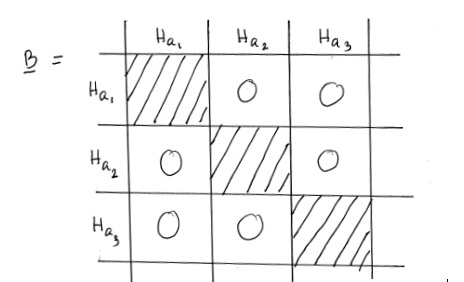
\includegraphics[scale=0.9]{B.jpg}
\vspace{-3 mm}
\caption{The matrix representation of $\hat{B}$ in the eigenbasis of $\hat{A}$. }
\label{fig:B}
\end{figure}

\noindent
In each eigensubspace $H_a$, the matrix ${\underline B}^{(a)}$ is a $g_a \times g_a$ square matrix, which itself need not be diagonal if we choose an arbitrary basis for $H_a$. To see this we refer to Eq. (\ref{eq:matrixelement}). This equation tells us that, 
if $\hat{A}$ and $\hat{B}$ commute, the matrix of elements of $B$ are zero if $a\neq a^{\prime}$, but nothing is concluded about
the matrix elements of $\hat{B}$ in any eigensubspace $H_a$, i.e., when $a=a^{\prime}$. 

\paragraph{}
However, since $\hat{B}$ is a Hermitian operator, its matrix representation in every eigensubspace $H_a$, is a finite dimensional square Hermitian matrix. We can always diagonalize a finite dimensional Hermitian matrix by a change of basis. The new set of $g_a$ basis vectors in the eigensubspace $H_a$ are linear combinations of the old basis vectors 
$\{ |a,i\rangle, i=1,2, \cdots , g_a\}$. Therefore, the vectors of the new basis set remain eigenvectors of $\hat{A}$ with the same eigenvalue $a$. But, the vectors in  new basis set, since it diagonalizes $\hat{B}$, must also 
be eignevectors of $\hat{B}$ with eigenvalues $b_1,b_2, \cdots, b_{g_a}$.

\paragraph{}
Since the vectors in the new basis set are simultaneous eigenvectors of $\hat{A}$ and $\hat{B}$, we can label them by the eigenvalues of both $\hat{A}$ and $\hat{B}$. Thus the common eigenvectors, which form the new basis set of $H_a$, can be written as
$\{ |a,b_1\rangle, |a,b_2\rangle, \cdots , |a, b_{g_a}\rangle \}$. Some of the eigenvalues of $\hat{B}$ may be repeated, in which 
case we will need another index to distinguish between the linearly independent simultaneous eigenvectors with the same eigenvalues for $\hat{A}$ and $\hat{B}$. We diagonalize each diagonal block $\underline{B}^{(a_i)}$ of the matrix 
$\underline{B}$ in the old basis, thereby obtaining simultaneous eigenvectors for both $\hat{A}$ and $\hat{B}$ in the entire Hilbert space. In the new basis consisting of the simultaneous eigenvectors,  the matrix representation of $\hat{B}$ is diagonal as shown in 
 figure (\ref{fig:C}).
\begin{figure}[h]
\centering
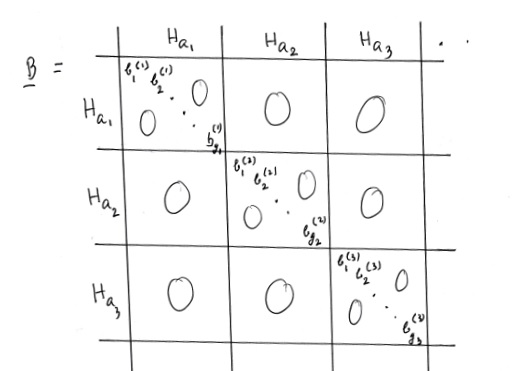
\includegraphics[scale=0.850]{C.jpg}
\vspace{-6 mm}
\caption{The matrix representation of $\hat{B}$ in the eigenbasis consisting of simultaneous eigenvectors of
$\hat{A}$ and $\hat{B}$.}
\label{fig:C}
\end{figure}

\noindent
The matrix representation of $\hat{A}$ in the new basis is also diagonal and remains the same as in Fig. (\ref{fig:A}). 

\paragraph{}
The diagonal entries $b_i^{(n)}, i=1,2, \cdots , g_n$ in each eigensubspace $H_{a_n}$ in figure (\ref{fig:C}) are the various eigenvalues of the operator $\hat{B}$, i.e., $b_i^{(n)} \in \{b_1,b_2, \cdots\}$. In a given eigensubspace $H_{a_n}$, some of the eigenvalues of
$\hat{B}$ may be repeated. Further, a particular eigenvalue of $\hat{B}$ may also be repeated in several eigensubspaces $H_{a_n}$.

\paragraph{}
Thus, in summary, what we have shown is that, given two Hermitian operators $\hat{A}$ and $\hat{B}$ representing
two observables of a quantum system,  it is possible to construct a complete set of simultaneous eigenvectors 
spanning the entire Hilbert space provided  $[\hat{A},\hat{B}]=0$. Hence, we have proved that $[\hat{A},\hat{B}]=0$ is a sufficient condition for two Hermitian operators $\hat{A}$ and $\hat{B}$ to be compatible.


% New section
% Sec 5
\section{Labeling of Quantum Mechanical Basis States}
Since eigenvectors of a Hermitian operator corresponding to an observable form a complete set, we can label the members of the set by the eigenvalues. Thus, suppose that an observable $\hat{A}$ has eigenvalues
\[ a_1, a_2, a_3, \cdots\, . \]
The basis states are then labeled as
\[ |a_1\rangle,\, |a_2\rangle,\, |a_3\rangle,\, \cdots \, . \]
The labeling would be unambiguous if the eigenvalues were all non-degenerate. However, if some or all eigenvalues are degenerate, we will need another mark of distinction for the eigenvectors. 

\paragraph{}
For example, if an eigenvalue $a_n$ is $g_n$-fold degenerate, the corresponding eigenvectors may be denoted as
\[ |a_n,i\rangle,\, i=1,2, \cdots , g_n\, . \]
An alternative, and better, notation is based on the fact that two compatible observables whose Hermitian operators commute, may be assumed to have the same set of eigenvectors. Hence, if we can find a second observable $\hat{B}$ commuting with the first, such that
\be
\hat{B}|a_n,i\rangle = b_i|a_n,i\rangle,\, i=1,2, \cdots , g_n 
\ee
with eigenvalues $b_i$ all different, then the eigenvalues of $\hat{B}$ may serve to distinguish the eigenvectors.
So, we can write
\[
\begin{array}{lcl}
|a_n,1\rangle & \equiv & |a_n,b_1\rangle \\
|a_n,2\rangle & \equiv & |a_n,b_2\rangle \\
. & & . \\
. & & . \\
. & & . \\
|a_n,g_n\rangle & \equiv & |a_n,b_{g_n}\rangle\, . 
\end{array}
\]
But, if some of the eigenvalues $b_i, i=1,2, \cdots, g_n$ are equal, we will need a third mark to distinguish the eigenvectors. The third mark may be obtained if we can find a third observable whose operator $\hat{C}$ commutes with both $\hat{A}$ and 
$\hat{B}$. Then $\hat{A}$, $\hat{B}$ and $\hat{C}$ have simultaneous eigenvectors and the eigenvalues of $\hat{C}$ may also be used to label the eigenvectors.

\paragraph{}
Thus, in general, if we can find a set of mutually commuting Hermitian operators, $\hat{A},\hat{B},\hat{C},\hat{D} , \cdots $
whose common eigenvectors can be characterized completely by the eigenvalues $a,b,c,d, \cdots$ such that no two eigenvectors have exactly identical set of eigenvalues, then the eigenvalues of these operators can uniquely label the common eigenvectors.
Such a set of Hermitian operators is said to be complete. We refer to this set of operators as a complete set of commuting 
observables (CSCO). 

\paragraph{}
In the new notation, the basis vectors are written as
\[ |a,b,c, d, \, \cdots \rangle \, . \]
The normalization and completeness conditions are then 
\be
\langle a^{\prime},b^{\prime},c^{\prime}, d^{\prime} \cdots |a,b,c,d,\cdots \rangle = \delta_{aa'}\delta_{bb'} \cdots \, ,
\ee
and
\be
\sum_{(a,b,c,d,\cdots)} |a,b,c,d,\cdots \rangle \langle a,b,c,d,\cdots |= \hat{I} \, . 
\ee













\setcounter{chapter}{8}
\noindent
\begin{Large}
{\bf Lecture 8 \newline
Compatibility of Observable: version 2}
\end{Large}

\section{Background Materials}
Suppose that $\hat{A}$ is the Hermitian operator representing an observable A of a quantum system. The eigenkets of ${\hat A}$
form a complete set of orthonormal basis states. Let $|\psi\rangle$ be the state vector of the system. We can expand 
$|\psi\rangle$ in the eigenbasis of the operator ${\hat A}$:
\be
|\psi\rangle = \sum_a |a\rangle \langle a|\psi\rangle \, , 
\label{eq:1}
\ee
where $a$ runs over all the eigenvalues of ${\hat A}$, i.e., $a\in {\rm spec}(\hat{A})$, where ${\rm spec}\,(\hat{A}) =
(a_1,a_2, a_3, \ldots )$ is the set of all eigenvalues of $\hat{A}$. This set is called the eigenvalue spectrum of $\hat{A}$.


\paragraph{}
In Eq. (\ref{eq:1}), we have assumed that each eigenvalue $a$ is non-degenerate, i.e., for each $a$ there exists only one linearly independent eigenvector $|a\rangle$. Therefore, the eigenvalue itself can be used to label the corresponding eigenket unambiguously.

\paragraph{}
However, it may so happen that some or all of the eigenvalues of ${\hat A}$ are degenerate, i.e., there may be more than one linearly independent eigenvector corresponding to the same eigenvalue. The number of linearly independent eigenvectors corresponding
to a particular eigenvalue $a$ is called the order of degeneracy of the eigenvalue and is denoted by $g_a$. If the eigenvalue $a$ is degenerate, then just the eigenvalue itself is not enough to label the eigenstates uniquely. We need another index to distinguish between the $g_a$ linearly independent eigenvectors all with the same eigenvalue $a$.

\paragraph{}
Thus the eigenvectors belonging to a degenerate eigenvalue $a$ may be denoted by $|a,i\rangle$, where the index $i$ 
can take discrete values $i=1,2,3, \cdots , g_a$. The index $i$ may be called the degeneracy index. Later, we will see that we can improve the notation by replacing $i$ by the eigenvalues of other Hermitian operators $\hat{B}$, $\hat{C},\, \cdots$, which commute
with $\hat{A}$. 

\paragraph{}
The set of linearly independent eigenvectors $\{ |a,i\rangle, i=1,2, \cdots, g_a\}$, all with the same eigenvalue $a$, span a $g_a$-dimensional subspace of the Hilbert space. This subspace is called the eigensubspace of $a$, and is denoted by $H_a$. The union of all the eigensubspaces of the operator $\hat{A}$ constitutes the full Hilbert space.

\paragraph{}
It is easy to see that any linear combination of the eigenvectors $\{ |a,i\rangle, i=1,2, \cdots, g_a\}$ is also an eigenvector of $\hat{A}$ with the same eigenvalue $a$. Thus
\be
\hat{A} \left( \sum_{i=1}^{g_a} c_i |a,i\rangle\right) = a \left(\sum_{i=1}^{g_a} c_i |a,i\rangle\right)\,,
\ee
where $c_i$'s are constants.
The set of eigenvectors $\{ |a,i\rangle, i=1,2, \cdots, g_a\}$, even though linearly independent, may not be orthogonal to each other
because they belong to the same eigenvalue. However, following the Schmidt orthonormalization procedure, we can take linear combinations of the above set of vectors in a special way and obtain a set of $g_a$ orthonormal vectors. The new set of orthonormal (and hence also linearly independent ) vectors remain eigenvectors of $\hat{A}$ with the same eigenvalue $a$. 

\paragraph{}
We assume that the Schmidt procedure has been carried out in each eigensubspace. So, in each eigensubspace, we can write
\be 
\langle a,i|a,j\rangle = \delta_{ij} , \;\; a\in {\rm Spec}(\hat{A})
\ee
where $i,j = 1,2,3, \cdots , g_a$. 
The orthonormal set of eigenvectors $\{ |a,i\rangle, i= 1,2, \cdots , g_a\}$ can be said to span the eigensubspace $H_a$.
The eigenvectors in different eigensubspaces are automatically orthogonal because $\hat{A}$ is Hermitian. Hence, we can assume that 
{\bf all}  eigenvectors of $\hat{A}$ are orthonormal, i.e.,
\be
\langle a^{\prime}, i^{\prime}|a,i \rangle = \delta_{aa^{\prime}}\delta_{ii^{\prime}} \, .
\ee
The full set $\{ |a, i\rangle, i=1,2, \cdots , g_a;\, a\in {\rm spec}\,(\hat{A}) \}$ of eigenvectors of $\hat{A}$ form a complete 
orthonormal set, i.e., they constitute a basis set for the Hilbert space. The completeness condition of this basis set can be written as 
\be 
\sum_{a\in {\rm spec}\,(\hat{A})}\sum_{i=1}^{g_a} |a,i \rangle \langle a,i| = \hat{I}\, .
\ee
Thus the state vector $|\psi\rangle$ of the system can be expanded as
\begin{eqnarray}
|\psi\rangle & = & \hat{I} |\psi\rangle \nonumber \\
             & = & \sum_{a\in {\rm spec}\,(\hat{A})}\sum_{i=1}^{g_a} |a,i \rangle \langle a,i|\psi\rangle\, .
\end{eqnarray}			

\paragraph{}
For simplicity, we will continue to use Eq. (\ref{eq:1}) as the expansion for $|\psi\rangle$ in the eigenbasis of $\hat{A}$
assuming that all the eigenvalues are non-degenerate. In case of degeneracy, notations can be generalized in a straightforward manner, as discussed above.			



% Section 2
\section{Measurement of Two Observables in Quick Succession}
Suppose that a quantum system is in the state $|\psi\rangle$. Let $A$ be an observable of the system with corresponding Hermitian operator $\hat{A}$. We can always expand $|\psi\rangle$ using the eigenbasis of $\hat{A}$:
\be
|\psi\rangle = \sum_a |a\rangle \langle a|\psi\rangle \, ,
\ee
where $a$ runs over the eigenvalue spectrum of $\hat{A}$. The complex number $\langle a |\psi\rangle$ is the `component' of 
$|\psi\rangle$ along $|a\rangle$. 

\paragraph{}
We now make a measurement of the observable $A$ on the system in the state $|\psi\rangle$. Since a general state $|\psi\rangle$
may be a superposition of many (perhaps infinitely many) eigenkets of $\hat{A}$ with different eigenvalues, we cannot exactly 
predict the result of the experiment but can only say that the experiment would yield one of the eigenvalues 
of $\hat{A}$ for which $\langle a|\psi\rangle \neq 0$. 

\paragraph{}
The outcome is random, i.e., probabilistic, because we cannot predict exactly which eigenvalue will be obtained, but we can assign a probability for obtaining a particular eigenvalue $a$ provided we know the state $|\psi\rangle$ before the measurement.
The probability is
\be
P_{|\psi\rangle}(a) = \left|\langle a|\psi\rangle \right|^2 \, . 
\ee
In the course of the measurement, the state of the system collapses to the eigenket $|a\rangle$ if the eigenvalue $a$ is obtained in the measurement. Thus
\be
|\psi\rangle\;\; \xrightarrow{{\rm measurement\; of\; A} }\;\; |a\rangle.
\ee
Now the system is in a state with a definite value for the observable $A$. Further successive measurements of $A$ will yield the same eigenvalue $a$ with 100\% certainty. 

\paragraph{}
Next, consider another observable $B$ of the system with corresponding Hermitian operator $\hat{B}$. If, immediately after the  measurement of $A$, we measure B, are we certain to get a particular eigenvalue $b$ of the operator $\hat{B}$?
We know that the state of the system after the measurement of $A$ is an eigenstate of $\hat{A}$, i.e., in a state with a definite value $a$ of the observable $A$. The question we have asked can be restated as follows: in the collapsed state
$|a\rangle$, does $B$ have a definite value, i.e., is $|a\rangle$ also an eigenstate of $\hat{B}$  with some eigenvalue $b$? The answer to this question is, in general, in the negative, i.e., $|a\rangle$ is not an eigenket of $\hat{B}$ in general. The very important exceptional case 
where $|a\rangle$ is also an eigenstate of $\hat{B}$ is discussed later.

\paragraph{}
Since the eigenkets of $\hat{B}$  form a basis set, we can expand $|a\rangle$ as
\be
|a\rangle = \sum_b |b\rangle \langle b|a\rangle \, .
\ee
Therefore, a measurement of $B$ would yield any one of the eigenvalues $b\in {\rm spec}\,(\hat{B})$ for which $\langle b |a\rangle \neq 0$.
The probability of obtaining a particular eigenvalue $b$ while the system is in the state $|a\rangle$ is
\be
P_{|a\rangle}(b) = \left | \langle b | a\rangle \right|^2 \, .
\ee
The state of the system after B is measured collapses from $|a\rangle$ to $|b\rangle$:
\be
|a\rangle\;\; \xrightarrow{{\rm measurement\; of\; B} }\;\; |b\rangle.
\ee
Thus, the measurement of $B$ generally alters the state of the system just before the measurement because, due to the measurement process, the system is thrown into the eigenstate $|b\rangle$, where $b$ is the eigenvalue of  $\hat{B}$ obtained in the measurement. But, since $|b\rangle$ is not, in general, an eigenstate of $\hat{A}$, the system is no longer in a state with a definite value for the observable  $A$.

\paragraph{}
If we measure $A$ again immediately after $B$ is measured, we will not get the answer we got the first time, namely $a$, with certainty. In the second measurement of $A$ there is the possibility of getting any eigenvalue for which $\left| \langle a|b\rangle\right| \neq 0$. To repeat,  after the first measurement of $A$, the system is in the eigenstate $|a\rangle$ of
$\hat{A}$ but this state is not an eigenstate of the operator $\hat{B}$ except in a special situation discussed below. After the measurement of $B$, the system is thrown in the eigenstate $|b\rangle$ of $\hat{B}$ which is not an eigenstate of $\hat{A}$. Therefore, it is not possible, in general, to get the system in a state in which both the observables $A$ and $B$  have definite values.

\paragraph{}
Now, in successive measurements of $A$ and $B$, first $A$ then $B$, on a system initially in the state $|\psi\rangle$, the probability of obtaining the result $a$ and $b$ is
\be
P(a,b) = P_{|\psi\rangle}(a) P_{|a\rangle}(b) = \left|\langle a|\psi\rangle\right|^2\left| \langle b|a\rangle\right|^2\, .
\ee
If we reversed the order of measurements, first $B$ and then $A$,  the probability for obtaining the results
$b$ for the observable $B$ and $a$ for the observable $A$ would be
\be
P(b,a) = P_{|\psi\rangle}(b) P_{|b\rangle}(a) = \left|\langle b|\psi\rangle\right|^2\left| \langle a|b\rangle\right|^2\, .
\ee
We note that, since $\left|\langle a|\psi\rangle\right|^2\neq \left|\langle b|\psi\rangle\right|^2$, the two probabilities are not equal in general, 
i.e., $P(a,b)\neq P(b,a)$.


% New Section

\section{Compatible Observables}
Now, let us return to the exceptional situation mentioned in the previous section. To recapitulate, let us make two 
measurements of two observables $A$ and $B$ in quick succession on a system in the state $|\psi\rangle$. First, we measure $A$, and if the eigenvalue $a$ is obtained, the system's state collapses to an eigenstate of the operator $\hat{A}$ belonging to the eigenvalue $a$. Then if we measure $B$ immediately afterward, would we be certain to get a particular eigenvalue $b$ of $\hat{B}$? Further, if a second measurement of $A$ is made immediately after the measurement of $B$, what conditions need be fulfilled in order that the result of the first measurement is unaltered, i.e., we will be certain to get the same result $a$ again? We will first consider the case when all eigenvalues of $\hat{A}$  and 
$\hat{B}$ are non-degenerate and then we will consider degeneracy of the eigenvalues. 

\subsection {Nondegenerate Case}
Suppose all eigenvalues of $\hat{A}$ and $\hat{B}$ are nondegenerate. First we measure $A$ on a system which 
is initially in the state $|\psi\rangle$. The system's initial state $|\psi\rangle$ collapses to the eigenstate 
$|a\rangle$ if the eigenvalue $a$ is obtained in the measurement of $A$. In general, the observable $B$ does not have a definite value in the state $|a\rangle$.

\paragraph{}
An exception occurs if $|a\rangle$ is also an eigenstate of $\hat{B}$ with some eigenvalue $b$, i.e., 
\be
\hat{B}|a\rangle = b |a\rangle \, . 
\ee
Since $|a\rangle$ is an eigenvector of both $\hat{A}$ and $\hat{B}$ with eigenvalues $a$ and $b$, respectively, it is more expressive to label the eigenket by both the eigenvalues, i.e.,
\[ |a\rangle \equiv |a,b\rangle\, . \]
Hence 
\be
\hat{A}|a,b\rangle = a |a,b\rangle
\ee
and
\be
\hat{B}|a,b\rangle = b|a,b\rangle\, .
\ee
Now, the measurement of $B$ immediately after $A$, is certain to yield $b$ and the state of the system would remain unaltered due to the $B$-measurement. The change of the state of the system in the two measurements is shown below:
\[ |\psi\rangle \xrightarrow{{\rm Measure} \; \hat{A}}\; |a,b\rangle\; \xrightarrow{{\rm Measure} \; \hat{B}}\; |a,b\rangle \, . \]
There is no change of the state of the system due to the measurement of $B$ because the system was already in an eigenstate of 
$\hat{B}$
prior to the measurement. Since the state of the system has collapsed to a simultaneous eigenstate of both $\hat{A}$ and
$\hat{B}$ after the measurement of $A$, the system is now in a state where both the observables have definite values, namely, $a$ 
and $b$. Further, since the measurement of $B$ does not alter the state, a second measurement of $A$ is certain to yield the previous value $a$. 

\paragraph{}
If the scenario just described holds in all situations, no matter what is the outcome of the first measurement of $A$, we say that the observables $A$ and $B$ are compatible. Thus, in summary, if we perform the following sequence of measurements in rapid succession on a system:
\begin{quote}
1. measure $A$ ~~~ 2. measure $B$ ~~~ 3. remeasure $A$
\end{quote}
then, if the result of 3 is certain to be the same as the result of 1, we say that $A$ and $B$ are compatible variables. The condition for compatibility in the nondegenerate case is that every eigenvector of $\hat{A}$ is also an eigenvector of $\hat{B}$
so that the common eigenvectors form a basis of the Hilbert space. Therefore, if observables $A$ and $B$ are compatible, it is always possible to find states of the system, namely the simultaneous eigenstates of $\hat{A}$ and $\hat{B}$, in which both the observables
have definite values.

\paragraph{}
Next, if $A$ and $B$ are compatible, the probability of getting the results $a$ and $b$ in the sequence
of measurements: $A$ followed by $B$,  would be
\be 
P(a,b) = P_{|\psi\rangle}(a) P_{|a,b\rangle}(b) = \left| \langle a,b|\psi\rangle \right|^2 \times 1 = \left| \langle a,b|\psi\rangle \right|^2\, .
\ee
If we reverse the order of measurements and assume that the eigenvalues of $\hat{B}$ are also nondegenerate like those of 
$\hat{A}$, then $P(b,a)$ would be the same as $P(a,b)$. For non-compatible observables $P(a,b)$ would not be equal to $P(b,a)$.






\subsection{Degenerate Case}
Let us next consider the general case where the eigenvalues of both $\hat{A}$ and $\hat{B}$ may be degenerate. As before, we measure $A$ and $B$ in rapid succession, in the order
$A$ then $B$, on a system in the state $|\psi\rangle$. If a particular eigenvalue $a$ of the operator $\hat{A}$ is
obtained in the measurement, the state of the system collapses to the normalized projection of $|\psi\rangle$ onto the eigensubspace $H_a$ i.e.,
\be
|\psi\rangle \xrightarrow{{\rm Measure}\; A} \, |\psi^{\prime}\rangle = \frac{\hat{P}_a|\psi\rangle}
{\sqrt{ \langle \psi|\hat{P}_a|\psi\rangle}} \in H_a \, .
\ee
The eigensubspace $H_a$ is $g_a$-dimensional. The basis vectors of $H_a$ could be chosen as the $g_a$ linearly independent eigenvectors 
of $\hat{A}$  with the same eigenvalue $a$, i.e. $\{|a,i\rangle, i = 1,2, \cdots , g_a\}$.  In terms of these basis vectors the projection operator $\hat{P}_a$ onto $H_a$ is written as
\be
\hat{P}_a = \sum_{i=1}^{g_a}|a,i\rangle \langle a,i|.
\ee
Any vector in $H_a$  (infinitely many of them) is an eigenvector of $\hat{A}$ with eigenvalue $a$, but there are only $g_a$ linearly independent vectors 
in $H_a$. 


\paragraph{}
A subsequent measurement of $B$ yielding some
 eigenvalue $b$ will throw the system into the normalized projection of $|\psi^{\prime}\rangle$  onto the eigensubspace $H_b$, i.e.,
\[ |\psi^{\prime}\rangle \xrightarrow{{\rm Measure}\; B} |\psi^{\prime \prime}\rangle \in H_b.\]
The state $|\psi^{\prime \prime}\rangle$ lying in the 
eigensubspace $H_b$,  will in general have components both in $H_a$ and $H_a^{ \bot}$, where $H_a^{ \bot}$, called the orthogonal complement 
of $H_a$, is the subspace orthogonal to $H_a$. The subspace $H_a^{ \bot}$ consists of (is the union of) the eigensubspaces 
of $\hat{A}$ other than $H_a$. So, a second measurement of $A$ will not yield $a$, the value obtained in the first measurement, with certainty, i.e., $A$ and $B$ would be incompatible.


% Here Kabir
\paragraph{}
However, in exceptional cases it may be possible to find $g_a$ linearly independent eigenvectors of the operator $\hat{B}$
with  eigenvalues $b_1, b_2, \cdots$ (some $b_i$'s may be repeated) in each eigensubspace $H_{a}$ and, being  linearly independent, the eigenvectors can span the eigensubspace $H_a$. These eigenvectors of $\hat{B}$, since they lie wholly in $H_{a}$, are also eigenvectors of $\hat{A}$ with the same eigenvalue $a$. We may denote these simultaneous eigenvectors
of $\hat{A}$ and $\hat{B}$ in $H_a$ as follows:
\be
|a, b^{\prime}, i_{(ab^{\prime})} \rangle, \, i_{(ab^{\prime})} =1,2, \cdots , g_{(ab^{\prime})}, \, b^{\prime}= b_1,b_2,\ldots. \,. 
\label{eq:simab}
\ee
Here $g_{(ab^{\prime})}$ is the order of degeneracy of the eigenvalue $b^{\prime}$ in the eigensubspace $H_a$, or, in other words, the order of degeneracy of the eigenavalue pair $(ab^{\prime})$ in the full Hilbert space $H$. The order of degeneracy of $b^{\prime}$ in the entire Hilbert space may be greater, for some of the linearly independent eigenvectors of $\hat{B}$  with the same degenerate eigenvalue  
$b^{\prime}$ may lie in eigensubspaces other that $H_a$. 

\paragraph{}
Thus, in the special case we are considering, we can find simultaneous eigenvectors of both $\hat{A}$ and $\hat{B}$ which span each eigensubspace $H_a$ and so the whole Hilbert space can also be spanned by simultaneous eigenvectors of the two operators. 

\paragraph{}
In terms of the simultaneous eigenvectors of $\hat{A}$ and $\hat{B}$, we can write $|\psi^{\prime}\rangle$ as
\begin{eqnarray}
|\psi^{\prime}\rangle &=& N^{\prime} \hat{P}_a |\psi\rangle \nonumber \\
&=&  N^{\prime} \sum_{b^{\prime}=b_1, b_2, \ldots}\,\sum_{i_{(ab^{\prime}})=1}^{g_{ (ab^{\prime})    }} |a,b^{\prime},i_{(ab^{\prime})}\rangle
\langle a,b^{\prime},i_{(ab^{\prime})}|\psi\rangle
\end{eqnarray}
where $N^{\prime}$ is the normalization constant for $|\psi^{\prime}\rangle$, i.e.,
\be
N^{\prime}= \frac{1}{\sqrt{ \sum_{b^{\prime}=b_1, b_2, \ldots}\,\sum_{i_{(ab^{\prime}})=1}^{g_{ (ab^{\prime})    }}{ |\langle a,b^{\prime},i_{(ab^{\prime})}|\psi\rangle|^2}}}
=\frac{1}{ \sqrt{ \langle \psi|\hat{P}_a|\psi\rangle } }.
\ee

\paragraph{}
Next, if we measure $B$ immediately after $A$, we have non zero probability of getting one of the eigenvalues $b_i$ that appears in the basis set
$|a, b^{\prime}\in\{b_1,b_2, \ldots\}, i_{ab^{\prime}}\rangle$ that spans $H_a$. Suppose we get a particular value $b_i$. The state of the system then collapses 
into $|\psi^{\prime \prime}\rangle$ which is the normalized projection of $|\psi^{\prime}\rangle$ onto $H_{b_i}$, i.e.,
\be
|\psi^{\prime}\rangle \xrightarrow{{\rm Measure}\; B}  |\psi^{\prime \prime}\rangle  =  N^{\prime\prime} \hat{P}_{b_i}\hat{P}_a |\psi\rangle
\label{eq:psipp}
\ee
where $N^{\prime\prime}$ is the normalization constant for $|\psi^{\prime \prime}\rangle$. The projection operator on the eigensubspace $H_{b_i}$ can be written as 
\be
\hat{P}_{b_i}= \sum_{a^{\prime}} \sum_{\alpha_{(a^{\prime}b_i)}=1}^{ g_{(a^{\prime}b_i)}} |a^{\prime}, b_i, \alpha_{(a^{\prime}b_i)}\rangle 
\langle a^{\prime}, b_i, \alpha_{(a^{\prime}b_i)}|
\ee
where $\alpha_{(a^{\prime}b_i)}$ is the degeneracy index for the eigenvalue pair $(a^{\prime}b_i)$.
Noting the basis vectors are orthonormal, we have
\be
\hat{P}_{b_i}\hat{P}_a = \sum_{\alpha_{ (ab_i)}=1}^{g_{(ab_i)}} |a, b_i, \alpha_{(ab_i)}\rangle \langle a, b_i, \alpha_{(ab_i)}|.
\ee
The vector $|\psi^{\prime \prime}\rangle $ immediately after the measurement of $B$ given in Eq. (\ref{eq:psipp}) can now be written as
\be
|\psi^{\prime \prime}\rangle = N^{\prime\prime} \sum_{\alpha_{ (ab_i)}=1}^{g_{(ab_i)}} |a, b_i, \alpha_{(ab_i)}\rangle \langle a, b_i, \alpha_{(ab_i)}|\psi\rangle.
\ee
The normalization constant $N^{\prime \prime}$ is
\be
N^{\prime \prime}=\frac{1}{\sqrt{ \sum_{\alpha_{ (ab_i)}=1}^{g_{(ab_i)}} |\langle a, b_i, \alpha_{(ab_i)}|\psi\rangle|^2  }    }=
\frac{1}{\sqrt{\langle \psi|\hat{P}_{b_i}\hat{P}_a |\psi\rangle}}
\ee

\paragraph{}
We note that the measurement of $B$ has changed the state from $|\psi^{\prime}\rangle$ to $|\psi^{\prime\prime}\rangle$, unlike in the nondegenerate case, but the changed state is still in $H_a$. So, a second measurement of $A$ would certainly
 give the same eigenvalue $a$ as was obtained in the first measurement of the observable. 
Therefore, the observables  $A$ and $B$ are compatible. Further, the state $|\psi^{\prime \prime}\rangle$ is a simultaneous eigenstate of both $\hat{A}$
and $\hat{B}$. So, in the the state $|\psi^{\prime \prime}\rangle$, both the observables $A$ and $B$ have definite values, namely $a$ and $b_i$, respectively.

\paragraph{}
To summarize, if in every  eigensubspace $H_a$ of the eigenvalues of $\hat{A}$, it is possible to find $g_a$ linearly independent of eigenvectors of the operator $\hat{B}$, then the totality of all the simultaneous eigenvectors in the entire Hilbert space form a complete basis set of vectors. The two observables would then be compatible. 


\paragraph{}
This is not to say that any eigenvector 
of $\hat{A}$ is also an eigenvector of $\hat{B}$. For example, if we take any vector in $H_a$, the vector is guaranteed to be an eigenvector of $\hat{A}$, but not necessarily an eigenvector of $\hat{B}$. To see this let us consider the vector
\be
|\psi\rangle = c_1|a,b_1\rangle + c_2|a,b_2\rangle \in H_a\, .
\ee
This is a vector in $H_a$ and therefore an eigenvector of $\hat{A}$ with eigenvalue $a$, but not an eigenvector of $\hat{B}$. 
There are infinity of different vectors in $H_a$ but only $g_a$ linearly independent ones which can act as basis for $H_a$. 
These linearly independent vectors,  though eigenvectors of $\hat{A}$ with eigenvalue $a$, may not in general  be eigenvectors of $\hat{B}$ also. However, by taking appropriate linear combinations of these linearly independent eigenvectors if it is
possible to get another set of $g_a$ linearly independent vectors which are also eigenvectors of $\hat{B}$, then the two observables are compatible. Therefore, for two observables to be compatible, they must have simultaneous eigenvectors which form
a complete set of basis states for the Hilbert space.




% Sec 4														
\section{Condition for Compatibility of Observables}
In the previous section we have stated what we mean when we say two observables are compatible with each other.
To recapitulate, if two observables have simultaneous eigenvectors that span the entire Hilbert space, i.e., if the simultaneous 
eigenvectors form a basis for the Hilbert space, then the observables are said to be compatible.

\paragraph{} 
We will now prove that two observables $A$ and $B$ with corresponding Hermitian operators $\hat{A}$ and $\hat{B}$, respectively,  
 are compatible if and only if $[\hat{A},\hat{B}]=0$. Thus we prove the following theorem:

\subsubsection{Theorem: }
Two Hermitian operators representing two observables have a complete set of simultaneous eigenvectors if and only if they commute.

\noindent An alternative statement of the theorem could be: The necessary and sufficient condition that two observables are compatible is that their operators commute.

\subsubsection{Proof:}
The proof proceeds in two parts. First, we prove the necessary condition, i.e., we assume that that the operators have simultaneous eigenvectors, then we show that the operators commute. Next, we prove the converse (the sufficiency condition), i.e., we assume that
the operators commute, then we show they have simultaneous eigenvectors.

\newpage
\noindent
{\bf {\underline {(a) Necessary Condition}}}

Let us assume that $\hat{A}$ and $\hat{B}$ have a complete set of simultaneous eigenvectors $|u_n\rangle, n =1,2, \cdots$. Here each $u_n$ represents a unique set of numbers
 $\{a_n,b_n,\alpha_{(a_nb_n)}\}$, where $a_n$ and $b_n$ are eigenvalues of $\hat{A}$ and $\hat{B}$, respectively, and $\alpha_{(a_nb_n)}$ is any other parameter which would be required to label the states uniquely should there be more than one linearly independent eigenvectors with the same values for the pai $(a_nb_n)$. Since the complete set of vectors 
$\{|u_n\rangle,\, n= 1,2, \cdots\}$ are eigenvectors of both
$\hat{A}$ and $\hat{B}$, we have
\be
\hat{A}|u_n\rangle = a_n |u_n\rangle\, ,
\label{eq:A}
\ee
and
\be
\hat{B}|u_n\rangle = b_n |u_n\rangle\, .
\label{eq:B}
\ee
Now, using Eq. (\ref{eq:A}) and (\ref{eq:B}), we can write
\begin{eqnarray}
[\hat{A},\hat{B}]|u_n\rangle &= & (\hat{A}\hat{B}-\hat{B}\hat{A}]|u_n\rangle \nonumber \\
                             &=& (a_nb_n-b_na_n)|u_n\rangle \nonumber \\
														 & = & 0\,.
\end{eqnarray}
Since the simultaneous eigenvectors $\{|u_n\rangle, i= 1,2, \cdots\}$ form a complete set, it follows that
\be
[\hat{A},\hat{B}]|\psi\rangle = 0\, ,
\ee
where $|\psi\rangle$ is an arbitrary vector in the Hilbert space. Hence we have
\be
[\hat{A},\hat{B}] = 0\, .
\ee
Thus, we have proved that commutivity is a necessary condition for compatibility.


\vspace{3 mm}

\noindent
{\bf {\underline {(b) Sufficiency Condition}}}

We now prove the converse, i.e., if $\hat{A}$ and $\hat{B}$ commute, they have simultaneous eigenvectors.
First, we will assume that all eigenvalues of $\hat{A}$ are non-degenerate. Next, we will consider 
the more general situation, namely that, some or all of the eigenvalues of $\hat{A}$ may be degenerate.

\subsubsection{Non-degenerate case}
If all eigenvalues of $\hat{A}$ are non-degenerate, then it is possible to uniquely label the eigenstates of $\hat{A}$ by
the eigenvalues only. Thus let $|a\rangle$ be the eigenstate of the operator $\hat{A}$ belonging to some eigenvalue $a$. Therefore,
\begin{equation}
\hat{A}|a\rangle = a |a\rangle\, .
\label{eq:aa}
\ee
We start the proof by applying the operator $\hat{B}$ to Eq. (\ref{eq:aa}) to get
\be
\hat{B}\hat{A}|a\rangle = a\hat{B}|a\rangle\, .
\ee
Since our assumption is that $\hat{A}$ and $\hat{B}$ commute, we can interchange the order of $\hat{A}$ and $\hat{B}$ on the left hand side
of the above equation getting
\be
\hat{A}(\hat{B}|a\rangle)= a(\hat{B}|a\rangle)\, . 
\label{eq:ab}
\ee 
From Eq. (\ref{eq:ab})  we can conclude that $\hat{B}|a\rangle$ is also an eigenvector of $\hat{A}$ with the same 
eigenvalue $a$. Since we have supposed the eigenvalues of $\hat{A}$ are non-degenerate, the vectors $|a\rangle$ and
$\hat{B}|a\rangle$ represent the same physical state, i.e., $\hat{B}|a\rangle$ differs from $|a\rangle$ by a constant 
multiplier which we denote by $b$. Therefore,
\be
\hat{B}|a\rangle = b|a\rangle\, ,
\ee
i.e., all eigenvectors $\{ |a\rangle\}$ of ${\hat A}$ are also eigenvectors of $\hat{B}$. Therefore, we may label these states
by both eigenvalues $a$ and $b$, rather than the single eigenvalue $a$, i.e., $|a\rangle \equiv |a,b\rangle$.



% Kabir
\subsubsection{Degenerate Case}
Now, we allow for the more general case that some or all eigenvalues of $\hat{A}$
may be degenerate. In case of degeneracy, the eigenvalue equation for a particular eigenvalue $a$ is written as 
\be
\hat{A} |a,i\rangle = a|a,i\rangle ; \, i=1,2, \cdots , g_a\, ,
\ee
where $g_a$ is the order of degeneracy of $a$. Here $a$ is an element of the set of all the eigenvalues
of $\hat{A}$, i.e., $a\in\{a_1,a_2,\cdots\}$. The $g_a$ linearly independent eigenvectors $\{|a,i\rangle;\, i=1,2, \cdots, g_a\}$
spanning the eigensubspace $H_a$ are made orthonormal. 

\paragraph{}
If we choose the eigenvectors of $\hat{A}$ belonging to all the eigensubspaces, i.e., the set of eigenvectors
$\{|a,i\rangle, i=1,2,\cdots,g_a;\,a=a_1,a_2, \cdots\}$, as the basis for the Hilbert space, then obviously, the matrix
representation of $\hat{A}$ is diagonal. Denoting the matrix representing the operator $\hat{A}$ by $\underline{A}$, we have


\begin{figure}[h]
\centering
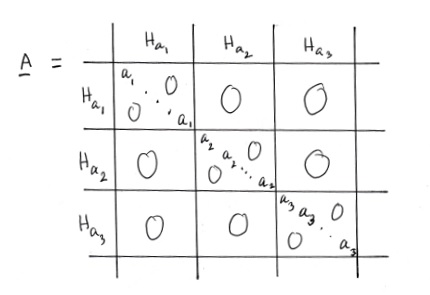
\includegraphics[scale=0.90]{A.jpg}
\vspace{-0.8 cm}
\caption{The matrix representation of $\hat{A}$ in the eigenbasis of $\hat{A}$. }
\label{fig:A}
\end{figure}

\noindent
where each diagonal block $H_{a_n}$ is a $g_{a_n}\times g_{a_n}$ dimensional diagonal matrix with the eigenvalue $a_n$ running
along the diagonal, other entries being zero.


\paragraph{}
Next, we ask what would be the matrix representation of $\hat{B}$ in the eigenbasis of $\hat{A}$. The matrix elements
of $\hat{B}$ are written as 
$\langle a^{\prime}, i^{\prime}|\hat{B}|a,i\rangle$. Using our assumption that $\hat{A}$ and $\hat{B}$ commute, we have
\be
\langle a^{\prime}, i^{\prime}|[\hat{A},\hat{B}]|a,i\rangle = 0,\nonumber
\ee
i.e.,
\be
\langle a^{\prime}, i^{\prime}|\hat{A}\hat{B}-\hat{B}\hat{A}|a,i\rangle = 0, \nonumber
\ee
or,
\be
(a^{\prime}-a)\langle a^{\prime}, i^{\prime}|\hat{B}|a,i\rangle=0.
\ee
If $a\neq a^{\prime}$, then $(a^{\prime}-a)\neq 0$ and we must have
\be
\langle a^{\prime}, i^{\prime}|\hat{B}|a,i\rangle =0, \quad {\rm if} \; a^{\prime}\neq a,
\label{eq:matrixelement}
\ee
i.e., $\hat{B}$ does not connect states with different eigenvalues of $\hat{A}$. In other words, $\hat{B}$ acting
on any of the eigenvectors of $\hat{A}$ in the eigensubspace $H_a$, produces another vector which is also in $H_a$ with no components in other eigensubspaces orthogonal to $H_a$. The new vector, being in $H_a$, remains an eigenvector of $\hat{A}$. Thus, $\hat{B}$
acting on any eigenvector of $\hat{A}$ produces a state which is also an eigenvector of $\hat{A}$ with the same eigenvalue. This is a
consequence of the fact that $\hat{A}$ and $\hat{B}$ commute.

\paragraph{}
From the above arguments, we can conclude that the matrix representation of $\hat{B}$ in the eigenbasis of $\hat{A}$
will be block diagonal as shown below.
\begin{figure}[h]
\centering
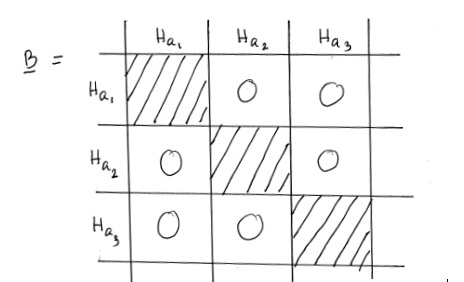
\includegraphics[scale=1.0]{B.jpg}
\vspace{-3 mm}
\caption{The matrix representation of $\hat{B}$ in the eigenbasis of $\hat{A}$. }
\label{fig:B}
\end{figure}

\noindent
In each eigensubspace $H_a$, the matrix ${\underline B}^{(a)}$ is a $g_a \times g_a$ square matrix, which itself need not be diagonal if we choose an arbitrary basis for $H_a$. To see this we refer to Eq. (\ref{eq:matrixelement}). This equation tells us that, 
if $\hat{A}$ and $\hat{B}$ commute, the matrix elements of $B$ are zero if $a\neq a^{\prime}$, but nothing is concluded about
the matrix elements of $\hat{B}$ in any eigensubspace $H_a$, i.e., when $a=a^{\prime}$. 

\paragraph{}
However, since $\hat{B}$ is a Hermitian operator, its matrix representation in every eigensubspace $H_a$, is a finite dimensional square Hermitian matrix. We can always diagonalize a finite dimensional Hermitian matrix by a change of basis. The new set of $g_a$ basis vectors in the eigensubspace $H_a$ are linear combinations of the old basis vectors 
$\{ |a,i\rangle, i=1,2, \cdots , g_a\}$. Therefore, the vectors of the new basis set remain eigenvectors of $\hat{A}$ with the same eigenvalue $a$. But, the vectors in  new basis set, since it diagonalizes $\hat{B}$, must also 
be eignevectors of $\hat{B}$ with eigenvalues $b_1,b_2,b_3, \cdots$ where some of the $b_i's$ may be repeated.

\paragraph{}
Since the vectors in the new basis set are simultaneous eigenvectors of $\hat{A}$ and $\hat{B}$, we can label them by the eigenvalues of both $\hat{A}$ and $\hat{B}$. Thus the common eigenvectors, which form the new basis set of $H_a$, can be written as
$\{ |a,b_1\rangle, |a,b_2\rangle, \cdots , |a, b_{g_a}\rangle \}$ provided the $b_i's$ are distinct. Some of the eigenvalues of $\hat{B}$ may be repeated, in which 
case we will need another index to distinguish between the linearly independent simultaneous eigenvectors with the same 
values for the eigenvalue pair $(ab_i)$. We diagonalize each diagonal block $\underline{B}^{(a_i)}$ of the matrix 
$\underline{B}$ in the old basis, thereby obtaining simultaneous eigenvectors for both $\hat{A}$ and $\hat{B}$ in each eigensubspace.
The set of simultaneous eigenvectors in all eigensubspaces $H_a, a\in {\rm spec}(\hat{A})$ can now be used as the basis set for
the Hilbert space. In the new basis consisting of the simultaneous eigenvectors,  the matrix representation of $\hat{B}$ is diagonal as shown in  figure (\ref{fig:C}). The matrix representation of $\hat{A}$ in the new basis is also diagonal and remains the same as in Fig. (\ref{fig:A}). 


\begin{figure}[h]
\centering
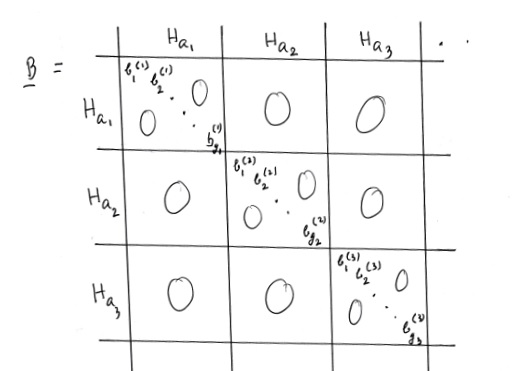
\includegraphics[scale=1.0]{C.jpg}
\vspace{-6 mm}
\caption{The matrix representation of $\hat{B}$ in the eigenbasis consisting of simultaneous eigenvectors of
$\hat{A}$ and $\hat{B}$.}
\label{fig:C}
\end{figure}



\paragraph{}
The diagonal entries $b_i^{(n)}, i=1,2, \cdots , g_n$ in each eigensubspace $H_{a_n}$ in figure (\ref{fig:C}) are the various eigenvalues of the operator $\hat{B}$, i.e., $b_i^{(n)} \in \{b_1,b_2, \cdots\}$. In a given eigensubspace $H_{a_n}$, some of the eigenvalues of
$\hat{B}$ may be repeated. Further, a particular eigenvalue of $\hat{B}$ may also be repeated in several eigensubspaces $H_{a_n}$.

\paragraph{}
Thus, in summary, what we have shown is that, given two Hermitian operators $\hat{A}$ and $\hat{B}$ representing
two observables of a quantum system,  it is possible to construct a complete set of simultaneous eigenvectors 
spanning the entire Hilbert space provided  $[\hat{A},\hat{B}]=0$. Hence, we have proved that $[\hat{A},\hat{B}]=0$ is a sufficient condition for two Hermitian operators $\hat{A}$ and $\hat{B}$ to be compatible.


% New section
% Sec 5
\section{Labeling of Quantum Mechanical Basis States}
Since eigenvectors of a Hermitian operator corresponding to an observable form a complete set, we can label the members of the set by the eigenvalues. Thus, suppose that an observable $\hat{A}$ has eigenvalues
\[ a_1, a_2, a_3, \cdots\, . \]
The basis states are then labeled as
\[ |a_1\rangle,\, |a_2\rangle,\, |a_3\rangle,\, \cdots \, . \]
The labeling would be unambiguous if the eigenvalues were all non-degenerate. However, if some or all eigenvalues are degenerate, we will need another mark of distinction for the eigenvectors. 

\paragraph{}
For example, if an eigenvalue $a_n$ is $g_n$-fold degenerate, the corresponding eigenvectors may be denoted as
\[ |a_n,i\rangle,\, i=1,2, \cdots , g_n\, . \]
An alternative, and better, notation is based on the fact that two compatible observables whose Hermitian operators commute, may be assumed to have the same set of eigenvectors. Hence, if we can find a second observable $\hat{B}$ commuting with the first, such that
\be
\hat{B}|a_n,i\rangle = b_i|a_n,i\rangle,\, i=1,2, \cdots , g_n 
\ee
with eigenvalues $b_i$ all different, then the eigenvalues of $\hat{B}$ may serve to distinguish the eigenvectors.
So, we can write
\[
\begin{array}{lcl}
|a_n,1\rangle & \equiv & |a_n,b_1\rangle \\
|a_n,2\rangle & \equiv & |a_n,b_2\rangle \\
. & & . \\
. & & . \\
. & & . \\
|a_n,g_n\rangle & \equiv & |a_n,b_{g_n}\rangle\, . 
\end{array}
\]
But, if some of the eigenvalues $b_i, i=1,2, \cdots, g_n$ are equal, we will need a third mark to distinguish the eigenvectors. The third mark may be obtained if we can find a third observable whose operator $\hat{C}$ commutes with both $\hat{A}$ and 
$\hat{B}$. Then $\hat{A}$, $\hat{B}$ and $\hat{C}$ have simultaneous eigenvectors and the eigenvalues of $\hat{C}$ may also be used to label the eigenvectors.

\paragraph{}
Thus, in general, if we can find a set of mutually commuting Hermitian operators, $\hat{A},\hat{B},\hat{C},\hat{D} , \cdots $
whose common eigenvectors can be characterized completely by the eigenvalues $a,b,c,d, \cdots$ such that no two eigenvectors have exactly identical set of eigenvalues, then the eigenvalues of these operators can uniquely label the common eigenvectors.
Such a set of Hermitian operators is said to be complete. We refer to this set of operators as a complete set of commuting 
observables (CSCO). 

\paragraph{}
In the new notation, the basis vectors are written as
\[ |a,b,c, d, \, \cdots \rangle \, . \]
The normalization and completeness conditions are then 
\be
\langle a^{\prime},b^{\prime},c^{\prime}, d^{\prime} \cdots |a,b,c,d,\cdots \rangle = \delta_{aa'}\delta_{bb'} \cdots \, ,
\ee
and
\be
\sum_{(a,b,c,d,\cdots)} |a,b,c,d,\cdots \rangle \langle a,b,c,d,\cdots |= \hat{I} \, . 
\ee










\include{Chapter9/chapter9}
\chapter{sheet-10 : Harmonic Oscillator}

From the Hamiltonian find the operators by making the Hamiltonian dimensionless first. QM lecture MIT 2013 by Allan Adams.

\include{Chapter11/chapter11}
%% writing by shahnoor


\chapter{sheet-12 : The Path Integral Formulation of Quantum Theory}

\ifpdf
\graphicspath{{Chapter12/figs/}}
\else
\graphicspath{{Chapter12/figs/}}
\fi


\section{Background Materials}
\begin{enumerate}
	\item Basis states
	\begin{align}
		\hat{Q}_s \ket{q} &= q\ket{q} \\
		\hat{P}_s \ket{p} &= p\ket{p} 
	\end{align}
	The states $\{\ket{q}\}$ and $\{\ket{p}\}$ are basis states, i.e., $\mathbbm{1}$
	\begin{align}
		\int \dd{q} \ket{q}\bra{q} &= \mathbb{1} \\
		\int \dd{p} \ket{p}\bra{p} &= \mathbb{\hat{1}} \\
	\end{align}
	where the normalization is chosen as
	\begin{align}
		\braket{q}{q^\prime} &= \delta(q-q^\prime) \\
		\braket{p}{p^\prime} &= \delta(p-p^\prime) 
	\end{align}
	The operators $\hat{Q}_s$ and $\hat{P}_s$ can be expressed in coordinate representation as follows
	\begin{align}
		\bra{q}\hat{Q}_s &= q \bra{q} \\
		\bra{q}\hat{P}_s &= -\iu \hbar \pdv{q} \bra{q} 
	\end{align}
	In momentum representaion
	\begin{align}
		\bra{p}\hat{Q}_s &= \iu \hbar \pdv{p} \bra{p} \\
		\bra{p}\hat{P}_s &=  \bra{p} 
	\end{align}
	The fundamental commutation relation between $\hat{Q}$ and $\hat{P}$ is 
	\begin{equation}
		\left[\hat{Q}_s, \hat{P}_s\right] = \iu
		 \hbar \mathbb{\hat{1}}
	\end{equation}
	For later purposes we will need the momentum eigenstates in coordinate representation, i.e., $\braket{q}{p}$. To find $\braket{q}{p}$ we proceed as follows
	\begin{align}
		\hat{P}_s \ket{p} &= p\ket{p} \\
		\bra{q}\hat{P}_s \ket{p} &= p\bra{q}\ket{p} \\
		-\iu \hbar \pdv{q} \braket{q}{p} &= p \braket{q}{p}
	\end{align}
	This equation is easy to solve for $\braket{q}{p}$. We find
	\begin{equation}
		\braket{q}{p} = C e^{\iu p q / \hbar}
	\end{equation}
	The constant $C$ is chosen such that we have the normalization $\braket{p}{p^\prime } \delta(p-p^\prime)$. Now
	\begin{align*}
		\braket{p}{p^\prime} 
		&= \int \dd{q} \braket{p}{q}\braket{q}{p^\prime} \\
		&= \int \dd{q} C^* e^{-ipq/\hbar} C^{\iu p^\prime q /\hbar} \\
		&= \left|C\right|^2 \int_{-\infty}^{\infty} \dd{q} e^{-\iu(p-p^\prime)q/\hbar} \\
		&= \left|C\right|^2  2\pi \delta(\frac{p-p^\prime}{\hbar}) \\
		&= \left|C\right|^2  2\pi \hbar \delta(p-p^\prime)
	\end{align*}
	Choosing $C$ to be real and positive, we must have
	\begin{equation}
		C = \frac{1}{\sqrt{2\pi \hbar}}
	\end{equation}
	Thus
	\begin{equation}
		\braket{q}{p} = \frac{1}{\sqrt{2\pi \hbar}} e^{\iu p q / \hbar}
	\end{equation}
	
	
	\item Quantum Mechanics in Heisenberg picture//
	The Heisenberg picture of quantum dynamics is obtained from the Schr\"{o}dinger picture by the following transformation of all kets and all operators
	\begin{align}
		\ket{}_H &= e^{\iu \hat{H}t/\hbar}\ket{}_s \label{chapter12.eqn-schrodinger-to-heisengerg-ket}\\
		\hat{\Omega}_H(t) &= e^{\iu \hat{H}t/\hbar} \hat{\Omega}_S e^{-\iu \hat{H}t/\hbar}
		\label{chapter12.eqn-schrodinger-to-heisengerg-operator}
	\end{align}
	where we have assumed the system is conservative, i.e., $\hat{H}$ is independent of time. 
	
	In the Heisenberg picture, the base kets, for example, the eigenkets of $\hat{Q}_H(t)$ and $\hat{P}_H(t)$ are time dependent. We have
	\begin{align}
		\hat{Q}_H(t) \ket{q,t}_H &= q \ket{q,t}_H \\
		\hat{P}_H(t) \ket{p,t}_H &= p \ket{p,t}_H
	\end{align}
	where
	\begin{align}
		\ket{q,t}_H &= e^{\iu \hat{H}t/\hbar}\ket{q}\\
		\ket{p,t}_H &= e^{\iu \hat{H}t/\hbar}\ket{p}
	\end{align}
	and
	\begin{align}
		\hat{Q}_H(t) &= e^{\iu \hat{H}t/\hbar} \hat{Q}_S e^{-\iu \hat{H}t/\hbar}\\
		\hat{P}_H(t) &= e^{\iu \hat{H}t/\hbar} \hat{P}_S e^{-\iu \hat{H}t/\hbar}
	\end{align}
	The orthogonality and completeness of the Heisenberg picture base kets are
	\begin{align}
		_H\braket{q,t}{q^\prime,t}_H = \braket{q}{q^\prime} &=  \delta(q-q^\prime) \\
		_H\braket{p,t}{p^\prime,t}_H = \braket{p}{p^\prime} &=  \delta(p-p^\prime) 
	\end{align}
	Note that these are equal time relations. And
	\begin{align}
		\hat{\mathbb{1}} &= \int \dd{q} \ket{q,t}_H \  {_H}\bra{q,t}\label{chapter12.eqn1-completeness-q}\\
		\hat{\mathbb{1}} &= \int \dd{p} \ket{p,t}_H\ {_H}\bra{p,t}\label{chapter12.eqn1-completeness-p}
	\end{align}
	To show the validity of equation (\ref{chapter12.eqn1-completeness-q}), for example, we use the transformation of kets and bras from the schr\"{o}dinger picture to the Heisenberg picture (\ref{chapter12.eqn-schrodinger-to-heisengerg-ket}), i.e., 
	\begin{equation}
		{_H}\bra{} = {_S}\bra{} e^{-\iu \hat{H}t/\hbar} 
	\end{equation}
	Thus the right hand side of equation (\ref{chapter12.eqn1-completeness-q}) can be written as
	\begin{align}
		\int \dd{q}  \ket{q,t}_H {_H}\bra{q,t} &= \int \dd{q} \quad e^{\iu \hat{H}t/\hbar}\ket{q} \bra{q}e^{-\iu \hat{H}t/\hbar} \\
		&= e^{\iu \hat{H}t/\hbar}\left(\int \dd{q}  \ket{q} \bra{q}\right)e^{-\iu \hat{H}t/\hbar} \\
		&= e^{\iu \hat{H}t/\hbar}\quad\mathbb{1}\quad e^{-\iu \hat{H}t/\hbar} \\
		&= \mathbb{1}
	\end{align}
	We note that the \underline{state vector} in the Heisenberg picture is independent of time, while the state vector in the Schr\"{o}dinger picture is time-dependent. This is very simply shown as follows:
	\begin{align}
		\ket{\psi}_H &= e^{\iu \hat{H}t/\hbar} \ket{\psi(t)}_S \\
		&= e^{\iu \hat{H}t/\hbar} e^{-\iu \hat{H}t/\hbar} \ket{\psi(0)}_S\\
		&= \ket{\psi(0)}_S
	\end{align}
	Thus the state ket in the Heisenberg picture is independent of time and is same as the initial state ket in the Schr\"{o}dinger picture.
	
	\end{enumerate}


	\section{Propagator}
	The dynamics of a quantum system is completely specified by the "Feynman Kernel", or the propagator or the transition amplitude defined as
	%%%%%%%%%%%%%
	%%%%%%%%%% TODO
	%%%%%%%%%%%%%
	\begin{equation}
		U(q_2, t_2; q_1, t_1) =
		\tensor[_H]{\braket{q_2, t_2}{q_1, t_1}}{_H}
		\label{chapter12.eqn1-propagator}
	\end{equation}
	Transforming to the Schr\"{o}dinger picture base kets, we can write equation (\ref{chapter12.eqn1-propagator}) as
	\begin{align}
		U(q_2, t_2; q_1, t_2) 
		&= \bra{q_2}e^{-\iu \hat{H}t_2/\hbar} e^{\iu \hat{H}t_1/\hbar} \ket{q_1} \nonumber \\
		&= \bra{q_2}e^{-\iu \hat{H}(t_2-t_1)/\hbar} \ket{q_1} \label{chapter12.eqn2-propagator}
	\end{align}
	We see that the propagator is the matrix element in the coordinate basis of the time-evolution operator in the Schr\"{o}dinger picture. The physical meaning of the propagator is that it is the probability amplitude of finding the particle at $q_2$ at time $t_2$ if the particle was at $q_1$ at an earlier time $t_1$. Knowing the propagator is equivalent to solving the Schr\"{o}dinger equation, for it allows us to calculate the Schr\"{o}dinger picture wave function at any moment of time if the wave function is known at an earlier moment. This is shown below:
	\begin{align}
		\psi_S(q,t )
		&= \braket{q}{\psi_S(t)} \\
		&= \bra{q}e^{-\iu \hat{H}t/\hbar} \ket{\psi_S(0)} \\
		&= \tensor[_H]{\braket{q,t}{\psi}}{_H} \\
		&= \int \dd{q^\prime} \tensor[_H]{\braket{q,t}{q^\prime, t^\prime}}{_H} \tensor[_H]{\braket{q^\prime, t^\prime}{\psi}}{_H} \\
		&= \int \dd{q^\prime} U(q,t;q^\prime, t^\prime) \psi_S(q^\prime,t^\prime)
	\end{align}
	The path integral formalism of quantum dynamics provides a means to construct the transition amplitude $\tensor[_H]{\braket{q,t}{q^\prime, t^\prime}}{_H}$ from the classical Hamiltonian or Lagrangian alone, without any reference to non commuting operators or Hilbert space vectors.

	\section{Path Integral for the Propagator}
		We will now calculate
		\begin{equation}
			U(x,t;x_0, t_0) = \tensor[_H]{\braket{x,t}{x_0, t_0}}{_H}
			\label{chapter12.eqn1-propagator-path-integral}
		\end{equation}
		where $t>t_0$. For this purpose let us devide the time integral $(t,t_0)$ into $N$ equal segments each of duration $\epsilon$. Namely, let
		\begin{equation}
			\epsilon = \frac{t-t_0}{N}
			\label{chapter12.eqn2-propagator-path-integral}
		\end{equation}
		In other words, we are discretizing the time interval, and in the end we will take the continuum limit $\epsilon\rightarrow 0$ and $N\rightarrow \infty$. We label the end times $t_0$ and $t$ and the intermediate times as $t_1, t_2, \ldots, t_{N-1}, t_N=t$. Further, we will let $x_N=x$. The intermediate times are 
		\begin{equation}
			t_i=t_0+i \epsilon, \quad i=1,2,\ldots,N-1
			\label{chapter12.eqn3-propagator-path-integral}
		\end{equation}
		
		At each intermediate time a complete set of basis states $\ket{x_i,t_i}$ may be inserted:
		\begin{equation}
			\braket{x t}{x_0 t_0} =\int_{-\infty}^{\infty}\dd{x_1} \ldots \int_{-\infty}^{\infty} \dd{x_{N-1}} \braket{x t}{x_{N-1} t_{N-1}}\braket{x_{N-1} t_{N-1}}{x_{N-2} t_{N-2}} \ldots \braket{x_2 t_2}{x_{1} t_{1}} \braket{x_1 t_1}{x_{0} t_{0}}
			\label{chapter12.eqn4-propagator-path-integral}
		\end{equation}
		
		Here we have omitted the subscript $H$ in the Heisenberg picture basis vectors since there is no scope for confusion. Note that while there are $N$ scalar products in euquation (\ref{chapter12.eqn4-propagator-path-integral}), there are only $N-1$ intermediate points so that the number of integrations is $N-1$. Since $x_N = x$ and $t_N= t$, we can write equation (\ref{chapter12.eqn4-propagator-path-integral}) as
		\begin{equation}
			\braket{x t}{x_0 t_0} = \int \prod_{i=1}^{N-1} \dd{x_i} \prod_{i=0}^{N-1} \braket{x_{i+1} t_{i+1}}{x_i t_i}
			\label{chapter12.eqn5-propagator-path-integral}
		\end{equation}
		Equation (\ref{chapter12.eqn5-propagator-path-integral}) can be interpreted as follows: A particle that propagates from $x_0$ at time $t_0$ to $x$ at time $t$ can take an arbitrary intermediate trajectory, shown in figure (\ref{chapter12.fig1-propagator-path-integral-trajectory})
		\begin{figure}
			\centering
			
\includegraphics[width=0.5\linewidth]{Pictures/not-found.jpg}
			\caption{text}
			\label{chapter12.fig1-propagator-path-integral-trajectory}
		\end{figure}
	
	Such a path is characterized by the coordinate values $x_i$ at intermediate grid points in the time interval $(t_0,t)$. One such path is shown in the figure as a zigzag curve. Since each intermediate coordinates $x_i\quad (i=1,2,\ldots,N-1)$ can vary form $-\infty$ to $\infty$, it is essential that all conceivable paths connecting the end points are taken into account. According tot the representation principle of Quantum Mechanics they all contribute to the transition amplitude (\ref{chapter12.eqn5-propagator-path-integral}). Of course, some trajectories may turn out to be more important than others.
	
	
	We will now calculate the intermediate scalar products which themselves are propagators but over infinitesimal time intervals. An intermediate scalar product has the form $\braket{x_{i+1} t_{i+1}}{x_i t_i}$. We can calculate this inner product up to first order in $\epsilon$ from equation (\ref{chapter12.eqn2-propagator-path-integral}) as follows
	\begin{align}
		\braket{x_{i+1} t_{i+1}}{x_i t_i} &= \bra{x_{i+1}} e^{-\iu \hat{H}t_{i+1}/\hbar}e^{\iu \hat{H}t_{i}/\hbar}\ket{x_i}\\
		&= \bra{x_{i+1}} e^{-\iu \hat{H}(t_{i+1} - t_i)/\hbar}\ket{x_i}\\
		&= \bra{x_{i+1}} e^{-\iu \hat{H}\epsilon/\hbar}\ket{x_i}\\
		&= \bra{x_{i+1}} \left(\mathbb{1} - \frac{\iu \epsilon}{\hbar}\hat{H} + \order{\epsilon^2}\right)\ket{x_i}
	\end{align}
	We will take $\hat{H}$ to be of the form
	\begin{equation}
		\hat{H} = \frac{\hat{P}}{2 m} + V(\hat{X})
	\end{equation}
	Therefore
	\begin{align}
		\braket{x_{i+1} t_{i+1}}{x_i t_i} 
		&= \bra{x_{i+1}}\left[\mathbb{1} - \frac{\iu \epsilon}{\hbar}\left(\frac{\hat{P}^2}{2 m} + V(\hat{X}) + \right) + \order{\epsilon^2}\right]\ket{x_i}\\
		&= \int_{-\infty}^{\infty} \dd{p} \braket{x_{i+1}}{p} \bra{p} \left[\mathbb{1} - \frac{\iu \epsilon}{\hbar}\left(\frac{\hat{P}^2}{2 m} + V(\hat{X})\right) + \order{\epsilon^2}\right] \ket{x_i} \\
		&= \int_{-\infty}^{\infty} \dd{p} \braket{x_{i+1}}{p} \braket{p}{x_i} \left[\mathbb{1} - \frac{\iu \epsilon}{\hbar}\left(\frac{p^2}{2 m} + V(x_i)\right) + \order{\epsilon^2}\right]  \\
		&= \int \dd{p} \frac{1}{\sqrt{2\pi \hbar}}e^{\iu p x_{i+1}/\hbar}\frac{1}{\sqrt{2\pi \hbar}}e^{-\iu p x_{i}/\hbar} e^{-\iu \epsilon/\hbar \left( \frac{p^2}{2 m} + V(x_i) \right)} \\
		&= \frac{1}{2\pi\hbar} \int_{-\infty}^{\infty} \dd{p} e^{\iu p (x_{i+1} - x_i)/\hbar} e^{-\iu \epsilon/\hbar \left( \frac{p^2}{2 m} + V(x_i) \right)} \\
		&= \frac{1}{2\pi\hbar} e^{-\iu \epsilon V(x_i)/\hbar} \int_{-\infty}^{\infty} e^{\iu p \epsilon\frac{(x_{i+1} - x_i)}{\epsilon}\frac{1}{\hbar}} e^{-\iu \epsilon/\hbar \left( \frac{p^2}{2 m}\right)} \dd{p}\\
		&= \frac{1}{2\pi\hbar} e^{-\iu \epsilon V(x_i)/\hbar} \int_{-\infty}^{\infty} e^{\iu p \epsilon \dot{x}_i / \hbar} e^{-\iu \epsilon \frac{p^2}{2 m \hbar}} \dd{p} \\
		&= \frac{1}{2\pi\hbar} e^{-\iu \epsilon V(x_i)/\hbar} \int_{-\infty}^{\infty} e^{-\frac{\iu \epsilon}{2 m \hbar} \left(p^2 - 2 m p \dot{x}_i \right)} \dd{p}
		\label{chapter12.eqn6-path-integral-propagator}
	\end{align}
	In the above we have defined
	\begin{equation}
		\dot{x}_i = \frac{x_{i+1} - x_i}{\epsilon}
	\end{equation}
	Now
	\begin{equation}
		p^2 - 2m p \dot{x}_i = (p- m \dot{x}_i)^2 - m^2 \dot{x}_i^2
	\end{equation}
	We make the change of variable
	\begin{equation}
		p^\prime = p -m \dot{x}_i
	\end{equation}
	Therefore equation (\ref{chapter12.eqn6-path-integral-propagator}) can be written as
	
	\begin{align}
		\braket{x_{i+1} t_{i+1}}{x_i t_i} 
		&= \frac{1}{2 \pi \hbar} e^{-\iu \epsilon V(x_i)/\hbar} e^{-\iu \epsilon (-m^2 \dot{x}_i^2) / 2 m \hbar}  \int_{-\infty}^{\infty} \dd{p^\prime} e^{-\iu \epsilon {p^\prime}^2 / 2 m \hbar} \\
		&= \frac{1}{2 \pi \hbar} e^{\frac{\iu \epsilon}{\hbar} \left(\frac{1}{2} m \dot{x}_i^2 - V(x_i)\right)} \int_{-\infty}^{\infty} \dd{p^\prime} e^{-\iu \epsilon {p^\prime}^2 / 2 m \hbar}
	\end{align}
	Now we use the standard integral
	\begin{equation}
		\int_{-\infty}^{\infty} e^{-\alpha x^2} \dd{x} = \sqrt{\frac{\pi}{\alpha}}
	\end{equation}
	to get
	\begin{equation}
		\int_{-\infty}^{\infty} \dd{p^\prime} e^{-\iu \epsilon p^\prime / 2 m \hbar} = \left(\frac{\pi}{\iu \epsilon/2 m \hbar}\right)^{1/2} = \left(\frac{2 \pi \hbar m}{\iu \epsilon}\right)^{1/2}
	\end{equation}
	Therefore
	\begin{align}
		\braket{x_{i+1} t_{i+1}}{x_i t_i} 
		&= \frac{1}{2 \pi \hbar} \left(\frac{2 \pi \hbar m}{\iu \epsilon}\right)^{1/2} e^{\frac{\iu \epsilon}{\hbar} \left(\frac{1}{2} m \dot{x}_i^2 - V(x_i)\right)} \\
		&= \left(\frac{m}{2\pi\hbar\iu \epsilon}\right)^{1/2} e^{\frac{\iu \epsilon}{\hbar} \left(\frac{1}{2} m \dot{x}_i^2 - V(x_i)\right)}
		\label{chapter12.eqn7-path-integral-propagator}
	\end{align}
	We now substitute equation (\ref{chapter12.eqn7-path-integral-propagator}) into equation (\ref{chapter12.eqn5-propagator-path-integral}) to get
	\begin{align}
		\braket{x t}{x_0 t_0} 
		&= \int \prod_{i=1}^{N-1} \dd{x_i} \prod_{i=0}^{N-1} \braket{x_{i+1} t_{i+1}}{x_i t_i}\\
		&= \int \prod_{i=1}^{N-1} \dd{x_i} \prod_{i=0}^{N-1} \left(\frac{m}{2 \pi \hbar \iu \epsilon}\right)^{1/2} e^{\frac{\iu \epsilon}{\hbar} \left(\frac{1}{2} m \dot{x}_i^2 - V(x_i)\right)} \\
		&= \left(\frac{m}{2 \pi \hbar \iu \epsilon}\right)^{N/2} \int \prod_{i=1}^{N-1} \dd{x_i}e^{\frac{\iu}{\hbar} \sum_{i=0}^{N-1} \epsilon \left(\frac{1}{2} m \dot{x}_i^2 - V(x_i)\right)}
		\label{chapter12.eqn8-path-integral-propagator}
	\end{align}
	We now consider a path $x(t^\prime)$ connecting the initial and the final space-time point such that the value of $x(t^\prime)$ at the intermediate times $t_1, t_2, \ldots, t_{N-1}$ are $x(t_i^\prime)=x_i$. Therefore we can write
	\begin{align}
		\sum_{i=0}^{N-1} \epsilon \left(\frac{1}{2} m \dot{x}_i^2 - V(x_i)\right) 
		&= \int_{t_0}^{t} \left[\frac{1}{2} m \dot{x}^2(t^\prime) - V(x(t^\prime))\right] \dd{t^\prime} \\
		&= \int_{t_0}^{t} L\left(x(t^\prime), \dot{x}(t^\prime)\right) \dd{t^\prime} \\
		&= S[x(t^\prime)]
	\end{align}
	Where $S\left[x(t^\prime)\right]$ is the action calculated along the particular path. Since we are integrating over $x_i\quad (i=1,\ldots,N-1)$, we are effectively summing the exponential in equation (\ref{chapter12.eqn8-path-integral-propagator}) over all conceivable paths connecting $(x_0, t_0)$ to $(x, t)$. We define the path integral as
	\begin{equation}
		\mathcal{D}[x(t^\prime)] = \lim\limits_{N\rightarrow \infty} \left(\frac{m}{2 \pi \hbar \iu \epsilon}\right)^{N/2} \int \prod_{i=1}^{N-1} \dd{x_i}
		\label{chapter12.eqn9-path-integral-propagator}
	\end{equation}
	Therefore, we can write equation (\ref{chapter12.eqn8-path-integral-propagator}) as
	\begin{equation}
		\braket{x, t}{x_0, t_0} = \int \mathcal{D}\left[x(t^\prime)\right] e^{\frac{i}{\hbar} S\left[x(t^\prime)\right]}
		\label{chapter12.eqn10-path-integral-propagator}
	\end{equation}
	This is the path integral formula for the propagator. We can think of equation (\ref{chapter12.eqn10-path-integral-propagator}) as a sysbolic way of writing equation (\ref{chapter12.eqn8-path-integral-propagator}) with $N \rightarrow \infty$. In calculating path integrals we use equation (\ref{chapter12.eqn8-path-integral-propagator}) and set $N \rightarrow \infty$.
	
	\section{Path Integral for a Free Particle}
	For a free particle $V=0$. Therefore the lagrangian is
	\begin{equation}
		L = T - V = T = \frac{1}{2} m \dot{x}^2(t)
		\label{chapter12.eqn11-path-integral-free-particle}
	\end{equation}
	the path integral formula for the propagator of a free particle is
	\begin{align}
		\braket{x, t}{x_0, t_0} 
		&= \int \mathcal{D}\left[x(t^\prime)\right] \exp\left[\frac{\iu}{\hbar} S\left[x(t^\prime)\right]\right] \\
		&= \lim\limits_{N \rightarrow \infty} \left(\frac{m}{2 \pi \hbar \iu \epsilon}\right)^{N/2} \int \prod_{i=1}^{N-1} \dd{x_i} \exp\left[\frac{\iu \epsilon}{\hbar} \sum_{i=0}^{N-1} \frac{1}{2} m \dot{x}_i^2\right]
		\label{chapter12.eqn12-path-integral-free-particle}
	\end{align}
	In equation (\ref{chapter12.eqn12-path-integral-free-particle})
	\begin{equation}
		\epsilon = \frac{t - t_0}{N}
	\end{equation}
	Also $\dot{x}_i$ can be written as
	\begin{equation}
		\dot{x}_i = \frac{x_{i+1} - x_i}{\epsilon}
		\label{chapter12.eqn13-path-integral-free-particle}
	\end{equation}
	
	\begin{figure}
		\centering
		
\includegraphics[width=0.5\linewidth]{Pictures/not-found.jpg}
		\caption{text}
		\label{chapter12.fig2}
	\end{figure}
	For notational convenience we let $x_N = x$ where $x$ is the final position. We only integrate over the position the particle may have at intermediate times $t_1, t_2, \ldots, t_{N-1}$.
	
	Using equation (\ref{chapter12.eqn13-path-integral-free-particle}), equation (\ref{chapter12.eqn12-path-integral-free-particle}) can be written as
	\begin{align}
		\braket{x t}{x_0 t_0} 
		&= \lim\limits_{N \rightarrow \infty} \left(\frac{m}{2\pi \hbar \iu \epsilon}\right)^{N/2} \int \prod_{i=1}^{N-1} \dd{x_i} e^{\frac{\iu \epsilon}{\hbar} \sum_{i=0}^{N-1} \frac{m}{2} \left(\frac{x_{i+1} - x_i}{\epsilon}\right)^2} \\
		&= \lim\limits_{N \rightarrow \infty} \left(\frac{m}{2\pi \hbar \iu \epsilon}\right)^{N/2} \int \prod_{i=1}^{N-1} \dd{x_i} e^{\frac{\iu m}{2\hbar \epsilon} \sum_{i=0}^{N-1} (x_{i+1} - x_i)^2}
		\label{chapter12.eqn14-path-integral-free-particle}
	\end{align}
	At this stage it is convenient to make a change of variable
	\begin{equation}
		y_i = \left(\frac{m}{2\hbar \epsilon}\right)^{1/2} x_i
	\end{equation}
	In terms of new variables equation (\ref{chapter12.eqn14-path-integral-free-particle}) is written as
	\begin{equation}
		\braket{x t}{x_0 t_0} 
		= \lim\limits_{N \rightarrow \infty} \left(\frac{m}{2\pi \hbar \iu \epsilon}\right)^{N/2} \left(\frac{2\hbar \epsilon}{m}\right)^{(N-1)/2} \int \prod_{i=1}^{N-1} \dd{y_i} e^{-\sum_{i=0}^{N-1} \frac{(y_{i+1} - y_i)^2}{i}}
		\label{chapter12.eqn15-path-integral-free-particle}
	\end{equation}
	We now have to do the gaussian integral over the variables $y_1, y_2, \ldots, y_{N-1}$.
	
	\textbf{$y_1$ integral}
	Take $N=2$ in Eq. (\ref{chapter12.eqn15-path-integral-free-particle})
	\begin{equation}
		I_1 = \int_{-\infty}^{\infty} \dd{y_1} \exp\left[-\frac{1}{\iu} \left[(y_1 - y_0)^2 + (y_2 - y_1)^2\right]\right]
	\end{equation}
	consider the exponent
	\begin{equation}
		(y_1 - y_0)^2 + (y_2 - y_1)^2 = 2 y_1^2 - 2 (y_0 + y_2) y_1 + (y_0^2+y_2^2)
	\end{equation}
	therefore,
	\begin{equation}
		I_1 = \exp \left[-\frac{1}{\iu} \left(y_0^2+ y_2^2\right)\right] \int_{-\infty}^{\infty} \dd{y_1} \exp\left[-\frac{1}{\iu} \left(2y_1^2 - 2(y_0 + y_2) y_1\right)
		\right]
	\end{equation}
	Now we use the standard integral
	\begin{equation}
		\int_{-\infty}^{\infty} e^{-\alpha x^2 + \beta x} \dd{x} = \left(\frac{\pi}{\alpha}\right)^{1/2} \exp \left(\frac{\beta^2}{4\alpha}\right)
	\end{equation}
	choosing $\alpha = \frac{2}{\iu}$ and $\beta = \frac{2(y_0 + y_2)}{\iu}$
	\begin{align*}
		I_1 
		&= \exp \left[-\frac{1}{\iu} (y_0^2 + y_2^2)\right] \left(\frac{\iu \pi}{2}\right)^{1/2} \exp\left[\frac{-4 \left(y_0 +y_2\right)^2}{4 (2/\iu)}\right]\\
		&= \exp \left[-\frac{1}{\iu} (y_0^2 + y_2^2)\right] \left(\frac{\iu \pi}{2}\right)^{1/2} \exp\left[\frac{\left(y_0 +y_2\right)^2}{2\iu}\right] \\
		&= \left(\frac{\iu \pi}{2}\right)^{1/2} \exp \left[-\frac{1}{2\iu} \left( 2(y_0^2 + y_2^2) - \left(y_0 +y_2\right)^2 \right)\right]
	\end{align*}
	Thus
	\begin{equation}
		I_1 = \left(\frac{\iu \pi}{2}\right)^{1/2} \exp \left[-\frac{1}{2\iu} \left(y_2 - y_0\right)^2\right]
		\label{chapter12.eqn16-path-integral-free-particle}
	\end{equation}
	Next we do the integral over $y_2$. The variable $y_2$ occurs in the $i=2$ term in equation (\ref{chapter12.eqn15-path-integral-free-particle}) and also in $I_1$ in Eq. (\ref{chapter12.eqn16-path-integral-free-particle}). Thus taking $N=3$ in Eq. (\ref{chapter12.eqn15-path-integral-free-particle})
	
	\begin{align*}
	I_2 &= \int \dd{y_1} \dd{y_2} \exp[-\frac{1}{\iu}\qty[\qty(y_1 - y_0)^2 + \qty(y_2 - y_1)^2 + \qty(y_3 - y_2)^2]] \\
	&=\int \dd{y_2} \exp \left[-\frac{1}{\iu} \left(y_3 - y_2\right)^2\right] I_1
	\end{align*}
	
	Therefore, the $y_2$ integral is
	\begin{align*}
		I_2 
		&= \int \dd{y_2} \exp \left[-\frac{1}{\iu} \left(y_3 - y_2\right)^2\right] \left(\frac{\iu \pi}{2}\right)^{1/2} \exp \left[-\frac{1}{2 \iu} \left(y_2 - y_0\right)^2\right] \\
		&= \left(\frac{\iu \pi}{2}\right)^{1/2} \int \dd{y_2} \exp \left[-\frac{1}{\iu} \left(y_3 - y_2\right)^2 -\frac{1}{2 \iu} \left(y_2 - y_0\right)^2\right] \\
		&= \left(\frac{\iu \pi}{2}\right)^{1/2} \int \dd{y_2} \exp \left[-\frac{1}{2\iu} \{2 \left(y_3 - y_2\right)^2 + \left(y_2 - y_0\right)^2\}\right] \\
	\end{align*}
	Consider the term in the curly brackets
	\begin{align*}
		2\left(y_3 - y_2\right)^2 + \left(y_2 - y_0\right)^2 &= 2\left(y_3^2 + y_2^2 - 2y_2 y_3\right) + \left(y_2^2 + y_0^2 - 2 y_0 y_2\right) \\
		&= 3 y_2^2 - 2y_2 \left(2y_3 + y_0\right) + \left(2 y_3^2 + y_0^2\right)
	\end{align*}
	where the first term is quadratic in $y_2$, second term is linear in $y_2$ and the last term is independent of $y_2$. We have
	\begin{equation}
		I_2 = \left(\frac{\iu \pi}{2}\right)^{1/2} \exp\left[-\frac{1}{2\iu}\left(2 y_3^2 + y_0^2\right)\right] \int \dd{y_2} \exp\left[-\frac{1}{2\iu} \left(3 y_2^2 - 2y_2 \left(2 y_3 + y_0\right)\right) \right]
	\end{equation}
	
	We use standard integral (\ref{appendix1.eqn2}) from appendix (\ref{appendix1.Integrals}) and choose
	\begin{align}
		\alpha &= \frac{3}{2\iu} \\
		\beta &= \frac{\left(y_0 2 y_3\right)}{\iu}
	\end{align}
	
	\begin{align*}
		I_2 
		&= \left(\frac{\iu \pi}{2}\right)^{1/2} \exp\left[-\frac{1}{2\iu} \left(2 y_3^2 + y_0^2\right)\right] \left(\frac{2\pi \iu}{3}\right)^{1/2} \exp\left[-\frac{\left(y_0 + 2 y_3\right)^2}{6/\iu}\right] \\
		&= \left(\frac{\iu \pi}{2}\right)^{1/2} \left(\frac{2\pi \iu}{3}\right)^{1/2}  \exp\left[-\frac{1}{2\iu} \left(2 y_3^2 + y_0^2\right)\right]  \exp\left[\frac{\left(y_0 + 2 y_3\right)^2}{6\iu}\right] \\
		&= \qty(\frac{\iu^2 \pi^2}{3})^{1/2} \exp\left[-\frac{1}{\iu}\qty{\frac{1}{3} y_3^2 + \frac{1}{3} y_0^2 -\frac{2}{3} y_0 y_3}\right]
	\end{align*}
	\begin{equation}
		I_2 = \qty(\frac{\iu^2 \pi^2}{3})^{1/2} \exp\left[-\frac{(y_3-y_0)^2}{3\iu}\right]
		\label{chapter12.eqn17-path-integral-free-particle}
	\end{equation}
	Now the trend is clear. Finally, integrating $(N-1)$ times we get
	\begin{equation}
		I_{N-1} = \frac{\left(\iu \pi\right)^{(N-1)/2}}{N^{1/2}} \exp\left[-\left(y_N - y_0\right)^2/N\iu
		\right]
	\end{equation}
	where $y_N = y$.

	Therefore, the path integral formula for the propagator of a free particle is (using the above formula in equation (\ref{chapter12.eqn15-path-integral-free-particle}))
	\begin{align}
		\braket{x t}{x_0 t_0}_{free} &= U_{free}\left(x, t; x_0, t_0\right) \nonumber\\
		&= \lim\limits_{N\rightarrow \infty} \left(\frac{m}{2\pi \hbar \iu \epsilon}\right)^{N/2} \left(\frac{2\hbar\epsilon}{m}\right)^{(N-1)/2}  \frac{(\iu \pi)^{(N-1)/2}}{N^{1/2}} \exp\left[-\left(y_N - y_0\right)^2 / N\iu
		\right]
	\end{align}
	previously we defined
	\begin{equation}
		y = \left(\frac{m}{2\hbar \epsilon}\right)^{1/2} x
	\end{equation}
	Therefore
	\begin{align*}
		U(x, t; x_0, t_0) 
		&= \lim\limits_{N\rightarrow \infty} \left(\frac{m}{2\pi\hbar\iu\epsilon}\right)^{N/2} \left(\frac{2\hbar \epsilon}{m}\right)^{(N-1)/2} \frac{(\iu \pi)^{(N-1)/2}}{N^{1/2}} \exp \left[-\frac{m(x_N - x_0)^2}{2\hbar \epsilon N \iu}\right] \\
		&= \lim\limits_{N\rightarrow \infty} \left(\frac{m}{2\pi\hbar\iu N \epsilon}\right)^{N/2} \left(\frac{2\pi\hbar N \iu \epsilon}{m}\right)^{(N-1)/2} \exp \left[-\frac{m(x_N - x_0)^2}{2\hbar \epsilon N \iu}\right]
	\end{align*}
	
	Now $\lim\limits_{N\rightarrow \infty} N\epsilon = t-t_0 \equiv \Delta t$,
	also $x_N = x$.
	
	Hence
	\begin{equation}
		U(x,t; x_0 t_0) = \left(\frac{m}{2\pi \hbar \iu (t-t_0)}\right)^{1/2} \exp\left[-\frac{m(x-x_0)^2}{2\hbar\iu (t-t_0)}\right]
		\label{chapter12.eqn18-path-integral-free-particle}
	\end{equation}
	This is the propagator for a free particle obtained using the path integral formula.
	
	\subsection{check of calculation}
	We have
	\begin{equation}
		\lim\limits_{ t \rightarrow t_0} \braket{x t}{x_0 t_0} = \delta(x-x_0)
	\end{equation}
	Therefore equation (\ref{chapter12.eqn18-path-integral-free-particle}) must reduce to the delta function $\delta(x-x_0)$ when $t=t_0$. Taking $\Delta = \sqrt{\frac{2\hbar \iu (t-t_0)}{m}}$ in equation (\ref{chapter12.eqn18-path-integral-free-particle}) we can write
	\begin{equation}
		U_{free}\qty(x, t; x_0 t_0) = \frac{1}{\pi^{1/2} \Delta} \exp\left[-(x-x_0)^2/\Delta^2\right]
	\end{equation}
	In the limit $t\rightarrow t_0$, $\Delta \rightarrow 0$. Therefore
	\begin{align}
		\lim\limits_{t\rightarrow t_0} U_{free}(x, t; x_0 t_0) &= \lim\limits_{\Delta \rightarrow 0} \frac{1}{\pi^{1/2} \Delta} \exp\left[-(x-x_0)^2 / \Delta^2\right] \\
		&= \delta\qty(x-x_0)
	\end{align}
	Thus, the free particle propagator (equation (\ref{chapter12.eqn18-path-integral-free-particle})) has the correct limiting behavior in the limit $t\rightarrow t_0$.
	
	\section{Derivation of the propagator for a free particle without using the path integral formula}
	Since for a free particle, the Hamiltonian is simple and its eigenvalues and eigenvectors are known, we can find the propagator $U\qty(x, t; x_0, t_0)$ without using the path integral formula. We now calculate the propagator for a free particle directly without using the path integral formula.
		
	
	The propagator is 
	\begin{align}
		\braket{x t}{x_0 t_0} &\equiv U\qty(x, t; x_0, t_0) \\
		&= \bra{x} e^{-\iu \hat{H}(t-t_0)/\hbar}\ket{x_0} \\
		&= \int \dd{p} \bra{x} e^{-\iu \hat{H}(t-t_0)/\hbar}\ket{p}\braket{p}{x_0} \\
		&= \int \dd{p} \bra{x} e^{-\iu \frac{\hat{p}^2\qty(t-t_0)}{2 m \hbar}}\ket{p}\braket{p}{x_0} \\
		&= \int \dd{p} e^{-\iu \frac{p^2\qty(t-t_0)}{2 m \hbar}}\braket{x}{p}\braket{p}{x_0} \\
		&= \int \dd{p} e^{-\iu p^2 \Delta t /2 m \hbar} \frac{1}{\sqrt{2\pi\hbar}} e^{\iu p x/\hbar} \frac{1}{\sqrt{2\pi\hbar}} e^{\iu p x_0/\hbar} \\
		&= \frac{1}{2\pi\hbar} \int_{-\infty}^{\infty} \dd{p} \exp\qty[-\iu p^2 \Delta t/2 m \hbar + \iu p \qty(x-x_0)/\hbar]
	\end{align}
	Using standard integral from appendix (equation \ref{appendix1.eqn2}) and 
	\begin{align}
		\alpha &= \frac{\iu \Delta t}{2 m \hbar} \\
		\beta &= \frac{\iu \qty(x-x_0)}{\hbar}
	\end{align}
	
	\begin{align*}
		U\qty(x,t'x_0,t_0) 
		&= \qty(\frac{1}{2\pi \hbar}) \qty(\frac{\pi}{\iu \Delta t / 2 m \hbar})^{1/2} e^{-\frac{\qty(x-x_0)^2/\hbar^2}{4\qty(\iu \Delta t /2 m \hbar)}} \\
		&= \frac{1}{2\pi \hbar} \qty(\frac{2\pi \hbar m}{\iu \Delta t})^{1/2} e^{-m\qty(x-x_0)^2/2 \hbar \iu \Delta t} \\
		&= \qty(\frac{m}{2\pi \hbar \iu \Delta t})^{1/2} e^{-m\qty(x-x_0)^2/2 \hbar \iu \Delta t} 
	\end{align*}
	That is,
	\begin{equation}
		U\qty(x,t;x_0,t_0) = \qty(\frac{m}{2\pi\hbar \iu \qty(t-t_0)})^{1/2} e^{-\frac{m\qty(x-x_0)^2}{2\hbar \iu \qty(t-t_0)}}
	\end{equation}
	Which is the same result we obtained earlier by using the path integral formula.
	
	
	\section{The Classical Action}
		Suppose a particle propagates from $x_0$ at time $t_0$ to $x$ at a later time $t$. Of all the conceivable paths from $\qty(x_0, t_0)$ to $\qty(x,t)$, there is one path for which the action is minimum. This path is called the classical path and the minimum value of the action along the classical path is called the classical action.
		
		
		%%% figure
		\begin{figure}
			\centering
			
\includegraphics[width=0.5\linewidth]{Pictures/not-found.jpg}
			\caption{Classical action}
		\end{figure}
	
		For a free particle, the classical path is the straight line connecting the points $\qty(t_0, x_0)$ to $\qty(t, x)$ in the space-time diagram.
		
		The equation for the classical path is then
		\begin{equation}
			x_{cl}\qty(t^\prime) = x_0 + \frac{\qty(x-x_0)}{\qty(t-t_0)} \qty(t^\prime - t_0)
		\end{equation}
		Here $t$ and $t_0$ are fixed times and $t^\prime$  is the running variable. From the above equation we have
		\begin{equation}
			\dot{x}_{cl}\qty(t^\prime) = \frac{x-x_0}{t-t_0} = constant
		\end{equation}
		Therefore, the classical action for a free particle is (for a free particle $V=0$ so we have $L=T-V=T=\frac{1}{2} m \dot{x}^2$)
		\begin{align}
			S_{cl} 
			&= S\qty[x_{cl}\qty(t^\prime)] \\
			&= \int_{t_0}^{t} L(x_{cl}, \dot{x}_{cl}) \dd{t^\prime} \\
			&= \int_{t_0}^{t} \frac{1}{2} m \dot{x}_{cl}\qty(t^\prime) \dd{t^\prime} \\
			&= \frac{1}{2} m \qty(\frac{x-x_0}{t-t_0})^2 \qty(t-t_0) \\
			&= \frac{m \qty(x-x_0)^2}{2 \qty(t-t_0)}
		\end{align}
		Now, the free propagator is
		\begin{equation}
			U(x,t;x_0, t_0) = \frac{m}{2\pi \hbar \iu \qty(t-t_0)} e^{-\frac{m\qty(x-x_0)^2}{2\hbar \iu \qty(t-t_0)}}
		\end{equation}
		In terms of classical action we can write
		\begin{equation}
			U(x,t;x_0,t_0) = \qty(\frac{m}{2\pi \hbar \iu\qty(t-t_0)})^{1/2} e^{\frac{i}{\hbar} S_{cl}}
		\end{equation}
		
		\section{Discussion on Path Integral}
		\textbf{Reference: Shankar}
		\subsection{Principle of Least Action}
		If a particle moves from $x_0$ at time $t_0$ to a different point $x$ at a later time $t$, then of all the paths between the points $\qty(x_0, t_0)$ to $\qty(x,t)$, a classical particle takes the path for which the action is minimum. This is called the principle of least action
		
		%%% FIGURE
		\begin{figure}
			\centering
			
\includegraphics[width=0.5\linewidth]{Pictures/not-found.jpg}
			\caption{least action}
		\end{figure}
		Suppose a particle follows the path $x(t^\prime)$. Then the action for this path is
		\begin{equation}
			S\qty[x\qty(t^\prime)] = \int_{t_0}^{t} L(x(t^\prime), \dot{x}(t^\prime)) \dd{t^\prime}
		\end{equation}
		Next consider a slightly varied path
		
		\begin{equation}
			x\qty(t^\prime) + \eta\qty(t^\prime)
		\end{equation}
		where $\eta$ is very small and 
		\begin{equation}
			\eta\qty(t_0) = \eta\qty(t) = 0
		\end{equation}
		Then the action for the varied path is 
		\begin{equation}
			S\qty[x(t^\prime) + \eta\qty(t^\prime)] = \int_{t_0}^{t} L\qty(x\qty(t^\prime) + \eta\qty(t^\prime), \dot{x}\qty(t^\prime) + \dot{\eta}\qty(t^\prime)) \dd{t^\prime}
		\end{equation}
		Then upto first order in $\eta\qty(t^\prime)$, the variation of the action is
		\begin{align*}
			\var{S\qty[x\qty(t^\prime)]} 
			&= S\qty[x\qty(t^\prime) + \eta\qty(t^\prime)] - S\qty[x\qty(t^\prime)] \\
			&= \int_{t_0}^{t} \qty[\pdv{L\qty(x, \dot{x})}{x} \eta\qty(t^\prime)  + \pdv{L\qty(x, \dot{x})}{\dot{x}} \dot{\eta}\qty(t^\prime)] \dd{t^\prime} \\
			&= \int_{t_0}^{t} \qty[\pdv{L}{x}\eta\qty(t^\prime) + \dv{t^\prime}\qty(\pdv{L}{\dot{x}} \eta\qty(t^\prime))  - \dv{t^\prime}\qty(\pdv{L}{\dot{x}}) \eta\qty(t^\prime)] \dd{t^\prime} \\
			&= \int_{t_0}^{t} \qty[\pdv{L}{x}  -
			 \dv{t^\prime}\qty(\pdv{L}{\dot{x}})] \eta\qty(t^\prime) \dd{t^\prime}
			 + \int_{t_0}^{t} \qty[
			 \dv{t^\prime}\qty(\pdv{L}{\dot{x}} \eta\qty(t^\prime))] \dd{t^\prime}
		\end{align*}
		The second term on the right hand side of the above equation is zero:
		\begin{equation}
			\int_{t_0}^{t} \dv{t^\prime}\qty(\pdv{L}{\dot{x}} \eta\qty(t^\prime)) \dd{t^\prime} = \eval{\pdv{L}{\dot{x}}\eta\qty(t^\prime)}_{t^\prime=t_0}^{t^\prime=t} = 0
		\end{equation}
		Since $\eta\qty(t) = \eta\qty(t^\prime) =0$. Thus we have
		\begin{equation}
			\var{S\qty[x\qty(t^\prime)]}  = \int_{t_0}^{t} \qty[\pdv{L}{x}  -
			\dv{t^\prime}\qty(\pdv{L}{\dot{x}})] \eta\qty(t^\prime) \dd{t^\prime} + \order{\eta^2}
		\end{equation}
		Now, if the path is the classical path, i.e., $x(t^\prime) = x_{cl}(t^\prime)$, Then $\var{S} = 0$ up to first order in $\eta$. Therefore we must have
		\begin{equation}
			\int_{t_0}^{t} \qty[\pdv{L}{x}  -
			\dv{t^\prime}\qty(\pdv{L}{\dot{x}})]_{cl} \eta\qty(t^\prime) \dd{t^\prime} = 0
		\end{equation}
		Since $\eta(t^\prime)$ is arbitrary except at the end times $t_0$ and $t$, we must have
		\begin{equation}
			\qty[\pdv{L}{x}  -
			\dv{t^\prime}\qty(\pdv{L}{\dot{x}})]_{cl} = 0
		\end{equation}
		Thus the variation $\var{S}$ from the classical path is 
		\begin{equation}
			\var{S} = \order{\eta^2}
		\end{equation}
		
		
		
		\section{Discussion on The Phase of the Path Integral}
		We derived previously
		\begin{equation}
			U\qty(x,t;x_0, t_0) = \int \mathcal{D}\qty[x\qty(t^\prime)] e^{\frac{\iu}{\hbar} S\qty[x\qty(t^\prime)]}
		\end{equation}
		Every path contributes a phase factor in the path integral, the phase being $\frac{\iu}{\hbar} S\qty[x\qty(t^\prime)]$ where $x\qty(t^\prime)$ is a particular path between the points $\qty(t_0, x_0)$ and $\qty(t,x)$ in the space-time diagram. Historically we can write
		\begin{equation}
			U = \sum_{all\ paths} e^{\frac{\iu}{\hbar} S\qty[x\qty(t^\prime)]}
		\end{equation}
		The most surprising this about the path integral is that every path, including the classical path $x_{cl}\qty(t^\prime)$ gets the same weight, that is to say a complex number of unit modules.
		
		
		Of all the paths, there is a special path, called the classical path for which $S$ is minimum or stationary. A slight change in path from the classical one does not change the action, more precisely the change in action is only of second order in the change of path.
		
		
		%%% figure 
		\begin{figure}
			\centering
			
\includegraphics[width=0.5\linewidth]{Pictures/not-found.jpg}
			\caption{paths}
		\end{figure}
	
	
	Consider a path $x_a\qty(t^\prime)$ far away from the classical path. Its contribution to the path integral is
	\begin{equation}
		Z_a = e^{\iu S\qty[x_a\qty(t^\prime)] / \hbar}
	\end{equation}
	While doing the path integral if we vary the path from $x_a\qty(t^\prime)$ to a neighboring one, there will be slightly change in the action. But, there will be a large change in the phase $S/\hbar$, since $\hbar$ is small. So, for paths well away from the classical path, contributions cancel because of the large change in phase from one path to the next. However, the situation is different for the classical path and the bundle of paths close to it. Here the action is stationary and so the phase of each of the paths near the classical path is about the same. In other words, the paths in the neighborhood of the classical path contribute constructively to the path integral.
	
	
	
	
	Thus the propagator $U$ is dominated by the paths near the classical path. The classical path is important not because it contributes a lot by itself, but because the paths in the vicinity of the classical path contribute coherently.
	
	
	
	How far from the classical path must we deviate before destructive interference sets in? One may say crudely that coherence would be lost once the phase differs from the stationary value $\frac{1}{\hbar} S\qty[x_{cl}(t^\prime)]$ by about $\pi$, i.e., if the action changes from the classical action by about $\pi \hbar$. For a macroscopic particle this means a very tight constraint on its path since $S_{cl}$ is typically of the order of $1\ erg\ sec \approx 10^{27} \hbar$[\footnote{$\hbar = 1.0546 \times 10^-27 \ erg\ sec = 1.0546 \times 10^{-34} J s$}]. For a macroscopic particle, a slight change of the path from the classical would change the action by an amount much more than $\pi \hbar$. So, only the classical path contributes to the path integral. Therefore a macroscopic particle has a well defined path, namely the classical path. 
	
	
	For a microscopic particle like an electron, the action is much smaller. Hence for a large variation of the path from the classical one, the change of action remains less than $\pi \hbar$. It follows that a large number of widely varying paths around the classical path contributes coherently to the propagator $U$. Therefore one cannot say that a microscopic particle follows a definite path as it propagates from one point to another. There is  a lot of --- in the path that a microscopic particle can choose as it propagates between two fixed space time points.
	
	
	Consider the following example. A free particle leaves the origin at $t=0$ and arrives at $x=1\ cm$ at $t= 1 \ sec$, the classical path is 
	\begin{equation}
		x_{cl}\qty(t) = a t
	\end{equation}
	where $a$ is a constant with value $a=1\ cm/sec$. Choose another path
	\begin{equation}
		x\qty(t) = b t^2
	\end{equation}
	where $b= 1\ cm/sec^2$.
	
	
	%% figure
	\begin{figure}
		\centering
		
\includegraphics[width=0.5\linewidth]{Pictures/not-found.jpg}
		\caption{alternative paths}
	\end{figure}

	We will now calculate the change in action for a macroscopic particle of mass $1 g$ between these two paths. The action for the classical path is
	\begin{align*}
		S\qty[x_{cl}] 
		&= \int_{0}^{1} \frac{1}{2} m \dot{x}_{cl}^2\qty(t) \dd{t} \\
		&= \frac{1}{2} m a^2 \times 1 sec \\
		&= \frac{1}{2} \times \qty(1 g) \times \qty(1 cm/sec)^2 \times (1 sec) = 0.5 erg\ sec
	\end{align*}
	While the action for the alternative path is 
	\begin{align*}
		S\qty[x\qty(t)] 
		&=\int_{0}^{1}\frac{1}{2} \qty(2 b t)^2 \dd{t} \\
		&= 2 b^2 m \int_{0}^{1} t^2 \dd{t}\\
		&= 2 b^2 m \qty(\frac{1}{3} sec^3) \\
		&= \frac{2 \qty(1 cm\ {sec}^{-1})^2 \qty(1 g)\qty(1\ sec^3)}{3} \\
		&= 0.67\ erg \ sec
	\end{align*}
	Therefore $\Delta S = 0.17 \ erg\ sec \approx 1.7 \times 10^{26} \hbar >> \pi \hbar$.\\
	We can therefore ignore non classical paths for the macroscopic particle. On the other hand, for an electron whose mass is $m \approx 10^{-27} g$, the change in action is $\Delta S \approx = \frac{1}{6} \hbar < \pi \hbar$ or the phase difference is $\Delta S/\hbar \approx \frac{1}{6} < \pi$. For the electron the classical path and a wide range of paths around the classical path would contribute to $U$. It is in such cases assuming that the particle moves in a well defined trajectory $x_{cl}\qty(t)$, leads to conflict with experiment.
	
		
		

	\section{Equivalence to the Schr\"{o}dinger Equation}
	%%%% page 43
	In the Schr\"{o}dinger formalism, the change in the state vector $\ket{\psi}$ over an infinitesimal time is (upto first order in $\epsilon$)
	\begin{equation}
		\ket{\psi\qty(\epsilon)} - 		\ket{\psi\qty(0)} = - \frac{\iu \epsilon}{\hbar} H\qty(t=0)\ket{\psi\qty(0)}
		\label{chapter12.eqn1-equivalence-schrodinger}
	\end{equation}
	which in the coordinate basis becomes
	\begin{equation}
		\psi\qty(x, \epsilon) - \psi\qty(x, 0) = - \frac{\iu \epsilon}{\hbar}\qty[-\frac{h^2}{2 m}\pdv[2]{x} + V\qty(x, 0)] \psi\qty(x, 0)
		\label{chapter12.eqn2-equivalence-schrodinger}
	\end{equation}
	To compare this result with the path integral prediction to the same order in $\epsilon$, we begin with
	\begin{equation}
		\psi\qty(x, \epsilon) = \int_{-\infty}^{\infty} U(x, \epsilon; x^\prime) \psi\qty(x^\prime, 0) \dd{x^\prime}
		\label{chapter12.eqn3-equivalence-schrodinger}
	\end{equation}
	The calculation of $U\qty(\epsilon)$ is simplified by the fact that there is no need to integrate over intermediate $x$'s since there is one slice of time between start to finish.
	
	So,
	\begin{equation}
		U\qty(x, \epsilon; x^\prime) = \qty(\frac{m}{2\pi \hbar \iu \epsilon})^{1/2} e^{\frac{\iu \epsilon}{\hbar}\qty(\frac{1}{2} m \dot{x^\prime}^2 - V\qty(x^\prime, 0))}
		\label{chapter12.eqn4-equivalence-schrodinger}
	\end{equation}
	Since $\epsilon$ is infinitesimal, we can assume that the path from $x^\prime$ to $x$ in the space-time diagram is linear
	
	
	%%%% figure
	\begin{figure}
		\centering
		
\includegraphics[width=0.5\linewidth]{Pictures/not-found.jpg}
		\caption{space-time diagral}
	\end{figure}
	So we can write in equation (\ref{chapter12.eqn4-equivalence-schrodinger})
	\begin{equation}
		\dot{x^\prime} = \frac{x-x^\prime}{\epsilon}
	\end{equation}
	In equation (\ref{chapter12.eqn4-equivalence-schrodinger}) we can keep $V\qty(x^\prime)$ as it is, or replace $V\qty(x^\prime)$ by $V\qty(\frac{x + x^\prime}{2})$. Replacing $V\qty(x^\prime)$ by $V\qty(\frac{x + x^\prime}{2})$ doesn't change the result in the first order of $\epsilon$.
	
	%% page 45
	We can now write equation (\ref{chapter12.eqn4-equivalence-schrodinger}) as
	
	\begin{equation}
		U(x, \epsilon; x^\prime) = \qty(\frac{m}{2\pi \hbar \iu \epsilon})^{1/2} \exp\qty(\frac{i}{\hbar} \qty[\frac{m\qty(x-x^\prime)^2}{2 \epsilon}  -\epsilon V(\frac{x+x^\prime}{2}, 0)])
		\label{chapter12.eqn5-equivalence-schrodinger}
	\end{equation}
	If $V$ is time dependent, we take the time argument of $V$ to be zero since there is already a factor $\epsilon$ before it and any variation of $V$ with time is the interval $0$ to $\epsilon$ will produce an effect of second order in $\epsilon$.
	
	So, substituting equation (\ref{chapter12.eqn5-equivalence-schrodinger}) in euqation (\ref{chapter12.eqn3-equivalence-schrodinger}) we have
	\begin{equation}
		\psi\qty(x, \epsilon) = \qty(\frac{m}{2\pi\hbar\iu \epsilon})^{1/2} \int_{-\infty}^{\infty} \dd{x^\prime} \exp\qty[\frac{\iu m \qty(x-x^\prime)^2}{2 \hbar \epsilon}]   \exp\qty[-\frac{\iu \epsilon}{\hbar} V\qty(\frac{x+ x^\prime}{2}, 0)]\psi\qty(x^\prime, 0)
		\label{chapter12.eqn6-equivalence-schrodinger}
	\end{equation}
	Consider the factor $\exp\qty[\frac{\iu m \qty(x-x^\prime)^2}{2 \hbar \epsilon}]$. It oscillates very rapidly as $\qty(x-x^\prime)$ varies since $\epsilon$ is infinitesimal and $\hbar$ is very small. When such a rapidly oscillating function multiplies a smooth function like $\psi\qty(x^\prime, 0)$, the integral vanishes for the most part due to the random phase of the exponential. Just as in the case of path integration, the only substantial contribution comes from the region where the phase is stationary. In this case only stationary point is at $x^\prime = x$ where the phase has the minimum value of zero. In terms of $\eta = x^\prime - x$, the region of coherence is, as before,
	\begin{align*}
		\frac{m \eta^2}{2\epsilon	\hbar} &\leq \pi
	\end{align*}
	
	\begin{align}
		\abs{\eta } \leq \qty(\frac{2 \pi \hbar \epsilon}{m})^{1/2}
		\label{chapter12.eqn7-equivalence-schrodinger}
	\end{align}
	Consider now
	\begin{equation}
		\psi(x, \epsilon) = \qty(\frac{m}{2\pi \hbar \iu \epsilon})^{1/2} \int_{-\infty}^{\infty} \dd{\eta} \exp\qty[\iu m \eta^2/2 \hbar \epsilon] \exp\qty[-\frac{\iu \epsilon}{\hbar} V(x + \frac{\eta}{2}, 0)]  \psi\qty(x + \eta, 0)
		\label{chapter12.eqn8-equivalence-schrodinger}
	\end{equation}
	We will work to first order in $\epsilon$ and therefore second order in $\eta$ (see equation (\ref{chapter12.eqn7-equivalence-schrodinger})). We expand
	\begin{equation}
		\psi\qty(x + \eta, 0) = \psi\qty(x, 0) + \eta \pdv{\psi}{x} + \frac{\eta^2}{2} \pdv[2]{\psi}{x} + \ldots
	\end{equation}
	
	and 
	\begin{align*}
		\exp\qty[-\frac{\iu \epsilon}{\hbar} V(x + \frac{\eta}{2}, 0)] 
		&= 1 - \frac{\iu \epsilon}{\hbar} V(x + \frac{\eta}{2}, 0) + \ldots \\
		&= 1 - \frac{\iu \epsilon}{\hbar} V(x, 0) + \ldots
	\end{align*}
	Where the terms of the order of $\eta \epsilon$ are neglected. Equation (\ref{chapter12.eqn8-equivalence-schrodinger}) now becomes
	
	\begin{align}
		\begin{split}
		\psi\qty(x, \epsilon) 
		&= \qty(\frac{m}{2\pi \hbar \iu \epsilon})^{1/2} \int_{-\infty}^{\infty} \exp\qty[\frac{\iu m \eta^2}{2\hbar \epsilon}]  \qty[1 - \frac{\iu \epsilon}{\hbar} V(x, 0)+ \ldots] \left[\psi\qty(x, 0) + \eta \pdv{\psi}{x} + \frac{\eta^2}{2} \pdv[2]{\psi}{x}\right] \dd{\eta}\\
		&= \qty(\frac{m}{2\pi \hbar \iu \epsilon})^{1/2} \int_{-\infty}^{\infty} \exp\qty[\frac{\iu m \eta^2}{2\hbar \epsilon}] \left[\qty(1 - \frac{\iu \epsilon}{\hbar} V(x, 0))\psi\qty(x, 0) + \eta \pdv{\psi}{x} + \frac{\eta^2}{2} \pdv[2]{\psi}{x} \right] \dd{\eta}
		\end{split}
	\end{align}
	where terms of the orders of $\epsilon \eta$ and $\epsilon \eta^2$ are neglected.
	
	Using standard integrals (from appendix) (\ref{appendix1.eqn3}) and (\ref{appendix1.eqn4}) we get
	\begin{align*}
		\psi\qty(x, \epsilon) 
		&= \qty(\frac{m}{2\pi \hbar \iu \epsilon})^{1/2} \qty[\qty(\frac{2\pi \hbar \iu \epsilon}{m})^{1/2}
		\qty(1 - \frac{\iu \epsilon}{\hbar} V\qty(x , 0))\psi\qty(x,0)  +  \qty(\frac{2\pi \hbar \iu \epsilon}{m})^{1/2} \frac{\iu \hbar \epsilon}{2 m} \pdv[2]{\psi}{x}] \\
		&= \psi\qty(x, 0) - \frac{\iu \epsilon}{\hbar} V\qty(x, 0) \psi\qty(x, 0) - \frac{\iu \epsilon}{\hbar} \qty(- \frac{\hbar^2}{2 m}) \pdv[2]{\psi}{x}
	\end{align*}
	Where we have used $a = \frac{m}{2\hbar\iu \epsilon}$
	
	\begin{equation}
		\psi\qty(x, \epsilon) - \psi\qty(x, 0) = -\frac{\iu \epsilon}{\hbar} \qty[-\frac{\hbar^2}{2 m} \pdv[2]{x} + V\qty(x,0)] \psi\qty(x, 0)
		\label{chapter12.eqn9-equivalence-schrodinger}
	\end{equation}
	
	Which agrees with the Schr\"{o}dinger prediction, equation (\ref{chapter12.eqn2-equivalence-schrodinger})


	\section{Potentials of the Form \texorpdfstring{$V=a+b x+ c x^2 + d \dot{x} + e x \dot{x}$}{PDFstring}}
	We wish to compute
	\begin{equation}
		U\qty(x, t; x^\prime) = \int_{x^\prime}^{x} e^{\iu S\qty[x\qty(t^{\prime\prime})] / \hbar}  \mathcal{D}\qty[x\qty(t^{\prime\prime})]
		\label{chapter12.eqn1-potential}
	\end{equation}
	
	Let us write every path as
	\begin{equation}
		x\qty(t^{\prime\prime}) =  x_{cl}\qty(t^{\prime\prime}) + y(t^{\prime\prime})
		\label{chapter12.eqn2-potential}
	\end{equation}
	
	It follows that
	\begin{equation}
		\dot{x}\qty(t^{\prime\prime}) =  \dot{x}_{cl}\qty(t^{\prime\prime}) + \dot{y}(t^{\prime\prime})
		\label{chapter12.eqn3-potential}
	\end{equation}
	Since all paths agree at the end points, $y\qty(0) = y(t) = 0$. When we slice up the time into $N$ parts, we have for intermediate integration variables
	\begin{equation}
		x_i = x\qty(t^{\prime\prime}_i) = x_{cl}\qty(t^{\prime\prime}_i) + y\qty(t^{\prime\prime}_i)  = x_{cl}\qty(t^{\prime\prime}_i) \equiv x_{cl}\qty(t^{\prime\prime}_i) + y_i
	\end{equation}
	Since $x_{cl}\qty(t^{\prime\prime})$ is just some constant at $t^{\prime\prime}$,
	\begin{equation}
		dx_i = dy_i
	\end{equation}
	and 
	\begin{equation}
		\int_{x^\prime}^{x}  \mathcal{D}\qty[x\qty(t^{\prime\prime})] = \int_{0}^{0}  \mathcal{D}\qty[y\qty(t^{\prime\prime})]
		\label{chapter12.eqn4-potential}
	\end{equation}
	
	Equation (\ref{chapter12.eqn1-potential}) becomes
	\begin{equation}
		U\qty(x,t;x^\prime) = \int_{0}^{0} \mathcal{D}\qty[y\qty(t^{\prime\prime})]  \exp\qty[\frac{\iu}{\hbar} S\qty[x_{cl}\qty(t^{\prime\prime})  +  y\qty(t^{\prime\prime})]]
		\label{chapter12.eqn5-potential}
	\end{equation}
	The next step is to expand the functional $S$ in a Taylor series about $x_{cl}$
	\begin{align}
		\begin{split}
		S\qty[x_{cl} + y] 	&= \int_{0}^{t} L\qty(x_{cl} + y, \dot{x}_{cl} + \dot{y}) \dd{t^\prime\prime}\\
		&=
		\int_{0}^{t} \left[
		L(x_{cl}, \dot{x}_{cl})  + \left(\eval{\pdv{L}{x}}_{x_{cl}} y + \eval{\pdv{L}{\dot{x}}}_{x_{cl}} \dot{y}\right)
		+\right.
		\\ 
		&\left.
		 \frac{1}{2} \left(
		\eval{\pdv[2]{L}{x}}_{x_{cl}} y^2 
		+ 2 \eval{\pdv[2]{L}{x}{\dot{x}}}_{x_{cl}} y\dot{y} 
		+ \eval{\pdv[2]{L}{\dot{x}}}_{x_{cl}} \dot{y}^2		\right)
		\right] \dd{t^{\prime\prime}}
		\end{split}
		\label{chapter12.eqn6-potential}
	\end{align}
	The series terminates since $L$ is a quadratic polynomial.
	The first piece $L\qty(x_{cl}, \dot{x}_{cl})$ integrates to give $S\qty[x_{cl}] \equiv S_{cl}$. The second piece, linear in $y$ and $\dot{y}$ vanishes due to classical equation of motion.
		
		To show this, first recall the classical equation of motion
		\begin{equation}
			\left[
			\dv{t^{\prime\prime}} \qty(\pdv{L}{\dot{x}}) - \pdv{L}{x}
			\right]_{x_{cl}} = 0
		\end{equation}
		Therefore, the linear term in equation (\ref{chapter12.eqn6-potential}) can be written as
		\begin{equation}
			\eval{\dv{t^{\prime\prime}} \left(\pdv{L}{\dot{x}}\right)}_{x_{cl}} y + \eval{\pdv{L}{\dot{x}}}_{x_{cl}} \dot{y} = \dv{t^{\prime\prime}} \qty(\pdv{L}{\dot{x}} y)
		\end{equation}
		
		This term integrated over $t^{\prime\prime}$ gives zero since
		\begin{equation}
			y(0) = y(t) = 0
		\end{equation}
		To calculate the final piece, note that
		\begin{equation}
			L = \frac{1}{2} m \dot{x}^2 - a - b x - c x^2 - d \dot{x} - e x \dot{x}
			\label{chapter12.eqn7-potential}
		\end{equation}
		
		Hence
		\begin{align}
			\frac{1}{2} \pdv[2]{L}{x} &= -c \\
			\pdv[2]{L}{x}{\dot{x}} &= -e \\
			\frac{1}{2} \pdv[2]{L}{\dot{x}} &= \frac{m}{2}
		\end{align}
		Consequently
		\begin{equation}
			S\qty[x_{cl}\qty(t^{\prime\prime}) + y\qty(t^{\prime\prime})] = S_{cl} + \int_{0}^{t} \qty(-c y^2 - e y \dot{y} + \frac{1}{2} m \dot{y}^2) \dd{t^{\prime\prime}}
		\end{equation}
		Therefore equation (\ref{chapter12.eqn5-potential}) becomes
		\begin{equation}
			U\qty(x, t; x^\prime) = \exp\qty(\frac{\iu S_{cl}}{\hbar}) 
			\int_{0}^{0} \mathcal{D}\qty[y\qty(t^{\prime\prime})] 
			\exp\qty[\frac{\iu}{\hbar}  \int_{0}^{t} \qty(\frac{1}{2} m \dot{y}^2 - cy^2 - e y \dot{y}) \dd{t^{\prime\prime}}]
		\end{equation}
		Since the path integral has no memory of $x_{cl}$, it can only depend on $t$. So
		\begin{equation}
			U\qty(x, t; x^{\prime}) = A\qty(t) \exp\qty(\frac{\iu S_{cl}}{\hbar})
			\label{chapter12.eqn8a-potential}
		\end{equation}
		Where
		\begin{equation}
			A\qty(t) = \mathcal{D}\qty[y\qty(t^{\prime\prime})] \int_0^0 \exp\qty[\frac{\iu}{\hbar}  \int_{0}^{t} \qty(\frac{1}{2} m \dot{y}^2 - cy^2 - e y \dot{y}) \dd{t^{\prime\prime}}]
			\label{chapter12.eqn8b-potential}
		\end{equation}	
	
	\subsection{Special Cases}
	\begin{enumerate}
		\item Free Particle\\
			Put $c=e=0$ in the formula for $A(t)$. In this case we can calculate $A(t)$. We found previously $A(t) = \qty(\frac{m}{2\pi \hbar \iu t})^{1/2}$
			
		\item Harmonic Oscillator \\
			For a harmonic oscillator
			\begin{equation}
				V\qty(x) = \frac{1}{2} m \omega^2 x^2
			\end{equation}
			So we set $c=\frac{1}{2} m \omega$ and all other coefficient are set to zero. Thus for harmonic oscillator we have
			\begin{equation}
				A(t) = \int_{0}^{\infty} \mathcal{D}\qty[y\qty(t^{\prime\prime})]  \exp\qty[\frac{\iu}{\hbar} \int_{0}^{t} \qty(\frac{1}{2} m \dot{y}^2 - \frac{1}{2} m \omega y^2  ) \dd{t}]
			\end{equation}
			The evaluation of this integral is difficult.
			Note that even if the factor $A(t)$ in $\psi(x, t)$ is not known, we can extract all the probabilistic interpretation at time $t$.
		
		
	\end{enumerate}
		
		
\include{Chapter13/chapter13}
\include{Chapter14/chapter14}
\include{Chapter15/chapter15}

% by shahnoor
% shahnoor3pl@gmail.com

\chapter{sheet-16 : Angular Momentum 1}


%%% defining graphics path
\ifpdf
\graphicspath{{Chapter16/figs/}}
\else
\graphicspath{{Chapter16/figs/}}
\fi


\setcounter{chapter}{16}
\noindent
\begin{Large}
	{\bf Lecture 16 \newline
		Angular Momentum 1}
\end{Large}


\vspace{5 mm}
We know the important role played by angular momentum in classical mechanics. The total angular momentum of an  
isolated physical system is a constant of motion. Furthermore, this is also true in certain cases in which the system
is not isolated. For example, if a point particle P, of mass $m$, is moving in a central potential (one which depends only on 
the distance between P and a fixed point O), the force to which P is subjected is always directed towards O. The torque about O is 
consequently zero, and the angular momentum theorem implies that
\be
\frac{d\vec{L}}{dt} = 0 \,,
\ee
where $\vec{L}$ is the angular momentum of P with respect to O. This fact has important consequences: the motion of the
particle P is confined to a fixed plane passing through the origin O and perpendicular to the angular momentum
vector $\vec{L}$. Moreover, this motion obeys the law of constant aerial velocity (Kepler's second law).

\paragraph{}
All these properties have their equivalents in quantum mechanics. With the angular momentum $\vec{L}$ of a 
classical system is associated an observable $\hat{\vec{L}}$, actually a set of three observables $\hat{L}_x$,
$\hat{L}_y$ and $\hat{L}_z$, which corresponds to the three components of $\vec{L}$ in a Cartesian frame.  If the
physical system under consideration is a point particle moving under a central potential, then $\hat{L}_x$,
$\hat{L}_y$ and $\hat{L}_z$ are constants of motion in the quantum mechanical sense, that is they commute with
the Hamiltonian $\hat{H}$ describing the particle in the central potential $V(r)$.

\paragraph{}
We shall denote by the term {\underline {orbital angular momentum}} any angular momentum which has a classical analog and
$\hat{\vec{L}}$ will denote the corresponding observable. {\underline{Spin angular momentum}} will denote the
intrinsic angular momentum of an elementary particle. In a complex system, such as an atom, a nucleus or a molecule, the orbital
angular momenta $\hat{\vec{L}}_i$ of the various elementary particles of the system combine with each other and with the 
spin angular momenta $\hat{\vec{S}}_i$ of these same particles to form the {\underline {total angular momentum}}
$\hat{\vec{J}}$ of the system.

\paragraph{}
Finally, let us add that $\hat{\vec{J}}$ will also be used to denote an arbitrary angular momentum, when it is
not necessary to specify whether we are dealing with an orbital angular momentum, a spin, or a combination of several angular
momenta.


\section{Commutation Relations of Angular Momentum Operators}
In classical mechanics, the orbital angular momentum of a particle is defined as
\be
\vec{L} = \vec{r} \times \vec{p} \, . 
\ee
The corresponding operator $\hat{\vec{L}}$ in quantum mechanics is obtained by replacing $\vec r$ and $\vec p$ by their corresponding
operators $\hat{\vec{r}}$ and $\hat{\vec{p}}$. Thus
\be
\hat{\vec{L}} = \hat{\vec{r}} \times \hat{\vec{p}}\, ,
\ee
i.e.,
\begin{eqnarray}
\hat{L}_x & = & \hat{y}\hat{p}_z - \hat{z}\hat{p}_y \nonumber \\
\hat{L}_y & = & \hat{z}\hat{p}_x - \hat{x}\hat{p}_z   \label{eq:l}        \\
\hat{L}_z & = & \hat{x}\hat{p}_y - \hat{y}\hat{p}_x\, . \nonumber 
\end{eqnarray}
In the coordinate representation, the position operators are just multiplicative operators and 
$\hat{\vec{p}} \rightarrow \, -i\hbar\vec{\nabla}$. Therefore, in the coordinate representation, we get
\begin{eqnarray}
\hat{L}_x & = & -i\hbar \left(y \frac{\partial}{\partial z} - z \frac{\partial}{\partial y} \right) \nonumber \\
\hat{L}_y & = & -i\hbar \left(z \frac{\partial}{\partial x} - x \frac{\partial}{\partial z} \right)           \\
\hat{L}_z & = & -i\hbar \left(x \frac{\partial}{\partial y} - y \frac{\partial}{\partial x} \right)\, . \nonumber \\ 
\end{eqnarray}
Equation (\ref{eq:l}) can be compactly written as
\be
\hat{L}_i  = \epsilon_{ijk}\hat{x}_j\hat{p}_k; \, i=1,2,3
\ee
where repeated indices are summed and $\epsilon_{ijk}$ is defined as
\be
\epsilon_{ijk} = \left \{ \begin{array}{rl}
	1 & {\rm if\; ijk\; is\; an\; even\; permutation\; of\; 123} \\
	-1 & {\rm if\; ijk\; is\; an\; odd\; permutation\; of\; 123} \\
	0 & {\rm otherwise}.
\end{array} \right.
\ee			

\paragraph{}
Now, we have the fundamental	commutation relations between the position operators and their conjugate momentum operators:			
\be 
[\hat{x}_i,\hat{x}_j]= [\hat{p}_i,\hat{p}_j]=	0, \quad [\hat{x}_i,\hat{p}_j]=	i\hbar \delta_{ij}\, .
\ee
Using the fundamental commutation relations, we can work out the commutation relations between the components of the angular
momentum operator. We obtain\, .
\be
[\hat{L}_i,\hat{L}_j]=i\hbar \epsilon_{ijk}\hat{L}_k\, .
\label{eq:cr}
\ee
Equation (\ref{eq:cr}) can be written in a more elaborate form as
\be
[\hat{L}_x,\hat{L}_y] = i\hbar \hat{L}_z, \quad [\hat{L}_y,\hat{L}_z] = i\hbar \hat{L}_x,\quad [\hat{L}_z,\hat{L}_x] = i\hbar \hat{L}_y
\label{eq:cr2}
\ee
The commutation relations (\ref{eq:cr}) and (\ref{eq:cr2}) can also be written in the following alternative form:
\be
\hat{\vec{L}} \times \hat{\vec{L}} = i \hbar \hat{\vec{L}}\, .
\label{eq:cr3}
\ee
Next, we can also easily prove
\be
[\hat{L}_i,\hat{x}_j]=i\hbar\epsilon_{ijk}\hat{x}_k
\ee
and
\be
[\hat{L}_i,\hat{p}_j]=i\hbar\epsilon_{ijk}\hat{p}_k\, .
\ee


\paragraph{}
Now, we define the operator corresponding to the square of the angular momentum as
\be
\hat{L}^2 = \hat{L}_x^2 + \hat{L}_y^2 + \hat{L}_z^2 \, .
\ee
It can be shown that $\hat{L}^2$ commutes with all the components $\hat{L}_x$, $\hat{L}_y$ and $\hat{L}_z$, i.e.,
\be
[\hat{L}^2,\hat{L}_i]=0; \; i=1,2,3
\ee
i.e.,
\be
[\hat{L}^2,\hat{\vec{L}}]=0 \, .
\ee
As will be shown later, the commutation relations between the components of the angular momentum operator determine the
quantum properties of angular momentum. That is, eigenvalues and eigenvectors of the angular momentum operators are completely determined by the commutation relations and the general properties of the Hilbert space. Therefore, the commutation relations themselves are
taken as the definition of angular momentum operators in quantum mechanics.



\section{Definition of Angular Momentum Operators}
A vector operator $\hat{\vec{J}}$ having three components $\hat{J}_x$, $\hat{J}_y$ and $\hat{J}_z$ is called an
angular momentum operator if the components are observables (and hence Hermitian) and obey the commutation relations
\be
[\hat{J}_x,\hat{J}_y]  =  i\hbar\hat{J}_z, \quad [\hat{J}_y,\hat{J}_z]  =  i\hbar\hat{J}_x, \quad
[\hat{J}_z,\hat{J}_x]  =  i\hbar\hat{J}_y \, .
\label{eq:cr4}
\ee
This definition enables us to treat entities which have no classical analog, such as spin, on the same footing as
orbital angular momentum.

\subsection{Square of Angular Momentum}
We introduce the operator
\be
\hat{J}^2 = \hat{J}_x^2 + \hat{J}_y^2 + \hat{J}_z^2\, ,
\ee
the square of the angular momentum operator $\hat{\vec{J}}$. This operator is Hermitian
since $\hat{J}_x$, $\hat{J}_y$ and $\hat{J}_z$ are Hermitian. Using Eqs. (\ref{eq:cr4}) we can show that
\be
[\hat{J}^2,\hat{\vec{J}}\,]=0\, 
\ee
i.e., the square of the angular momentum operator commutes with any of the three operators corresponding to the three
components.

\paragraph{}
Angular momentum theory in quantum mechanics is founded entirely on the commutation relations (\ref{eq:cr4}). Note that, the commutation 
relations imply that it is impossible to have a state in which the three components of an angular momentum operator have 
definite values, i.e., they are incompatible observables. However, $\hat{J}^2$ and any component of $\hat{\vec{J}}$
are compatible.

\subsection{Angular Momentum of a System of Particles}
Let us consider a system of particles. The particles are labeled by Greek indices; $\alpha, \beta = 1,2, 3, \cdots, N$, where
$N$ is the number of particles of the system. The angular momentum operators referring to different particles
commute, i.e., 
\be
[\hat{\vec{J}}_{\alpha}, \hat{\vec{J}}_{\beta}] = 0 , \;\;\; \alpha \neq \beta;
\ee
where $\alpha$ and $\beta$ refer to particles. The operator corresponding to the total angular momentum of the system of
particles is given by 
\be
\hat{\vec{J}} = \sum_{\alpha =1}^{N}\hat{\vec{J}}_{\alpha}\, .
\ee
It is easy to verify that $\hat{\vec{J}}$ is an angular momentum operator. We proceed as follows:
\begin{eqnarray} 
\hat{\vec{J}} \times \hat{\vec{J}} & = & \sum_{\alpha}\sum_{\beta}\left( \hat{\vec{J}}_{\alpha}\times \hat{\vec{J}}_{\beta} \right)\nonumber \\
& = & \sum_{\alpha}\sum_{\beta} i\hbar \hat{\vec{J}}_{\alpha}\delta_{\alpha \beta} \nonumber \\
& = & \sum_{\alpha} i \hbar \hat{\vec{J}}_{\alpha} \nonumber \\
&= & i \hbar \hat{\vec{J}}\, , 
\end{eqnarray}
i.e., $\hat{\vec{J}}$ is indeed an angular momentum operator.																	



\section{Eigenvalue Spectrum of \texorpdfstring{$\hat{J}^2$ and $\hat{J}_z$}{PDFstring}}
The components of angular momentum operator do not commute with each other; therefore, they do not have simultaneous eigenvectors.
In other words, we cannot find a basis set for which all the components of the angular momentum operator are diagonal.
However, since $\hat{J}^2$ commutes with $\hat{\vec{J}}$, we can find simultaneous eigenvectors for $\hat{J}^2$ and any one
of the components, say $\hat{J}_z$. Let $|\lambda m\rangle$ be such an eigenvector such that
\be
\hat{J}^2 |\lambda m\rangle = \lambda \hbar^2 |\lambda m \rangle 
\ee 
\be
\hat{J}_z |\lambda m\rangle = m \hbar |\lambda m \rangle .
\ee 
Here $\lambda$ labels the eigenvalues of $\hat{J}^2$ and $m$ those of $\hat{J}_z$. Now $\hat{J}^2 = \hat{J}_x^2 +
\hat{J}_y^2 + \hat{J}_z^2$, being the sum of squares of Hermitian operators, is positive semi-definite, i.e., the eigenvalues
$\lambda$ of $\hat{J}^2$ are non-negative:
\be
\lambda = \frac{ \langle \lambda m|\hat{J}^2|\lambda m \rangle}{\hbar^2} \geq 0\, .
\ee
Furthermore,
\be
\langle \lambda m|\hat{J}^2|\lambda m \rangle \equiv \langle \hat{J}^2 \rangle = \langle \hat{J}_x^2 \rangle 
+ \langle \hat{J}_y^2 \rangle + \langle \hat{J}_z^2 \rangle \geq \langle \hat{J}_z^2 \rangle 
\ee
i.e.,
\be
\lambda \geq m^2\, .
\label{eq:in}
\ee
It is convenient at this stage to introduce two non-Hermitian operators $\hat{J}_{+}$ and $\hat{J}_{-}$ defined by
\be
\hat{J}_{\pm} = \hat{J}_x \pm i \hat{J}_y \, . 
\ee
We can now derive the following commutation relations involving $\hat{J}_{\pm}$:
\be 
[\hat{J}^2,\hat{J}_{\pm}]=0 \quad {\rm and}\quad  [\hat{J}_z,\hat{J}_{\pm}] = \pm \hbar \hat{J}_{\pm} \, .
\label{eq:cr6}
\ee
Furthermore, we also have the following useful relations:
\be
\hat{J}_{-}\hat{J}_{+} = \hat{J}^2-\hat{J}_z^2-\hbar \hat{J}_z
\ee
and
\be
\hat{J}_{+}\hat{J}_{-} = \hat{J}^2-\hat{J}_z^2+\hbar \hat{J}_z\, .
\ee
Now, since $\hat{J}^2$ commutes with both $\hat{J}_{+}$ and $\hat{J}_{-}$, it follows immediately that
\be
\hat{J}^2 \left( \hat{J}_{\pm}|\lambda m\rangle \right) = \lambda \hbar^2 \left( \hat{J}_{\pm}|\lambda m\rangle \right)\, ,
\ee
that is, if $|\lambda m\rangle$ is an eigenket of $\hat{J}^2$ with eigenvalue $\lambda \hbar^2$, then 
$\hat{J}_{\pm}|\lambda m\rangle$ are also eigenvectors of $\hat{J}^2$ with the same eigenvalue.

\paragraph{}

Next, using the second of the commutation relations in Eq. (\ref{eq:cr6}), we obtain
\begin{eqnarray}
\hat{J}_z\left( \hat{J}_{\pm}|\lambda m\rangle \right) & = & (\hat{J}_{\pm}\hat{J}_z \pm \hbar \hat{J}_{\pm})|\lambda m\rangle
\nonumber \\
&= & (m\pm1)\hbar \left(\hat{J}_{\pm}|\lambda m\rangle \right)\, .
\end{eqnarray}
Thus, $\hat{J}_{\pm}|\lambda m\rangle$ are eigenvectors of $\hat{J}_z$ with eigenvalues $(m\pm 1)\hbar$. The operator 
$\hat{J}_{+}$ is therefore called the raising operator, while $\hat{J}_{-}$ is called the lowering operator.

\paragraph{}	
Now, by successively applying the raising operator $\hat{J}_{+}$ on the state $|\lambda m\rangle$ we can increase the
value of $m$ in steps of one, keeping $\lambda$ fixed. However, this process cannot go on indefinitely, for, otherwise, the inequality (\ref{eq:in}), 
i.e., $\lambda \geq m^2$, will be violated. Thus, there exists a maximum value of $m$ for a given $\lambda$. Call this maximum value $j$. Similarly, 
by successively applying $\hat{J}_{-}$ on the state $|\lambda m\rangle$ we can lower the value of $m$ in steps of one. Again this process cannot be continued indefinitely since we cannot violate the inequality (\ref{eq:in}). Therefore, we must have a minimum value of $m$. Call this minimum
value $j^{\prime}$.

\paragraph{}
From the above discussions it is apparent that, starting from the ket $|\lambda j\rangle$, we can reach the ket $|\lambda j^{\prime}\rangle$ by successive application of the lowering operator $\hat{J}_{-}$. Thus, it follows that
\be
j-j^{\prime}={\rm positive\; integer\; or\; zero}.
\label{eq:positiveinteger}
\ee

\paragraph{}
Next, we will determine the values of $j$ and $j^{\prime}$ for a given $\lambda$. Since $j$ is the greatest value of $m$, application of the raising operator $\hat{J}_{+}$ to the eigenstate $|\lambda j\rangle$ should not lead to
a new eigenket. We must therefore have
\be
\hat{J}_{+} |\lambda j\rangle = 0\, .
\label{eq:j}
\ee
Similarly, since $j^{\prime}$ is the minimum value of $m$,
\be 
\hat{J}_{-}|\lambda j^{\prime}\rangle = 0 \, .
\label{eq:jp}
\ee
As the next step we apply $\hat{J}_{-}$ on Eq. (\ref{eq:j}) to get

\begin{align}
	\hat{J}_{-}\hat{J}_{+} |\lambda j\rangle &= 0   \nonumber\\
	\qq{i.e.,} \left( \hat{J}^2-\hat{J}_z^2 - \hbar\hat{J}_z\right)|\lambda j\rangle &= 0  \nonumber\\
	\qq{i.e.,}	(\lambda-j^2-j)\hbar^2 |\lambda j\rangle &= 0 \, . \\
	\qq{Hence,} \lambda - j^2-j &= 0 \nonumber\\
	\qq{i.e.,} \lambda &= j(j+1) \, .
	\label{eq:lambda1}
\end{align}


\paragraph{}
Similarly, by applying $\hat{J}_{+}$ on Eq. (\ref{eq:jp}), we obtain
\begin{align}
 \hat{J}_{+}\hat{J}_{-} |\lambda j^{\prime}\rangle &= 0 \, , \nonumber\\
\qq{i.e.,}  \left( \hat{J}^2-\hat{J}_z^2 + \hbar\hat{J}_z\right)|\lambda j^{\prime}\rangle &= 0 \, , \nonumber\\
\qq{i.e.,} (\lambda-j^{\prime 2}+j^{\prime})\hbar^2 |\lambda j^{\prime}\rangle &= 0 \, . \\
\qq{Hence,}\lambda - j^{\prime 2}+j^{\prime} &= 0\, , \nonumber\\
\qq{i.e.,} \lambda &= j^{\prime}(j^{\prime}-1) \, .
\label{eq:lambda2}
\end{align}


Comparing Eqs. (\ref{eq:lambda1}) and (\ref{eq:lambda2}) we can write
\begin{equation*}
j(j+1) = j^{\prime}(j^{\prime}-1) \, . 
\end{equation*}

Thus, either $j^{\prime}=-j$ or $j^{\prime}=j+1$. The second solution is meaningless since $j$ is the greatest value of $m$.
Hence, the only possibility is that
\be
j^{\prime}=-j \, .
\label{eq:jpeqminusj}
\ee
Using Eq. (\ref{eq:jpeqminusj}) in Eq. (\ref{eq:positiveinteger}) we obtain
\[ 2j= {\rm positive\; integer\; or\; zero}, \]
i.e.,
\be
\boxed{
	j=0, \; \frac{1}{2},\;  1, \; \frac{3}{2},\; 2, \cdots .
}
\label{eq:possiblej}
\ee
In summary, we have shown that if $|\lambda m\rangle$ is a simultaneous eigenket of $\hat{J}^2$ and $\hat{J}_z$ with eigenvalues $\lambda \hbar^2$ and $m\hbar$, respectively, then $\lambda$ can be expressed as $j(j+1)$ and the possible values of $j$
are given as in Eq. (\ref{eq:possiblej}). Furthermore, for a given $j$, $m$ can assume values from a maximum of $j$ to a minimum of $-j$ in steps of unity, i.e.,
\be
\boxed{
	m=-j,\; -j+1,\; -j+2,\; \cdots , j-1,\; j.
}
\ee

\paragraph{}
It is customary to label the simultaneous eigenkets of $\hat{J}^2$ and $\hat{J}_z$ by $j$ and $m$ rather than by $\lambda$ 
and $m$. Thus the eigenkets are written as $|jm\rangle$ and the eigenvalue equations are
\be
\hat{J}^2|jm\rangle = j(j+1)\hbar^2|jm\rangle \, ,
\ee
and
\be
\hat{J}_z|jm\rangle = m \hbar |jm\rangle\, . 
\ee
For a given $j$, there are $(2j+1)$ eigenkets with $m$ varying from $-j$ to $j$ in steps of one.

\section{Matrix Elements of Angular Momentum Operators in the \texorpdfstring{$\ket{j,m}$}{PDFstring} Basis}
For a given value of $j$, we can form $(2j+1)$ linearly independent angular momentum states since $m$ can
vary from $-j$ to $j$ in steps of 1, i.e.,
\[ m=-j,\; -j+1,\; \cdots , j-1,\; j\, .\]
Thus in the  basis $\{ |jm\rangle, \; (j\; {\rm fixed})\}$ all the operators will be $(2j+1)\times(2j+1)$ matrices.

\paragraph{}
The matrices for $\hat{J}^2$ and $\hat{J}_z$ will be diagonal, since the basis kets are simultaneous eigenkets of these two operators. Thus
\be 
\left( \hat{J}^2\right)_{mm^{\prime}}^{(j)} = \langle jm|\hat{J}^2|jm^{\prime}\rangle = j(j+1)\hbar^2\,\delta_{mm^{\prime}}
\ee
and
\be
\left( \hat{J}_z\right)_{mm^{\prime}}^{(j)} = \langle jm|\hat{J}_z|jm^{\prime}\rangle = m\hbar \, \delta_{mm^{\prime}}\, .
\ee
To find the matrices for $\hat{J}_x$ and $\hat{J}_y$, it is convenient to find the matrices for
$\hat{J}_{+}$ and $\hat{J}_{-}$ first. To start, we note that
\begin{equation*}
\hat{J}_{+} |jm\rangle \propto |j\, m+1\rangle 
\end{equation*}
\begin{equation*}
\hat{J}_{-} |jm\rangle \propto |j\, m-1\rangle
\end{equation*}
Therefore, we write
\be
\hat{J}_{+} |jm\rangle =c_{+} |j\, m+1\rangle 
\label{eq:plus}
\ee
and
\be
\hat{J}_{-} |jm\rangle = c_{-} |j\, m-1\rangle 
\label{eq:minus}
\ee
where the constants $c_+$ and $c_-$ are chosen so that all states $|jm\rangle$, $|jm+1\rangle$ and $|jm-1\rangle$
are normalized. Now the adjoints of Eqs. (\ref{eq:plus}) and (\ref{eq:minus}) are written as
\be
\langle j\, m|\hat{J}_- = c_+^* \langle j\, m+1|
\label{eq:plusadjoint}
\ee
and
\be
\langle j\, m|\hat{J}_+ = c_-^* \langle j\, m-1| \,,
\label{eq:minusadjoint}
\ee
since
\[ \hat{J}_+^{\dagger} =\hat{J}_- \quad {\rm and} \quad \hat{J}_-^{\dagger} =\hat{J}_+\, . \]
Now, combining Eqs. (\ref{eq:plus}) and (\ref{eq:plusadjoint}) we have

\begin{align*}
\mel{j m}{\hat{J}_- \hat{J}_+ }{j m} &= |c_+|^2 \braket{j,m+1}{j,m+1} \\
\qq{or,}\mel{j m}{\hat{J}^2 - \hat{J}_z^2 - \hbar \hat{J}_z }{j m} &=  |c_+|^2 \braket{j,m+1}{j,m+1} \\
\qq{or,}  \hbar^2 \left( j(j+1)-m^2-m \right) \braket{j m}{j m} &= |c_+|^2  \braket{j,m+1}{j,m+1}
\end{align*}

Since the states $|j\,m\rangle$ and $|j\, m+1\rangle$ are normalized, we have
\begin{equation*}
\hbar^2 \left( j(j+1)-m^2-m\right) = |c_+|^2 \, . 
\end{equation*}
If $c_+$ is taken to be real and positive, we have
\begin{align}
c_+ &= \sqrt{j(j+1)-m(m+1)}\, \hbar \nonumber\\
\qq{or,} c_+ &= \sqrt{(j-m)(j+m+1)}\, \hbar
\end{align}

Similarly, combining eqs. (\ref{eq:minus}) and (\ref{eq:minusadjoint}) we have
\begin{align*}
\mel{j m}{\hat{J}_+ \hat{J}_-}{j m} &= |c_-|^2 \braket{j,m-1}{j,m-1} \\
\qq{or,}\mel{j m}{\hat{J}^2-\hat{J}_z^2 +\hbar \hat{J}_z}{j m}
&= |c_-|^2  \\
\qq{i.e.,}|c_-|^2 &= \left( j(j+1)-m(m-1) \right) \hbar^2
\end{align*}

Taking $c_-$ to be real and positive, we have
\begin{align}
c_- &= \sqrt{j(j+1)-m(m-1)}\,\, \hbar \, ,  \nonumber\\
\qq{or,} c_- &=\sqrt{(j+m)(j-m+1)}\,\, \hbar\, . 
\end{align}


Summarizing, we have shown
\begin{eqnarray}
\hat{J}_+ |j\, m\rangle &=& \sqrt{(j-m)(j+m+1)}\,\, \hbar |j\, m+1\rangle \label{eqnarray:1} \\ 
\hat{J}_-|j\,m\rangle & = & \sqrt{(j+m)(j-m+1)}\,\, \hbar |j\, m-1\rangle \, .
\label{eqnarray:2}
\label{chapter16.eqn.angular-momentum-raising-lowering}
\end{eqnarray}
Note that
\[ \hat{J}_+ |j\, j\rangle = 0 \]
and
\[ \hat{J}_-|j\, -j\rangle = 0 \, . \]
Using Eqs. (\ref{eqnarray:1}) and (\ref{eqnarray:2}) we can find the matrix elements of $\hat{J}_+$ and $\hat{J}_-$ in the $|j\,m\rangle$ representation
with a fixed value of $j$. Thus
\begin{eqnarray}
\left( \hat{J}_+\right)_{mm^{\prime}}^{(j)} & = & \langle j\, m|\hat{J}_+|j\, m^{\prime}\rangle \nonumber \\
& = & \sqrt{(j-m^{\prime})(j+m^{\prime}+1)}\,\, \hbar \langle j\, m|j\, m^{\prime}+1 \rangle \nonumber \\
& = & \sqrt{(j-m^{\prime})(j+m^{\prime}+1)}\,\, \hbar \, \delta_{m,\, m^{\prime}+1}\, .
\end{eqnarray}	
Similarly,
\begin{eqnarray}
\left( \hat{J}_-\right)_{mm^{\prime}}^{(j)} & = & \langle j\, m|\hat{J}_-|j\, m^{\prime}\rangle \nonumber \\
& = & \sqrt{(j+m^{\prime})(j-m^{\prime}+1)}\,\, \hbar \langle j\, m|j\, m^{\prime}-1 \rangle \nonumber \\
& = & \sqrt{(j+m^{\prime})(j-m^{\prime}+1)}\,\, \hbar \, \delta_{m,\, m^{\prime}-1}\, .
\end{eqnarray}	
The matrices for $\hat{J}_x$ and $\hat{J}_y$ can be obtained from the relations
\be
\hat{J}_x = \frac{1}{2}(\hat{J}_+ + \hat{J}_-)\, , 
\ee
and
\be
\hat{J}_y = \frac{1}{2i}(\hat{J}_+ - \hat{J}_-)\, .
\ee
Now, let us consider a few examples with definite values of $j$.


\subsection{\texorpdfstring{$j=1/2$}{PDFstring} Representation}
Suppose $j=1/2$, then $m=\pm 1/2$ and, therefore, the dimension of the reprsentation is $2\times2$. The basis states are
$|1/2\;\, 1/2\rangle$ and  $|1/2\; -1/2\rangle$.  In the $j=1/2$ representation we have (with the basis taken
in the order $|1/2\; 1/2\rangle,\; |1/2\; -1/2\rangle$):
\be
{\underline{\hat{J}}}^{\,2} = \frac{3}{4}\,\,\hbar^2 \begin{pmatrix}
	1 & 0 \\
	0 & 1 
\end{pmatrix}
\ee
and
\be
{\underline{\hat{J}}}_z = \hbar \begin{pmatrix}
	1 & 0 \\
	0 & -1 
\end{pmatrix}.
\ee				
We also have
\be 
{\underline{\hat{J}}}_+ = \hbar \begin{pmatrix}
	0 & 1 \\
	0 & 0 
\end{pmatrix}
\ee
and
\be					
{\underline{\hat{J}}}_{\; -} = \hbar \begin{pmatrix}
	0 & 0 \\
	1 & 0 
\end{pmatrix}.
\ee																
\noindent
Therefore
\be
{\underline{\hat{J}}}_{\; x} = \frac{ \underline{\hat{J}}_+ + \underline{\hat{J}}_-}{2} = \frac{1}{2}\, \hbar 
\begin{pmatrix}
	0 & 1 \\
	1 & 0
\end{pmatrix}\, ,
\ee
and
\be
{\underline{\hat{J}}}_{\;y} = \frac{ \underline{\hat{J}}_+ - \underline{\hat{J}}_-}{2i} = \frac{1}{2}\, \hbar 
\begin{pmatrix}
	0 & -i \\
	i & 0
\end{pmatrix}\, .
\ee
In a more compact notation, we can write
\be
\hat{J}_i \stackrel{.}{=} \frac{1}{2}\, \hbar \,  \sigma_i , \;\;\; i=1,2,3
\ee
where
\begin{eqnarray}
\sigma_1=\sigma_x& = &\begin{pmatrix} 0 & 1 \\ 1 & 0 \end{pmatrix},  \\
\sigma_2=\sigma_y & = & \begin{pmatrix} 0 & -i \\ i & 0 \end{pmatrix}, \\
\sigma_3=\sigma_z & = & \begin{pmatrix} 1 & 0 \\ 0 & -1 \end{pmatrix}, 
\end{eqnarray}
are the Pauli matrices. 


\subsection{\texorpdfstring{$j=1$}{PDFstring} Representation}

In this case $j=1$ and the basis states are:
\[ \{|j=1,\; m\rangle, \; m=1,\, 0,\, -1 \}. \]
Taking the basis states in the order $|1\, 1\rangle,\, |1\, 0\rangle, \, |1\, -1\rangle$, the matrices corresponding to 
$\hat{J}^2$ and $\hat{J}_z$ are diagonal:
\begin{eqnarray}
\hat{J}^2 & \stackrel{.}{=} & 2\hbar^2 \begin{pmatrix}1 & 0 & 0 \\ 0 & 1 & 0 \\ 0 & 0 & 1\end{pmatrix}, \\
\hat{J}_z & \stackrel{.}{=} & \hbar \begin{pmatrix}1 & 0 & 0 \\ 0 & 0 & 0 \\ 0 & 0 & -1\end{pmatrix}, 
\end{eqnarray}
The matrix representation of other operators are
\begin{eqnarray}
\hat{J}_+ & \stackrel{.}{=} & \sqrt{2}\, \hbar \begin{pmatrix}0 & 1 & 0 \\ 0 & 0 & 1 \\ 0 & 0 & 0\end{pmatrix}, \\
\hat{J}_- & \stackrel{.}{=} & \sqrt{2}\, \hbar \begin{pmatrix}0 & 0 & 0 \\ 1 & 0 & 0 \\ 0 & 1 & 0\end{pmatrix}, \\
\hat{J}_x & = & \frac{1}{2}(\hat{J}_+ + \hat{J}_-) \stackrel{.}{=}
\frac{\hbar}{\sqrt{2}} \begin{pmatrix}0 & 1 & 0 \\ 1 & 0 & 1 \\ 0 & 1 & 0\end{pmatrix}, \\
\hat{J}_y & = & \frac{1}{2i}(\hat{J}_+ - \hat{J}_-) \stackrel{.}{=}
\frac{\hbar}{\sqrt{2}} \begin{pmatrix}0 & -i & 0 \\ i & 0 & -i \\ 0 & i & 0\end{pmatrix}. 
\end{eqnarray}
In this way we can write down the matrix representations of the various angular momentum operators corresponding to any value 
of $j$.

\vspace{5 mm}
\begin{center}
	\large{END}
\end{center}












































\chapter{sheet-17 : Angular Momentum 2: spin 1/2 system}


%%%%% defining graphics path
\ifpdf
\graphicspath{{Chapter17/figs/}}
\else
\graphicspath{{Chapter17/figs/}}
\fi


\setcounter{chapter}{17}
\noindent
\begin{Large}
	{\bf Lecture 17 \newline
		Angular Momentum 2 \newline
		Spin-1/2 System
	}
\end{Large}


\vspace{5 mm}

\section{The Spin Operators and Spin States of a Spin-1/2 Particle}
The electron has an intrinsic angular momentum (i.e., spin angular momentum) in addition to orbital angular momentum. Let the operators corresponding to spin angular momentum of the electron be denoted by
$\hat{S}_x$, $\hat{S}_y$ and $\hat{S}_z$. They satisfy the commutation relations
\be
[\hat{S}_i,\hat{S}_j] = i \hbar\, \epsilon_{ijk}\hat{S}_k \, .
\label{eq:commutation} 
\ee
We can find the common eigenstates of $\hat{S}^2$ and any one of the components, $\hat{S}_z$, say. These eigenstates are denoted by $|s\, m_s\rangle$ where
\be
\hat{S}^2|s\,m_s\rangle = s(s+1)\hbar^2 |s\, m_s\rangle\, ,
\ee
and
\be
\hat{S}_z |s\, m_s\rangle = m_s \hbar |s\, m_s\rangle\, . 
\ee
The spin eigenstates $|s\, m_s\rangle,\; m_s = s,\; s-1,\; \dots ,-s$, can be taken as the basis states in constructing a general spin state.

\paragraph{}
The quantity $s$ is called the spin quantum number (or simply the spin) and the quantity $m_s$ is called the projection quantum number, the projection direction being the $z$-axis. All elementary particles have a definite value for $s$ which is always fixed.
For electrons, as for all leptons and quarks, $s=1/2$. This is why electrons are called a spin-half particles. If $s=1/2$,
the projection quantum number can have only two values, namely $m_s=\pm 1/2$. Therefore, there are only two basis spin states for a spin-1/2 particle. They can be denoted by
\[ |1/2\,\, 1/2\rangle \quad {\rm and} \quad |1/2\,\, -1/2\rangle \, , \]
or by
\[ |S_z\; +\rangle \quad {\rm and} \quad |S_z\; -\rangle \, , \]
or simply
\[ |+\rangle \quad {\rm and} \quad |-\rangle\, . \]
For a spin-1/2 particle, the eigenvalue equations are:
\be
\hat{S}^2|\pm\rangle = \frac{1}{2}\left(\frac{1}{2}+1\right)\hbar^2 |\pm\rangle = \frac{3}{4} \hbar^2 |\pm\rangle
\ee
and
\be
\hat{S}_z|\pm\rangle = \pm \frac{1}{2} \hbar |\pm\rangle\, .
\ee
Using the states $\{ |+\rangle,\; |-\rangle \}$ as the basis set, any general spin state $|\alpha\rangle$ can be expressed as
\be
|\alpha\rangle = |+\rangle \langle +|\alpha\rangle + |-\rangle \langle -|\alpha\rangle\, ,
\ee
or,
\be
|\alpha \rangle= c_+ |+\rangle + c_-|-\rangle \, , 
\ee
where
\be
c_+ = \langle + |\alpha \rangle, \quad {\rm and} \quad c_- = \langle -|\alpha \rangle\, ,
\ee
are the ``components" of $|\alpha \rangle$ along $|+\rangle$ and $|-\rangle$, respectively.
The matrix representation of the general spin state $|\alpha\rangle$ in the basis $\{ |+\rangle,\; |-\rangle \}$ is then
\be
|\alpha\rangle \stackrel{.}{=}\begin{pmatrix} c_+ \\ c_- \end{pmatrix}\equiv \chi\, .
\label{eq:rep}
\ee
The two-component column matrix (Eq. (\ref{eq:rep})) is called the spinor corresponding to the ket $|\alpha\rangle$ and is
denoted by $\chi$. The spinor corresponding to the bra $\langle \alpha|$ is
\be
\langle \alpha | \stackrel{.}{=} \chi^{\dagger} = \begin{pmatrix} c_+^* & c_-^* \end{pmatrix}\, . 
\ee

\paragraph{}
Now we will find the matrix representations of the operators $\hat{S}^2$, $\hat{S}_x$, $\hat{S}_y$ and $\hat{S}_z$ in the
basis $\{ |+\rangle,\,\, |-\rangle\}$. Since the basis set $|+\rangle$ and $|-\rangle$ are eigenstates of
$\hat{S}^2$ and $\hat{S}_z$, it is obvious that in the given basis $\hat{S}^2$ and $\hat{S}_z$ are diagonal. Thus
\be
\hat{S}^2 \stackrel{.}{=} \begin{pmatrix} \langle +|\hat{S}^2|+\rangle & \langle +|\hat{S}^2|-\rangle \\
	\langle -|\hat{S}^2|+\rangle & \langle -|\hat{S}^2|-\rangle
\end{pmatrix}\, ,
\ee
i.e.,
\be
\hat{S}^2 \stackrel{.}{=} \frac{3}{4}\, \hbar^2\begin{pmatrix} 1&0\\0&1\end{pmatrix}\, .
\ee		
Similarly,
\be
\hat{S}_z \stackrel{.}{=} \frac{1}{2}\, \hbar \begin{pmatrix}1&0\\0&-1\end{pmatrix}\, .
\ee
To find the matrix representations of $\hat{S}_x$ and $\hat{S}_y$ in the $\{ |+\rangle,\,|-\rangle \}$ basis, we first introduce two non-Hermitian operators, $\hat{S}_{\pm}$, called raising and lowering operators, and defined by
\be 
\hat{S}_{\pm} = \hat{S}_x \pm i \hat{S}_y\, .
\label{eq:spm}
\ee																			
Using Eq. (\ref{eq:commutation}) we can easily show that
\be
[\hat{S}_z,\hat{S}_{\pm}] = \pm\, \hbar \, \hat{S}_z \, . 
\label{eq:raisinglowering}
\ee  
In other words, Eq. (\ref{eq:raisinglowering}) tells us that the effect of $\hat{S}_{\pm}$ when they act on an eigenstate
of  $\hat{S}_z$ is to give another eigenstate of $\hat{S}_z$ with eigenvalue one unit more ($\hat{S}_{+}$) or
one unit less ($\hat{S}_{-}$). We then have
\be
\hat{S}_+ |+\rangle = 0, \quad {\rm and} \quad \hat{S}_+ |-\rangle = \hbar |+\rangle\, ,
\ee
and
\be
\hat{S}_- |+\rangle = \hbar |-\rangle, \quad {\rm and} \quad \hat{S}_- |-\rangle = 0\, .
\ee
We can now write down the matrix representation of $\hat{S}_+$ and $\hat{S}_-$ in the $\{|+\rangle,\,|-\rangle\}$ basis.
We have
\be
\hat{S}_+ \stackrel{.}{=} \hbar \begin{pmatrix}0&1\\0&0\end{pmatrix}
\ee
\be
\hat{S}_- \stackrel{.}{=} \hbar \begin{pmatrix}0& 0\\1&0\end{pmatrix}\, .
\ee
Next, using Eq. (\ref{eq:spm}) we obtain
\be
\hat{S}_x = \frac{1}{2}\left(\hat{S}_+ + \hat{S}_-\right) \stackrel{.}{=} \frac{1}{2} \hbar\, 
\begin{pmatrix} 0&1\\1&0\end{pmatrix}
\ee
and
\be
\hat{S}_y = \frac{1}{2i}\left(\hat{S}_+ - \hat{S}_-\right) \stackrel{.}{=} \frac{1}{2} \hbar\,
\begin{pmatrix} 0&-i\\i&0\end{pmatrix} \, .
\ee
In summary, we have obtained
\be
\hat{S}_x \stackrel{.}{=} \frac{1}{2}\, \hbar \sigma_x, \quad \hat{S}_y \stackrel{.}{=} \frac{1}{2}\, \hbar \sigma_y, \quad 
\hat{S}_z \stackrel{.}{=} \frac{1}{2}\, \hbar \sigma_z, 
\ee
where $\sigma_x$, $\sigma_y$ and $\sigma_z$ are $2\times 2$ matrices given by
\be
\sigma_x = \begin{pmatrix}0&1\\1&0\end{pmatrix},\quad \sigma_y = \begin{pmatrix}0&-i\\i&0\end{pmatrix},\quad
\sigma_z = \begin{pmatrix}1&0\\0&-1\end{pmatrix}\, .
\ee 
The matrices $\sigma_x$, $\sigma_y$ and $\sigma_z$ are called Pauli matrices.

\subsection{Properties of Pauli Matrices}
In the following we list some properties of Pauli matrices.
\begin{enumerate}
	\item det($\sigma_j$) = -1, \;\;\; j = 1,\;2,\;3.
	\item Tr($\sigma_j$) = 0, \;\;\; j = 1,\;2,\;3.
	\item $\sigma_x^2 = \sigma_y^2 = \sigma_z^2 = I$ where $I$ is the $2\times 2$ unit matrix.
	\item $\sigma_x\sigma_y = - \sigma_y\sigma_x = i\sigma_z$, ($x$, $y$, $z$ cyclic)
	
	\noindent
	It follows that $\{\sigma_x,\sigma_y\}=0$ and $[\sigma_x,\sigma_y]=2i\sigma_z$, i.e., $[ S_x,S_y]=i\hbar S_z$.
	\item Property 3 and 4 are sometime condensed in the form
	\[ \sigma_j\sigma_k = i \epsilon_{jkl}\sigma_l + \delta_{jk}I_{2\times 2}\, , \]
	where $I_{2\times 2}$ is the two-dimensional unit matrix.
	
	\item We can also easily show 
	\[ \sigma_x\sigma_y\sigma_z = i I_{2\times 2}.\]
\end{enumerate}

Finally, we will prove an identity which is very useful. If $\vec{A}$ and $\vec{B}$ are two vectors whose components are numbers
(or operators which commute with all spin operators), then
\be
(\vec{\sigma}.\vec{A})(\vec{\sigma}.\vec{B})= \vec{A}.\vec{B} I_{2\times 2} + i \vec{\sigma}.(\vec{A} \times \vec{B}).
\ee

\noindent 
{\bf Proof:}
\begin{eqnarray*}
	(\vec{\sigma}.\vec{A})(\vec{\sigma}.\vec{B})&=& \sum_{j,k}\sigma_jA_j\sigma_k B_k \\
	&= & \sum_{j,k} A_jB_k\sigma_j\sigma_k \\
	&= & \sum_{j,k} A_jB_k \left[ \sum_l i\epsilon_{jkl}\sigma_l+\delta_{jk}I_{2\times 2}\right] \\
	&=& \sum_l i\sigma_l \left(\sum_{j,k} \epsilon_{jkl}A_jB_k\right) + \sum_j A_jB_j I_{2\times 2}\\
	&=& \sum_l i\sigma_l\left( \vec{A}\times \vec{B}\right)_l + \vec{A}.\vec{B} I_{2\times 2} \\
	& = & i \vec{\sigma}.(\vec{A}\times\vec{B}) + \vec{A}.\vec{B} I_{2\times 2} \;\;\; {\rm (Proved).}
\end{eqnarray*}


\section{Matrix Representations of the Eigenstates of $\hat{S}_x$, $\hat{S}_y$ and $\hat{S}_z$}

In the following discussions the eigenstates of $\{ \hat{S}^2, \hat{S}_x\}$, $\{ \hat{S}^2, \hat{S}_y\}$ and
$\{ \hat{S}^2, \hat{S}_z\}$ are denoted by
\[ |S_x,\, \pm\rangle, \;\;\; |S_y,\, \pm\rangle, \;\;\; {\rm and} \;\;\; |S_z,\, \pm\rangle, \;\;\; \]
respectively. We will use the simultaneous eigenkets of $\hat{S}^2$ and $\hat{S}_z$ i.e., the kets $|S_z,\,\, \pm\rangle$ as the basis.
In this basis  the matrix representation of the basis kets themselves are very simple. We have
\be
|S_z,\,+\rangle \stackrel{.}{=} \begin{pmatrix}1\\0 \end{pmatrix}, \quad {\rm and} \quad
|S_z,\,-\rangle \stackrel{.}{=} \begin{pmatrix}0\\1 \end{pmatrix}.
\ee

\paragraph{}
Next, let us find the matrix representations of the states $|S_x,\, \pm\rangle$ in the
$\{ |S_z,\, +\rangle,\, |S_z,\, -\rangle \}$ basis. First, the eigenvalue equations for the states
$|S_x,\, \pm\rangle$ are:
\be
\hat{S}_x |S_x,\, \pm\rangle= \pm \frac{1}{2} \hbar |S_x,\, \pm\rangle \, .
\ee
Let the matrix representation of the state $|S_x,\, +\rangle$ be
\be
|S_x,\, +\rangle \stackrel{.}{=} \begin{pmatrix} x_1\\x_2\end{pmatrix} \, .
\ee
Therefore, the eigenvalue equation of $|S_x,\, +\rangle$ in matrix form can be written as
\be
\frac{1}{2} \hbar\sigma_x \begin{pmatrix} x_1\\x_2\end{pmatrix} = \frac{1}{2}\hbar \begin{pmatrix} x_1\\x_2\end{pmatrix}\,,
\ee
or,
\[ \sigma_x \begin{pmatrix} x_1\\x_2\end{pmatrix} = \begin{pmatrix} x_1\\x_2\end{pmatrix}\, , \]
or,
\[ \begin{pmatrix}0&1\\1&0\end{pmatrix} \begin{pmatrix} x_1\\x_2\end{pmatrix} = \begin{pmatrix} x_1\\x_2\end{pmatrix} \]
i.e.,
\[  \begin{pmatrix} x_2\\x_1\end{pmatrix} = \begin{pmatrix} x_1\\x_2\end{pmatrix}. \]
This equation tells us that $x_1=x_2$. Therefore, the matrix representation of the state
$|S_x,\,+\rangle$ is of the form
\[ |S_x,\,+\rangle \stackrel{.}{=} \begin{pmatrix} x_1\\x_1\end{pmatrix} \, . \]
Normalizing, we have
\be
|S_x,\,+\rangle \stackrel{.}{=} \frac{1}{\sqrt{2}}\, \begin{pmatrix}1\\1\end{pmatrix} \, . 
\ee
Similarly, we can find the matrix representation for the state $|S_x,\,-\rangle$:
\be
|S_x,\,-\rangle \stackrel{.}{=} \frac{1}{\sqrt{2}}\, \begin{pmatrix}1\\-1\end{pmatrix} \, . 
\ee

\paragraph{}
Following the same procedure, we find the matrix representations of the states $|S_y,\, +\rangle$ and
$|S_y,\, -\rangle$  in the $\{ |S_z,\, +\rangle,\, |S_z,\, -\rangle\}$ basis. We find
\be
|S_y,\, +\rangle \stackrel{.}{=} \frac{1}{\sqrt{2}} \begin{pmatrix} 1\\i\end{pmatrix}\, , 
\ee
and
\be
|S_y,\, -\rangle \stackrel{.}{=} \frac{1}{\sqrt{2}} \begin{pmatrix} 1\\-i\end{pmatrix}\, .
\ee


\subsubsection{Summary}
In summary, we have obtained the following representations in the $\{ |S_z,\, +\rangle,\, |S_z,\, -\rangle\}$ basis:
\be
|S_z,\,+\rangle \stackrel{.}{=} \begin{pmatrix}1\\0\end{pmatrix}, \quad 
|S_z,\,-\rangle \stackrel{.}{=} \begin{pmatrix}0\\1\end{pmatrix}\,.
\ee
Also
\be
|S_x,\,+\rangle \stackrel{.}{=} \frac{1}{\sqrt{2}}\, \begin{pmatrix}1\\1\end{pmatrix} =
\frac{1}{\sqrt{2}}\, \begin{pmatrix}1\\0\end{pmatrix} + \frac{1}{\sqrt{2}}\, \begin{pmatrix}0\\1\end{pmatrix}
\ee
and
\be
|S_x,\,-\rangle \stackrel{.}{=} \frac{1}{\sqrt{2}}\, \begin{pmatrix}1\\-1\end{pmatrix} =
\frac{1}{\sqrt{2}}\, \begin{pmatrix}1\\0\end{pmatrix} - \frac{1}{\sqrt{2}}\, \begin{pmatrix}0\\1\end{pmatrix}.
\ee
In terms of the abstract vectors we can write
\begin{eqnarray}
|S_x,\, +\rangle &=& \frac{1}{\sqrt{2}}\, |S_z,\, +\rangle + \frac{1}{\sqrt{2}}\, |S_z,\, -\rangle \label{eq:sxplus}\\
|S_x,\, -\rangle &=& \frac{1}{\sqrt{2}}\, |S_z,\, +\rangle - \frac{1}{\sqrt{2}}\, |S_z,\, -\rangle \label{eq:sxminus}
\end{eqnarray}
Next,
\be
|S_y,\,+\rangle \stackrel{.}{=} \frac{1}{\sqrt{2}}\, \begin{pmatrix}1\\i\end{pmatrix} =
\frac{1}{\sqrt{2}}\, \begin{pmatrix}1\\0\end{pmatrix} + \frac{i}{\sqrt{2}}\, \begin{pmatrix}0\\1\end{pmatrix}
\ee
and
\be
|S_y,\,-\rangle \stackrel{.}{=} \frac{1}{\sqrt{2}}\, \begin{pmatrix}1\\-i\end{pmatrix} =
\frac{1}{\sqrt{2}}\, \begin{pmatrix}1\\0\end{pmatrix} - \frac{i}{\sqrt{2}}\, \begin{pmatrix}0\\1\end{pmatrix}.
\ee
In terms of the abstract vectors we can write
\begin{eqnarray}
|S_y,\, +\rangle &=& \frac{1}{\sqrt{2}}\, |S_z,\, +\rangle + \frac{i}{\sqrt{2}}\, |S_z,\, -\rangle \label{eq:syplus}\\
|S_y,\, -\rangle &=& \frac{1}{\sqrt{2}}\, |S_z,\, +\rangle - \frac{i}{\sqrt{2}}\, |S_z,\, -\rangle \label{eq:syminus}
\end{eqnarray}

\subsubsection{Spin Probabilities}
Using equations (\ref{eq:sxplus}), (\ref{eq:sxminus}), (\ref{eq:syplus}) and (\ref{eq:syminus}) we can work out the probabilities for finding specific spin values in measurements of spin. For example, suppose that the spin state of the electron is
$|S_z,\, +\rangle$. If we measure the $x$-component of the electron's spin, what is the probability that the measurement will yield the value $\frac{1}{2}\hbar$? Using the postulates of quantum mechanics, we obtain
\be
P\left(S_x=\frac{1}{2}\hbar\right) = \left| \langle S_x,\, +|S_z,\,+\rangle\right|^2 = \left(\frac{1}{\sqrt{2}}\right)^2 = \frac{1}{2}.
\ee
Similarly, the probability that the measurement of $S_x$ gives $-\frac{1}{2}\hbar$ is
\be
P\left(S_x=-\frac{1}{2}\hbar\right) = \left| \langle S_x,\, -|S_z,\,+\rangle\right|^2 = \left(\frac{1}{\sqrt{2}}\right)^2 = \frac{1}{2}.
\ee
This result is dramatically illustrated in an experiment with two Stern-Gerlach arrangements as described below.


\newpage

\subsubsection{Stern-Gerlach Apparatus for Electron Spin}

\begin{figure}[h]
	\centering
	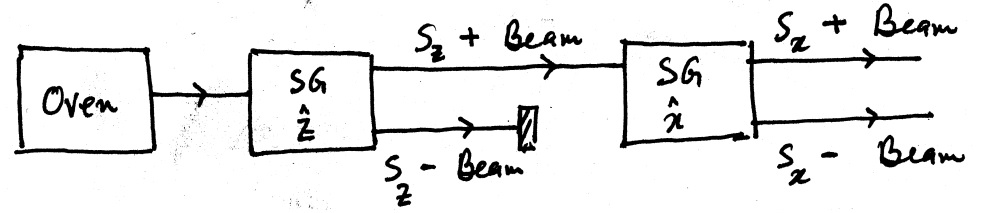
\includegraphics[scale=0.6]{sg.jpg}
	\vspace{-0.4 cm}
	\caption{Stern-Gerlach apparatus for electron spin. }
	\label{sg}
\end{figure}

Silver atoms from an oven are made to pass through a Stern-Gerlach arrangement in which the inhomogeneity in the magnetic field is 
along the $z$-axis ((SG $\hat{z}$). The beam divides into two components of equal intensity. In one of the beams all the silver atoms are in the $|S_z,\, +\rangle$ state and in the other beam all of the atoms are in the $|S_z,\,-\rangle$ state. 

\paragraph{}
Now, suppose that the $|S_z,\,-\rangle$ beam is blocked. The other beam is allowed to pass through a second Stern-Gerlach apparatus in which the inhomogeneity of the magnetic field is along the $x$-axis (SG $\hat{x}$). We find that the $|S_z,\,+\rangle$
beam which entered the SG $\hat{x}$ apparatus divides into two beams of equal intensities. This shows that if electrons are in  the state  $|S_z,\,+ \rangle$, then there is an equal probability that a
measurement of $S_x$ will give $\frac{1}{2}\hbar$ or $-\frac{1}{2}\hbar$.

\newpage

\section{Eigenvalues and Eigenvectors of $\hat{\vec{S}}. \hat{n}$ }
So far we have found the eigenvalues and the eigenvectors of the operators $\hat{S}_x$, $\hat{S}_y$ and
$\hat{S}_z$. We shall now find an expression for the eigenvectors of the operator $\hat{\vec{S}}.\hat{n}$ in the 
$|S_z,\, \pm\rangle$ basis. Here $\hat{n}$ is an arbitrary direction characterized by the polar angle $\theta$ and the azimuthal angle $\phi$ (figure below).
\begin{figure}[h]
	\centering
	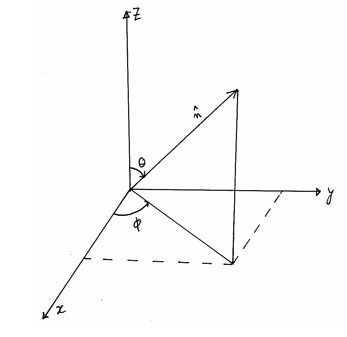
\includegraphics[scale=0.9]{direction.jpg}
	\vspace{-0.5 cm}
	\caption{A direction $\hat{n}$ in space is characterized by two angles in the spherical coordinate system, namely, the polar angle
		$\theta$ and the azimuthal angle $\phi$. }
	\label{fig:direction}
\end{figure}

The operator $\hat{\vec{S}}.\hat{n}$ represents the component of the spin angular momentum along $\hat{n}$. We can write $\hat{n}$ as
\begin{eqnarray}
\hat{n} & = & \hat{i}\,n_x + \hat{j}\, n_y + \hat{k}\, n_z \nonumber \\
& = & \hat{i}\, \sin\theta\, \cos \phi + \hat{j}\, \sin\theta\, \sin \phi + \hat{k}\, \cos\theta \, . 
\label{eq:nhat}
\end{eqnarray}

\paragraph{}
Now, the matrix representation of the operator $\hat{\vec{S}}.\hat{n}$ in the $|S_z,\,\pm\rangle$ basis is 
$\frac{1}{2} \hbar\, \vec{\sigma}.\hat{n}$. Therefore,

\be
\left( \hat{\vec{S}}.\hat{n}\right)^2 \stackrel{.}{=} \left(\frac{1}{2}\hbar\, \vec{\sigma}.\hat{n} \right)^2
= \frac{\hbar^2}{4} \left( \vec{\sigma}.\hat{n}\right)^2 = \frac{\hbar^2}{4} I\, .
\ee
Hence, the eigenvalues of $\hat{\vec{S}}.\hat{n}$ are $\pm \, \hbar/2$.

\paragraph{}
Let us now find the eigenvectors of $\hat{\vec{S}}.\hat{n}$ with eigenvalues $+\frac{1}{2}\, \hbar$. First, we write the eigenvalue equation:
\be 
\hat{\vec{S}}.\hat{n}\, |S_n,\, +\rangle = \frac{1}{2} \, \hbar \, |S_n,\, +\rangle\, . 
\label{eq:eigenvalue1}
\ee
In the $\{ |S_z,\,+\rangle,\, |S_z,\,-\rangle\}$ basis, the matrix representation of the operator $\hat{\vec{S}}.\hat{n}$ is
\begin{eqnarray}
\hat{\vec{S}}.\hat{n} &\stackrel{.}{=}& \frac{1}{2}\, \hbar\, \vec{\sigma}.\hat{n} \nonumber \\
& = & \frac{1}{2}\, \hbar\, \sigma_x \sin\theta\, \cos \phi + \frac{1}{2}\, \hbar\, \sigma_y \sin\theta\, \sin \phi
+ \frac{1}{2}\, \hbar\, \sigma_z \cos\theta \nonumber \\
& = & \frac{1}{2}\, \hbar\, \begin{pmatrix} \cos \theta & \sin\theta e^{-i\phi} \\
\sin\theta\, e^{i\phi}& -\cos\theta
\end{pmatrix}.
\end{eqnarray}		
Let the matrix representation of $|S_n,\,+\rangle$ in the same basis be
\be
|S_n,\,+\rangle \stackrel{.}{=} \begin{pmatrix}x_1\\x_2\end{pmatrix},
\ee
i.e.,
\be
\langle S_z,\,+|S_n,\,+\rangle = x_1, \quad {\rm and} \quad			
\langle S_z,\,-|S_n,\,+\rangle = x_2																	.
\ee
Therefore, the matrix representation of the eigenvalue equation (\ref{eq:eigenvalue1}) is
\[ \frac{1}{2}\, \hbar\, \begin{pmatrix} \cos \theta & \sin\theta e^{-i\phi} \\
\sin\theta\, e^{i\phi}& -\cos\theta
\end{pmatrix}\begin{pmatrix}x_1\\x_2\end{pmatrix} = 
\frac{1}{2}\,\hbar\, \begin{pmatrix}x_1\\x_2\end{pmatrix}. \]
Canceling the factor $\frac{1}{2}\, \hbar$ from both sides we get
\[ \begin{pmatrix} \cos \theta & \sin\theta e^{-i\phi} \\
\sin\theta\, e^{i\phi}& -\cos\theta
\end{pmatrix}\begin{pmatrix}x_1\\x_2\end{pmatrix} = 
\begin{pmatrix}x_1\\x_2\end{pmatrix}, \]
or,
\[ \begin{pmatrix}\cos\theta\,x_1+\sin\theta\,e^{-i\phi}\,x_2\\
\sin\theta\,e^{i\phi}\,x_1-\cos\theta\,x_2 \end{pmatrix} = 
\begin{pmatrix}x_1\\x_2 \end{pmatrix}. \]
Therefore,
\[ \cos \theta\, x_1 + \sin\theta\, e^{-i\phi}\, x_2 = x_1 \, , \]
i.e.,
\[ (1-\cos\theta)x_1=\sin\theta\, e^{-i\phi}\, x_2\, ,\]
or,
\[ 2\sin^2 \frac{\theta}{2}\, x_1 = 2\sin \frac{\theta}{2}\,\cos \frac{\theta}{2}\, e^{-i\phi}\,x_2\, .\]
From the above equation we get
\be
\frac{x_1}{x_2}= \frac{e^{-i\phi/2}\cos \theta/2}{e^{i\phi/2}\sin \theta/2}\, .
\ee
Hence, the normalized matrix representation for the state $|S_n,\,+\rangle$ is
\begin{eqnarray}
|S_n,\,+\rangle &\stackrel{.}{=}& \begin{pmatrix}e^{-i\phi/2}\cos \theta/2\\ e^{i\phi/2}\sin\theta/2\end{pmatrix} \nonumber \\
& = & e^{-i\phi/2}\, \cos \theta/2 \begin{pmatrix}1\\0\end{pmatrix} + e^{i\phi/2}\, \sin \theta/2\begin{pmatrix}0\\1\end{pmatrix}.
\end{eqnarray}
The above equation can be written in terms of the abstract vectors in the Hilbert space as
\be
\boxed{
	|S_n,\,+\rangle = e^{-i\phi/2}\, \cos \frac{\theta}{2}\, |S_z,\, +\rangle + e^{i\phi/2}\, \sin \frac{\theta}{2}\,|S_z,\,-\rangle\, .
}
\ee


\paragraph{}
Proceeding in a similar fashion, we can find the matrix representation of $|S_n,\,-\rangle$ in the
$\{ |S_z,\,+\rangle,\, |S_z,\,-\rangle\}$ basis. We get 
\be
|S_n,\,-\rangle \stackrel{.}{=} \begin{pmatrix} -e^{-i\phi/2}\sin \theta/2\\e^{i\phi/2}\cos \theta/2\end{pmatrix},
\ee
i.e.,
\be
\boxed{
	|S_n,\,-\rangle = -e^{-i\phi/2}\sin \theta/2\, |S_z,\,+\rangle   +  e^{i\phi/2}\cos \theta/2\, |S_z,\,-\rangle\, .
}
\ee




% New section
\section{Non-relativistic Description of a Spin-1/2 Particle}
\subsection{Basis Vectors}
So far we have considered quantum mechanical description of a system having spatial degrees of freedom or spin degrees
of freedom only. But a system, an electron say, can have both spatial and spin degrees of freedom. How is our fromulation
to be generalized to include both these degrees of freedom?

\paragraph{}
We note that to describe a quantum system we first need to establish a basis of states. The basis set could be written in many different ways. To set up a basis, we need a complete set of cummutating observables (CSCO) of the system and the simultaneous 
eigenstates of these observables could serve as a basis.

\paragraph{}
For a point particle with spin, the CSCO can be chosen in various ways as shown below:
\[ \{\hat{\vec{R}}, \hat{S}^2, \hat{S}_z\} \]
\[ \{\hat{\vec{P}}, \hat{S}^2, \hat{S}_z\} \]
\[ \{\hat{H}, \hat{L}^2, \hat{L}_z,\hat{S}^2, \hat{S}_z\}. \]
We shall use the first set of CSCO. Let $|\vec{r}\rangle$ and $|\epsilon\rangle$ be the eigenkets of $\hat{\vec{R}}$ and
$\{ \hat{S}^2,\, \hat{S}_z\}$, respectively, i.e.,
\begin{eqnarray}
\hat{\vec{R}}\, |\vec{r}\rangle &=& \vec{r}\, |\vec{r}\rangle \\
\hat{S}^2\, |\epsilon\rangle & =& s(s+1)\hbar^2\, |\epsilon\rangle \\
\hat{S}_z\, |\epsilon\rangle & =& \frac{1}{2}\, \hbar\,\epsilon |\epsilon\rangle \quad (\epsilon = 2 m_s).
\end{eqnarray}
For a spin-1/2 particle, $s=1/2$, therefore, there are only two possible linearly independent basis states with
$\epsilon=1$ and $\epsilon=-1$, corresponding to the $z$-component of spin being equal to $\frac{1}{2}\, \hbar$
and $-\frac{1}{2}\, \hbar$, respectively. In other words
\be
\hat{S}^2 |\pm\rangle = \frac{3}{4}\, \hbar^2\, |\pm\rangle \, , 
\ee
\be
\hat{S}_z |\pm\rangle = \pm \frac{1}{2}\, \hbar\, |\pm\rangle \, ,
\ee
where we have labelled the states as $|+\rangle \equiv |\epsilon = 1\rangle$ and $|-\rangle \equiv |\epsilon = -1\rangle$.
Now, since the space and spin degrees of freedom are independent, we have
\be
[\hat{\vec{R}},\hat{\vec{S}}]=0\, .
\ee
The simultaneous eigenkets $|\vec{r},\epsilon\rangle$ of the CSCO $\{\hat{\vec{R}}, \hat{S}^2, \hat{S}_z\}$
can then be written as a product
\be
|\vec{r}, \epsilon\rangle = |\vec{r}\,\rangle |\epsilon\rangle\, .
\label{eq:tensorproduct}
\ee
That is, the ket space formed by the eigenkets of $\{\hat{\vec{R}}, \hat{S}^2, \hat{S}_z\}$ is a tensor product of the ket space
spanned by the eigenkets $|\vec{r}\,\rangle$ of $\hat{\vec{R}}$ and the eigenkets $|\epsilon\rangle$ of
$\{\hat{S}^2, \hat{S}_z\}$. Thus
\be
H= H_{\vec{r}} \otimes H_s \, .
\ee
The orthogonality and completeness conditions of the basis kets $|\vec{r},\epsilon\rangle$ are
\be
\langle \vec{r}^{\,\,\prime}\, \epsilon^{\prime}|\vec{r}\, \epsilon \rangle = \delta(\vec{r}\, - \vec{r}^{\,\,\prime}\,)
\delta_{\epsilon\epsilon^{\prime}}
\ee
and
\be
\sum_{\epsilon}\int d^3r\, |\vec{r}\,\epsilon\rangle\langle \vec{r}\,\epsilon| = \hat{I}\, .
\label{eq:completeness}
\ee
For spin-1/2 particles, $\epsilon=\pm$, and the completeness condition, i.e., Eq. (\ref{eq:completeness}) can be written more explicitly as
\be
\int d^3r\, |\vec{r}\, +\rangle\langle \vec{r}\,+| + \int d^3r\, |\vec{r}\, -\rangle\langle \vec{r}\, -| = \hat{I}\, .
\ee


\subsection{State Vector}

Any general state $|\psi\rangle$ of the particle can be expanded as a linear combination of the basis kets
$|\vec{r}\, \epsilon\rangle$:
\begin{eqnarray}
|\psi\rangle &= & \sum_{\epsilon} \int d^3r\, |\vec{r}\, \epsilon\rangle \langle \vec{r}\, \epsilon|\psi\rangle \nonumber \\
& = & \sum_{\epsilon}\int d^3r\, |\vec{r}\, \epsilon\rangle \, \psi_{\epsilon}(\vec{r}\,)
\end{eqnarray}
where we have defined
\be
\psi_{\epsilon}(\vec{r}\,) = \langle \vec{r}\, \epsilon|\psi\rangle\, .
\ee
The numbers $\psi_{\epsilon}(\vec{r}\,)$ which depend on three continuous indices (i.e., $x$, $y$ and $z$) and on one
discrete index $\epsilon$ ( $+$ or $-$ for a spin-1/2 particle), can be considered as the `coordinates' of the state
$|\psi\rangle$ in the $|\vec{r}\, \epsilon\rangle$ basis. Thus, in order to characterize the state of a spin-1/2 particle
completely, we have to specify \underline{two} functions of the space variables $x$, $y$ and $z$:
\be
\psi_+(\vec{r}\,) \equiv \langle \vec{r},\, +|\psi\rangle, \quad {\rm and} \quad
\psi_-(\vec{r}\,) \equiv \langle \vec{r},\, -|\psi\rangle.
\ee
These two functions are often written in the form of a two-component column matrix, called a spinor, which we shall
denote as $[\psi](\vec r\,)$, i.e.,
\be 
[\psi](\vec{r}\,) = \begin{pmatrix}\psi_+(\vec{r}\,)\\\psi_-(\vec{r}\,)\end{pmatrix}.
\ee
The bra $\langle \psi|$ associated with the ket $|\psi\rangle$ is given by
\begin{eqnarray}
\langle \psi| &=& \sum_{\epsilon} \int d^3r\, \langle \psi|\vec{r}\, \epsilon\rangle \langle \vec{r}\, \epsilon| \nonumber \\
& = & \sum_{\epsilon} \int d^3r\, \psi_{\epsilon}^*(\vec{r}\,)\langle \vec{r}\,\epsilon|\, .
\end{eqnarray}
The bra $\langle \psi|$ is thus represented by two functions $\psi_+^*(\vec{r}\,)$ and $\psi_-^*(\vec{r}\,)$, written
as a row matrix which is the adjoint of $[\psi](\vec{r}\,)$. Thus
\be
\langle \psi| \stackrel{.}{=} [\psi]^{\dagger}(\vec{r}\,) = \begin{pmatrix} \psi_+^*(\vec{r}\,)&\psi_-^*(\vec{r}\,)\end{pmatrix}.
\ee
With this notation, the scalar product of two vectors $|\psi\rangle$ and $|\phi\rangle$ can be written as
\begin{eqnarray}
\langle \psi|\phi\rangle &=& \sum_{\epsilon}\int d^3r\, \langle\psi|\vec{r}\, \epsilon\rangle\langle\vec{r}\,\epsilon|\phi\rangle \nonumber \\
& = & \sum_{\epsilon}\int d^3r\,\psi_{\epsilon}^*(\vec{r}\,)\phi_{\epsilon}(\vec{r}\,) \nonumber \\
& = & \int d^3r\, \begin{pmatrix}\psi_+^*(\vec{r}\,)&\psi_-^*(\vec{r}\,)\end{pmatrix}
\begin{pmatrix}\phi_+(\vec{r}\,)\\\phi_-(\vec{r}\,)\end{pmatrix} \nonumber \\
&= & \int d^3r\, [\psi]^{\dagger}(\vec{r}\,)	[\phi](\vec{r}\,).
\end{eqnarray}			
In particular, the normalization of the state vector $|\psi\rangle$ is expressed as
\begin{eqnarray}
\langle\psi|\psi\rangle &=& \int d^3r\, [\psi]^{\dagger}(\vec{r}\,)[\psi](\vec{r}\,) \nonumber \\
& = & \int d^3r\, \left[ |\psi_+(\vec{r}\,)|^2 + |\psi_-(\vec{r}\,)|^2\right] =1.
\end{eqnarray}		

\subsubsection{Probabilistic Interpretation of the wavefunctions $\psi_{\pm}(\vec{r}\,)$}
We have have the following interpretation for the wave functions:

\begin{itemize}
	\item 
	$|\psi_+(\vec{r}\,)|^2\, d^3r $ = 
	probability that the electron is found in a small volume $d^3r$ around $\vec{r}$ with the $z$-component of the spin 
	$\frac{1}{2}\,\hbar$. A similar interpretation holds for $|\psi_-(\vec{r}\,)|^2\, d^3r$.
\end{itemize}
If we integrate $|\psi_+(\vec{r}\,)|^2\, d^3r $ over $\vec{r}$ we get
\begin{itemize}
	\item
	$\int |\psi_+(\vec{r}\,)|^2\, d^3r$  =
	probability that the $z$-component of the electron's spin is $\frac{1}{2}\, \hbar$ irrespective of its position. Similarly
	\item
	$\int |\psi_-(\vec{r}\,)|^2\, d^3r$  =
	probability that the $z$-component of the electron's spin is $-\frac{1}{2}\, \hbar$ irrespective of its position. 
\end{itemize}

As a final comment, we note that the basis vectors for a spin-1/2 particle are tensors products of a ket belonging
to $H_{\vec{r}}$ and a ket belonging to $H_s$ (Eq. \ref{eq:tensorproduct}). However, the state vector may or may not be a
tensor product of a vector in $H_{\vec{r}}$ and a vector in $H_s$. Only in the special case when the Hamiltonian is spin-independent
the state vector $|\psi\rangle$ is of this type, i.e.,
\[ |\psi\rangle = |\phi\rangle |\alpha\rangle \, , \]
where
\[ |\phi\rangle \in H_{\vec{r}}, \quad {\rm and} \quad |\alpha\rangle \in H_s\, .\]
In this case we have
\begin{eqnarray}
\psi_{\epsilon}(\vec{r}\,) &=& \langle \vec{r}\,\epsilon|\psi\rangle \nonumber \\
&=& \left(  \langle\vec{r}\,| \langle \epsilon\,|  \right) \left( |\phi\rangle |\alpha\rangle \right) \nonumber \\
&=& \langle\vec{r}\,|\phi\rangle\langle \epsilon |\alpha\rangle \nonumber \\
&=& \phi(\vec{r}\,)c_{\epsilon},
\end{eqnarray}
where
\be
c_{\epsilon}=\langle\epsilon|\alpha\rangle\ .
\ee 


\paragraph{}
For a spin-1/2 particles $\epsilon = \pm$, and in the special case of spin-independent Hamiltonian we have
\[ \psi_+(\vec{r}\,) = \phi(\vec{r}\,)c_+ \]
and
\[ \psi_-(\vec{r}\,) = \phi(\vec{r}\,)c_-\,.\]
Therefore, the spinor $[\psi](\vec{r}\,)$ is
\be
[\psi](\vec{r}\,) = \begin{pmatrix}\psi_+(\vec{r}\,)\\\psi_-(\vec{r}\,)\end{pmatrix}
= \phi(\vec{r}\,)\begin{pmatrix}c_+\\c_-\end{pmatrix}.
\ee
The square of the norm of $|\psi\rangle$ is then given by
\be
\langle\psi|\psi\rangle= \langle\phi|\phi\rangle \langle \chi|\chi\rangle = (|c_+|^2+|c_-|^2)\int d^3r\, |\phi(\vec{r}\,)|^2\, .
\ee

\section{Electron in an External Magnetic Field. Pauli Equation}
Suppose that an electron is placed in an external time-independent magnetic field $\vec{B}$. The magnetic moment operator of the
electron is 
\be
\hat{\vec{\mu}} =  = \hat{\vec{\mu}}_{{\rm orbit}} + \hat{\vec{\mu}}_{{\rm spin}}\, ,
\ee
where
\be
\hat{\vec{\mu}}_{{\rm orbit}} = \frac{q_e}{2m_e} \hat{\vec{L}} 
\ee
and
\be
\hat{\vec{\mu}}_{{\rm spin}} =g_s \frac{q_e}{2m_e} \hat{\vec{S}}\, .
\ee
Here $q_e$ is the charge of the electron, i.e., $q_e=-e$ with $e=1.6 \times 10^{-19}$ C, and $g_s$ is the spin
gyromagnetic ratio. From Dirac theory we have $g_s=2$ for electrons. The total magnetic moment of the electron is then
\be
\hat{\vec{\mu}} = \frac{q_e}{2m_e} (\hat{\vec{L}} + 2 \hat{\vec{S}} )\, .
\ee 
In the spin space of the electron, we can express $\hat{\vec{\mu}}$ as a $2\times 2$ matrix:
\be
\hat{\vec{\mu}} = \frac{q_e}{2m_e} (\hat{\vec{L}}\; \hat{1}_{2\times 2} + \hbar \vec{\sigma} )
\ee
where we have used the matrix representation of the spin operator of a spin-1/2 particle, i.e.,
\be
\hat{\vec{S}} \stackrel {.}{=} \frac{1}{2}\,\hbar\, \vec{\sigma}\, ,
\ee
and $\hat{1}_{2\times 2}$ is a unit $2\times 2$ matrix.

\paragraph{}
Now, the interaction energy of the electron with the external magnetic field is
\begin{eqnarray}
V &=& -\hat{\vec{\mu}}.\vec{B} \nonumber \\
& = & \mu_{B}\left( \frac{\hat{\vec{L}}}{\hbar}\, \hat{1}_{2\times 2} + \vec{\sigma} \right).\vec{B} \, ,
\end{eqnarray}
where
\be
\mu_B = \frac{|q_e|\hbar}{2m_e} = \frac{e\hbar}{2m_e}\, 
\ee
is the Bohr magneton. Here $e$ is the magnitude of charge of the electron, hence $e$ is a positive number,
$e=1.6\times 10^{-19}$ C. The Hamiltonian operator of the electron is then
\be
\hat{H} = \left( \frac{\hat{\vec{p}}^{\,2}}{2m_e} + V(\hat{\vec{r}}\,) \right ) I_{2\times 2} + \mu_{B}\left( \frac{\hat{\vec{L}}}{\hbar}\, \hat{1}_{2\times 2} + \vec{\sigma} \right).\vec{B}\, ,
\ee
where $V(\hat{\vec{r}}\,)$ is the potential energy of the electron's interaction with other fields, for example, the Coulomb field of the nucleus if the electron is bound in an atomic orbit. The Schr\"{o}dinger equation for the electron is then
\be
i\hbar \frac{\partial}{\partial t}\, |\psi\rangle = \hat{H} |\psi\rangle\,,
\ee
or, in terms of the components of $|\psi\rangle$
\begin{multline}
i \hbar\, \frac{\partial}{\partial t}\, \begin{pmatrix}\psi_+(\vec{r}\, , t)\\ \psi_+(\vec{r}\, , t) \end{pmatrix}
= \\ \left[ \left( \frac{-\hbar^2}{2m_e}\, \nabla^2 + V(\vec{r}\,) + \frac{\mu_B}{\hbar}\, \hat{\vec{L}}.\vec{B}\right)
\hat{1}_{2\times 2} + \mu_B \vec{\sigma}.\vec{B}\right]
\begin{pmatrix}\psi_+(\vec{r}\, , t)\\ \psi_+(\vec{r}\, , t) \end{pmatrix}.
\end{multline}
This non-relativistic equation for a spin-1/2 particle is known as Pauli equation.

\vspace{1 cm}
\large{ \begin{center}END\end{center}}




%% writing by shahnoor

\chapter{sheet-18 : Rotations and Angular Momentum}

\ifpdf
\graphicspath{{Chapter18/figs/}}
\else
\graphicspath{{Chapter18/figs/}}
\fi

reference : Sakurai, Cohen-Tanondgi\\

A rotation of a physical system is specified by the angle of rotation and the axis of rotation. The rotation can be either positive or negative. If a right-handed screw turned in the direction of rotation proceeds along the positive direction of the axis, the rotation is said to be positive. Thus, for examp, $\phi\hat{z}$ denotes a positive rotation by an angle $\phi$ about the z-axis Fig. (\ref{chapter18.fig1})

\begin{figure}
	%%%%%%% TODO
	\centering
	
\includegraphics[width=0.5\linewidth]{Pictures/not-found.jpg}
	\caption{A positive rotation of the physical system by an angle $\phi$ about the $z$-axis.}
	\label{chapter18.fig1}
\end{figure}
In our subsequent discussions we will consider active rotation\index{active and passive rotation}, i.e., rotation of the physical system rather than the rotation of the coordinates.\\

Now, finite rotations about different axes do not commute, i.e., the change in the coordinate of a point in the physical system depends on the order the rotations are performed. To work out quantitatively the extent in which rotations about different axes fail to commute, we have to construct the matrices corresponding to rotations in the three-dimensional real space $(x,y,z)$.\\

In each rotation a vector $\vec{r}$ with coordinates $(x, y, z)$ changes to a new vector $\vec{r^\prime}$ with coordinate $(x^\prime,y^\prime,z^\prime)$. The matrix connecting $(x^\prime,y^\prime,z^\prime)$ with $(x,y,z)$ is the matrix corresponding to the rotation.

%% page 3
Thus
\begin{equation}
\label{chapter18.eqn1}
\mqty[x^\prime\\ y^\prime \\ z^\prime] = \mqty[R]  \mqty[x\\ y \\ z]
\end{equation}
Where $R$ is the $3\times3$ square matrix corresponding to the rotation. In a rotation, the length of the vector $\vec{r}$ remains unchanged, i.e.,
\begin{equation}
\norm{\vec{r^\prime}} = \sqrt{{x^{\prime}}^2 + {y^{\prime}}^2 + {z^{\prime}}^2} = \sqrt{x^2 + y^2 + z^2} =\norm{\vec{r}}
\end{equation}
Therefore, the matrix $R$ must be orthogonal, i.e.,
\begin{equation}
R^T R = R R^T = \mathcal{1}
\end{equation}
Next, we will construct explicitly the rotation matrices $R$ in the three-dimensional space corresponding to positive rotations about the $x$-axis, $y$-axis and $z$-axis.

First, consider a finite rotation by an angle $\phi$ in a positive sense about the $z$-axis (Fig. \ref{chapter18.fig2})
\begin{figure}
	%%%%%%% TODO
	\centering
	
\includegraphics[width=0.5\linewidth]{Pictures/not-found.jpg}
	\caption{A positive rotation by an angle $\phi$ about the $z$-axis.}
	\label{chapter18.fig2}
\end{figure}
We have
\begin{align*}
x^\prime = \cos\phi x - \sin\phi y \\
y^\prime = \sin\phi x + \cos\phi y
z^\prime = z
\end{align*}
In matrix form
\begin{equation*}
	\mqty[x^\prime\\ y^\prime \\ z^\prime] = \mqty[\cos\phi & - \sin\phi& 0 \\
		\sin\phi & \cos\phi & 0 \\
		0& 0& 1]  
	\mqty[x\\ y \\ z]
\end{equation*}
Thus, the rotation matrix corresponding to a positive rotation by an angle $\phi$ about the $z$-axis is 
\begin{equation}
\label{chapter18.eqn4}
R_z\qty(\phi) = \mqty[\cos\phi & - \sin\phi& 0 \\
\sin\phi & \cos\phi& 0 \\
0& 0& 1]
\end{equation}
Next, consider a rotation about the $x$-axis. The corresponding matrix is
\begin{equation}
\label{chapter18.eqn5}
R_x\qty(\phi) = \mqty[1& 0& 0 \\
0& \cos\phi & - \sin\phi\\
0& \sin\phi & \cos\phi]
\end{equation}

Similarly
\begin{equation}
\label{chapter18.eqn6}
R_y\qty(\phi) = \mqty[\cos\phi& 0& \sin\phi \\
0& 1& 0 \\
-\sin\phi& 0 &\cos\phi]
\end{equation}

%% page 6
For infinitesimal rotation, i.e., $\phi=\epsilon$, the rotation matrices, up to second order in $\epsilon$ are
\begin{align}
\label{chapter18.eqn7}
\begin{split}
R_x\qty(\epsilon) = \mqty[1 & 0 & 0 \\ 0 & 1-\frac{\epsilon^2}{2} &- \epsilon \\ 0 & \epsilon & 1 - \frac{\epsilon^2}{2}] \\
R_y\qty(\epsilon) = \mqty[1 - \frac{\epsilon^2}{2} & 0 & \epsilon \\ 0 & 1 & 0 \\ -\epsilon & 0 & 1 - \frac{\epsilon^2}{2}] \\
R_z\qty(\epsilon) = \mqty[1 - \frac{\epsilon^2}{2} & -\epsilon & 0 \\ \epsilon & 1 - \frac{\epsilon^2}{2} & 0 \\ 0 & 0 & 1]
\end{split}
\end{align}
Now the multiplication leads to (up to $\order{\epsilon^2}$)
\begin{equation}
\label{chapter18.eqn8a}
R_x\qty(\epsilon) R_y\qty(\epsilon) = \mqty[1-\frac{\epsilon^2}{2} & 0 & \epsilon\\ \epsilon^2 & 1- \frac{\epsilon^2}{2} & -\epsilon\\ -\epsilon & \epsilon & 1-\epsilon^2] + \order{\epsilon^3}
\end{equation}
and
\begin{equation}
\label{chapter18.eqn8b}
R_y\qty(\epsilon) R_x\qty(\epsilon) = \mqty[1-\frac{\epsilon^2}{2} & \epsilon^2 & \epsilon\\ 0 & 1- \frac{\epsilon^2}{2} & -\epsilon\\ -\epsilon & \epsilon & 1-\epsilon^2] + \order{\epsilon^3}
\end{equation}
From (\ref{chapter18.eqn8a}) and (\ref{chapter18.eqn8b}) we have
\begin{equation}
\label{chapter18.eqn9}
R_x(\epsilon) R_y(\epsilon) - R_y(\epsilon)  R_x(\epsilon) = \mqty[0 & -\epsilon^2 & 0 \\ \epsilon^2 & 0 & 0 \\ 0 & 0 & 0] = R_z(\epsilon^2) - 1
\end{equation}
In these calculations all terms higher than $\epsilon^2$ have been ignored. Eq. (\ref{chapter18.eqn9}) leads to the import result that infinitesimal rotations about different axes do commute up to first order. Now, we have
\begin{equation}
\label{chapter18.eqn10}
1 = R_{any}(0)
\end{equation}
where $any$ stands for any rotation axis. Thus Eq. (\ref{chapter18.eqn9}) can be written as
\begin{equation}
\label{chapter18.eqn11}
\comm{R_x(\epsilon)}{R_y(\epsilon)} = R_z(\epsilon^2) - R_{any}(0)
\end{equation}

\begin{align}
\label{chapter18.eqn12}
\comm{R_y(\epsilon)}{R_z(\epsilon)} = R_x(\epsilon^2) - R_{any}(0)\\
\label{chapter18.eqn13}
\comm{R_z(\epsilon)}{R_x(\epsilon)} = R_y(\epsilon^2) - R_{any}(0)
\end{align}

Eqs. (\ref{chapter18.eqn11}) to (\ref{chapter18.eqn13}) are examples of the commutation relations between rotational matrices in three dimensional real space. These commutation relations will be used later to derived the angular momentum commutation relations.



\section{Rotations in Hilbert Space}
%% page 9

Consider a physical system with state vector $\ket{\psi}$ in Hilbert space.
\begin{figure}
	%%%%%%% TODO
	\centering
	
\includegraphics[width=0.5\linewidth]{Pictures/not-found.jpg}
	\caption{rotation in Hilbert space}
	\label{chapter18.fig3}
\end{figure}
If the system is now rotated by a certain angle about a certain axis, the state vector changes to $\ket{\psi}_R$. Thus there exists an operator $U(R)$ in Hilbert space which carries the state $\ket{\psi}$ to $\ket{\psi}_R$, i.e.,
\begin{equation}
\label{chapter18.eqn14}
\ket{\psi}_R = U(R) \ket{\psi}
\end{equation}
The operator $U(R)$ is unitary so that normalization of the states remain unaltered.


What we have done is to established a correspondence between a rotation in real three-dimensional space and a unitary operator $U(R)$ in the Hilbert space,
\begin{align*}
R &\longleftrightarrow U(R) \\
\qq{Rotation in 3-space}& \longleftrightarrow \qq{Transformation in Hilbert space}
\end{align*}
Note that $R$ is a $3\times 3$ orthogonal matrix acting on the components of a classical vector in $3$-space while $U(R)$ is a unitary operator acting on the \textit{vectors} of a Hilbert space (ket space). We could also find a matrix representation of the operator $U(R)$ in the Hilbert space by choosing an appropriate set of basis kets. If the number of kets in the basis set is $N$, then the matrix representation of $U(R)$ would be $N\times N$ dimensional.

%% page 11
For example, if we consider a spin-$1/2$ particle with no other degrees of freedom, then $N=2$ and $U(R)$ would be a $2\times 2$ unitary matrix, for a spin-$3/2$ particle with no other degrees of freedom, $N=4$, and $U(R)$ would be a $4\times 4$ unitary matrix.\\


Now, we will construct the unitary operator $U(R)$. To do so, it is advantageous to consider infinitesimal rotations of the physical system. To be specific, suppose the physical system is rotated by an infinitesimal angle $\dd{\phi}$ about the $z$-axis. Therefore
\begin{equation}
R = \hat{z} \dd{\phi}
\end{equation}
We can write $U(R)$ as
\begin{equation}
\label{chapter18.eqn15}
U(\dd{\phi} \hat{z}) = 1 - \frac{J_z}{\hbar} \dd{\phi}
\end{equation}
where $J_z$ is a hermitian operator with dimensions of action (i.e., dimensions of $\hbar$ : $\qq{Energy}\times \qq{Time}$ or $\qq{Position}\times \qq{Momentum}$). At this state $J_z$ is \textbf{not} yet identified with the $z$-component of the total angular momentum operator. This identification will be made later after we derive the commutations of $J_z$ with other generators.\\

In Eq. (\ref{chapter18.eqn15}), $J_z$ is the generator of the unitary operator $U(\dd{\phi} \hat{z})$. The operator $U(\phi \hat{z})$ corresponding to a finite positive rotation $\phi$ about the $z$-axis can be obtained by successively compounding infinitesimal rotations about the same axis. Thus
\begin{align}
U_z(\phi) 
&= \lim\limits_{N \rightarrow \infty} \qty[1 - \frac{\iu J_z}{\hbar} \frac{\phi}{N}]^N \nonumber\\
\label{chapter18.eqn16a}
&= e^{-\iu J_z \phi/\hbar} \\
\label{chapter18.eqn16b}
&= 1 - \frac{\iu J_z \phi}{\hbar} - \frac{J_z^2 \phi^2}{2 \hbar^2}
\end{align}
Similarly we can write
\begin{align}
\label{chapter18.eqn17}
U_x(\phi) &= e^{-\iu J_x \phi/\hbar} \\
\label{chapter18.eqn18}
U_y(\phi) &= e^{-\iu J_y \phi/\hbar}
\end{align}
In general, for a positive rotation by an angle $\phi$ about an axis $\hat{n}$, we have
\begin{align}
\label{chapter18.eqn19}
U_{\hat{n}}(\phi) &= e^{-\iu \vec{J}\cdot\hat{n} \phi/\hbar}
\end{align}
From Eqs. (\ref{chapter18.eqn16a}), (\ref{chapter18.eqn17}) and (\ref{chapter18.eqn18}) we note that the hermitian operators $J_x,\ J_y$ and $J_z$ are the generators of the unitary transformation operaors in the Hilbert space if the system is rotated about the $x$, $y$ and $z$-axis, respectively. We will now show that the three generators $J_x,\ J_y$ and $J_z$ obey the commutation relations of angular momentum operators.



\section{Commutation relations of $J_x,J_y,J_z$}
%% page 14

To obtain the commutation relations between $J_x,\ J_y$ and $J_z$, we need the concept of a group (see Appendix (\ref{appendix4.group})). Now, the rotations form a group. The group multiplication is the application of two rotations successively. To see that the set of all rotations of a physical system form a group, we note that two successive rotations is equivalent to one single rotation. The inverse of a rotation $\phi \hat{n}$ is $-\phi\hat{n}$. The unit element is no rotation at all.\\


To every rotation of the physical system there corresponds a $3\times 3$ orthogonal matrix $R$ acting on the coordinates of a classical vectors, and a unitary operator $U(R)$ acting on the state kets in the Hilbert space. We say that the $3\times 3$ orthogonal matrices $R$ is a representation of the rotation group in the ordinary $3$-space. The set of unitary operator $U(R)$ is also a representation of the rotation group but in the Hilbert space of state vectors. Thus we may postulate $U(R)$ has the same group properties as $R$
\begin{table}
	\begin{tabular}{c|c|c}
		identity & $1\cdot R = R\cdot 1 = R$ & $\mathbb{1} U(R) = U(R) \mathbb{1} = U(R)$ \\ \hline
		closure & $R_1 R_2 = R_3$ & $U(R_1) U(R_2) = U(R_3)$ \\ \hline
		inverse & $R \cdot R^{-1} = 1 = R^{-1}\cdot R$ & 
			\begin{minipage}{5cm}
				\begin{align*}
				U(R) U(R^{-1}) = \mathbb{1} =  U(R^{-1})  U(R)\\
				\therefore  U(R^{-1}) =  U^{-1}(R) 
				\end{align*}
			\end{minipage}\\ \hline
		associativity & 
		\begin{minipage}{5cm}
			\begin{align*}
			R_1 \cdot (R_2 \cdot R_3) \\
			= (R_1 \cdot R_2) \cdot R_3 \\
			= R_1 \cdot R_2 \cdot R_3
			\end{align*}
		\end{minipage}
			 & 
		\begin{minipage}{5cm}
			\begin{align*}
			U(R_1)\qty(U(R_2) U(R_3)) \\
			= \qty(U(R_1)U(R_2)) U(R_3)\\
			= U(R_1)U(R_2) U(R_3)
			\end{align*}
		\end{minipage}
	\end{tabular}
\end{table}

Therefore, to any equation involving the unitary operator $U(R)$. The analogue of Eq. (\ref{chapter18.eqn9}) in Hilbert space is
\begin{equation}
\label{chapter18.eqn20}
U_x(\epsilon) U_y(\epsilon) - U_y(\epsilon) U_x(\epsilon) = U_z(\epsilon^2) - 1
\end{equation}

Eqs. (\ref{chapter18.eqn9}) and (\ref{chapter18.eqn20}) are valid up to second order in $\epsilon$. We therefore expand Eq. (\ref{chapter18.eqn20}) up to second order obtaining
\begin{equation}
\label{chapter18.eqn21}
\begin{split}
\qty(1 - \frac{\iu J_x \epsilon}{\hbar} - \frac{J_x^2 \epsilon^2}{2 \hbar^2}) 
\qty(1 - \frac{\iu J_y \epsilon}{\hbar} - \frac{J_y^2 \epsilon^2}{2 \hbar^2})
-
\qty(1 - \frac{\iu J_y \epsilon}{\hbar} - \frac{J_y^2 \epsilon^2}{2 \hbar^2})
\qty(1 - \frac{\iu J_x \epsilon}{\hbar} - \frac{J_x^2 \epsilon^2}{2 \hbar^2})\\
= \qty(1 - \frac{\iu J_z \epsilon^2}{\hbar}) - 1
\end{split}
\end{equation}
Terms of the order $\epsilon$ automatically drop out. Equating terms of order  $\epsilon^2$ on both sides of Eq. (\ref{chapter18.eqn21}) we obtain

\begin{equation}
\label{chapter18.eqn22}
\comm{J_x}{J_y} = \iu \hbar J_z
\end{equation}

Repeating this kind of arguments with rotations about other axes, we obtain
\begin{align}
\label{chapter18.eqn23}
\comm{J_y}{J_z} = \iu \hbar J_x \\
\label{chapter18.eqn24}
\comm{J_z}{J_x} = \iu \hbar J_y
\end{align}
Equations (\ref{chapter18.eqn22}) to (\ref{chapter18.eqn24}) are the fundamental commutation relation of angular momentum operators.
We can combine Eqs. (\ref{chapter18.eqn22}) to (\ref{chapter18.eqn24}) as
\begin{equation}
	\comm{J_i}{J_j} = \iu \hbar \varepsilon_{i j k} J_k
\end{equation}
Where $\varepsilon_{i j k}$ is the levi-civita symbol.


 We thus conclude that the generators of the unitary transformations of state vectors in Hilbert space corresponding to rotations of the physical system are nothing but the angular momentum operators.




\section{Rotation operator applied to a spinless particle}
%%% page 21
Suppose that a system is rotated by an angle $\phi$ about an axis $\hat{n}$ in the positive sense. The state of the system changes from $\ket{\psi}$ to $\ket{\psi^\prime}$ according to 
\begin{equation}
\label{chapter18.eqn1-spinless}
\ket{\psi^\prime} = U_{\hat{n}}\qty(\phi) \ket{\psi}
\end{equation}
where
\begin{equation}
\label{chapter18.eqn2-spinless}
	 U_{\hat{n}}\qty(\phi) = e^{-i \vec{J}\cdot\hat{n} \phi/\hbar}
\end{equation}
Now, if the system is a spinless particle $(\vec{S}=0)$ then $\vec{J} = \vec{L}$ and the corresponding rotation operator is
\begin{equation}
\label{chapter18.eqn3-spinless}
U_{\hat{n}}\qty(\phi) = e^{-i \vec{L}\cdot\hat{n} \phi/\hbar}
\end{equation}
For simplicity, we will consider rotation about the $z$-axis and see how the wavefunction changes under such a rotation.
\begin{figure}
	%%%%%%% TODO
	\centering
	
\includegraphics[width=0.5\linewidth]{Pictures/not-found.jpg}
	\caption{rotation in Hilbert space}
	\label{chapter18.fig4}
\end{figure}
In this case we have
\begin{align}
\ket{\psi^\prime} 
&= U_{z}\qty(\phi) \ket{\psi} \nonumber\\
\label{chapter18.eqn4-spinless}
&= e^{-i L_z \phi/\hbar} \ket{\psi}
\end{align}
In coordinate representation Eq. (\ref{chapter18.eqn4-spinless}) is
\begin{equation}
\label{chapter18.eqn5-spinless}
\braket{\vec{r}}{\psi^\prime} = \mel{\vec{r}}{e^{-i L_z \phi/\hbar}}{\psi}
\end{equation}
%% page 23
Now
\begin{equation*}
\bra{\vec{r}} \hat{L}_z = \bra{\vec{r}} \qty(\hat{\vec{r}} \times \hat{\vec{p}})_z = \qty(\hat{\vec{r}} \times \frac{\hbar}{\iu} \vec{\nabla})_z \bra{\vec{r}}
\end{equation*}
Therefore, Eq. (\ref{chapter18.eqn5-spinless}) can be written as
\begin{equation}
\braket{\vec{r}}{\psi^\prime} = e^{-\frac{\iu}{\hbar} \phi \qty(\vec{r} \times \frac{\hbar}{\iu} \vec{\nabla})_z} \braket{\vec{r}}{\psi}
\end{equation}
For infinitesimal rotations $\dd{\phi}$ we have
\begin{align*}
\psi^\prime\qty(\vec{r}) 
&= \qty[1 - \frac{\iu}{\hbar} \dd{\phi} \qty(\vec{r} \times \frac{\hbar}{\iu} \vec{\nabla})_z] \psi\qty(\vec{r}) \\
&= \qty[1 - \dd{\phi} \qty(x \pdv{}{y} - y \pdv{}{x})] \psi\qty(\vec{r}) \\
&= \psi\qty(\vec{r}) - \dd{\phi} x \pdv{\psi(x,y,z)}{y} + \dd{\phi} y \pdv{\psi(x,y,z)}{x} \\
&= \psi\qty(x + y\dd{\phi}, y - x \dd{\phi}, z)
\end{align*}

Now
\begin{align}
\label{chapter18.eqn1.infinitesimal-3d}
R_z(\dd{\phi}) &= \mqty[1 & -\dd{\phi} & 0 \\ \dd{\phi} & 1 & 0 \\ 0 & 0 & 1] \\
\label{chapter18.eqn2.infinitesimal-3d}
\therefore R^{-1}_z(\dd{\phi}) &= \mqty[1 & \dd{\phi} & 0 \\ -\dd{\phi} & 1 & 0 \\ 0 & 0 & 1] \\
\end{align}
Therefore
\begin{equation*}
R^{-1}_z(\dd{\phi}) \vec{r} = \mqty[1 & \dd{\phi} & 0 \\ -\dd{\phi} & 1 & 0 \\ 0 & 0 & 1]  \mqty[x\\y\\z] = \mqty[x+y\dd{\phi} \\ y - x\dd{\phi} \\ z]
\end{equation*}
Hence
\begin{equation}
\label{chapter18.eqn6-spinless}
\psi^\prime(\vec{r}) = \psi(R^{-1} \vec{r})
\end{equation}
Since $\vec{r}$ is arbitrary in Eq. (\ref{chapter18.eqn6-spinless}), we can rewrite (\ref{chapter18.eqn6-spinless}) in the form
\begin{equation}
\label{chapter18.eqn7-spinless}
\psi^\prime(R \vec{r}) = \psi(\vec{r})
\end{equation}
Eq. (\ref{chapter18.eqn7-spinless}) is intuitively obvious. If the system is rotated, the old wave function at any point $\vec{r}$ must be equal to the new wave function at the rotated point $R\vec{r}$.

We have derived the transformation equation of the wavefunction (Eq. (\ref{chapter18.eqn6-spinless}) or (\ref{chapter18.eqn7-spinless})) of a spinless particle using the expression rotation operator given in Eq. (\ref{chapter18.eqn3-spinless}). We could \textit{work backwards}, i.e., starting from the obvious transformation of the wavefunction under rotation, i.e., Eq. (\ref{chapter18.eqn6-spinless}) or (\ref{chapter18.eqn7-spinless}),  we could work out the expression for the rotation operator in the Hilbert space of spinless particles.


Thus, if the system is rotated by an angle $\phi$ about the $z$-axis, the wave function changes from $\phi(\vec{r})$ to $\psi^\prime(\vec{r})$ in such a manner that
\begin{equation}
\label{chapter18.eqn8-spinless}
	\psi^\prime(\vec{r}) = \psi\qty(R^{-1}_z(\phi) \vec{r})
\end{equation}
We cast Eq. (\ref{chapter18.eqn8-spinless}) in the form
\begin{equation}
\label{chapter18.eqn9-spinless}
	\psi^\prime(\vec{r}) = U_z(\phi) \psi(\vec{r})
\end{equation}
where $U_z(\phi)$ is the rotation operator in the Hilbert space. To express Eq. (\ref{chapter18.eqn8-spinless}) in the form Eq. (\ref{chapter18.eqn9-spinless}), it is convenient to consider infinitesimal rotations in Eq. (\ref{chapter18.eqn2.infinitesimal-3d}) and Eq. (\ref{chapter18.eqn8-spinless}) is

\begin{align*}
\psi^\prime(\vec{r}) 
&= \psi(x + y\dd{\phi}, y - x\dd{\phi}, z) \\
&= \psi\qty(\vec{r}) - \dd{\phi} x \pdv{\psi(x,y,z)}{y} + \dd{\phi} y \pdv{\psi(x,y,z)}{x} \\
&= \qty[1 - \dd{\phi} \qty(x \pdv{}{y} - y \pdv{}{x})] \psi\qty(\vec{r}) \\
&= \qty[1 - \frac{\iu}{\hbar} \dd{\phi} \qty(\vec{r} \times \frac{\hbar}{\iu} \vec{\nabla})_z] \psi\qty(\vec{r}) \\
&= \qty[1 - \frac{\iu}{\hbar} \dd{\phi} \qty(\vec{r} \times \vec{p})_z] \psi(x,y,z) \\
&= \qty[1 - \frac{\iu}{\hbar} \dd{\phi} \hat{L}_z] \psi(x,y,z)
\end{align*}
For a finite rotation we have
\begin{equation}
\label{chapter18.eqn11-spinless}
\psi^\prime(\vec{r}) = e^{-\frac{\iu}{\hbar} \phi \hat{L}_z}  \psi(\vec{r})
\end{equation}
Hence, the rotation operator in Hilbert space  of a spin particle is given by Eq. (\ref{chapter18.eqn3-spinless}).



\section{Rotation operator in spin space}
\label{chapter28.sect.rotation-in-spin-space}
%% page 27
Consider a particle with only spin degrees of freedom, i.e., the particle's spatial degrees of freedom are suppressed. In this case $\vec{L} = 0$, and, therefore, $\vec{J}=\vec{S}$ where $\vec{S}$ is the spin angular momentum operator of the particle. The rotation operator in the spin Hilbert space is then 
\begin{equation}
\label{chapter18.eqn13-spin}
U^{(s)}_{\hat{n}}\qty(\phi) = e^{- \frac{\iu}{\hbar} \vec{S}\cdot\hat{n} \phi}
\end{equation}

Consider now a rotation by a finite angle $\phi$ about the $z$-axis. If the ket of a spin-$1/2$ particle before rotation in $\ket{\alpha}$, the ket after rotation in given by
\begin{equation}
\label{chapter18.eqn14-spin}
\ket{\alpha}_R = U^{(s)}_{z}\qty(\phi) \ket{\alpha} = e^{- \frac{\iu}{\hbar} S_z \phi} \ket{\alpha}
\end{equation}

To show that the operator (\ref{chapter18.eqn13-spin}) really rotates the physical system, let us look at its effects on $\expval{S_x}$. Under the rotation about the $z$-axis, this expectation value changes to
\begin{equation}
\expval{S_x} \rightarrow \expval{S_x}^\prime = \tensor[_R]{\mel{\alpha}{S_x}{\alpha}}{_R} = \mel{\alpha}{U^{\dagger}_z(\phi) S_x U_z(\phi)}{\alpha}
\end{equation}
We must therefore compute $U^{\dagger}_z(\phi) S_x U_z(\phi)$. Using the identity
\begin{equation}
e^{A} B e^{-A} = B + \comm{A}{B} + \frac{1}{2 !} \comm{A}{\comm{A}{B}} + \ldots
\end{equation}

we have
\begin{align*}
U^{\dagger}_z(\phi) S_x U_z(\phi) 
&= e^{ \frac{\iu}{\hbar} S_z \phi} S_x e^{- \frac{\iu}{\hbar} S_z \phi} \\
&= S_x + \qty(\frac{\iu \phi}{\hbar}) \comm{S_z}{S_x} + \frac{1}{2 !} \qty(\frac{\iu \phi}{\hbar})^2 \comm{S_z}{\comm{S_z}{S_x}} + \frac{1 }{3 !} \qty(\frac{\iu \phi}{\hbar})^3 \comm{S_z}{\comm{S_z}{\comm{S_z}{S_x}}}  + \ldots \\
&= S_x + \qty(\frac{\iu \phi}{\hbar}) \iu \hbar S_y + \frac{1}{2 !} \qty(\frac{\iu \phi}{\hbar})^2 \hbar^2 S_x + \frac{1}{3 !} \qty(\frac{\iu \phi}{\hbar})^3 \iu \hbar^3 S_y + \ldots \\
&= S_x \qty(1 - \frac{\phi^2}{2 !} + \ldots)  - S_y \qty(\phi - \frac{\phi^3}{3 !} + \ldots) \\
&= S_x \cos\phi - S_y \sin\phi
\end{align*}

Thus
\begin{equation}
\expval{S_x}^\prime = \expval{S_x} \cos\phi - \expval{S_y}\sin\phi
\end{equation}
Similarly
\begin{align}
\label{chapter18.eqn15-spin}
\expval{S_y}^\prime = \expval{S_x} \sin\phi + \expval{S_y}\cos\phi \\
\expval{S_z}^\prime = \expval{S_z}
\end{align}
This shows that the \textit{rotation} operator (\ref{chapter18.eqn13-spin}) when applied to the state ket does rotate the expectation value of $\vec{S}$ around the $z$-axis by an angular $\phi$. In other words, the expectation values of the spin operator behaves as though it ware a classical vector!

Up to now we have dealt with the expectation values of the spin operator in the rotated and unrotated spin states. Now let us look at the effect of the rotation $U_z(\phi)$ on a general spin state $\ket{\alpha}$. For a spin $1/2$ particle we write
\begin{equation}
\label{chapter18.eqn16-spin}
\ket{\alpha} = \ket{+} \braket{+}{\alpha} + \ket{-} \braket{-}{\alpha}
\end{equation}
where $\ket{\pm}$ are the eigenstates of $S_z$ with eigenvalues $\pm \frac{1}{2} \hbar$. Now
\begin{equation}
e^{-\iu S_z \phi/\hbar} \ket{\alpha} = e^{-\iu \phi/2} \ket{+} \braket{+}{\alpha} + e^{\iu \phi/2} \ket{-} \braket{-}{\alpha}
\end{equation}
The appearance of the half angle $\phi/2$ here has an extremely interesting consequence. Let us consider a rotation by an angle $2\pi$. We then have
\begin{equation}
\label{chapter18.eqn17-spin}
\ket{\phi} \substack{\rightarrow \\ R_z(2 \pi)} \ket{\alpha}_R = - \ket{\alpha}
\end{equation}
So that the ket for the $360^\circ$ rotated state differs from the original ket by a minus sign. We would require a $720^\circ$ or $\phi=4 \pi$ rotation to get back to the same state with plus sign. Notice that this minus sign disappears from the expectation of $\vec{S}$ because $\vec{S}$ is sandwiched between $\bra{\alpha}$ and $\ket{\alpha}$, both of which change sign. (Will this minus sign be observable ? see Sakurai)



\subsection{Matrix Representation}
%% page 32
The rotation operator in spin space is given by Eq. (\ref{chapter18.eqn13-spin}). For a spin-$1/2$ particle we can use the eigenkets $\ket{\pm}$ of $S_z$ as basis. Then $\vec{S}$ and $U^{(s)}_{\hat{n}}\qty(\phi)$ are expressed as $2\times 2$ matrices. We then have
\begin{equation}
\vec{S} \doteq \frac{1}{2} \hbar \vec{\sigma}
\end{equation}
Therefore
\begin{equation}
e^{-\frac{\iu}{\hbar} \vec{S}\cdot \hat{n} \phi} \doteq e^{-\iu \frac{\vec{\sigma}\cdot \hat{n}}{2} \phi}
\end{equation}

The $2\times 2$ matrices $\exp(-\iu \frac{\vec{\sigma}\cdot \hat{n}}{2} \phi)$ act on the two component spinor $\chi$ where
\begin{equation}
\chi = \mqty[\braket{+}{\alpha} \\ \braket{-}{\alpha}]
\end{equation}

Now
\begin{align*}
U_n^{(s)}\qty(\phi) 
&\doteq e^{-\iu \frac{\phi}{2} \vec{\sigma}\cdot\hat{n}} \\
&= 1 + \qty(-\frac{\iu\phi}{2}) \vec{\sigma}\cdot\hat{n} 
+ \frac{1}{2 !} \qty(-\frac{\iu\phi}{2})^2 \qty(\vec{\sigma}\cdot\hat{n})^2 + \ldots 
+ \frac{1}{m !} \qty(-\frac{\iu\phi}{2})^m \qty(\vec{\sigma}\cdot\hat{n})^m + \ldots
\end{align*}
Applying the identity
\begin{equation}
\qty(\vec{\sigma}\cdot\hat{n})^2 = \hat{n}\cdot\hat{n} 1_{2\times 2} + \iu \vec{\sigma} \cdot \qty(\hat{n} \times \hat{n}) = 1_{2\times 2}
\end{equation}
Which leads to
\begin{equation}
\qty(\vec{\sigma}\cdot\hat{n})^m = 
\begin{cases}
1 \qq{if $m$ is even}\\
0 \qq{if $m$ is odd}
\end{cases}
\end{equation}

We get
\begin{align}
U_n^{(s)}\qty(\phi) 
&= \qty[1 - \frac{1}{2!} \qty(\frac{\phi}{2})^2 + \frac{1}{4 !} \qty(\frac{\phi}{2})^4 - \ldots] 1_{2\times 2}
- \iu \vec{\sigma} \cdot \hat{n} \qty[\phi - \frac{1}{3 !} \qty(\frac{\phi}{2})^3 + \frac{1}{5 !} \qty(\frac{\phi}{2})^5 - \ldots] \nonumber\\
&= \cos(\frac{\phi}{2}) 1_{2\times 2} - \iu \vec{\sigma} \cdot \hat{n} \sin(\frac{\phi}{2}) \qq{spin 1/2 particles}
\end{align}
Next
\begin{align*}
\vec{\sigma} \cdot \hat{n} 
&= \sigma_x n_x + \sigma_y n_y + \sigma_z n_z \\
&= \mqty[0 & 1 \\ 1 & 0] n_x + \mqty[0 & -\iu \\ \iu & 0] n_y + \mqty[1 & 0 \\ 0 & -1] n_z \\
&= \mqty[n_z & n_x - \iu n_y \\ n_x + \iu n_y & -n_z]
\end{align*}
Therefore
\begin{equation}
e^{-\iu \vec{\sigma} \cdot \hat{n} \phi/2} = \mqty[\cos(\phi/2) - \iu n_z \sin(\phi/2) & \qty(- \iu n_x - n_y) \sin(\phi/2) \\
\qty(-\iu n_x + n_y) \sin(\phi/2) & \cos(\phi/2) + \iu n_z \sin(\phi/2)]
\end{equation}
Note that
\begin{equation}
\eval{e^{-\iu \vec{\sigma}\cdot \hat{n}\phi/2}}_{\phi=2 \pi} = -1 \qq{for eny} \hat{n}
\end{equation}
Thus
\begin{align}
\chi \quad \substack{\longrightarrow \\ 2\pi \qq{rotation}} \quad - \chi
\end{align}



\subsection{Eigen Spinors of $\vec{\sigma} \cdot \hat{n}$}
%% page 36
As an instructive application of the rotation matrix, let us see how we can construct eigenspinors of $\vec{\sigma}\cdot \hat{n}$ with eigenvalues $\pm 1$ where $\hat{n}$ is some unit vector along some specified direction. Out objective is to construct $\chi_{\pm}$ satisfying $\vec{\sigma} \cdot \hat{n} \chi_{\pm} = \pm \chi_{\pm}$
Actually, $\chi_{\pm}$ can be obtained as a  straight eigenvalue problem, but here we present an alternative method using the rotation matrix.\\


Let the polar and azimuthal angle of $\hat{n}$ be $\theta$ and $\phi$, respectively. Let us start with $\mqty[1 \\ 0]$, the two-component spinor that represents the spin up state. Given this, we first rotate about the $y$-axis by an angle $\theta$, then rotate by an angle $\phi$ about the $z$-axis, as shown in Fig. (\ref{chapter18.fig5})


\begin{figure}
	%%%%%%% TODO
	\centering
	
\includegraphics[width=0.5\linewidth]{Pictures/not-found.jpg}
	\caption{.}
	\label{chapter18.fig5}
\end{figure}

The described spin state is then obtained.
\begin{align*}
\chi_{+} 
&= e^{-\iu \sigma_z \phi/2} e^{-\iu \sigma_y \theta/2} \mqty[1 \\ 0] \\
&=  \qty[\cos(\frac{\phi}{2}) - \iu \sigma_z \sin(\frac{\phi}{2})] \qty[\cos(\frac{\theta}{2}) - \iu \sigma_y \sin(\frac{\theta}{2})] \mqty[1 \\ 0] \\
&= \mqty[\cos(\phi/2) - \iu \sin(\phi/2) & 0 \\ 0 & \cos(\phi/2) + \iu \sin(\phi/2)] \mqty[\cos(\phi/2) & -\sin(\phi/2) \\ \sin(\phi/2) & \cos(\phi/2)] \mqty[1 \\ 0] \\
&= \mqty[e^{-\iu \phi/2} & 0 \\ 0 & e^{\iu \phi/2}]
\mqty[\cos(\theta/2) \\ \sin(\theta/2)] \\
&= \mqty[e^{-\iu \phi/2}\cos(\theta/2) \\ e^{\iu \phi/2}\sin(\theta/2)]
\end{align*}
To get $\chi_{-}$ we could apply the same sequence of relations to $\mqty[0 \\1]$, or, we could get $\chi_{-}$ from  $\chi_{+}$ simply by noting that $-\hat{n}$ has polar coordinates $\qty(\pi - \theta, \pi + \phi)$, so that

\begin{equation}
\chi_{-} = \mqty[- \iu e^{-\iu \phi/2}\sin(\theta/2) \\ \iu e^{\iu \phi/2}\cos(\theta/2)]
\end{equation}

Disregarding the overall phase factor $\iu$, we cann write
\begin{equation}
\chi_{-} = \mqty[- e^{-\iu \phi/2}\sin(\theta/2) \\ e^{\iu \phi/2}\cos(\theta/2)]
\end{equation}



\subsection{Rotation of two component spinors}
%% page 39
We are now prepared to study the global behaviour of spin $1/2$ particle under rotation. That is, we shall now take into account both the internal and external degrees of freedom of the particle.


Consider a spin $1/2$ particle whose state is represented by $\ket{\psi}$ in the state space (Hilbert space) $\mathcal{H} = \mathcal{H}_{r}\otimes \mathcal{H}_{s}$. The ket can be represented by the spinors $\qty[\psi]\qty(\vec{r})$ having the components
\begin{equation}
\psi_\epsilon\qty(\vec{r}) = \braket{\vec{r}, \epsilon}{\psi}
\end{equation} 

where $\epsilon = \pm$ represents the two degrees of freedom in the spin space. Then
\begin{equation}
\ket{\psi} \doteq \qty[\psi] \qty(\vec{r}) = \mqty[\psi_{+}\qty(\vec{r}) \\ \psi_{-}\qty(\vec{r})]
\end{equation}
If we perform an arbitrary rotation on the particle, its state vector changes to $\ket{\psi^\prime}$ where
\begin{equation}
\ket{\psi^\prime} = U \ket{\psi}
\end{equation}

with
\begin{align*}
 U 
 &= e^{-\frac{\iu}{\hbar} \vec{J}\cdot \hat{n} \phi} = e^{-\frac{\iu}{\hbar} \qty(\vec{L} + \vec{S})\cdot \hat{n} \phi} \\
 &= e^{-\frac{\iu}{\hbar} \vec{L}\cdot \hat{n} \phi} e^{-\frac{\iu}{\hbar} \vec{S}\cdot \hat{n} \phi} \\
 &= U^{(r)}\qty(\phi) U^{(s)}\qty(\phi)
\end{align*}
Where
\begin{align}
U^{(r)}\qty(\phi) &= e^{-\frac{\iu}{\hbar} \vec{L}\cdot \hat{n} \phi} \\
U^{(s)}\qty(\phi) &= e^{-\frac{\iu}{\hbar} \vec{S}\cdot \hat{n} \phi} 
\end{align}
Note that $\comm{\vec{L}}{\vec{S}} = 0$.\\

The rotation operator $U^{(r)}\qty(\phi)$ acts in the space $\mathcal{H}_{r}$ with basis $\{\ket{\vec{r}}\}$, i.e., the space of external variables, and the operator $U^{(s)}\qty(\phi)$ acts on the spin space $\mathcal{H}_s$ with basis $\{\ket{\pm}\}$.


%%% page 41
We write the spinor corresponding to the transformed state as
\begin{equation}
\qty[\psi^\prime] \qty(\vec{r}) = \mqty[\psi_{+}^\prime\qty(\vec{r}) \\ \psi_{-}^\prime\qty(\vec{r})]
\end{equation}
We will now derive a formula which connects the spinor $\qty[\psi^\prime] \qty(\vec{r})$ to the spinor $\qty[\psi] \qty(\vec{r})$.
First, let us write the components of $\psi_\epsilon^\prime\qty(\vec{r})$ of the spinor $\qty[\psi^\prime] \qty(\vec{r})$ as
\begin{equation}
 \psi_\epsilon^\prime\qty(\vec{r}) = \braket{\vec{r}\epsilon}{\psi^\prime} = \mel{\vec{r}\epsilon}{U}{\psi}
\end{equation}
Using the closure (i.e., completeness) relation
\begin{equation}
\sum_{\epsilon^\prime = \pm} \int \dd[3]{r^\prime} \ketbra{\vec{r}^\prime\epsilon^\prime}{\vec{r}^\prime\epsilon^\prime} = \hat{1}
\end{equation}
We obtain

\begin{align*}
\psi_\epsilon^\prime\qty(\vec{r}) =\sum_{\epsilon^\prime = \pm} \int \dd[3]{r^\prime} \mel{\vec{r}\epsilon}{U}{\vec{r^\prime}\epsilon^\prime} \braket{\vec{r^\prime}\epsilon^\prime}{\psi}
\end{align*}

Now, since the basis vectors $\{\ket{\vec{r}\epsilon} = \ket{\vec{r}} \otimes \ket{\epsilon}\}$ are tensor products, the matrix elements of the operator $U$ in this basis can be decomposed in the following manner:
\begin{equation}
\mel{\vec{r}\epsilon}{U}{\vec{r^\prime}\epsilon^\prime} = 
\mel{\vec{r}}{U^{(r)}}{\vec{r^\prime}}
\mel{\epsilon}{U^{(s)}}{\epsilon^\prime}
\end{equation}

Now, 
\begin{align*}
U^{(r)}\ket{\vec{r}} &= \ket{R\vec{r}} \\
\therefore \bra{\vec{r}} U^{(r)^\dagger} &= \bra{R \vec{r}} \\
\qq{or,} \bra{\vec{r}} = \bra{R r} U^{(r)} \qq{since $U^{(r)}$ is unitary}
\end{align*}
Since $\vec{r}$ is arbitrary
\begin{equation}
\bra{R^{-1} \vec{r}} = \bra{\vec{r}}  U^{(r)}
\end{equation}
Therefore we have
\begin{equation}
\mel{\vec{r}}{U^{(r)}}{\vec{r^\prime}} = \braket{R^{-1}\vec{r}}{\vec{r^\prime}} = \delta\qty(\vec{r^\prime} - R^{-1}\vec{r})
\end{equation}

Next, let us call
\begin{equation}
\mel{\epsilon}{U^{(s)}}{\epsilon^\prime} = U^{(1/2)}_{\epsilon\epsilon^\prime}
\end{equation}
Then
\begin{equation}
\mel{\vec{r}\epsilon}{U}{\vec{r^\prime}\epsilon^\prime} = \delta\qty(\vec{r^\prime} - R^{-1}\vec{r}) U^{(1/2)}_{\epsilon\epsilon^\prime}
\end{equation}
and the transformed spinor is
\begin{equation}
\psi^\prime_{\epsilon}\qty(\vec{r}) = \sum_{\epsilon^\prime = \pm} U^{(1/2)}_{\epsilon\epsilon^\prime} \psi_{\epsilon^\prime}\qty(R^{-1} \vec{r})
\end{equation}
Explicitly
\begin{equation}
\mqty[\psi^\prime_{+}\qty(\vec{r}) \\ \psi^\prime_{-}\qty(\vec{r})] = \mqty[U^{(1/2)}_{++} & U^{(1/2)}_{+-} \\ U^{(1/2)}_{-+} & U^{(1/2)}_{--}] \mqty[\psi_{+}\qty(R^{-1} \vec{r}) \\ \psi_{-}\qty(R^{-1} \vec{r}) ]
\end{equation}
Thus we obtain the following result : each component of the new spinor $\qty[\psi^\prime]$ at the point $\vec{r}$ is a linear combination of the two components of the original spinor $\qty[\psi]$ at the point $R^{-1}\vec{r}$. The coefficients of these linear combinations are the elements of the $2\times 2$ matrix which represents $U^{(s)}$ in the $\{\ket{\pm}\}$ basis.




\subsection{spin Precession}
Sakurai\\

%% page 44
Consider a spin $1/2$ particle with its space degrees of freedom suppressed. If the particle is subjected to an external magnetic field, its Hamiltonian can be written as
\begin{equation}
\label{chapter18.eqn1-spin-precession}
H = -\vec{\mu} \cdot \vec{B}
\end{equation}
where $\vec{\mu}$ is the magnetic moment operator of the spin $1/2$ particle, say electron. Since the electron has only spin degrees of freedom, we can write
\begin{equation}
\label{chapter18.eqn2-spin-precession}
\vec{\mu} = g_s \frac{q_e}{2 m_e} \vec{S}
\end{equation}
where $q=-e$ is the charge of the electron and $g_s=2$ is the spin gyromagnetic ratio of the electron. With $g_s=2$, the Hamiltonian can be written as
\begin{equation}
\label{chapter18.eqn3-spin-precession}
H = + \frac{e}{m_e} \vec{S}\cdot\vec{B}
\end{equation}

If the direction of $\vec{B}$ is taken as the $\hat{z}$ axis, i.e., if $\vec{B} = \hat{z} B$, the Hamiltonian becomes
\begin{equation}
\label{chapter18.eqn5-spin-precession}
H =  \frac{e B}{m_e} S_z = \omega S_z
\end{equation}

by defining
\begin{equation}
\label{chapter18.eqn4-spin-precession}
\omega = \frac{e B}{m_e}
\end{equation}
Now suppose that the electron is in an initial spin-state $\ket{\alpha, t=0}$. We take what is the state of the system at a later time $t$. We can find this state by applying the time evolution operator to the initial state
\begin{equation}
\label{chapter18.eqn6-spin-precession}
\ket{\alpha, t} = T(t, 0)\ket{\alpha, t=0}
\end{equation}
where $T(t,0)$ is the time evolution operator given by
\begin{equation}
\label{chapter18.eqn7-spin-precession}
T(t, 0) = e^{-\iu H t/\hbar} \qq{assuming $H$ is time independent}
\end{equation}
In our case $H$ is given by Eq. (\ref{chapter18.eqn5-spin-precession}) so that
\begin{equation}
\label{chapter18.eqn8-spin-precession}
T(t, 0) = e^{-\iu \omega t S_z / \hbar}
\end{equation}
Applying Eq. (\ref{chapter18.eqn8-spin-precession}) in Eq. (\ref{chapter18.eqn6-spin-precession}) we obtain
\begin{equation}
\label{chapter18.eqn9-spin-precession}
\ket{\alpha,t} = e^{-\iu \omega t S_z / \hbar} \ket{\alpha,t=0}
\end{equation}

We notice that the time-evolution operator (Eq. (\ref{chapter18.eqn8-spin-precession})) is nothing but the rotation operator in the Hilbert space corresponding to the rotation of the physical system by an angle $\omega t$ about $z$-axis, i.e., about the direction of the applied magnetic field. This means that the spin precesses around the magnetic field as an axis. To see this let us calculate the expectation value of $S_x, S_y$ and $S_z$ at time $t$.

\begin{align*}
\expval{S_x}_t &= \mel{\alpha t}{S_x}{\alpha t} = \mel{\alpha t=0}{e^{\iu\omega t S_z / \hbar} S_x e^{-\iu\omega t S_z / \hbar}}{\alpha t=0} \\
\expval{S_y}_t &= \mel{\alpha t}{S_y}{\alpha t} = \mel{\alpha t=0}{e^{\iu\omega t S_z / \hbar} S_y e^{-\iu\omega t S_z / \hbar}}{\alpha t=0} \\
\expval{S_z}_t &= \mel{\alpha t}{S_z}{\alpha t} = \mel{\alpha t=0}{e^{\iu\omega t S_z / \hbar} S_z e^{-\iu\omega t S_z / \hbar}}{\alpha t=0}
\end{align*}
Now, we can easily show the following relations (from Section (\ref{chapter28.sect.rotation-in-spin-space}))
\begin{align*}
e^{\iu\omega t S_z / \hbar} S_x e^{-\iu\omega t S_z / \hbar} &= S_x\cos(\omega t) - S_y\sin(\omega t)\\
e^{\iu\omega t S_z / \hbar} S_y e^{-\iu\omega t S_z / \hbar} &= S_x\sin(\omega t) + S_y\cos(\omega t) \\
e^{\iu\omega t S_z / \hbar} S_z e^{-\iu\omega t S_z / \hbar} &= S_z
\end{align*}
Thus
\begin{align}
\label{chapter18.eqn10-spin-precession}
\begin{split}
\expval{S_x}_t &= \expval{S_x}_{t=0}\cos(\omega t) - \expval{S_y}_{t=0}\sin(\omega t) \\
\expval{S_y}_t &= \expval{S_x}_{t=0}\sin(\omega t) + \expval{S_y}_{t=0}\cos(\omega t) \\
\expval{S_z}_t &= \expval{S_z}_{t=0}
\end{split}
\end{align}
The set of equations (\ref{chapter18.eqn10-spin-precession}) shows clearly that the spin of the electron precesses around the $z$-axis, i.e., around the direction of $\vec{B}$ with an angular frequency $\omega$, i.e., witha time period $\tau = \frac{2\pi}{\omega}$ see Fig. (\ref{chapter18.fig6})
\begin{figure}
	%%%%%%% TODO
	\centering
	
\includegraphics[width=0.5\linewidth]{Pictures/not-found.jpg}
	\caption{Precession of electron  around the $z$-axis, i.e., around the direction of $\vec{B}$ with an angular frequency $\omega$}
	\label{chapter18.fig6}
\end{figure}
\chapter{sheet-19 : Addition of Angular Momentum}

%%%%%%%%%%%%%%%
% tensor package is used for index management
%
%
%

\chapter{sheet-20 : Time Independent Perturbation}

The major task in any practical application of quantum mechanics is to solve the eigenvalue equation of the Hamiltonian $H$ of the system. Considering the bound states, the eigenvalues of $H$ are discrete and corresponding to each eigenvalue there may be one or several linearly independent eigengectors. The eigenvalue equation, i.e., the time independent Schr\"{o}dinger equation is 
\begin{equation}
	H \ket{E_n} = E_n \ket{E_n}
	\label{chapter20.eqn1-intro}
\end{equation}

Except for few special cases the eigenvalue equation cannot be solved exactly. The eqaution then has to be solved numerically, or approximate methods have to be devised to solve the equation to any desired order of accuracy.

%%% page 2
Time dependent perturbation theory applies when $H$ is of the form
\begin{equation}
	H = H_0 + V
	\label{chapter20.eqn2-intro}
\end{equation}
where the eigenvalues and eigenvectors of $H_0$ are completely known and $V$ is an additional time-independent potential called the perturbation.\\


Let us denote the eigenvalues of $H_0$ as $E_n^{(0)}$ and the corresponding eigenvectors as $\ket{E_n^{(0)}}$  so that the eigenvalue equation for $H_0$ is written as
\begin{equation}
	H_0 \ket{E_n^{(0)}} = E_n^{(0)} \ket{E_n^{(0)}}
	\label{chapter20.eqn3-intro}
\end{equation}

We assume that all the eigenvalues and the eigenvectors of $H_0$ are already calculated.

\section{Non-degenerate Perturbation Theory}
We assume that the eigenvalues $E_n^{(0)}$ of $H_0$ are non-degenerate, i.e., there is only one linearly independent eigenvector $\ket{E_n^{(0)}}$ corresponding to $E_n^{(0)}$. Since the eigenvectors $\ket{E_n^{(0)}}$ form a complete set of vectors, we can express any vector in the Hilbert space as a linear combination of the eigenvectors of $H_0$. Further, eigenvectors belonging to different eigenvalues are orthogonal. We also normalize each of the eigenvectors of $H_0$. So these eigenvectors form a complete orthonormal set, i.e.,
\begin{equation}
	\braket{E_n^{(0)}}{E_m^{(0)}} = \delta_{n m}
	\label{chapter20.eqn4-non-degenerate}
\end{equation}
and
\begin{equation}
	\hat{1} = \sum_{k} \ketbra{E_k^{(0)}}{E_k^{(0)}}
	\label{chapter20.eqn5-non-degenerate}
\end{equation}
Now we modify the eigenvalue equation for the full Hamiltonian $H$ (equation (\ref{chapter20.eqn1-intro})) as
\begin{equation}
	(H_0 + \lambda V) \ket{E_n}_\lambda = E_{n\lambda} \ket{E_n}_\lambda
	\label{chapter20.eqn6-non-degenerate}
\end{equation}
Where we have introduced a real parameter $\lambda$ whose value lies in the range $(0,1)$. The eigenvalue $E_{n \lambda}$ and the eigenvector $\ket{E_n}_\lambda$  in equation (\ref{chapter20.eqn6-intro}) are not quite the same as the corresponding quantities in equation (\ref{chapter20.eqn1-intro}). It is only in the limit the limit $\lambda\rightarrow 1$ would $E_{n\lambda}$ and  $\ket{E_n}_\lambda$ in equation (\ref{chapter20.eqn6-non-degenerate}) coincide with actual values. Furthermore,
\begin{align}
	\lim\limits_{\lambda \rightarrow 0} E_{n \lambda} &= E_n^{(0)} \\
	\lim\limits_{\lambda \rightarrow 0} \ket{E_n}_\lambda &= \ket{E_{n}^{(0)}}
\end{align}
Thus, as $\lambda \rightarrow 0$, the perturbation is switched off and as $\lambda \rightarrow 1$, the full perturbation $V$ is operative.\\

We will now set up a perturbative scheme for solving $E_{n,\lambda}$ and $\ket{E_n}_\lambda$ and at the end set $\lambda = 1$. First, we write $E_{n,\lambda}$ and $\ket{E_n}_\lambda$ as power series in $\lambda$
\begin{align}
\label{chapter20.eqn7-non-degenerate}
E_{n\lambda} &= E_n^{(0)} + \lambda E_n^{(1)} + \lambda^2 E_n^{(2)} + \ldots \\
\label{chapter20.eqn8-non-degenerate}
\ket{E_n}_\lambda &= \ket{E_n^{(0)}} + \lambda \ket{E_n^{(1)}} + \lambda^2 E_n^{(2)} + \ldots
\end{align}

Substituting equation (\ref{chapter20.eqn7-non-degenerate}) and (\ref{chapter20.eqn8-non-degenerate}) in equation (\ref{chapter20.eqn6-non-degenerate}) we have
\begin{align*}
\qty(H_0 + \lambda V)\qty(\ket{E_n^{(0)}} + \lambda \ket{E_n^{(1)}} + \lambda^2 E_n^{(2)} + \ldots)& \\
= \qty(E_n^{(0)} + \lambda E_n^{(1)} + \lambda^2 E_n^{(2)} + \ldots)
&\qty(\ket{E_n^{(0)}} + \lambda \ket{E_n^{(1)}}
+ \lambda^2 E_n^{(2)} + \ldots)
\end{align*}
or
\begin{align*}
H_0 \ket{E_n^{(0)}} + &\lambda \qty(H_0 \ket{E_n^{(1)}}  + V\ket{E_n^{(0)}})  + \lambda^2(H_0 \ket{E_n^{(2)}} + V\ket{E_n^{(1)}}) + \ldots  \\
&= E_n^{(0)} \ket{E_n^{(0)}} + \lambda\qty(E_n^{(1)}\ket{E_n^{(0)}} + E_n^{(0)}\ket{E_n^{(1)}})  \\
&+ \lambda^2 \qty(E_n^{(2)} \ket{E_n^{(0)}}  + E_n^{(1)}\ket{E_n^{(1)}}  +  E_n^{(0)}\ket{E_n^{(2)}}) + \ldots
\end{align*}
We will solve this equation order by order in $\lambda$. So we equate the coefficient of equal power of $\lambda$ on both sides of the above equation. We  have up to order $\lambda^2$
\begin{align}
\label{chapter20.eqn8b-non-degenerate}
\lambda^0 : \quad &  H_0 \ket{E_{n}^{(0)}} = E_n^{(0)}\ket{E_{n}^{(0)}} \\
\label{chapter20.eqn9-non-degenerate}
\lambda^1 : \quad & H_0\ket{E_{n}^{(1)}} + V\ket{E_{n}^{(0)}} = E_n^{(0)}\ket{E_{n}^{(1)}} + E_n^{(1)}\ket{E_{n}^{(0)}} \\
\label{chapter20.eqn10-non-degenerate}
\lambda^2 : \quad & H_0\ket{E_n^{(2)}} + V\ket{E_{n}^{(1)}} = E_n^{(0)}\ket{E_{n}^{(2)}} + E_{n}^{(1)}\ket{E_{n}^{(1)}}  + E_{n}^{(2)}\ket{E_{n}^{(0)}}
\end{align}
Equation (\ref{chapter20.eqn8b-non-degenerate}) is considered solved because we have assumed that we know fully the eigenvalues and eigenvectors of $H_0$.

\subsection{First-Order correction to energy: $E_n^{(1)}$}
The first order correction to the unperturbed energy of the $n$-th level is $E_n^{(1)}$. This can be found from equation (\ref{chapter20.eqn9-non-degenerate}). We start by taking the product of equation (\ref{chapter20.eqn9-non-degenerate}) with $\bra{E_n^{(0)}}$. We get

\begin{equation}
\matrixel{E_n^{(0)}}{H_0}{E_n^{(1)}}
 + \matrixel{E_n^{(0)}}{V}{E_{n}^{(0)}} = E_n^{(0)} \braket{E_n^{(0)}}{E_n^{(1)}} + E_n^{(1)} \braket{E_n^{(0)}}{E_n^{(0)}}
\label{chapter20.eqn11-non-degenerate}
\end{equation}
Now 
\begin{equation}
H_0 \ket{E_{n}^{(0)}} = E_n^{(0)} \ket{E_{n}^{(0)}}
\end{equation}
Since $H_0$ is hermitian
\begin{equation}
	\bra{E_n^{(0)}} H_0 = E_n^{(0)} = E_n^{(0)} \bra{E_n^{(0)}}
\end{equation}
Also
\begin{equation}
\braket{E_n^{(0)}}{E_n^{(0)}} = 1
\end{equation}
Therefore equation (\ref{chapter20.eqn11-non-degenerate}) becomes
\begin{align}
E_n^{(0)} \braket{E_n^{(0)}}{E_n^{(1)}} + \matrixel{E_n^{(0)}}{ V}{E_{n}^{(0)}} 
&= E_n^{(0)} \braket{E_n^{(0)}}{E_n^{(1)}} + E_n^{(1)} \nonumber \\
or, \quad E_n^{(1)} &= \matrixel{E_n^{(0)}}{V}{E_{n}^{(0)}} \equiv V_{n n}
\end{align}
This is a fundamental result of time independent perturbation theory of non-degenerate levels. The first order correction to the $n$-th energy level is the expectation value of the perturbation potential in the unperturbed state.



\subsection{First-Order correction to eigenstate}
The ket $\ket{E_{n}^{(1)}}$ is the first-order correction to the zeroth-order eigenket $\ket{E_{n}^{(0)}}$. The ket $\ket{E_{n}^{(1)}}$ is also found from equation (\ref{chapter20.eqn9-non-degenerate}). First we write $\ket{E_{n}^{(1)}}$ as a linear combination of $\ket{E_{n}^{(0)}}$
\begin{align}
\label{chapter20.eqn13-non-degenerate}
\ket{E_{n}^{(1)}} 
&= \sum_{m} \ket{E_{m}^{(0)}} \braket{E_m^{(0)}}{E_n^{(1)}} \\
\label{chapter20.eqn14-non-degenerate}
&= \sum_{m} \ket{E_{m}^{(0)}} C^(1)_{m n}
\end{align}
Where we have defined
\begin{equation}
C^(1)_{m n} = \braket{E_m^{(0)}}{E_n^{(1)}}
\label{chapter20.eqn15-non-degenerate}
\end{equation}
Using equation (\ref{chapter20.eqn14-non-degenerate}) we write equation (\ref{chapter20.eqn9-non-degenerate}) as
\begin{align*}
	\sum_{m} H_0 \ket{E_{m}^{(0)}} C^{(1)}_{m n} + V \ket{E_{n}^{(0)}} 
	&= \sum_{m} E_n \ket{E_{m}^{(0)}} C^{(1)}_{m n} + E_{n}^{(1)} \ket{E_{n}^{(0)}} \\
	or, \quad 
	\sum_{m} \qty(E_{n}^{(0)}  -  E_{m}^{(0)}) \ket{E_{m}^{(0)}} C^{(1)}_{m n} 
	&= V \ket{E_n^{(0)}} - E_{n}^{(1)} \ket{E_{n}^{(0)}}
\end{align*}
Taking the scalar product with $\bra{E_k^{(0)}}$ we have
\begin{equation}
\qty(E_n^{(0)} - E_k^{(0)}) C^{(1)}_{k n} = \matrixel{E_k^{(0)}} {V} {E_n^{(0)}} - E_n^{(1)} \delta_{k n}
\label{chapter20.eqn16-non-degenerate}
\end{equation}
If $k=n$, the left side is zero and we recover the result
\begin{equation}
E_n^{(1)}  = \matrixel{E_n^{(0)}} {V} {E_n^{(0)}} , \quad k = n
\end{equation}
Thus, we cannot determine $C^{(1)}_{n n}$ from equation (\ref{chapter20.eqn16-non-degenerate}). This coefficient has to be determined from siderations of normalization of the eigenvectors as discussed later.\\

Next, if $k \neq n$, then equation (\ref{chapter20.eqn16-non-degenerate})ecomes
\begin{equation}
\qty(E_n^{(0)} -  E_{k}^{(0)}) C_{k n}^{(1)} = \matrixel{E_k^{(0)}} {V} {E_n^{(0)}} , \quad k \neq n
\end{equation}
or
\begin{equation}
	C_{k n}^{(1)} =  \frac{\matrixel{E_k^{(0)}} {V}{E_n^{(0)}}}{E_n^{(0)} -  E_{k}^{(0)}} , \quad k \neq n
	\label{chapter20.eqn17-non-degenerate}
\end{equation}
Using equation (\ref{chapter20.eqn14-non-degenerate}) and (\ref{chapter20.eqn17-non-degenerate}) the first order correction to the state is
\begin{align}
	\ket{E_{n}^{(1)}} 
	&= \sum_{k} \ket{E_k^{(0)}} C^{(1)}_{k n} \\
	\label{chapter20.eqn18-non-degenerate}
	&= C^{(1)}_{n n} \ket{E_{n}^{(0)}}  + \sum_{\substack{k \\ k \neq n}} \frac{\matrixel{E_k^{(0)}} {V}{E_n^{(0)}}}{E_n^{(0)} -  E_{k}^{(0)}} \ket{E_k^{(0)}} \\
	\label{chapter20.eqn19-non-degenerate}
	&= C^{(1)}_{n n} \ket{E_{n}^{(0)}}  + \sum_{\substack{k \\ k \neq n}} \frac{V_{k n}}{E_n^{(0)} -  E_{k}^{(0)}} \ket{E_k^{(0)}}
\end{align}
	Where
	\begin{equation}
		V_{k n} \equiv \matrixel{E_k^{(0)}} {V} {E_n^{(0)}}
	\end{equation}
	Therefo, upto first order in $\lambda$, the eigenstate $\ket{E_{n}}_\lambda$ is (see equation (\ref{chapter20.eqn8-non-degenerate}))
	\begin{align}
		\ket{E_n}_\lambda 
		&= \ket{E_n^{(0)}} + \lambda \ket{E_n^{(1)}} + \order{\lambda^2} \\
		\label{chapter20.eqn20-non-degenerate}
		&= \ket{E_n^{(0)}} + \lambda C^{(1)}_{n n} \ket{E_n^{(0)}} + \lambda \sum_{\substack{k \\ k \neq n}} \frac{V_{k n}}{E_n^{(0)} -  E_{k}^{(0)}} \ket{E_n^{(0)}} + \order{\lambda^2}
	\end{align}
	We want to normalize $\ket{E_n}_\lambda$ up to first order 
%	\begin{equation}
%		{}_{\lambda}\braket{E_n}{E_n}_{\lambda} = 1 + \order{\lambda^2}
%	\end{equation}
	\begin{equation}
		\tensor*[_{\lambda}]{\braket{E_n}{E_n}}{_{\lambda}} = 1 + \order{\lambda^2}
	\end{equation}
	using equation (\ref{chapter20.eqn20-non-degenerate}), the normalization condition can be written as (noting $\lambda$ is real)
	\begin{align}
		1 + \lambda C^{(1)}_{n n} + \lambda C^{(1)*}_{n n} + \order{\lambda^2}
		&= 1 + \order{\lambda^2} \\
		or, \quad C^{(1)}_{n n} +  C^{(1)*}_{n n} &= 0  \\
	i.e., \quad		\Re{C^{(1)}_{n n}} &= 0
	\end{align}
	Thus $C^{(1)}_{n n}$ is a purely imaginary number. We write
	\begin{equation}
		C^{(1)}_{n n} = \iu \alpha \quad (\alpha \in \real)
	\end{equation}

%%%% page 13
	Hence equation (\ref{chapter20.eqn20-non-degenerate}) can be written as
	\begin{align}
		\ket{E_n}_{\lambda} 
		&= \qty(1 + \iu \lambda \alpha) \ket{E_n^{(0)}} + \lambda \sum_{\substack{k \\ k \neq n}} \frac{V_{k n}}{E_n^{(0)} -  E_{k}^{(0)}} \ket{E_n^{(0)}} + \order{\lambda^2} \\
		&= e^{\iu \lambda \alpha} \ket{E_n^{(0)}} + \lambda \sum_{\substack{k \\ k \neq n}} \frac{V_{k n}}{E_n^{(0)} -  E_{k}^{(0)}} \ket{E_n^{(0)}} + \order{\lambda^2} \\
		e^{-\iu \lambda \alpha} \ket{E_n}_{\lambda}  &= \ket{E_n^{(0)}} + \lambda \sum_{\substack{k \\ k \neq n}} \frac{V_{k n}}{E_n^{(0)} -  E_{k}^{(0)}} \ket{E_n^{(0)}} + \order{\lambda^2}
	\end{align}
	Now $e^{-\iu \lambda \alpha}$ is an overall phase factor which does not affect the normalization of $\ket{E_n}_\lambda$ up to first order. This factor can be set equal to $1$ without loss of generality. So we take $\alpha = 0$, i.e.,
	\begin{equation}
		\braket{E^{(0)}_n}{E^{(1)}_n} \equiv C^{(1)}_{n n} = \iu \alpha = 0
	\end{equation}
	i.e., we can choose $\ket{E_n^{(1)}}$ to be orthonormal to $\ket{E_n^{(0)}}$.\\
	
	Thus, up to first order
	\begin{equation}
		\ket{E_n}_{\lambda}  = \ket{E_n^{(0)}} + \lambda \sum_{\substack{k \\ k \neq n}} \frac{V_{k n}}{E_n^{(0)} -  E_{k}^{(0)}} \ket{E_n^{(0)}} + \order{\lambda^2}
	\end{equation}
	Setting $\lambda = 1$ we get the desired eigenket of  the full Hamiltonian $H$ up to first order in the perturbing potential, i.e.,
	\begin{align}
		\ket{E_n}  
		&= \ket{E_n^{(0)}} + \ket{E_n^{(1)}} \\
		&= \ket{E_n^{(0)}} +  \sum_{\substack{k \\ k \neq n}} \frac{V_{k n}}{E_n^{(0)} -  E_{k}^{(0)}} \ket{E_n^{(0)}}
		\label{chapter20.eqn21-non-degenerate}
	\end{align}
	
	
	\subsection{Second-Order Correction to Energy: $E_n^{(2)}$}
	
	We can find the second order correction to the energy, i.e., $E^{(2)}_n$ from equation (\ref{chapter20.eqn10-non-degenerate}). First, multiply equation (\ref{chapter20.eqn10-non-degenerate}) by $\bra{E_n^{(0)}}$ 
	\begin{equation}
		\matrixel{E_n^{(0)}} {H_0} {E_n^{(2)}} + \matrixel{E_n^{(0)}} {V} {E_n^{(1)}} = E_n^{(0)} \braket{E_n^{(0)}}{E_n^{(2)}} + E_n^{(1)} \braket{E_n^{(0)}}{E_n^{(1)}} + e_n^{(2)}
		\label{chapter20.eqn22-non-degenerate}
	\end{equation}
	Since
	\begin{equation}
		\bra{E_n^{(0)}} H_0 = E_n^{(0)} \bra{E_n^{(0)}}
	\end{equation}
	The first term on the left hand side of equation (\ref{chapter20.eqn22-non-degenerate}) cancels the first term on the right. Therefore, we have
	\begin{align}
		\matrixel{E_n^{(0)}} {V} {E_n^{(1)}} 
		&=  E_n^{(1)} \braket{E_n^{(0)}}{E_n^{(1)}} + E_n^{(2)}\\
		i.e., \quad E_n^{(2)} &=  \matrixel{E_n^{(0)}} {V} {E_n^{(1)}}  - E_n^{(1)} \braket{E_n^{(0)}}{E_n^{(1)}}
		\label{chapter20.eqn23-non-degenerate}
	\end{align}
	Writing
	\begin{equation}
		\ket{E_n^{(1)}} = \sum_{m} \ket{E_m^{(0)}} \braket{E_m^{(0)}}{E_n^{(1)}}
	\end{equation}
	we have
	\begin{equation}
		E_n^{(2)} = \sum_{m} \matrixel{E_n^{(0)}} {V} {E_m^{(0)}} \braket{E_m^{(0)}}{E_n^{(1)}}  -  E_n^{(1)} \braket{E_m^{(0)}}{E_n^{(1)}}
	\end{equation}
	We now isolate the term with $m=n$ in the summation.
	
	Therefore we have
	\begin{equation}
		E_n^{(2)} = \matrixel{E_n^{(0)}} {V} {E_m^{(0)}} \braket{E_m^{(0)}}{E_n^{(1)}} + \sum_{\substack{m\\ m \neq n}} \matrixel{E_n^{(0)}} {V} {E_m^{(0)}} \braket{E_m^{(0)}}{E_n^{(1)}}  -  E_n^{(1)} \braket{E_m^{(0)}}{E_n^{(1)}}
		\label{chapter20.eqn24-non-degenerate}
	\end{equation}
	But
	\begin{align}
		\matrixel{E_n^{(0)}} {V} {E_m^{(0)}} &= E_n^{(1)}
	\end{align}
	So the first term cancels the third term in equation (\ref{chapter20.eqn24-non-degenerate}). We then have
	\begin{equation}
		E_n^{(2)} = \sum_{\substack{m\\ m \neq n}} \matrixel{E_n^{(0)}} {V} {E_m^{(0)}} \braket{E_m^{(0)}}{E_n^{(1)}}
		\label{chapter20.eqn25-non-degenerate}
	\end{equation}
	Where the 
	%prime on the summation symbol means that the 
	term $m=n$ is excluded from the sum.

	Now, we have found previously (\ref{chapter20.eqn17-non-degenerate}) 
	\begin{equation}
		\braket{E_m^{(0)}}{E_n^{(1)}} \equiv C^{(1)}_{m n} = \frac{\matrixel{E_m^{(0)}} {V} {E_n^{(0)}}}{E_n^{(0)} - E_m^{(0)}}
	\end{equation}
	substituting this in equation (\ref{chapter20.eqn25-non-degenerate}) we have
	\begin{equation}
		E_n^{(2)} = \sum_{\substack{m\\ m \neq n}} \frac{\matrixel{E_n^{(0)}} {V} {E_m^{(0)}} \matrixel{E_m^{(0)}} {V} {E_n^{(0)}}}{E_n^{(0)} - E_m^{(0)}}
		\label{chapter20.eqn26-non-degenerate} 
	\end{equation}
	This is the final expression for the second order correction $E_n^{(2)}$ for the $n-th$ level.
	
	Next, introducing the notation
	\begin{equation}
		V_{n m} \equiv \matrixel{E_n^{(0)}} {V} {E_m^{(0)}}
	\end{equation}
	we can write equation (\ref{chapter20.eqn26-non-degenerate}) as 
	\begin{equation}
		E_N^{(2)} = \sum_{\substack{m\\ m \neq n}} \frac{V_{n m} V_{m n}}{E_n^{(0)} - E_m^{(0)}}
	\end{equation}
	Since $V$ is a hermitian operator
	\begin{equation}
		V_{m n} = V_{n m}^*
	\end{equation}
	So,
	\begin{equation}
		E_n^{(2)} = \sum_{\substack{m\\ m \neq n}} \frac{\abs{V_{nm}}^2}{E_n^{(0)} - E_m^{(0)}}
		\label{chapter20.eqn27-non-degenerate} 
	\end{equation}
	Note that the second order correction to the ground state energy is negative. Also, in the second order, the effect of an energy level above the $n$-th level is to push down the energy of the $n$-th level. The effect of a level below the $n$-th level is to push up the energy of the $n$-th level. It is as if, the levels are repelling each other in the $2$nd order perturbation

\section{Degenerate Perturbation Theory}
	%% page 19
	In perturbation theory we seek a solution of the eigenvalue equation of the Hamiltonian $H$, where
	\begin{equation}
		H = H_0 + H^\prime
		\label{chapter20.eqn1-degenerate} 
	\end{equation}
	We assume that the eigenvalues and eigenfunctions of the unperturbed Hamiltonian $H_0$ are known. We then ask how the energy and the wave function of the $n$-th level of the $H_0$ are modified when the perturbation $H^\prime$ is turned on.
	
	Suppose that the $n^{th}$ level of $H_0$ is $g_n$-fold degenerate. Therefore
	\begin{equation}
		H_0 \psi^{(0)}_{n \alpha} = E_n^{(0)} \psi^{(0)}_{n \alpha} \quad ; \alpha = 1,2,\ldots, g_n
		\label{chapter20.eqn2-degenerate} 
	\end{equation}
	The $g_n$ wave functions $\{\psi^{(0)}_{n \alpha}\ ; \alpha=1,2,\ldots, g_n\}$ are the linearly independent of each other and they are all orthogonal to the unperturbed wave functions belonging to other energy levels.
	
	% page 20
	We note that any linear combination of the vectors $\qty{\psi^{(0)}_{n \alpha}; \ \alpha=1,\ldots,g_n}$ is also an eigenvector of $H_0$ with the same eigenvalue $E_n^{(0)}$. Thus if we construct a vector $\chi^{(0)}_{n \beta}$ as
	\begin{equation}
		\chi^{(0)}_{n \beta} = \sum_{\alpha = 1}^{g_n} C_{\alpha \beta} \psi^{(0)}_{n\alpha}
		\label{chapter20.eqn3-degenerate} 
	\end{equation}
	
	Then $\chi^{(0)}_{n \beta}$ is also an eigenvector of $H_0$ with eigenvalue $E_n^{(0)}$:
	\begin{equation}
		H_0 \chi^{(0)}_{n \beta} = E_n^{(0)} \chi^{(0)}_{n \beta}
		\label{chapter20.eqn4-degenerate} 
	\end{equation}
	Now the vectors $\qty{\psi^{(0)}_{n \alpha}; \ \alpha=1,\ldots,g_n}$ need not be orthogonal. However, by using the Schmidt procedure, we can make the degenerate eigenvectors orthonormal by taking suitable linear combinations if they are not orthogonal to start with. This procedure can be applied to all vectors belonging to every level.
	
	% page 20a
	Thus, we will assume that all vectors whether belonging to the same leel or not are normalized and orthogonal to each other, i.e.,
	\begin{equation}
		\braket{\psi^{(0)}_{n\alpha}}{\psi^{(0)}_{m\beta}} = \delta_{n m}\delta_{\alpha \beta}
		\label{chapter20.eqn5-degenerate} 
	\end{equation}
	Further, the eigenvectors of $H_0$ space the entire Hilbert space, i.e., they form a complete set of states. The completeness condition can be written as
	\begin{equation}
		\hat{1} = \sum_{k} \sum_{\alpha = 1}^{g_k} \ketbra{\psi^{(0)}_{k\alpha}}{\psi^{(0)}_{k\alpha}}
		\label{chapter20.eqn6-degenerate} 
	\end{equation}
	The "full" eigenvalue equation for the $n^{th}$ level is written as
	\begin{equation}
		H \psi_{n \alpha} = E_{n \alpha} \psi_{n \alpha} \quad ; \quad \alpha = 1,2,\ldots,g_n
		\label{chapter20.eqn7-degenerate} 
	\end{equation}
	In order to facilitate counting of different orders, we may write
	\begin{equation}
		H = H_0 + \lambda H^\prime
	\end{equation}
	Where $\lambda$ is a real parameter which we set equal to one at the end of our calculations.
	% page 20b
	The eigenvalues $E_{n \alpha}$ and the eigenvector $\psi_{n\alpha}$ are now functions of $\lambda$. In the limit $\lambda \rightarrow 0$ $E_{n\alpha}$ tends to $E_n^{(0)}$, i.e.,
	\begin{equation}
		\lim\limits_{\lambda \rightarrow 0} E_{n\alpha} = E_n^{(0)}
		\label{chapter20.eqn8-degenerate} 
	\end{equation}
	However, there is a difficulty in taking the corresponding limits for $\psi_{n\alpha}$. Since there are $g_n$ linearly independent unperturbed eigenfunctions corresponding to $E_n^{(0)}$, we do not know to which particular eigenfunction will $\psi_{n\alpha}$ tend to when $\lambda \rightarrow 0$. Suppose
	
	\begin{equation}
		\psi_{n\alpha} \quad \substack{\rightarrow \\ \lambda=0} \quad \chi_{n\alpha}^{(0)}
	\end{equation}
	Where $\chi_{n\alpha}^{(0)}$ is some linear combination of $\qty{\psi_{n \alpha}^{(0)}, \alpha=1,2,\ldots,g_n}$.
	
	Now we write
	\begin{equation}
		\psi_{n \alpha} = \chi_{n\alpha}^{(0)} + \lambda \psi_{n \alpha}^{(1)} + \lambda^2 \psi_{n \alpha}^{(2)}
		\label{chapter20.eqn9-degenerate} 
	\end{equation}
	where $\chi_{n\alpha}^{(0)}$ is as yet some undetermined linear combination of $\qty{\psi_{n \alpha}^{(0)}, \alpha=1,2,\ldots,g_n}$. We also write the perturbed energy $E_{n\alpha}$ as 
	\begin{equation}
		E_{n\alpha} = E_n^{(0)} + \lambda E_{n\alpha}^{(1)} + \lambda^2 E_{n\alpha}^{(2)}
		\label{chapter20.eqn10-degenerate}
	\end{equation}
	where we have used the fact that $E_{n\alpha}^{(0)} = E_n^{(0)}$ for all $\alpha$.\\
	
	Next, we substitute (\ref{chapter20.eqn9-degenerate}) and (\ref{chapter20.eqn10-degenerate}) in equation (\ref{chapter20.eqn7-degenerate}). We have

	\begin{equation}
		\qty(H_0 + \lambda H^\prime) \qty(\chi_{n\alpha}^{(0)} + \lambda \psi_{n \alpha}^{(1)} + \ldots) 
		= \qty(E_n^{(0)} + \lambda E_{n\alpha}^{(1)} + \ldots) \qty(\chi_{n\alpha}^{(0)} + \lambda \psi_{n \alpha}^{(1)} + \ldots) 
	\end{equation}
	Equating the coefficient of equal powers of $\lambda$ on both sides of this equation we obtain the zeroth order equation
	\begin{equation}
		H_0 \chi_{n\alpha}^{(0)} = E_n^{(0)} \chi_{n\alpha}^{(0)}
	\end{equation}
	which is equation (\ref{chapter20.eqn4-degenerate}) written earlier. In the first order we have
	
	%%	page 22
	
	
	\begin{equation}
		\qty(H_0 - E_n^{(0)}) \psi_{n \alpha}^{(1)} = \qty(E_{n\alpha}^{(1)} - H^\prime) \chi_{n\alpha}^{(0)}
		\label{chapter20.eqn11-degenerate}
	\end{equation}
	
	Now, we write
	\begin{equation}
		\psi_{n \alpha}^{(1)} = \sum_{k\beta} C_{k\beta, n\alpha} \psi_{k \beta}^{(0)}
		\label{chapter20.eqn12-degenerate}
	\end{equation}
	and
	\begin{equation}
		\chi_{n\alpha}^{(0)} = \sum_{\beta=1}^{g_n} a_{\beta\alpha} \psi_{n\beta}^{(0)}
		\label{chapter20.eqn13-degenerate}
	\end{equation}
	
	where the indices $\alpha$ and $\beta$ refer explicitly to degeneracy. Substituting (\ref{chapter20.eqn12-degenerate}) and(\ref{chapter20.eqn13-degenerate}) in equation (\ref{chapter20.eqn11-degenerate}) we find
	\begin{align}
		\qty(H_0 - E_n^{(0)}) \sum_{k,\beta} C_{k\beta, n\alpha} \psi_{k \beta}^{(0)} 
		&= \qty(E_{n\alpha}^{(1)} - H^\prime) \sum_{\beta=1}^{g_n} a_{\beta\alpha} \psi_{n\beta}^{(0)} \\
		or,\ \sum_{k,\beta} C_{k\beta, n\alpha} \qty(E_k^{(0)} - E_n^{(0)}) \psi_{k \beta}^{(0)} 
		&= \sum_{\beta=1}^{g_n} a_{\beta\alpha} \qty(E_{n\alpha}^{(1)} - H^\prime) \psi_{n\beta}^{(0)} 
	\end{align}
	Taking the scalar product with $\psi_{m\gamma}^{(0)}$ and using orthogonality $\braket{\psi_{m\gamma}^{(0)}}{\psi_{k\beta}^{(0)}} = \delta_{m k} \delta_{\gamma \beta}$, we have
	
	\begin{equation}
		C_{m\gamma, n\alpha} \qty(E_m^{(0)} - E_n^{(0)}) = \sum_{\beta=1}^{g_n} a_{\beta\alpha} \qty(E_{n\alpha}^{(1)}\delta_{mn}\delta_{\gamma\beta}  -  H^\prime_{m\gamma,n\beta})
		\label{chapter20.eqn14-degenerate}
	\end{equation}
	where we have written
	\begin{equation}
		H^\prime_{m\gamma,n\beta} = \matrixel{\psi_{m\gamma}^{(0)}} {H^\prime} {\psi_{n\beta}^{(0)}}
		\label{chapter20.eqn15-degenerate}
	\end{equation}
	
	\subsubsection{First Order Correction to Energy}
	%% page 25 (pdf) or 23(hand written)
	
	First, let us choose $m=n$ in equation (\ref{chapter20.eqn14-degenerate}). Then the left hand side of this equation is zero. We then have
	\begin{equation}
		\sum_{\beta=1}^{g_n} \qty(H^\prime_{n\gamma,n \beta}  -  E_{n\alpha}^{(1)}\delta_{\gamma \beta}) a_{\beta \alpha} = 0
		\label{chapter20.eqn16-degenerate}
	\end{equation}
	Simplifying the notation by writing
	\begin{equation}
		H^\prime_{n\gamma, n\beta} = H^{\prime (n)}_{\gamma\beta}
	\end{equation}
	We write equation (\ref{chapter20.eqn16-degenerate}) as
	% page 26
	
	\begin{equation}
		\sum_{\beta=1}^{g_n} \qty(H^{\prime (n)}_{\gamma \beta}  -  E_{n\alpha}^{(1)}\delta_{\gamma \beta}) a_{\beta \alpha} = 0
		\label{chapter20.eqn17-degenerate}
	\end{equation}
	Equation (\ref{chapter20.eqn16-degenerate}) is a set of $g_n$ linear equations for unknowns $\qty{a_{1\alpha}, a_{2\alpha}, \ldots, a_{g_n \alpha}}$ corresponding to $E_{n\alpha}^{(1)}$. The value of $E_{n\alpha}^{(1)}$ are not known a priori.\\
		
		However, we note that, for a solution of equation (\ref{chapter20.eqn17-degenerate}) to exist, the determinant formed by the coefficient of $a_{\beta\alpha}$ must vanish, i.e.,
		\begin{equation}
			\det \qty[H^{\prime (n)}_{\gamma \beta}  -  E^{(1)}_{n\alpha} \delta_{\gamma \beta}] = 0
			\label{chapter20.eqn18-degenerate}
		\end{equation}
		This is called the secular equation, which is a polynomial of degree $g_n$ in $E_{n\alpha}^{(1)}$. It has $g_n$ real roots $E_{n 1}^{(1)}, E_{n 2}^{(1)}, \ldots, E_{n, g_n}^{(1)}$. If all these roots are distinct, the degeneracy is completely removed to first order in the perturbation. On the other hand, if some or all roots of equation (\ref{chapter20.eqn18-degenerate}) are identical, the degeneracy is only partially (or not at all) removed. The residual degeneracy may then either be removed in higher order perturbation theory, or it may persist in all orders.\\
		
		Next, substituting each of the roots $E_{n\alpha}^{(1)}, \ \alpha=1,2,\ldots,g_n$ in equation (\ref{chapter20.eqn17-degenerate}) we can solve for coefficients $a_{1\alpha}, a_{2 \alpha}, \ldots, a_{g_n \alpha}$. In fact, one of the coefficients remain undetermined and the other coefficients are found in terms of the undetermined one. This is because the set of equation given by equation (\ref{chapter20.eqn17-degenerate}) are homogeneous. The undetermined coefficient is then obtained up to a phase by requiring that the eigenvector $a_{\beta\alpha}; \beta = 1,2,\ldots, g_n$ be normalized to unity.
		\begin{equation}
			a^{*}_{1\alpha} a{1\alpha}  +  a^{*}_{2\alpha} a{2\alpha} + \ldots + a^{*}_{g_n\alpha} a{g_n\alpha} = 1
		\end{equation}
		that is,
		\begin{equation}
			\sum_{\beta = 1}^{g_n}	a^{*}_{2\alpha} a{2\alpha} = 1 \quad ; \alpha=1,2,\ldots, g_n
		\end{equation}
		The correct zeroth order wave function is then found using equation (\ref{chapter20.eqn13-degenerate}), i.e.,
		\begin{equation}
			\chi_{n\alpha}^{(0)} = \sum_{\beta = 1}^{g_n} a_{\beta\alpha} \psi_{n\beta}^{(0)}
		\end{equation}
		The functions $\chi_{n\alpha}^{(0)}$ are eigenvectors of $H^\prime$ in the eigen subspace of $E_n^{(0)}$ with eigenvalue $E_{n\alpha}^{(1)}$, i.e.,
		\begin{equation}
			H^\prime \chi_{n\alpha}^{(0)}= E_{n\alpha}^{(1)} \chi_{n\alpha}^{(0)} \quad ; \alpha = 1,2,\ldots, g_n
		\end{equation}
		and the coefficients $a_{\beta \alpha}\ , \beta=1,2, \ldots, g_n$ form the $g_n$ component representation of the eigenvector $\chi_{n\alpha}^{(0)}$ using the basis $\qty{\psi_{n\beta}^{(0)}\ , \beta =1,2, \ldots,g_n}$.
		
		Thus
		\begin{align}
			\chi_{n\alpha}^{(0)} &= \mqty[a_{1\alpha} \\ a_{2\alpha} \\ \vdots \\ a_{g_n\alpha}] 
		\end{align}
		
		Thus, in summary, the first-order corrections to the $n^{th}$ degenerate level of $H_0$ with energy $E_n^{(0)}$ are obtained by diagonalizing $H^\prime$ in the eigen subspace of $E_n^{(0)}$. The eigenvalues of $H^\prime$ are the corrections to the energy and the corresponding eigenvectors of $H^\prime$ are the zeroth order approximation of the wavefunction.\\
		
		Once the correct zeroth-order wavefunctions $\chi_{n\alpha}^{(0)}\ , \alpha=1,2, \ldots, g_n$, have been determined, the first order correction $\psi_{n \alpha}^{(1)}$ to the wavefunction and second-order energy correction $E_{n\alpha}^{(2)}$ can be obtained in a way similar to non-degenerate perturbation theory.
		
		
		
		%% page 31 Ex
		\section{Examples}
		\begin{enumerate}
			\item 
			Calculate the first order energy shifts for the first three states of the infinite square well of width $a$ in one dimension due to the perturbation $V(x) = V_0 \frac{x}{a}$.\\
			
			\underline{Ans}\\
			\begin{equation*}
				H = H_0 + V
			\end{equation*}
			where
			\begin{equation*}
				H_0 = \frac{p^2}{2m} + V_0(x)
			\end{equation*}
			and
			\begin{equation*}
				V_0(x) = \begin{cases}
				0 \quad 0 \leq x \leq a \\
				\infty \quad \text{otherwise}
				\end{cases}
			\end{equation*}
			
			
			\begin{figure}
				
				%%%%%%% TODO
				\caption{Infinite Square Well}
			\end{figure}
			
			\underline{Unperturbed states}
			\begin{equation*}
				H_0 \ket{E^{(0)}} = E^{(0)} \ket{E^{(0)}}
			\end{equation*}
			In the coordinate representation
			\begin{equation*}
				-\frac{\hbar^2}{2 m} \dv[2]{\psi^{(0)}\qty(x)}{x} + V\qty(x) \psi^{(0)}\qty(x) = E^{(0)} \psi^{(0)}\qty(x)
			\end{equation*}
			In the region $0 < x < a,\quad V(x) = 0$. Therefore
			\begin{align}
				-\frac{\hbar^2}{2 m} \dv[2]{\psi^{(0)}\qty(x)}{x} 
				&= E^{(0)} \psi^{(0)}\qty(x) \nonumber\\
		or\quad		\dv[2]{\psi^{(0)}\qty(x)}{x} + k^2 \psi^{(0)}\qty(x) &= 0 \quad (0 < x < a)
			\label{chapter20.ex1.eqn1}
			\end{align}
			where
			\begin{equation*}
				k = \sqrt{\frac{2 m E_0}{\hbar^2}}
			\end{equation*}
			The wave function must be zero at the boundaries of the potential and outside the potential.\\
			
			The general solution of the interior wave function $\psi^{(0)}\qty(x)$ is
			\begin{equation*}
				\psi^{(0)}\qty(x) = A \sin k x + B \cos k x
			\end{equation*}
			since $\psi^{(0)}\qty(x=0)=0$, we must have $B=0$. Thus
			\begin{equation*}
				\psi^{(0)}\qty(x) = A \sin k x 
			\end{equation*}
			And since $\psi^{(0)}\qty(x=a)$ is also zero, we must also have
			\begin{align}
				\sin k a &= 0 \nonumber\\
				or, \quad k a &= \pi, 2\pi, 3\pi, \ldots \nonumber\\
				i.e.,\quad k a &= n \pi, \quad n = 1,2,3,\ldots
				\label{chapter20.ex1.eqn2}
			\end{align}
			Equation (\ref{chapter20.ex1.eqn2}) is the quantization condition. The unperturbed energy levels are
			\begin{equation}
				E^{(0)}_n = \frac{\hbar^2 k^2}{2 m} = \frac{\hbar^2}{2 m \qty(\frac{n^2 \pi^2}{a^2})} = \frac{\pi^2 \hbar^2}{2 m a^2} n^2
				\label{chapter20.ex1.eqn3}
			\end{equation}
			The first three energy levels are
			\begin{align*}
				E_1^{(0)} &= \frac{\pi^2 \hbar^2}{2 m a^2} \\
				E_2^{(0)} &= 4 \frac{\pi^2 \hbar^2}{2 m a^2} \\
				E_3^{(0)} &= 9 \frac{\pi^2 \hbar^2}{2 m a^2}
			\end{align*}
			
			Now we will normalize the unperturbed wave functions. For an arbitrary level $n$,
			\begin{align*}
				\psi_n^{(0)}\qty(x) &= A_n \sin k_n x \\
				\therefore \ \int \psi_n^{(0)*}\qty(x) \psi_n^{(0)}\qty(x) \dd{x} &= 1 \\
				or,\ \abs{A_n}^2 \int \sin^2 k_n x \dd{x} &= 1 \\
				or,\ \abs{A_n}^2 \int_{0}^{a} \frac{1}{2} \qty(1 - \cos 2 k_n x) &= 1 \\
				or,\ \frac{\abs{A_n}^2}{2} \qty[a - \int_{0}^{a} \cos 2 k_n x \dd{x}] &= 1 \\
				or, \ \abs{A_n}^2 \frac{a}{2} &= 1
			\end{align*}
			Therefore we can choose
			\begin{equation}
				A_n = \sqrt{\frac{2}{a}}
			\end{equation}
			Therefore, normalized unperturbed wave functions for the first three levels are
			\begin{align*}
				\psi_1^{(0)} \qty(x) &=  \sqrt{\frac{2}{a}} \sin \frac{\pi x }{a} \\
				\psi_2^{(0)} \qty(x) &=  \sqrt{\frac{2}{a}} \sin \frac{2\pi x }{a} \\
				\psi_3^{(0)} \qty(x) &=  \sqrt{\frac{2}{a}} \sin \frac{3\pi x }{a} 
			\end{align*}
			
			\underline{First order correction to energy}\\
			The first-order energy corrections are then
			\begin{align*}
				E_1^{(1)} = \expval{V}{\psi_1^{(0)}} &= \frac{2}{a} \frac{V_0}{a} \int_{0}^{a} x \sin^2 \frac{\pi x}{a} \dd{x} = \frac{V_0}{2} \\
				E_2^{(1)} = \expval{V}{\psi_2^{(0)}} &= \frac{2}{a} \frac{V_0}{a} \int_{0}^{a} x \sin^2 \frac{2\pi x}{a} \dd{x} = \frac{V_0}{2} \\
				E_3^{(1)} = \expval{V}{\psi_3^{(0)}} &= \frac{2}{a} \frac{V_0}{a} \int_{0}^{a} x \sin^2 \frac{3\pi x}{a} \dd{x} = \frac{V_0}{2} \\
			\end{align*}
			Therefore, to first order, the perturbed energies are
			\begin{align}
				E_1 = E_1^{(0)} + E_1^{(1)} &= \frac{\pi^2 \hbar^2}{2 m a^2} + \frac{V_0}{2} \\
				E_2 = E_2^{(0)} + E_2^{(1)} &= 4\frac{\pi^2 \hbar^2}{2 m a^2} + \frac{V_0}{2} \\
				E_3 = E_3^{(0)} + E_3^{(1)} &= 9\frac{\pi^2 \hbar^2}{2 m a^2} + \frac{V_0}{2} \\
			\end{align}
			
			
			\item 
			A particle of mass $m$ moves in a $1$-dimensional oscillatior potential
			\begin{equation}
				V(x) = \frac{1}{2} m \omega^2 x^2
			\end{equation}
			In the nonrelativistic limit, where the kinetic energy and momentum are related by
			\begin{equation}
				T = \frac{p^2}{2 m}
			\end{equation}
			The ground state energy is well-known to be $E_0=\frac{1}{2} \hbar \omega$. Relativistically, the kinetic energy and the momentum are related by
			\begin{equation}
				T = E - m c^2 = \sqrt{m^2 c^4 + p^2 c^2} - m c^2
			\end{equation}
			(a) Determine the lowest order correction to the kinetic energy due to relativistic effects.\\
			(b) Considering the correction to the kinetic energy as a perturbation, compute the relativistic correction to the ground state energy.\\
			
			\underline{Ans}\\
			
			
			
			
			
		\end{enumerate}
	
	





\chapter{sheet-21 : Variational Method}
%% writing by shahnoor
\ifpdf
\graphicspath{{Chapter21/figs/}}
\else
\graphicspath{{Chapter21/figs/}}
\fi

\section{Principles of the Method}
The expectation value of the Hamiltonian $H$ of a system in any state $\ket{\psi}$ is given by
\begin{equation}
\expval{H} = \frac{\expval{H}{\psi}}{\braket{\psi}{\psi}}
\label{chapter21.eqn1-principle}
\end{equation}
If the state $\ket{\psi}$ is normalized, we can write
\begin{equation}
\expval{H} = \expval{H}{\psi} \equiv \qty(\psi, H \psi)
\label{chapter21.eqn2-principle}
\end{equation}

We shall now prove that $\expval{H}$ is an upperbound to the ground state energy $E_0$ of the system, i.e.,
\begin{equation}
\expval{H} \geq E_0
\label{chapter21.eqn3-principle}
\end{equation}

\underline{Proof}\\
	We expand $\ket{\psi}$ as a linear combination of the complete set of states $\{\ket{\phi_i}, i=0,1,2,\ldots\}$ where the $\ket{\phi}$'s are the orthogonal eigenstates of $H$ belonging to the eigenvalue $E_0, E_1, \ldots$ respectively. Thus
	\begin{equation}
		\ket{\psi} = \sum_{i=0}^{\infty} a_i \ket{\phi_i}
		\label{chapter21.eqn4-principle}
	\end{equation}
	Since $\ket{\psi}$ is normalized, i.e., $\braket{\psi}{\psi} = 1$, it follows that
	\begin{equation}
		\sum_{i=0}^{\infty} \abs{a_i}^2 = 1
		\label{chapter21.eqn5-principle}
	\end{equation}
	
	%% page 2
	The expectation value of $H$ in the state $\ket{\psi}$ can now be written as 
	\begin{align*}
		\expval{H} &= \expval{H}{\psi} = \sum_{i,j} a^*_i a_j \mel{\phi_i}{H}{\phi_j}\\
		&=  \sum_{i,j} a^*_i a_j E_j \braket{\phi_i}{\phi_j}
	\end{align*}
	Since the eigenstates $\ket{\phi_i},\ i=1,2,\ldots$ are orthogonal, we have
	\begin{equation*}
		\braket{\phi_i}{\phi_j} = \delta_{i j}
	\end{equation*}
	Hence
	\begin{align*}
		\expval{H} &= \sum_{i,j} a^*_i a_j E_j \delta_{i j} = \sum_{i} \abs{a_i}^2 E_i \\
		&\geq E_0 \sum_{i} \abs{a_i}^2 \quad \text{since } E_i > E_0 \ \text{for} \ i>0 \\
		&= E_0 \quad \text{since } \sum_{i} \abs{a_i}^2=1 \  (\text{equation} \ref{chapter21.eqn5-principle})\\
		Thus, \ \expval{H} &\geq E_0
	\end{align*}
	The equality sign holds if $\ket{\psi}$ is exactly equal to the ground state vector $\ket{\phi}$, in which case $a_0=1$ and all other $a_i$'s are zero. Thus we have shown that the expectation value of $H$ in any state $\ket{\psi}$ gives an upper bound to the ground state energy. This result is the basis of the variational method for finding the ground state energy and the wavefunction.
	
	The inequality $E_0 \leq \expval{H}$ shows that if we choose a number of trial wavefunctions $\psi_1, \psi_2, \ldots$ and calculate the corresponding expectation values $\expval{H}_i$, then each of the expectation values is greater that $E_0$. Therefore, the lowest expectation value is closest to $E_0$. In this variational method we  proceed as follows:
	\begin{enumerate}
		\item 	Choose an appropriate trial wave function $\psi_{\alpha \beta \ldots}$ depending on the parameters $\alpha, \beta, \ldots$.
		
		
		\item Calculate the expectation value $\expval{H}_{\alpha, \beta, \ldots}$ using the wavefunction $\psi_{\alpha, \beta, \ldots}$.
		
		
		\item Vary the trial wavefunctions by varying the parameters $\alpha, \beta, \ldots$ such that $\expval{H}_{\alpha, \beta, \ldots}$ attain its minimum value. To find the values of the parameters for which the expectation value is minimum, we set
		\begin{align*}
			\pdv{\expval{H}_{\alpha, \beta, \ldots}}{\alpha} = 0\\
			\pdv{\expval{H}_{\alpha, \beta, \ldots}}{\beta} = 0
		\end{align*}
		and so on. Solving these equations we obtain $\alpha_0, \beta_0, \ldots$. Thus $\expval{H}_{\alpha_0, \beta_0, \ldots}$ is a minimum and so is the best approximation to the ground state energy. The wavefunction $\psi_{\alpha_0, \beta_0, \ldots}$ is the variational approximation to the ground state wavefunction. Usually, the approximation to the wavefunction is \textbf{poorer} than the approximation to the ground state energy.
	\end{enumerate}
	
	
	\section{Variational Method for Excited States}
	The variational method can also be adapted to obtain approximate values for the energy of an excited state provided that the wavefunctions of the states of lower energy are accurately known. The trial wave function of the $n^{th}$ state is taken to be orthogonal to the known states of lower energy. Thus, the trial wavefunction for the $n^{th}$ state is of the form
	\begin{align*}
		\ket{\psi} = \ket{\chi} - \sum_{i=0}^{n-1} \ket{\phi_i}\braket{\phi_i}{\chi}
	\end{align*}
	Where $\ket{\chi}$ is an arbitrary ket conforming to the general features of Quantum Mechanics. It is obvious that
	\begin{align*}
		\braket{\phi_0}{\psi}  = 		\braket{\phi_1}{\psi} = \ldots = 		\braket{\phi_{n-1}}{\psi} = 0
	\end{align*}
	Therefore, in the expansion of $\ket{\psi}$ in terms of the basis states $\ket{\phi_i}$, we will have $a_i=0$ for $i=0,1,\ldots,n-1$, i.e.,
	\begin{equation*}
		\ket{\psi} = \sum_{i=n}^{\infty} a_i \ket{\phi_i}
	\end{equation*}
	Normalizing $\ket{\psi}$, i.e., $\braket{\psi}{\psi} = 1$, we have $\sum_{i=n}^{\infty} \abs{a_i}^2 = 1$.
	Therefore
	\begin{align*}
		\expval{H} 
		&= \expval{H}{\psi} \\
		&= \sum_{i=n}^{\infty} \sum_{j=n}^{\infty} a^{*}_{i} a_{j} \mel{\phi_i}{H}{\phi_j} \\
		&= \sum_{i=n}^{\infty} \sum_{j=n}^{\infty} a^{*}_{i} a_{j} E_j \delta_{i j} \\
		&= \sum_{i=n}^{\infty} \abs{a_i}^2 E_i \\
		&\geq \sum_{i=n}^{\infty} \abs{a_i}^2 = E_n
	\end{align*}
	Thus
	\begin{equation}
		\expval{H} \geq E_n
	\end{equation}
	i.e., $\expval{H}$ provides an upper bound to the energy $E_n$.
	
	
	\section{Examples}
	%%% page 5
	\subsection{One-dimensional Harmonic Oscillator}
	We consider a one-dimensional harmonics oscillator whose Hamiltonian is 
	\begin{equation*}
		H = - \frac{\hbar^2}{2 m}\dv[2]{}{x} + \frac{1}{2} m \omega_0^2 x^2
	\end{equation*}
	The potential energy $V(x)=\frac{1}{2} m \omega_0^2 x^2$ is an even function of $x$. Therefore, eigenstates of $H$ must be either even or odd.
	
	\subsubsection{Ground State}
	
	 The lowest state in energy, i.e., the ground state is always even. Further, the wavefunction must tend to zero as $\abs{x} \rightarrow 0 $. These properties of the exact ground-state wavefunction suggests that we can choose the trail wavefunction to be of the form
	\begin{equation*}
		\psi\qty(x) = A e ^{-\alpha x^2 / 2}
	\end{equation*}
	Here $\psi$ depends on only one parameter $\alpha$. The constant $A$ is fixed by normalization of $\psi$, i.e.,
	\begin{align*}
		\braket{\psi}{\psi} &= 1 \\
		or, \ \int_{-\infty}^{\infty} \psi^*\qty(x) \psi\qty(x) \dd{x} &= 1\\
		or, \ \abs{A}^2 \int_{-\infty}^{\infty} e^{-\alpha x^2} \dd{x} &= 1\\
		or, \ \abs{A}^2 \qty(\frac{\pi}{\alpha})^{1/2} &= 1
	\end{align*}
	Therefore, we can choose $A$ to be real and positive having the value
	\begin{align*}
		A = \qty(\frac{\alpha}{\pi})^{1/4}
	\end{align*}
	Therefore, the normalized trial wavefunction is 
	\begin{equation*}
		\psi\qty(x) = \qty(\frac{\alpha}{\pi})^{1/4} e^{-\alpha x^2 / 2}
	\end{equation*}
	In the next step, we have to calculate the expectation value of $H$. We have
	\begin{equation*}
		\expval{H}_\alpha = \expval{H}{\psi} = \int_{-\infty}^{\infty} \psi^* \qty(x) H \psi \qty(x) \dd{x} = \expval{T}_\alpha + \expval{V}_\alpha
	\end{equation*}
	Where
	\begin{align*}
		\expval{T}_\alpha 
		&= \int_{-\infty}^{\infty} \psi^* \qty(x) \hat{T} \psi \qty(x) \dd{x} \\
		&= -\frac{\hbar^2}{2 m} \qty(\frac{\alpha}{\pi})^{1/2} \int_{-\infty}^{\infty} e^{-\alpha x^2/2} \dv[2]{}{x} e^{-\alpha x^2 / 2} \dd{x}
	\end{align*}
	
	and
	\begin{align*}
	\expval{V}_\alpha 
	&= \int_{-\infty}^{\infty} \psi^* \qty(x) V \psi \qty(x) \dd{x} \\
	&= \qty(\frac{\alpha}{\pi})^{1/2} \frac{1}{2} m \omega_0^2 \int_{-\infty}^{\infty} x^2 e^{-\alpha x^2} \dd{x} \\
	&= \qty(\frac{\alpha}{\pi})^{1/2} \frac{1}{2} m \omega_0^2 \frac{1}{2 \alpha} \qty(\frac{\pi}{\alpha})^{1/2} \\
	&= \frac{m \omega_0^2}{4 \alpha}
	\end{align*}
	Using the gamma integrals (appendix (\ref{appendix1.Integrals})).
	
	Next, we will calculate $\expval{T}_\alpha$. Integrating by parts we get
	\begin{align*}
		\expval{T}_{\alpha} =  \frac{\hbar^2}{2 m} \qty(\frac{\alpha}{\pi})^{1/2} \int_{-\infty}^{\infty} \qty[\dv{}{x} e^{-\alpha x^2 / 2}]^2 \dd{x} \\
		&=  \frac{\hbar^2}{2 m} \qty(\frac{\alpha}{\pi})^{1/2} \int_{-\infty}^{\infty} \qty[-\alpha x e^{-\alpha x^2 / 2}]^2 \dd{x} \\
		&= \frac{\hbar^2}{2 m} \qty(\frac{\alpha}{\pi})^{1/2} \alpha^2 \int_{-\infty}^{\infty} x^2 e^{-\alpha x^2} \dd{x} \\
		&= \frac{\hbar^2}{2 m} \qty(\frac{\alpha}{\pi})^{1/2} \alpha^2 \frac{1}{2 \alpha} \qty(\frac{\pi}{\alpha})^{1/2}
	\end{align*}
	Therefore
	\begin{align*}
		\expval{H}_\alpha &= \expval{T}_\alpha + \expval{V}_\alpha = \frac{\hbar^2 \alpha}{4 m} + \frac{m \omega_0^2}{4 \alpha}\\
		&= \frac{1}{4} \qty(\frac{\hbar^2 \alpha}{m}  +  \frac{m \omega_0^2}{\alpha})
	\end{align*}
	
	Next, we minimize $\expval{H}_\alpha$ by varying the parameter $\alpha$. To find the value of $\alpha$ for which $\expval{H}_\alpha$ is minimized, we write
	\begin{align*}
		\pdv{}{\alpha} \expval{H}_\alpha &= 0\\
		or, \ \frac{1}{4} \qty(\frac{\hbar^2}{m} - \frac{m \omega_0^2}{\alpha^2}) &= 0\\
		or, \ \alpha^2 = \frac{m^2 \omega_0^2}{\hbar^2} \\
		i.e., \alpha = \alpha_0 = \frac{m \omega_0}{\hbar}
	\end{align*}
	Thus, the minimum value of $\expval{H}_\alpha$ is 
	\begin{align*}
	 \expval{H}_{min}
	 &= \expval{H}_{\alpha_0} = \frac{1}{4} \qty(\frac{\alpha_0 \hbar^2}{m}   +  \frac{m \omega_0^2}{\alpha_0} ) \\
	 &= \frac{1}{4} \qty(\frac{m \omega_0 \hbar^2}{\hbar m}  +  \frac{m \omega_0^2 \hbar}{\omega_0})  \\
	 &= \frac{1}{2} \hbar \omega_0
	\end{align*}
	Therefore
	\begin{align*}
		E_0 &\leq \expval{H}_{\alpha_0}\\
or, \	E_0 &\leq \frac{1}{2} \hbar \omega_0
	\end{align*}
	The variational estimate of the ground state wavefunction is
	\begin{align*}
		\psi_{\alpha_0} \qty(x) = \qty(\frac{m \omega_0}{\pi \hbar}^{1/4}) e^{-m\omega_0 x^2/ \hbar}
	\end{align*}
	
	
	\subsubsection{First excited state}
	%% page 9
	
	The trial wavefunction has to be chosen such that it is orthogonal to the ground state wavefunction. Since the ground state wavefunction is even, the trial wave function mus be chosen as an \textbf{odd} function of $x$. In that case, the trial wavefunction will be orthogonal to the ground state wavefunction.
	
	Let the trial wavefunction be
	\begin{align}
		\psi\qty(x) = B x e^{-\beta x^2/2}
	\end{align}
	Where $B$ is the normalization constant. Normalizing $\psi\qty(x)$ we obtain
	\begin{align}
		\abs{B}^2 = \frac{2 \beta^{3/2}}{\sqrt{\pi}}
	\end{align}
	Hence the normalized trial wavefunction is
	\begin{align}
		\psi\qty(x) = \sqrt{\frac{2 \beta^{3/2}}{\sqrt{\pi}}} x e^{-\beta x^2/2}
	\end{align}
	Next, we have to calculate $\expval{H}$:
	\begin{align}
		\expval{H}_\beta = \expval{T}_\beta + \expval{V}_\beta
	\end{align}
	where
	\begin{align*}
		\expval{T}_\beta 
		&= - \frac{\hbar^2}{2 m} \int_{-\infty}^{\infty} \psi^*\qty(x) \dv[2]{}{x} \psi\qty(x) \dd{x}\\
		&= \frac{\hbar^2}{2 m} \int_{-\infty}^{\infty} \dv{\psi^*}{x} \dv{\psi}{x} \dd{x} \quad \text{Integrating by parts}\\
		&= \frac{\hbar^2 B^2}{2 m} \int_{-\infty}^{\infty} \qty[\dv{}{x} \qty(x e^{-\beta x^2/2})]^2 \dd{x}\\
		&= \frac{\hbar^2 B^2}{2 m} \int_{-\infty}^{\infty} \qty[e^{-\beta x^2/2} - \beta x^2 e^{-\beta x^2/2}]^2 \dd{x} \\
		&= 	\frac{\hbar^2 B^2}{2 m} \int_{-\infty}^{\infty} \qty[1 - 2\beta x^2 + \beta^2 x^4] e^{-\beta x^2} \dd{x} \\
		&= \frac{\hbar^2 B^2}{2 m} \left[
		\sqrt{\frac{\pi}{\beta}} - 2 \beta \cdot \frac{1}{2\beta} \sqrt{\frac{\pi}{\beta}}  + \beta^2 \frac{3}{4 \beta^2} \sqrt{\frac{\pi}{\beta}} 
		\right] \\
		&= \frac{\hbar^2 B^2}{2 m} \sqrt{\frac{\pi}{\beta}} \qty[1 - 1 + \frac{3}{4}] \\
		&= \frac{3}{4} \frac{\hbar^2 B^2}{2 m} \sqrt{\frac{\pi}{\beta}} \\
		&= \frac{3}{4} \frac{\hbar^2}{2 m} \frac{2 \beta^{3/2}}{\sqrt{\pi}}  \sqrt{\frac{\pi}{\beta}} \\
		&= \frac{3}{4} \frac{\beta \hbar^2}{m}
	\end{align*}
	and
	\begin{align*}
		\expval{V}_\beta 
		&= \int_{-\infty}^{\infty} \psi^*\qty(x) V\qty(x) \psi\qty(x) \dd{x} \\
		&= \frac{1}{2} m \omega_0^2 B^2 \int_{-\infty}^{\infty} x e^{-\beta x^2/2} x^2 x e^{-\beta x^2/2} \dd{x}\\
		&= \frac{1}{2} m \omega_0^2 B^2 \int_{-\infty}^{\infty} x^4 e^{-\beta x^2} \dd{x} \\
		&= \frac{1}{2} m \omega_0^2 B^2 \frac{3}{4 \beta^2} \sqrt{\frac{\pi}{\beta}} \\
		&= \frac{1}{2} m \omega_0^2 \frac{2 \beta^{3/2}}{\sqrt{\pi}} \frac{3}{4 \beta^2} \sqrt{\frac{\pi}{\beta}} \\
		&= \frac{3}{4} \frac{m \omega_0}{\beta}
	\end{align*}
	
	\begin{align}
		\therefore\ \expval{H}_\beta = \frac{3}{4} \qty(\frac{\hbar^2 \beta}{m} + \frac{m\omega_0^2}{\beta}) 
	\end{align}
	Next, we minimize $\expval{H}_\beta$ by choosing the approximate value of $\beta$. Se set
	\begin{align*}
		\pdv{}{\beta} \expval{H}_\beta &= 0\\
		or,\ \frac{\hbar^2}{m} - \frac{m \omega_0^2}{\beta^2} &=0\\
		or,\ \beta^2 = \frac{m^2 \omega_0^2}{\hbar^2}
	\end{align*}
	Since $\beta$ is a positive parameter, we have
	\begin{align*}
		\beta = \beta_0 = \frac{m \omega_0}{\hbar}
	\end{align*}
	Thus, the minimize vale of $\expval{H}_\beta$ is
	\begin{align*}
		\expval{H}_{min} = \expval{H}_{\beta_0} 
		&= \frac{3}{4} \left[\frac{\hbar^2  m\omega_0/\hbar}{m}  +  \frac{m \omega_0^2}{m \omega_0/\hbar}\right]\\
		&= \frac{3}{4} \left[\hbar \omega_0 + \hbar \omega_0\right]\\
		&= \frac{3}{2} \hbar \omega_0
	\end{align*}
	Therefore,
	\begin{align*}
		E_1 &\leq \expval{H}_{min}\\
		i.e., \ E_1 &\leq \frac{3}{2} \hbar \omega_0
	\end{align*}
	
	
	
	\subsection{Hydrogen Atom}
	%%% page 14
	\subsubsection{Ground State}
	The ground state is spherically symmetric. therefore let us choose a trial wavefunction of the form
	\begin{align}
		\psi\qty(\vec{r}) = A e^{-\beta r}
	\end{align}
	We normalize $\psi\qty(\vec{r})$, i.e.,
	\begin{align*}
		\int \psi^*\qty(\vec{r}) \psi\qty(\vec{r}) \dd[3]{r} &= 1 \\
		or, \ \abs{A}^2 \int_{0}^{\infty} e^{-2\beta r} r^2 \dd{r} \int_{\Omega} \dd{\Omega} &= 1 \\
		or, \ 4\pi \abs{A}^2 \int_{0}^{\infty} e^{-2\beta r} r^2 \dd{r} &= 1 \\
		or, \ 4\pi \abs{A}^2 \frac{2 !}{\qty(2\beta)^3} &= 1 \\
		or, \ \abs{A}^2 = \frac{\beta^3}{\pi}
	\end{align*}
	We have used the solid angle $\dd{\Omega} = \sin\theta \dd{\theta} \dd{\phi}$.
	
	Choosing $A$ to be real and positive we have
	\begin{equation}
		A = \sqrt{\frac{\beta^3}{\pi}}
	\end{equation}
	The normalized trial wavefunction for the ground state is then
	\begin{equation}
		\psi\qty(\vec{r}) = \sqrt{\frac{\beta^3}{\pi}} e ^{-\beta r}
	\end{equation}
	Now, the Hamiltonian for the hydrogen atom is
	\begin{align}
		H = - \frac{\hbar^2}{2 m} \laplacian{} - \frac{e^2}{4\pi\epsilon}\frac{1}{r}
	\end{align}
	Therefore
	\begin{align}
		\expval{H} = \expval{- \frac{\hbar^2}{2 m} \laplacian{}}  + \expval{- \frac{e^2}{4\pi\epsilon}\frac{1}{r}}  = \expval{T}  + \expval{V} 
	\end{align}
	Consider the expectation value of kinetic energy
	\begin{align}
		\expval{T}  =  - \frac{\hbar^2}{2 m}\expval{\laplacian{}} = - \frac{\hbar^2}{2 m} \int \psi^*\qty(r) \laplacian{\psi\qty(r)} \dd[3]{r}
	\end{align}
	We use the identity
	\begin{align}
		\divergence \qty(\psi^* \grad{\psi}) = \psi^*\laplacian{\psi} + \grad{\psi^*} \cdot \grad{\psi}
	\end{align}
	
	\begin{align}
		\therefore \int \psi^*\qty(r) \laplacian{\psi\qty(r)} \dd[3]{r} = \int \divergence \qty(\psi^* \grad{\psi}) \dd[3]{r} - \int \grad{\psi^*} \cdot \grad{\psi} \dd[3]{r}
		\end{align}
		The first integral on the right can be converted to a surface integral using Gauss's theorem, and since the surface is at infinity, the integrand vanishes since $\psi$ vanishes for $r \rightarrow \infty$.
		
		Hence we have
		\begin{align*}
			\expval{T} 
			&= -\frac{\hbar^2}{2 m} \int \psi^*\laplacian{\psi} \dd[3]{r} \\
			&= \frac{\hbar^2}{2 m} \int \grad{\psi^*} \cdot \grad{\psi} \dd[3]{r} \\
			&= \frac{\hbar^2}{2 m} \int \abs{\grad{\vec{\psi}}^2} \dd[3]{r}
		\end{align*}
		Now, $\psi$ is only a function of $r\equiv \abs{\vec{r}}$. Therefore
		\begin{align*}
			\grad{\psi} = \hat{r} \dv{}{r} \psi = -\hat{r} \beta \psi\qty(r)
		\end{align*}
		Hence
		\begin{align}
			\abs{\grad{\psi}}^2 = \beta^2 \psi^2\qty(r)
		\end{align}
		Thus
		\begin{align}
			\expval{T} = \frac{\hbar^2 \beta^2}{2 m} \int \psi^2\qty(r) \dd[3]{r} = \frac{\hbar^2 \beta^2}{2 m} 
		\end{align}
		Next we calculate the expectation value of the potential energy.
		
		%%%% 17
		Next, we calculate the expectation value of the potential energy.
		\begin{align*}
			\expval{V} &= -\frac{e^2}{4\pi \epsilon_0} \expval{\frac{1}{r}}\\
			&= -\frac{e^2}{4\pi \epsilon_0} \int \psi^*\qty(r) \frac{1}{r} \psi\qty(r) \dd[3]{r}
		\end{align*}
		Since $\psi$ and $\psi^*$ do not depend upon $\theta$ or $\phi$, we can easily integrate over $\theta$ and $\phi$ to get $4\pi$. Hence $\dd[3]{r} = 4 \pi r^2 \dd{r}$. Then
		\begin{align*}
			\expval{V} 
			&= - \frac{e^2}{4 \pi \epsilon_0} \qty(4\pi) \int_{0}^{\infty} \psi^2\qty(r) r \dd{r}\\
			&= - \frac{e^2}{4 \pi \epsilon_0} \qty(4\pi) \frac{\beta^3}{\pi} \int_{0}^{\infty} e^{-2\beta r} r \dd{r}\\
			&= - \frac{e^2}{4 \pi \epsilon_0} \qty(4\pi) \frac{\beta^3}{\pi} \frac{1}{4\beta^2}\\
			&= - \frac{\beta e^2}{4 \pi \epsilon_0}
		\end{align*}
		Hence, we obtain
		\begin{align*}
			\expval{H}_\beta = \frac{\hbar^2 \beta^2}{2 m } - \frac{\beta e^2}{4\pi \epsilon_0}
		\end{align*}
		Now we minimize $\expval{H}_\beta$
		\begin{align*}
			\pdv{}{\beta} \expval{H}_\beta &= 0\\
			or, \ \frac{\hbar^2 \beta}{m} - \frac{e^2}{4\pi\epsilon_0} &= 0 \\
			or, \ \beta=\beta_0 = \frac{m e^2}{4\pi \epsilon_0 \hbar^2} = \frac{1}{a_0}
		\end{align*}
		Where $a_0$ is the Bohr radius. Thus, the minimum value of $\expval{H}$ is 
		\begin{align*}
			\expval{H}_{min} =  \expval{H}_{\beta_0} &= \frac{\hbar^2\beta_0^2}{2 m} - \frac{\beta_0 e^2}{4 \pi \epsilon_0}\\
			&= \frac{\hbar^2}{2 m a_0^2} - \frac{e^2}{4\pi \epsilon_0 a_0}\\
			&= \qty(\frac{\hbar^2}{2 m a_0}  -  \frac{e^2}{4\pi \epsilon_0}) \frac{1}{a_0} \\
			&= \qty(\frac{\hbar^2}{2 m \frac{4\pi \epsilon_0 \hbar^2}{m e^2}}  -  \frac{e^2}{4\pi \epsilon_0}) \frac{1}{a_0} \\
			&= \frac{1}{4\pi \epsilon_0} \qty(\frac{e^2}{2} - e^2) \frac{1}{a_0}\\
			&= - \frac{e^2}{\qty(4\pi \epsilon_0) 2 a_0}
		\end{align*}
		Therefore
		\begin{align*}
			E_0 \leq - \frac{e^2}{\qty(4\pi \epsilon_0) 2 a_0}
		\end{align*}
		
		The variational estimate of the ground state wavefunction is
		\begin{align}
			\psi = \qty(\frac{\beta^3}{\pi})^{1/2} e^{-\beta r} = \qty(\frac{1}{\pi a_0^3})^{1/2} e^{-r/a_0}
		\end{align}
		
		In this example, variational estimates of the ground state energy and ground state wavefunction coincide with the exact values.
		
		
	
	\subsection{Helium Atom}
	%%% page 21
\begin{figure}
	%%%%%%% TODO
	\centering
	
\includegraphics[width=0.5\linewidth]{Pictures/not-found.jpg}
	\caption{Helium Atom}
\end{figure}
	The Hamiltonian is
	\begin{equation}
		H = - \frac{\hbar^2}{2 m} \qty(\nabla_1^2 + \nabla_2^2) - \frac{2 e^2}{4 \pi \epsilon_0} \qty(\frac{1}{r_1} + \frac{1}{r_2})  +  \frac{e^2}{4 \pi \epsilon_0 r_{1 2}}
		\label{chapter21.eqn1-example-helium}
	\end{equation}
	Next, we have to choose an approximate trial wave function. We note that, for a helimum ion, the exact ground state wave function is
	\begin{align}
		\psi_{1 0 0}\qty(\vec{r}) = \sqrt{\frac{Z^3}{\pi a_0^3}} e^{-Z r / a_0} \quad (Z=2)
	\end{align}
	Where $a_0$ is the Bohr radius. If we neglect the interaction $e^2 / 4\pi \epsilon_0 r_{1 2}$ between the two electrons of the helium atom, the wave function of the helium atom can be written as
	\begin{align*}
		\psi\qty(\vec{r_1}, \vec{r_2}) 
		&= \psi_{1 0 0}\qty(\vec{r_1}) \psi_{1 0 0}\qty(\vec{r_2}) \\
		&= \frac{Z^3}{\pi a_0^3} e^{-Z \qty(r_1 + r_2)/a_0}
	\end{align*}
	
	Of course $\psi\qty(\vec{r_1}, \vec{r_2}) $ cannot be the exact wavefunction of the helium atom since we have left  out the electron-electron interaction. However, we can use $\psi\qty(\vec{r_1}, \vec{r_2}) $ as the trial wave function, and to tka e the mutual interaction between the two electron into account, we will take $Z$ appearing in $\psi\qty(\vec{r_1}, \vec{r_2}) $ to be a free parameter (nor $Z=2$). However $Z=2$ appearing in the Hamiltonian is kept unchanged.
	
	Next, we calculate the expectation value of $H$ using the trial wave function $\psi\qty(\vec{r_1}, \vec{r_2}) $.
	
	The expectation value of the Hamiltonian is 
	\begin{align*}
		\expval{H}_Z 
		&= \int \psi^* H \psi \dd[3]{r_1}  \dd[3]{r_2} \\
		&= \int \psi^*\qty(\vec{r_1}, \vec{r_2}) \left[
		- \frac{\hbar^2}{2 m} \qty(\nabla_1^2 + \nabla_2^2) - \frac{2 e^2}{4 \pi \epsilon_0} \qty(\frac{1}{r_1} + \frac{1}{r_2})  +  \frac{e^2}{4 \pi \epsilon_0 r_{1 2}}
		\right] \psi\qty(\vec{r_1}, \vec{r_2}) \dd[3]{r_1} \dd[3]{r_2}
	\end{align*}
	\underline{Expectation values of $\laplacian{}_1$ and $\laplacian{}_2$}
	\begin{align*}
		\expval{\nabla_1^2} 
		&= \int \psi^*\qty(\vec{r_1}, \vec{r_2}) \nabla_1^2 \psi\qty(\vec{r_1}, \vec{r_2}) \dd[3]{r_1} \dd[3]{r_2} \\
		&= \int \psi^*_{1 0 0}\qty(\vec{r_1}) \nabla_1^2 \psi_{1 0 0}\qty(\vec{r_1})  \dd[3]{r_1}\\
		&= \frac{Z^3}{\pi a_0^3} \int e^{-Z r/a_0} \nabla^2 e^{-Z r/a_0} \dd[3]{r} \\
		&= -\frac{Z^3}{\pi a_0^3} \int \qty(\grad{e^{-Z r/a_0}}) \cdot \qty(\grad{e^{-Z r/a_0}}) r^2 \dd{r}\dd{\Omega} \\
		&= -\frac{Z^3}{\pi a_0^3} \qty(4\pi) \frac{Z^2}{a_0^2} \int e^{-2 Z /a_0}  r^2 \dd{r}\\
		&= -\frac{Z^3}{\pi a_0^3} \qty(4\pi) \frac{Z^2}{a_0^2} \frac{2}{\qty(2 Z / a_0)^3} = - \frac{Z^2}{a_0^2}
	\end{align*}
	%%% page 23
	The expectation value of $\nabla_2^2$ is the same as that of $\nabla_1^2$ because the trial wave function is symmetric under interchange of $r_1$ and $r_2$. Thus
	\begin{align}
		\expval{\nabla_1^2} = 		\expval{\nabla_2^2} &= - \frac{Z^2}{a_0^2} \nonumber\\
		\therefore \ \expval{-\frac{\hbar^2}{2 m}\nabla_1^2} = \expval{-\frac{\hbar^2}{2 m}\nabla_2^2} &= \frac{\hbar^2 Z^2}{2 m a_0^2} \nonumber\\
		&= \frac{\hbar^2 Z^2}{2 m \frac{4 \pi \epsilon_0 \hbar^2}{m e^2} a_0} \nonumber\\
		&= \frac{Z^2 e^2}{ \qty(4\pi \epsilon_0) 2 a_0}
		\label{chapter21.eqn2-example-helium}
	\end{align}
	
	%%% page 25
	\underline{Expectation values of $\frac{1}{r_1}$ and $\frac{1}{r_2}$}\\
	We first note that expectation values of $1/r_1$ and $1/r_2$ are equal since the trial wave function is symmetric under the interchange of $r_1$ and $r_2$. Now
	\begin{align*}
		\expval{\frac{1}{r_1}} 
		&= \int \psi^*\qty(\vec{r_1}, \vec{r_2}) \frac{1}{r_1} \psi\qty(\vec{r_1}, \vec{r_2}) \dd[3]{r_1} \dd[3]{r_2} \\
		&= \int \psi^*_{1 0 0}\qty(\vec{r_1}, \vec{r_2}) \frac{1}{r_1} \psi_{1 0 0}\qty(\vec{r_1}, \vec{r_2}) \dd[3]{r_1} \\
		&= \frac{Z^3}{\pi a_0^3} \int e^{-Z r/a_0} \frac{1}{r} e^{-Z r/a_0} r^2 \dd{r} \dd{\Omega}\\
		&= \frac{Z^3}{\pi a_0^3} \qty(4\pi) \int_{0}^{\infty} e^{-2Z r/a_0} r \dd{r} \\
		&= \frac{Z^3}{\pi a_0^3} \qty(4\pi) \frac{1}{\qty(2 Z / a_0)^2}\\
		&= \frac{Z}{a_0}
	\end{align*}
	Hence
	\begin{align}
		\expval{-\frac{2 e^2}{4\pi \epsilon_0 r_1}} = \expval{-\frac{2 e^2}{4\pi \epsilon_0 r_2}} = - \frac{2 e^2 Z}{4\pi \epsilon_0 a_0}
		\label{chapter21.eqn3-example-helium}
	\end{align}
	
	\underline{Expectation value of $\frac{e^2}{4\pi \epsilon_0 r_{1 2}}$}
	\begin{align}
		\expval{\frac{e^2}{4\pi \epsilon_0 r_{1 2}}} &= \frac{e^2}{4\pi \epsilon_0} \expval{\frac{1}{r_{1 2}}} \\
		&= \frac{e^2}{4\pi \epsilon_0} \int \psi^*\qty(\vec{r_1}, \vec{r_2}) \frac{1}{r_{1 2}} \psi\qty(\vec{r_1}, \vec{r_2}) \dd[3]{r_1} \dd[3]{r_2} \\
		&= \frac{e^2}{4\pi \epsilon_0} \qty(\frac{Z^3}{\pi a_0^3})^{2} \int e^{-2 Z \qty(r_1 + r_2)/a_0} \frac{1}{r{1 2}} \dd[3]{r_1} \dd[3]{r_2}
	\end{align}
	
	We will now make a change of variable:
	Let
	\begin{align*}
		\frac{2 Z}{a_0} \vec{r_1} &= \vec{\rho_1} \\
		\frac{2 Z}{a_0} \vec{r_2} &= \vec{\rho_2} \\
	\end{align*}
	Therefore
	\begin{align*}
		\frac{2 Z}{a_0} \qty(\vec{r_1} - \vec{r_2}) &= \vec{\rho_1}  -  \vec{\rho_2} \\
		i.e., \quad \frac{2 Z}{a_0} \vec{r}_{12} &= \vec{\rho}_{12}
	\end{align*}

	Hence
	\begin{align}
		\expval{\frac{e^2}{4\pi \epsilon_0 r_{1 2}}} &= \frac{e^2}{4\pi \epsilon_0}  \frac{Z^6}{\pi^2 a_0^6} \frac{2 Z}{a_0} \qty(\frac{a_0}{2 Z})^6  \int \frac{e^{-\qty(\rho_1 + \rho_2)}}{\rho_{12}} \dd[3]{\rho_1} \dd[3]{\rho_2} \nonumber\\
		&= \frac{e^2}{4\pi \epsilon_0} \frac{Z}{32 \pi^2 a_0} \int \frac{e^{-\qty(\rho_1 + \rho_2)}}{\rho_{12}} \dd[3]{\rho_1} \dd[3]{\rho_2} \nonumber\\
		&= \frac{e^2}{4\pi \epsilon_0} \frac{Z}{32 \pi^2 a_0} \cdot 20 \pi^2 \nonumber\\
		&= \frac{e^2}{4\pi \epsilon_0} \frac{5 Z}{8 a_0} 
		\label{chapter21.eqn4-example-helium}
	\end{align}
	
	Substituting equations (\ref{chapter21.eqn2-example-helium}, \ref{chapter21.eqn3-example-helium},\ref{chapter21.eqn4-example-helium}) in equation (\ref{chapter21.eqn1-example-helium}) we get
	\begin{align*}
		\expval{H}_Z 
		&= \frac{Z^2 e^2}{4\pi \epsilon_0 a_0} - \frac{4 Z^2 e^2}{4\pi \epsilon_0 a_0} + \frac{ 5 Z^2 e^2}{\qty(4\pi \epsilon_0) 8 a_0}\\
		&= frac{e^2}{4\pi \epsilon_0 a_0} \qty(Z^2 - 4 Z + \frac{5 Z}{8}) \\
		&= frac{e^2}{4\pi \epsilon_0 a_0} \qty(Z^2 - \frac{27 Z}{8})
	\end{align*}
	Next, we minimize $\expval{H}_Z$ by varying $Z$
	\begin{align*}
		\pdv{}{Z} \expval{H}_Z & = 0\\
		2 Z - \frac{27}{8} &= 0\\
	\therefore \	Z &= Z_0 = \frac{27}{16}
	\end{align*}
	
	Thus the lowest upper bound for the ground state energy of the helium atom is
	\begin{align*}
		E_0 &\leq \expval{H}_{min} \\
		&= \expval{H}_{Z_0}\\
		&= \frac{e^2}{4\pi \epsilon_0 a_0} \left[
		\qty(\frac{27}{16})^2 - \frac{27}{8} \frac{27}{16} \right]\\
		&= - \qty(\frac{27}{16})^2 \frac{e^2}{4\pi \epsilon_0 a_0} \\
		&= -5.7 \frac{e^2}{\qty(4\pi \epsilon_0) 2 a_0}		
	\end{align*}
	Experimental value for the ground state energy of the helium atom is
	\begin{equation*}
		\qty(E_0)_{expt} = - 5.81 \frac{e^2}{\qty(4\pi \epsilon_0) 2 a_0}
	\end{equation*}
	The disagreement is only $2\%$.\\
	
	In the variational calculation, the hydrogenic wave function gives the best value for the ground state energy of the helium atom when  $Z=27/16$ rather than $Z=2$. This indicates that each electron screens the nucleus from the other electron. Therefore, the effective nuclear charge is reduced.
	
	
	\section{Note}
	%%% page 31
	The variational method is in general more accurate for estimation of energy than for the wave function. Suppose we choose a trial ground state $\ket{\psi}$ which differs from the exact ground state $\psi_0$ by $\ket{\delta \psi}$, i.e.,
	\begin{align}
		\label{chapter21.eqn1-note}
		\ket{\psi} &= \ket{\psi_0} \braket{\psi_0}{\psi} + \ket{\delta \psi}\\
		\label{chapter21.eqn2-note}
		i.e,\ \ket{\psi} &= C_0 \ket{\psi_0}  + \ket{\delta \psi}
	\end{align}
	Where
	\begin{align}
		\label{chapter21.eqn3-note}
		C_0 = \braket{\psi_0}{\psi}
	\end{align}
	is the component of the trial wave function along the exact ground state $\ket{\psi_0}$. The deviation of $\ket{\psi}$ from $\ket{\psi_0}$, i.e., $\ket{\delta \psi}$, is orthogonal to exact ground state $\ket{\psi_0}$ as can be seen by taking the scalar product of (\ref{chapter21.eqn1-note}) with $\bra{\psi_0}$ and noting that $\braket{\psi_0}{\psi_0} = 1$.
	
	
	Now, the variational estimate to the ground state energy is
	\begin{align*}
		E &= \frac{\expval{H}{\psi}}{\braket{\psi}{\psi}} \\
		i.e., E &= \frac{\qty(C^*_0 \bra{\psi_0} + \bra{\delta \psi})  H  \qty(C_0 \ket{\psi_0}  +  \ket{\delta \psi})}{\qty(C^*_0 \bra{\psi_0} + \bra{\delta \psi}) \qty(C_0 \ket{\psi_0}  +  \ket{\delta \psi})}\\
		&= \frac{\abs{C_0}^2 \expval{H}{\psi_0} + C^*_0 \mel{\psi_0}{H}{\delta\psi} + C_0 \mel{\delta\psi}{H}{\psi_0} + \order{\delta\psi^2}}
		{\abs{C_0}^2 \braket{\psi_0}{\psi_0} + C^*_0 \braket{\psi_0}{\delta\psi} + C_0 \braket{\delta\psi}{\psi_0} + \order{\delta\psi^2}} \\
		&= \frac{\abs{C_0}^2 E_0  +  \order{\delta\psi^2}}{\abs{C_0}^2  +  \order{\delta\psi^2}} \\
		&= E_0 + \order{\delta\psi^2}
	\end{align*}
	i.e., $E$ differs from $E_0$ in the second order in $\delta\psi$. Hence $E$ is an accurate estimate of $E_0$.
	
	
	
	
	
	
	\section{Appendix}
	Show that
	\begin{align}
		\label{chapter21.eqn1-appendix}
		I \equiv \iint \frac{e^{-\qty(r_1 + r_2)}}{r_{1 2}} \dd[3]{r_1} \dd[3]{r_2} = 20 \pi^2
	\end{align}
	We will do the $\vec{r_2}$ integral first. For this purpose $\vec{r_1}$ is fixed and we align the coordinate system so that $\vec{r_1}$ lies along the $z$-axis.
	%%% page 33
	\begin{figure}
		%%%%%%% TODO
		\centering
		
\includegraphics[width=0.5\linewidth]{Pictures/not-found.jpg}
		\caption{Alignment of $\vec{r_1}$ in a coordinate system.}
	\end{figure}
	Now
	\begin{align}
		I &= \int e^{-r_1} \dd[3]{r} \int \frac{e^{-r_2}}{\abs{\vec{r_1} - \vec{r_2}}} \dd[3]{r_2} \nonumber \\
		&= \int e^{-r_1} \dd[3]{r} J 
		\label{chapter21.eqn2-appendix}
	\end{align}
	Where
	\begin{align}
		J &= \int \frac{e^{-r_2}}{\abs{\vec{r_1} - \vec{r_2}}} \dd[3]{r_2} \nonumber\\
		&= \int \frac{e^{-r_2} r_2^2 \dd{r_2} \sin\theta_2 \dd{\theta_2} \dd{\phi_2}}{\sqrt{r_1^2 + r_2^2 - 2 r_1 r_2 \cos\theta_2}} \nonumber\\
		&= 2\pi \int_{0}^{\infty} e^{-r_2} r_2^2 \dd{r_2} \int_{0}^{\pi} \frac{\sin\theta_2\dd{\theta_2}}{\sqrt{r_1^2 + r_2^2 - 2 r_1 r_2 \cos\theta_2}} \nonumber\\
		\label{chapter21.eqn3-appendix}
		&= 2\pi \int_{0}^{\infty} e^{-r_2} r_2^2 \dd{r_2} K 
	\end{align}
	Now we do the $\theta_2$ integral
	\begin{align*}
		K = \int_{0}^{\pi} \frac{\sin\theta_2\dd{\theta_2}}{\sqrt{r_1^2 + r_2^2 - 2 r_1 r_2 \cos\theta_2}}
	\end{align*}
	Let
	\begin{align*}
		z &= r_1^2 + r_2^2 - 2r_1 r_2 \cos\theta_2 \\
		dz &= 2 r_1 r_2 \sin\theta_2 \dd{\theta_2}
	\end{align*}
	Hence 
	\begin{align*}
		K &= \int_{\theta_2=0}^{\theta_2=\pi} \frac{\dd{z}}{2 r_1 r_2} z^{-1/2} \\
		or, \ K &= \frac{1}{2 r_1 r_2}  \int_{\theta_2=0}^{\theta_2=\pi} z^{-1/2} \dd{z} \\
		&= \frac{1}{2 r_1 r_2}  \eval{\frac{z^{1/2}}{-\frac{1}{2} + 1}}_{\theta_2=0}^{\theta_2=\pi}\\
		&= \frac{1}{r_1 r_2} \eval{z^{1/2}}_{\theta_2=0}^{\theta_2=\pi}  \\
		&= \frac{1}{r_1 r_2} \eval{\sqrt{r_1^2 + r_2^2 - 2r_1 r_2 \cos\theta_2}}_{\theta_2=0}^{\theta_2=\pi} \\
		&= \frac{1}{r_1 r_2} \left[\sqrt{r_1^2 + r_2^2 + 2 r_1 r_2}  -  \sqrt{r_1^2 + r_2^2 - 2 r_1 r_2}\right] \\
		&= \frac{1}{r_1 r_2} \left[\qty(r_1 + r_2)  -  \abs{r_1  -  r_2}\right] \\
		&= \begin{cases}
			\frac{1}{r_1 r_2} \left[\qty(r_1 + r_2)  -  \qty(r_1  -  r_2)\right] \ \text{if} \ r_2 < r_1
			\\
			\frac{1}{r_1 r_2} \left[\qty(r_1 + r_2)  -  \qty(r_2  -  r_1)\right] \ \text{if} \ r_2 > r_1
		\end{cases} \\
		K &= \begin{cases}
			\frac{2 r_2}{r_1 r_2} \ \text{if} \ r_2 < r_1\\
			\frac{2 r_1}{r_1 r_2}  \ \text{if} \ r_2 > r_1
		\end{cases}
	\end{align*}
	Thus
	\begin{align}
		\label{chapter21.eqn4-appendix}
		K &= \begin{cases}
		\frac{2}{r_1} \ \text{if} \ r_2 < r_1\\
		\frac{2}{r_2}  \ \text{if} \ r_2 > r_1
		\end{cases}
	\end{align}
	
	Substituting equation (\ref{chapter21.eqn4-appendix}) in equation (\ref{chapter21.eqn3-appendix}). We get
	
	\begin{align}
		J &= \qty(2 \pi) \int_{0}^{\infty} e^{-r_2} r_2^2 \dd{r_2} 
		\begin{cases}
			\frac{2}{r_1} \ \text{if} \ r_2 < r_1 \\
			\frac{2}{r_2} \ \text{if} \ r_2 > r_1
		\end{cases}\nonumber\\
		&= 4\pi \left[
		\frac{1}{r_1} \int_{0}^{r_1} e^{-r_2} r_2^2 \dd{r_2} + \int_{r_1}^{\infty} e^{-r_2} r_2 \dd{r_2}
		\right]
		\label{chapter21.eqn5-appendix}
	\end{align}
	Using the standard integrals from appendix (\ref{appendix1.Integrals}), equation (\ref{chapter21.eqn5-appendix}) becomes
	\begin{align*}
		J &= 4 \pi \left[
		\frac{1}{r_1} \eval[-\qty(2 + 2 r_2 + r_2^2) e^{-r_2}|_{0}^{r_1} + \eval[-\qty( 1 + r_2) e^{-r_2}|_{r_1}^{0}
		\right]\\
		&= 4\pi \left[
		-\frac{1}{r_1} \qty(2 + 2 r_1 + r_1^2) e^{-r_1}
		+ \frac{2}{r_1} + \qty(1 + r_1) e^{-r_1}
		\right] \\
		&= \frac{4\pi}{r_1} \left[
		- \qty(2 + 2 r_1 + r_1^2) e^{-r_1}
		+ 2 + \qty(r_1 + r_1^2) e^{-r_1}
		\right] \\
		&= \frac{4\pi}{r_1} \left[
		-2 e^{-r_1} - r_1 e^{-r_1} + 2
		\right]
	\end{align*}
	\begin{equation}
		J = \frac{4\pi}{r_1} \left[
		-\qty(r_1  +  2) e^{-r_1} + 2
		\right]
		\label{chapter21.eqn6-appendix}
	\end{equation}
	
	Finally substitute equation (\ref{chapter21.eqn6-appendix}) in equation (\ref{chapter21.eqn2-appendix}). We get
	\begin{align*}
		I 
		&= \int_{0}^{\infty} e^{-r_1} r_1^2 \dd{r_1} \int \dd{\Omega} \frac{4\pi}{r_1} \left[2 - \qty(r_1 + 2) e ^{-r_1} \right]\\
		&= 16 \pi^2 \int_{0}^{\infty} \dd{r_1} e^{-r_1} r_1 \left[2 - \qty(r_1 + 2)e^{-r_1}\right] \\
		&= 16\pi^2 \left[
		2 \int_{0}^{\infty} e^{-r_1} r_1 \dd{r_1}
		- \int_{0}^{\infty} e^{-2 r_1} \qty(r_1^2 + 2 r_1) \dd{r_1}
		\right]\\
		&= 16 \pi^2 \left[2 - \left[\frac{2}{8} + 2 \cdot \frac{1}{4}\right]\right] \\
		&= 16 \pi^2 \left[2 - \frac{3}{4}\right] \\
		&= 20 \pi^2
	\end{align*}
	
	Hence equation (\ref{chapter21.eqn1-appendix}) is proved.
%% writing by shahnoor

\chapter{sheet-22 : WKB approximation}
\ifpdf
\graphicspath{{Chapter22/figs/}}
\else
\graphicspath{{Chapter22/figs/}}
\fi



Consider the one dimensional Schr\"{o}dinger equation
\begin{align}
	\dv[2]{\psi\qty(x)}{x} + \frac{2 m}{\hbar^2} \qty(E - V(x)) \psi\qty(x) = 0
	\label{chapter22.eqn1}
\end{align}

For a free particle, $V\qty(x) = constant = V_0$ and the solution of equitation (\ref{chapter22.eqn1}) is of the form
\begin{equation}
	\psi\qty(x) = e^{\pm \iu p_0 x / \hbar}
	\label{chapter22.eqn2}
\end{equation}
where
\begin{equation}
	p_0 = \sqrt{2 m \qty(E - V_0)}
	\label{chapter22.eqn3}
\end{equation}
This suggests that when $V(x)$ is  slowing varying we try a solution of the form

\begin{align}
\label{chapter22.eqn4}
\psi\qty(x) &= e^{\pm \iu s(x) / \hbar}
\\
\label{chapter22.eqn5}
\therefore \dv{\psi(x)}{x} &= \frac{\iu}{\hbar} \dv{s(x)}{x} e^{\iu s(x)/\hbar}\\
\label{chapter22.eqn6}
\dv[2]{\psi(x)}{x} &= \frac{\iu}{\hbar} \dv[2]{s(x)}{x} e^{\iu s(x)/\hbar} - \frac{1}{\hbar^2} \qty(\dv{s}{x})^2 e^{\iu s(x)/\hbar}
\end{align}
Substituting (\ref{chapter22.eqn4}) and equation (\ref{chapter22.eqn6}) in equation (\ref{chapter22.eqn1}) we obtain
\begin{align}
	\frac{\iu}{\hbar} \dv[2]{s}{x} - \frac{1}{\hbar^2} \qty(\dv{s}{x})^2 + \frac{2 m}{\hbar} \qty(E - V(x)) &= 0  \nonumber\\
	\label{chapter22.eqn7-0}
	or, \ \qty(\dv{s}{x})^2 - \iu \hbar \dv[2]{s}{x} - 2 m \qty(E - V(x)) &= 0
\end{align}
Defining
\begin{equation}
\label{chapter22.eqn7}
p(x) = \sqrt{2 m \qty(E - V(x))}
\end{equation}
%% page 2
equation (\ref{chapter22.eqn7-0}) can be written as
\begin{equation}
\qty(\dv{s}{x})^2 = p^2\qty(x) + \iu \hbar \dv[2]{s}{x}
\label{chapter22.eqn8}
\end{equation}
Note that for a free particle $\dv[2]{s}{x} = 0$, since $s=const \times x$. This suggests that for a slowly varying potential $\dv[2]{s}{x}$ is small. Thus we may set up a successive approximation scheme for solving equation (\ref{chapter22.eqn8}). The zeroth order, i.e., the dominant term of $s(x)$ is obtain by setting the second term on the right hand side of equation (\ref{chapter22.eqn8}) to zero, i.e., by setting $\hbar=0$. The correction to $s(x)$ is of the order of $\hbar$. Thus we write $s(x)$ as

%% page 3
a series involving successive higher powers of $\hbar$:
\begin{equation}
\label{chapter22.eqn9}
	s(x) = S_0(x) + \frac{\hbar}{\iu} S_1(x) + \qty(\frac{\hbar}{\iu})^{2} S_2(x) + \ldots
\end{equation}

The WKB approximation consists of retaining only the first two terms of equation (\ref{chapter22.eqn9}), i.e.
\begin{equation}
\label{chapter22.eqn10}
S_{wkb}(x) \simeq S_0(x) + \frac{\hbar}{\iu} S_1(x)
\end{equation}
The WKB approximation is also called semi classical approximation. If we did set $\hbar=0$, i.e., if we took $s(x) = S_0(x)$ we would have the classical limit of the quantum mechanical problem. However, we retain terms which are linear in $\hbar$, neglecting terms of higher order in $\hbar$. In this sense, the WKB approximation is semiclassical.

%% page 3
Next, we substitute equation (\ref{chapter22.eqn9}) in equation (\ref{chapter22.eqn8}) and equate the coefficients of equal powers of $\hbar$ on both sides of the resulting equation. We obtain

%% page 4
in zeroth order in $\hbar$
\begin{equation}
\label{chapter22.eqn11}
\qty(\dv{S_0(x)}{x})^2 = p^2(x)
\end{equation}
first order in $\hbar$
\begin{align}
	\frac{2 \hbar}{\iu} \dv{S_0}{x} \dv{S_1}{x} &= \iu \hbar \dv[2]{S_0}{x} \nonumber \\
	or, \ 
	\label{chapter22.eqn12}
	\dv[2]{S_0}{x} + 2 \dv{S_0}{x} \dv{S_1}{x} &= 0 
\end{align}

from equation (\ref{chapter22.eqn11}) we obtain
\begin{equation}
\label{chapter22.eqn13}
S_0\qty(x) = \pm \int^{x} p(x^\prime) \dd{x^\prime}
\end{equation}

Substituting (\ref{chapter22.eqn13}) in (\ref{chapter22.eqn12}) we can now solve for $S_1(x)$. First, we rewrite (\ref{chapter22.eqn12}) in the form
\begin{equation}
	\dv{S_1}{x} = - \frac{1}{2} \frac{S^{\prime\prime}_0(x)}{S^\prime_0(x)}
\end{equation}
where the prime means derivative with respect to argument $x$. Integrating the above equation we get
\begin{equation}
\label{chapter22.eqn14}
	S_1(x) = - \frac{1}{2} \ln \abs{S^\prime_0(x)} + \ln C
\end{equation}
where $C$ is an arbitrary constant. We can cast equation (\ref{chapter22.eqn14}) in the form
\begin{equation}
\label{chapter22.eqn14a}
	S_1(x) = \ln \frac{C}{\sqrt{\abs{S^\prime_0(x)}}}
\end{equation}
Since we have
\begin{equation}
S^\prime_0(x) = \pm p(x)
\end{equation}
from equation (\ref{chapter22.eqn13}), we can write equation (\ref{chapter22.eqn14a}) as
\begin{equation}
\label{chapter22.eqn15}
	S_1(x) = \ln \frac{C}{\sqrt{\abs{p(x)}}}
\end{equation}

The wavefunction in the WKB approximation can now be written as
\begin{align}
\psi_{WKB}(x) &= e^{\frac{\iu}{\hbar} \qty(S_0(x) + \frac{\hbar}{\iu} S_1(x))}  \nonumber\\
&= e^{\frac{\iu}{\hbar} S_0(x) + S_1(x)} \nonumber\\
\label{chapter22.eqn16}
&= \frac{C}{\sqrt{\abs{p(x)}}} e^{\pm \frac{\iu}{\hbar}\int^{x} p(x^\prime) \dd{x^\prime}}
\end{align}

Thus there are two linearly independent WKB wave functions. They are
\begin{align}
\label{chapter22.eqn17}
	\psi_+(x) &= \frac{C}{\sqrt{\abs{p(x)}}} e^{+ \frac{\iu}{\hbar}\int^{x} p(x^\prime) \dd{x^\prime}} \\
\label{chapter22.eqn18}
	\psi_-(x) &= \frac{C}{\sqrt{\abs{p(x)}}} e^{- \frac{\iu}{\hbar}\int^{x} p(x^\prime) \dd{x^\prime}}
\end{align}
A general solution of the Schr\"{o}dinger equation in the WKB approximation is a linear combination of $\psi_+(x)$ and $\psi_-(x)$.

\section{Validity of WKB approximation}
%%% page 7
The WKB approximation consists of treating the second term on the right hand side of equation (\ref{chapter22.eqn8}) to be small:
\begin{equation}
\label{chapter22.eqn19}
\abs{\iu \hbar \dv[2]{S}{x}} \ll \abs{p^2(x)}
\end{equation}
Since $S(x) = S_0(x) + \order{\hbar}$, the above equation can be written approximately as
\begin{equation}
\label{chapter22.eqn20}
\abs{\iu \hbar \dv[2]{S_0}{x}} + \order{\hbar^2} \ll \abs{p^2(x)}
\end{equation}
Since
\begin{equation}
S_0(x) = \pm \int^{x} p(x^\prime) \dd{x^\prime}
\end{equation}
we have
\begin{equation}
\dv{S_0(x)}{x} = \pm p(x)
\end{equation}

Therefore, equation (\ref{chapter22.eqn20}) can be written as
\begin{align}
\abs{\hbar\dv{p(x)}{x}} &\ll \abs{p^2(x)} \quad \text{up to first ordre in } \hbar \nonumber \\
\label{chapter22.eqn21}
or, \ \hbar \abs{\frac{1}{p(x)} \dv{p(x)}{x}} &\ll  \abs{p(x)}
\end{align}

Now, introducing the 'wavelength' $\lambda(x)$ as 
\begin{equation}
\lambda(x) = \frac{h}{p(x)} = \frac{2\pi \hbar}{p(x)}
\end{equation}

equation (\ref{chapter22.eqn21}) can be written as
\begin{align}
\hbar \frac{\abs{\lambda(x)}}{2 \pi \hbar} \abs{\dv{p(x)}{x}} &\ll \abs{p(x)} \nonumber \\
\label{chapter22.eqn22}
or, \ \abs{\lambda(x)} \abs{\dv{p(x)}{x}} &\ll 2 \pi \abs{p(x)}
\end{align}
The left hand side of this equation is the change of $\abs{p(x)}$ within the distance $\lambda(x)$, i.e.,
\begin{equation*}
\abs{\Delta p(x)} = \abs{\lambda(x)} \abs{\dv{p(x)}{x}}
\end{equation*}
Therefore equation (\ref{chapter22.eqn22}) is written as
\begin{align}
	\abs{\Delta p(x)} &\ll 2\pi \abs{p(x)} \nonumber \\
	\label{chapter22.eqn23}
	or, \ \frac{1}{\abs{p(x)}} \abs{\Delta p(x)} &\ll 2 \pi
\end{align}
i.e., the fractional change of $\abs{p(x)}$ within the distance $\abs{\lambda(x)}$ must be small.\\

%%% page 9
We can also write equation (\ref{chapter22.eqn22}) as
\begin{equation}
\label{chapter22.eqn24}
\abs{\dv{\lambda(x)}{x}} \ll 2 \pi
\end{equation}
Therefore, the change of $\abs{\lambda(x)}$ within the distance $\abs{\lambda(x)}$ is
\begin{equation}
\abs{\Delta \lambda(x)} = \abs{\lambda(x)} \abs{\dv{\lambda(x)}{x}}
\end{equation}
Hence we write equation (\ref{chapter22.eqn24}) as
\begin{equation}
	\label{chapter22.eqn25}
	\abs{\frac{\Delta \lambda(x)}{\lambda(x)}} \ll 2 \pi
\end{equation}
i.e., fractional change of $\abs{\lambda(x)}$ is also very small.\\

Now, we have shown that the WKB approximation to the wave function can be written as
\begin{equation}
\psi_{WKB}(x) = \frac{C}{\sqrt{\abs{p(x)}}} e^{\pm \frac{\iu}{\hbar} \int^{x} p(x^\prime) \dd{x^\prime}}
\end{equation}

The condition that $\abs{p(x)}$ changes slowly implies that both amplitude $A(x) \propto \frac{1}{\sqrt{\abs{p(x)}}}$ and the 'wavelength'  $\abs{\lambda(x)}$ changes slowly.




\section{Connection Formulas}
%%%page 11

The WKB solutions given in equation (\ref{chapter22.eqn17}) and (\ref{chapter22.eqn18}) break down near classical turning points. At a turning point $E=V(x)$, therefore $p(x)=0$, and the WKB solutions become infinity.

\begin{figure}
	%%%%%%% TODO
	\centering
	\includegraphics[width=0.5\linewidth]{Pictures/not-found.jpg}
	\caption{Classical Turning Point}
	\label{chapter22.fig1}
\end{figure}

The figure (\ref{chapter22.fig1}) shows a turning point at $x=a$. We have considered the case in which $V(x)$ is increasing at the turning point. In region $I$, i.e., to the far left of the turning point, $E > V(x)$, $p(x)$ is real and positive and WKB solution is oscillatory. In region $I$ we can write the WKB wavefunction in the form
\begin{equation}
	\label{chapter22.eqn26}
	\psi_{I,WKB}(x) = \frac{A_1}{\sqrt{p(x)}} \sin \qty[\frac{1}{\hbar} \int_{x}^{a} p(x^\prime) \dd{x^\prime} + \pi/4]  +  \frac{A_2}{\sqrt{p(x)}} \cos \qty[\frac{1}{\hbar} \int_{x}^{a} p(x^\prime) \dd{x^\prime} + \pi/4]
\end{equation}

where $A_1$ and $A_2$ are arbitrary constants. The phase $\pi/4$ is chosen purely for convenience as we will see later.\\

Next, to the far right of the rutning point, i.e., in region $II$, we have $E<V(x)$, therefore $p(x)$ is purely imaginary. In this region we have
\begin{equation}
p(x) = \sqrt{2 m \qty(E - V(x))} = \iu \sqrt{2 m \qty(V(x) - E)} = \iu \abs{p(x)}
\end{equation}
The WKB wavefunction in this region is exponential. We write

\begin{equation}
\label{chapter22.eqn27}
\psi_{II,WKB}(x) = \frac{B_1}{\sqrt{\abs{p(x)}}} \exp \qty[-\frac{1}{\hbar} \int_{x}^{a} \abs{p(x^\prime)} \dd{x^\prime} + \pi/4]  +  \frac{B_2}{\sqrt{\abs{p(x)}}} \exp \qty[+\frac{1}{\hbar} \int_{x}^{a} \abs{p(x^\prime)} \dd{x^\prime} + \pi/4]
\end{equation}
%% page 13

since equation (\ref{chapter22.eqn26}) and (\ref{chapter22.eqn27}) are expression of the same wavefunctions in different regions, the constants $(A_1, A_2)$ and $(B_1,B_2)$ cannot be arbitrarily chosen. This is because there must be a connection between the WKB solutions in regions $I$ and $II$.\\

In order to discover this connection, we must follow the variation of the wavefunction from region $I$ to region $II$. In doing so it is necessary to pass through the hatched region in figure (\ref{chapter22.fig1}) where the WKB solution is not valid. In order to find the behavior of $\psi(x)$ in this region, we make a linear approximation of the potential and solve the schr\"{o}dinger equation exactly. This 'exact' solution when extrapolated to regions $I$ and $II$ will resemble the WKB solution there and hence will provide a link between the WKB solutions in region $I$ and $II$.\\

%% page 14

To find a solution near the urning point $a$, we assume $V(x)$ to be linear near $a$. So we can write
\begin{align}
V(x) &= V(a) + \eval{\pdv{V}{x}}_{x=a} \qty(x - a) \nonumber\\
\label{chapter22.eqn28}
or, \ V(x) = V(a) + A \qty(x-a)
\end{align}
where $A$ is the slope of $V(x)$ at $a$. For the case under consideration $V(x)$ is rising at $x=a$ and so $A$ is a positive number. With this linear approximation for $V(x)$, the Schr\"{o}dinger equation near the turning point becomes

%% page 15
\begin{align}
	\dv[2]{\psi(x)}{x} - \frac{2 m A}{\hbar^2} \qty(x-a) \psi(x) &= 0 \nonumber\\
	\label{chapter22.eqn31}
	\dv[2]{\psi}{z} - z \psi &= 0 \\
\end{align}
By making the change of variable
\begin{equation}
	\label{chapter22.eqn30}
	z = \frac{2 m A}{\hbar^2} \qty(x-a)
\end{equation}

This Eq. (\ref{chapter22.eqn31}) is standard in mathematical physics. The solutions are known as Airy functions and are given by the following integral formulas:

\begin{align}
\label{chapter22.eqn32}
	A_i(z) &= \frac{1}{\pi} \int_{0}^{\infty} \cos \qty(s^3/3 + s z) \dd{s} \\
\label{chapter22.eqn33}
	B_i(z) &= \frac{1}{\pi} \int_{0}^{\infty} \left[ \exp(-s^3/3 - s z) + \sin\qty(s^3/3 + s z) \right] \dd{s}
\end{align}
We are only interested in the asymptotic forms of the Airy functions. Defining
\begin{equation}
	\xi = \frac{2}{3} \abs{z}^{3/2}
\end{equation}

The asymptotic forms are
\begin{align}
A_i(z) &\substack{\sim \\ z \rightarrow \infty} \frac{1}{2 \sqrt{\pi}} z^{-1/4} \exp(-\xi) \nonumber \\
&\substack{\sim \\ z \rightarrow \infty} \frac{1}{\sqrt{\pi}} \abs{z}^{-1/4} \sin\qty(\xi + \pi / 4)
\label{chapter22.eqn34}
\end{align}

and 
\begin{align}
B_i(z) &\substack{\sim \\ z \rightarrow \infty} \frac{1}{\sqrt{\pi}} z^{-1/4} \exp(\xi) \nonumber \\
&\substack{\sim \\ z \rightarrow \infty} \frac{1}{\sqrt{\pi}} \cos\qty(\xi + \pi / 4)
\label{chapter22.eqn35}
\end{align}

In figure (\ref{chapter22.fig2}), we have plotted Airy functions of both types. Both $A_i(z)$ and $B_i(z)$ are oscillatory for negative $z$, while for positive $z$, $A_i(z)$ is exponentially falling and $B_i(z)$ is exponentially rising.

\begin{figure}
	%%%%%%% TODO
	\centering
	\includegraphics[width=0.5\linewidth]{Airy-Functions.png}
	\caption{Airy Function}
	\label{chapter22.fig2}
\end{figure}
Now, to the left of the turning point, $z$ is negative and 
\begin{equation}
	p(x) = \sqrt{2 m \qty(E - V(x))}
\end{equation}
is positive (Fig. (\ref{chapter22.fig1})). Furthermore,
\begin{align*}
	\frac{1}{\hbar} \int_{x}^{a} p(x) \dd{x} 
	&= \frac{1}{\hbar} \int_{x}^{a} \sqrt{2 m \qty(E - V(x))} \dd{x} \\
	&= \frac{\sqrt{2 m A}}{\hbar} \int_{x}^{a} \qty(a - x)^{1/2} \dd{x} \\
	&= \frac{\sqrt{2 m A}}{\hbar} \frac{2}{3} \qty(a - x)^{3/2} \\
	&= \frac{2}{3} \abs{z}^{3/2}
\end{align*}
i.e.,
\begin{equation}
\label{chapter22.eqn36}
	\frac{1}{\hbar} \int_{x}^{a} p(x) \dd{x} = \xi
\end{equation}
Where 
\begin{align*}
V(x) = E + A (x-a) \\
\therefore E-V(x) = A(a-x) \ (+ ve)
\end{align*}
and
\begin{equation*}
z = \qty(\frac{2 m A}{\hbar^2})^{1/3} \qty(x-a)
\end{equation*}
%%% page 19

To the left of the turning point we also have
\begin{equation}
\abs{z}^{-1/4} = \qty(\frac{2 m A}{\hbar^2})^{-1/12} \qty(a - x)^{-1/4} = \frac{\alpha}{\sqrt{p(x)}}
\end{equation}
since
\begin{equation}
p(x) = \sqrt{2m \qty(E - V(x))} = \qty(2 m A)^{1/2} \qty(a - x)^{-1/2}
\end{equation}
Where $\alpha$ is a constant which can be determined.\\

Similarly, we see from figure (\ref{chapter22.fig1}) that to the right of the turning point, $z$ is positive and $p(x)$ is purely imaginary
\begin{equation}
p(x)  = \iu \abs{p(x)} = \iu \sqrt{2 m \qty(V(x) - E)}
\end{equation}
Proceeding exactly as we did in case of $x<a$, we can show that for $x>a$
\begin{equation}
\label{chapter22.eqn38}
\frac{1}{\hbar} \int_{a}^{x} \abs{p(x)} \dd{x} = \xi
\end{equation}
and
\begin{equation}
\label{chapter22.eqn39}
z^{-1/4} = \frac{\alpha}{\sqrt{\abs{p(x)}}}
\end{equation}
Thus the asymptotic forms of $A_i(z)$ and $B_i(z)$ can be written as
%%% page 20


\begin{align}
	A_i(z) 
	&\substack{\sim \\ z \rightarrow -\infty} \frac{1}{\sqrt{\pi}} \frac{\alpha}{\sqrt{p(x)}} \sin \qty[\frac{1}{\hbar} \int_{x}^{a} p(x) \dd{x} + \pi/4]
	\label{chapter22.eqn40a}
	\tag{\theequation a}
	 \\
	&\substack{\sim \\ z \rightarrow \infty} \frac{1}{2\sqrt{\pi}} \frac{\alpha}{\sqrt{\abs{p(x)}}} \exp \qty[-\frac{1}{\hbar} \int_{x}^{a} \abs{p(x)} \dd{x}]
	\label{chapter22.eqn40b}
	\tag{\theequation b}
\end{align}


and

\begin{align}
B_i(z) 
&\substack{\sim \\ z \rightarrow -\infty} \frac{1}{\sqrt{\pi}} \frac{\alpha}{\sqrt{p(x)}} \cos \qty[\frac{1}{\hbar} \int_{x}^{a} p(x) \dd{x} + \pi/4]
\label{chapter22.eqn41a}
\tag{\theequation a} \\
&\substack{\sim \\ z \rightarrow \infty} \frac{1}{\sqrt{\pi}} \frac{\alpha}{\sqrt{\abs{p(x)}}} \exp \qty[\frac{1}{\hbar} \int_{x}^{a} \abs{p(x)} \dd{x}]
\label{chapter22.eqn41b}
\tag{\theequation b}
\end{align}

From Eqs. (\ref{chapter22.eqn40a}, \ref{chapter22.eqn40b}) and (\ref{chapter22.eqn41a}, \ref{chapter22.eqn41b}), the connection formulas between the WKB wavefunctions in regions $I$ and $II$ are apparent. If the wavefunction near the turning point is $A_i(z)$, it goes over to oscillatory sine function (Eq. (\ref{chapter22.eqn40a})) to the left of the turning point, and to the right of the turning point $A_i(z)$
goes over into an exponentially decaying function (Eq. (\ref{chapter22.eqn40b})). Hence the sine function in region $I$ matches with the exponentially decaying function in region $II$.\\

Similarly, if we take $B_i(z)$ as the solution near the turning point, we can deduce from Eq. (\ref{chapter22.eqn41a}, \ref{chapter22.eqn41b}) that the cosine function in region $I$ matches with the exponentially rising function in region $II$.

%% Equation 42. 
\begin{align}
\frac{1}{\sqrt{p(x)}} \sin[\frac{1}{\hbar}\int_{x}^{a} p(x) \dd{x} + \pi/4] &<\leftrightarrow \frac{1}{2\sqrt{\abs{p(x)}}} \exp[-\frac{1}{\hbar}\int_{a}^{x} \abs{p(x)} \dd{x}]  \label{chapter22.eqn42a}
\tag{\theequation a} \\
\frac{1}{\sqrt{p(x)}} \cos[\frac{1}{\hbar}\int_{x}^{a} p(x) \dd{x} + \pi/4] &\leftrightarrow >
\frac{1}{\sqrt{\abs{p(x)}}} \exp[\frac{1}{\hbar}\int_{a}^{x} \abs{p(x)} \dd{x}]    \label{chapter22.eqn42b}
\tag{\theequation b} \\
\end{align}


For these connection vormulas to be valid, $V(x)$ should be a rising function  through the turning point as shown in figure (\ref{chapter22.fig1}). Referring to Eqs. (\ref{chapter22.eqn26}, \ref{chapter22.eqn27}) we must therefore have
\begin{equation}
B_1 = \frac{A_1}{2} \ and \ B_2 = A_2
\end{equation}
Using the same procedure, we can obtain the connection formulas when the potential is falling at the turning point as shown in the figure below


\begin{figure}
	%%%%%%% TODO
	\centering
	\includegraphics[width=0.5\linewidth]{Pictures/not-found.jpg}
	\caption{Turning Point at $x=a$ where $V$ is falling.}
	\label{chapter22.fig3}
\end{figure}

%%% equation 43
we have
\begin{align}
\frac{1}{\sqrt{\abs{p(x)}}} \exp[-\frac{1}{\hbar}\int_{x}^{a} \abs{p(x)} \dd{x}] &\leftrightarrow > \frac{2}{\sqrt{p(x)}} \sin[\frac{1}{\hbar}\int_{a}^{x} p(x) \dd{x} + \pi/4] \label{chapter22.eqn43a}
\tag{\theequation a} \\
\frac{1}{\sqrt{\abs{p(x)}}} \exp[\frac{1}{\hbar}\int_{x}^{a} \abs{p(x)} \dd{x}] &<\leftrightarrow  \frac{1}{\sqrt{p(x)}} \cos[\frac{1}{\hbar}\int_{a}^{x} p(x) \dd{x} + \pi/4] \label{chapter22.eqn43b}
\tag{\theequation b} \\
\end{align}
%% page 22
Caution must be applied in the use of the connection formulas. Referring to figure (\ref{chapter22.fig1}) and Eqs. (\ref{chapter22.eqn42a}, \ref{chapter22.eqn42b}), suppose that the wavefunction is adequately represented to the far right by an increasing potential (Eq. \ref{chapter22.eqn42b}). It is then in general not legitimate to infer that the wavefunction is given by the oscillatory cosine function $\frac{1}{\sqrt{p(x)}} \cos[\frac{1}{\hbar}\int_{x}^{a} p(x) \dd{x} + \pi/4]$ to the far left. After all, 
%% page23
an admixture of decreasing exponential would be considered negligible to the far right of the turning point, although it might, according to Eq. (\ref{chapter22.eqn42a}), contribute an appreciable amount of the oscillatory sine 
$\frac{1}{\sqrt{p(x)}} \sin[\frac{1}{\hbar}\int_{x}^{a} p(x) \dd{x} + \pi/4]$
function to the wavefunction on the left.\\

Conversely, a minute admixture of 
$\frac{1}{\sqrt{p(x)}} \cos[\frac{1}{\hbar}\int_{x}^{a} p(x) \dd{x} + \pi/4]$
to
$\frac{1}{\sqrt{p(x)}} \sin[\frac{1}{\hbar}\int_{x}^{a} p(x) \dd{x} + \pi/4]$
on the left might be negligible there, but might lead to a very appreciable exponentially increasing portion to the right.\\

Thus, we see that unless we have assumed ourselves properly of the absence  of the other linearly independent component in the wavefunction, connection formulas we are to be used only in the direction of the \textbf{double arrows} if considerable error is to be avoided.


\section{Application to bound state problems}
%%% page 25
\begin{figure}
	%%%%%%% TODO
	\centering
	\includegraphics[width=0.5\linewidth]{Pictures/not-found.jpg}
	\caption{A potential well.}
	\label{chapter22.fig4}
\end{figure}

The WKB approximation can be applied to derive an equation for energies of bound sates. Consider a simple well-shaped potential with two classical turning points as shown in figure (\ref{chapter22.fig4}). The WKB approximation will be used in region $1,2$ and $3$ away from the turning points and connection formulas would serve near $x=a$ and $x=b$. The usual requirement that $\psi(x)$ must be finite dictates that solutions which increase exponentially as one moves outwards from the turning points must vanish rigorously.\\
%% page 26

In region $1$, i.e., $x<a$, the wavefunction is exponentially decaying, i.e., 
\begin{equation}
	\psi_1(x) = \frac{A}{\sqrt{\abs{k(x)}}} \exp[-\int_{x}^{a} \abs{k(x)} 
	\dd{x}]
	\label{chapter22.eqn1-bound-states}
\end{equation}
where we have used the wave number 
\begin{equation}
	k(x) = \frac{p(x)}{\hbar}
\end{equation}
Using the connection formulas, the wavefunction in region $2$ is
\begin{align*}
\psi_2(x) 
&= A \frac{2}{\sqrt{k(x)}} \sin \qty[\int_{a}^{x} k(x) \dd{x} + \pi/4] \\
&= \frac{2 A}{\sqrt{k(x)}} \sin \qty[\int_{a}^{b}k(x) \dd{x} - \int_{x}^{b} k(x) \dd{x}+ \pi/4 ] \\
&= \frac{2 A}{\sqrt{k(x)}} \cos \qty[\int_{a}^{b}k(x) \dd{x} - \int_{x}^{b} k(x) \dd{x} - \pi/4 ] 
\end{align*}
defining
\begin{equation}
	\theta = \int_{a}^{b}k(x) \dd{x}
\end{equation}
we get
\begin{equation}
\label{chapter22.eqn2-bound-states}
	\psi_2(x) = \frac{2 A}{\sqrt{k(x)}} \cos \qty[\theta - \int_{x}^{b} k(x) \dd{x} - \pi/4 ]
\end{equation}
Note that $\theta$ is a positive number. We can now expand Eq. (\ref{chapter22.eqn2-bound-states}) to get
\begin{equation}
\label{chapter22.eqn3-bound-states}
	\psi_2(x) = \frac{2 A}{\sqrt{k(x)}} \cos \theta \cos \qty[\int_{x}^{b} k(x) \dd{x} + \pi/4 ] +
	 \frac{2 A}{\sqrt{k(x)}} \sin\theta \sin \qty[\int_{x}^{b} k(x) \dd{x} + \pi/4 ]
\end{equation}
%%% page 27
Now, in region $3$, the wave function is exponentially decreasing. But the $\cos \qty[\int_{x}^{b} k(x) \dd{x} + \pi/4 ]$ term in $\psi_2$ goes over to an exponentially increasing function in region $3$. Hence the term in $\psi_2$ which involves the cosine function must be made exactly zero. We therefore put
\begin{align*}
	\cos \theta &= 0 \\
	i.e., \ \theta = (n + \frac{1}{2}) \pi \ ; \ n = 0,1,2,\ldots
\end{align*}
Therefore
\begin{equation}
\label{chapter22.eqn4-bound-states}
	\int_{a}^{b} k(x) \dd{x} = (n + \frac{1}{2}) \pi \ ; \ n = 0,1,2,\ldots
\end{equation}
In terms of $p(x)$ we can write
\begin{equation}
\label{chapter22.eqn5-bound-states}
	\int_{a}^{b} p(x) \dd{x} = (n + \frac{1}{2}) \pi\hbar \ ; \ n = 0,1,2,\ldots
\end{equation}

%%% page 28
Equations (\ref{chapter22.eqn4-bound-states}) and (\ref{chapter22.eqn5-bound-states}) are called Bohr-Sommerfeld quantization condition. Using this we can find the energy of the bound states of a particle in a potential well.

\subsection{Transmission Through a Barrier}
\begin{figure}
	%%%%%%% TODO
	\centering
	\includegraphics[width=0.5\linewidth]{Pictures/not-found.jpg}
	\caption{Transmission Through a Barrier}
	\label{chapter22.fig5}
\end{figure}
We assume that the particle is incident on the barrier from the left. In region $3$, i.e., $x>b$, we have only the transmitted wave, so, the wavefunction in this region is of the form
\begin{equation}
	\label{chapter22.eqn1-transmission}
	\psi_3\qty(x) = \frac{A}{\sqrt{k(x)}} \exp[\iu \int_{b}^{x} k(x) \dd{x} + \pi/ 4]
\end{equation}
where $A$ is a constant and the phase factor $\pi/4$
has been included to facilitate the application of the connection formulas. In terms of trigonometric functions, Eq. (\ref{chapter22.eqn1-transmission}) can be written as
\begin{equation}
\label{chapter22.eqn2-transmission}
\psi_3\qty(x) = \frac{A}{\sqrt{k(x)}} \left[\iu \cos(\int_{b}^{x} k(x) \dd{x} + \pi/ 4) + \iu \sin(\int_{b}^{x} k(x) \dd{x} + \pi/ 4)\right]
\end{equation}
Using the connection formulas, the WKB wave function in region $2$ is
\begin{equation}
\label{chapter22.eqn3-transmission}
\psi_2(x) = \frac{A}{\sqrt{\abs{k(x)}}} \left[
\exp(\int_{x}^{b} \abs{k(x)} \dd{x}) + \frac{\iu}{2} \exp(-\int_{x}^{b} \abs{k(x)} \dd{x})
\right]
\end{equation}
In order to find the appropriate wave function in region $1$, we rewrite the integrals in the last expression using

\begin{equation}
\label{chapter22.eqn4-transmission}
\int_{x}^{b} \abs{k(x)} \dd{x} = \int_{a}^{b} \abs{k(x)} \dd{x} - \int_{a}^{x} \abs{k(x)} \dd{x}
\end{equation}
Thus
\begin{equation}
\label{chapter22.eqn5-transmission}
\psi_2(x) = \frac{A}{\sqrt{\abs{k(x)}}} \left[
\exp(\int_{a}^{b} \abs{k(x)} \dd{x})\exp(-\int_{a}^{x} \abs{k(x)} \dd{x})
 +
  \frac{\iu}{2} \exp(-\int_{a}^{b} \abs{k(x)} \dd{x})\exp(\int_{a}^{x} \abs{k(x)} \dd{x})
\right]
\end{equation}

%%% page 31
Using the connection formulas across the turning point $a$, we can now write the WKB wavefunction in region $1$. We have 
\begin{align}
\label{chapter22.eqn6-transmission}
\begin{split}
\psi_1\qty(x) =
\frac{A}{\sqrt{k(x)}} 
\left[
\exp(\int_{a}^{b} \abs{k(x)} \dd{x}) 2 \sin(\int_{x}^{a} k(x) \dd{x} + \pi/4) \right.\\
\left.
+ 
\frac{\iu}{2} \exp(-\int_{a}^{b} \abs{k(x)}\dd{x}) \cos(\int_{x}^{a}k(x) \dd{x} + \pi/4)
\right]
\end{split}
\end{align}
Let
\begin{equation}
\label{chapter22.eqn7-transmission}
\theta = \exp(-\int_{a}^{b} \abs{k(x)} \dd{x})
\end{equation}
Therefore,
\begin{align}
\label{chapter22.eqn8-transmission}
\psi_1\qty(x) =
\frac{A}{\sqrt{k(x)}} 
\left[
2\theta^{-1} \sin(\int_{x}^{a} k(x) \dd{x} + \pi/4) 
+ 
\frac{\iu}{2} \theta \cos(\int_{x}^{a}k(x) \dd{x} + \pi/4)
\right]
\end{align}
We now express $\psi_1\qty(x)$ in terms of exponential functions using the identities
\begin{align*}
	\sin\alpha &= \frac{e^{\iu \alpha} - e^{-\iu \alpha}}{2\iu}\\
	\cos\alpha &= \frac{e^{\iu \alpha} + e^{-\iu \alpha}}{2}
\end{align*}


%%% page 32
We get
\begin{align}
\label{chapter22.eqn9-transmission}
\begin{split}
\psi_1\qty(x) = \frac{A}{\iu \sqrt{k(x)}} \left[
(\theta^{-1} - \frac{\theta}{4}) \exp[\iu \left(\int_{x}^{a} k(x) \dd{x} + \pi/4\right)]
\right. 
\\
\left.
- (\theta^{-1} + \frac{\theta}{4}) \exp[-\iu \left(\int_{x}^{a} k(x) \dd{x} + \pi/4\right)]
\right]
\end{split}
\end{align}
%%% page 32


The first term of this equation identified with the reflected wave and  the second term is the identified with the incident wave. Now the incident flux is
\begin{equation}
\label{chapter22.eqn10-transmission}
S_i = \frac{\abs{A}^2}{k(x)} \left(\theta^{-1} + \frac{\theta}{4}\right)^2 \frac{\hbar k(x)}{m} = \abs{A}^2 \left(\theta^{-1} + \frac{\theta}{4}\right)^2 \frac{\hbar}{m}
\end{equation}
The transmitted flux is obtained from $\psi_3(x)$ given in Eq. (\ref{chapter22.eqn1-transmission}). We have
\begin{equation}
\label{chapter22.eqn11-transmission}
S_t  = \frac{\abs{A}^2}{k(x)} \frac{\hbar k(x)}{m} = \abs{A}^2 \frac{\hbar}{m}
\end{equation}

Thus, the transmission probability is
\begin{align}
\label{chapter22.eqn12-transmission}
T &= \frac{\text{transmitted flux}}{\text{Incident flux}} = \frac{S_t}{S_i} \nonumber \\
 &= \frac{1}{\left(\theta^{-1} + \frac{\theta}{4}\right)^2} \nonumber \\
 &= \qty(\frac{\theta}{1 + \theta^2/4})^2
\end{align}
Now, from Eq. (\ref{chapter22.eqn7-transmission})
 $\theta$ is small, since for WKB approximation to be valid $\abs{k(x)}$ must be large. We can therefore neglect all powers of $\theta$ higher than the first, so that
 \begin{align}
 \label{chapter22.eqn13-transmission}
	 T &= \theta^2 \nonumber \\
	 &= \left[\exp\left(-\int_{a}^{b} \abs{k(x)} \dd{x}\right)\right]^2 \nonumber\\
\therefore T	 &= \exp\qty[-2\int_{a}^{b} \abs{k(x)} \dd{x}]
 \end{align}


\section{Examples}
%% page 35
\begin{enumerate}
	\item Determine the energy levels of the potential
	\begin{equation*}
		V(x) = \frac{1}{2} m \omega^2 x^2
	\end{equation*}
	using the WKB method. \\
	\textbf{Ans.}\\
	
	\begin{figure}
		%%%%%%% TODO
		\centering
		\includegraphics[width=0.5\linewidth]{Pictures/not-found.jpg}
		\caption{energy levels of the potential}
		\label{chapter22.fig6}
	\end{figure}
	
	The turning point are at $x=\pm a$. At the turning points
	
	\begin{align*}
		E = \frac{1}{2} m \omega^2 a^2 \\
		i.e.,\ a = \sqrt{\frac{2 E}{m \omega^2}}
	\end{align*}
	Now the quantization condition is
	\begin{equation}
	 \label{chapter22.ex1-eqn1}
		\int_{-a}^{a} k(x) \dd{x} = \qty(n + \frac{1}{2}) \pi ; \ n=0,1,2,\ldots
	\end{equation}
	where
	\begin{equation*}
		k(x) = \sqrt{\frac{2 m}{\hbar^2} \qty(E - V(x))}
	\end{equation*}
	%% page 36
	Therefore
	\begin{align*}
		\sqrt{\frac{2 m}{\hbar^2}} \int_{-a}^{a} \qty(E - \frac{1}{2}m\omega^2 x^2)^{1/2} \dd{x} &= \qty(n + \frac{1}{2})\pi \\
		or, \ \sqrt{\frac{2 m E}{\hbar^2}} \int_{-a}^{a} \qty(1 - \frac{m\omega^2 x^2}{2 E})^{1/2} \dd{x} &= \qty(n + \frac{1}{2})\pi \\
		or, \ \sqrt{\frac{2 m E}{\hbar^2}} \int_{-a}^{a} \qty(1 - \frac{x^2}{a^2})^{1/2} \dd{x} &= \qty(n + \frac{1}{2})\pi \\
		or, \ \sqrt{\frac{2 m E}{\hbar^2}} \cdot \frac{\pi a}{2} &= \qty(n + \frac{1}{2})\pi \\
		or, \ \sqrt{\frac{2 m E}{\hbar^2}} \cdot \frac{\pi}{2} \cdot \sqrt{\frac{2 E}{m \omega^2}} &= \qty(n + \frac{1}{2})\pi \\
		or, \ \frac{2 E \pi}{2 \hbar \omega} = \qty(n + 1/2) \pi
	\end{align*}
	where, $a = \sqrt{\frac{2 E}{m \omega^2}}$
	\begin{equation}
		\therefore E = \qty(n + \frac{1}{2}) \hbar\omega; \ n = 0,1,2,\ldots
	\end{equation}
	
	The integral is
	\begin{align*}
	 I &\equiv \int_{-a}^{a} \qty(1 - \frac{x^2}{a^2}) \dd{x} ;\quad x = a \cos\theta \\
	 &=  a \int_{\pi}^{0} \qty(1 - \cos[2](\theta))^{1/2} \dd{\cos\theta} \\
	 &= - a \int_{\pi}^{0} \sin [2] \theta \dd{\theta} \\
	 &= a \int_{0}^{\pi} \sin [2] \theta \dd{\theta} \\
	 &= \frac{a}{2} \int_{0}^{\pi} \qty(1 - \cos 2 \theta) \dd{\theta} \\
	 \therefore\ I = \frac{\pi a}{2}
	\end{align*}
	
	

	
	\item Determine the energy levels of the potential
	\begin{equation*}
	V(x) = \lambda x^4 \quad (\lambda > 0)
	\end{equation*}
	using the WKB method. 
	%%% page 38
	\begin{figure}
		%%%%%%% TODO
		\centering
		\includegraphics[width=0.5\linewidth]{Pictures/not-found.jpg}
		\caption{energy levels of the potential}
		\label{chapter22.fig7}
	\end{figure}
	The turning points are at $x=\pm a$, where
	\begin{align*}
		\lambda a^4 &= E \\
or,\		a &= \qty(\frac{E}{\lambda})^{1/4}
	\end{align*}
	%%% page 38
	Now, the Bohr-Sommerfeld quantization condition Eq. (\ref{chapter22.eqn4-bound-states}) gives us
	\begin{align*}
		\sqrt{\frac{2 m E}{\hbar^2}} \int_{-a}^{a} \sqrt{1 - \frac{\lambda x^4}{E}} \dd{x} &= \qty(n + 1/2) \pi \\
		\sqrt{\frac{2 m E}{\hbar^2}} I &= \qty(n + 1/2) \pi \\
		\sqrt{\frac{2 m E}{\hbar^2}} \qty(\frac{E}{\lambda})^{1/4} 2 \cdot \frac{1}{4} B\qty(\frac{1}{4}, \frac{3}{2}) &= \qty(n + 1/2) \pi \\
		\qty(\frac{2 m E}{\hbar^2})^2 \frac{E}{\lambda} \cdot \frac{1}{16} B^4\qty(\frac{1}{4}, \frac{3}{2}) &= \qty(n + 1/2)^4 \pi^4 \\
		E^3 &= \frac{16 \lambda \hbar^4 \pi^4}{4 m^2 B^4(1/4,3/2)} \qty(n + 1/2)^4 \\
	\end{align*}
	Therefore
	\begin{equation}
		E = \qty[\frac{4 \lambda \hbar^4 \pi^4}{m^2 B^4(1/4,3/2)}]^{1/3} \qty(n + 1/2)^{4/3} ; \quad  n = 0,1,2,\ldots
	\end{equation}
	Here the integral $I$ is evaluated as follows
	\begin{align*}
		I &= \int_{-a}^{a} \sqrt{1 - \frac{\lambda x^4}{E}} \dd{x} \\
		&= \int_{-a}^{a} \sqrt{1 - \frac{x^4}{a^4}} \dd{x} \\
		&= a \int_{-1}^{1} \sqrt{1 - y^4} \dd{y} \\
		&= 2 a \int_{0}^{1} \sqrt{1 - y^4} \dd{y} \\
	\end{align*}
	using $a^4 = E/\lambda$ and then $y=x/a$.
	Let  so that .
	\begin{align*}
		let,\		y^4 &= z \\
or,\		4 y^3 \dd{y} &= \dd{z} \\
or,\ \dd{y} &= \frac{\dd{z}}{4 z^{3/4}}
	\end{align*}
	\begin{align*}
	I 
	&= 2 a \frac{1}{4}\int_{0}^{1} \qty(1 - z)^{1/2} z^{-3/4} \dd{z} \\
	&= 2 a \frac{1}{4}\int_{0}^{1} \qty(1 - z)^{3/2-1} z^{1/4 - 1} \dd{z} \\
	&= 2 a \frac{1}{4} B\qty(\frac{1}{4}, \frac{3}{2})
	\end{align*}
	$B(\alpha,\beta)$ is the beta function appendix (\ref{appendix3.gamma-beta}).


	
	
	\item Find the bound state eigenvalues for a particle of mass $m$ in the potential
	\begin{equation}
		V(x) = \begin{cases}
			F x \text{ for } x> 0 \quad (F > 0) \\
			\infty \text{ for } x \leq 0
		\end{cases}
	\end{equation}
	%%% page 42
		\begin{figure}
		%%%%%%% TODO
		\centering
		\includegraphics[width=0.5\linewidth]{Pictures/not-found.jpg}
		\caption{particle in a potential}
		\label{chapter22.fig8}
	\end{figure}
	
	
	There are two turning points, one at $x=0$ and the other at $x=b$. Since at the turning point $x=0$, $V$ goes to infinity, the wave function goes to zero. So the Bohr-Sommerfeld Quantization condition has to be modified. 
	
	At the turning point $x=b$, we have $E= F b$, i.e., $b=\frac{E}{F}$.
	
	Now, to the far right of the turning point, the wavefunction must be exponentially decaying. Therefore, we can write
	\begin{equation*}
		\psi_2(x) = \frac{A}{\sqrt{\abs{k(x)}}} \exp[-\int_{b}^{x} \abs{k(x)} \dd{x}]
	\end{equation*}
	By using the connection formulas, the WKB wavefunction in region $1$ can be written as
	\begin{equation}
		\psi_1(x) = \frac{2 A}{\sqrt{k(x)}} \sin\qty[\int_{x}^{b} k(x) \dd{x} + \pi/4]
	\end{equation}
	Now, $\psi_1(x=0) = 0$.  Therefore, we must have
	\begin{align*}
		\sin\qty[\int_{}^{b} k(x) \dd{x} + \pi/4] &= 0\\
		i.e., \ \int_{0}^{b} k(x) \dd{x} + \pi/4 &= m \pi;\ m = 1,2,3,\ldots \\
		or, \ \int_{0}^{b} k(x) \dd{x} = \qty(m - 1/4) \pi ;\ m = 1,2,3,\ldots
	\end{align*}
	We can write this equation as
	\begin{equation}
		\int_{0}^{b} k(x) \dd{x} = \qty(n + 3/4) \pi ;\ n = 0,1,2,3,\ldots
	\end{equation}
	This is the Bohr-Sommerfeld quantization condition modified for the situation when the wave function tends to zero at a turning point.
	
	For out particular problem we have
	\begin{align*}
		\int_{0}^{b} \sqrt{\frac{2 m}{\hbar^2} (E - F x)} \dd{x} &= \qty(n + 3/4) \pi \\
		or,\ \sqrt{\frac{2 m F}{\hbar^2}} \int_{0}^{b} \sqrt{\frac{E}{F} - x} \dd{x} &= \qty(n + 3/4) \pi \\
		or,\ \sqrt{\frac{2 m F}{\hbar^2}} \frac{2}{3} \eval{-(b-x)^{3/2}}_{0}^{b} &= \qty(n + 3/4) \pi \\
		or,\ \sqrt{\frac{2 m F}{\hbar^2}} \frac{2}{3} b^{3/2} &= \qty(n + 3/4) \pi \\
		or,\ \sqrt{\frac{2 m F}{\hbar^2}} \frac{2}{3} \qty(\frac{E}{F})^{3/2} &= \qty(n + 3/4) \pi \\
		or,\ E^{3/2} = \frac{3 \hbar F}{2 \sqrt{2 m}} \qty(n + 3/4) \pi
		or,\ E^{3} = \frac{9 \hbar^2 \pi^2 F^2}{8 m} \qty(n + 3/4)^2;\ n=0,1,2,\ldots 
	\end{align*}
	The positive cube root of this equation gives the required eigenvalues.
	
	
	
	\item Cold emission of electrons from a metal surface in an electric field. (Bransden and Joachain p400).
	%% page 46
	Let us suppose that the electrons in the metal are bound in a square well potential.
	\begin{figure}
		%%%%%%% TODO
		\centering
		\includegraphics[width=0.5\linewidth]{Pictures/not-found.jpg}
		\caption{Potential without the electric field.}
		\label{chapter22.fig9}
	\end{figure}
	Let us impose an electric field $\varepsilon$ perpendicular to the metal surface as shown in the first figure. The potential energy function for $x>0$ is now
	\begin{equation}
		V(x) = V(x=0) - \abs{\vec{F}} x = V_0 - e \varepsilon x
	\end{equation}

	$e$ is the magnitude of charge of an electron (+ve). The new potential energy graph is shown in Fig. (\ref{chapter22.fig10})
	
	\begin{figure}
		%%%%%%% TODO
		\centering
		\includegraphics[width=0.5\linewidth]{Pictures/not-found.jpg}
		\caption{Potential energy of an electron after the electic field is imposed.}
		\label{chapter22.fig10}
	\end{figure}
	Therefore the turning point at $x=b$ is
	\begin{align}
	V(x=b) = E \\
	V_0 - e \varepsilon b = V_0 - W\\
	b = \frac{W}{e E}
	\end{align}
	Here $W$ is the work function of the metal. Also
	\begin{equation}
		V(x) - E = V_0 - e \varepsilon x - E = W - e \varepsilon x
	\end{equation}

	Now the potential barriers has a finite width, and the electrons are able to escape. The transmission coefficient for the most energetic electron is
	\begin{align*}
		T &= \exp[-2 \int_{0}^{b} \abs{k(x)} \dd{x}] \\
		 &= \exp[-2 \int_{0}^{b} \sqrt{\frac{2 m}{\hbar^2} \qty(v(x) - E)} \dd{x}] \\
		 &= \exp[- \frac{2}{\hbar} \sqrt{2 m} \int_{0}^{W / e \varepsilon} \sqrt{W - e \varepsilon x} \dd{x}]
	\end{align*}
	That is,
	\begin{equation}
		T = \exp[- \frac{4}{3} \frac{\sqrt{2 m}}{\hbar e \varepsilon} W^{3/2}]
	\end{equation}
	This expression, known as the Fowler-Nordheim formula, is in qualitative agreement with experiment.
\end{enumerate}


%% writing by shahnoor

\chapter{sheet-23 : Time Dependent Perturbation}
\ifpdf
\graphicspath{{Chapter23/figs/}}
\else
\graphicspath{{Chapter23/figs/}}
\fi


Suppose that a quantum mechanical system is described by a Hamiltonian $H_0$. Then we proceed to act on the system by a time-dependent external force described by a potential $V(t)$ added to $H_0$. The new Hamiltonian is
\begin{equation}
\label{chapter23.eqn1}
H = H_0 + V(t)
\end{equation}
The problem with $V(t) = 0$ is assumed to be solved exactly. In other words, the energy eigenvalues $E_n$ and eigenkets $\ket{n}$ defined by Eq. (\ref{chapter23.eqn2}) are known exactly.
\begin{equation}
\label{chapter23.eqn2}
H_0 \ket{n} = E_n \ket{n}
\end{equation}

We are interested in situations where the system is initially in an eigenstate of $H_0$, say $\ket{i}$. The time-dependent potential $V(t)$ can cause transitions to states other than $\ket{i}$. The basis question we ask is : what is the probability at some later time $t$, for the system to be found in the state $\ket{n}$ with $n\neq i$. As an example we might shine light on an atom and ask what are the chances that light ionizes the atom. \\

To formulate the problem, we have to solve the time-dependent Schr\"{o}dinger equation (\ref{chapter23.eqn3}) with the initial condition (\ref{chapter23.eqn4}).
\begin{align}
\label{chapter23.eqn3}
\iu \hbar \pdv{}{t}\ket{\psi(t)} &= \qty[H_0 + V(t)] \ket{\psi(t)} \\
\label{chapter23.eqn4}
\ket{\psi(t_0)} &= \ket{i} \qq{(initial condition)}
\end{align}

where $t_0$ is some earlier time. Then the probability that at some later time $t\ (t > t_0)$ the system makes a transition to the state $\ket{n}$ is given by Eq. (\ref{chapter23.eqn5}).
\begin{equation}
\label{chapter23.eqn5}
P_{i \rightarrow n}(t) = \norm{\braket{n}{\psi(t)}}^2
\end{equation}
%% page 3

To solve the problem, it is convenient to work in the interaction picture defined by Eqs. (\ref{chapter23.eqn6})
\begin{align}
\label{chapter23.eqn6}
\begin{split}
\ket{\psi_I(t)} &= e^{\iu H_0 (t-t_0)/\hbar} \ket{\psi(t)} \\
\hat{A}_I(t) &= e^{\iu H_0 (t-t_0)/\hbar} A e^{-\iu H_0 (t-t_0)/\hbar}
\end{split}
\end{align}
In the interaction picture we have
\begin{equation}
\label{chapter23.eqn7}
\iu \hbar \pdv{}{t} \ket{\psi_I(t)} = V_I(t) \ket{\psi_I(t)}
\end{equation}
i.e., the time evolution of the state vector in the interaction picture is determined by the time-dependent potential $V_I(t)$ expressed in the interaction picture
\begin{equation}
\label{chapter23.eqn8}
	V_I(t) = e^{\iu H_0 (t-t_0)/\hbar} V(t) e^{-\iu H_0 (t-t_0)/\hbar}
\end{equation}
Note that the state vector in the interaction picture coincides with the state vector in the Schr\"{o}dinger picture at the initial time $t_0$, i.e.,
\begin{equation}
\label{chapter23.eqn9}
\ket{\psi_I(t_0)} = \ket{\psi(t_0)} = \ket{i}
\end{equation}

Now, from Eq. (\ref{chapter23.eqn5}), the probability for transition from state $\ket{i}$ to state $\ket{n}$ can be written as
\begin{align}
P_{i\rightarrow n}(t) 
&= \norm{\mel{n}{e^{-\iu H_0(t - t_0)/\hbar}}{\psi_I(t)}}^2 \nonumber \\
&= \norm{\mel{n}{e^{-\iu E_n(t - t_0)/\hbar}}{\psi_I(t)}}^2 \nonumber \\
&= \norm{\braket{n}{\psi_I(t)}}^2
\label{chapter23.eqn10}
\end{align}
We can now solve Eq. (\ref{chapter23.eqn7}) for $\ket{\psi_I(t)}$ with the initial condition (\ref{chapter23.eqn9}) and the final transition probability using Eq. (\ref{chapter23.eqn10}).

%% page 5

In the interaction picture we can continue using $\{\ket{n}\}$ as our base kets and expand
\begin{equation}
\label{chapter23.eqn11}
	\ket{\psi_I(t)} = \sum_{n} a_n(t) \ket{n}
\end{equation}
where $a_n(t) = \braket{n}{\psi_I(t)}$. The expansion coefficient satisfy the initial conditions
\begin{equation}
\label{chapter23.eqn12}
a_n(t_0) = \begin{cases}
0 \quad if \ n\neq i \\
1 \quad if \ n = i 
\end{cases}
\end{equation}
Therefore the transition probability in Eq. () can be written as
\begin{equation}
\label{chapter23.eqn12-transition-proba}
P_{i\rightarrow n}(t) = \abs{a_n(t)}^2
\end{equation}


In our subsequent discussion we will take $t_0 = 0$ without any loss of generality. Now, taking the scalar product of Eq. (\ref{chapter23.eqn7}) with $\ket{n}$ we obtain
\begin{equation}
\label{chapter23.eqn13}
\iu \hbar \pdv{}{t} \braket{n}{\psi_I(t)} = \sum_{m} \mel{n}{V_I(t)}{m} \braket{m}{\psi_I(t)}
\end{equation}
where we have used the completeness relation $\sum_{m} \ketbra{m}{m} = 1$ on the right side of Eq. (\ref{chapter23.eqn13}). Next, we express the matrix element $\mel{n}{V_I(t)}{m}$ as

\begin{align}
\mel{n}{V_I(t)}{m} 
&= \mel{n}{e^{\iu H_0 (t-t_0)/\hbar} V(t) e^{-\iu H_0 (t-t_0)/\hbar}}{m} \nonumber\\
&= e^{\iu (E_n - E_m) t/\hbar} \mel{n}{V(t)}{m} \ (\text{with } t_0 = 0) \nonumber\\
&= e^{\iu \omega_{n m} t} V_{n m}(t)
\label{chapter23.eqn14}
\end{align}

Where we have defined
\begin{align}
\label{chapter23.eqn15}
\omega_{n m} &= \frac{E_n - E_m}{\hbar} \\
\label{chapter23.eqn16}
V_{n m}(t) &= \mel{n}{V(t)}{m}
\end{align}

Thus, Eq. (\ref{chapter23.eqn3}) can be written as
\begin{equation}
\label{chapter23.eqn17}
\iu \hbar \dv{a_n(t)}{t} = \sum_{m} V_{n m}(t) e^{\iu \omega_{n m} t} a_m(t)
\end{equation}
Explicitly this equation is
\begin{equation}
\label{chapter23.eqn18}
\iu \hbar \pdv{}{t}
\mqty[a_1(t) \\ a_2(t) \\ \vdots] = 
\mqty[V_{11}(t) & V_{12}(t) e^{\iu\omega_{12}t} & \ldots\\
V_{21}(t)e^{\omega_{21}t} & V_22(t) & \ldots \\
\vdots & \vdots & \vdots
]
\mqty[a_1(t) \\ a_2(t) \\ \vdots]
\end{equation}

%% page 7
This is the basic coupled differential equation we must solve, with the boundary condition (\ref{chapter23.eqn12}). So far no approximation has been made.


\section{Perturbation Scheme for Solving Eq. (\ref{chapter23.eqn17})}
The exact solutions of the coupled differential Eqs. (\ref{chapter23.eqn17}) is very difficult. We can derive a perturbation scheme by writing
\begin{equation}
V_{n m}(t) = \lambda V_{n m}(t)
\end{equation}
and then expanding $a_n(t)$ in a power series in $\lambda$
\begin{equation}
\label{chapter23.eqn19}
a_n(t) = a_n^{(0)}(t) + \lambda a^{(1)}_n (t) + \lambda^2 a^{(2)}_n (t) + \ldots
\end{equation}
The parameter $\lambda$ is introduced just to count the order of perturbation and $\lambda$ will be set equal to $1$ at the end. Substituting Eq. (\ref{chapter23.eqn19}) in Eq. (\ref{chapter23.eqn17}) and equating the coefficient of equal powers of $\lambda$ we find

\begin{align}
\label{chapter23.eqn20}
\begin{split}
\dot{a}_n^{(0)}(t) &= 0 \\
\dot{a}_n^{(1)}(t) &= \frac{1}{\iu \hbar} \sum_{m} V_{n m}(t) e^{\iu \omega_{n m} t} a_{m}^{(0)} \\
\dot{a}_n^{(2)}(t) &= \frac{1}{\iu \hbar} \sum_{m} V_{n m}(t) e^{\iu \omega_{n m} t} a_{m}^{(1)}(t) \\
\vdots & \quad \vdots \\
\dot{a}_n^{(s+1)}(t) &= \frac{1}{\iu \hbar} \sum_{m} V_{n m}(t) e^{\iu \omega_{n m} t} a_{m}^{(s)}(t) \\
\end{split}
\end{align}
These equations can now, in principle, be integrated successively to any given order in perturbation. The first Eq. (\ref{chapter23.eqn20}) simply confirms that $a_n^{(0)}$ is independent of time. We take
\begin{equation}
\label{chapter23.eqn21}
a_n^{(0)} = 
\begin{cases}
1 \qq{if} n = i \\
0 \qq{if} n \neq i
\end{cases}
\end{equation}
In order to satisfy the initial condition (\ref{chapter23.eqn12}). The higher order corrections $a_n^{(1)}(t), a_n^{(2)}(t), \ldots$ have to be evaluated by solving Eq. (\ref{chapter23.eqn20}) with the initial conditions
\begin{equation}
\label{chapter23.eqn22}
	a_n^{(1)}(t_0), a_n^{(2)}(t_0) = \ldots = 0
\end{equation}
%%% page 10
Now, substituting Eq. (\ref{chapter23.eqn21})  in the second of Eqs. (\ref{chapter23.eqn20}), we obtain first order
\begin{equation}
\label{chapter23.eqn23}
\dot{a}_n^{(1)}(t) = \frac{1}{\iu \hbar} V_{n i}(t) e^{\iu \omega_{n i} t} \qq{for all n}
\end{equation}
Integrating this we get
\begin{equation}
\label{chapter23.eqn24}
a_n^{(1)}(t) = \frac{1}{\iu \hbar} \int_{t_0}^{t} V_{n i}(t^\prime) e^{\iu \omega_{n i} t^\prime} \dd{t^\prime}
\end{equation}
The initial condition $a_n^{(1)}(t_0) = 0$ is automatically satisfied in the above equation.

%% page 11

Next, substituting Eq. (\ref{chapter23.eqn24}) into the third of Eqs. (\ref{chapter23.eqn20}), we obtain in second order
\begin{align*}
	\dot{a}_n^{(2)}(t) &= \frac{1}{\iu \hbar} \sum_{m} V_{n m}(t) e^{\iu \omega_{n m} t} a_m^{(1)}(t) \\
	or,\ a_n^{(2)}(t) &= \frac{1}{\iu \hbar} \sum_{m} \int_{t_0}^{t} \dd{t^\prime} V_{n m}(t^\prime) e^{\iu \omega_{n m} t^\prime} a_m^{(1)}(t^\prime) \\
	&=\frac{1}{\iu \hbar} \sum_{m} \int_{t_0}^{t} \dd{t^\prime} V_{n m}(t^\prime) e^{\iu \omega_{n m} t^\prime} 
	\frac{1}{\iu \hbar} \int_{t_0}^{t^\prime} \dd{t^{\prime\prime}} V_{m i}(t^{\prime\prime}) e^{\iu \omega_{m i} t^{\prime\prime}}
\end{align*}
Therefore
\begin{equation}
\label{chapter23.eqn25}
a_n^{(2)}(t) = \frac{1}{(\iu \hbar)^2} \sum_{m} \int_{t_0}^{t} \dd{t^\prime} \int_{t_0}^{t^\prime} \dd{t^{\prime\prime}} V_{n m}(t^\prime) e^{\iu \omega_{n m} t^\prime} V_{m i}(t^{\prime\prime}) e^{\iu \omega_{m i} t^{\prime\prime}}
\end{equation}
Continuing in this fashion we can obtain the higher order correction to $a_n(t)$. \\

We have now completed the formalism for time-dependent perturbation theory. We will now apply the formalism to some specific problems.



\section{Examples}
\subsection{Constant perturbation}
%% page 12
A constant perturbation switched on at $t=0$. As an application of the time-dependent perturbation theory, let us consider a constant perturbation suddenly turned on at $t=0$
\begin{equation}
\label{chapter23.eqn26}
V(t) = \begin{cases}
0 \qq{for} t<0 \\
V \qq{for} t \geq 0
\end{cases}
\end{equation}
\begin{figure}
	%%%%%%% TODO
	\centering
	\includegraphics[width=0.5\linewidth]{Pictures/not-found.jpg}
	\caption{Step potential}
	\label{chapter23.fig1}
\end{figure}
we have
\begin{equation}
a_n^{(0)} = \delta_{n i}
\end{equation}
and with $t_0 = 0$
\begin{align*}
a_n^{(1)}(t) 
&= \frac{1}{\iu \hbar} V_{n i} \int_{0}^{t} e^{\iu \omega_{n i} t^\prime} \dd{t^\prime}\\
&= \frac{1}{\iu \hbar} V_{n i} \eval{\frac{e^{\iu \omega_{n i} t^\prime}}{\iu \omega_{n i}}}{0}{t} \\
&= \frac{1}{\iu \hbar} V_{n i} \left(\frac{e^{\iu \omega_{n i} t} - 1}{\iu \omega_{n i}}\right)
\end{align*}
Therefore
\begin{equation}
\label{chapter23.eqn27}
	a_n^{(1)}(t) = \frac{1}{\iu \hbar} V_{n i} e^{\iu \omega_{n i} t/2}\frac{\sin \omega_{n i} t/2}{\omega_{n i} t/2}
\end{equation}
Therefore, in first order, the probability of transition from an initial state $\ket{i}$ to a final state $\ket{n}$ s.t. $(n \neq i)$
\begin{align}
\label{chapter23.eqn28}
P_{i \rightarrow n}(t) = \abs{a_n^{(1)}(t)}^2 = \frac{1}{\hbar^2} \abs{V_{n i}}^2 \frac{\sin[2]{\omega_{n i}t/2}}{\qty(\omega_{n i}/2)^2}
\end{align}
The probability of transition of the state $n$ depends not only on $\abs{V_{n i}}^2$ but also on $\omega_{n i}$, i.e., on the energy difference $E_n - E_i$. Note that if $V_{n i} = 0$, there would be no transition to the state $\ket{n}$. In other words, to have a transition to the final state $\ket{n}$, the potential $V$ should have a spatial dependence such that $V_{n i} = \mel{n}{V}{i} \neq 0$. The transition probability is shown in Fig. (\ref{chapter23.fig2}).

\begin{figure}
	%%%%%%% TODO
	\centering
	\includegraphics[width=0.5\linewidth]{Pictures/not-found.jpg}
	\caption{Transition probability $P_{i\rightarrow n}$ as a function of $E_n$.}
	\label{chapter23.fig2}
\end{figure}
We see that $P_{i \rightarrow n}(t)$ exhibits a sharp peak about $E_n = E_i$. The height of the peak is proportional to $t^2$ while its width is approximately $2 \pi \hbar / t$. Thus the probability of transition to a state $n$ is large when its energy lies under the bump around $E_i$. The final energy will lie under the bump if $(E_n - E_i) < \frac{2 \pi \hbar}{t}$. This means that transition $i \rightarrow n$ will occur mainly towards those final states whose energy is located in a band of width $\delta E \approxeq \frac{2 \pi \hbar}{t}$ about the initial energy $E_i$, so that energy of the system is conserved within $\frac{2 \pi \hbar}{t}$. This result can be related to the time-energy uncertainly relation 
\begin{equation}
\Delta E \cdot \Delta t \sim \hbar
\end{equation}
where $\Delta t (=t)$ is the length of time the perturbation has acted and $\Delta E \sim \delta E$. If $\Delta t$ is small we have a broader peak, and as a result we tolerate a fair amount of energy non-conservation. On the other hand, if the perturbation has been on for very long time, we have a narrow peak, and approximate energy conservation is required for a transition with appreciable probability.

%% page 17
In practice, we are interested to find the transition probability to a group of final states $[n]$ whose energy is roughly degenerate with the initial state energy and lies within the range $E_n - \varepsilon/2, E_n + \varepsilon/2)$ centered about the value $E_n$. This is the case, for example, when one studies transitions to states belonging to the continuous spectra.


In such a case we are interested in the total probability, that is transition probabilities summed over final states with $E_n \simeq E_i$. 
\begin{equation}
\label{chapter23.eqn29}
P_{i \rightarrow [n]} = \sum_{\substack{n \\ E_n\simeq E_i}} \abs{a_n^{(1)}(t)}^2
\end{equation}

Let us now define by $\rho(E_n)$ the density of levels on the energy scale, so that $\rho(E_n) \dd{E_n}$  is the number of final states within the energy interval $(E_n, E_n + \dd{E_n})$, thus Eq. (\ref{chapter23.eqn29}) can be written as
\begin{equation}
\label{chapter23.eqn30}
	P_{i \rightarrow [n]}(t) = \int \dd{E_n} \rho(E_n) \abs{a_n^{(1)}(t)}^2
\end{equation}
where the spread in the final state energy is $\varepsilon$. Using Eq. (\ref{chapter23.eqn28}) in (\ref{chapter23.eqn30}) we obtain
\begin{equation}
\label{chapter23.eqn31}
P_{i \rightarrow [n]}(t) = 4 \int \dd{E_n} \rho(E_n) \sin[2]{\frac{(E_n - E_i)t}{2 \hbar}} \frac{\abs{V_{n i}}^2}{(E_n - E_i)^2}
\end{equation}
Now, as $t$ becomes large, we take advantage of the fact that
\begin{equation}
\lim\limits_{t \rightarrow \infty} \frac{1}{(E_n - E_i)^2} \sin[2]{\frac{(E_n - E_i)t}{2 \hbar}} = \frac{\pi t}{2 \hbar} \delta(E_n - E_i)
\end{equation}
which follows from
\begin{equation}
\lim\limits_{t \rightarrow \infty} \frac{1}{(\pi} \frac{\sin[2]{\alpha x}}{\alpha x^2} =  \delta(x)
\end{equation}
Thus, for large times the contribution to the integral in Eq. (\ref{chapter23.eqn31}) comes from a small band of energy around $E_i$. It is now possible to take $\abs{V_{n i}}^2$ outside the integral and perform the integration with the $\delta$-function. Thus
\begin{align}
P_{i \rightarrow [n]}(t) &= \abs{V_{n i}}^2 \frac{4\pi t}{2 \hbar} \int \dd{E_n} \delta(E_n - E_i)\rho(E_n)  \nonumber\\
P_{i \rightarrow [n]}(t) &= \abs{V_{n i}}^2 \frac{2\pi t}{\hbar} \eval{\rho(E_n)}_{E_n=E_i}
\label{chapter23.eqn32}
\end{align}
Thus the total probability is proportional to $t$ for large values of $t$. Notice that linearity in $t$ is a consequence of the fact that the total transition probability to the area under the peak in Fig. (\ref{chapter23.fig1}) where the height varies as $t^2$ and the width as $1/t$.

It is convenient to consider the transition rate - that is the transition probability per unit time. The transition rate to a group of final state is
\begin{align}
W_{i \rightarrow [n]} &= \dv{}{t} P_{i \rightarrow [n]}(t) \nonumber\\
&= \abs{V_{n i}}^2 \frac{2\pi}{\hbar} \eval{\rho(E_n)}_{E_n=E_i}
\label{chapter23.eqn33}
\end{align}
This formula, which is of great practical importance, is called \textbf{Fermi's golden rule}\index{Fermi's golden rule}. We sometimes write Eq. (\ref{chapter23.eqn33}) as
\begin{equation}
\label{chapter23.eqn34}
W_{i \rightarrow [n]} \frac{2 \pi}{\hbar} \abs{V_{n i}}^2 \delta(E_n - E_i)
\end{equation}
where it must be understood that the expression is integrated with $\int \dd{E_n} \rho(E_n)$.
We should also understand what is meant by $\abs{V_{n i}}^2$. There may be several different groups of final states $n_1, n_2, \ldots$ all of which have about the same energy $E_i$ but for which the perturbation matrix elements $\abs{V_{n i}}^2$ and the density of states $\rho(E_n)$ although nearly constant within each group, differs from one group to another. In such cases we must treat each group separately even though they are degenerate in energy.


\subsection{Oscillating Electric Field}
%Hydrogen atoms in between the plates of a parallel plate capacitor
%% page 22
A system of hydrogen atoms in the ground state is contained between the plates of a parallel plate capacitor. A voltage pulse is applied to the capacitor so as to produce a homogeneous electric field
\begin{equation}
\varepsilon = 
\begin{cases}
0 \qq{for} t < 0 \\
\varepsilon_0 e^{-t / \tau} \qq{for} t > 0
\end{cases}
\end{equation}
\begin{enumerate}
	\item Show that after a long time, the fraction of atoms in the $2 p (m=0)$ state $(\ket{n l m} = \ket{2 1 0})$ is, to first-order $\frac{2^15}{3^10} \frac{a_0 ^2 e^2 \varepsilon^2}{\hbar^2 \qty(\omega^2 + \frac{1}{\tau^2})}$. Where $a_0$ is the Bohr radius and $\hbar \omega$ is the energy difference between the $2p$ and the ground state.
	
	\item What is the fraction of atoms in the $2s$ state?
\end{enumerate}
Given:
\begin{align*}
\psi_{1 0 0}(\vec{r}) &= R_{1 0}(r) Y_{0 0} = \frac{2}{\sqrt{4 \pi}} \frac{1}{a^{3/2}} e^{-r / a_0} \\
\psi_{2 1 0}(\vec{r}) &= R_{2 1}(r) Y_{1 0}(\theta,\phi) = \frac{1}{4\pi} \frac{1}{(2 a_0)^{3/2}} \qty(\frac{r}{r_0}) e^{-r / 2 a_0} \cos\theta \\
\int_{0}^{\infty} r^n e^{-\beta r} \dd{r} &= \frac{n!}{\beta^{n + 1}} \qq{($\beta > 0$, $n$=positive integers)}
\end{align*}
Solution:\\

\begin{figure}
	%%%%%%% TODO
	\centering
	\includegraphics[width=0.4\linewidth]{Pictures/not-found.jpg}
	\includegraphics[width=0.4\linewidth]{Pictures/not-found.jpg}
	\caption{Parallel electric field}
	\label{chapter23.fig4}
\end{figure}

The electric filed is homogeneous but time varying. Suppose $\vec{\varepsilon}$ points along the $z$-axis. Therefore
\begin{equation}
\vec{\varepsilon} = (0, 0, \varepsilon_z)
\end{equation}
with
\begin{equation}
\varepsilon_z = \varepsilon_0 e^{-t / \tau} \qq{for} t>\tau
\end{equation}
The force on the electron has only $z$-component. We have
\begin{equation}
F_z = q_e \varepsilon_z = - e \varepsilon_0 e^{-t/\tau}
\end{equation}
where $q_e = -e = \qq{charge of electron}$
Now $F_z = - \pdv{V}{z}$ gives
\begin{equation}
\label{chapter23.eqn1-oscillating}
V = e \varepsilon_0 z e^{-t/\tau} \quad (t > 0)
\end{equation}
The hydrogen atom is in the ground state $\ket{100}$ at $t=0$. The perturbation is switched on at $t=0$. In the first-order perturbation theory, the probability of transition from state $i$ to state $n$ is 
\begin{equation}
P_{i \rightarrow n}(t) = \abs{a_n^{(1)}(t)}^2
\end{equation}
where
\begin{equation}
a_n^{(1)}(t) = \frac{1}{\iu \hbar} \int_{0}^{t} \mel{n}{V(t^\prime)}{i} e^{\iu \omega_{n i} t^\prime} \dd{t^\prime}
\end{equation}
where $\omega_{n i} = \frac{E_n - E_i}{\hbar}$. Writing $\omega \equiv \omega_{n i}$, we find in the present example
\begin{equation}
a_n^{(1)}(t) = \frac{1}{\iu \hbar} e \varepsilon_0 \mel{n}{z}{i} \int_{0}^{t} e^{(\iu \omega - 1/\tau) t^\prime} \dd{t^\prime}
\end{equation}
For $t (t >> t^\prime)$ we have
\begin{align}
a_n^{(1)}(t) 
&= \frac{e \varepsilon_0}{\iu \hbar}  \mel{n}{z}{i} \left[- \frac{1}{(\iu \omega - 1/\tau)}\right] \nonumber\\
&= \frac{e \varepsilon_0}{\hbar(\omega - \iu/\tau)}  \mel{n}{z}{i}
\label{chapter23.eqn2-oscillating}
\end{align}
Now, states of the hydrogen atoms (disregarding spin) are denoted by $\ket{n l m}$. The initial state is the ground state, i.e., $\ket{i} = \ket{1 0 0}$ while the final state $\ket{n}$ is $2 p (m=0)$, i.e., $\ket{n} = \ket{2 1 0}$
Also
\begin{align*}
\braket{\vec{r}}{1 0 0} &= \psi_{1 0 0}(\vec{r})
\braket{\vec{r}}{2 1 0} &= \psi_{2 1 0}(\vec{r})
\end{align*}
Therefore
\begin{align*}
\mel{2 1 0}{z}{1 0 0}
&= \int \psi^*_{2 1 0}(\vec{r}) r\cos\theta \psi_{1 0 0}(\vec{r}) \\
&= \frac{2}{4\pi} \frac{1}{2^{3/2} a_0^4} \int e^{- r / 2 a_0} \cos\theta r^2 \cos\theta e^{-r/a_0} r^2 \dd{r}\dd{\Omega} \\
&= \frac{2}{4\pi} \frac{1}{2^{3/2} a_0^4} \int_0^\infty r^4 e^{-3 r/2 a_0} \int_{0}^{\pi/2} \cos[2]{\theta} \sin\theta\dd{\theta} \int_{0}^{2 \pi} \dd{\phi} \\
&= \frac{2}{4\pi} \frac{1}{2^{3/2} a_0^4} \cdot 2\pi \cdot \frac{2}{3} \int_{0}^{\infty} r^4 e^{-3 r/2 a_0} \dd{r} \\
&= \frac{2}{2^{3/2} 3 a_0} \frac{4!}{\qty(\frac{2}{2 a_0})^5} \\
&= \frac{4!}{2^{3/2}} \qty(\frac{2}{3})^6 a_0
\end{align*}
Therefore the probability of transition from the state $\ket{1 0 0}$ to the state $\ket{2 1 0}$ is 
\begin{align*}
P_{i \rightarrow n}(t) 
&= \abs{a_n^{(1)}(t)}^2 \\
&= \frac{e^2 \varepsilon_0^2}{\hbar^2 (\omega^2 + \frac{1}{\tau^2})} \cdot \frac{(4!)^2 2^{12}}{2^3 3^12} a_0 ^2 \\
&= \qty(\frac{2^15}{3^10}) \frac{e^2 \varepsilon_0^2 a_0^2}{\hbar^2 (\omega^2 + \frac{1}{\tau^2})} 
\end{align*}
This is the fraction of atoms in the state $\ket{2 1 0}$ for large times $(t >> \tau)$.\\

(b) Probability of transition to $2 s = \ket{2 0 0}$ state is zero. Because the matrix  element of $z$ between the initial and final states is $\mel{2 0 0}{z}{1 0 0} = 0$. Because the integrand is odd. So there is no transition to the $\ket{2 0 0}$ state from the ground state.




\subsection{Harmonic Perturbation}
%% page 29
We now consider a sinusoidally varying time-dependent potential, commonly referred to as harmonic perturbation:
\begin{equation}
\label{chapter23.eqn1-harmonic}
V(t) = V e^{i \omega t} + V^\dagger e^{-i \omega t}
\end{equation}
where $V$ may still depend on $\hat{\vec{r}}, \hat{\vec{p}}$ and $\hat{\vec{s}}$. 

We assume that only one of the eigenstates of $H_0$ is populated initially. The perturbation is turned on at $t=0$. So, in first order, the transition amplitude from state $i$ to state $n$ is
\begin{align}
	a_n^{(1)} 
	&= \frac{1}{\iu\hbar} \int_{0}^{t} \qty(V_{n i} e^{\iu \omega t^\prime} + V_{n i}^\dagger e^{-\iu \omega t^\prime}) e^{\iu \omega_{n i} t^\prime} \dd{t^\prime} \nonumber\\
	\label{chapter23.eqn2-harmonic}
	&= \frac{1}{\hbar} \left[\frac{1 - e^{\iu(\omega - \omega_{n i})t}}{\omega + \omega_{n i}} V_{n i} 
	+ \frac{1 - e^{\iu(\omega_{n i} - \omega )t}}{-\omega + \omega_{n i}} V_{n i}^\dagger\right]
\end{align}

It is clear from the above equation that if $t$ is large enough, the probability of finding the system will be appreciable if the denominator of the one or the other of the two terms on the right of Eq. (\ref{chapter23.eqn2-harmonic}) is close to zero. Moreover, assuming that $E_n \neq E_i$ (so that the levels $E_n$ and $E_i$ are not degenerate), both the denominator cannot simultaneously close to zero. A good approximation is therefore to neglect the interference between the two terms in calculating the transition probabilities.
\begin{enumerate} [start=0,label={(case \arabic*):}]
	\item suppose $\omega_{n i} + \omega \simeq 0$ which means $E_n \simeq E_i - \hbar \omega$.
	Then
\begin{align*}
	P_{i \rightarrow n}(t) 
	&= \abs{a_n^{(1)}(t)}^2 \\
	&\simeq \frac{\abs{V_{n i}}^2}{\hbar^2} \abs{\frac{1 - e^{\iu (\omega + \omega_{n i})t}}{\omega + \omega_{n i}}}^2 \\
	&= \frac{\abs{V_{n i}}^2}{\hbar^2} \frac{\sin[2]{(\omega + \omega_{n i})t/2}}{[(\omega + \omega_{n i})t/2]^2} \\
	&= \frac{\abs{V_{n i}}^2}{\hbar^2} \cdot 2 \pi t \delta(\omega + \omega_{n i})
\end{align*}
	The transition rate is than
	\begin{align*}
	W_{i \rightarrow n}(t) 
	&= \dv{}{t} P_{i \rightarrow n}(t) \\
	&= \frac{2 \pi}{\hbar^2}  \abs{V_{n i}}^2 \delta(\omega + \omega_{n i}) \\
	&= \frac{2 \pi}{\hbar^2}  \abs{V_{n i}}^2 \delta(\omega + \frac{E_n - E_i}{\hbar}) \\
	&= \frac{2 \pi}{\hbar}  \abs{V_{n i}}^2 \delta(E_n - E_i + \hbar\omega)
	\end{align*}
	Therefore the transition rate to a group of final state is
	\begin{align}
		W_{i \rightarrow [n]}(t)
		&= \frac{2 \pi}{\hbar}  \abs{V_{n i}}^2 \int \delta(E_n - E_i + \hbar\omega)\rho(E_n) \dd{E_n} \nonumber\\
		\label{chapter23.eqn5-harmonic}
		&= \frac{2 \pi}{\hbar}  \abs{V_{n i}}^2 \eval{\rho(E_n)}_{}^{E_n = E_i - \hbar\omega}
	\end{align}
	
	\item Next suppose that the denominator of the second term of Eq. (\ref{chapter23.eqn2-harmonic}) is close to zero. Therefore $-\omega + \omega_{n i} = 0$, i.e., $E_n = E_i + \hbar\omega$. Then proceeding exactly as in case $1$, we have
	\begin{equation}
	\label{chapter23.eqn6-harmonic}
	W_{i \rightarrow [n]}(t)
	= \frac{2 \pi}{\hbar}  \abs{V_{n i}}^2 \eval{\rho(E_n)}_{}^{E_n = E_i + \hbar\omega}
	\end{equation}
\end{enumerate}
We see from Eqs.(\ref{chapter23.eqn5-harmonic}) and (\ref{chapter23.eqn6-harmonic}) that, in case of harmonic perturbation, we do not have energy conservation satisfied by the quantum-mechanical system above. Rather, the apparent lack of energy conservation is compensated by the energy given out to or energy taken from the external potential $V(t)$.

In case of Eq. (\ref{chapter23.eqn5-harmonic}) we have stimulated emission\index{stimulated emission, absorption}. The quantum mechanical system gives up energy $\hbar\omega$ to $V$ Fig. (\ref{chapter23.fig3}). Clearly, Stimulated emission is possible if the quantum mechanical system is in an excited state.

\begin{figure}
	%%%%%%% TODO
	\centering
	\includegraphics[width=0.4\linewidth]{Pictures/not-found.jpg}
	\includegraphics[width=0.4\linewidth]{Pictures/not-found.jpg}
	\caption{Stimulated emission: system gives up energy $\hbar\omega$ to $V$ and the initial state $i$ is an excited state.}
	\label{chapter23.fig3}
\end{figure}


Next, 
in case of Eq. (\ref{chapter23.eqn5-harmonic}) we have absorption\index{stimulated emission, absorption}. The quantum mechanical system receives energy $\hbar\omega$ from $V$ and ends up in an excited state Fig. (\ref{chapter23.fig3}). Thus a time-dependent perturbation can be regarded as an inexhaustible source or sink of energy.


Now, note that
\begin{equation}
V_{n i} = \mel{n}{V}{i} = \mel{i}{V^\dagger}{n}^* = V_{i n}^{\dagger *}
\end{equation}
Therefore
\begin{equation}
\label{chapter23.eqn7-harmonic}
	\abs{V_{i n}^\dagger}^2 = \abs{V_{i n}}^2
\end{equation}

Combining Eq. (\ref{chapter23.eqn7-harmonic}) with (\ref{chapter23.eqn5-harmonic}) and (\ref{chapter23.eqn6-harmonic}) we have
\begin{align}
\label{chapter23.eqn8-harmonic}
\begin{split}
 \frac{2 \pi}{\hbar} \abs{V_{n i}}^2 &= \frac{2 \pi}{\hbar} \abs{V_{n i}^\dagger}^2   \\
  \frac{\qq{emission rate for} i \rightarrow [n]}{\qq{density of final states for} [n]} &=
\frac{\qq{Absorption rate for} n \rightarrow [i]}{\qq{density of final states for} [i]} 
\end{split}
\end{align}

where in the absorption case we let $i$ stand for the final states. Eq. (\ref{chapter23.eqn8-harmonic}) which expresses symmetry between absorption and emission is known as detailed balancing\index{detailed balancing}.

To summarize:


	For constant perturbation, we obtain appreciable transition probability for $\ket{i} \rightarrow \ket{n}$ only if $E_n \simeq E_i$. In contrast, for harmonic perturbation we have appreciable transition probability only if $E \simeq E_i \pm \hbar\omega$ for stimulated emission or absorption \index{stimulated emission, absorption}.
\include{Chapter24/chapter24}
\include{Chapter25/chapter25}
\chapter{sheet-26 : Identical Particles}

%%% defining graphics path
\ifpdf
\graphicspath{{Chapter26/figs/}}
\else
\graphicspath{{Chapter26/figs/}}
\fi



\setcounter{chapter}{26}


\begin{Large}
	\noindent
	{\bf Lecture 26 \newline
		Identical Particles}
\end{Large}
\vspace{1 cm}

\section{Indistinguishability of identical particles}
Two particles are said to be identical when they cannot be distinguished by means of any intrinsic property such as mass, electric
charge, spin etc. Thus all the electrons in the universe are identical, as are all the protons, all the hydrogen atoms. But,
an electron and a positron are not identical, since, although they have the same mass and same spin, they have different
electric charges.

\paragraph{}
In classical mechanics, identical particles can, in principle, be distinguished from one another by observing their individual paths or by 
other means like physically labeling them, by different colors, for example. In quantum mechanics the situation is entirely different. By
virtue of the uncertainty principle, the concept of the path of an electron (or any microscopic particle) ceases to have any
meaning. If the position of an electron is exactly known at a given instant, its coordinates have no definite values even at the
next instant. Hence by localizing and numbering the electrons at some instant, we make no progress towards identifying them at subsequent instants. If we localize one of the electrons at a subsequent instant at some at some point in space, we cannot say which of the electrons has been detected at this point.

\paragraph{}
Thus, in quantum mechanics, there is in principle no possibility of separately following each of a number of similar particles and thereby distinguishing them. We may say that, in quantum mechanics, identical particles entirely lose their ``individuality", i.e., they are
indistinguishable. The principle of indistingushability of similar particles, play a fundamental part in the quantum theory of systems composed of identical particles.  

\subsection{The wave function of two identical particles}
Let us start by considering a system of only two identical particles. Because of the identity of the particles, the states of the
system obtained from each other by interchanging the two particles must be completely equivalent physically. This means that, as a 
result of this interchange, the wave function of the system can change only by an unimportant phase factor. Let $\psi(\xi_1, \xi_2)$ be the wave function of the system, $\xi_1$ and $\xi_2$ conventionally denoting the three coordinates and the spin projection for each particle. The we must have
\be
\psi(\xi_1, \xi_2) = e^{i\alpha}\psi(\xi_2, \xi_1)\, ,
\ee
where $\alpha$ is some real constant. By repeating the interchange, we return to the original state while the function $\psi$ gets multiplied by $e^{2i\alpha}$. Hence it follows that $e^{2i\alpha}=1$, or, $e^{i\alpha}=\pm 1$. Thus
\be
\psi(\xi_1, \xi_2) = \pm \psi(\xi_2, \xi_1)\, .
\ee
We thus reach the result that there are only two possibilities: the wave function is either \textit{symmetrical} (i.e., it is unchanged when the particles are interchanged) or \textit{antisymmetrical} (i.e., changes sign when this interchange is made). It is obvious that the wave functions of all the states of a given system must have the same symmetry; otherwise the wave function of a state which was a superposition of states of different symmetry would be neither symmetrical nor antisymmetrical.

\paragraph{}
This result can be immediately generalized to systems consisting of 
any number of identical particles. For it is clear from the identity 
of the particles that, if any pair of them has the property of being 
described by, say, symmetrical wave functions, any other pair of such 
particles has the same property. Hence the wave function of identical 
particles must either be unchanged when any pair of particles are 
interchanged (and hence when the particles are permuted in any 
manner), or change sign when any pair are interchanged. In the first 
case we speak of a symmetrical wave function, and in the second case 
of an antisymmetrical one. 


\subsection{Spin Statistics Theorem}	
The property of being described by symmetrical or antisymmetrical 
wave functions depends on the nature of the particles. Particles 
described by antisymmetrical functions are said to obey Fermi-Dirac 
statistics (or to be fermions), while those which are described by 
symmetrical functions are said to obey Bose-Einstein statistics (or to be 
bosons)? 

\paragraph{}
According to the laws of relativistic 
quantum mechanics, the statistics obeyed by particles is uniquely 
related to their spin: particles with half-integral spin are fermions, 
and those with integral spin are bosons. 


\subsection{Statistics of Composite Particles}
The statistics of complex particles is determined by the 
number of elementary fermions entering into their composition. 
For, an interchange of two identical complex particles is equivalent to 
the simultaneous interchange of several pairs of identical elementary 
particles. The interchange of bosons does not change the wave function, 
while the interchange of fermions changes its sign. Hence complex 
particles containing an odd number of elementary fermions obey 
Fermi statistics, while those containing an even number obey Bose statistics. 
This result is, of course, in agreement with the above rule, since 
a complex particle has an integral or a half-integral spin according as 
the number of particles with half-integral spin entering into its 
composition is even or odd. 

\paragraph{}
Thus atomic nuclei of odd mass number (i.e. containing an odd 
number of neutrons and protons) obey Fermi statistics, and those of 
even atomic number obey Bose statistics. For atoms, which contain both 
nuclei and electrons, the statistics is evidently determined by the parity 
of the sum of the mass number and the atomic number, i.e., $(-1)^{(A+Z)}$.

\subsection{Operators for s system of identical particles}
To say that two particles are identical means that there are no interactions that can distinguish them. Thus
any operator corresponding to a physical observable of a collection of $N$ identical particles must treat all the
particles on the same footing. Therefore, the operator must be a symmetric function of the coordinates.

\paragraph{}
Thus, for example, the Hamiltonian $H(\xi_1, \xi_2, \cdots, \xi_N)$ must remain unchanged under the interchange of any two particles, 
and hence under any permutation of coordinates. One calls such an operator symmetric operator.

\paragraph{}
A system of $N$ identical particles starting out in a completely symmetric, or antisymmetric state, must always remain in such a state.
This is because any perturbation $V(\xi_1, \xi_2, \cdots, \xi_N)$ that can act to change the state of the system, must be a completely symmetric function of the coordinates of the $N$ particles and therefore commutes with the permutation operator, i.e.,
\[ [\hat{P}, \hat{V}]= 0 . \]
Therefore, if $\hat{P}|\psi\rangle = \pm |\psi\rangle$, then
\[ \hat{P}\hat{V}|\psi\rangle = \hat{V}(\hat{P}|\psi\rangle) = \pm \hat{V}|\psi\rangle, \]
so that $\hat{V}|\psi\rangle$ has the same symmetry as $|\psi\rangle$.



% Section 2
\section{States of Noninteracting Identical Particles}
Suppose we have $N$ noninteracting identical particles each in the same potential well $V(r)$. The Hamiltonian of a single particle,
say particle 1,  in the well is 
\be
\hat{H}_0 (1) = \frac{\hat{p}_1^2}{2m} + V(\xi_1)\, .\
\ee
Let us write the orthonormal energy eigenstates of this Hamiltonian as $\phi_1(\xi_1), \phi_2(\xi_1), \cdots $ with corresponding energies
$\epsilon_1, \epsilon_2, \cdots$. The Hamiltonian for the $N$ particles in the well is just the sum of the individual energy operators of the particles, i.e.,
\be
\hat{H}= \hat{H}_0(1) + \hat{H}_0(2) + \cdots + \hat{H}_0(N) .
\ee
It is easy to write down solutions of the Schr\"{o}dinger equation
\be
\hat{H}\psi(\xi_1, \xi_2, \cdots, \xi_N) = E \psi(\xi_1, \xi_2, \cdots, \xi_N)\, .
\label{eq:se}
\ee
For example, 
\be
\psi(\xi_1, \xi_2, \cdots, \xi_N)= \phi_{\alpha_1}(\xi_1)\phi_{\alpha_2}(\xi_2)\cdots \phi_{\alpha_N}(\xi_N)
\label{eq:sol1}
\ee
is a solution which corresponds to the first particle in state $\alpha_1$ with energy $\epsilon_1$, the second particle in state
$\alpha_2$ with energy $\epsilon_2$, etc. The total energy of the system is simply
\be
E = \epsilon_{\alpha_1} + \epsilon_{\alpha_2}+ \cdots + \epsilon_{\alpha_N}\, .
\ee

\paragraph{}
In general, Eq. (\ref{eq:sol1}) is not an admissible solution for $N$ identical particles since it lacks the symmetry under interchange of any two particles. There are many other solutions to Eq. (\ref{eq:se}). Any permutations of $\xi_1, \xi_2, \cdots , \xi_n$ on the right hand side of Eq. (\ref{eq:sol1}) yields, in general, another solution to Eq. (\ref{eq:se}) with the same energy for the system of N identical particles.


\paragraph{}
To construct admissible eigenstates for $N$ identical particles, we must take linear combination of states of the form Eq. (\ref{eq:sol1}) that is completely symmetric for bosons or completely antisymmetric for fermions.

\subsection{Identical Fermions}
For two identical fermions, the antisymmetric state is
\be
\psi_a(1,2)=\frac{1}{\sqrt{2}}\, \left[ \phi_{\alpha_1}(1)\phi_{\alpha_2}(2)- \phi_{\alpha_1}(2)\phi_{\alpha_2}(1)\right]
\ee
and, generally for $N$ particles 
\be
\psi_a(1,2,\cdots, N)= \frac{1}{\sqrt{N!}}\, \sum_p (-1)^P P \phi_{\alpha_1}(1)\phi_{\alpha_2}(2)\cdots \phi_{\alpha_1}(N)
\label{eq:perm}
\ee
where the sum is over all the $N!$ permutations of the arguments $1,2,\cdots, N$ of the single particle wave functions. These arguments represent the space and the spin coordinates $\xi_1,\xi_2,\cdots,\xi_N$ of the fermions.  If the permutation is even, i.e., if the permutation 
can be obtained by an even number of interchanges of pairs of particles (i.e., even number of transpositions), then there is a plus sign.
If the permutation is odd, there is a minus sign.  Eq. (\ref{eq:perm}) can be written in the determinant form
\be
\psi_a(1,2,\cdots, N)= \frac{1}{\sqrt{N!}}\,
\begin{vmatrix}
	\phi_{\alpha_1}(1) & \phi_{\alpha_1}(2) & \cdots & \phi_{\alpha_1}(N) \\
	\phi_{\alpha_2}(1) & \phi_{\alpha_2}(2) & \cdots & \phi_{\alpha_2}(N) \\
	\vdots & \vdots & & \vdots \\
	\phi_{\alpha_N}(1) & \phi_{\alpha_N}(2) & \cdots & \phi_{\alpha_N}(N) 
\end{vmatrix}\, .
\label{eq:slater}
\ee
These determinants of one-particle states are called Slater determinants. The antisymmetry of Eq. (\ref{eq:slater}) is immediately
apparent since interchange of any two columns introduces a factor of $-1$. The normalization is $1/\sqrt{N!}$ since Eq. (\ref{eq:slater})
consists of $N!$ mutually orthogonal terms.

\paragraph{}
From the Slater determinant it is also apparent that if two or more sets of individual states are identical, i.e., 
$\alpha_i=\alpha_j$ etc., the wave function (\ref{eq:slater}) vanishes. As a result only one fermion can occupy a given individual quantum state. This statement is known as {\bf Pauli exclusion principle}.



\subsection{Identical Bosons}
Let $\alpha_1, \alpha_2, \cdots , \alpha_N$ be the quantum numbers of the single particle states occupied by $N$ identical non-interacting bosons. Some of the quantum numbers may be the same.
For a system of bosons, the wave function $\psi(1,2,\cdots,N)$ is given by a 
sum of products of the form 
\be
\phi_{\alpha_1}(1)\phi_{\alpha_2}(2)\cdots \phi_{\alpha_N}(N)
\ee
with all possible permutations of the indices $(1,2,\cdots,N)$. 
This sum clearly possesses the required symmetry property. Thus, for 
example, for a system of two particles in different states $(\alpha_1 \neq \alpha_2)$
\be 
\psi(1,2) = \frac{1}{\sqrt{2}}\, \left[ \phi_{\alpha_1}(1)\phi_{\alpha_2}(2) + \phi_{\alpha_1}(2)\phi_{\alpha_2}(1)\right]\, .
\ee
The factor $1/\sqrt{2}$ is introduced for normalization purposes; all the 
functions $\phi_1,\phi_2, \cdots$ are orthogonal and are supposed normalized. 
In the general case of a system containing an arbitrary number $N$ of 
particles, the normalized wave function is 
\be
\psi= \left( \frac{N_1!N_2!\ldots }{N!}\right)^{1/2}\sum P \phi_{\alpha_1}(1)\phi_{\alpha_2}(2)\cdots \phi_{\alpha_N}(N)\, ,
\label{eq:boson}
\ee
where the sum is taken over all distinct permutations of the particles. 
The numbers $N_i$ represent how many of the suffixes 
have the same value $\alpha_i$, i.e., how many identical bosons are accommodated in the same single particle state $\phi_{\alpha_i}$.
Obviously,  $\sum N_i = N$. In the integration of $|\psi|^2$ over the space and spin coordinates  
$\xi_1,\xi_2, \cdots , \xi_N$, all terms vanish except the squared modulus of each 
term. Since the total number of terms in the sum (\ref{eq:boson}) is evidently 
\[ \frac{N!}{N_1!N_2! \ldots}, \]
the normalization factor in (\ref{eq:boson}) is obtained.


\subsubsection{Example}
Griffiths page 217

Suppose we have two noninteracting particles, both of mass $m$ in an infinite square well. The one-particles states are:
\[ \psi_n(x)=\sqrt{\frac{2}{a}}\, \sin \left(\frac{n\pi}{a}x \right), \quad E_n = n^2 K \]
where $K=\pi^2\hbar^2/2ma^2$. If the particles are distinguishable, with particle 1 in state $n_1$ and particle 2 in state $n_2$, the composite wave function is the simple product
\[ \psi_{n_1n_2}(x_1,x_2) = \psi_{n_1}(x_1) \psi_{n_2}(x_2), \quad E_{n_1n_2}=(n_1^2+n_2^2)K. \]
For example, the ground state is
\[ \psi_{11}= \frac{2}{a} \sin (\pi x_1/a)\sin(\pi x_2/a), \quad E_{11}= 2K; \]
the first excited state is doubly degenerate
\[ \psi_{12}=  \frac{2}{a} \sin (\pi x_1/a)\sin(2\pi x_2/a), \quad E_{12}= 5K, \]
\[ \psi_{21}= \frac{2}{a} \sin (2\pi x_1/a)\sin(\pi x_2/a), \quad E_{21}= 5K; \]
and so on. 

\paragraph{}
If the two particles are identical bosons, the ground state is unchanged, but the first excited state is nondegenerate:
\[ \frac{\sqrt{2}}{a}\, \left[ \sin (\pi x_1/a)\sin(2\pi x_2/a) + \sin (2\pi x_1/a)\sin(\pi x_2/a)\right] \]
still with energy $5K$. 

\paragraph{}
And, if the particles are identical fermions, there is no state with energy $2K$; the ground state is
\[ \frac{\sqrt{2}}{a}\, \left[ \sin (\pi x_1/a)\sin(2\pi x_2/a) - \sin (2\pi x_1/a)\sin(\pi x_2/a)\right],\]
and its energy is $5K$.



\subsection{Exchange Forces}
From Griffiths

Consider a state consisting of two non interacting particles. Suppose one particle is in the state $\psi_a$ and the other in the state $\psi_b$. The two states are orthogonal and normalized. If the two particles are distinguishable, and particle number 1 is in the state $\psi_a$, then the combined wave function is
\be
\psi(x_1,x_2) = \psi_a(x_1)\psi_b(x_2).
\label{eq:dis}
\ee
If they are identical bosons, the composite wave function is 
\be
\psi_+(x_1,x_2) = \frac{1}{\sqrt{2}}\, \left[ \psi_a(x_1)\psi_b(x_2) + \psi_b(x_1)\psi_a(x_2) \right];
\label{eq:bose1}
\ee
and if they are identical fermions, the wave function is
\be
\psi_-(x_1,x_2) = \frac{1}{\sqrt{2}}\, \left[ \psi_a(x_1)\psi_b(x_2) - \psi_b(x_1)\psi_a(x_2) \right].
\label{eq:fermi1}
\ee
Let us calculate the expectation value of the square of the separation distance between the two particles:
\be
\langle(x_1-x_2)^2\rangle = \langle x_1^2 \rangle + \langle x_2^2 \rangle - 2 \langle x_1 x_2 \rangle\, .
\label{eq:sep}
\ee

\subsubsection{Case 1: Distinguishable Particles.}
For the wave function in Equation (\ref{eq:dis}), we have
\[
\langle x_1^2 \rangle = \int x_1^2 |\psi_a(x_1)|^2dx_1\, \int |\psi_b(x_2)|^2dx_2 = \langle x^2 \rangle_a
\]
i.e., the expectation value of $x^2$ in the one-particle state $\psi_a$. We also have
\[
\langle x_2^2 \rangle = \int  |\psi_a(x_1)|^2dx_1\, \int x_2^2 |\psi_b(x_2)|^2dx_2 = \langle x^2 \rangle_b\, ,
\]
and
\[
\langle x_1 x_2 \rangle = \int x_1 |\psi_a(x_1)|^2dx_1\, \int x_2 |\psi_b(x_2)|^2 dx_2 = \langle x \rangle_a \langle x \rangle_a\, .
\]
In this case, then
\be
\langle(x_1-x_2)^2\rangle_d = \langle x^2 \rangle_a + \langle x^2 \rangle_b - 2 \langle x \rangle_a \langle x \rangle_b \,.
\label{eq:sepd}
\ee
Incidentally, the answer would, of course, be the same if particle 1 had been in state $\psi_b$, and particle 2 in state $\psi_a$.


\subsubsection{Case 2: Identical Particles}
For the wave functions in Equations (\ref{eq:bose1}) and (\ref{eq:fermi1}),
\begin{eqnarray*}
	\langle x_1^2 \rangle & = & \frac{1}{2}\, \left [ \int x_1^2 |\psi_a(x_1)|^2 dx_1 \int |\psi_b(x_2)|^2 dx_2 \right . \\
	& & + \int x_1^2 |\psi_b(x_1)|^2 dx_1 \int |\psi_a(x_2)|^2 dx_2 \\
	& &  \pm \int x_1^2 \psi_a(x_1)^* \psi_b(x_1)dx_1 \int \psi_b(x_2)^* \psi_a(x_2) dx_2 \\
	& & \left .\pm \int x_1^2 \psi_b(x_1)^* \psi_a(x_1)dx_1 \int \psi_a(x_2)^* \psi_b(x_2) dx_2 \right ] \\
	& = & \frac{1}{2}\, \left [ \langle x^2 \rangle_a + \langle x^2 \rangle_b \pm 0 \pm 0 \right ] = \frac{1}{2}\, \left(
	\langle x^2 \rangle_a + \langle x^2 \rangle_b \right ).  
\end{eqnarray*}
Similarly,
\[
\langle x_2^2 \rangle = \frac{1}{2} \left ( \langle x^2 \rangle_b + \langle x^2 \rangle_a \right).
\]
(Naturally, $ \langle x_1^2 \rangle= \langle x_2^2 \rangle$, since one cannot tell them apart). But
\begin{eqnarray*}
	\langle x_1x_2 \rangle & = & \frac{1}{2}\, \left[ \int x_1|\psi_a(x_1)|^2dx_1 \int x_2|\psi_b(x_2)|^2dx_2 \right . \\
	& & + \int x_1|\psi_b(x_1)|^2dx_1 \int x_2|\psi_a(x_2)|^2dx_2 \\
	& & \pm \int x_1 \psi_a(x_1)^* \psi_b(x_1) dx_1 \int x_2 \psi_b(x_2)^* \psi_a(x_2)dx_2 \\
	& & \left . \pm \int x_1 \psi_b(x_1)^* \psi_a(x_1) dx_1 \int x_2 \psi_a(x_2)^* \psi_b(x_2)dx_2 \right ] \\
	& = & \frac{1}{2} \, \left[ \langle x \rangle_a \langle x \rangle_b + \langle x \rangle_b \langle x \rangle_a 
	\pm \langle x \rangle_{ab} \langle x \rangle_{ba} \pm \langle x \rangle_{ba}\langle x \rangle_{ab} \right ] \\
	& = & \langle x \rangle_a \langle x \rangle_b \pm | \langle x \rangle_{ab}|^2 \, , 
\end{eqnarray*}
where
\be
\langle x \rangle_{ab} = \int x \psi_a(x)^*\psi_b(x) dx\, .
\label{eq:xab}
\ee
Evidently
\be
\langle (x_1-x_2)^2 \rangle_{\pm} = \langle x^2 \rangle_a + \langle x^2 \rangle_b - 2\langle x \rangle_a \langle x \rangle_b
\mp 2|\langle x \rangle_{ab}|^2\, .
\label{eq:sepi}
\ee

\paragraph{}
Comparing Eqs. (\ref{eq:sepd}) and (\ref{eq:sepi}), we see that the difference lies in the final term:
\be
\langle (\Delta x)^2 \rangle_{\pm} = \langle (\Delta x)^2 \rangle_d \mp 2|\langle x \rangle_{ab}|^2.
\ee
Identical bosons (the upper signs) tend to be somewhat closer together, and identical fermions (the lower signs) somewhat further apart, than distinguishable particles in the same two states.		 Notice that $\langle x \rangle_{ab}$ \textit{vanishes} unless the two wave functions actually overlap [ if $\psi_a(x)$ is zero wherever $\psi_b(x)$ is nonzero, the integral in 
Eq. (\ref{eq:xab})	is itself zero]. So, if $\psi_a$ represents an electron in an atom in Chicago and $\psi_b$ represents an
electron in an atom in Seattle, it's is not going to make a difference if you antisymmetrize the wave function or not. As 
a practical matter, therefore it's okay to pretend that electrons with nonoverlapping wave functions are distinguishable.

\paragraph{}
The interesting case is when there is some overlap of the wave functions. The system behaves as though there were a ``force
of attraction" between identical bosons pulling them closer together, and a ``force of repulsion" between identical fermions pushing them apart. We call it an {\bf exchange force}, although it is not really a force at all --- no physical agency is pushing on the particles; rather, it is purely a geometrical consequence of the symmetrization requirement. It is also a strictly quantum mechanical phenomenon, with no classical counterpart. Nevertheless, it has profound consequences. 

\paragraph{}
Consider, for example, the hydrogen molecule (H$_2$). Roughly speaking, the ground state consists of one electron in the atomic ground state centered on nucleus 1, and one electron in the atomic ground state centered at nucleus 2. If electrons were 
\textit{bosons}, the symmetrization requirement (or, if you like the ``exchange force") would tend to concentrate the electrons toward the middle between the two protons (Figure (\ref{fig:h2} a), and the resulting accumulation of negative charge would attract the protons inward, accounting for the {\bf covalent bond} that holds the molecule together. 
Unfortunately, electrons aren't bosons, they are fermions, and this means that the concentration of negative charge should
actually be shifted to the wings (Figure \ref{fig:h2} b), tearing the molecule apart.
\begin{figure}[t!]
	\centering
	\includegraphics[width=\linewidth]{h2molecule.jpg}
	\caption{Schematic picture of the covalent bond: (a) symmetric configuration produces attractive force; (b) antisymmetric configuration produces repulsive force.}
	\label{fig:h2}
\end{figure}

\paragraph{}
But, wait. We have been ignoring \textit{spin}. The complete state of an electron includes not only its position wave function, but also a spinor, describing the orientation of its spin\footnote{In the absence of coupling between spin and position, we are free to assume that the state is separable in its spin and spatial coordinates. This just says that the probability of getting spin up is independent of the location of the particle. In the presence of coupling, the general state of a particle is a linear combination
	$\psi_+(\vec{r}\,)\chi_+ + \psi_-(\vec{r}\,)\chi_-$.}:
\be
\psi(\vec{r}\,)\chi(s).
\ee
When we put together the two-electron state, it is the \textit{whole works}, not just the spatial part, that has to be antisymmetric with respect to exchange. Now, for a two-particle system where each particle has spin quantum number $s=1/2$, the singlet combination is antisymmetric (and hence would have to be joined with a \textit{symmetric} spatial function), whereas the three 
triplet states are all symmetric (and would require an \textit{antisymmetric} spatial function). Evidently, then, the singlet state should lead to bonding, and triplet to antibonding. Sure enough, the chemists tell us that covalent bonding requires the two electrons to occupy the singlet state, with total spin zero.\footnote{In casual language, it is often said that in the singlet state the two electrons are ``oppositely aligned" (one with spin up and the other with spin down). This is something of an over simplification, since the same could be said for the $m=0$ triplet state. The precise statement is that they are in the singlet configuration.}



% New Section
\section{The Helium Atom}
The basic Hamiltonian of the helium atom is give by
\be
\hat{H} = -\frac{\hbar^2}{2m}\, \nabla_1^2 -\frac{\hbar^2}{2m}\, \nabla_2^2 -\frac{1}{4\pi \epsilon_0}\, \frac{2e^2}{r_1} 
-\frac{1}{4\pi \epsilon_0}\, \frac{2e^2}{r_2} + \frac{1}{4\pi \epsilon_0}\, \frac{e^2}{r_{12}}\, .
\ee
Suppose the $e^2/4\pi\epsilon_0 r_{12}$ term were absent. Then, with the identity of the electron ignored, the wave function would be just the product of two hydrogenic wave functions with $Z=1$ changed to $Z=2$. The total spin is a constant of motion, so that the spin state is either a singlet (antisymmetric) or a triplet (symmetric). The spin states are
\begin{eqnarray}
^1\chi_0 & = & \frac{1}{\sqrt{2}}\, \left[ \alpha(1)\beta(2)-\alpha(2)\beta(1)\right ] \quad {\rm (antisymmetric)} \\
^3\chi_1 & = & \alpha(1)\alpha(2) \quad {\rm (symmetric)}\\
^3\chi_0 & = & \frac{1}{\sqrt{2}}\, \left[ \alpha(1)\beta(2) + \alpha(2)\beta(1) \right ] \quad {\rm (symmetric)} \\
^3\chi_{-1} & = & \beta(1)\beta(2) \quad {\rm (symmetric)}.
\end{eqnarray}

\paragraph{}
Suppose that one of the electrons is in the ground state $(nlm)=(100)$, and the other in an excited state $(nlm)$ with $n\neq 1$.
Then the spatial wave function of the two electrons would be
\be
\phi(\vec{r}_1,\, \vec{r}_2\,) = \frac{1}{\sqrt{2}}\, \left[ \phi_{100}(\vec{r}_1\,)\phi_{nlm}(\vec{r}_2\,)
\pm \phi_{100}(\vec{r}_2\,)\phi_{nlm}(\vec{r}_1\,) \right]
\ee
where the upper sign is for the spin-singlet state  and the lower sign is for the spin-triplet states. 


\subsubsection{Ground State}
First, we consider the ground state. In this case both the electrons are in the orbital state $n=1,l=0,m=0$, i.e., the orbital configuration is $(1s)^2$. In this configuration the space part of the wave function of the two-electron system must necessarily
be symmetric. Therefore, the spin state of the system must be the antisymmetric singlet so that the overall wave function which is the product of the spatial wave function and the spin wave function is antisymmetric. So we have
\begin{eqnarray}
\psi(\vec{r}_2,\, \vec{r}_2\,) & = & \psi_{100}(\vec{r}_1\,)\psi_{100}(\vec{r}_2\,)\; ^1\chi_0 \nonumber \\
& = & \frac{Z^3}{\pi a_0^3}\, e^{-Z(r_1+r_2)/a_0}\,\, ^1\chi_0 \;\;\; (Z=2)\, .
\end{eqnarray}
This unperturbed wave function gives
\[ E= 2 \times 4\left(- \frac{e^2}{(4\pi\epsilon_0)2a_0}\right) = -8E_{\rm{Ry}} = -8 \times 13.6\; {\rm eV} = -109\; {\rm eV}.\]
for the ground state energy, which is about 30\% larger in magnitude than the experimental value of $-78.8$ eV.

\paragraph{}
Next, in order to obtain a better value for the ground state energy we take into account the effect of the perturbing potential
$e^2/4\pi\epsilon_0 r_{12}$ in the Hamiltonian. In the first-order perturbation theory, 
\begin{eqnarray}
\Delta E = E^{(1)} & = & \langle 1s^2|e^2/4\pi\epsilon_0 r_{12}|1s^2\rangle \; (^1\chi_0^{\dagger}\, ^1\chi_0) \nonumber \\
& = & \int \psi_{100}^*(\vec{r}_1\,)\psi_{100}^*(\vec{r}_2\,) \frac{e^2}{4\pi\epsilon_0 r_{12}}
\psi_{100}(\vec{r}_1\,)\psi_{100}(\vec{r}_2\,) d^3r_1 d^3r_2 \nonumber \\
& = & \frac{Z^6}{\pi^2 a_0^6}\int e^{-2Z(r_1+r_2)/a_0} \frac{e^2}{4\pi\epsilon_0 r_{12}}d^3r_1 d^3r_2 \;\; (Z=2)\nonumber \\
& = & \left( \frac{5}{2}\right)\left(\frac{e^2}{4\pi\epsilon_0 2a_0} \right) = \left( \frac{5}{2} \right) E_{\rm Ry}.
\end{eqnarray}
After adding this energy shift, we have
\[
E_{(1s)^2} = (-8+5/2)E_{Ry} = -74.8 \; {\rm eV}\, , \]
which is very close to the experimental value
\[ E_{\rm exp} = -78.8 \; {\rm eV}. \]



\subsubsection{Excited State}
Let us briefly consider the excited states. We consider only the case in which one of the electrons is in the single particle ground state $(100)$, i.e., the 1s state, and the other electron in the excited state $(nlm)$ with $n \neq 1$. We write the energy of the state as
\[
E = E_{100} + E_{nlm} + \Delta E \]
where
\[
E_{100}= E_{1s} = - Z^2 \frac{e^2}{4\pi \epsilon_0 2 a_0} \]
and for hydrogenic atoms
\[ E_{nlm} = E_{n} = - Z^2 \left (\frac{e^2}{4\pi \epsilon_0 2 a_0}\right) \, \frac{1}{n^2}\, . \]
The energy correction $\Delta E$ is
\be
\Delta E = \int \psi^*(\chi; \vec{r}_1\, \vec{r}_2\,) \frac{e^2}{4\pi\epsilon_0 r_{12}}\, \psi(\chi; \vec{r}_1\, \vec{r}_2\,)
\ee
where $\chi$ represents the spin state of the two electrons. We have
\[ \psi(\chi; \vec{r}_1\, \vec{r}_2\,) = \psi(\vec{r}_1\, \vec{r}_2\,) \chi \]
and
\[ \psi^*(\chi; \vec{r}_1\, \vec{r}_2\,) = \chi ^{\dagger} \psi^*( \vec{r}_1\, \vec{r}_2\,)\, . \]
Since the operator $e^2/4\pi\epsilon_0 r_{12}$ does not involve spin, it is clear that singlet and triplet states are separated and that the three triplet spin states remain degenerate.

\paragraph{}
For the singlet (triplet) states we have
\be
\begin{split}
	\Delta E_{\rm \begin{array}{l}{\rm singlet}\\{\rm triplet}\end{array} } = \int \frac{1}{\sqrt{2}}\, \left[ 
	\psi_{100}(\vec{r}_1\,)\psi_{nlm}(\vec{r}_2\,) \pm \psi_{100}(\vec{r}_2\,)\psi_{nlm}(\vec{r}_1\,)\right]^* 
	\frac{e^2}{4\pi\epsilon_0 r_{12}} \\
	\times \frac{1}{\sqrt{2}}\, \left[ 
	\psi_{100}(\vec{r}_1\,)\psi_{nlm}(\vec{r}_2\,) \pm \psi_{100}(\vec{r}_2\,)\psi_{nlm}(\vec{r}_1\,)\right]d^3r_1 d^3r_2
\end{split}
\ee
We can write the above equation as
\be
\Delta E_{\rm \begin{array}{l}{\rm singlet}\\{\rm triplet}\end{array} } = I \pm J
\ee
where
\be
I = \int d^3r_1\int d^3r_2 \, |\psi_{100}(\vec{r}_1\,)|^2\,  |\psi_{nlm}(\vec{r}_2\,)|^2 \frac{e^2}{4\pi\epsilon_0 r_{12}} 
\ee
and
\be
J = \int d^3r_1\int d^3r_2 \, \psi_{100}^*(\vec{r}_1\,)\psi_{nlm}^*(\vec{r}_2\,)\, \frac{e^2}{4\pi\epsilon_0 r_{12}}\,
\psi_{100}(\vec{r}_2\,)\psi_{nlm}(\vec{r}_1\,)
\ee
The upper (lower) sign goes with spin singlet (triplet) states. Obviously, $I$ is positive. We can show that $J$ is also positive. So the net result is such that for the same configuration $(100)^1(nlm)^1$, the spin singlet state lies higher, as shown in the figure below.
\begin{figure}[h!]
	\centering
	\includegraphics[width=\linewidth]{singlettriplet.jpg}
	\caption{ Removal of degeneracy between the singlet and triplet states of helium atom in the first order perturbation. }
	\label{fig:singlettriplet}
\end{figure}

\noindent
The physical interpretation for this is as follows:
\noindent
In the singlet case, the space function is symmetric and the electrons have a tendency to come close to each other. Therefore,
the electrostatic repulsion between the electrons is more serious; hence a higher energy results. In the triplet case, the space function is antisymmetric and the electrons tend to avoid each other.

\paragraph{}
Helium in spin-singlet state is known as parahelium, while helium in the spin-triplet state is known as orthohelium. Each configuration of the two electrons (except for the ground state configuration) splits into the para state and the ortho state, the para state lying higher in energy. For the ground state, only parahelium is possible. The figure below is a schematic energy level diagram for the low-lying configurations of the helium atom.

\begin{figure}[h!]
	\centering
	\includegraphics[width=\linewidth]{energylevel.jpg}
	\caption{ Energy levels for the low-lying configurations of the helium atom. The energy levels on the left
		of the diagram shows the mean of the ortho and para states, i.e., what the energy levels would have been in a given configuration if the electrons were distinguishable particles.}
	\label{fig:energylevel}
\end{figure}

\newpage
\section{Collision Between Identical Particles}
Read Bransden and Joachain, page 620.

Collisions between identical particles are particularly interesting as a direct illustration 
of the fundamental differences between classical and quantum mechanics. We shall 
examine first the elastic scattering of two identical spinless bosons and then analyze 
elastic collisions between two identical spin-1/2 fermions. 

\subsection{Scattering of Two Identical Spinless Bosons}
Let us consider the elastic scattering of two identical bosons of mass m. For simplicity 
we shall consider only the case of spinless bosons. We work in the centre-of-mass 
system, in which the time-independent Schrodinger equation is 
\be
\left[ -\frac{\hbar^2}{2 \mu} + V(r) \right] \psi(\vec{r}\,) = E \psi(\vec{r}\,) 
\ee
where $\mu =m/2$ is the reduced mass and $\vec{r} = \vec{r}_1 - \vec{r}_2$ is the relative position vector of 
the two colliding particles. The situation in the center-of-mass system is illustrated in 
Fig. (\ref{fig:collision1}). 
\begin{figure}[h!]
	\centering
	\includegraphics[width=\linewidth]{collision1.jpg}
	\caption{ The scattering of Identical particles in the centre-of-mass frame.}
	\label{fig:collision1}
\end{figure}


Two identical particles 1 and 2 approach one another, moving parallel to 
the z-axis in opposite directions. After an elastic collision the velocity of each particle 
is changed in direction but remains unchanged in magnitude. A detector counts the 
particles scattered into the direction characterized by the polar angles $(\theta,\phi)$. Since the 
particles 1 and 2 are identical, there is no way of deciding whether a particle recorded 
by the detector results from a collision event in which particle 1 is scattered in the 
direction $(\theta, \phi)$ (see Fig. \ref{fig:collision1} (a)), or from a collision process in which particle 2 
is scattered in that direction, so that particle 1 is scattered in the opposite direction 
$(\pi-\theta, \phi+\pi)$ (see Fig. \ref{fig:collision1} (b)). 

\paragraph{}
In classical mechanics the differential cross-section for scattering in the direction 
$(\theta,\phi)$ would simply be the sum of the differential cross-sections for observation of 
particle 1 and particle 2 in that direction. If the same were to be true in quantum 
mechanics, we would obtain for the differential cross-section the `classical' result 
\be
\frac{d\sigma_{cl}}{d\Omega} = \left| f(\theta, \phi)\right|^2 + \left| f(\pi-\theta, \phi + \pi)\right|^2
\label{eq:dcs1}
\ee
where $f(\theta, \phi)$ is the center-of-mass amplitude for scattering in the direction $(\theta, \phi)$.
The amplitude $f(\theta,\phi)$ is related to the asymptotic behavior of the wave function $\psi(\vec{r}\,)$ satisfying the usual boundary condition
\be
\psi(\vec{r}\,) \sim_{r\rightarrow \infty} e^{ikz} + f(\theta, \phi)\, \frac{e^{ikr}}{r} \, . 
\label{eq:bc}
\ee
However, we shall now show that the expression (\ref{eq:dcs1}) is incorrect.

\paragraph{}
Indeed, we have seen that wave functions 
describing systems of identical particles must be properly symmetrized with respect to 
permutations of the particles. In particular, a wave function describing a system 
of identical bosons must be completely symmetric. Thus, in the case of two identical 
spinless bosons, the wave function must be symmetric under the interchange of the 
spatial coordinates of the two particles. Now the interchange $\vec{r}_1 \leftrightarrow \vec{r}_2$ corresponds to 
replacing the relative position vector $\vec{r}$ by $-\vec{r}$, which in polar coordinates corresponds 
to $(r, \theta, \phi)$ being replaced by $(r, \pi-\theta, \phi+\pi)$. The wave function $\psi(\vec{r}\,)$ satisfying the 
boundary condition (\ref{eq:bc}) does not have the required symmetry, but the symmetric 
combination 
\[ \psi_+(\vec{r}\,) = \psi(\vec{r}\,) + \psi(-\vec{r}\,) \]
is also a solution of the Schr\"{o}dinger equation and does have the required symmetry, i.e., 
$\psi_+(-\vec{r}\,) = \psi_+(\vec{r}\,)$. Using Eq. (\ref{eq:bc}), the asymptotic form of $\psi_+(\vec{r}\,)$ is
\be
\psi_+(\vec{r}\,) \sim_{r\rightarrow \infty} \left[ e^{ikz}+e^{-ikz}\right] +
\left[ f(\theta, \phi)+f(\pi-\theta, \phi+\pi)\right]\,\frac{e^{ikr}}{r} \, .
\ee
The amplitude of the spherically outgoing wave is the symmetric amplitude
\be
f_+(\theta,\phi)=f(\theta,\phi)+f(\pi-\theta,\phi+\pi) \, ,
\ee
so that the differential cross section is
\be
\frac{d\sigma}{d\Omega} = \left| f(\theta,\phi)+f(\pi-\theta,\phi+\pi) \right|^2,
\label{eq:dcs2}
\ee
a result which we can write in the form
\be
\frac{d\sigma}{d\Omega} = \left| f(\theta,\phi) \right|^2 + \left|f(\pi-\theta,\phi+\pi) \right|^2 
+ 2 \, {\rm Re}\, \left[ f(\theta,\phi)f^*(\pi-\theta,\phi+\pi)\right].
\ee
It is important to note that this formula differs from the `classical' result (\ref{eq:dcs1}) 
by the presence of the third term on the right, which arises from the interference 
between the amplitudes $f(\theta,\phi)$ and $f(\pi-\theta,\phi+\pi)$. 

\paragraph{}
In the simple case for which the interaction potential is central, the scattering 
amplitude is independent of the azimuthal angle $\phi$. The differential cross-section (\ref{eq:dcs2}) 
then reduces to 
\begin{eqnarray}
\frac{d\sigma}{d\Omega} & =& \left| f(\theta)+f(\pi-\theta)\right|^2 \nonumber \\
& = & \left| f(\theta)\right|^2 + \left| f(\pi-\theta)\right|^2 + 2\, {\rm Re}\,\left[f(\theta)f^*(\pi-\theta)\right].
\label{eq:dcs3}
\end{eqnarray}
From Eq. (\ref{eq:dcs3}) we notice that the scattering in the CM frame is symmetric about the angle $\theta=\pi/2$.
Moreover, we note that, at $\theta=\pi/2$, the quantum mechanical differential cross section is equal to
\be
\frac{d\sigma}{d\Omega}(\theta=\pi/2) = 4 \left| f(\theta = \pi/2)\right|^2
\label{eq:identicalbosons}
\ee
and hence four times as big as if the colliding particles were distinguishable and twice as big as the classical result
\be
\frac{d\sigma_{cl}}{d\Omega}(\theta=\pi/2) = 2 \left| f(\theta = \pi/2)\right|^2\, .
\ee

\subsection{Partial wave expansion for the scattering amplitude of two spinless bosons}
The amplitude of scattering of two identical spinless bosons is
\be
f_+(\theta, \phi) = f(\theta, \phi)+f(\pi-\theta, \phi+\phi)\, .
\ee
For central potentials, we have azimuthal symmetry, i.e., the scattering amplitude is independent of $\phi$. Now, the partial wave expansion of the scattering amplitude can be written as 
\be
\begin{split}
	f_+(\theta)  =  f(\theta)+f(\pi-\theta)  \hspace{8.5 cm}\\
	=  \frac{1}{k}\, \sum_{l=0}^{\infty} (2l+1)e^{i\delta_l}\sin \delta_l P_l(\cos \theta) 
	+ \frac{1}{k}\, \sum_{l=0}^{\infty} (2l+1)e^{i\delta_l}\sin \delta_l P_l(\cos (\pi - \theta)) \, .
\end{split}
\ee
%\begin{eqnarray}
%f_+(\theta) & = & f(\theta)+f(\pi-\theta) \nonumber \\
%& = & \frac{1}{k}\, \sum_{l=0}^{\infty} (2l+1)e^{i\delta_l}\sin \delta_l P_l(\cos \theta) \nonumber \\
%& & + \frac{1}{k}\, \sum_{l=0}^{\infty} (2l+1)e^{i\delta_l}\sin \delta_l P_l(\cos (\pi - \theta)) \,. 
%\end{eqnarray}
Since
\[ P_l(\cos (\pi-\theta)) = P_l(-\cos \theta) = (-)^l P_l(\cos \theta)\, , \]
we have
\begin{eqnarray}
f_+(\theta) & = & f(\theta)+f(\pi-\theta) \nonumber \\
& = & \frac{1}{k}\, \sum_{l=0}^{\infty} (2l+1)e^{i\delta_l}\sin \delta_l \left[ 1 + (-1)^l \right]P_l(\cos \theta) \nonumber \\
& = & \frac{2}{k}\, \sum_{l\,=\,{\rm even}}^{\infty} (2l+1)e^{i\delta_l}\sin \delta_l P_l(\cos \theta) \, .
\end{eqnarray}
The partial wave expansion of $f_+(\theta)$ contains only even orbital angular momentum quantum number $l$, i.e.,
$l=0,2,4,\cdots$. At low energies, the s-wave ($l=0$) dominates. We then have
\[ f_+(\theta) \approx \frac{2}{k}\, e^{i\delta_0}\sin \delta_0 \quad (\rm low\; energy)\, , \]
i.e., the scattering is isotropic in the CM frame. The differential cross section for elastic scattering is
\be
\frac{d\sigma}{d\Omega} = \left | f_+(\theta) \right|^2 = \frac{4}{k^2}\, \sin^2 \delta_0\, .
\ee
The total (i.e., integrated) elastic scattering scattering cross section is found by integrating the elastic differential cross section over all solid angles. The integration is very easy since the differential cross section does not depend upon the scattering angle. We have
\be
\sigma_{\rm el} = \frac{16\pi}{k^2}\, \sin^2 \delta_0 \, .
\ee


% New section
\section{Scattering of Two Identical Spin-1/2 Fermions}
The scattering of identical fermions is more difficult to analyze than that of spinless 
bosons because of the complications due to the spin. For simplicity, we shall only 
consider the case of two identical spin-1/2 fermions interacting through central forces. 
Since the interaction is in general different in the singlet ($S=0$) and triplet ($S=1$) 
spin states of the two fermions, we shall start from two (unsymmetrized) scattering 
amplitudes $f_s(\theta)$ and $f_t(\theta)$ corresponding respectively to the singlet and triplet cases. 

\paragraph{}
The full wave function describing a system of two identical spin-1/2 fermions 
must be antisymmetric in the interchange of the two particles, i.e., when all their 
coordinates (spatial and spin) are interchanged. Now, if the system is in the singlet 
spin state (S = 0), the spin part of the wave function is is 
antisymmetric. Hence the corresponding spatial part of the wave function must be 
symmetric in the interchange of the position vectors $\vec{r}_1$ and $\vec{r}_2$ of the two particles. 
As a result, the symmetrized singlet scattering amplitude is 
\be
f_{s^+} = f_s(\theta) + f_s(\pi-\theta)
\ee
and the differential cross-section in the singlet spin state is
\be
\frac{d\sigma_s}{d\Omega} = \left | f_s(\theta) + f_s(\pi-\theta) \right|^2\, .
\ee

If, on the other hand, the two spin-1/2 fermions are in a triplet spin state $(S = 1)$ 
the corresponding three spin functions are symmetric in the interchange of 
the spin coordinates of the two particles. The spatial part of the wave function must 
therefore be antisymmetric in the interchange of the position vectors $\vec{r}_1$ and $\vec{r}_2$, so 
that the symmetrized triplet scattering amplitude is given by 
\be
f_{t^-} = f_t(\theta) - f_t(\pi-\theta)
\ee
and the differential cross-section in the singlet triplet spin state is
\be
\frac{d\sigma_t}{d\Omega} = \left | f_t(\theta) - f_t(\pi-\theta) \right|^2\, .
\ee
If the `incident' and `target' particles are unpolarized (i.e., their spins are randomly 
orientated), the probability of obtaining triplet states is three times that of singlet 
states, so that the differential cross-section is given by 
\begin{eqnarray}
\frac{d\sigma}{d\Omega} & = & \frac{1}{4}\, \frac{d\sigma_s}{d\Omega} + \frac{3}{4}\, \frac{d\sigma_t}{d\Omega} \nonumber \\
& = & \frac{1}{4}\, \left | f_s(\theta) + f_s(\pi-\theta) \right |^2 + \frac{3}{4}\, \left | f_t(\theta) - f_t(\pi-\theta)
\right |^2\, .
\label{eq:unpolarized}
\end{eqnarray}
For the particular case of \textit{spin-independent} central interactions, where 
\be
f_s(\theta) = f_t(\theta) = f(\theta)
\ee
we find from (\ref{eq:unpolarized}) that 
\be
\frac{d\sigma}{d\Omega}  =  \left | f(\theta) \right |^2 + \left |f(\pi-\theta) \right |^2 - {\rm Re}
\left[ f(\theta)f^*(\pi-\theta) \right]\, .
\label{eq:interference}
\ee
We note that this formula differs from the `classical' result by the presence of the 
third term on the right, which again is an interference term. We also remark that, at 
$\theta = \pi/2$, the quantum mechanical differential cross-section (\ref{eq:interference}) is given by 
\be
\frac{d\sigma(\theta = \pi/2)}{d\Omega} = \left | f(\theta=\pi/2) \right |^2
\ee
and hence is equal to one-half of the classical result 
\[ \frac{d\sigma_{cl}(\theta = \pi/2)}{d\Omega} = 2\left | f(\theta=\pi/2) \right |^2\, . \]


\subsection{Partial Wave Expansion of the Scattering Amplitude}
Consider spin-independent central potential so that the scattering amplitude is the same in the singlet and triplet states of the two particles. Letting the scattering amplitude to be $f(\theta)$ we have,
\be
f(\theta) + f(\pi-\theta) = \frac{2}{k} \sum_{l\, =\, {\rm even}}(2l+1)e^{i\delta_l} \sin \delta_l P_l(\cos \theta)
\ee
and
\be
f(\theta) - f(\pi-\theta) = \frac{2}{k} \sum_{l\, =\, {\rm odd}}(2l+1)e^{i\delta_l} \sin \delta_l P_l(\cos \theta)
\ee
At low energies, the $s$-wave ($l=0)$ dominates. Therefore
\be
\frac{d \sigma}{d\Omega} = \frac{1}{4} \left| \frac{2}{k}\, e^{i\delta_0} \sin \delta_0\right|^2 = \frac{1}{k^2}\, \sin^2 \delta_0\, ,
\ee
and the total (integrated cross section is
\be
\sigma_{el} (\rm low\; energy) = \int \, \frac{d\sigma}{d\Omega}\, d\Omega = \frac{4\pi}{k^2}\, \sin^2 \delta_0\, . 
\ee
Thus, at low energies, differential cross section and the total elastic cross section for two identical spin-half fermions (under a spin-independent central potential) is four times smaller than the corresponding quantities for two identical spinless bosons.


\subsubsection{Note:}
We note that
\[
\begin{split}
\left . \frac{d\sigma(\theta = \pi/2)}{d\Omega}\right |_{\rm spinless\; bosons }: \left .
\frac{d\sigma(\theta = \pi/2)}{d\Omega}\right |_{\rm classical}
: \left . \frac{d\sigma(\theta = \pi/2)}{d\Omega}\right |_{\rm spin-1/2\; fermions} \\ = 4:2:1 \quad \quad \quad
\end{split}
\]
This result can be utilized to determine, experimentally, the spin of a particle like a proton. In this case, the classical cross section is given by Rutherford formula. The fact that the observed cross section for proton-proton scattering at $\theta=\pi/2$ is approximately half of the value given by Rutherford formula, indicates that the proton is a spin-1/2 particle.














































%\chapterimage{head2.png} % Chapter heading image
%\appendix{Integrals}


\ifpdf
\graphicspath{{Appendix1/figs/}}
\else
\graphicspath{{Appendix1/figs/}}
\fi
\chapter{Standard Integrals} 
\label{appendix1.Integrals}

\section{List of Standard Integrals}
\begin{align}
\label{appendix1.eqn1}
\int_{-\infty}^{\infty} e^{-x^2} \dd{x} &= \sqrt{\pi} \\
\label{appendix1.eqn2}
\int_{-\infty}^{\infty} e^{-ax^2} \dd{x} &=  \sqrt{\frac{\pi}{a}} \\
\label{appendix1.eqn3}
\int_{-\infty}^{\infty} x^2 e^{-ax^2}  \dd{x} &= \frac{1}{2 a} \sqrt{\frac{\pi}{a}} \\
\label{appendix1.eqn4}
\int_{-\infty}^{\infty} x^4 e^{-ax^2}  \dd{x} &= \frac{3}{4 a^2} \sqrt{\frac{\pi}{a}} \\
\label{appendix1.eqn5}
\int_{-\infty}^{\infty} x^{2 n} e^{-ax^2}  \dd{x} &=  \frac{1\cdot 2 \cdot 3 \cdots \qty(2n - 1)}{2^n a^n}\sqrt{\frac{\pi}{a}} \quad n=0,1,\ldots
\end{align}




\begin{equation}
\int_{-\infty}^{\infty} e^{-\alpha x^2 + \beta x} \dd{x} = \left(\frac{\pi}{2}\right)^{1/2} \exp\left[\frac{\beta^2}{4\alpha}\right]
\label{appendix1.eqn6}
\end{equation}


\section{Proofs}
\begin{equation}
	\int_{-\infty}^{\infty} e^{-x^2} \dd{x} = \sqrt{\pi}
\end{equation}
proof:\\
let,
\begin{equation}
	I = \int_{-\infty}^{\infty} e^{-x^2} \dd{x} 
\end{equation}
then
\begin{eqnarray}
	I^2 = \int_{-\infty}^{\infty}\int_{-\infty}^{\infty} e^{-(x^2+y^2)} \dd{x} dd{y}
\end{eqnarray}
using $r^2 = x^2 + y^2$ since
\begin{eqnarray}
	x &= r \cos \theta \\
	y &= r \sin \theta
\end{eqnarray}
we get 
\begin{eqnarray}
	I^2 
	&= \int_{0}^{2 \pi}\int_{0}^{\infty} e^{-r^2} r \dd{r} dd{\theta} \\
	&= 2 \pi \int_{0}^{\infty} e^{-r^2} r \dd{r}
\end{eqnarray}
let $u = r^2$ therefore $rdr = du/2$
\begin{eqnarray}
I^2 
&=  \pi \int_{0}^{\infty} e^{-u} \dd{u} \\
&=  \pi \left[\frac{e^{-u}}{-1} \right]_{0}^{\infty} \\
&= \pi \left[0 - (-1)\right] \\
&= \pi
\end{eqnarray}
therefore $I=\sqrt{\pi}$\\
\textbf{another}\\
\begin{eqnarray}
I = \int_{-\infty}^{\infty} \dd{x} \  e^{-\left(b^2 x^2 + a x\right)}
\end{eqnarray}
Notice that $\left(b^2 x^2 + a x\right) = (b x + \frac{a}{2 b})^2 - \frac{a^2}{4b^2}$
\begin{eqnarray}
I = e^{a^2/4b^2}\int_{-\infty}^{\infty} \dd{x}\ e^{-(b x + \frac{a}{2 b})^2}
\end{eqnarray}
let $z = b x + \frac{a}{2 b}$ thus $\dd{z} = b \dd{x}$
\begin{eqnarray}
I 
&= e^{a^2/4b^2} \frac{1}{b} \int_{-\infty}^{\infty} \dd{z}\  e^{-z^2} \\
&= e^{a^2/4b^2} \frac{\sqrt{\pi}}{b}
\end{eqnarray}

\section{Gamma Beta functions}
\begin{equation}
	\Gamma\qty(n+1) = \int_0^\infty x^n e^{-x} \dd{x} = n!
\end{equation}
\begin{align}
\int_{0}^{\infty} x^n e^{-\beta x} \dd{x} = \frac{\Gamma\qty(n+1)}{\beta^{n+1}} = \frac{n!}{\beta^{n+1}}
\end{align}


\section{From Chapter 21}
\begin{align}
	\int e^{-x} \dd{x} &= - e^{-x} \\
	\int x e^{-x} \dd{x} &= - \qty(1 + x) e^{-x} \\
	\int x^2 e^{-x} \dd{x} &= -\qty(2 + 2 x + x^2)  e^{-x}
\end{align}
%\chapterimage{head2.png} % Chapter heading image
\appendix{Series expansion}
\label{appendix2.series}

\ifpdf
\graphicspath{{Appendix2/figs/}}
\else
\graphicspath{{Appendix2/figs/}}
\fi

\section{Binomial expansion}
\begin{equation}
	(1 + x)^n = 1 + n x + \frac{n(n-1)}{2 !} x^2 + \ldots
\end{equation}

\section{Taylor expansion}
\begin{align}
	(1 - x)^{-1} = 1 + x + x^2 + x^3 + \ldots	\\
	(1 + x)^{-1} = 1 - x + x^2 - x^3 + \ldots
\end{align}


%\chapterimage{head2.png} % Chapter heading image
\appendix{Gamma and Beta function}
\label{appendix3.gamma-beta}

\section{Gamma Function}
\begin{equation}
	\Gamma(n) = \int_{min}^{max} t^{n-1} e^{-t}\dd{t}
\end{equation}

\subsection{Properties of Gamma function}
\begin{align}
	\Gamma (n + 1) &= n \Gamma(n)\\
	\Gamma(n+1) &= n! \\
	\Gamma(1) &= \Gamma(2) = 1\\
	\Gamma(3/2) &= \sqrt{\pi}/2\\
	\Gamma(1/2) &= \sqrt{\pi}
\end{align}


\section{Beta Function}
\begin{equation}
	B(\alpha, \beta) = \int_{0}^{1} x^{\alpha - 1} \qty(1 - x)^{\beta - 1} \dd{x}
\end{equation}
The beta function is related to gamma function as
\begin{equation}
B(\alpha, \beta) = \frac{\Gamma(\alpha) \Gamma(\beta)}{\Gamma(\alpha + \beta)}
\end{equation}



\end{document}